%%%%
%%%% Multiagent Simulation and the MASON Library
%%%% Copyright 2010 by Sean Luke
%%%%
%%%% LaTeX Source
%%%% This source code, and embedded PDFs and sources (such as OmniGraffle Files)
%%%% Are distributed under the Academic Free License version 3.0
%%%% See the file "LICENSE" for more information
%%%%
%%%% When you build this source code, the resulting PDF file is licensed under the
%%%% Creative Commons Attribution-No Derivative Works 3.0 United States License
%%%% See the URL http://creativecommons.org/licenses/by-nd/3.0/us/   for more information
%%%%
%%%% If you have any questions, feel free to contact me at sean@cs.gmu.edu
%%%% Sean Luke

\documentclass[twoside,10pt]{book}
\usepackage{fullpage}
\usepackage{mathpazo}
\usepackage[noend]{algpseudocode}
\usepackage{amsmath}
\usepackage{latexsym}
\usepackage{graphicx}
\usepackage{wrapfig}
\usepackage{bm}
\usepackage{qtree}
\usepackage{array}
\usepackage{eurosym}
\usepackage{textcomp}
\usepackage{makeidx}
\usepackage{rotating}
\usepackage{multirow}
\usepackage{multicol}
\usepackage{microtype}
\usepackage{afterpage}
\usepackage{color}\definecolor{gray}{gray}{0.5}
\usepackage{alltt}
\usepackage{tabto}
\usepackage[font=footnotesize,labelsep=quad,labelfont=it]{caption}
%%% Added in order to use hyperref -- this stuff has to appear before bibentry,x
%%% which has a conflict with regard to \bibitem.  See later in this file for more stuff that has
%%% to be added afterwards
  \makeatletter
  \let\saved@bibitem\@bibitem
  \makeatother

\usepackage{bibentry}
\usepackage[hyperfootnotes=false,linktocpage=true,linkbordercolor={0.5 0 0}]{hyperref}
%%% Note that to avoid a link being created from \pageref, just use \pageref*
%%% End hyperref stuff

\renewcommand\textfraction{0.0}
\renewcommand\topfraction{1.0}
\renewcommand\bottomfraction{1.0}


\newcommand\file[1]{\textsf{#1}}
\newcommand\variable[1]{\textsf{#1}}
%\newcommand\package[1]{\textsf{#1}}
\newcommand\package[1]{\index{Packages!{#1}}\textsf{#1}}
\newcommand\Package[1]{\index{Packages!{#1}|textbf}\textsf{#1}}
%\newcommand\class[1]{\textsf{#1}}
\newcommand\class[1]{\index{Classes!{#1}}\textsf{#1}}
\newcommand\Class[1]{\index{Classes!{#1}|textbf}\textsf{#1}}
\newcommand\method[1]{\hbox{\textsf{#1}}}
\newcommand\parameter[1]{\texttt{#1}}
\newcommand\character[1]{\texttt{"{#1}"}}
\newcommand\textstr[1]{\texttt{"{#1}"}}
\newcommand\code[1]{\textsf{#1}}

\newcommand\ignore[1]{}


\newcommand\sidebara[3]{\begin{wrapfigure}{r}[0in]{3.2in}%
\vspace{-1.1em}\hfill\framebox{\begin{minipage}{3in}\setlength\parindent{1.5em}\footnotesize{\noindent\textit{#1}

\vspace{0.5em}{\noindent #2}}
\end{minipage}}
\vspace{#3}
\end{wrapfigure}
}

\newcommand\sidebar[2]{\begin{wrapfigure}{r}[0in]{3.2in}%
\vspace{-1.1em}\hfill\framebox{\begin{minipage}{3in}\setlength\parindent{1.5em}\footnotesize{\noindent\textit{#1}

\vspace{0.5em}{\noindent #2}}
\end{minipage}}
\vspace{-0.5em}
\end{wrapfigure}
}



%%% Hack to allow more spacing before and after an hline
\newcommand\tstrut{\rule{0pt}{2.4ex}}
\newcommand\bstrut{\rule[-1.0ex]{0pt}{0pt}}

% Increase the numbering depth
\setcounter{secnumdepth}{3}
\setcounter{tocdepth}{6}


%%%% This code is used to create consistent lists of methods

% From TUGboat, Volume 24 (2003), No. 2 "Hints & Tricks"
\newcommand*{\xfill}[1][0pt]{%
	\cleaders
		\hbox to 1pt{\hss
			\raisebox{#1}{\rule{1.2pt}{0.4pt}}%
			\hss}\hfill}
			
\newenvironment{methods}[1]{
\vspace{1.0em}\noindent\textsf{\textbf{#1 Methods}}\quad \xfill[0.5ex]
\vspace{-0.25em}
\begin{description}
\small}
{\end{description}\hrule\vspace{1.5em}}

\newcommand{\mthd}[1]{\item[{\sf #1}]~\newline}


\newcommand\booktitle{Multiagent Simulation\\~\vspace{-0.25em}\\And the\\~\vspace{-0.25em}\\MASON Library\\}
\newcommand\reference[1]{\vspace{0.5em}\hfill{\parbox{6in}{\raggedleft\noindent\textsf{#1}}}}

% Include subsubsection in the TOC
\setcounter{tocdepth}{3}

% Use with a %, like this:   \params{%
\newcommand\params[1]{\vbox{\begin{quote}\small\tt{\noindent{#1}}\end{quote}}}
\newcommand\script[1]{\params{#1}}
\newcommand\java[1]{\params{#1}}

% Allow poor horizontal spacing
\sloppy

% Allow a ragged bottom even in two-sided
\raggedbottom

% Command to push text to following page without the cutoff that occurs with clearpage
\newcommand\bump{\vspace{10in}}

% Command to push text to following line
\newcommand\hbump{\hspace{10in}}


% Define an existing word in text as an index item
\newcommand{\idx}[1]{\index{#1}#1}

% Define an existing word in text as an index item and make it bold
\newcommand{\df}[1]{\index{#1}\textbf{#1}}

% Provide a separate index item for a word in text and make it bold
\newcommand{\dfa}[2]{\index{#1}\textbf{#2}}

% Create algorithms and definitions
\newtheorem{algm}{Algorithm}
\newtheorem{defn}{Definition}

% Initial figures, pages, algorithms, and sections should be 0 :-)
\setcounter{figure}{-1}	% Mona is Figure 0
\setcounter{page}{-1}	% Start with Page 1 (the Front Page).  I'd like it to be Page 0 but it messes up twosided
\setcounter{algm}{-1}	% Start with Algorithm 0 (the Example Algorithm)
\setcounter{section}{-1}	% Start at Section 0 (the Introduction)

\thispagestyle{plain}
\thispagestyle{empty}

\newcommand\hsp[1]{{\rule{0pt}{0pt}\hspace{#1}}}
\newcommand\spc{{\rule{0pt}{0pt}~}}



\makeindex


\begin{document}

\begin{wrapfigure}{r}[2.5in]{4in}
\vspace{-1.1in}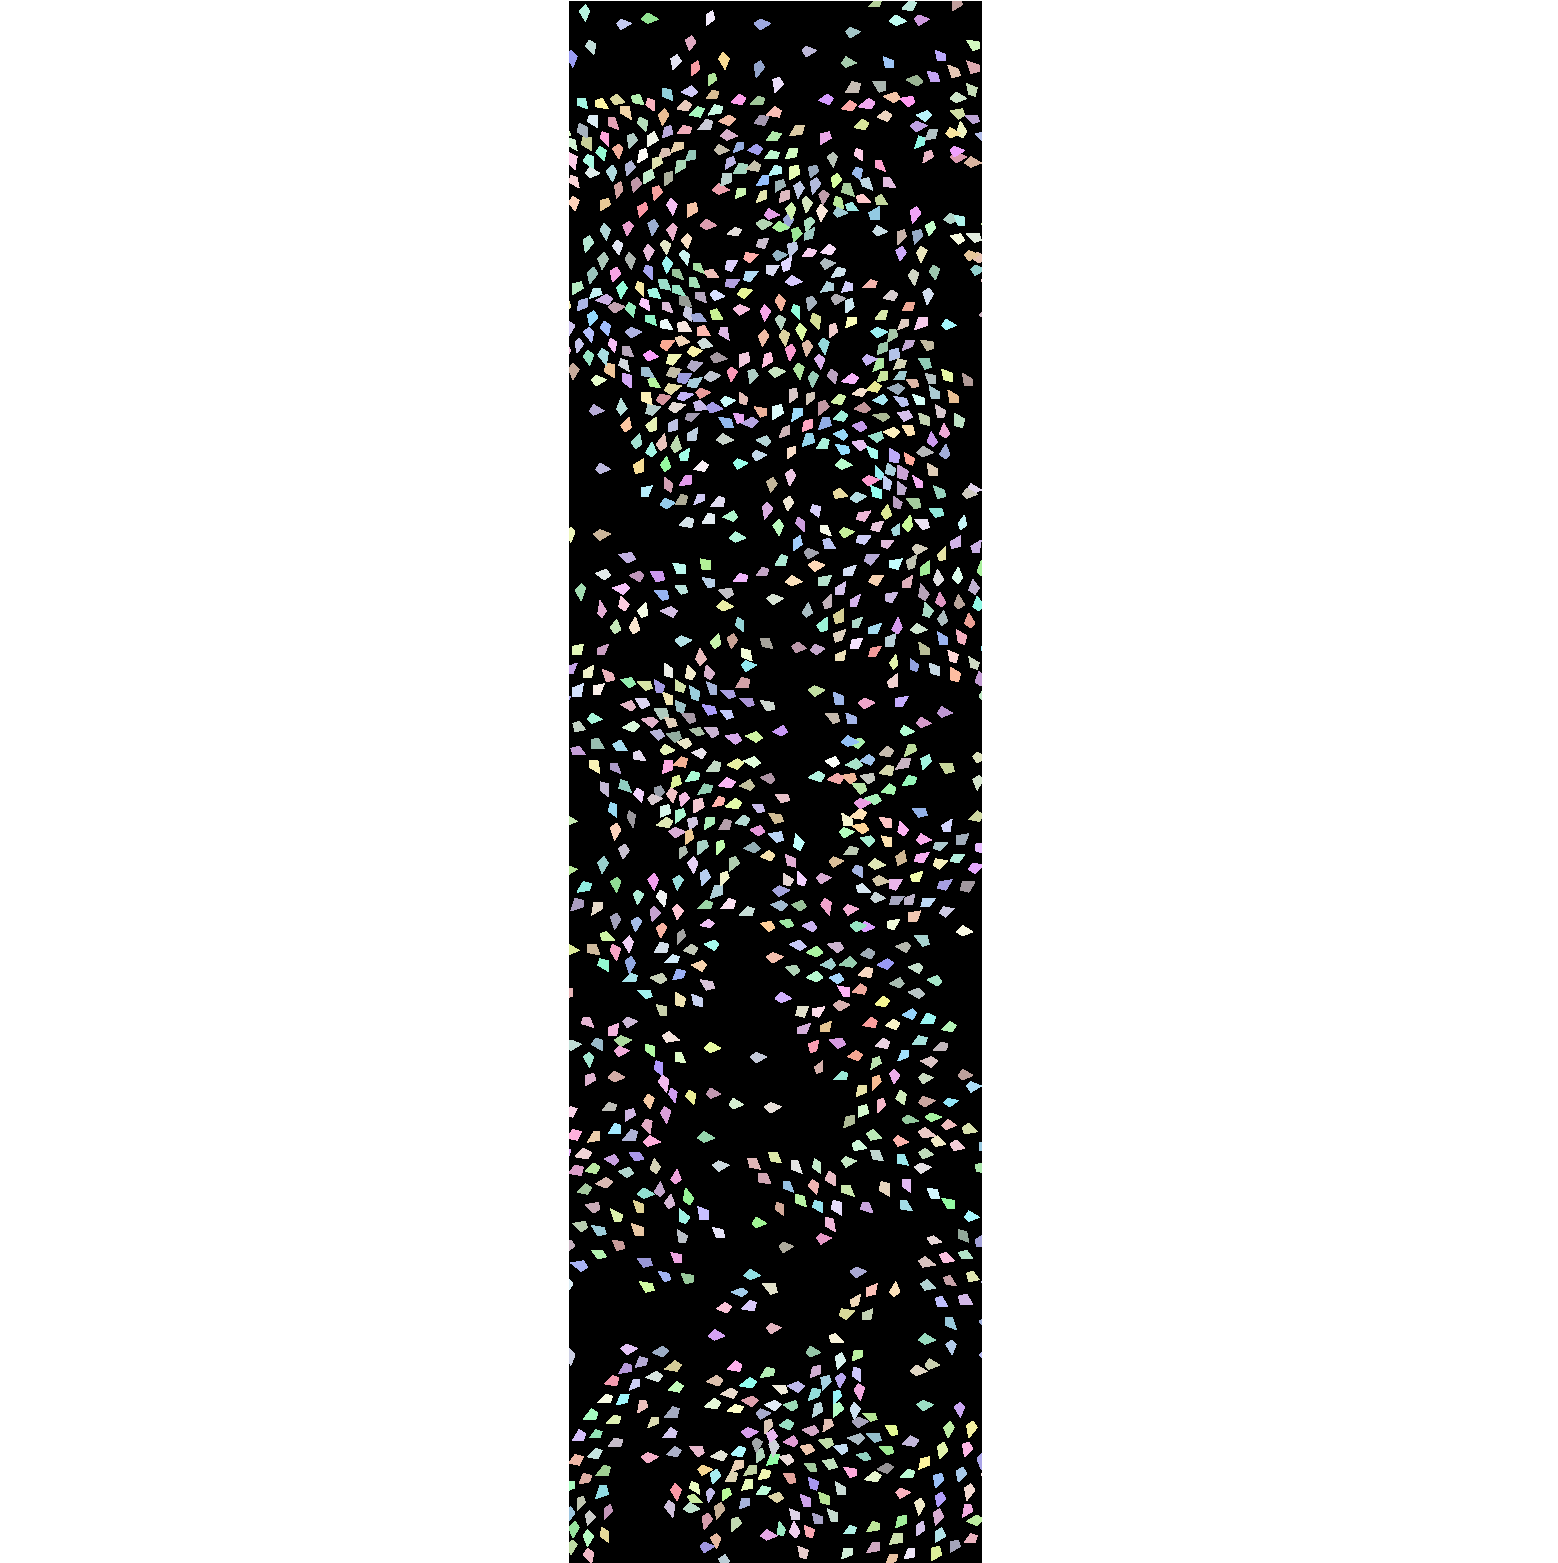
\includegraphics[height=11in]{Flockers.pdf}\end{wrapfigure}

\noindent\huge\bf \booktitle\\
\\
%{\large\rm A User Manual for the MASON Multiagent Simulation Toolkit}\\
\\
\Large\bf Sean Luke\\
{\large\rm 
Department of Computer Science\\
George Mason University}
\\
\\
\\
\large\rm {\bf Manual Version 19}\\
\large\rm June, 2015\\

\vspace{5in}
\noindent\Large\bf Where to Obtain MASON\\
\large\rm http:/\!/cs.gmu.edu/\!\(\sim\)eclab/projects/mason/

\clearpage

\small 
\noindent {\Large\bf Copyright }  2010--2015 by Sean Luke.

\vspace{0.25in}
\noindent {\Large\bf Thanks to } Claudio Cioffi Revilla and Carlotta Domeniconi.

\vspace{0.25in}

\noindent {\Large\bf Get the latest version of this document or suggest improvements here:}

\reference{http:/\!/cs.gmu.edu/\!\(\sim\)eclab/projects/mason/}

\vspace{0.15in}

\vspace{0.15in}
	\noindent {\Large\bf This document is licensed} under the {\bf Creative Commons Attribution-No Derivative Works 3.0 United States License,} except for those portions of the work licensed differently as described in the next section. To view a copy of this license, visit http:/\!/creativecommons.org/licenses/by-nd/3.0/us/ or send a letter to Creative Commons, 171 Second Street, Suite 300, San Francisco, California, 94105, USA.  A quick license summary:
	\begin{itemize}
	\item You are free to redistribute this document.
	\vspace{-0.5em}\item {\bf You may not} modify, transform, translate, or build upon the document except for personal use.   
	\vspace{-0.5em}\item You must maintain the author's attribution with the document at all times.
	\vspace{-0.5em}\item You may not use the attribution to imply that the author endorses you or your document use.  
	\end{itemize}
	This summary is just informational: if there is any conflict in interpretation between the summary and the actual license, the actual license always takes precedence.

\vspace{0.15in}

\noindent {\Large\bf This document is was produced} in part through funding from grants 0916870, 1205626, and 1317813 from the National Science Foundation.



\normalsize
\cleardoublepage

\tableofcontents
\clearpage


\chapter{Introduction}

\begin{figure}[h]\vspace{-33em}\hspace{30em}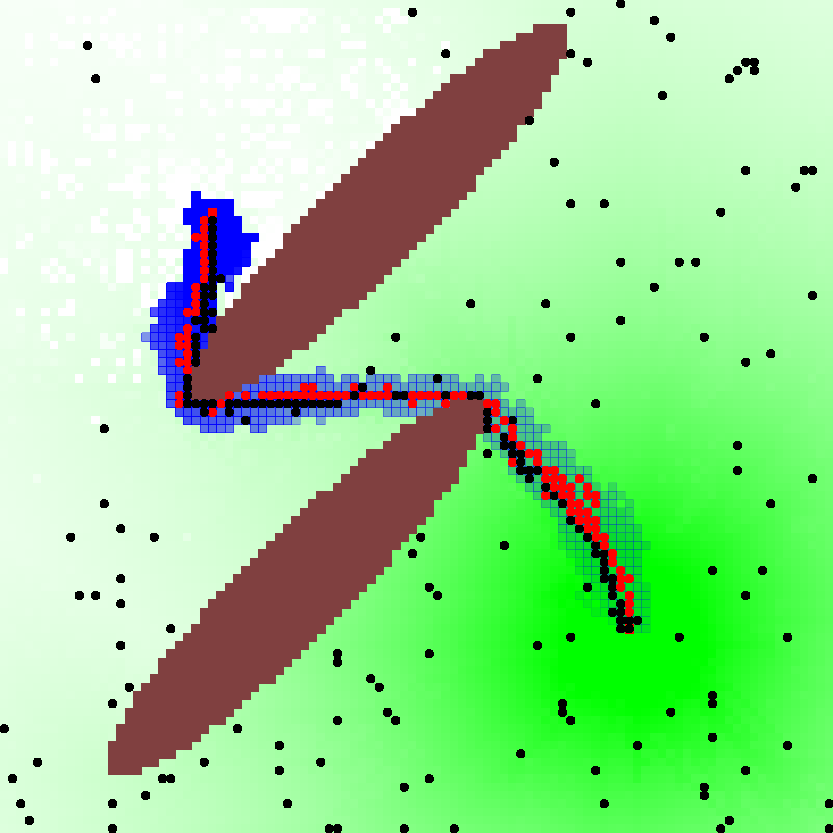
\includegraphics[width=4in]{ants.pdf}\vspace{2em}\end{figure}

MASON is a multiagent simulation toolkit designed to support large numbers of agents relatively efficiently on a single machine.  MASON has no domain-specific features: it is not a robotics simulator like TeamBots or Player/Stage, nor is it a game library.  Instead it belongs in the class of domain-independent simulators which might be unfairly described as ``dots on a screen'' simulators, such as Repast, Ascape, StarLogo, NetLogo, and of course, the venerable SWARM.

I call these simulators ``ultra-lightweight'' multiagent simulation toolkits.  They're popular for problems which involve many relatively simple agents and arbitrary problems, and are common in areas like artificial life, population biology, computational social sciences, complexity science, artificial intelligence, and (in my case) swarm robotics and mulitrobotics.

I use ultra-lightweight multiagent simulation toolkits because of previous experience in domain-specific ones.  Among other things, I do research in swarm robotics and multirobotics, but often apply it to other scenarios (vehicular traffic, crowds of people, etc.), and have found that it's easier and {\it much less buggy} to add domain features to a general toolkit than it is to strip out features from a domain-specific one.  The process of stripping out features, or working around them, leads to all sorts of dangling stuff which bites you in the end.  I'm sure this isn't an uncommon experience among simulation writers.

Most of these toolkits were developed for small jobs.  MASON is distinguished among these simulators because it is meant for big tasks involving a large number of simulation runs, likely on back-end server machines such as a supercomputer.  As such it has quite a number of features to help in this scenario.

\begin{itemize}
\item MASON models are fully separated from visualization. You can easily run a model without visualization or with various different kinds of visualization, and switch among them.
\item MASON models are entirely serializable to disk.  This means that you can checkpoint files in case your back-end server goes down, and restart form your latest checkpoint.  It also means you can run a MASON model on a back-end Linux machine, pause and serialize it to disk, move it to your Mac, unpause it under visualization, modify it, pause it again, move it to a PC, unpause it under a {\it different} visualization, pause it again, then put it back out on a back-end Sun server, and it'll continue to run happily as if nothing had happened.  
\item MASON models are entirely encapsulated.  This means you can run multiple MASON models in parallel in the same process, interleaved in a big for-loop, or in separate threads, and they'll not touch each other.
\item MASON is written in Java in order to make it easy to run in heterogeneous computer environments.  But it also is written in very carefully written Java, with an eye firmly fixed towards efficiency.  Notably, a number of poorly-written standard Sun classes are replaced with properly written MASON equivalents.  Java has a reputation for being slow, but this is largely due to Sun's bad libraries and design decisions (generics and boxing, iterators, etc.).  MASON eschews these internally.
\item MASON has a high-quality random number generator (Mersenne Twister) and uses the fastest known implementation of it.
\item MASON models are largely {\it duplicable},\footnote{Not to be confused with {\it replicable}: where the model can be built again in (say) NetLogo and it'll more or less run the same.  That's also true for MASON, but it's in some sense a lower standard.} meaning that if you run the simulation with exactly the same parameters (including random number seed) it'll run exactly the same way, even on different machines.\footnote{Well, that's not quite true.  MASON doesn't use the \variable{strictfp} keyword or the \class{java.lang.StrictMath} class, so if you move to a different CPU you may get slightly different floating point results.  However if you want to guarantee full duplicability, you can add the \variable{strictfp} keyword and replace \class{java.lang.Math} references with \class{java.lang.StrictMath} and everything should be perfectly duplicable, albeit slower.}
\item MASON dovetails nicely with ECJ\footnote{http:/\!/cs.gmu.edu/\(\sim\)eclab/projects/ecj/}, a very popular evolutionary computation (genetic algorithms, etc.) toolkit I wrote, which is designed (not surprisingly) for everything from single laptops to  large jobs involving thousands of machines.
\item MASON is modular and consistent.  There is a high degree of separation and independence among elements of the system.  This allows you to use, and recombine, different parts of the system in unexpected ways.  MASON is very highly hackable.  Indeed, a number of MASON's classes are used, with our blessing, in MASON's competition.\footnote{Well, not really competition: we're all friends here.}
\end{itemize}

Many of these features are quite common among good simulation libraries.  But not among those in the ``ultra-light'' multiagent simulation category.  In this area, MASON was {\it completely unique} when it was developed.  Since then, MASON's features have influenced the restructuring of other toolkits to include some of the above, but I believe that MASON still remains very much the high-performance, high-hackability leader among systems in this area.

\paragraph{What MASON is Not}
MASON is {\it not} a distributed toolkit.  Yet.  MASON was designed to be efficient when running in a single process, albeit with multiple threads.  It requires a single unified memory space, and has no facilities for distributing models over multiple processes or multiple computers.  However, there are several projects underway towards developing distributed versions of MASON.

MASON is {\it not} an easy toolkit for Java beginners.  MASON expects significant Java knowledge out of its users.  If you are a rank beginner, allow me to recommend NetLogo,\footnote{http:/\!/ccl.northwestern.edu/netlogo/} a good toolkit with an easy-to-learn language.

Finally MASON does {\it not} have plug-in facilities for Eclipse or NetBeans, though it can be used quite comfortably with them.  If you're looking for a richer set of development tools, you might look into Repast.\footnote{http:/\!/repast.sourceforge.net/}

\paragraph{MASON History}  In 1998, after using a variety of genetic programming and evolutionary computation toolkits for my thesis work, I decided to develop ECJ, a big evolutionary computation toolkit which was meant to support my own research for the next ten years or so.  ECJ turned out pretty well: it's used very widely in the evolutionary computation field and can run on a lot of machines in parallel.  ECJ was written in Java.

One common task (for me anyway) for evolutionary computation is the optimization of agent behaviors in large multiagent simulations.  ECJ can distribute many such simulations in parallel across simultaneous machines.  But the number of simulations that must be run (often around 100,000) makes it fairly important to run them very efficiently.  For this reason I and my students cooked up a plan to develop a multiagent simulation toolkit which could be used for various purposes, but which was fast and had a small and clean model, and so could easily be tied to ECJ to optimize, for example, swarm robotics behaviors.  Because ECJ was in Java, we expected our toolkit would be in Java as well.

As we got started, I spoke with Claudio Cioffi-Revilla, who was also interested in developing a toolkit for the computational social sciences.  Whereas our needs tended to be more continuous movement in 2D and 3D, many of his needs involved gridworlds and social networks.  Claudio suggested we take apart Repast and examine it.  We did, but ultimately followed my instinct to reinvent the wheel, and started work on MASON.  Ultimately the computer science department (myself and my students) and the Center for Social Complexity (Claudio and his students and faculty) teamed up to develop and fund MASON.  When MASON debuted at the Agent 2003 conference, it had model separation and encapsulation, duplicability, checkpointing, and 3D graphics, all of which is pass\'e in simulators, but was new to the ultralight simulation field.

Since then MASON has developed considerably.  It now has much more visualization, charting, selection, an improved Schedule, movable and selectable objects, etc. Claudio's influence has also been significant: MASON has extensive gridworld facilities, an external social networks package, and an external GIS facility.

I think MASON has done pretty well: it's fast and clean and has a small, modular, and orthogonal model.  It's had a strong influence (I think) on other toolkit development in the field, particularly Repast.  And MASON has been used for everything from small gridworld simulations to learning from demonstration on real robots to game development to large (up to millions of agents) simulations of fish, economic agents, swarm robots, and unmanned aerial vehicles.

\paragraph{What MASON Stands For} It's a backronym, for which the blame may be placed squarely on the shoulders of John Grefenstette.  Notionally it stands for Multi-Agent Simulation Of ... (we can't figure out a good ``N'').  Claudio likes to add ``Neighborhoods and Networks'', but that'd be NaN!

\section{Architectural Layout}

\begin{wrapfigure}{r}[0in]{3.7in}
\vspace{-4em}\hfill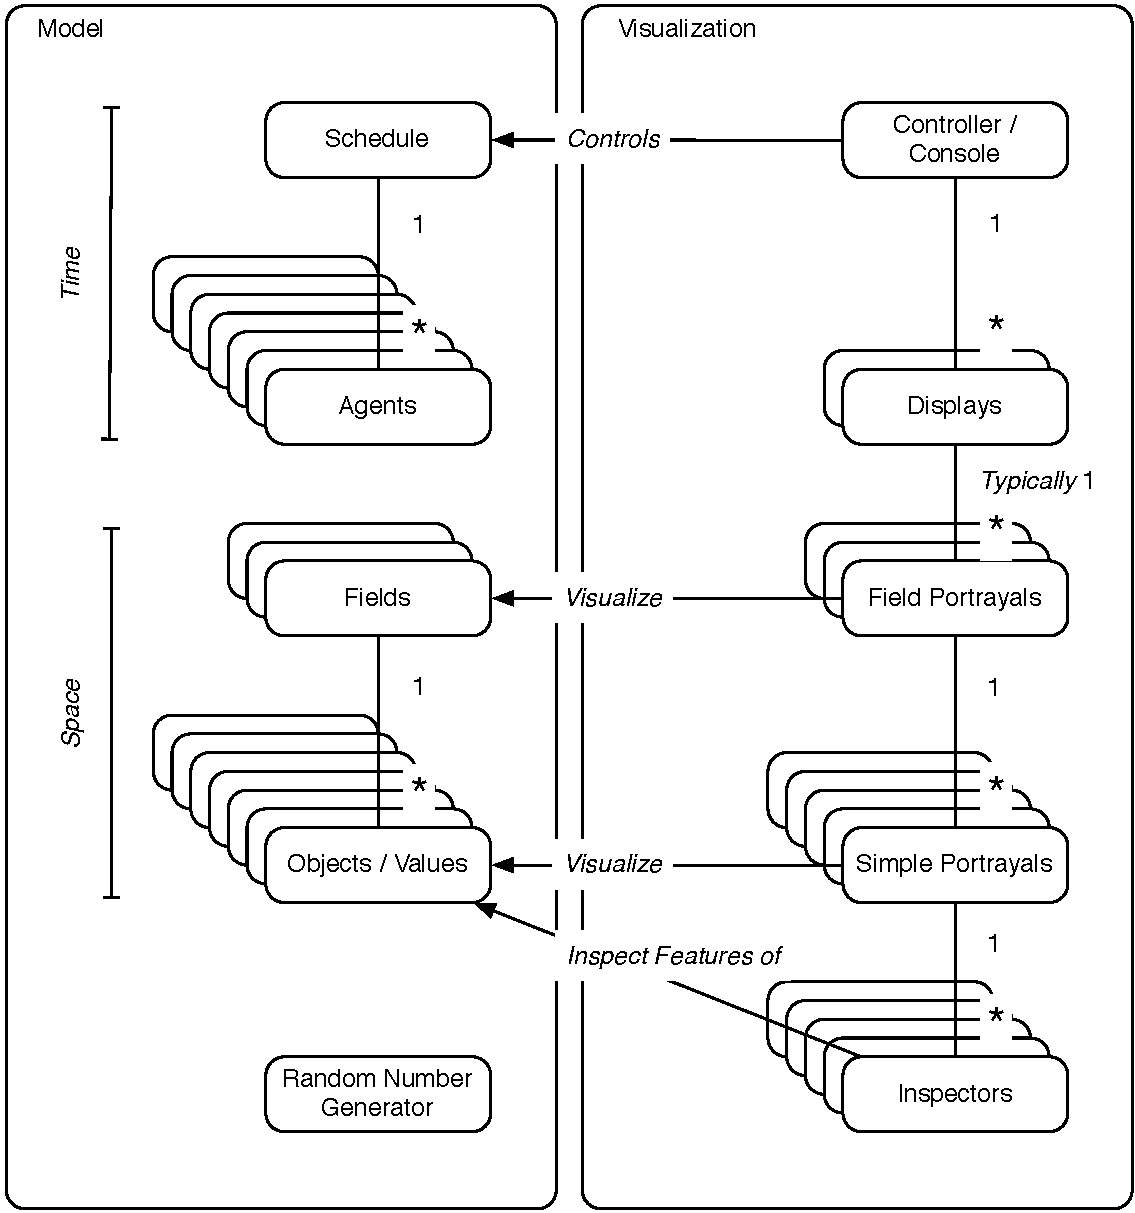
\includegraphics[width=3.7in]{MASONLayout.pdf}\vspace{-3em}\end{wrapfigure}

MASON is broken into two pieces.  The first part is the {\bf model} (the simulation proper) and the second part is the {\bf visualization}, presently either in 2D or in 3D.  Except when you choose to have model objects display themselves, the model and visualization are entirely separated.  This means that the model can be run without visualization; run with visualization of different sorts; and have its visualization changed, added, or removed at any time.  The model can also be {\bf checkpointed}, meaning it can be frozen and written out to disk, to be thawed out and continued even on another kind of computer.

At right is a general overview of the MASON architecture.

\paragraph{Model}  MASON's model is entirely encapsulated in a special object called \class{sim.engine.SimState}.  It contains a discrete event {\bf schedule} on which you can schedule various {\bf agents} to be called at some time in the future.  This facility is a MASON model's representation of {\bf time}. Additionally, the model contains one or more {\bf fields} to represent {\bf space}.  A field is nothing more than an arbitrary data structure relating various {\bf objects} or {\bf values} together.  MASON provides a number of built-in fields, such as networks, continuous space, and grids.  Last but not least, MASON's model contains a high-quality {\bf random number generator}.

\paragraph{Visualization} MASON provides both 2D and 3D visualization tools for models: and various plug-in facilities provide additional visualization (such as for GIS).  A visualization is encapsulated in an object called a\class{sim.display.GUIState}.  This contains an object called a {\bf controller} whose job is to start, stop, and otherwise manipulate the schedule.  The most common controller is a window called a {\bf console}.  The controller or console also manages some number of windows called {\bf displays}, which handle 2D or 3D visualization.  Displays visualize fields using one or more {\bf field portrayals}.  A field portrayal often (but not always) visualizes individual objects or values in fields by calling forth a {\bf simple portrayal} designed to visualize that particular object or value. Finally, after selecting objects with the mouse, simple portrayals often create {\bf inspectors} which provide further inspection of model details.

\paragraph{Utilities} MASON has a large set of utilities to support model design.  These include random number distributions, various collections objects, objects for inspecting Java Bean Properties, points in space, a host of GUI widgets, movie and picture generation, and chart generation.  Many of MASON's utility objects have since found their way into other agent-based simulation toolkits.

\paragraph{Demo Applications} MASON comes with many demos and tutorials, all of which are stored in the same directory, \file{app}. 

\section{Unpacking MASON}  When you download and unzip MASON, you'll get a directory consisting of the following things:

\begin{itemize}
\item A \file{CHANGES} file detailing all changes made to MASON since its inception.
\item A \file{LICENSE} file describing MASON's open-souce license.  Most of MASON uses the Academic Free License (AFL) 3.0.  This is a BSD-style license.  Those few classes which are not distributed as AFL fall under other BSD-style licenses.  AFL is very liberal, but if for some reason you have difficulty with this license, contact me and we can discuss other options.
\item A top-level \file{README} file describing how to start up MASON and where to go.
\item A \file{Makefile}.  MASON does not use Ant: I'm an old Unix hacker.  The Makefile can be used to build the 2D MASON facilities, to build the 3D facilities, to clean it, to indent all the code using Emacs, or to build a jar file.
\item A \file{docs} directory, containing all documentation on the system.
\item A \file{start} directory, containing double-click-on-me scripts for firing up MASON easily on various operating systems.
\item A \file{sim} directory.  This is the top-level package for MASON class files.
\item An \file{ec} directory.  This is the top-level package for the Mersenne Twister random number generator (shared with ECJ, hence the ``ec'').
\end{itemize}

\paragraph{Installing Libraries}
You'll need to install some libraries to make full use of MASON, and they're required if you're going to compile anything (and you're almost certainly going to want to do that!)  The libraries may be found on the MASON web page\footnote{http:/\!/cs.gmu.edu\(\sim\)eclab/projects/mason/}, and consist of the following:

\begin{itemize}
\item The JFreeChart charting library.
\item The iText PDF generation library.
\item (For OS X users only, optional) The Quaqua graphical interface extensions.
\item The Java Media Framework toolkit for building movies
\end{itemize}

Additionally you'll want to install the Java3D toolkit if you're doing 3D.  On OS X Java3D is already installed.  On Windows or Linux you'll have to download and install it.  See the MASON web page for instructions.

\section{Running MASON}

MASON is run in two ways: either by running an application directly, or by firing up MASON's console.  If you build MASON's jar file, you can double-click on it or otherwise run it, and the console will pop up.  Alternatively you can run the console by first adding the \file{mason} directory to your CLASSPATH, then running:

\script{\textit{java sim.display.Console}}

\indent You can run individual demo applications too (they're all in the \file{sim/app} directory), for example:

\script{\textit{java sim.app.heatbugs.HeatBugsWithUI}}

\indent Various scripts in the \file{start} directory can do all this for you automatically, depending on your OS.  Note that certain Java3D applications suck up a lot of memory and will require more RAM.  You can add more memory when running java like this:

\script{\textit{java -Xmx500M -Xms500M sim.display.Console}}

\indent This example causes MASON to be run with 500 megabytes of available virtual memory.

More information on Running MASON can be found in the \file{README} file and also in the \file{docs/index.html} file.  On the website you can also find a tutorials for running an (earlier version of) MASON on NetBeans and Eclipse.

\section{Additional MASON Modules}

MASON has a variety of add-on modules which extend MASON in various ways.  They don't come with the main package but you can easily download them from the website.  Some public extensions include:

\begin{itemize}
\item GeoMason: GIS extensions to MASON, developed by Marc Colletti and Keith Sullivan.
\item Rigid-body 2D Physics, developed by Christian Thompson.
\item Social Networks.  A package developed by Liviu Panait and Gabriel Balan.
\item Examples for how to use JUNG (a social networks package) and MASON.  By Maciej Latek.
\end{itemize}

Some of these packages may be found in the ``contrib'' directory of MASON's SVN repository on Google Code.  Various groups have also added stuff to this directory.


\chapter{Tutorial: Student Schoolyard Cliques}

\begin{figure}[h]\vspace{-39em}\hspace{-5em}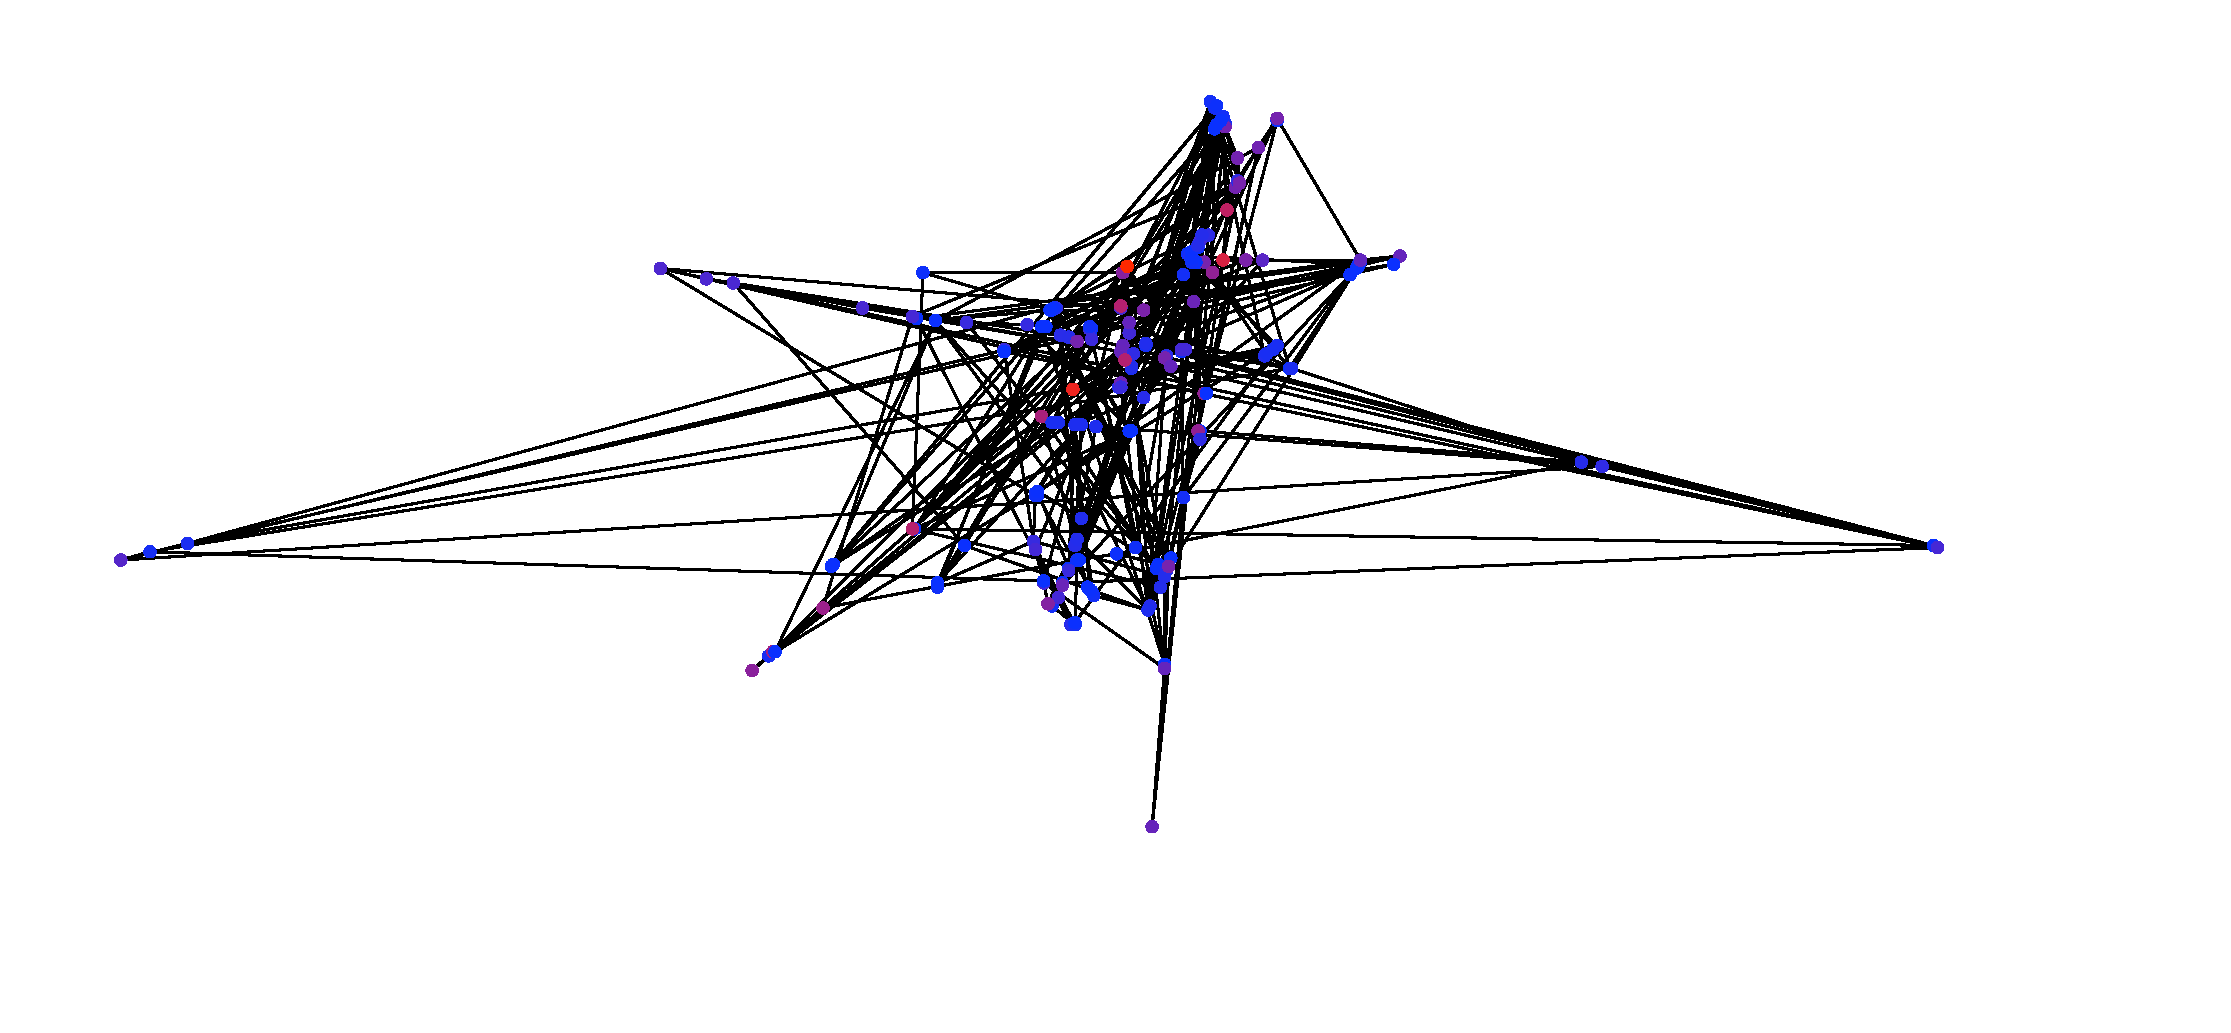
\includegraphics[width=12in]{Cliques.pdf}\end{figure}

\noindent In this tutorial sequence we will build a simple social network spread throughout the 2-dimensional continuous space of a schoolyard with a school (and notional teacher) at the center.\footnote{This tutorial sequence was originally developed for the World Congress on Social Simulation in 2008.}  

\section{Create an Empty Simulation}Let's begin simply, with a MASON application that does absolutely nothing.
\label{CreateAnEmptySimulation}

\paragraph{Create the file Students.java} Place in it the text:

{\footnotesize \begin{alltt}
import sim.engine.*;

public class Students extends SimState
    \{
    public Students(long seed)
        \{
        super(seed);
        \}

    public static void main(String[] args)
        \{
        doLoop(Students.class, args);
        System.exit(0);
        \}    
    \}
\end{alltt}
}

Wow, it doesn't get a whole lot simpler (and more useless) than that.

When you create a MASON application, you define the simulation model as a subclass of \Class{sim.engine.SimState}.  MASON will create a single instance of this subclass and maintain it as the global state of your entire simulation.  SimState contains two important items:

\begin{itemize}
\item A {\bf random number generator}, specifically an instance of the class \class{ec.util.MersenneTwisterFast}.  This generator is far better than \Class{java.util.Random}. It is also not synchronized, which means that if you access it from multiple threads, you'll need to remember to acquire a lock on it first.  We'll get to that later.  Anyway, if you're serious about simulation, you should {\bf never use \Class{java.util.Random} nor \method{java.lang.Math.random()}.}  They're surprisingly poor quality.\footnote{\Class{java.util.Random} is highly non-random, and will ruin your experiments.  And \method{Math.random()} just uses \Class{java.util.Random}. Don't use them.  For a fun example of just how bad \Class{java.util.Random} is, check out ``Sun Redefines Randomness'': http:/\!/alife.co.uk/nonrandom/}

The random number generator is seeded with a random number {\bf seed}, a long integer passed into the SimState's constructor as shown in the code above.  Note that MersenneTwisterFast only uses the first 32 bits of this seed.

\item A {\bf discrete event schedule}, an instance of the class \Class{sim.engine.Schedule} (or a subclass).  You will schedule {\bf agents} onto this schedule to be {\bf stepped}: woken up at various times in the simulation to do their thing.  The Schedule is your simulation's representation of time.
\end{itemize}

\sidebar{Why call \code{System.exit(0)}?  Why not just exit normally?}{Because if you forgot to terminate any threads created while running a MASON simulation, and forgot to declare all of your threads to be {\it daemon threads}, then after \code{main(...)} exits, those threads will continue to run and your simulation will not quit.  Calling \code{System.exit(0)} ensures that uncooperative threads will be killed.}

When you compile and run this MASON application, the \method{doLoop(...)} method is called, passing in the simulation class and the command-line arguments, and then the application terminates with a \method{System.exit(0)}.  The \method{doLoop(...)} performs an elaborate simulation loop with a lot of built-in gizmos, but the basic concept is actually a very simple top-level loop:

\begin{enumerate}
\item Create an instance of your SimState subclass, initializing its random number generator with a seed of some sort (perhaps the current time).
\item Call \method{start()} on the instance allow you to initialize your simulation model.  (We didn't implement this method because we have nothing to initialize yet).
\item Repeatedly call \method{step(SimState state)} on the instance's discrete-event schedule, pulsing it and causing agents stored in the schedule to be stepped.
\item When the schedule is entirely empty of agents (which for us is immediately\,---\,we scheduled none), or after some \(N\) calls to \method{step(...)} have been made on the schedule, call \method{finish()} on the instance to let it clean up.  This method is rarely used.
\end{enumerate}

As mentioned before, the \method{doLoop(...)} method has lots of gizmos, but in fact, we could have written a simple version of \method{main(...)} like this:

{\footnotesize \begin{alltt}
    public static void main(String[] args)
        \{
        SimState state = new Students(System.currentTimeMillis());
        state.start();
        do
            if (!state.schedule.step(state)) break;
        while(state.schedule.getSteps() < 5000);
        state.finish();
        System.exit(0);
        \}
\end{alltt}
}

All \method{doLoop(...)} does for us is provide a number of useful ways of controlling MASON from the command line.  We can create checkpoints (freeze simulations in time and save them to disk), start up from a previous checkpoint, run for a certain number of steps; until a certain point in ``simulation time'', run multiple jobs in sequence, etc.

\paragraph{Compile and Run} 
Let's compile and run this sucker.  Presuming MASON has been added to your CLASSPATH...

{\footnotesize \begin{alltt}
\textit{javac Students.java
java Students}

MASON Version 15.  For further options, try adding ' -help' at end.
Job: 0 Seed: 1293295240209
Starting Students
Exhausted
\end{alltt}}

\sidebar{How do I run this on Eclipse or Netbeans?}{Stay Tuned... }

MASON starts by printing its version, then the job number and the random number seed for the job.  It then states it's starting Students, and finally states that it quit because the schedule was {\bf exhausted}, that is, it had no more agents to step.

\section{Add Some Students}

We next create a schoolyard and add some students to it.  The students won't do anything yet\,----\,they're not really agents until we add them to the schedule.  We'll just put them in random locations.  Here's the changes we make to \file{Students.java}:

{\footnotesize \begin{alltt}
{\color{gray}import sim.engine.*;}
import sim.util.*;
import sim.field.continuous.*;

{\color{gray}public class Students extends SimState
    \{}
    public Continuous2D yard = new Continuous2D(1.0,100,100);
    public int numStudents = 50;

    {\color{gray}public Students(long seed)
        \{
        super(seed);
        \}}

    public void start()
        \{
        super.start();
        
        // clear the yard
        yard.clear();
        
        // clear the buddies
        buddies.clear();
        
        // add some students to the yard
        for(int i = 0; i < numStudents; i++)
            \{
            Student student = new Student();
            yard.setObjectLocation(student, 
                new Double2D(yard.getWidth() * 0.5 + random.nextDouble() - 0.5,
                    yard.getHeight() * 0.5 + random.nextDouble() - 0.5));
            \}
        \}
        
     {\color{gray}public static void main(String[] args)
        \{
        doLoop(Students.class, args);
        System.exit(0);
        \}
    \}}
\end{alltt}}

First notice that we have added two variables to the \class{Students} class: the yard where the students exist, and the number of students.  The yard will be one of our {\bf representations of space} (we'll add the network in a moment).  In MASON parlance, representations of space, which are typically displayed in the GUI, are called {\bf fields}.  A field is a generic term: you can make your own data structure if you like.  But MASON provides a number of built-in fields for your convenience, and this is one of them: the class \Class{sim.field.continuous.Continuous2D}.

The Continuous2D class defines a 2-dimensional environment of real-valued (continuous) space.  The space may be bounded, toroidal, or infinite (unbounded): here we're going to assume it's unbounded, though we'll specify some bounds for drawing purposes later.  Our bounds are 100 by 100.  Furthermore, the Continuous2D discretizes its space into an underlying grid to make neighborhood lookups easier: we don't use that feature so we just use 1.0 as our discretization (it doesn't make any difference).

We have also added a \method{start()} method.  Recall that this method is called before the schedule is stepped in order to allow the simulation to set itself up.  The first thing we do in this method is call \code{super.start()}, which is very important.

We then use this method to set up the yard: we clear it of objects (the students), and then we add 50 students to the yard at random locations.

\sidebar{Why use Double2D?  Why not use Point2D.Double?}{Because Point2D.Double is {\it mutable}, meaning that its X and Y values can be changed once set.  As a result, Point2D.Double is not safe as a key in a hash table.  And Continuous2D uses hash tables to store its objects.

You'll see Double2D and its friends (Int2D, Double3D, and Int3D) a lot.  They're very simple classes which store {\it immutable} pairs or triples of doubles or ints.  Once you set the values, you cannot change them\,---\,you'll need to make a new object\,---\,and this makes them safe for use in classes relying on hash tables.

You can easily convert between these classes and similar Java classes, such as Point or Point2D.Double.}

A Continuous2D can hold objects of any kind and associates each one of them with a 2-dimensional point in space, specified by a \Class{sim.util.Double2D} object.  Notice that we produce the X and Y values of the Double2D by choosing two small random double values from [-0.5...0.5), and adding them to the dead center of the yard.   But the yard is 100x100!   This places all the students in the range X=[49.5...50.5) and Y=[49.5...50.5), all clustered right around the center.  This is, we presume the location of the schoolhouse where the students have just gotten out of class.

Now we need to define what a Student is.  We'll start with nothing:

\paragraph{Create the file Student.java} Place in it the text:

{\footnotesize \begin{alltt}
public class Student
    \{
    \} 
\end{alltt}}


\paragraph{Compile and Run}  We compile and run similar to before, and get basically the same thing (since our Students aren't {\it doing} anything yet).

{\footnotesize \begin{alltt}
\textit{javac Students.java Student.java
java Students}

MASON Version 15.  For further options, try adding ' -help' at end.
Job: 0 Seed: 1293298122803
Starting Students
Exhausted
\end{alltt}}

Note that the seed has changed.  It's based on the current wall clock time.  If you'd like to fix the seed to a specific value (say, 4), you can do this (triggering a feature in \method{doLoop(...)}):

{\footnotesize \begin{alltt}
\textit{java Students -seed 4}

MASON Version 15.  For further options, try adding ' -help' at end.
Job: 0 Seed: 4
Starting Students
Exhausted
\end{alltt}}

Very exciting.

\section{Make the Students Do Something}

We next will create two simple forces: a force which causes the students to wander randomly, and a force which draws them to the schoolteacher notionally at the school at the center of the yard.  We'll schedule the students on the schedule and have them wander about under the guidance of these forces.

We begin by modifying the \file{Students.java} file, adding two new variables for these forces, and also scheduling each student on the Schedule.

{\footnotesize \begin{alltt}
{\color{gray}import sim.engine.*;
import sim.util.*;
import sim.field.continuous.*;

public class Students extends SimState
    \{
    public Continuous2D yard = new Continuous2D(1.0,100,100);
    public int numStudents = 50;}
    double forceToSchoolMultiplier = 0.01;
    double randomMultiplier = 0.1;

    {\color{gray}public Students(long seed)
        \{
        super(seed);
        \}

    public void start()
        \{
        super.start();
        
        // clear the yard
        yard.clear();
        
        // clear the buddies
        buddies.clear();
        
        // add some students to the yard
        for(int i = 0; i < numStudents; i++)
            \{
            Student student = new Student();
            yard.setObjectLocation(student, 
                new Double2D(yard.getWidth() * 0.5 + random.nextDouble() - 0.5,
                    yard.getHeight() * 0.5 + random.nextDouble() - 0.5));}

            schedule.scheduleRepeating(student);
            {\color{gray}\}
        \}
        
    public static void main(String[] args)
        \{
        doLoop(Students.class, args);
        System.exit(0);
        \}
    \}}
\end{alltt}}

There are many methods for scheduling agents on the Schedule.  This is one of the simplest: it schedules an agent to be stepped\footnote{Or ``pulsed'', or ``called'', or ``made to receive an event'', or whatever you like to call it.  I say ``stepped''.}, every 1.0 units of time, starting 1.0 units from now.  The Schedule starts at time 0.0.  Since all the Students are being scheduled like this, each one of them will be stepped at timestep 1.0, then at 2.0, then at 3.0, and so on.  Since we have not specified a sorting priority among them, each timestep the Students will be stepped in random order with respect to one another.

Now say what these Students will do when stepped.  We define their \method{step(...)} methods:

{\footnotesize \begin{alltt}
import sim.engine.*;
import sim.field.continuous.*;
import sim.util.*;

{\color{gray}public class Student} implements Steppable
    {\color{gray}\{}
    public void step(SimState state)
        \{
        Students students = (Students) state;
        Continuous2D yard = students.yard;

        Double2D me = students.yard.getObjectLocation(this);

        MutableDouble2D sumForces = new MutableDouble2D();

        // add in a vector to the "teacher" -- the center of the yard, so we don't go too far away
        sumForces.addIn(new Double2D((yard.width * 0.5 - me.x) * students.forceToSchoolMultiplier, 
                (yard.height * 0.5 - me.y) * students.forceToSchoolMultiplier));
        
        // add a bit of randomness
        sumForces.addIn(new Double2D(students.randomMultiplier * (students.random.nextDouble() * 1.0 - 0.5), 
                students.randomMultiplier * (students.random.nextDouble() * 1.0 - 0.5)));

        sumForces.addIn(me);

        students.yard.setObjectLocation(this, new Double2D(sumForces));
        \}
    {\color{gray}\}} 
\end{alltt}}

The first thing to notice is that Student implements the \Class{sim.engine.Steppable} interface by implementing the method \method{step(...)}.  By being Steppable, the Student can be placed on the Schedule to have its \method{step(...)} method called at various times in the future.  This graduates the Student from being a mere object in the simulation to being something potentially approximating a real  {\bf agent}.

When a Student is stepped, it is passed the SimState.  The first thing we do is cast it into the Students class (which it is), then extract our yard (the Continuous2D).

The student needs to know where it's located in the yard.  We could have stored the X and Y coordinates in the Student itself (which would be a bit faster) but can always just query the yard itself, which is what we do with \method{getObjectLocation(...)}.

\sidebar{Seriously, why not use Point2D.Double here?}{Mostly for consistency with Double2D and for the purpose of demonstration in this tutorial, that's all.  Plus MutableDouble2D has many of the same methods as Double2D, plus various useful methods like \method{addIn}.  If you want to use Point2D.Double, go right ahead, it'll work fine here.}

Now we'd like to move the object with some artificial forces.  We start with a \Class{sim.util.MutableDouble2D}, which is just like a Double2D except that you can change its X and Y values after the fact.  MutableDouble2D also has various sometimes-helpful modification methods like \method{addIn}.  Of course, instead of \code{foo.addIn(new Double2D(4,3))} you could instead write \code{foo.x += 4; foo.y += 3;} and be done with it (and it'd be faster too).  But we're just demonstrating here!

So.... we add in a force towards the center of the yard which increases with distance to the yard; and also a small constant random force.  Finally we the force to our present location, then set our location to the sum.  Notice that the location must be a Double2D, not a MutableDouble2D (it must be immutable!).

\paragraph{Compile and Run}  Here we go...

{\footnotesize \begin{alltt}
\textit{javac Students.java Student.java
java Students}

MASON Version 15.  For further options, try adding ' -help' at end.
Job: 0 Seed: 1293316557082
Starting Students
Steps: 50000 Time: 49999 Rate: 37,593.98496
Steps: 100000 Time: 99999 Rate: 54,704.59519
Steps: 150000 Time: 149999 Rate: 53,821.31324
Steps: 200000 Time: 199999 Rate: 54,824.5614
Steps: 250000 Time: 249999 Rate: 55,187.63797
Steps: 300000 Time: 299999 Rate: 54,585.15284
{\it ...etc...}
\end{alltt}}

Finally something new!  Since the Students are scheduled on the Schedule, they're stepped every timestep.  Every so often (roughly every second) the current step is printed out, plus the step rate.   the Students never vacate the Schedule (they're scheduled ``repeating''), this will go on forever.  We could instead run for a limited time like this:

{\footnotesize \begin{alltt}
\textit{java Students -time 200000}

MASON Version 15.  For further options, try adding ' -help' at end.
Job: 0 Seed: 1293318062046
Starting Students
Steps: 50000 Time: 49999 Rate: 37,821.4826
Steps: 100000 Time: 99999 Rate: 56,561.08597
Steps: 150000 Time: 149999 Rate: 58,004.64037
Steps: 200000 Time: 199999 Rate: 57,405.28129
Quit
\end{alltt}}

\sidebar{What's the difference between the Schedule's ``time'' and``steps''?}{You can schedule agents to be stepped at any real-valued {\it time}.  Each iteration (or {\it step}) of the Schedule, it looks for the timestamp of the earliest scheduled Steppable, advances the clock to that time, then extracts all the Steppables scheduled at that time and processes them. It so happens here that agents are all scheduled for timestamps of integers, so the time equals the steps more or less.  But that's not necessarily the case: we could have agents scheduled for every 3.923 units of time, say.}

This tells us that MASON ran until the specified time, then exited even though there were Steppable agents still scheduled on the Schedule (note the ``Quit'' as opposed to ``Exhausted'').

So far we're doing everything on the command line.  Time to...

\section{Add a GUI Control}

Note that so far everything we've done has been on the command line.  Let's move toward a graphical interface by first introducing a {\bf console} which allows us to start, stop, pause, step, and restart the simulation (among other things).

\paragraph{Create the file StudentsWithUI.java} Place in it the text:

{\footnotesize \begin{alltt}
import sim.engine.*;
import sim.display.*;

public class StudentsWithUI extends GUIState
    \{
    public static void main(String[] args)
        \{
        StudentsWithUI vid = new StudentsWithUI();
        Console c = new Console(vid);
        c.setVisible(true);
        \}

    public StudentsWithUI() \{ super(new Students(System.currentTimeMillis())); \}
    public StudentsWithUI(SimState state) \{ super(state); \}
    public static String getName() \{ return "Student Schoolyard Cliques"; \}
    \}
\end{alltt}}


MASON is somewhat unusual among multiagent simulation toolkits\footnote{But hardly unusual among big simulation toolkits in general in this respect.} in that it strictly distinguishes between an entirely self-contained and modular {\bf model}, and the {\bf visualization} or other {\bf controls}.  MASON thus largely adheres to the so-called ``MVC'' model (Model/View/Controller).  There's a bright line between the GUI and the model: indeed the model often has no knowledge of or reference to the GUI at all.  No GUI events are placed on the Schedule.

This has a number of advantages.  First and foremost, we can {\bf separate the model from the GUI} and run it on the command line (on a back-end supercomputer say), then occasionally save it, transfer it to a Windows box, and {\bf re-integrate it with a GUI} to visualize and modify the model.  Then save it and put it back out on the supercomputer to continue running. All of this can be done {\it in the middle of the simulation run}.  The model is none the wiser.

Second, we can attach {\bf different kinds of visualization} to the model at different times.  We could visualize portions of the model in 2D, then change the visualization to something in 3D, say.

\sidebar{Wait, what?  You can run two simulations in parallel?}{Sure, why not?  The models are  self-contained.  For example:

{\scriptsize \begin{alltt}
public static void main(String[] args)\\
\setlength\parindent{1.5em}\indent\{\\
\indent long time = System.currentTimeMillis();\\
{\indent}SimState state = new Students(time);\\
{\indent}SimState other = new Students(time + 212359234);\\
{\indent}state.start();\\
{\indent}other.start();\\
{\indent}while(true)\\
{\indent}{\indent} if (!state.schedule.step(state)\\
{\indent}{\indent}{\indent}\&\& !other.schedule.step(other)) break;\\
{\indent}state.finish();\\
{\indent}other.finish();\\
{\indent}System.exit(0);\\
{\indent}\}
\end{alltt}
}}

Third, because the model is self-contained, we can run multiple models at the same time, either interleaved in the same thread or on separate threads.  

Since MASON separates model and visualization, it has separate primary classes for each:

\begin{itemize}
\item The primary model class is a subclass of \Class{sim.engine.SimState}.
\item The class in charge of visualization is a subclass of \Class{sim.display.GUIState}.
\end{itemize}

In the code above we have created our GUIState subclass.  We named it 
\class{StudentsWithUI}.  In nearly all the MASON examples, when the SimState (model) is named {\bf \textit{Foo}}, then the GUIState is named {\bf \textit{Foo}WithUI}.  You hardly need to keep this tradition\,---\,feel free to name your UI class whatever you like\,---\,but if you want to be consistent, there you go.

The StudentsWithUI class usually has two constructors: a default (empty) constructor, and one which takes a SimState.  The default constructor simply creates an appropriate SimState, typically providing the current wall-clock time as the seed as shown, and passes it to the other constructor.

Subclasses of GUIState also provide a name for the simulation via the method \method{getName()}.  This name will appear in GUI controls to describe the simulation.

We also provide a new \method{main(...)} method.  Rather than create a simulation and run it, this method fires up the visualization (which handles creating the simulation on our behalf).  Here's what the GUIState's \method{main(...)} method must do:

\begin{itemize}
\item Create one of our GUIState subclasses.
\item Create a Console.  This is a GUI control which allows us to start/stop/pause/etc. the simulation.
\item Make the Console visible.
\end{itemize}

\noindent ...and that's just what our code does.

\begin{wrapfigure}{r}[0in]{3in}
\vspace{-6.5em}\hfill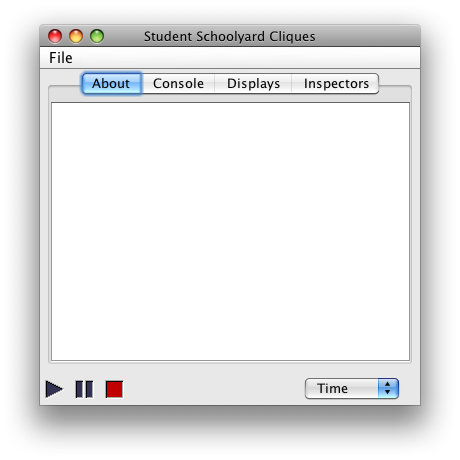
\includegraphics[width=2.8in]{Console.png}\vspace{-5em}\end{wrapfigure}

\paragraph{Compile and Run}  When we compile and run the code...

{\footnotesize \begin{alltt}
\textit{javac StudentsWithUI.java Students.java Student.java
java StudentsWithUI}
\end{alltt}}

\noindent ...we no longer get boring command-line results.  Instead, we get the window shown at right.  This is the {\bf Console}.  It's the command center for your simulation: it controls playing, pausing, and stopping the simulation; plus showing and hiding displays and inspector panels. You can save and load simulations to and from checkpoints and quit using the Console.

An introduction:

\begin{itemize}
\item[\raisebox{-0.25em}{
\includegraphics[scale=0.4]{PlayButton.png}}] The Play button.  Press this to start a simulation: the \method{start()} method is called on the SimState, followed by repeated calls to step the Schedule.
\item[\raisebox{-0.25em}{
\includegraphics[scale=0.4]{PauseButton.png}}] The Pause button.  Press this  to pause or unpause the simulation.  While paused, the Play Button changes to \raisebox{-0.25em}{
\includegraphics[scale=0.4]{StepButton.png}} the Step Button, which lets you step through the simulation.
\item[\raisebox{-0.25em}{
\includegraphics[scale=0.4]{StopButton.png}}] The Stop button.  Press this stop a running simulation: the \method{finish()} will be called on the SimState.
\item[\raisebox{-0.25em}{
\includegraphics[scale=0.4]{TimeButton.png}}] When a simulation is playing, either the current simulation time, steps, or rate is shown next to the Stop button.  This chooser lets you select which.
\item[\raisebox{-0.25em}{
\includegraphics[scale=0.4]{AboutButton.png}}] This tab displays descriptive simulation information of your choice as an HTML file (at present there isn't any, but wait).
\item[\raisebox{-0.25em}{
\includegraphics[scale=0.4]{ConsoleButton.png}}] This tab shows various widgets for manipulating the speed of the simulation, automatically pause or stop at a certain time, etc.
\item[\raisebox{-0.25em}{
\includegraphics[scale=0.4]{DisplaysButton.png}}] This tab shows the list of all visualization {\bf displays}.  At present we have none, but we will have one soon!
\item[\raisebox{-0.25em}{
\includegraphics[scale=0.4]{InspectorsButton.png}}] This tab shows the list of all current {\bf inspectors}\footnote{Some other multiagent simulation toolkits, following the Swarm tradition, use the term {\it probes}.  When building MASON I chose the term ``inspectors'', following the GUI tradition of NeXTSTEP and later OS X.} of objects in the simulation. At present we have none, we'll see them presently.
\item[\raisebox{-0.1em}{
\includegraphics[scale=0.4]{FileMenu.png}}] The {\bf Console Menu}, which allows to save and load simulations, choose new simulations, or quit.
\end{itemize}

\paragraph{Start the Simulation}  Press the Play Button and watch it go.  Not very interesting yet: because we don't yet have a {\bf visualization}.  That's next.

\section{Add Visualization}

Now we're getting somewhere!  The code below is more complex than we've seen so far, but it's not too bad.  We're going to add 2-dimensional visualization object called a \Class{sim.display.Display2D}.  This object is capable of displaying several fields at once, layered on top of one another.  We only have one field (the schoolyard, a Continuous2D).  Such an object, in MASON parlance, is called a {\bf display}.   Displays can sprout their own windows (\Class{javax.swing.JFrame}) to hold them, and we'll do that.

We will also attach to the Display2D a single {\bf field portrayal}.  This object is responsible for drawing and allowing inspection of a field (in our case, the schoolyard).  In our case, the field portrayal will be an instance of \Class{sim.portrayal.continuous.ContinuousPortrayal2D}.

The field portrayal will draw and inspect individual objects stored in the Continuous2D by calling forth one or more {\bf simple portrayals} registered with the field portrayal to draw those objects.  Our objects are students.  For our simple portrayal we'll choose a \Class{sim.portrayal.simple.OvalPortrayal2D}, which draws objects as gray circles (you can change the color).

First here's the code.  Afterwards we'll go through each of the new methods.  Notice the three new instance variables in our GUIState:

\begin{itemize}
\item The display.
\item The JFrame which holds the display.
\item The field portrayal responsible for portraying the yard. 
\end{itemize}

{\footnotesize \begin{alltt}
import sim.portrayal.continuous.*;
{\color{gray}import sim.engine.*;
import sim.display.*;}
import sim.portrayal.simple.*;
import javax.swing.*;
import java.awt.Color;

{\color{gray}public class StudentsWithUI extends GUIState
    \{}
    public Display2D display;
    public JFrame displayFrame;
    ContinuousPortrayal2D yardPortrayal = new ContinuousPortrayal2D();

    {\color{gray}public static void main(String[] args)
        \{
        StudentsWithUI vid = new StudentsWithUI();
        Console c = new Console(vid);
        c.setVisible(true);
        \}

    public StudentsWithUI() \{ super(new Students( System.currentTimeMillis())); \}
    public StudentsWithUI(SimState state) \{ super(state); \}
    public static String getName() \{ return "Student Schoolyard Cliques"; \}}
    
    public void start()
        \{
        super.start();
        setupPortrayals();
        \}

    public void load(SimState state)
        \{
        super.load(state);
        setupPortrayals();
        \}

    public void setupPortrayals()
        \{
        Students students = (Students) state;
        
        // tell the portrayals what to portray and how to portray them
        yardPortrayal.setField( students.yard );
        yardPortrayal.setPortrayalForAll(new OvalPortrayal2D());
        
        // reschedule the displayer
        display.reset();
        display.setBackdrop(Color.white);

        // redraw the display
        display.repaint();
        \}

    public void init(Controller c)
        \{
        super.init(c);
        display = new Display2D(600,600,this);
        display.setClipping(false);

        displayFrame = display.createFrame();
        displayFrame.setTitle("Schoolyard Display");
        c.registerFrame(displayFrame);        // so the frame appears in the "Display" list
        displayFrame.setVisible(true);
        display.attach( yardPortrayal, "Yard" );
        \}

    public void quit()
        \{
        super.quit();
        if (displayFrame!=null) displayFrame.dispose();
        displayFrame = null;
        display = null;
        \}
    {\color{gray}\}}
\end{alltt}}

Okay, so what's going on?  We have added four primary methods.  Notice than in all four cases, we call \code{super...} first.  That's important.

\begin{itemize}
\item \method{init(...)} is called when the GUI is initially created.  In this method we construct a new display of size 600x600 pixels, and tell it not to clip the underlying field portrayal to the field's height and width (100x100).  This permits the field portrayal to display values far outside the field boundaries, which we want because our students will be permitted to wander as far and wide as they like.

We then tell the display to sprout a frame, and give it a title.  We then register the frame with the Console (the Console is passed into the method as its superclass, a \Class{sim.display.Controller}), which causes it to appear in the Console's displays list.  We make the frame visible and attach the field portrayal to the display (calling it the "Yard").

\item \method{start()} is called when the Play Button is pressed, and just before the SimState's \method{start()} method is called.\footnote{There's also a \method{finish()} method complementary to the SimState's \method{finish()} method, but just as is the case for SimState, you'll rarely override it.}  This method simply calls a method we made up called \method{setupPortrayals()}, which will be described below.
\item \method{load()}, which is called when a simulation is loaded from a checkpoint.  Almost always, \method{load(...)} will do the same thing as \method{start()}, which is why we created the separate method \method{setupPortrayals()} (so they could both call it).
\item \method{quit()} is called when the GUI is about to be destroyed; this gives us a chance to clean up our GUI.  Here, we dispose the frame and set it to null if it's not already.  This is important because it's possible that \method{quit()} may be called more than once\,---\,we don't want to dispose the frame {\it twice}.  We also set the display to null to assist in garbage collection, though that's hardly necessary.
\end{itemize}

\sidebar{Where's \method{finish()?}}{It's there.  Just as SimState had a \method{start()} and \method{finish()}, so does GUIState.  But, as in SimState, it's less used.}  The method \method{setupPortrayals()},\footnote{\method{setupPortrayals()} is not a MASON library method: it's just an arbitrary method name I created here to reduce repeated code in this and other examples.  If you look in the application demos you'll see this theme often, but it's not required by any means.} which was created separately so that both \method{load()} and \method{start()} can call it, is where we set up the visualization when the user is about to start playing the simulation.  Before describing it, it's first important to note certain instance variables stored in the GUIState.

\begin{itemize}
\item \variable{state}\quad The model (SimState) for the current simulation.  Set after calling \variable{super.start()} or \variable{super.load(...)}.  In our case, this will be a Students instance.
\item \variable{controller}\quad The controller (usually the Console) for the GUI system.  Set after calling \variable{super.init()}.
\end{itemize} 

\noindent Armed with these two instance variables (okay, at least the first one), we need to do two major tasks in the \method{setupPortrayals()} method:  (1) set up various field portrayals and simple portrayals and attach them to fields, and (2) reset and clean up the display. In the case of this tutorial, here's what we'll need to do:

%%% What a hack!
\begin{itemize}
\item Tell the field portrayal which field it will be portraying (the yard).
\item Tell the field portrayal that all objects in the yard will be portrayed using an OvalPortrayal2D. 
\item Reset the display.  This causes it to re-register itself with the GUIState asking to be repainted by the GUIState after every step of the Schedule.
\end{itemize}%

\sidebar{Why not use the standard Java method name \method{setBackground(...)}?}{Because \method{setBackdrop()} doesn't set the background color of the Display2D widget, but rather the background color of an inner display which is, among other widgets, part of the Display2D. That's my excuse anyway.}%
~\vspace{-2em}\begin{itemize}
\item Set the backdrop (the background color) of the display to white.
\item Repaint the display once to display the initial arrangement of the schoolyard prior to running the simulation.
\end{itemize}

\begin{wrapfigure}{r}[0in]{3in}
\vspace{-3em}\hfill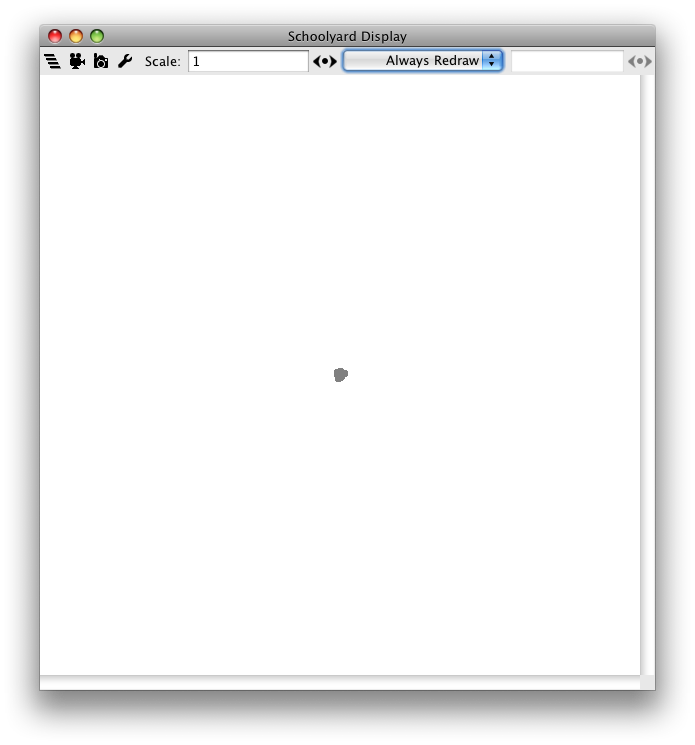
\includegraphics[width=3in]{Display2D.png}\vspace{-5em}\end{wrapfigure}

\paragraph{Compile and Run}  When we compile and run the code...

{\footnotesize \begin{alltt}
\textit{javac StudentsWithUI.java Students.java Student.java
java StudentsWithUI}
\end{alltt}}

Notice that we now have {\it two windows}:\footnote{You can have as many displays as you want.  Furthermore, you can have multiple displays for the same field; multiple fields shown in the same display; whatever you like.} the Console and a new Display2D window (actually a JFrame holding a Display2D within it).  The Display2D is shown at right.

At its default scaling, the Display2D shows the 100x100 region of the schoolyard.  You can see the children all clustered around the center of the schoolyard with a white background.  Press Play and you'll see them bouncing around in that tight cluster but never leaving (the force of the teacher is too strong).  We'll get them doing something more interesting in a moment.  But first, let's discuss some of the elements of the Display2D window:

\begin{itemize}
\item[\raisebox{-0.25em}{
\includegraphics[scale=0.4]{LayersButton.png}}] The Layers menu.  The Display2D overlays each field portrayal on top of one another.  This menu allows you to selectively display or hide various field portrayals (we only have one for now).
\item[\raisebox{-0.25em}{
\includegraphics[scale=0.4]{MovieButton.png}}] The Movie button.  Press this  to start a movie of the simulation running.
\item[\raisebox{-0.25em}{
\includegraphics[scale=0.4]{CameraButton.png}}] The Camera button.  Press this to take a picture of the simulation.  You can save the picture out as a bitmap (a PNG file) or as a publication-quality PDF vector image.
\item[\raisebox{-0.25em}{
\includegraphics[scale=0.4]{OptionsButton.png}}] The Options button.  Press this to bring up various drawing options.
\item[]\hspace{-1.5em}\raisebox{-0.25em}{
\includegraphics[scale=0.4]{ScaleField.png}}{\quad}The Scale Field.  This widget lets you zoom in and out of the display (change its scale).
\item[]\hspace{-1.5em}\raisebox{-0.25em}{
\includegraphics[scale=0.4]{RedrawField.png}}{\quad}The Redraw Field.  This widget lets you zoom in and out of the display (change its scale).
\end{itemize}

\section{Add a Social Network}

Right now the simulation isn't very interesting because the students are all huddled around the teacher.  Let's make them separate from one another based on how much they like or dislike one another.

We'll do this by adding a new field called a {\bf network}, defined by the class \Class{sim.field.network.Network}.  This class defines directed and undirected graphs and multigraphs\footnote{A {\it multigraph} is a graph where more than one edge can exist between two nodes.} with unlabeled, labeled, or weighted edges.

Network allows any object to be a node.  Objects are connected via edges defined by the class \Class{sim.field.network.Edge}.   An Edge stores an \variable{info} object which labels the edge: this can be anything.

Students will be embedded in an undirected graph, plus some random edges indicating strong like or dislike of one another.  If students lack an edge between them, we assume they have no mutual opinion.

Make the following changes to the \class{Students} class:

{\footnotesize \begin{alltt}
{\color{gray}import sim.engine.*;
import sim.util.*;
import sim.field.continuous.*;}
import sim.field.network.*;

{\color{gray}public class Students extends SimState
    \{
    public Continuous2D yard = new Continuous2D(1.0,100,100);
    public int numStudents = 50;
    double forceToSchoolMultiplier = 0.01;
    double randomMultiplier = 0.1;}
    public Network buddies = new Network(false);

    {\color{gray}public Students(long seed)
        \{
        super(seed);
        \}

    public void start()
        \{
        super.start();
        
        // clear the yard
        yard.clear();
        
        // clear the buddies
        buddies.clear();
        
        // add some students to the yard
        for(int i = 0; i < numStudents; i++)
            \{
            Student student = new Student();
            yard.setObjectLocation(student, 
                new Double2D(yard.getWidth() * 0.5 + random.nextDouble() - 0.5,
                    yard.getHeight() * 0.5 + random.nextDouble() - 0.5));}

            buddies.addNode(student);
            {\color{gray}schedule.scheduleRepeating(student);
            \}}
          
        // define like/dislike relationships
        Bag students = buddies.getAllNodes();
        for(int i = 0; i < students.size(); i++)
            \{
            Object student = students.get(i);
            
            // who does he like?
            Object studentB = null;
            do
                studentB = students.get(random.nextInt(students.numObjs));
            while (student == studentB);
            double buddiness = random.nextDouble();
            buddies.addEdge(student, studentB, new Double(buddiness));

            // who does he dislike?
            do
                studentB = students.get(random.nextInt(students.numObjs));
            while (student == studentB);
            buddiness = random.nextDouble();
            buddies.addEdge(student, studentB, new Double( -buddiness));
            \}
        \}
        
    {\color{gray}public static void main(String[] args)
        \{
        doLoop(Students.class, args);
        System.exit(0);
        \}
    \}}
\end{alltt}}

The first thing that the new code does is define a Network called \variable{buddies}.  This is the student relationships graph.  Notice that it's created with the parameter \variable{false}, indicating that it's an {\it undirected} graph.  Then each student is added to the graph as a node.

Afterwards the code adds random edges to this graph.  Each student likes at least one other student (not himself) and dislikes at least one other student (not himself).  It's possible for students to both like and dislike one another.

\sidebar{Why use a Bag?  Why not an ArrayList?}{Up until Java 1.6, Sun's ArrayList class has been {\it very slow}.  ArrayList's \method{get(...)}, \method{set(...)}, and \method{add(...)} methods have not been inlinable due to errors on Sun's part.  And of course, you can't access the underlying array directly.  We created Bag many years ago as a replacement for ArrayList with properly inlinable methods and with direct access to the array (if you're careful). This made Bag {\it much} faster than ArrayList.  Since extensible arrays are so common in simulation, and back-end simulation must be efficient, we felt it was an acceptable compromise to make: using a nonstandard class in return for an almost five-fold speedup.  It was a good decision for almost ten years.

Things have finally changed in Java 1.6.  Sun's HotSpot VM can now inline even methods like those in ArrayList.  This makes ArrayList decently fast.  So we may switch back to ArrayList at some time in the future if present trends continue.}%
Here's how the code works.  We first extract all the students from the graph with the method \method{getAllNodes()}.  This method returns a \Class{sim.util.Bag}, a faster replacement for Sun's \Class{java.util.ArrayList} which is used throughout MASON whenever speed is of importance.  Bag more or less has the same methods as ArrayList, so it shouldn't be hard to learn.

The \method{getAllNodes()} method returns a Bag used internally in Network, and which you should treat as {\bf read-only}: do not modify it.  If you want to modify it, make a copy and modify that.

The code does a loop through this bag of Students and, for each student, adds one random Edge for like and dislike respectively.  Each edge goes {\bf from} the student {\bf to} another student, and is {\bf weighted} with the degree of affinity (negative indicates dislike).  We pick the degree of affinity using the random number generator.

\paragraph{Have the Students Respond to the Network}  Now that the students have likes and dislikes, let's create a force that causes each Student to go towards the kids he likes and away from those he dislikes.

Here's how we'll do it for any given Student.  We create a temporary MutableDOuble2D called \variable{forceVector}, which folds the force from one student to another.  We then extract from the network all the edges connecting the Student to his buddies (those whom he likes or dislikes).

For each buddy, we grab the degree of affinity.  If the affinity is positive, then we create a force which draws the Student to the buddy.  If the affinity if negative, then we store in \variable{forceVector} a force which pushes the Student away from the buddy.  These forces are proportional to how close (or far away) the Student is from the buddy, like springs.  Finally, we add the force into the \variable{sumForces}.

Here's the edited \file{Student.java} file:

{\footnotesize \begin{alltt}
{\color{gray}import sim.engine.*;
import sim.field.continuous.*;
import sim.util.*;}
import sim.field.network.*;

{\color{gray}public class Student implements Steppable
    \{}
    public static final double MAX_FORCE = 3.0;

    {\color{gray}public void step(SimState state)
        \{
        Students students = (Students) state;
        Continuous2D yard = students.yard;

        Double2D me = students.yard.getObjectLocation(this);

        MutableDouble2D sumForces = new MutableDouble2D();}
                
        // Go through my buddies and determine how much I want to be near them
        MutableDouble2D forceVector = new MutableDouble2D();
        Bag out = students.buddies.getEdges(this, null);
        int len = out.size();
        for(int buddy = 0 ; buddy < len; buddy++)
            \{
            Edge e = (Edge)(out.get(buddy));
            double buddiness = ((Double)(e.info)).doubleValue();
            
            // I could be in the to() end or the from() end.  getOtherNode is a cute function
            // which grabs the guy at the opposite end from me.
            Double2D him = students.yard.getObjectLocation(e.getOtherNode(this));
            
            if (buddiness >= 0)  // the further I am from him the more I want to go to him
                \{
                forceVector.setTo((him.x - me.x) * buddiness, (him.y - me.y) * buddiness);
                if (forceVector.length() > MAX_FORCE)  // I'm far enough away
                    forceVector.resize(MAX_FORCE);
                \}
            else  // the nearer I am to him the more I want to get away from him, up to a limit
                \{
                forceVector.setTo((him.x - me.x) * buddiness, (him.y - me.y) * buddiness);
                if (forceVector.length() > MAX_FORCE)  // I'm far enough away
                    forceVector.resize(0.0);
                else if (forceVector.length() > 0)
                    forceVector.resize(MAX_FORCE - forceVector.length());  // invert the distance
                \}
            sumForces.addIn(forceVector);
            \}

        {\color{gray}// add in a vector to the "teacher" -- the center of the yard, so we don't go too far away
        sumForces.addIn(new Double2D((yard.width * 0.5 - me.x) * students.forceToSchoolMultiplier, 
                (yard.height * 0.5 - me.y) * students.forceToSchoolMultiplier));
        
        // add a bit of randomness
        sumForces.addIn(new Double2D(students.randomMultiplier * (students.random.nextDouble() * 1.0 - 0.5), 
                students.randomMultiplier * (students.random.nextDouble() * 1.0 - 0.5)));

        sumForces.addIn(me);

        students.yard.setObjectLocation(this, new Double2D(sumForces));
        \}
    \}} 
\end{alltt}}


\bump

\begin{wrapfigure}{r}[0in]{3in}
\vspace{-2em}\hfill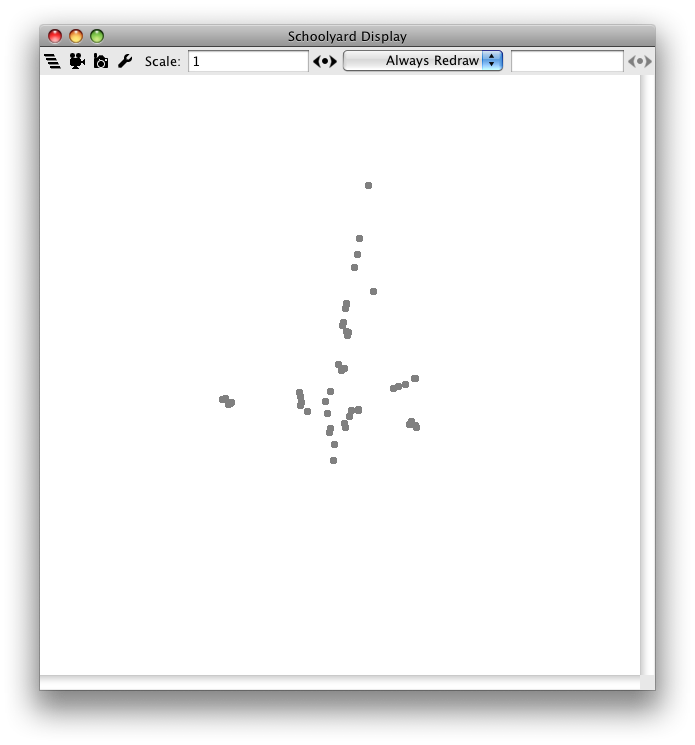
\includegraphics[width=3in]{Schoolyard1.png}\vspace{-5em}\end{wrapfigure}

Notice the various MutableDouble2D convenience methods being used. First there's the \method{setTo(...)} method: this simply replaces the X and Y values in the MutableDouble2D with the given values.  Next, there's the \method{length()} method, which returns \(\sqrt{X^2 + Y^2}\).  And the method \method{resize(...)} scales X and Y so that \(\sqrt{X^2 + Y^2} = L\) for the desired length \(L\).   There are a lot more than that.  These methods are just for convenience of course: you can just set the X and Y values yourself.

\paragraph{Compile and Run}  If you compile and run the simulation at this point...

{\footnotesize \begin{alltt}
\textit{javac StudentsWithUI.java Students.java Student.java
java StudentsWithUI}
\end{alltt}}

\noindent ...you'll find that the students now push away from one another, settling into lines of affinity.  But we can't see the network yet, nor visualize the strain it's putting on the students.  We'll do that next.

\section{Visualize the Social Network}

Visualizing a Network is easy, since we're already drawing the nodes (the Students).  We merely have to set up a \Class{sim.portrayal.network.NetworkPortrayal2D} and tell it two things:

\begin{itemize}
\item What Network it should be portraying (this tells it which edges to draw).
\item What Continuous2D or other spatial field is associating the nodes (in our case, the Students) with locations.  This tells it {\it where} to draw the edges.
\end{itemize}

A NetworkPortrayal2D, like all field portrayals, is assigned a field to draw via the method \method{setField(...)}.  Since the NetworkPortrayal2D in actuality needs {\it two} fields, we create a special ``field'' of sorts which stores both of them and pass that in instead.  That object is called a \Class{sim.portrayal.network.SpatialNetwork2D}.

The nodes are already being drawn: we simply need to define how to portray the edges.  We'll do this by assigning a \Class{sim.portrayal.network.SimpleEdgePortrayal2D}, which just draws them as black lines.\footnote{You can change the color if you like.  And for directed edges, you can choose the color of the ``from'' portion of the edge and the color of the ``to'' portion of the edge to distinguish them.  There are other non-line options as well.  And yes, you can draw the labels or weights.}

We edit the \file{StudentsWithUI.java} file.  The changes are pretty small:

{\footnotesize \begin{alltt}
import sim.portrayal.network.*;
{\color{gray}import sim.portrayal.continuous.*;
import sim.engine.*;
import sim.display.*;
import sim.portrayal.simple.*;
import javax.swing.*;
import java.awt.Color;


public class StudentsWithUI extends GUIState
    \{
    public Display2D display;
    public JFrame displayFrame;

    ContinuousPortrayal2D yardPortrayal = new ContinuousPortrayal2D();}
    NetworkPortrayal2D buddiesPortrayal = new NetworkPortrayal2D();

    {\color{gray}public static void main(String[] args)
        \{
        StudentsWithUI vid = new StudentsWithUI();
        Console c = new Console(vid);
        c.setVisible(true);
        \}

    public StudentsWithUI() \{ super(new Students( System.currentTimeMillis())); \}
    public StudentsWithUI(SimState state) \{ super(state); \}

    public static String getName() \{ return "Student Schoolyard Cliques";  \}
    
    public void start()
        \{
        super.start();
        setupPortrayals();
        \}

    public void load(SimState state)
        \{
        super.load(state);
        setupPortrayals();
        \}

    public void setupPortrayals()
        \{
        Students students = (Students) state;
        
        // tell the portrayals what to portray and how to portray them
        yardPortrayal.setField( students.yard );
        yardPortrayal.setPortrayalForAll(new OvalPortrayal2D());}
        
        buddiesPortrayal.setField( new SpatialNetwork2D( students.yard, students.buddies ) );
        buddiesPortrayal.setPortrayalForAll(new SimpleEdgePortrayal2D());

        {\color{gray}// reschedule the displayer
        display.reset();
        display.setBackdrop(Color.white);

        // redraw the display
        display.repaint();
        \}

    public void init(Controller c)
        \{
        super.init(c);

        // make the displayer
        display = new Display2D(600,600,this);
        // turn off clipping
        display.setClipping(false);

        displayFrame = display.createFrame();
        displayFrame.setTitle("Schoolyard Display");
        c.registerFrame(displayFrame);   // register the frame so it appears in the "Display" list
        displayFrame.setVisible(true);}
        display.attach( buddiesPortrayal, "Buddies" );
        {\color{gray}display.attach( yardPortrayal, "Yard" );
        \}

    public void quit()
        \{
        super.quit();

        if (displayFrame!=null) displayFrame.dispose();
        displayFrame = null;
        display = null;
        \}
    \}}
\end{alltt}}


\begin{wrapfigure}{r}[0in]{3in}
\vspace{-15em}\hfill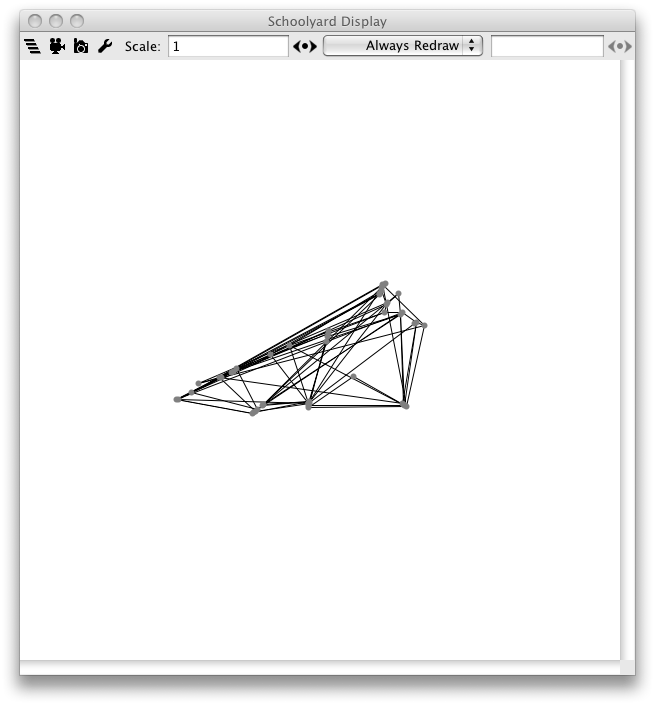
\includegraphics[width=3in]{Schoolyard2.png}\vspace{-5em}\end{wrapfigure}

\paragraph{Compile and Run}  And we're off and running!

{\footnotesize \begin{alltt}
\textit{javac StudentsWithUI.java Students.java Student.java
java StudentsWithUI}
\end{alltt}}

As shown at right, we've now got edges being drawn.  Now let's modify how the nodes are drawn to reflect how agitated the students are.


\section{Inspect Student Agitation and Customize its Visualizaion}

Before we can visualize how agitated the students are, we'll need to actually define what ``agitated'' means.  We'll define it in terms of the affinity forces: a student is happier if he has lower affinity forces on him (he's fine where he is), and more agitated if the forces are high.

Modify the file \file{Student.java}:

{\footnotesize \begin{alltt}
{\color{gray}import sim.engine.*;
import sim.field.continuous.*;
import sim.util.*;
import sim.field.network.*;

public class Student implements Steppable
    \{
    public static final double MAX_FORCE = 3.0;}
    
    double friendsClose = 0.0;  // initially very close to my friends
    double enemiesCloser = 10.0;  // WAY too close to my enemies
    public double getAgitation() \{ return friendsClose + enemiesCloser; \}

    {\color{gray}public void step(SimState state)
        \{
        Students students = (Students) state;
        Continuous2D yard = students.yard;

        Double2D me = students.yard.getObjectLocation(this);

        MutableDouble2D sumForces = new MutableDouble2D();}
        
        friendsClose = enemiesCloser = 0.0;
        
        {\color{gray}// Go through my buddies and determine how much I want to be near them
        MutableDouble2D forceVector = new MutableDouble2D();
        Bag out = students.buddies.getEdges(this, null);
        int len = out.size();
        for(int buddy = 0 ; buddy < len; buddy++)
            \{
            Edge e = (Edge)(out.get(buddy));
            double buddiness = ((Double)(e.info)).doubleValue();
            
            // I could be in the to() end or the from() end.  getOtherNode is a cute function
            // which grabs the guy at the opposite end from me.
            Double2D him = students.yard.getObjectLocation(e.getOtherNode(this));
            
            if (buddiness >= 0)  // the further I am from him the more I want to go to him
                \{
                forceVector.setTo((him.x - me.x) * buddiness, (him.y - me.y) * buddiness);
                if (forceVector.length() > MAX_FORCE)  // I'm far enough away
                    forceVector.resize(MAX_FORCE);}
                friendsClose += forceVector.length();
                {\color{gray}\}
            else  // the nearer I am to him the more I want to get away from him, up to a limit
                \{
                forceVector.setTo((him.x - me.x) * buddiness, (him.y - me.y) * buddiness);
                if (forceVector.length() > MAX_FORCE)  // I'm far enough away
                    forceVector.resize(0.0);
                else if (forceVector.length() > 0)
                    forceVector.resize(MAX_FORCE - forceVector.length());  // invert the distance}
                enemiesCloser += forceVector.length();
                {\color{gray}\}
            sumForces.addIn(forceVector);}
           {\color{gray}\}

        // add in a vector to the "teacher" -- the center of the yard, so we don't go too far away
        sumForces.addIn(new Double2D((yard.width * 0.5 - me.x) * students.forceToSchoolMultiplier, 
                (yard.height * 0.5 - me.y) * students.forceToSchoolMultiplier));
        
        // add a bit of randomness
        sumForces.addIn(new Double2D(students.randomMultiplier * (students.random.nextDouble() * 1.0 - 0.5), 
                students.randomMultiplier * (students.random.nextDouble() * 1.0 - 0.5)));

        sumForces.addIn(me);
        
        students.yard.setObjectLocation(this, new Double2D(sumForces));
        \}
    \}}
\end{alltt}}

Notice that we've set up this value (\variable{agitation}) as a read-only Java Bean Property via the method \method{getAgitation()}.  This will come in handy later.

Notice also that the initial size of the variable \variable{enemiesCloser} is 10.0, not 0.0.  There's a reason for this.  When the students exit the schoolyard, they're very close to their enemies; but this isn't reflected in the very first frame of the simulation visualization, because the \method{step(...)} method hasn't been called yet.  So they all will look initially very happy.  We remedy this by making them initially very agitated at step 0!

\paragraph{Change Student Color}

Now let's customize the color of the student to reflect their degree of agitation.  You can portray the students in any way you like: just create your own \Class{sim.portrayal.SimplePortrayal2D} subclass; or have the Students themselves subclass from SimplePortrayal2D.  But you could also take an existing SimplePortrayal2D and modify it: typically change its size or its color.  We'll do that.

Recall that our students are presently being portrayed as gray circles using the SimplePortrayal2D subclass \Class{sim.portrayal.simple.OvalPortrayal2D}.  This class has three variables you can customize:  \variable{Paint paint} (the color), \variable{double scale} (the size), and \variable{boolean filled}.  We could just set the color and be done with it, but to have the color dynamically change each step, we'll need to override the method \method{draw(...)} to change the color to the proper value, then call \code{super.draw(...)} to draw the oval.

You can make a custom subclass in its own file, but it's just simpler to use an anonymous subclass:

{\footnotesize \begin{alltt}
{\color{gray}import sim.portrayal.network.*;
import sim.portrayal.continuous.*;
import sim.engine.*;
import sim.display.*;
import sim.portrayal.simple.*;}
import sim.portrayal.*;
{\color{gray}import javax.swing.*;
import java.awt.Color;}
import java.awt.*;

{\color{gray}public class StudentsWithUI extends GUIState
    \{
    public Display2D display;
    public JFrame displayFrame;

    ContinuousPortrayal2D yardPortrayal = new ContinuousPortrayal2D();
    NetworkPortrayal2D buddiesPortrayal = new NetworkPortrayal2D();

    public static void main(String[] args)
        \{
        StudentsWithUI vid = new StudentsWithUI();
        Console c = new Console(vid);
        c.setVisible(true);
        \}

    public StudentsWithUI() \{ super(new Students( System.currentTimeMillis())); \}
    public StudentsWithUI(SimState state) \{ super(state); \}

    public static String getName() \{ return "Student Schoolyard Cliques";  \}
    
    public void start()
        \{
        super.start();
        setupPortrayals();
        \}

    public void load(SimState state)
        \{
        super.load(state);
        setupPortrayals();
        \}

    public void setupPortrayals()
        \{
        Students students = (Students) state;
        
        // tell the portrayals what to portray and how to portray them
        yardPortrayal.setField( students.yard );
        yardPortrayal.setPortrayalForAll(new OvalPortrayal2D()}
            \{
            public void draw(Object object, Graphics2D graphics, DrawInfo2D info)
                \{
                Student student = (Student)object;

                int agitationShade = (int) (student.getAgitation() * 255 / 10.0);
                if (agitationShade > 255) agitationShade = 255;
                paint = new Color(agitationShade, 0, 255 - agitationShade);
                super.draw(object, graphics, info);
                \}
            \}{\color{gray});
        
        buddiesPortrayal.setField( new SpatialNetwork2D( students.yard, students.buddies ) );
        buddiesPortrayal.setPortrayalForAll(new SimpleEdgePortrayal2D());

        // reschedule the displayer
        display.reset();
        display.setBackdrop(Color.white);

        // redraw the display
        display.repaint();
        \}

    public void init(Controller c)
        \{
        super.init(c);

        // make the displayer
        display = new Display2D(600,600,this);
        // turn off clipping
        display.setClipping(false);

        displayFrame = display.createFrame();
        displayFrame.setTitle("Schoolyard Display");
        c.registerFrame(displayFrame);   // register the frame so it appears in the "Display" list
        displayFrame.setVisible(true);
        display.attach( buddiesPortrayal, "Buddies" );
        display.attach( yardPortrayal, "Yard" );
        \}

    public void quit()
        \{
        super.quit();

        if (displayFrame!=null) displayFrame.dispose();
        displayFrame = null;
        display = null;
        \}
    \}}
\end{alltt}}

\begin{wrapfigure}{r}[0in]{3in}
\vspace{-3em}\hfill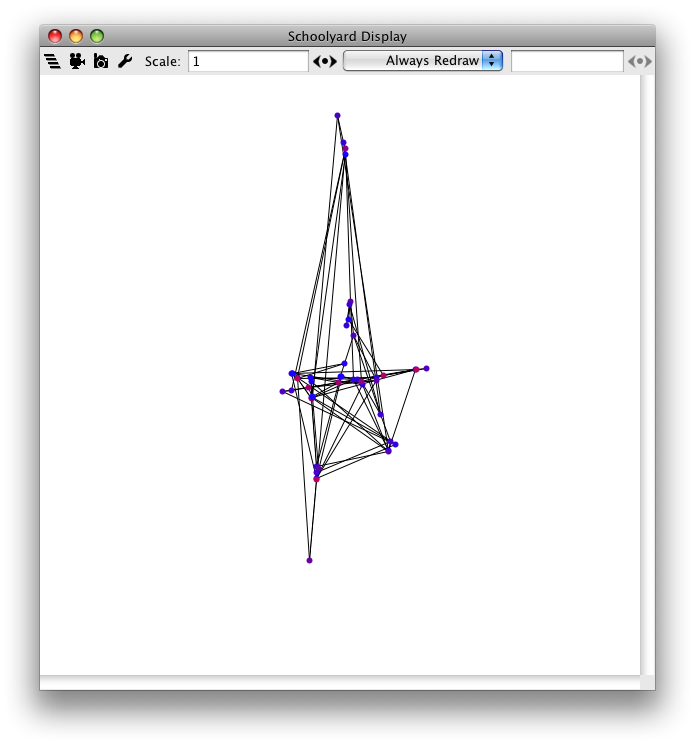
\includegraphics[width=3in]{Schoolyard3.png}\vspace{-5em}\end{wrapfigure}

Note that the \method{draw(...)} method is passed the object to draw (a Student).  From this we extract the agitation, then set an appropriate Color (ranging from red to blue). Finally (and crucially) we call \method{super.draw(...)} to draw the Student.

\paragraph{Compile and Run}

{\footnotesize \begin{alltt}
\textit{javac StudentsWithUI.java Students.java Student.java
java StudentsWithUI}
\end{alltt}}

As you can see at right, we now have students at various levels of agitation.  As students head away from one another, they'll get less agitated, but some students seem to be unhappy no matter where they are.

\paragraph{Inspect}

Now that our students have certain Java Bean Properties, we can inspect those values in various ways.  For example, we can:

\begin{itemize}
\item Examine the values (and modify them if the Properties are writable, which isn't the case in this example).
\item Track properties on a time series chart or a histogram.
\item Write the properties out to a file or to a text window.
\end{itemize}

\begin{wrapfigure}{r}[0in]{3in}
\vspace{-12.5em}\hfill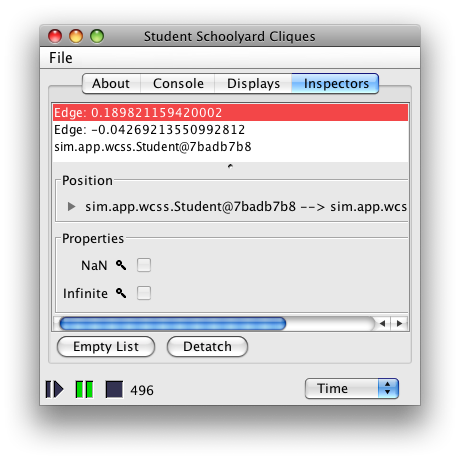
\includegraphics[width=2.8in]{ConsoleInspectors.png}\vspace{-3em}\end{wrapfigure}


It's easy to to inspect a Student now.  Double-click on a student and the Console will shift to showing a list of Inspectors, one for each object you hit with the mouse.  If you find it challenging to select a student, try rescaling the simulation a bit via the Scale Field \raisebox{-0.25em}{
\includegraphics[scale=0.4]{ScaleField.png}},

The two things inspectable in the simulation, at the moment, are Students and Edges.  At right is the Console after I clicked on a particularly simple Student with just two Edges.  Often you'll get a bounty of Edges, followed by one or a few Students, depending on what you clicked on.

\begin{wrapfigure}{r}[0in]{3in}
\vspace{-1em}\hfill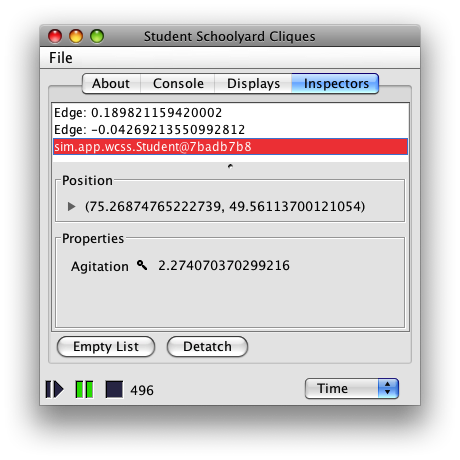
\includegraphics[width=2.8in]{ConsoleInspectors2.png}\vspace{-2em}\end{wrapfigure}


In the Console at right we see the list of Inspectors, and beneath it the \Class{sim.portrayal.SimpleInspector} for an Edge with weight 0.18921159420002.\footnote{Actually, it's {\it two} inspectors one nested in the other: the SimpleInspector is displaying the stuff inside the ``Properties'' box.  The ContinuousPortrayal2D wrapped this in an outer Inspector which also includes the position of the object.  Also if you look carefully you'll see the Students are called \class{sim.app.wcss.Student} rather than just \class{Student}: I took these screenshots from the WCSS tutorial.  So sue me.}   An Inspector (usually a SimpleInspector) is produced by the SimplePortrayal2D (in this case, the OvalPortrayal2D) when requested by the Display2D after the user double-clicked on an object.  Notice that the Edge has two properties: \textit{NaN} and \textit{Infinite}.  The Edge is displaying a SimpleInspector for its \variable{info} object, and we placed a \Class{java.lang.Double} in there (that's what's holding the 0.18921159420002 value).  Sun's Double class has two unhelpful Java Bean Property methods: \method{isNaN()} and \method{isInfinite()}.  

Click on the Student\footnote{Don't like that ugly name for the Student in the Inspector list?  Override the Student's \method{toString()} method, and it'll be used instead.} and you'll get an Inspector like the one shown at right.  The Student has one property: \textit{Agitation}.  This corresponds to the Java Bean Property Method we defined: \method{getAgitation()}.  If you continue the simulation, you'll find that this property automatically updates.\footnote{Also the simulation runs more slowly because there's more stuff to draw on-screen.  Click ``Empty List'' to get rid of the Inspectors and make the simulation run faster.  You can make the simulation run even faster by getting rid of the display.  Click the display's close box (on OS X, the red button).  Last, change the Time Button \raisebox{-0.25em}{
\includegraphics[scale=0.4]{TimeButton.png}} to say ``Rate'', which is updated less often.  With no displays to draw, no inspectors to update, and no steps counter to repaint, the GUI will approach\,---\,but not match\,---\,the speed you get if you just run on the command line.  Don't worry, you can get the display back -- go to the Displays tab \raisebox{-0.25em}{
\includegraphics[scale=0.4]{DisplaysButton.png}} and double-click on the display.}

We can go further than this.  Let's chart the degree of agitation of a given Student.  Stop the simulation and start it paused (click on the Pause button \raisebox{-0.25em}{
\includegraphics[scale=0.4]{PauseButton.png}} when the console is Stopped \raisebox{-0.25em}{
\includegraphics[scale=0.4]{StopButton.png}}\ ).  Then step the simulation a few times and double-click on a student and inspect it.  Next, click on the magnifying glass button \raisebox{-0.2em}{
\includegraphics[scale=0.4]{MagnifyingGlassButton.png}} next to the \textit{Agitation} property.  Up will pop up a menu which lets you {\it stream} the property to a file or to a window, or {\it chart} the property\footnote{MASON uses the charting library {\it JFreeChart} (http:/\!/jfree.org/jfreechart/) to do charting in its inspectors.} by calling forth further inspectors to do more interesting things.

\begin{wrapfigure}{r}[0in]{3.8in}
\vspace{-1em}\hfill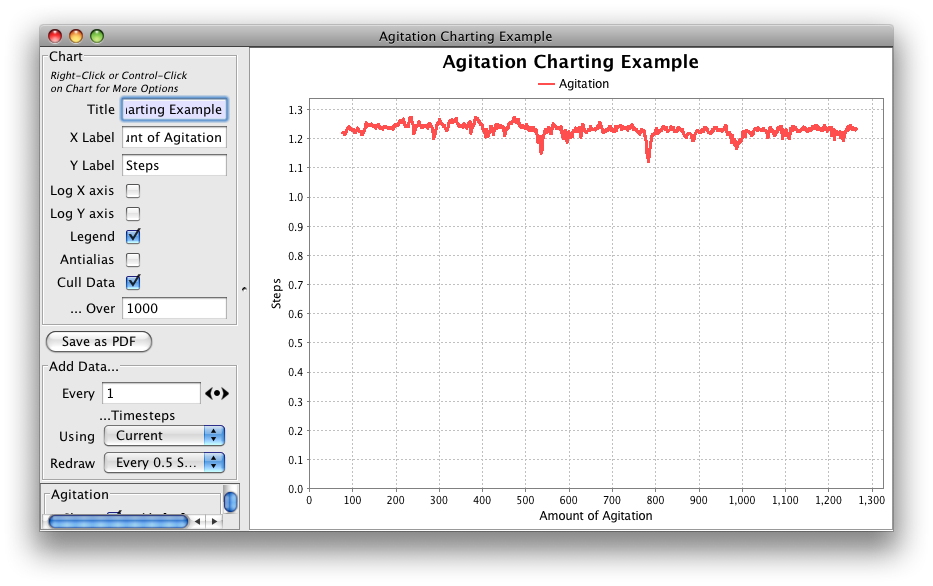
\includegraphics[width=4in]{Chart.png}\vspace{-2em}\end{wrapfigure}


These inspectors are different from the SimpleInspectors you've seen so far. SimpleInspector is designed to inspect an {\it object}.  These additional inspectors, subclasses of \Class{sim.portrayal.inspector.PropertyInspector}, are designed to inspect {\it the value of a property of an object}.  Second, PropertyInspectors can be dynamically plugged-in at run-time, and appear in that pop-up menu.

Select {\it Chart} from the pop-up menu and you'll get a chart window like the one at right.  Make some tweaks of features, unpause the simulation, and watch the chart unspool.  If you click on ``Save as PDF...'', you can generate a publication-quality PDF output of the chart (as opposed to a bitmap screenshot).

\section{Inspect the Model} 

Let's add an inspector for the global model parameters.  Before we do so, it might be useful to {\it have} global model parameters!  So we'll modify the \file{Students.java} file, adding some Java Bean Properties.  We add four properties below, and they all have interesting features which need to be explained:

\begin{itemize}
\item \method {getNumStudents()} is accompanied by \method{setNumStudents(...)}.  This makes it a read-write property, not just a read-only property.  As a result you'll be able to change the number of students in the Inspector (via a text field), not just view it.
\item Likewise, \method{getForceToSchoolMultiplier()} is accompanied by \method{setForceToSchoolMultiplier(...)}, making it a read-write property.
\item \method{getRandomMultiplier()} is not only accompanied by \method{setRandomMultiplier(...)}, making it a read-write property, but it's also accompanied by a special method name custom to MASON: \method{domRandomMultipler()}.  If a property {\it Foo} has a method called \method{domFoo()}, MASON interprets this as providing the {\it domain} of the property.  There are two domains recognized: either a \Class{sim.util.Interval}, which defines the legal range of a numerical property; or an array of Strings. In the first place, MASON replaces the standard read-write text field with a slider.  In the second case, MASON replaced the text field with a pop-up menu of those Strings.  If you choose a String, then the property is set to the index value of the String in the array (starting at 0).
\item \method{getAgitationDistribution()} is computed at runtime.  Furthermore it doesn't return a simple integer or boolean value: it returns an {\it array of doubles}.  Arrays or lists of objects allow you to create historgrams as property inspectors.
\end{itemize}

Here's the code.

{\footnotesize \begin{alltt}
{\color{gray}import sim.engine.*;
import sim.util.*;
import sim.field.continuous.*;
import sim.field.network.*;

public class Students extends SimState
    \{
    public Continuous2D yard = new Continuous2D(1.0,100,100);
    
    public int numStudents = 50;

    double forceToSchoolMultiplier = 0.01;
    double randomMultiplier = 0.1;}

    public int getNumStudents() \{ return numStudents; \}
    public void setNumStudents(int val) \{ if (val > 0) numStudents = val; \}

    public double getForceToSchoolMultiplier() \{ return forceToSchoolMultiplier; \}
    public void setForceToSchoolMultiplier(double val)
        \{ if (forceToSchoolMultiplier >= 0.0) forceToSchoolMultiplier = val; \}

    public double getRandomMultiplier() \{ return randomMultiplier; \}
    public void setRandomMultiplier(double val) \{ if (randomMultiplier >= 0.0) randomMultiplier = val; \}
    public Object domRandomMultiplier() \{ return new sim.util.Interval(0.0, 100.0); \}

    public double[] getAgitationDistribution()
        \{
        Bag students = buddies.getAllNodes();
        double[] distro = new double[students.numObjs];
        for(int i = 0; i < students.numObjs; i++)
            distro[i] = ((Student)(students.objs[i])).getAgitation();
        return distro;
        \}

    {\color{gray}public Network buddies = new Network(false);

    public Students(long seed)
        \{
        super(seed);
        \}

    public void start()
        \{
        super.start();
        
        // clear the yard
        yard.clear();

        // clear the buddies
        buddies.clear();
        
        // add some students to the yard
        for(int i = 0; i < numStudents; i++)
            \{
            Student student = new Student();
            yard.setObjectLocation(student, 
                new Double2D(yard.getWidth() * 0.5 + random.nextDouble() - 0.5,
                    yard.getHeight() * 0.5 + random.nextDouble() - 0.5));

            buddies.addNode(student);
            schedule.scheduleRepeating(student);
            \}
        
        // define like/dislike relationships
        Bag students = buddies.getAllNodes();
        for(int i = 0; i < students.size(); i++)
            \{
            Object student = students.get(i);
            
            // who does he like?
            Object studentB = null;
            do
                \{
                studentB = students.get(random.nextInt(students.numObjs));
                \} while (student == studentB);
            double buddiness = random.nextDouble();
            buddies.addEdge(student, studentB, new Double(buddiness));

            // who does he dislike?
            do
                \{
                studentB = students.get(random.nextInt(students.numObjs));
                \} while (student == studentB);
            buddiness = random.nextDouble();
            buddies.addEdge(student, studentB, new Double( -buddiness));
            \}
        \}
        
    public static void main(String[] args)
        \{
        doLoop(Students.class, args);
        System.exit(0);
        \}    
    \}}
\end{alltt}}

We also need to modify the file \file{StudentsWithUI.java} to inform MASON that it should display an Inspector for the model.  We need to actually tell it two things:

\begin{itemize}
\item The object from which it should extract the Java Bean Properties.  Typically this is the model (SimState subclass) itself.  To do this we add a single method called \method{getSimulationInspectedObject()}.
\item That the Inspector is {\it volatile} and thus must be updated every timestep.  This is expensive, and not all that common (usually we use model inspectors to set parameters at the beginning of a run).  But in this example, our Inspector will be providing data such as histogram information which changes each timestep.  So we need to declare it to be volatile.  To do this we override the method \method{getInspector()} to set the inspector to be volatile before returning it.
\end{itemize}

Here's the code, it's pretty straightforward:

{\footnotesize \begin{alltt}
{\color{gray}import sim.portrayal.network.*;
import sim.portrayal.continuous.*;
import sim.engine.*;
import sim.display.*;
import sim.portrayal.simple.*;
import sim.portrayal.*;
import javax.swing.*;
import java.awt.Color;
import java.awt.*;

public class StudentsWithUI extends GUIState
    \{
    public Display2D display;
    public JFrame displayFrame;

    ContinuousPortrayal2D yardPortrayal = new ContinuousPortrayal2D();
    NetworkPortrayal2D buddiesPortrayal = new NetworkPortrayal2D();

    public static void main(String[] args)
        \{
        StudentsWithUI vid = new StudentsWithUI();
        Console c = new Console(vid);
        c.setVisible(true);
        \}

    public StudentsWithUI() \{ super(new Students( System.currentTimeMillis())); \}
    public StudentsWithUI(SimState state) \{ super(state); \}

    public static String getName() \{ return "Student Schoolyard Cliques";  \}}
    
    public Object getSimulationInspectedObject() \{ return state; \}

    public Inspector getInspector()
        \{
        Inspector i = super.getInspector();
        i.setVolatile(true);
        return i;
        \}

    {\color{gray}public void start()
        \{
        super.start();
        setupPortrayals();
        \}

    public void load(SimState state)
        \{
        super.load(state);
        setupPortrayals();
        \}

    public void setupPortrayals()
        \{
        Students students = (Students) state;
        
        // tell the portrayals what to portray and how to portray them
        yardPortrayal.setField( students.yard );
        yardPortrayal.setPortrayalForAll(new OvalPortrayal2D()
            \{
            public void draw(Object object, Graphics2D graphics, DrawInfo2D info)
                \{
                Student student = (Student)object;

                int agitationShade = (int) (student.getAgitation() * 255 / 10.0);
                if (agitationShade > 255) agitationShade = 255;
                paint = new Color(agitationShade, 0, 255 - agitationShade);
                super.draw(object, graphics, info);
                \}
            \});
        
        buddiesPortrayal.setField( new SpatialNetwork2D( students.yard, students.buddies ) );
        buddiesPortrayal.setPortrayalForAll(new SimpleEdgePortrayal2D());

        // reschedule the displayer
        display.reset();
        display.setBackdrop(Color.white);

        // redraw the display
        display.repaint();
        \}

    public void init(Controller c)
        \{
        super.init(c);

        // make the displayer
        display = new Display2D(600,600,this);
        // turn off clipping
        display.setClipping(false);

        displayFrame = display.createFrame();
        displayFrame.setTitle("Schoolyard Display");
        c.registerFrame(displayFrame);   // register the frame so it appears in the "Display" list
        displayFrame.setVisible(true);
        display.attach( buddiesPortrayal, "Buddies" );
        display.attach( yardPortrayal, "Yard" );
        \}

    public void quit()
        \{
        super.quit();

        if (displayFrame!=null) displayFrame.dispose();
        displayFrame = null;
        display = null;
        \}
    \}}
\end{alltt}}

\bump

\paragraph{Compile and Run}

{\footnotesize \begin{alltt}
\textit{javac StudentsWithUI.java Students.java Student.java
java StudentsWithUI}
\end{alltt}}

\begin{wrapfigure}{r}[0in]{3in}
\vspace{-8em}\hfill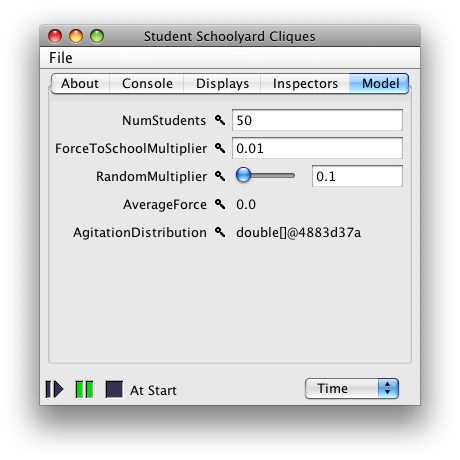
\includegraphics[width=2.8in]{ConsoleInspectors3.png}\vspace{-5em}\end{wrapfigure}

When you fire up MASON this time, notice that the Console now has an extra tab at the end: the {\bf Model Tab} \raisebox{-0.25em}{
\includegraphics[scale=0.4]{ModelButton.png}}. This tab reveals the Model's Inspector, as shown at right.  Notice the five properties we added, one of which has a slider.

\paragraph{Important Note} The Model Inspector isn't valid until you start the simulation.  So examining or setting values when the Simulation is Stopped  \raisebox{-0.25em}{
\includegraphics[scale=0.4]{StopButton.png}} may have no effect.  Instead, press Pause \raisebox{-0.25em}{
\includegraphics[scale=0.4]{PauseButton.png}} first, then modify and examine the inspector.

\begin{wrapfigure}{r}[0in]{4in}
\vspace{-1em}\hfill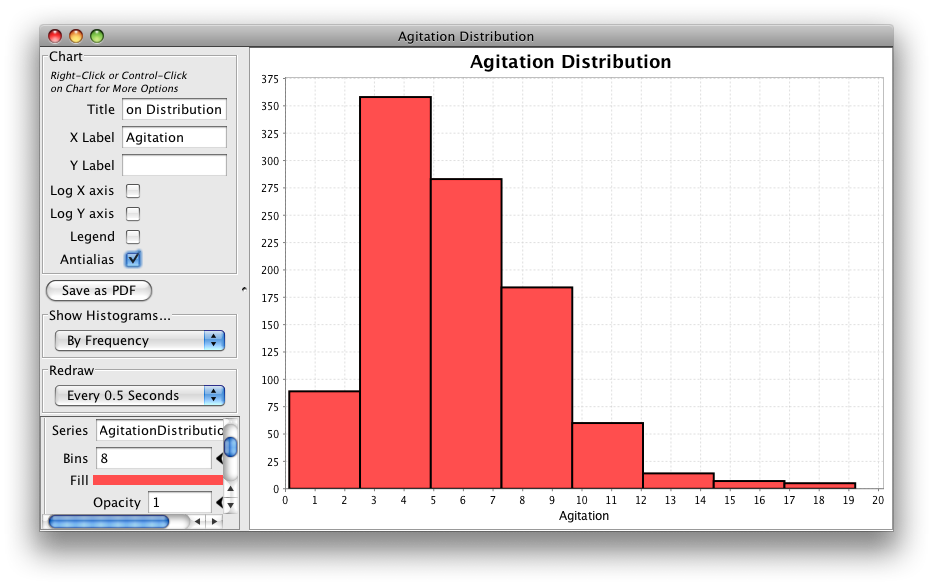
\includegraphics[width=4in]{Histogram.png}\vspace{-1em}\end{wrapfigure}

Try tweaking these values.  Note that you can only modify the number of students before starting a simulation (the model uses this value at \method{start(...)} time and nowhere else) but the two Multiplier properties can be modified whenever you like.  Try setting the number of students to 1000 for example.  Or change the degree of randomness.

You can create time series charts from the {\it AverageForce} property.  But more interesting, you can now create histograms of from the double array generated by \method{getAgitationDistribution()}.  Just click on the magnifying glass button \raisebox{-0.2em}{
\includegraphics[scale=0.4]{MagnifyingGlassButton.png}} and select {\it Histogram}.  Up pops a histogram like the one here.

\sidebar{Can you have more than one series on a chart?}{Absolutely. Histograms and time series charts both support multiple series.  Just ask to chart a second item, and you'll be given the option to put it on its own chart or to add it to an existing chart.}


\section{Select, Label, and Move Students} 

MASON allows you to {\it select} objects with the mouse, which signals further state changes in those objects; and to {\it move} objects by dragging them.  Selecting happens automatically, but there's no effect unless you add something which responds to the selection.  Moving is not enabled by default at all, so we'll do it here.

Let's start with selection.

MASON has a concept called {\bf wrapper portrayals}, which are special SimplePortrayals which contain nested SimplePortrayals (the primary portrayals) within them.  A wrapper portrayal adds additional functionality beyond what the SimplePortrayal provides.  You can have as many wrapper portrayals wrapped around your SimplePortrayal as you like.  Here are some wrapper portrayals available:

\begin{itemize}
\item \Class{sim.portrayal.simple.CircledPortrayal2D} draws a circle around the object to hilight it.  CircledPortrayals can be set to to only draw the circle when the object is selected (or always draw it).
\item \Class{sim.portrayal.simple.LabelledPortrayal2D} adds a text label the object.  LabelledPortrayals can be set to to only add the label when the object is selected (or always draw it).  LabelledPortrayals can have a fixed label or one based on some value of the object which changes as you like.
\item \Class{sim.portrayal.simple.FacetedPortrayal2D} has more than one subsidiary SimplePortrayal, and changes which SimplePortrayal is in charge based on the current state of the object.  Particularly useful for doing simple animations.
\item \Class{sim.portrayal.simple.MovablePortrayal2D} allows you to drag and move the object.
\item \Class{sim.portrayal.simple.OrientedPortrayal2D} adds an orientation marker to the object to demonstrate what ``direction'' it's ``pointing''.
\item \Class{sim.portrayal.simple.TrailedPortrayal2D} adds a fading-out trail to the object so you can see the route it's taken.
\item \Class{sim.portrayal.simple.TransformedPortrayal2D} scales, rotates, or translates the object with respect to the underlying portrayal.
\end{itemize}

Notice the theme?  All wrapper portrayal names are adjectives like ``circled'' or ``movable'' or ``transformed''. 

In the code below we wrap the OvalPortrayal2D in not one, not two, but {\it three} wrapper portrayals: MovablePortrayal2D,  CircledPortrayal2D, and LabelledPortrayal2D. It's easy:

{\footnotesize \begin{alltt}
{\color{gray}import sim.portrayal.network.*;
import sim.portrayal.continuous.*;
import sim.engine.*;
import sim.display.*;
import sim.portrayal.simple.*;
import sim.portrayal.*;
import javax.swing.*;
import java.awt.Color;
import java.awt.*;

public class StudentsWithUI extends GUIState
    \{
    public Display2D display;
    public JFrame displayFrame;

    ContinuousPortrayal2D yardPortrayal = new ContinuousPortrayal2D();
    NetworkPortrayal2D buddiesPortrayal = new NetworkPortrayal2D();

    public static void main(String[] args)
        \{
        StudentsWithUI vid = new StudentsWithUI();
        Console c = new Console(vid);
        c.setVisible(true);
        \}

    public StudentsWithUI() \{ super(new Students( System.currentTimeMillis())); \}
    public StudentsWithUI(SimState state) \{ super(state); \}

    public static String getName() \{ return "Student Schoolyard Cliques";  \}
    
    public Object getSimulationInspectedObject() \{ return state; \}

    public Inspector getInspector()
        \{
        Inspector i = super.getInspector();
        i.setVolatile(true);
        return i;
        \}

    public void start()
        \{
        super.start();
        setupPortrayals();
        \}

    public void load(SimState state)
        \{
        super.load(state);
        setupPortrayals();
        \}

    public void setupPortrayals()
        \{
        Students students = (Students) state;
        
        // tell the portrayals what to portray and how to portray them
        yardPortrayal.setField( students.yard );
        yardPortrayal.setPortrayalForAll(}
            new MovablePortrayal2D(
                new CircledPortrayal2D(
                    new LabelledPortrayal2D(
                        {\color{gray}new OvalPortrayal2D()
                            \{
                            public void draw(Object object, Graphics2D graphics, DrawInfo2D info)
                                \{
                                Student student = (Student)object;

                                int agitationShade = (int) (student.getAgitation() * 255 / 10.0);
                                if (agitationShade > 255) agitationShade = 255;
                               paint = new Color(agitationShade, 0, 255 - agitationShade);
                                super.draw(object, graphics, info);
                                \}
                            \}}, 
                        5.0, null, Color.black, true),
                    0, 5.0, Color.green, true)){\color{gray});
        
        buddiesPortrayal.setField( new SpatialNetwork2D( students.yard, students.buddies ) );
        buddiesPortrayal.setPortrayalForAll(new SimpleEdgePortrayal2D());

        // reschedule the displayer
        display.reset();
        display.setBackdrop(Color.white);

        // redraw the display
        display.repaint();
        \}

    public void init(Controller c)
        \{
        super.init(c);

        // make the displayer
        display = new Display2D(600,600,this);
        // turn off clipping
        display.setClipping(false);

        displayFrame = display.createFrame();
        displayFrame.setTitle("Schoolyard Display");
        c.registerFrame(displayFrame);   // register the frame so it appears in the "Display" list
        displayFrame.setVisible(true);
        display.attach( buddiesPortrayal, "Buddies" );
        display.attach( yardPortrayal, "Yard" );
        \}

    public void quit()
        \{
        super.quit();

        if (displayFrame!=null) displayFrame.dispose();
        displayFrame = null;
        display = null;
        \}
    \}}
\end{alltt}}

\sidebar{How do I keep certain objects from being moved but allow others?  Or constrain movement?}{Have the objects implement the \Class{sim.portrayal.Fixed2D} interface, which gives them control over how they're moved.}Notice how we've inserted the portrayals ``wrapped'' around the basic OvalPortrayal2D.    MovablePortrayal2D is straightforward and needs no explanation.  CircledPortrayal2D and LabelledPortrayal2D are set up to scale out five times the standard size of a SimplePortrayal2D and to only draw when the object is selected.  The LabelledPortrayal is drawing the text in black and the CircledPortrayal is drawing in green.  Importantly, the \variable{null} value passed into the LabelledPortrayal2D tells it that no label is being provided: instead it must ask the underlying object what label to use (by calling \method{toString()}).  At the moment, this returns the same ugly default name that's showing up in the Inspector list (such as ``Student@5c76458f'').  Let's keep the unique number identifier but add information about current agitation:

{\footnotesize \begin{alltt}
{\color{gray}import sim.engine.*;
import sim.field.continuous.*;
import sim.util.*;
import sim.field.network.*;

public class Student implements Steppable
    \{
    public static final double MAX_FORCE = 3.0;
    
    double friendsClose = 0.0;  // initially very close to my friends
    double enemiesCloser = 10.0;  // WAY too close to my enemies
    public double getAgitation() \{ return friendsClose + enemiesCloser; \}}

    public String toString() \{ return "[" + System.identityHashCode(this) + "] agitation: " + getAgitation(); \}

    {\color{gray}public void step(SimState state)
        \{
        Students students = (Students) state;
        Continuous2D yard = students.yard;

        Double2D me = students.yard.getObjectLocation(this);

        MutableDouble2D sumForces = new MutableDouble2D();
        
        friendsClose = enemiesCloser = 0.0;
        
        // Go through my buddies and determine how much I want to be near them
        MutableDouble2D forceVector = new MutableDouble2D();
        Bag out = students.buddies.getEdges(this, null);
        int len = out.size();
        for(int buddy = 0 ; buddy < len; buddy++)
            \{
            Edge e = (Edge)(out.get(buddy));
            double buddiness = ((Double)(e.info)).doubleValue();
            
            // I could be in the to() end or the from() end.  getOtherNode is a cute function
            // which grabs the guy at the opposite end from me.
            Double2D him = students.yard.getObjectLocation(e.getOtherNode(this));
            
            if (buddiness >= 0)  // the further I am from him the more I want to go to him
                \{
                forceVector.setTo((him.x - me.x) * buddiness, (him.y - me.y) * buddiness);
                if (forceVector.length() > MAX_FORCE)  // I'm far enough away
                    forceVector.resize(MAX_FORCE);
                friendsClose += forceVector.length();
                \}
            else  // the nearer I am to him the more I want to get away from him, up to a limit
                \{
                forceVector.setTo((him.x - me.x) * buddiness, (him.y - me.y) * buddiness);
                if (forceVector.length() > MAX_FORCE)  // I'm far enough away
                    forceVector.resize(0.0);
                else if (forceVector.length() > 0)
                    forceVector.resize(MAX_FORCE - forceVector.length());  // invert the distance
                enemiesCloser += forceVector.length();
                \}
            sumForces.addIn(forceVector);
           \}

        // add in a vector to the "teacher" -- the center of the yard, so we don't go too far away
        sumForces.addIn(new Double2D((yard.width * 0.5 - me.x) * students.forceToSchoolMultiplier, 
                (yard.height * 0.5 - me.y) * students.forceToSchoolMultiplier));
        
        // add a bit of randomness
        sumForces.addIn(new Double2D(students.randomMultiplier * (students.random.nextDouble() * 1.0 - 0.5), 
                students.randomMultiplier * (students.random.nextDouble() * 1.0 - 0.5)));

        sumForces.addIn(me);
        
        students.yard.setObjectLocation(this, new Double2D(sumForces));
        \}
    \}}
\end{alltt}}

\paragraph{Compile and Run}

{\footnotesize \begin{alltt}
\textit{javac StudentsWithUI.java Students.java Student.java
java StudentsWithUI}
\end{alltt}}

\begin{wrapfigure}{r}[0in]{3in}
\vspace{-8em}\hfill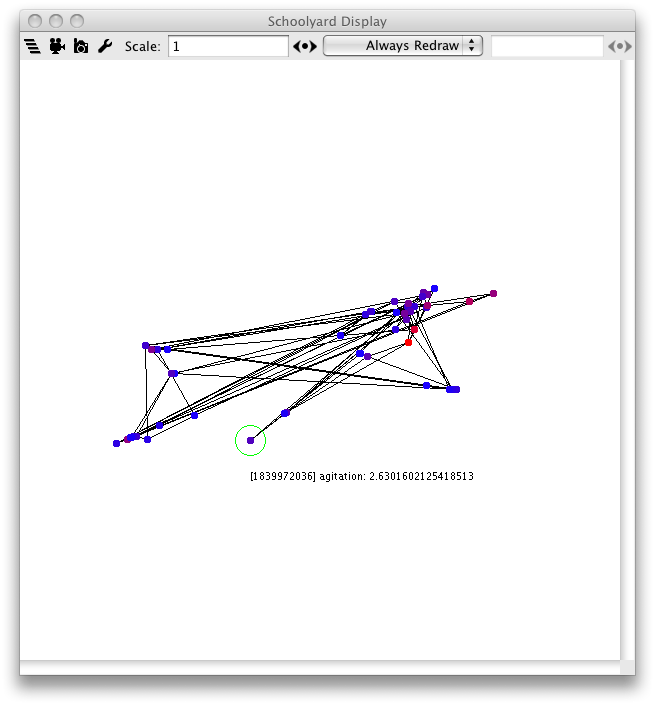
\includegraphics[width=3in]{Schoolyard4.png}\vspace{-2em}\end{wrapfigure}

As can be seen in the Display to the right, when you click (once) on a node, it is circled in green and given a useful label; any other nodes you happened to hit will also be selected.  If you click elsewhere, the original node is deselected.  And you can now drag objects and move them around the environment.  Try it!

Selection and dragging works for continuous environments and certain gridworld scenarios.  At present you can't select or drag edges.

Selection is presently somewhat primitive: you can't band-select (create a rectangle and select all the elements in it) nor hold down the shift key and select/deselect objects selectively.  And though you can select more than one object at a time, you can't present move more than one object at a time.  Perhaps in a later version.

\section{Add an Anonymous Agent}

Let's add an additional agent which, if used, initially sets the randomness to a high value and gradually decreases it.  The user can turn the agent off in the model inspector.  The point of this exercise is twofold.  First, it demonstrates the use of an {\bf anonymous class} to add a single agent to the schedule (a common practice).  Second, it introduces the notion of an {\bf explicit ordering} among agents scheduled at the exact same timestep.

MASON uses anonymous classes a lot, so if you're not familiar with them, they're worth explaining.  An anonymous class is simply a class that has no name at all.\footnote{Well, technically {\it all} Java classes have names.  But since you didn't state one, the compiler is free to make one up, which it will.  \file{javac} will probably name it \class{Foo\${\it number}}, for some arbitrary number, if the outer class in which it is declared is named \class{Foo}.} Instead, the anonymous class exists solely to be the subclass of some other class, or implement some interface,  then  create a single instance, and go away.

The pattern for anonymous classes is:

\begin{alltt}\small
new \textit{SuperclassOrInterface}()
    \{
    \textit{methods and instance variables go here}
    \}
\end{alltt}

This pattern is an {\it expression} which creates a single instance of a nameless class which subclasses from (or implements) \texttt{\textit{SuperclassOrInterface}}, and you can assign it to a variable or whatnot which is of the type \texttt{\textit{SuperclassOrInterface}}.  For example, we might create a subclass of \Class{javax.swing.JPanel} which overrides the method \method{paintComponent(...)}:

\begin{alltt}\small
JPanel myJPanel = new JPanel()
    \{
    public void paintComponent(Graphics g) \{ g.setColor(Color.black); g.drawLine(0,0,100,100); \}
    \};
\end{alltt}

Crucially, anonymous classes can access both the instance variables of the classes in which they are declared, and more interestingly, any {\bf final local variables} in the environment in which they were created.  For example, we could create a method which generates JPanels customized to your desired color:

\begin{alltt}\small
public JPanel makeJPanel(final Color color)
    \{
    return new JPanel()
        \{
        public void paintComponent(Graphics g) \{ g.setColor(color); g.drawLine(0,0,100,100); \}
        \};
    \}
\end{alltt}

This creates new JPanel subclasses on the fly with custom \method{paintComponent(...)} methods, produces single instances of them, and returns those instances.  Nifty.

Notice that \variable{color} had to be declared {\bf final}.  This isn't the case for outer instance variables used by anonymous classes, but it is the case for local variables and method parameters.\footnote{Why is this the case?  Beats me.  Any decent modern language contains {\bf closures}\,---\,which translate to {\it non}-final outer local variables usable by anonymous classes (or in many other languages, anonymous functions).  Closures are very useful, but require cleverness in compilation.  Sun's apparently not very clever.  The amazing thing is that you can hack the same thing with a work-around: instead of making a local variable \variable{final int foo = 4;}, you can make the variable \variable{final int[] foo = new int[] \{4\};}  Then you can modify \variable{foo}, from within the inner class, or more correctly, you can modify the value stored inside the array even if you can't change the array.  Why Sun didn't just bake this into the compiler, instead of requiring a hack work-around, is utterly beyond me.}

An anonymous class will save us the tedium of creating a new file for our class, and various casts or constructors.  So we're going with it.\footnote{Anonymous classes also make it possible to create an agent which is scheduled {\it twice} on the schedule, with different methods called each time, even though there's only {\it one} \method{step(...)} method.  If you have an agent with methods like this:\\

\noindent{\tt public class MyAgent\\
\indent\{\\
\indent public void doThis(SimState state) \{ ... \}\\
\indent public void doThat(SimState state) \{ ... \}\\
\indent\}\\
}

... you can just say:\\

\noindent{\tt final MyAgent agent = ...     // notice that the variable is declared final\\
schedule.scheduleRepeating(new Steppable() \{ public void step(SimState state) \{ agent.doThis(state); \}\});\\
schedule.scheduleRepeating(new Steppable() \{ public void step(SimState state) \{ agent.doThat(state); \}\});\\
}

... or whatever.}
We'll schedule the agent differently than the other agents: it'll occur at the same timestep as the others, but it will always be stepped {\it after} the other agents.  We do this by specifying an ordering of 1 for the agent.  The default ordering value for agents is 0.  When the schedule has extracted all the agents for a given timestep and is ready to step them, it first sorts them by their ordering (lower values first).  It then breaks ties with random shuffling. The method we'll use is \method{scheduleRepeating({\it time}, {\it ordering}, {\it Steppable})}.

So enough talking, here's the code.  See if you can make sense of it.  Note that for all the discussion above, our anonymous agent uses an instance variable of the outer class (\variable{tempering}) and so doesn't need to have it declared final.  We could have also used \method{isTempering()} instead of \variable{tempering}\,---\,anonymous classes have access to the methods of their outer instances.

{\footnotesize \begin{alltt}{\color{gray}import sim.engine.*;
import sim.util.*;
import sim.field.continuous.*;
import sim.field.network.*;

public class Students extends SimState
    \{
    public Continuous2D yard = new Continuous2D(1.0,100,100);}
    
    public double TEMPERING_CUT_DOWN = 0.99;
    public double TEMPERING_INITIAL_RANDOM_MULTIPLIER = 10.0;
    public boolean tempering = true;
    public boolean isTempering() \{ return tempering; \}
    public void setTempering(boolean val) \{ tempering = val; \}
	
    {\color{gray}public int numStudents = 50;

    double forceToSchoolMultiplier = 0.01;
    double randomMultiplier = 0.1;

    public int getNumStudents() \{ return numStudents; \}
    public void setNumStudents(int val) \{ if (val > 0) numStudents = val; \}

    public double getForceToSchoolMultiplier() \{ return forceToSchoolMultiplier; \}
    public void setForceToSchoolMultiplier(double val) \{ if (forceToSchoolMultiplier >= 0.0) forceToSchoolMultiplier = val; \}

    public double getRandomMultiplier() \{ return randomMultiplier; \}
    public void setRandomMultiplier(double val) \{ if (randomMultiplier >= 0.0) randomMultiplier = val; \}
    public Object domRandomMultiplier() \{ return new sim.util.Interval(0.0, 100.0); \}

    public double[] getAgitationDistribution()
        \{
        Bag students = buddies.getAllNodes();
        double[] distro = new double[students.numObjs];
        int len = students.size();
        for(int i = 0; i < len; i++)
            distro[i] = ((Student)(students.get(i))).getAgitation();
        return distro;
        \}

    public Network buddies = new Network(false);

    public Students(long seed)
        \{
        super(seed);
        \}

    public void start()
        \{
        super.start();}
        
        // add the tempering agent
        if (tempering)
            \{
            randomMultiplier = TEMPERING_INITIAL_RANDOM_MULTIPLIER;
            schedule.scheduleRepeating(schedule.EPOCH, 1, new Steppable() 
                 \{
                 public void step(SimState state) \{ if (tempering) randomMultiplier *= TEMPERING_CUT_DOWN; \} 
                 \});
            \}
		
        {\color{gray}// clear the yard
        yard.clear();

        // clear the buddies
        buddies.clear();
        
        // add some students to the yard
        for(int i = 0; i < numStudents; i++)
            \{
            Student student = new Student();
            yard.setObjectLocation(student, 
                new Double2D(yard.getWidth() * 0.5 + random.nextDouble() - 0.5,
                    yard.getHeight() * 0.5 + random.nextDouble() - 0.5));

            buddies.addNode(student);
            schedule.scheduleRepeating(student);
            \}
        
        // define like/dislike relationships
        Bag students = buddies.getAllNodes();
        for(int i = 0; i < students.size(); i++)
            \{
            Object student = students.get(i);
            
            // who does he like?
            Object studentB = null;
            do
                \{
                studentB = students.get(random.nextInt(students.numObjs));
                \} while (student == studentB);
            double buddiness = random.nextDouble();
            buddies.addEdge(student, studentB, new Double(buddiness));

            // who does he dislike?
            do
                \{
                studentB = students.get(random.nextInt(students.numObjs));
                \} while (student == studentB);
            buddiness = random.nextDouble();
            buddies.addEdge(student, studentB, new Double( -buddiness));
            \}
        \}
        
    public static void main(String[] args)
        \{
        doLoop(Students.class, args);
        System.exit(0);
        \}    
    \}}
\end{alltt}}

\paragraph{Compile and Run}

{\footnotesize \begin{alltt}
\textit{javac StudentsWithUI.java Students.java Student.java
java StudentsWithUI}
\end{alltt}}

Notice that now the agents start off jittery but calm down gradually.  That's the work of our tempering agent.  Also notice that you can turn off the effect in the \textit{Model} tab under the property \textit{Tempering}.  

\section{Checkpoint the Simulation}

One of MASON's hallmarks is its ability to do {\bf checkpointing}.  By this I mean the ability to save out the state of the simulation, mid-run, to a file on the disk.  The simulation can restart from this checkpoint even if it's on a different machine, or under visualization versus running on the command line, or even under a {\it different} visualization.  Let's see how that works.

\paragraph{Generate Some Checkpoints}

Run MASON in the following way:

{\footnotesize \begin{alltt}
\textit{java Students -docheckpoint 100000}

MASON Version 15.  For further options, try adding ' -help' at end.
Job: 0 Seed: 1293662957282
Starting Students
Steps: 25000 Time: 24999 Rate: 18,628.91207
Steps: 50000 Time: 49999 Rate: 25,562.37219
Steps: 75000 Time: 74999 Rate: 25,536.26149
Steps: 100000 Time: 99999 Rate: 25,510.20408
Checkpointing to file: 100000.0.Students.checkpoint
Steps: 125000 Time: 124999 Rate: 16,869.09582
Steps: 150000 Time: 149999 Rate: 19,888.62371
Steps: 175000 Time: 174999 Rate: 19,669.55153
Steps: 200000 Time: 199999 Rate: 19,888.62371
Checkpointing to file: 200000.0.Students.checkpoint
Steps: 225000 Time: 224999 Rate: 19,215.9877
Steps: 250000 Time: 249999 Rate: 19,700.55162

{\it ... etc. ...}
\end{alltt}}

Notice that MASON writes out a checkpoint every 100000 steps as requested.  What use are these?  There are a lot of uses.

For example, imagine that you've been running your simulation on a back-end supercomputer server for quite some time, and your job gets killed by the system administrator.  You can just go back to the most recent checkpoint and do this:

{\footnotesize \begin{alltt}
\textit{java Students -checkpoint 200000.0.Students.checkpoint -docheckpoint 100000}

MASON Version 15.  For further options, try adding ' -help' at end.
Loading from checkpoint 200000.0.Students.checkpoint
Recovered job: 0 Seed: 1293662957282
Steps: 225000 Time: 224999 Rate: 17,730.49645
Steps: 250000 Time: 249999 Rate: 24,154.58937
Steps: 275000 Time: 274999 Rate: 24,826.21648
Steps: 300000 Time: 299999 Rate: 25,100.40161
Checkpointing to file: 300000.0.Students.checkpoint
Steps: 325000 Time: 324999 Rate: 18,968.13354
Steps: 350000 Time: 349999 Rate: 19,685.03937

{\it ... etc. ...}
\end{alltt}}

MASON started up right where it left off as if nothing happened.  You can also load the checkpoint in the GUI:

\begin{itemize}
\item Execute {\tt java StudentsWithUI}
\item Select {\it Open...} from the {\it File} menu \raisebox{-0.1em}{
\includegraphics[scale=0.4]{FileMenu.png}}
\item Select the checkpoint.
\item The simulation loads the checkpoint and waits for you to unpause and continue it. 
\end{itemize}

You can also save out a checkpoint from the GUI:

\begin{itemize}
\item Select {\it Save As...} from the {\it File} menu \raisebox{-0.1em}{
\includegraphics[scale=0.4]{FileMenu.png}}
\item Save out the checkpoint.
\end{itemize}

This saved-out checkpoint is just like any other: you could start it up again from the command line on your back-end machine.  Or you could load it under a different GUI you've constructed.\footnote{Interested in seeing the transfer of a checkpoint between different GUI approaches?  Try the examples \Class{sim.app.heatbugs.HeatBugsWithUI} versus \Class{sim.app.heatbugs3d.HeatBugs3DWithUI}, both of which use the same exact model.}

\paragraph{A Note on Serialization}

MASON's checkpointing uses Java Serialization to do its magic, and Java Serialization is a fickle thing.  To work properly, every object in the model (agents on the schedule, objects stored in fields, etc.) must implement the \Class{java.io.Serializable} interface.  That's one of several reasons why you shouldn't put GUI objects on the Schedule: generally speaking Java's GUI widgets are not serializable.

One gotcha in Serialization is making sure that all inner classes and anonymous classes are Serializable, as well as their outer classes.  If your anonymous class is of type Steppable and thus an agent, for example, you're fine (Steppable is Serializable).  But make certain.

Another gotcha lies in the generation of so-called {\it serial version UID values}, essentially hashes of classes which Java uses to determine whether the class declaration in the serialized file is compatible with the classes is using.  Different Java implementations produce these hashes differently.  If you're using the same Java VM, compiler, and OS, you're fine.  But if you move class files from one machine to another (for example), there's no guarantee that the UID values will match.  This is particularly problematic for inner classes, anonymous classes, and outer classes of inner classes.

Much of this is because Java's approach to UIDs has proven historically misguided.  The solution is easy: rather than let Java generate the UID value, you declare it yourself.  I suggest declaring all UID values to \variable{1L} (a common practice) to bypass them entirely.  You should declare the following instance variable in all inner classes, all anonymous classes, all outer classes of inner classes, and (for good measure) all regular classes that you want to serialize, basically anything that's part of your model:

\java{%
private static final long serialVersionUID = 1L;
}

In our case, this instance variable should be added to the following classes:

\begin{itemize}
\item \class{Student}
\item \class{Students}
\item The anonymous class we declared as part of \class{Students} which decreased the randomness each timestep.
\end{itemize}

\section{Add a Description} 

\begin{figure}[t]\noindent\begin{center}%
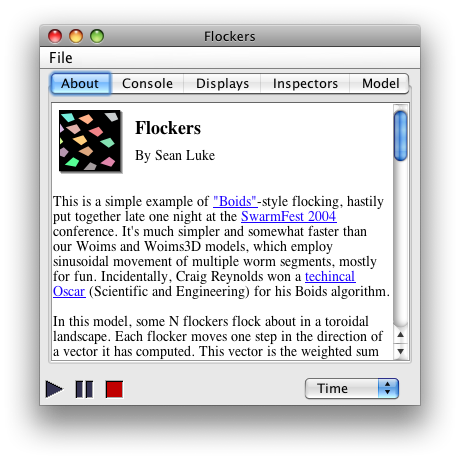
\includegraphics[height=2.1in]{FlockersConsole.png}%
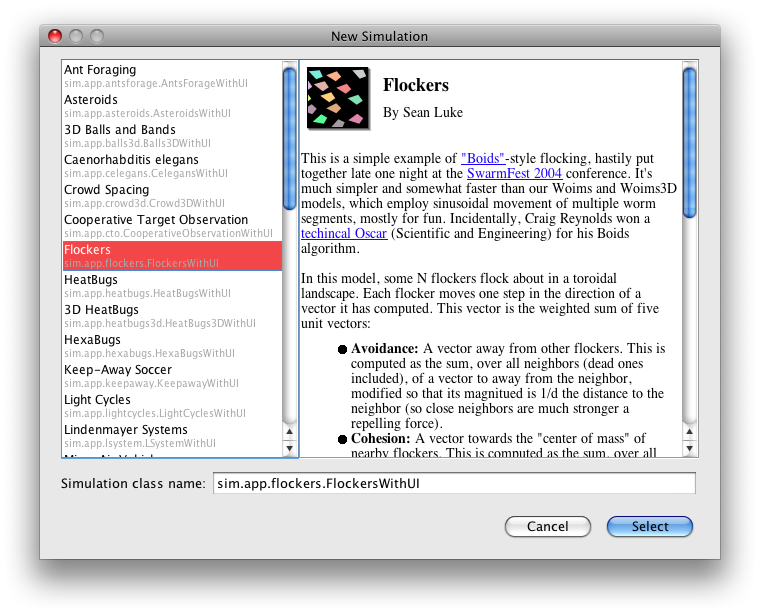
\includegraphics[height=2.8in]{NewSimulationPanel.png}%
\end{center}%
\caption{The Console and the Simulation-Chooser Window, both showing the HTML descriptive text of a simulation.}%
\label{ConsoleAndSimulationChooser}
\end{figure}

MASON has a simple built-in HTML viewer which lets you decorate your simulation with some descriptive text.  This text will appear in two places:

\begin{itemize}
\item Under the {\bf About Tab} \raisebox{-0.25em}{
\includegraphics[scale=0.4]{AboutButton.png}}
\item In the pop-up simulation-chooser window which appears when you choose {\it New Simulation...} from the {\bf File Menu} \raisebox{-0.1em}{
\includegraphics[scale=0.4]{FileMenu.png}}
\end{itemize}

\sidebar{Is there any way to go directly to the simulation-chooser window when I start MASON?}{Of course.  Run MASON like this:

{\footnotesize \begin{alltt}
\textit{java sim.display.Console}
\end{alltt}}

\noindent This is also how MASON is started if you use any of the scripts in the \file{mason/start} directory.

If you hit the ``Cancel'' button when firing MASON up this way, the program will simply quit.
}
These two situations are shown in Figure \ref{ConsoleAndSimulationChooser}.  MASON allows you to provide an HTML file, a String description (which may or may not be HTML), or a URL.

It's very easy to add an HTML file.  Simply create a file called \file{index.html} located right next to the class file of your GUIState subclass.  MASON will load the file and display it when your simulation is fired up.

For example, create the following file, named \file{index.html}, and save it right next to the file \file{StudentsWithUI.class}:

{\footnotesize \begin{alltt}<!DOCTYPE HTML PUBLIC "-//W3C//DTD HTML 3.2 Final//EN">
<html>
<head>
</head>
<body>

<table border=0 cellspacing=0 cellpadding=6>
<tr>
<td valign=top>
        <img src="icon.png">
<td valign=top>
        <h2>Student Cliques</h2>
        <b>Tutorial</b>
</table>

<p>
A fictional model of student clique formation on playgrounds.  Students form a social network of varying
degrees of mutual friendship or dislike.  Once let out of school, students try to move towards friends and
away from enemies.  Additional forces tug on students to keep them near near the schoolhouse (the center
of the yard), and to add some randomness.  Students change from red to blue as they become happier with
their situation.

</body>
</html>
\end{alltt}}

Notice that the DOCTYPE indicates HTML 3.2, an old and simple version of HTML with limited CSS support.  This is as far as Java's GUI facilities go.  You do not need to provide the DOCTYPE: but you do need to be aware that 3.2 is all MASON can display.

\begin{wrapfigure}{r}[0in]{1in}
\vspace{-1em}\hfill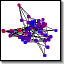
\includegraphics[width=0.5in]{SchoolyardIcon.png}\vspace{-0em}\end{wrapfigure}

The HTML file above requires an image (\file{icon.png}) to provide sort of the ``standard look'' of MASON's built-in demo applications.  The one I use is shown at right.


\begin{wrapfigure}{r}[0in]{3in}
\vspace{-5em}\hfill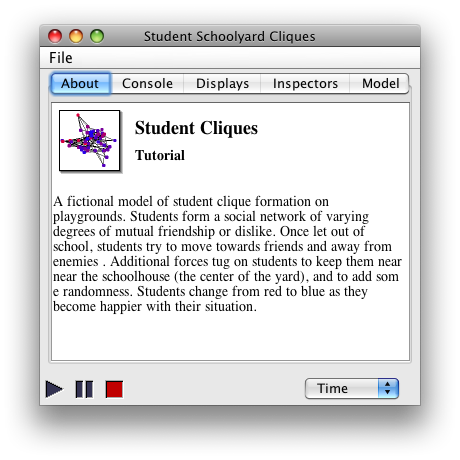
\includegraphics[width=2.8in]{Console2.png}\vspace{-7em}\end{wrapfigure}


\paragraph{Run the Simulation}
Now fire up the simulation again:

{\footnotesize \begin{alltt}
\textit{java StudentsWithUI}
\end{alltt}}

\noindent ... and the Console now looks like the Figure on the right.

Alternatively you can embed your own String, or a URL to an existing web page, directly in your GUIState subclass.  For example, if you didn't provide the \file{index.html} file above, you could add some simple text in the method \method{getInfo()}.  Specifically, add the following method to your \file{StudentsWithUI.java} file:

{\footnotesize \begin{alltt}
    public static Object getInfo()
        \{
        return "<h2>This is the tutorial</h2>" + 
            "<p>Pretty nifty!";
        \}
\end{alltt}}

With this static method in place, MASON will use its value rather than hunting for an \file{index.html} file.   But there's a gotcha.  

\sidebar{Wait, \method{getInfo()} is a static method.  You can't override static methods!}{Correct.  But MASON actually looks for the method using Java's reflection facility, so it's all good.  MASON does this so it can find and display the proper String or URL without having to instantiate a simulation.}
Java looks for image files referenced from an HTML file by looking relative to the HTML file itself.  Unfortunately if you override the \method{getInfo()} method, Java doesn't know where to look for images.  For example, the \file{icon.png} image would be broken.  So for the time being, you can't embed images or CSS files with relative URLs, or use relative URL links to other HTML files, if you override \method{getInfo()} to return a String.  In general, I suggest using the \file{index.html} file instead, unless you're just trying to display some simple text.

One last approach you can take is to return not a String but a URL.  For example, you could override \method{getInfo()} like this:


{\footnotesize \begin{alltt}
public static Object getInfo()
    \{
    try \{ return new java.net.URL("http://google.com/"); \} 
    catch (java.net.MalformedURLException e) \{ return "Oops"; \}
    \}
\end{alltt}}

\begin{wrapfigure}{r}[0in]{3in}
\vspace{-9em}\hfill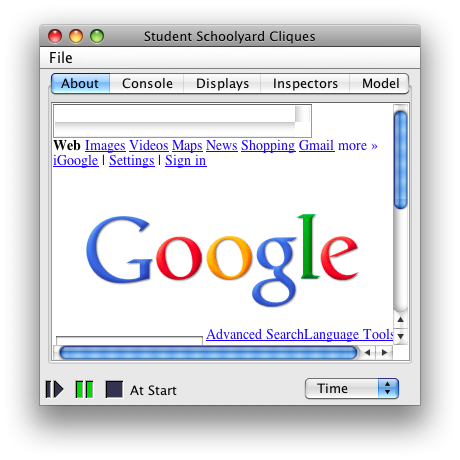
\includegraphics[width=2.8in]{Console3.png}\vspace{-5em}\end{wrapfigure}

When you do this, the Console window will look like it does at right.  Notice that the Google.com page is a bit discombobulated: it's assuming a more recent version of HTML than 3.2.  If you try it, you'll also find out that the search buttons don't work, though the links do.  I believe form submission in general isn't available in Java's basic HTML facilities (nor is JavaScript).




\bump

\section{Go 3D} 

MASON has as extensive a 3D model and visualization as it has a 2D one.  3D Visualization in MASON sits on top of Java3D, a scenegraph developed by Sun and widely available.  You don't need to know any Java3D at all to do visualization and model development in MASON, though just like AWT graphics and Java2D help in doing the 2D visualization, knowing a bit of Java3D will help to do advanced stuff in the 3D case.

Here we're going to add a simple 3D viewer to give you a taste of how to do visualization in 3D.  The 3D facility can visualize 2D fields, but obviously 3D fields are more fun.  So we'll start by creating a 3D field.  Let's make a 3D version of the playground, where the position of the student in the Z direction is the degree of agitation he presently has.

To do this, we'll provide the \file{Students.java} file with a \class{sim.field.continuous.Continuous3D} field.  Modify \file{Students.java} as follows:

{\footnotesize \begin{alltt}{\color{gray}import sim.engine.*;
import sim.util.*;
import sim.field.continuous.*;
import sim.field.network.*;

public class Students extends SimState
    \{
    public Continuous2D yard = new Continuous2D(1.0, 100, 100);}
    public Continuous3D agitatedYard = new Continuous3D(1.0, 100, 100, 100);
    
    {\color{gray}public double TEMPERING_CUT_DOWN = 0.99;
    public double TEMPERING_INITIAL_RANDOM_MULTIPLIER = 10.0;
    public boolean tempering = true;}
\end{alltt}}

... and on.  Continuous3D is basically the same as Continuous2D, except that it uses Double3D rather than Double2D.
The students will be placed in this field as well, but each timestep their locations will be simply updated by setting their X and Y positions to the same as in the Continuous2D, and setting their Z position to their agitation (plus a little scaling).  We add to \file{Students.java} the following method:


{\footnotesize \begin{alltt}
    public void load3DStudents()
        \{
        Bag students = buddies.getAllNodes();
        for(int i = 0; i < students.size(); i++)
            \{
            Student student = (Student)(students.get(i));
            Double2D loc = (Double2D)(yard.getObjectLocation(student));
            
            // we multiply by 5 in order to scale the agitation roughly with the student dispersion
            // in the other two dimensions
            agitatedYard.setObjectLocation(student, new Double3D(loc, student.getAgitation() * 5.0));
            \}
        \}
\end{alltt}}

We need to call this method two times.  First we need to call it each timestep.  Second, we need to call it at the end of the \method{start()} method so that the Continuous3D has students stored in it when it's first queried by the Network for their locations so the Network can draw edges in 3D.  We also need to clear the yard just like we cleared the 2D yard.

Modify the \method{start()} method in \file{Students.java} like this:

{\footnotesize \begin{alltt}{\color{gray}
    public void start()
        \{
        super.start();
        
        // add the tempering agent
        if (tempering)
            \{
            randomMultiplier = TEMPERING_INITIAL_RANDOM_MULTIPLIER;
            schedule.scheduleRepeating(schedule.EPOCH, 1, new Steppable() 
                 \{
                 public void step(SimState state) \{ if (tempering) randomMultiplier *= TEMPERING_CUT_DOWN; \} 
                 \});
            \}
                
        // clear the yard
        yard.clear();

        // clear the buddies
        buddies.clear();}
        
        agitatedYard.clear();
        
        {\color{gray}// add some students to the yard
        for(int i = 0; i < numStudents; i++)
            \{
            Student student = new Student();
            yard.setObjectLocation(student, 
                new Double2D(yard.getWidth() * 0.5 + random.nextDouble() - 0.5,
                    yard.getHeight() * 0.5 + random.nextDouble() - 0.5));

            buddies.addNode(student);
            schedule.scheduleRepeating(student);}
            Steppable steppable = new Steppable() 
                    \{
                    public void step(SimState state) \{ load3DStudents(); \}
                    \};
            schedule.scheduleRepeating(schedule.EPOCH, 2, steppable);
            {\color{gray}\}
        
        // define like/dislike relationships
        Bag students = buddies.getAllNodes();
        for(int i = 0; i < students.size(); i++)
            \{
            Object student = students.get(i);
            
            // who does he like?
            Object studentB = null;
            do
                \{
                studentB = students.get(random.nextInt(students.numObjs));
                \} while (student == studentB);
            double buddiness = random.nextDouble();
            buddies.addEdge(student, studentB, new Double(buddiness));

            // who does he dislike?
            do
                \{
                studentB = students.get(random.nextInt(students.numObjs));
                \} while (student == studentB);
            buddiness = random.nextDouble();
            buddies.addEdge(student, studentB, new Double( -buddiness));
            \}}
            
        load3DStudents();
        {\color{gray}\}}
\end{alltt}}

Notice that we scheduled an anonymous agent which simply calls \method{load3DStudents();}.  But this piece of code may have been confusing:

\java{%
            schedule.scheduleRepeating(schedule.EPOCH, 2, steppable);
}

Here we're scheduling the new anonymous agent with ordering 2, rather than the 0 the students use and the~1 used by the tempering anonymous agent.  This means that the agent will get stepped every timestep, but after all other agents are stepped.  That way we know the students have updated their agitation before we call the method (\method{load3DStudents()} which relocates them in the 3D field based on their agitation.

\paragraph{Compile and Run}  If you compile and run the command-line simulation at this point...

{\footnotesize \begin{alltt}
\textit{javac Students.java Student.java
java Students}
\end{alltt}}

\noindent ...you'll find that it should run fine.  But what does it look like?  Let's start in on the visualization.

\paragraph{Add Visualization in 3D} Java3D has a different collection of import needs than 2D Java.  Open the \file{StudentsWithUI.java} file and add the following imports:

{\footnotesize \begin{alltt}
import sim.display3d.*;
import sim.portrayal3d.continuous.*;
import sim.portrayal3d.network.*;
import sim.portrayal3d.simple.*;
import java.text.*;
import sim.field.network.*;
\end{alltt}}

Next we need to add a \class{sim.display3d.Display3D} and its JFrame, plus a \class{sim.portrayal3d.continuous.ContinuousPortrayal3D} and a \class{sim.portrayal3d.network.NetworkPortrayal3D}.  These classes are the 3D equivalents of Display2D, ContinuousPortrayal2D, and NetworkPortrayal2D, and you'll find they work similarly.  Add the following to \file{StudentsWithUI.java}:

{\footnotesize \begin{alltt}{\color{gray}
public class StudentsWithUI extends GUIState
    \{
    public Display2D display;
    public JFrame displayFrame;

    ContinuousPortrayal2D yardPortrayal = new ContinuousPortrayal2D();
    NetworkPortrayal2D buddiesPortrayal = new NetworkPortrayal2D();}
	
	
    public Display3D display3d;
    public JFrame displayFrame3d;
    ContinuousPortrayal3D agitatedYardPortrayal = new ContinuousPortrayal3D();
    NetworkPortrayal3D agitatedBuddiesPortrayal = new NetworkPortrayal3D();
\end{alltt}}

In the 2D case, we needed to set the field and the Simple Portrayal for the 2D yard and buddies field portrayals.  We'll do the same thing in the 3D case.  Our students will be represented by red unlit\footnote{A term of art in 3D graphics meaning ``visible even when there are no lights turned on''.} cones via \class{sim.portrayal3d.simple.ConePortrayal3D}.  We'll scale them to them twice their normal size (2.0).  Our buddies edges will be represented by gray cylinders via \class{sim.portrayal3d.simple.ConePortrayal3D}.  For grins, we'll label the edges with the edge weight by overriding the \method{getLabel(...)} method.  Because space is tight, we'll make the labels half their normal size.  The buddies field portrayal will use a SpatialNetwork3D, which works more or less identically to the SpatialNetwork2D used in the 2D case.

This will all be done in the \method{setupPortrayals()} method.  At the very end of this method we need to set up the 3D display.  In the 2D cases we had to reset the display and repaint it.  In the 3D case we instead do the following incantation:

\java{%
display3d.createSceneGraph();\\
display3d.reset();
}

The \method{createSceneGraph()} method instructs the 3D display to load all of its 3D objects and start displaying them.  It's the rough equivalent, in the MASON visualization parlance, of what \method{repaint()} was in the 2D case.

Modify the \method{setupPortrayals()} method in \file{StudentsWithUI.java} as follows:

{\footnotesize \begin{alltt}{\color{gray}
    public void setupPortrayals()
        \{
        Students students = (Students) state;
        
        // tell the portrayals what to portray and how to portray them
        yardPortrayal.setField( students.yard );
        yardPortrayal.setPortrayalForAll(
            new MovablePortrayal2D(
                new CircledPortrayal2D(
                    new LabelledPortrayal2D(
                        new OvalPortrayal2D()
                            \{
                            public void draw(Object object, Graphics2D graphics, DrawInfo2D info)
                                \{
                                Student student = (Student)object;

                                int agitationShade = (int) (student.getAgitation() * 255 / 10.0);
                                if (agitationShade > 255) agitationShade = 255;
                                paint = new Color(agitationShade, 0, 255 - agitationShade);
                                super.draw(object, graphics, info);
                                \}
                            \}, 
                        5.0, null, Color.black, true),
                    0, 5.0, Color.green, true)));
                                                

        
        buddiesPortrayal.setField( new SpatialNetwork2D( students.yard, students.buddies ) );
        buddiesPortrayal.setPortrayalForAll(new SimpleEdgePortrayal2D());

        // reschedule the displayer
        display.reset();
        display.setBackdrop(Color.white);

        // redraw the display
        display.repaint();}
        
        
        agitatedYardPortrayal.setField( students.agitatedYard );
        agitatedYardPortrayal.setPortrayalForAll(new ConePortrayal3D(Color.red, 2.0));

        agitatedBuddiesPortrayal.setField( new SpatialNetwork3D( students.agitatedYard, students.buddies ) );
        SimpleEdgePortrayal3D ep = new CylinderEdgePortrayal3D()
            \{
            DecimalFormat format = new DecimalFormat("#.##");
                
            public String getLabel(Edge edge)
                \{
                return "" + format.format(edge.getWeight());
                \}
            \};
            
        ep.setLabelScale(0.5);
        agitatedBuddiesPortrayal.setPortrayalForAll(ep);
        
        display3d.createSceneGraph(); 
        display3d.reset();
        \}
\end{alltt}}

Now we need to set up the Display3D in the \method{init()} method.  It's exactly like setting up the Display2D except we're optionally translating and scaling the scene that's going to be displayed.  The translation moves it so that the X and Y portions are centered at the origin (just as they're centered in the middle of the 2D screen) but the Z portion stays as it is.   We typically scale Java3D scenes by \(1.0 / W\) or \(2.0 / W\) where \(W\) is the maximum extent of the scene\,---\,perhaps the width of the field.  This sets them up to roughly fill a cube 1 or 2 units on a side, which looks good given the standard position of the 3D camera.

Also we'll make the Display3D window smaller for no good reason (you can change it).  Modify the \method{init()} method as follows:

{\footnotesize \begin{alltt}{\color{gray}
    public void init(Controller c)
        \{
        super.init(c);

        // make the displayer
        display = new Display2D(600,600,this);
        // turn off clipping
        display.setClipping(false);

        displayFrame = display.createFrame();
        displayFrame.setTitle("Schoolyard Display");
        c.registerFrame(displayFrame);   // register the frame so it appears in the "Display" list
        displayFrame.setVisible(true);
        display.attach( buddiesPortrayal, "Buddies" );
        display.attach( yardPortrayal, "Yard" );}

        display3d = new Display3D(300, 300,this);
        double width = 100;
        display3d.translate(-width / 2.0, -width / 2.0, 0);
        display3d.scale(2.0 / width);

        displayFrame3d = display3d.createFrame();
        displayFrame3d.setTitle("Schoolyard Display... NOW IN 3-D!");
        c.registerFrame(displayFrame3d);   // register the frame so it appears in the "Display" list
        displayFrame3d.setVisible(true);
        display3d.attach( agitatedBuddiesPortrayal, "Buddies ... IN 3-D!" );
        display3d.attach( agitatedYardPortrayal, "Yard ... IN 3-D!" );
        {\color{gray}\}}
\end{alltt}}
        
You might want to move the Display3D frame so it's not overlapping on top of the Display2D frame, but we'll not bother here.  All that remains is to shut down the Display3D just like we shut down the Display2D.  Modify the \method{quit()} method like this:

{\footnotesize \begin{alltt}{\color{gray}
    public void quit()
        \{
        super.quit();

        if (displayFrame!=null) displayFrame.dispose();
        displayFrame = null;
        display = null;}
		
        if (displayFrame3d!=null) displayFrame3d.dispose();
        displayFrame3d = null;
        display3d = null;
        {\color{gray}\}}
\end{alltt}}

And we're done!

\paragraph{Compile and Run}  If you compile and run the simulation...

{\footnotesize \begin{alltt}
\textit{javac StudentsWithUI.java Students.java Student.java
java StudentsWithUI}
\end{alltt}}

\begin{wrapfigure}{r}[0in]{3in}
\vspace{-14em}\hfill\includegraphics[width=2.8in]{Students3D.png}\vspace{-2em}\end{wrapfigure}

\noindent ...you should fine a new Display added to your simulation which looks like the figure to the right (I've enlarged the window a bit\,---\,try dragging in the bottom right corner to do that.).  You can {\bf rotate} the scene by dragging on it, {\bf translate} the scene by right-mouse-button-dragging or by dragging with the Command key pressed, and finally {\bf move the camera towards or away from the scene} by middle-mouse-button-dragging or by dragging with the Option/Alt key pressed.  You'll find that double-clicking on objects and edges in the 3D 
scene will bring up inspectors too.  And be sure to check out the options in the Options pane too: for example, auto-rotation, or adding axes.




\chapter{Basic Utility Classes}
\label{sim.util}

\begin{figure}[h]\vspace{-33em}\hspace{30em}\includegraphics[width=4in]{ants.pdf}\vspace{2em}\end{figure}


MASON has a large number of utility classes which can be used independently of the toolkit.  These classes fall in six packages:

\begin{itemize}
\item \package{ec.util}\quad The Mersenne Twister random number generator
\item \package{sim.util}\quad Basic utility classes
\item \package{sim.util.gui}\quad Graphical interface utility classes
\item \package{sim.util.media}\quad Utility classes for generating movies and pictures
\item \package{sim.util.media.chart}\quad Utility classes for generating charts
\item \package{sim.util.distribution}\quad Utility classes for sampling from distributions
\end{itemize} 

This chapter concentrates solely on \package{ec.util}, \package{sim.util}, and \package{sim.util.distribution}.  Many classes in the core simulation code rely on these packages (well the first two anyway), so it's important to cover them now.  The remaining packages will be covered in Chapter \ref{guiandmediautilities}.

\section{Random Number Generation}
\label{ec.util}
\label{ec.util.MersenneTwisterFast}
\label{sim.util.distribution}

The \package{ec.util} package contains a single class called \Class{ec.util.MersenneTwisterFast}.  This is an efficient implementation of the MT199937 Mersenne Twister algorithm by Makoto Matsumoto and Takuji Nishimura.  The Mersenne Twister is a well-regarded random number generator with an ultra-long period and high quality statistical properties.  It's now the standard generator for R, Maple, MATLAB, Python, Ruby, and several major implementations of Common Lisp (such as SBCL and CMUCL), and is part of the PHP library.  MASON uses Mersenne Twister as its only random number generator; it's possible to substitute another, but you'd need to subclass the MersenneTwisterFast class.

\paragraph{Why not use \class{java.util.Random?}}  Because \class{java.util.Random} is {\it highly non-random}.  It is unquestionably inappropriate for use in a high-quality simulator.  Never use it, nor should you ever call \method{Math.random()} (which also uses it).

\paragraph{Where did \package{ec.util} and \class{ec.util.MersenneTwisterFast} come from?}  This class and package came from ECJ, an evolutionary computation toolkit I developed in 1998.  There are actually two versions of Mersenne Twister: the class \class{ec.util.MersenneTwister} and the class \class{ec.util.MersenneTwisterFast}.  The former is a drop-in subclass replacement for \class{java.util.Random}, and is threadsafe.  The latter is not threadsafe, is {\it not} a subclass of \class{java.util.Random}, and has many methods (perhaps nowadays unnecessarily) heavily inlined, and as a result is significantly faster.  MersenneTwisterFast is the only class provided with and used by MASON.

\paragraph{Any gotchas?}  Yes.  The standard MT199937 seeding algorithm uses one of Donald Knuth's plain-jane linear congruential generators to fill the Mersenne Twister's arrays.  This means that for a short while the algorithm will initially be outputting a (very slightly) lower quality random number stream until it warms up.  After about 624 calls to the generator, it'll be warmed up sufficiently.   As a result, in \method{SimState.start()}, {\bf MASON primes the MT generator for you by calling \method{nextInt()} 1249 times.}

MersenneTwisterFast has identical methods to \class{java.util.Random}, plus one or two more for good measure. They should look familiar to you:

\begin{methods}{\class{ec.util.MersenneTwisterFast} Constructor}
\mthd{public MersenneTwisterFast(long seed)}  Seeds the random number generator.  Note that only the first 32 bits of the seed are used.
\mthd{public MersenneTwisterFast()}  Seeds the random number generator using the current time in milliseconds.
\mthd{public MersenneTwisterFast(int[] vals)}  Seeds the random number generator using the given array.  Only the first 624 integers in the array are used.  If the array is shorter than 624, then the integers are repeatedly used in a wrap-around fashion (not recommended).  The integers can be anything, but you should avoid too many zeros.  MASON does not call this method.
\end{methods}

\begin{methods}{\class{ec.util.MersenneTwisterFast}}
\mthd{public void setSeed(long seed)} Seeds the random number generator.  Note that only the first 32 bits of the seed are used.
\mthd{public void setSeed(int[] vals)} Seeds the random number generator using the given array.  Only the first 624 integers in the array are used.  If the array is shorter than 624, then the integers are repeatedly used in a wrap-around fashion (not recommended).  The integers can be anything, but you should avoid too many zeros.
\mthd{public double nextDouble()} Returns a random double drawn in the half-open interval from [0.0, 1.0).  That is, 0.0 may be drawn but 1.0 will never be drawn.
\mthd{public double nextDouble(boolean includeZero, boolean includeOne)} Returns a random double drawn in interval from 0.0 to 1.0, possibly including 0.0 or 1.0 or both, as specified in the arguments.
\mthd{public float nextFloat()} Returns a random float drawn in the half-open interval from [0.0f, 1.0f).  That is, 0.0f may be drawn but 1.0f will never be drawn.
\mthd{public float nextFloat(boolean includeZero, boolean includeOne)} Returns a random float drawn in interval from 0.0f to 1.0f, possibly including 0.0f or 1.0f or both, as specified in the arguments.
\mthd{public double nextGaussian()} Returns a random double drawn from the standard normal Gaussian distribution (that is, a Gaussian distribution with a mean of 0 and a standard deviation of 1).
\mthd{public long nextLong()} Returns a random long.
\mthd{public long nextLong(long n)} Returns a random long drawn from between 0 to \(n-1\) inclusive.
\mthd{public int nextInt()} Returns a random integer.
\mthd{public int nextInt(int n)} Returns a random integer drawn from between 0 to \(n-1\) inclusive.
\mthd{public short nextShort()} Returns a random short.
\mthd{public char nextChar()} Returns a random character.
\mthd{public byte nextByte()} Returns a random byte.
\mthd{public void nextBytes(byte[] bytes)} Fills the given array with random bytes.
\mthd{public boolean nextBoolean()} Returns a random boolean.
\mthd{public boolean nextBoolean(float probability)} Returns a random boolean which is true with the given probability, else false.  Note that you must carefully pass in a {\it float} here, else it'll use the {\it double} version below (which is twice as slow).
\mthd{public boolean nextBoolean(double probability)} Returns a random boolean which is true with the given probability, else false.
\mthd{public Object clone()}  Clones the generator.
\mthd{public boolean stateEquals(Object o)}  Returns true if the given Object is a MersenneTwisterFast and if its internal state is identical to this one.
\mthd{public void writeState(DataOutputStream stream)}  Writes the state to a stream.
\mthd{public void readState(DataInputStream stream)}  Reads the state from a stream as written by \method{writeState(...)}.
\mthd{public static void main(String[] args)} Performs a test of the code.
\end{methods}

\subsection{Distributions with COLT}
The MersenneTwisterFast class, like \class{java.util.Random}, provides random numbers from only two floating-point distributions: uniform and Gaussian.  What if you need numbers drawn from other distributions?  MASON provides a variety of distributions in the \Package{sim.util.distribution} package.  This package is a modified version of the distributions from the COLT/JET library.\footnote{http:/\!/acs.lbl.gov/software/colt/}  The modifications remove certain misfeatures of the library which make it difficult to serialize, unify a few utility classes, and most importantly, replace COLT's random number generator data types with Mersenne Twister.  You can just plug in your model's MersenneTwisterFast random number generator and pop out random numbers under various distributions.

Because it's separate from the MASON core proper (and a bit new), I don't describe this package in detail, but it should be fairly straightforward.  {\bf Warning:} the port of these classes from COLT to MASON is new and has not been tested much.

There are two kinds of distributions: (1) distributions which require their own instances and (2) distributions which just require function calls.  The first group each have their own classes, and you must create instances of them.  They include:

\begin{itemize}
\item Beta\hspace{\fill} \Class{sim.util.distribution.Beta}
\item Binomial\hspace{\fill} \Class{sim.util.distribution.Binomial}
\item Breit-Wigner (Lorentz)\hspace{\fill} \Class{sim.util.distribution.BreitWigner}
\item Mean-Square Breit-Wigner\hspace{\fill} \Class{sim.util.distribution.BreitWignerMeanSquare}
\item Chi-Square\hspace{\fill} \Class{sim.util.distribution.ChiSquare}
\item Empirical\hspace{\fill} \Class{sim.util.distribution.Empirical}
\item Discrete Emperical\hspace{\fill} \Class{sim.util.distribution.EmpiricalWalker}
\item Exponential\hspace{\fill} \Class{sim.util.distribution.Exponential}
\item Exponential Power\hspace{\fill} \Class{sim.util.distribution.ExponentialPower}
\item Gamma\hspace{\fill} \Class{sim.util.distribution.Gamma}
\item Hyperbolic\hspace{\fill} \Class{sim.util.distribution.Hyperbolic}
\item Hyper-Geometric\hspace{\fill} \Class{sim.util.distribution.HyperGeometric}
\item Logarithmic\hspace{\fill} \Class{sim.util.distribution.Logarithmic}
\item Negative Binomial\hspace{\fill} \Class{sim.util.distribution.NegativeBinomial}
\item Normal (Gaussian)\,---\,not very useful as it's built into Mersenne Twister\hspace{\fill} \Class{sim.util.distribution.Normal}
\item Poisson (two kinds)\hspace{\fill} \Class{sim.util.distribution.Poisson} and \Class{sim.util.distribution.PoissonSlow} 
\item Student's T\hspace{\fill} \Class{sim.util.distribution.StudentT}
\item Uniform\,---\,again, not very useful as it's built into Mersenne Twister\hspace{\fill} \Class{sim.util.distribution.Uniform}
\item Von Mises\hspace{\fill} \Class{sim.util.distribution.VonMises}
\item Zeta\hspace{\fill} \Class{sim.util.distribution.Zeta}
\end{itemize}

The second group are just function calls from the \Class{sim.util.distribution.Distributions} class:

\begin{itemize}
\item Burr (various kinds)
\item Cauchy
\item Erlang
\item Geometric
\item Lambda
\item Laplace
\item Logistic
\item Power-Law
\item Triangular
\item Weibull
\item Zipf
\end{itemize}

\subsection{Distributions with Apache Commons Math}

An alternative is to use Apache Commons Math.\footnote{http://commons.apache.org/proper/commons-math/} Apache Commons has its own special interface for random number generators called \class{org.apache.commons.math3.random.RandomGenerator}.  To use its distributions, we must create a wrapper around MersenneTwisterFast which allows us to implement that interface.  It's easy:

\begin{verbatim}
public class MTFApache implements org.apache.commons.math3.random.RandomGenerator {
    ec.util.MersenneTwisterFast random;

    public MTFApache(ec.util.MersenneTwisterFast random) { this.random = random; }
    
    public boolean nextBoolean() { return random.nextBoolean(); }
    public void nextBytes(byte[] bytes) { random.nextBytes(bytes); }
    public double nextDouble() { return random.nextDouble(); }
    public float nextFloat() { return random.nextFloat(); }
    public double nextGaussian() { return random.nextGaussian(); }
    public int nextInt() { return random.nextInt(); }
    public int nextInt(int n) { return random.nextInt(n); }
    public long nextLong() { return random.nextLong(); }
    public void setSeed(int seed) { random.setSeed(seed); }
    public void setSeed(int[] array) { random.setSeed(array); }
    public void setSeed(long seed) { random.setSeed(seed); }
    }
\end{verbatim}

Armed with this class, we can now easily access distributions.  For example, we can say:

\begin{verbatim}
import org.apache.commons.math3.distribution.*;

LogNormalDistribution dist = new LogNormalDistribution(new MTFApache(state.random), 1.0, 1.0);  
System.err.println("Random LogNormal number: " + dist.sample());
\end{verbatim}

Note that Apache Commons Math distributions have alternative constructors which don't require that you pass in a random number generator\,---\,they build one internally.  This is a {\it very bad idea}, and whoever came up with this should be smacked.  {\bf Always pass in MersenneTwisterFast in a wrapper as the random number generator for your Apache Commons Math distribution when using MASON.}

\section{Coordinate Wrapper Classes}

MASON has a large number of consistent wrapper classes for 2D and 3D coordinates.  Java also has classes for 2D and 3D coordinates: for example, the \class{java.awt.Point} class wraps two integers (x and y), and the \class{java.awt.Point2D.Double} class wraps two doubles.  However Java's classes have severe deficiencies.  The most serious problem with them is that they are broken when used as keys in hash tables.  Sun in its infinite wisdom made a serious error in how it handles hashcode generation and equality testing in these classes, and so if you use them in hash tables, you will regret it.\footnote{Specifically: the classes hash by value rather than by pointer, yet they can have their values changed.  So if you hash an object keyed with a Point2D.Double, then change the values of the Point2D.Double, the object is lost in the hash table.}

To fix this, MASON has its own coordinate classes, in two forms, {\bf immutable} and {\bf mutable}.  Immutable instances may not have their values changed once set during instantiation.  The immutable classes work well as keys in hash tables.  Mutable instances can have their values changed freely.  MASON's mutable classes have the same problem as Sun's classes, but they are at least consistent, code-wise, with the immutable classes.  The mutable classes also have many more mathematical operations available.

The classes are:

\begin{itemize}
\item \Class{sim.util.Int2D} and \Class{sim.util.MutableInt2D}
\item \Class{sim.util.Double2D} and \Class{sim.util.MutableDouble2D}
\item \Class{sim.util.Int3D} and \Class{sim.util.MutableInt3D}
\item \Class{sim.util.Double3D} and \Class{sim.util.MutableDouble3D}
\end{itemize}

\sidebar{Why aren't these classes subclasses of one another?}{Interesting you asked that.  Let's ignore the incompatibility issues with final versus non-final instance variables.  Imagine if Int2D was as subclass of MutableInt2D.  Then Int2D would have to have various \method{set...()} methods because MutableInt2D had them, and it'd have to throw an exception on calling them, which would be ugly indeed.  Now imagine if MutableInt2D instead subclassed from Int2D.  Unfortunately then you couldn't make guarantees such as Int2D being safe for hashtables, because a subclass of it (MutableInt2D) wouldn't be.  It'd be plausible to have them subclass from a common class, but that runs the risk of the superclass again being misused as safe in hashtables.  So MASON keeps 'em separate.}
Though the classes have a zillion utility methods, in fact they are {\bf very simple wrappers over just two or three variables.}  Each of these classes has the following variables, which you can read and write directly (or at least read: in the immutable classes they're final):

\java{%
\hbox{int \textit{(or double)} x;}\\
\hbox{int \textit{(or double)} y;}\\
\hbox{int \textit{(or double)} z;  // in the 3D classes}
}

You should access these variables with abandon: they're designed for it.    Additionally the classes have many accessor methods.  We will show methods of the 2D versions of the classes below: the 3D classes are nearly identical (minus a few inappropriate methods here and there).  First up is Int2D:

\begin{methods}{\class{sim.util.Int2D} Constructor}
\mthd{public Int2D()}  Creates an Int2D with x=0 and y=0.
\mthd{public Int2D(int x, int y)}  Creates an Int2D with the given x and y values.
\mthd{public Int2D(java.awt.Point p)}  Creates an Int2D with x and y values of the given Point.
\mthd{public Int2D(MutableInt2D p)}  Creates an Int2D with x and y values of the given MutableInt2D.
\end{methods}

\begin{methods}{\class{sim.util.Int2D}}
\mthd{public int getX()} Returns the x value.
\mthd{public int getY()} Returns the y value.
\mthd{public java.awt.geom.Point2D.Double toPoint2D()} Builds a Point2D.Double with the current x and y values.
\mthd{public java.awt.Point toPoint()} Builds a Point with the current x and y values.
\mthd{public String toString()} Returns a String version of the Int2D.
\mthd{public String toCoordinates()} Returns a String version of the x and y values as coordinates in the form \((x, y)\).
\mthd{public int hashCode()} Builds a hash code from the Int2D.
\mthd{public boolean equals(Object obj)} Returns true if the Int2D is equal to the other object in value.  Int2D can be compared against other Int2D, MutableIn2D, Double2D, and MutableDouble2D objects.
\mthd{public double distance(double x, double y)} Returns the distance from the Int2D to the given coordinates.
\mthd{public double distance(Int2D p)} Returns the distance from the Int2D to the given coordinates.
\mthd{public double distance(MutableInt2D p)} Returns the distance from the Int2D to the given coordinates.
\mthd{public double distance(Double2D p)} Returns the distance from the Int2D to the given coordinates.
\mthd{public double distance(MutableDouble2D p)} Returns the distance from the Int2D to the given coordinates.
\mthd{public double distance(java.awt.geom.Point2D p)} Returns the distance from the Int2D to the given coordinates.
\mthd{public double distanceSq(double x, double y)} Returns the squared distance from the Int2D to the given coordinates.  This is faster than computing the distance (it doesn't require a square root).
\mthd{public double distanceSq(Int2D p)} Returns the squared distance from the Int2D to the given coordinates.  This is faster than computing the distance (it doesn't require a square root).
\mthd{public double distanceSq(MutableInt2D p)} Returns the squared distance from the Int2D to the given coordinates.  This is faster than computing the distance (it doesn't require a square root).
\mthd{public double distanceSq(Double2D p)} Returns the squared distance from the Int2D to the given coordinates.  This is faster than computing the distance (it doesn't require a square root).
\mthd{public double distanceSq(MutableDouble2D p)} Returns the squared distance from the Int2D to the given coordinates.  This is faster than computing the distance (it doesn't require a square root).
\mthd{public double distanceSq(java.awt.geom.Point2D p)} Returns the squared distance from the Int2D to the given coordinates.  This is faster than computing the distance (it doesn't require a square root).
\mthd{public long manhattanDistance(int x, int y)} Returns the manhattan distance from the Int2D to the given coordinates.
\mthd{public long manhattanDistance(Int2D p)} Returns the manhattan distance from the Int2D to the given coordinates.
\mthd{public long manhattanDistance(MutableInt2D p)} Returns the manhattan distance from the Int2D to the given coordinates.
\end{methods}

The distance between two points  \(\langle x_1, y_1\rangle\) and \(\langle x_2, y_2\rangle\) is defined as \(\sqrt{(x_1 - x_2)^2 + (y_1 - y_2)^2}\).  The squared distance is defined as \((x_1 - x_2)^2 + (y_1 - y_2)^2\).   The manhattan distance is defined as \(| x_1 - x_2|+ |y_1 - y_2|\).

MutableInt2D has all these methods and constructors, plus a few more:

\begin{methods}{Additional \Class{sim.util.MutableInt2D} Constructor}
\mthd{public MutableInt2D(Int2D)}  Creates a MutableInt2D with x and y values of the given Int2D.
\end{methods}

\begin{methods}{Additional \Class{sim.util.MutableInt2D}}
\mthd{public void setX(int val)} Sets the x value.
\mthd{public void setY(int val)} Sets the y value.
\mthd{public void setTo(int x, int y)} Sets the x and  y values.
\mthd{public void setTo(java.awt.Point p)} Sets the x and  y values to the given Point.
\mthd{public void setTo(Int2D p)} Sets the x and  y values to the given Int2D.
\mthd{public void setTo(MutableInt2D p)} Sets the x and  y values to the given MutableInt2D.
\mthd{public Object clone()} Returns a clone of the MutableInt2D.
\end{methods}

Double2D is similar to Int2D, though you'll find a few more constructors and useful mathematics functions:

\begin{methods}{\class{sim.util.Double2D} Constructor}
\mthd{public Double2D()}  Creates a Double2D with x=0 and y=0.
\mthd{public Double2D(double x, double y)}  Creates a Double2D with the given x and y values.
\mthd{public Double2D(java.awt.Point p)}  Creates a Double2D with x and y values of the given Point.
\mthd{public Double2D(java.awt.geom.Point2D.Double p)}  Creates a Double2D with x and y values of the given Point2D.Double.
\mthd{public Double2D(java.awt.geom.Point2D.Float p)}  Creates a Double2D with x and y values of the given Point2D.Float.
\mthd{public Double2D(MutableDouble2D p)}  Creates a Double2D with x and y values of the given MutableDouble2D.
\mthd{public Double2D(Int2D p)}  Creates a Double2D with x and y values of the given Int2D.
\mthd{public Double2D(MutableInt2D p)}  Creates a Double2D with x and y values of the given MutableInt2D.
\end{methods}

\begin{methods}{\class{sim.util.Double2D}}
\mthd{public double getX()} Returns the x value.
\mthd{public double getY()} Returns the y value.
\mthd{public java.awt.geom.Point2D.Double toPoint2D()} Builds a Point2D.Double with the current x and y values.
\mthd{public String toString()} Returns a String version of the Double2D.
\mthd{public String toCoordinates()} Returns a String version of the x and y values as coordinates in the form \((x, y)\).
\mthd{public int hashCode()} Builds a hash code from the Double2D.
\mthd{public boolean equals(Object obj)} Returns true if the Double2D is equal to the other object in value.  Double2D can be compared against Int2D, MutableIn2D, Double2D, and MutableDouble2D objects.
\mthd{public double distance(double x, double y)} Returns the distance from the Double2D to the given coordinates.
\mthd{public double distance(Int2D p)} Returns the distance from the Double2D to the given coordinates.
\mthd{public double distance(MutableInt2D p)} Returns the distance from the Double2D to the given coordinates.
\mthd{public double distance(Double2D p)} Returns the distance from the Double2D to the given coordinates.
\mthd{public double distance(MutableDouble2D p)} Returns the distance from the Double2D to the given coordinates.
\mthd{public double distance(java.awt.geom.Point2D p)} Returns the distance from the Double2D to the given coordinates.
\mthd{public double distanceSq(double x, double y)} Returns the squared distance from the Double2D to the given coordinates.  This is faster than computing the distance (it doesn't require a square root).
\mthd{public double distanceSq(Int2D p)} Returns the squared distance from the Double2D to the given coordinates.  This is faster than computing the distance (it doesn't require a square root).
\mthd{public double distanceSq(MutableInt2D p)} Returns the squared distance from the Double2D to the given coordinates.  This is faster than computing the distance (it doesn't require a square root).
\mthd{public double distanceSq(Double2D p)} Returns the squared distance from the Double2D to the given coordinates.  This is faster than computing the distance (it doesn't require a square root).
\mthd{public double distanceSq(MutableDouble2D p)} Returns the squared distance from the Double2D to the given coordinates.  This is faster than computing the distance (it doesn't require a square root).
\mthd{public double distanceSq(java.awt.geom.Point2D p)} Returns the squared distance from the Double2D to the given coordinates.  This is faster than computing the distance (it doesn't require a square root).
\mthd{public double manhattanDistance(double x, double y)} Returns the manhattan distance from the Double2D to the given coordinates.
\mthd{public double manhattanDistance(Double2D p)} Returns the manhattan distance from the Double2D to the given coordinates.
\mthd{public double manhattanDistance(MutableDouble2D p)} Returns the manhattan distance from the Double2D to the given coordinates.
\mthd{public double manhattanDistance(Int2D p)} Returns the manhattan distance from the Double2D to the given coordinates.
\mthd{public double manhattanDistance(MutableInt2D p)} Returns the manhattan distance from the Double2D to the given coordinates.
\mthd{public double manhattanDistance(java.awt.geom.Point2D p)} Returns the manhattan distance from the Double2D to the given coordinates.
\mthd{public double angle()} Returns the angle of the Double2D.
\mthd{public double length()} Returns the length of the Double2D.
\mthd{public double lengthSq()} Returns the squared length of the Double2D.  This is less expensive than calling \method{length()}, as it doesn't involve a square root.
\mthd{public double dot(Double2D other)} Takes the dot product of this and the other Double2D.
\mthd{public double perpDot(Double2D other)} Takes the ``perp dot product'' (the 2D equivalent of the cross product) of this and the other Double2D.
\mthd{public Double2D negate()} Returns the negation of this Double2D.
\mthd{public Double2D add(Double2D other)} Adds the other Double2D and returns a new Double2D holding the result.
\mthd{public Double2D subtract(Double2D other)} Subtracts the other Double2D and returns a new Double2D holding the result.
\mthd{public Double2D multiply(double scalar)} Multiplies the Double2D against the scalar and returns a new Double2D holding the result.
\mthd{public Double2D resize(double length)} Scales the Double2D to be the given length and returns a new Double2D holding the result.
\mthd{public Double2D normalize()} Normalizes the Double2D and returns a new Double2D holding the result.  If the Double2D is zero in length, an error is thrown.
\mthd{public Double2D rotate(double theta)} Rotates the Double2D by the given radians and returns a new Double2D holding the result.
\end{methods}

\paragraph{Example Usage}

Double2D is designed so that math operations produce new Double2D instances at each step.  For example, let's say you wanted to cause an agent \(\vec{a}\) to move away from enemies.  If an enemy \(e^{(i)}\) is close, it exerts a much higher force on the agent than if an enemy is far away.  We could have the agent add up all the forces, then move in a constant speed in the opposite direction.  Something along the lines of:

\[
	\vec{a} = \vec{a} + \delta \times \text{normalize}\left(\sum_i \frac{-1}{|\vec{e^{(i)}}|} \vec{e^{(i)}}\right)
\] 

We'd do it like this:

\java{%
double delta = ... \\
Double2D agent = ... \\
Double2D[] enemies = ... \\
Double2D force = new Double2D();  // <0,0> \\
for(int i = 0; i < enemies.length; i++)\\
\rule{4em}{0pt} force = force.add(enemies[i].multiply(-1.0 / enemies[i].length()));\\
agent~=~agent.add(force.normalize().multiply(delta));~//~alternatively~force.resize(delta)
}

Notice the chaining of operations in \code{force.normalize().multiply(delta)}.   Keep in mind that at every stage in these operations new Double2Ds are getting allocated, so this isn't amazingly efficient. If you're doing a lot of vector manipulation, you may instead wish to use a {\it mutable} version instead, which allows you to change certain vectors in-place:

\paragraph{Mutable Vectors}  The MutableDouble2D contains similar methods except for the \method{add()}, \method{subtract()}, \method{multiply()}, \method{resize()}, \method{normalize()}, and \method{rotate()} methods.  Instead MutableDouble2D methods tend to modify the MutableDouble2D itself instead of returning a brand new one (that's the point of MutableDouble2D after all).  Here are some of the different methods and constructors:

\begin{methods}{Additional \Class{sim.util.MutableDouble2D} Constructor}
\mthd{public MutableDouble2D(Double2D)}  Creates a MutableDouble2D with x and y values of the given Double2D.
\end{methods}


\begin{methods}{Additional \Class{sim.util.MutableDouble2D}}
\mthd{public void setX(double val)} Sets the x value.
\mthd{public void setY(double val)} Sets the y value.
\mthd{public void setTo(double x, double y)} Sets the x and  y values.
\mthd{public void setTo(java.awt.Point p)} Sets the x and  y values to the given Point.
\mthd{public void setTo(Int2D p)} Sets the x and  y values to the given Int2D.
\mthd{public void setTo(MutableInt2D p)} Sets the x and  y values to the given MutableInt2D.
\mthd{public void setTo(Double2D p)} Sets the x and  y values to the given Double2D.
\mthd{public void setTo(MutableDouble2D p)} Sets the x and  y values to the given MutableDouble2D.
\mthd{public Object clone()} Returns a clone of the MutableDouble2D.
\mthd{public MutableDouble2D addIn(double x, double y)} Modifies the MutableDouble2D to reflect adding in the other values.  Returns the modified MutableDouble2D.
\mthd{public MutableDouble2D addIn(Double2D other)} Modifies the MutableDouble2D to reflect adding in the other values.  Returns the modified MutableDouble2D.
\mthd{public MutableDouble2D addIn(MutableDouble2D other)} Modifies the MutableDouble2D to reflect adding in the other values.  Returns the modified MutableDouble2D.
\mthd{public MutableDouble2D add(MutableDouble2D other1, MutableDouble2D other2)} Adds other1 and other2, setting the Mutable2D to their sum and returning it.
\mthd{public MutableDouble2D add(Double2D other1, MutableDouble2D other2)} Adds other1 and other2, setting the Mutable2D to their sum and returning it.
\mthd{public MutableDouble2D add(MutableDouble2D other1, Double2D other2)} Adds other1 and other2, setting the Mutable2D to their sum and returning it.
\mthd{public MutableDouble2D subtractIn(Double2D other)} Modifies the MutableDouble2D to reflect subtracting the other values from it.  Returns the modified MutableDouble2D.
\mthd{public MutableDouble2D subtractIn(MutableDouble2D other)} Modifies the MutableDouble2D to reflect subtracting the other values from it.  Returns the modified MutableDouble2D.
\mthd{public MutableDouble2D subtract(MutableDouble2D other1, MutableDouble2D other2)} Subtracts other2 from other1 setting the Mutable2D to their difference and returning it.
\mthd{public MutableDouble2D subtract(Double2D other1, MutableDouble2D other2)} Subtracts other2 from other1 setting the Mutable2D to their difference and returning it.
\mthd{public MutableDouble2D subtract(MutableDouble2D other1, Double2D other2)} Subtracts other2 from other1 setting the Mutable2D to their difference and returning it.
\mthd{public MutableDouble2D multiplyIn(double scalar)} Modifies the MutableDouble2D to reflect multiplying it by the scalar.  Returns the modified MutableDouble2D.
\mthd{public MutableDouble2D multiply(MutableDouble2D other, double scalar)} Multiplies the other MutableDouble2D by the given scalar, setting this MutableDouble2D to the result.  Returns the modified MutableDouble2D.
\mthd{public MutableDouble2D multiply(Double2D other, double scalar)} Multiplies the Double2D by the given scalar, setting this MutableDouble2D to the result.  Returns the modified MutableDouble2D.
\mthd{public MutableDouble2D resize(double length)} Scales the MutableDouble2D to be the given length, modifying it, and returns it.
\mthd{public MutableDouble2D normalize()} Normalizes the MutableDouble2D , modifying it, and returns it.  If the MutableDouble2D is zero in length, an error is thrown.
\mthd{public MutableDouble2D rotate(double theta)} Rotates the MutableDouble2D by the given radians, modifying it, and returns it.
\mthd{public MutableDouble2D negate()} Negates the MutableDouble2D, modifying it, and returns it.
\mthd{public MutableDouble2D setToMinus(MutableDouble2D other)} Sets the MutableDouble2D to the negation of the other, and returns it.
\mthd{public MutableDouble2D zero()} Sets the MutableDouble2D to \(\langle 0,0\rangle\) and returns it.
\mthd{public MutableDouble2D dup()} Clones the MutableDouble2D.
\end{methods}

Whew!  As you can see, the general philosophy in the immutable classes is to create new immutable instances as a result of mathematical operations; whereas the mutable classes tend to modify themselves to reflect the results.

The 3D versions of these are very similar to the 2D, minus certain math operations (like perpDot or rotate) which make no sense in 3D.


\paragraph{Example Usage}  Returning to our previous example:

\[
	\vec{a} = \vec{a} + \delta \times \text{normalize}\left(\sum_i \frac{-1}{|\vec{e^{(i)}}|} \vec{e^{(i)}}\right)
\] 

Using MutableDouble2D we could do it a bit more efficiently like this:

\java{%
double delta = ... \\
Double2D agent = ... \\
Double2D[] enemies = ... \\
MutableDouble2D force = new MutableDouble2D();  // <0,0> \\
MutableDouble2D temp = new MutableDouble2D(); // <0,0> \\
for(int i = 0; i < enemies.length; i++)\\
\rule{4em}{0pt} force.addIn(temp.multiply(enemies[i], -1.0 / enemies[i].length()));\\
agent~=~agent.add(force.normalize().multiply(delta));~//~alternatively~force.resize(delta)
}

Here instead of creating new Double2Ds for each math step, we store the results in a temporary variable, and ultimately modify the \variable{force} variable.  At the end we dump the results into a Double2D again (Double2D is used for hashing in Continuous Fields (see Section \ref{sim.field.continuous}) and Mutable2D is not).

With modern garbage collection methods, allocating lots of Double2Ds is less of a concern, but it's still more than worthwhile to use MutableDouble2D in many situations. 

\section{Collections}
\label{sim.util.Indexed}

MASON has four collections classes special to it:

\begin{itemize}
\item \Class{sim.util.Bag} is an extensible array, quite similar to \class{java.util.ArrayList}.
 \item \Class{sim.util.IntBag} is like a Bag, but it holds ints rather than Objects.
 \item \Class{sim.util.DoubleBag} is like a Bag, but it holds doubles rather than Objects.
 \item \Class{sim.util.Heap} is a binary heap, similar to \class{java.util.PriorityQueue}.  Heap is discussed later in Section \ref{sim.util.Heap}.
 \end{itemize}
 
 \paragraph{Why create a new ArrayList?}  \Class{sim.util.Bag} was created because at the time (2004) most ArrayList operations were quite slow.  For years ArrayList's \method{get()}, \method{set()}, and \method{add()} operations were not inlinable!  In fact now they're inlinable only because of advances in Hotspot technology and not because of simple bug-fixes that could have been made in the class years ago (the bugs are still there).  
 
Bag is an extensible array like ArrayList but with four major differences:

\begin{itemize}
\item It's a \class{java.util.Collection} but not a \class{java.util.List}, mostly because implementing the List interface is a pain and is not particularly useful.
\item It has a special version of the \method{remove()} method which is \(O(1)\) where ArrayList's is \(O(n)\). The method modifies the order of the elements in the Bag however.
\item Bag does not (at present) support generics.
\item You can access the elements in the underlying array directly (if you're careful).
\end{itemize}

This last item used to be a big deal: it enabled Bag to be up to five times faster than ArrayList.  But no longer.  As of Java 1.6, ArrayList has improved significantly in efficiency, bugs and all, due to HotSpot improvements.  So at some point it will make sense to shift from Bag to ArrayList simply to be less obtuse, if anything.  But as MASON makes quite extensive use of Bag, for now we're sticking with it. 

Bag's basic variables are public:

\java{%
public Object[] objs;\\
public int numObjs;
}

\variable{objs} is an array holding the objects in the Bag.  The objects fill the positions \code{objs[0]} through \code{objs[numObjs-1]}.  The \variable{objs} array can be larger than \variable{numObjs} in size: the remaining slots are not defined and should be ignored.  At any time the \variable{objs} array may be replaced with another one of larger or smaller size.

You can scan rapidly through all the elements in the Bag's array like this:

\java{%
Object[] o = bag.objs;\\
int n = bag.numObjs;\\
for(int i = 0; i < n; i++)  System.out.println(o[i]);
}

However nowadays you might as well do it in a more traditional fashion, if only to make it easier to migrate if and when we switch from Bag to ArrayList:

\java{%
int n = bag.size();\\
for(int i = 0; i < n; i++)  System.out.println(bag.get(i));
}

\paragraph{Iterators} Instead of a for-loop, you could of course use an Iterator, one of:

\java{%
Iterator iter = bag.iterator();\\
while(iter.hasNext()) System.out.println(iter.next());
}

\noindent ... or ...

\java{%
for(Object o :\ bag) System.out.println(o);
}

\sidebar{Why not just do \class{ArrayList$<$Integer$>$} instead of IntBag?}{Let's put aside the fact that in IntBag you can access the underlying array.  Even with the recent advances in Java 1.6 to fix ArrayLists's inlining mistakes, \class{ArrayList$<$Integer$>$} is still a less than good idea.  Let's say that you want to put the ints 0 through 1000 into the list.  You could do it for either IntBag or \class{ArrayList$<$Integer$>$} along these lines:

\java{%
for(int i = 0 ; i < 1000; i++)
myList.add(i); 
}

However while IntBag is just sticking integers in its array, \class{ArrayList$<$Integer$>$}  is allocating \class{java.lang.Integer} objects, sticking ints in them, and sticking the objects in its array.  This process, known as {\it autoboxing}, is quite slow, and access and modification is similarly  slow.  At present on a good Java VM, highly optimized for ArrayList, IntBag is still well over twice the speed of \class{ArrayList$<$Integer$>$}, and likewise DoubleBag is over twice the speed of \class{ArrayList$<$Double$>$}.
}

\noindent ... but you should be warned: Java's iterators are very slow.  They involve un-inlinable method calls for every iteration.  If you're trying to write fast simulation code, I strongly suggest getting used to using a for-loop instead.

\paragraph{IntBag and DoubleBag}  These classes are very similar to Bag, except that instead of Objects, they store ints or doubles respectively.  They are missing methods involving Collections, Comparators, and Iterators (boxing and unboxing is just too slow to be of value), but otherwise follow the identical template as Bag.  We won't write them out here\,---\,too redundant. Refer to the Bag methods below.

\paragraph{Bag} Bag has all the standard constructors and methods you'd expect in an extensible array:


\begin{methods}{\class{sim.util.Bag} Constructor}
\mthd{public Bag()} Creates an empty Bag.
\mthd{public Bag(int capacity)} Creates an empty Bag with an initial capacity.
\mthd{public Bag(Bag other)} Creates a Bag containing the same elements as another Bag (and in the same initial order).
\mthd{public Bag(Object[] other)} Creates a Bag containing the same elements as an array (and in the same initial order).
\mthd{public Bag(Collection other)} Creates a Bag containing the same elements as a Collection.
\end{methods}

\begin{methods}{\class{sim.util.Bag}}
\mthd{public Object get(int index)} Returns the object located at {\it index} in the Bag.
\mthd{public Object getValue(int index)} Returns the object located at {\it index} in the Bag (identical to \method{get(...)}).
\mthd{public Object set(int index, Object element)} Sets the slot {\it index} in the Bag to hold {\it element}.  Returns the old element in that slot.
\mthd{public Object setValue(int index, Object element)} Sets the slot {\it index} in the Bag to hold {\it element}.  Returns the old element in that slot.  (identical to \method{set(...)}.
\mthd{public boolean add(Object obj)} Appends the given object to the end of the Bag (same as \method{push(...)}).  Always returns true.
\mthd{public boolean push(Object obj)} Appends the given object to the end of the Bag. Always returns true.
\mthd{public Object pop()} Removes and returns the last element in the Bag, else null if there is none.
\mthd{public Object top()} Returns the last element in the Bag, else null if there is none.
\mthd{public int size()} Returns the number of elements in the Bag.
\mthd{public boolean isEmpty()} Returns true if the number of elements in the Bag is zero.
\mthd{public boolean addAll(Bag other)} Adds all the other elements to the Bag.  Returns true if any elements were added, and false if none were added.
\mthd{public boolean addAll(int index, Bag other)} Adds all the other elements to the Bag, inserting them at the given index.  Returns true if any elements were added, and false if none were added.
\mthd{public boolean addAll(Collection other)} Adds all the other elements to the Bag.  Returns true if any elements were added, and false if none were added.
\mthd{public boolean addAll(int index, Collection other)} Adds all the other elements to the Bag, inserting them at the given index.  Returns true if any elements were added, and false if none were added.
\mthd{public boolean addAll(Object[] other)} Adds all the other elements to the Bag.  Returns true if any elements were added, and false if none were added.
\mthd{public boolean addAll(int index, Object[] other)} Adds all the other elements to the Bag, inserting them at the given index.  Returns true if any elements were added, and false if none were added.
\mthd{public void clone()} Clones the Bag.
\mthd{public void resize(int toAtLeast)} Potentially resizes the Bag to accommodate at least the given number of elements.
\mthd{public void shrink(int desiredLength)} Shrinks the bag to the larger of the desired length and the current bag size, unless both are greater than or equal to the current capacity of the Bag.  This is an \(O(n)\) operation, so be sparing.
\mthd{public boolean contains(Object obj)} Returns true if the object exists in the Bag.
\mthd{public boolean containsAll(Collection c)} Returns true if all the objects in the Collection exist in the Bag.
\mthd{public Object remove(Object obj)} Removes the first instance of the object from the Bag and returns it.  Moves the last object in the Bag to fill the position vacated by the removed object.  This is an \(O(1)\) operation.
\mthd{public Object removeNondestructively(Object obj)} Removes the first instance of the object from the Bag and returns it. Slides all higher-indexed elements in the Bag down by one.  This is what ArrayList's \method{remove(...)} operation does, and is \(O(n)\).
\mthd{public boolean removeMultiply(Object obj)} Removes all instances of the object from the Bag, collapsing all empty slots.  Returns true if the object existed in the Bag.
\mthd{public boolean removeAll(Collection c)} Removes from the Bag all elements from the given collection.  If there were no such elements in the Bag, returns false, else returns true.
\mthd{public boolean retainAll(Collection c)} Removes from the Bag all elements {\it except} those from the given collection.  If there were no such elements in the Bag, returns false, else returns true.
\mthd{public void clear()} Empties the Bag.
\mthd{public void copyIntoArray(int fromStart, Object[] to, int toStart, int len)} Copies {\it len} elements from the Bag into the array provided 
\mthd{public Object[] toArray()} Copies all elements in the Bag to an array and returns it.
\mthd{public Object[] toArray(Object[] o)} Copies all elements in the Bag to an array of the same type as the one provided.  If the passed-in array is sufficiently large, it is used, else a new one is used.  Returns the resulting array.
\mthd{public Iterator iterator()} Returns an iterator over the Bag. This iterator is NOT fail-fast. 
\mthd{public void sort(Comparator c)} Sorts the bag using the given comparator.
\mthd{public void sort()} Sorts the bag under the assumption that all stored objects are \class{java.lang.Comparable}.
\mthd{public void fill(Object o)} Replaces each element in the Bag with the provided object.
\mthd{public void shuffle(Random random)} Shuffles the bag uniformly using the provided random number generator.
\mthd{public void shuffle(MersenneTwisterFast random)} Shuffles the bag uniformly using the provided random number generator.
\mthd{public void reverse()} Reverses the order of the elements in the Bag.
\end{methods}

\paragraph{Indexed Classes}

Though Bag, DoubleBag, and IntBag are not Lists, they do adhere to a simpler interface which permits random access, called \Class{sim.util.Indexed}.  The primary benefit of this interface is to make them easily usable in MASON's properties facility, described next in Section \ref{sim.util.Properties}.  The Indexed interface is fairly self-explanatory:


\begin{methods}{\class{sim.util.Indexed}}
\mthd{public Class componentType()} Returns the type of objects returned by this Indexed collection.  Bags return \class{java.lang.Object}, while IntBags return \class{java.lang.Integer.TYPE} and DoubleBags return \class{java.lang.Double.TYPE}.
\mthd{public int size()} Returns the number of elements in the Indexed collection.
\mthd{public void setValue(int index, Object value)} Sets a slot in the collection.  For IntBags, the value must be a \class{java.lang.Integer}, while for DoubleBags, the value must be a \class{java.lang.Double}.  Returns the old value.
\mthd{public Object getValue(int index)} Returns a slot in the collection.  For IntBags, the value will be a \class{java.lang.Integer}, while for DoubleBags, the value must be a \class{java.lang.Double}.
\end{methods}

Note that the \method{setValue(...)} and \method{getValue(...)} methods aren't quite the same as \method{set(...)} and \method{get(...)}.  This is because in IntBags (for example) the former work with \class{java.lang.Integer} and the latter work with \code{int}.  In plain-old Bags, they're the same.

\section{Properties}
\label{sim.util.Properties}

Many MASON inspectors and other GUI classes must be able to extract the Java Bean Properties from objects.  MASON has some utility classes which make this easy.  MASON's property-extraction library enables you to programmatically query or set any of the following:

\begin{itemize}
\item The Java Bean Properties of arbitrary objects
\item Slots in arrays (each slot is considered a property)
\item Slots in Lists, Maps, Collections, or \Class{sim.util.Indexed} (Section \ref{sim.util.Indexed}) classes
\item Objects which provide their properties dynamically via a special method call
\item Objects which provide Java Bean Properties on behalf of other objects 
\end{itemize}

\noindent There are several classes and interfaces in the Properties system:

\begin{itemize}
\item \Class{sim.util.Properties} is the top-level abstract class, and also the factory class for property objects.
\item \Class{sim.util.SimpleProperties} handles properties of Objects.
\item \Class{sim.util.CollectionProperties} handles properties of arrays, lists, maps, collections, etc.
\item \Class{sim.util.Propertied} defines Objects which provide their own dynamic Properties class.
\item \Class{sim.util.Proxiable} defines Objects which provide {\it other} Objects that stand in for them in providing properties.
\end{itemize}

\subsection{Java Bean Property Methods and Extensions}
\label{sim.util.Interval}

Java has a convention called {\bf Java Bean Properties} where Objects define features by which they may be manipulated, typically by a graphical user interface widget.  MASON uses Java Bean Properties, and certain MASON-only extensions, to allow the user to inspect and manipulate objects.

Every public non-static non-void method of the form \method{getFoo()} Java defines a {\it readable Java Bean Property} called \code{Foo}.  If the return type of the property is \variable{boolean}, the method can be either called \method{getFoo()} or \method{isFoo()}.  You can access readable Java Bean Properties to get their current values.   For example, here are some readable Java Bean Properties:

\java{%
public String getName();\\
public int getAge();\\
public RockBand getCurrentRockBand();\\
public boolean isMale();\\
public boolean getQualified();
}

If there also exists a public non-static void method of the form \method{setFoo(val)}, where {\it val} is the same type as the return type to \method{getFoo()}, then we have a {\it read-write Java Bean Property}.  Such Java Bean Properties can be both queried and set.  For example, here is a read-write Java Bean Property:

\java{%
public String[] getNames();\\
public void setNames(String[] names);
}

Here's another:

\java{%
public boolean isDominated();\\
public void setDominated(boolean val);
}

Note that the {\it set} method doesn't have to set the value\,---\,if it's a bad value, it can simply refuse to do so.

The rules for properties are rigid.  The methods must be named properly, must not have additional arguments, and read-write properties must have properly matching types.  Properties can't be static and must be public.  Here are some invalid properties:

\java{%
public int GetAge();\\
public Object getObjectAtIndex(int index);\\
protected String getAppropriateness();\\
public static String getLatestJoke();\\
public void getItAll();\\
public boolean get();\\
\\
public double getTemperature();\\
public void setTemperature(float val);
}

If you name methods with the proper rules, MASON will automatically recognize them as Java Bean Properties: you need do nothing further.\footnote{Java by convention has since used Java Bean Properties as the ``standard'' pattern for getters and setters.  You will notice that a number of MASON objects violate this convention in one fashion or another.  This is occasionally historical error, but more often it's by design: because MASON explicitly doesn't want those methods to show up as properties in user interfaces by default.}

\subsection{MASON Extensions} 

\paragraph{Special Cases}
Certain classes have been given special dispensation to permit other methods to act as read-only properties because they lack useful \method{get...()} methods.  Namely: CharSequence subclasses (String, StringBuffer, StringBuilder, etc.) have \method{toString()} as a property, integer Numbers have \method{longValue()}, non-integer Numbers have \method{doubleValue()}, and Booleans have \method{booleanValue()}.  In all cases the property is named ``Value''.

\paragraph{Names and Descriptions of Properties}
One common function (in MASON anyway) of the Properties package is to display and manipulate properties via widgets in Inspectors.  To this end, you can add a {\it description} of your property which will appear as a Java Tooltip over the widgets in questions.  This description is a String which can hold either text or HTML (and will be rendered as such).   If you have a property called \method{Age} (say), then the function looks like \method{domFoo()}.  For example:

\java{%
public int getAge() \{ return myAge; \}\\
public String desAge() \{ return "The age of the hippopotamus in the simulation."; \}
}

By default the name of the property is the method name (minus the ``get'', ``set'', or ``is'' part).  Perhaps you would like a different or nicer property name.  If so, you can specify a {\it name} for the property which will be used instead in widgets.  For the property \method{Age}, you can revise the name like this:

\java{%
public String nameAge() \{ return "Age in Years"; \}
}

Try to keep the name short\---\,it takes up a horizontal space in tables.


\paragraph{Hiding Properties}
In some cases you may wish to hide a property \method{Foo} so MASON GUI widgets don't display it to the user.  This is easy to do with MASON's special \method{hideFoo()} extension.  If this method returns \variable{true}, then MASON will ignore that property.  For example:

\java{%
public int getSecretValue() \{ return secretValue; \} \\
public boolean hideSecretValue() \{ return true; \} 
}

Another way to control which properties are viewed is to force MASON to examine the properties of {\it another object} instead of the one in question.  This is done via a {\bf properties proxy}, and is discussed in Section~\ref{PropertiesProxy}.

\paragraph{Property Domains}
Many Java widgets which interpret Java Bean Properties take the form of text fields (for read/write properties), labels (for read-only properties), or perhaps checkboxes (for read/write boolean properties).  But what about numerical properties?  Couldn't they be sliders or pop-up menus?  Unfortunately no: these usually just show up as text fields because Java doesn't know what the {\bf domain} of the numerical property is.

MASON has an extension to Java Bean Properties which allows you to set the domain of a numerical property.  If your property type is a {\it double}, you can specify minimum and maximum values of the property.  For example, if you had the following {\it Angle} property which could only be between 0 and \(2 \pi\) inclusive, as below:

\java{%
double angle = 0;\\
public double getAngle() \{ return angle; \} \\
public void setAngle(double val)  // convert to between 0 ... 2 Pi \\
\rule{4em}{0pt}\{ val = ((val \% (2 * Math.PI) ) + (2 * Math.PI) ) \% (2 * Math.PI); \} 
}

\noindent ... you can let MASON know that \(0 ... 2 \pi\) is the range of the property like this:

\java{%
public Object domAngle() \{ return new sim.util.Interval(0.0 , 2 * Math.PI); \}
}

MASON GUI widgets will respond by displaying your property not as a text field but as a {\bf slider} from the minimum to maximum values.

The \method{domFoo()} mechanism is special to MASON, and it must always be typed to return an Object.  In this example, we have used \Class{sim.util.Interval} to define a fully closed numerical interval for the domain.  Interval is a simple class:

\begin{methods}{\class{sim.util.Interval} Constructor}
\mthd{public Interval(long min, long max)} Defines a closed interval from {\it min} to {\it max}.  Be sure to cast the elements as longs; else they may be interpreted as doubles.
\mthd{public Interval(double min, double max)} Defines a closed interval from {\it min} to {\it max}.  Be sure to cast the elements as doubles; else they may be interpreted as longs.
\end{methods}

\begin{methods}{\class{sim.util.Interval}}
\mthd{public Number getMin()} Returns the minimum interval value.
\mthd{public Number getMax()} Returns the maximum interval value.
\mthd{public boolean isDouble()} Returns whether the interval is defined in terms of doubles (as opposed to longs).
\end{methods}

You can use the slider domain trick with integer or long (etc.) properties as well.  But that's not all!  With integer properties (only those with with a type of \variable{int}), you can also get MASON GUI widgets to display your property as a {\bf pop-up menu}.  It works like this.  Let's say that the valid domain of your properties is from some \(0 ... i\) inclusive, for example:

\java{%
public static int DEMOCRAT = 0;\\
public static int REPUBLICAN = 1;\\
public static int INDEPENDENT = 2;\\
public static int OTHER = 3;\\
public static int NONE = 4;\\
public int party = OTHER;\\
public int getParty() \{ return party; \} \\
public void setParty(int val) \{ if (val <= NONE \&\& val >= DEMOCRAT) party = val; \}
}

Create an array of \(i+1\) Strings and return them in your domain declaration method, like this:

\java{%
public Object domParty()\\
\rule{1.5em}{0pt}\{ return new String[] \{ "Democrat", "Republican", "Independent", "Other", "None" \}; \}
}

What MASON GUI widgets will do is present the user with a pop-up menu from which he may choose a party.  Each String value in the domain will be shown as a separate menu item.  When the user chooses an item, the Property will be set to the index value in the array.  For example, if the user chooses "Independent", the party property value will be set to 2.

\subsection{Object Properties}
\label{PropertiesProxy}

To extract the Java Bean Properties from an object, you merely need to pass it into one of the following methods:

\begin{methods}{\class{sim.util.Properties} Factory}
\mthd{public static Properties getProperties(Object object)} Creates a Properties object for the given object with default values. The same as \method{getProperties(object, true, true, false, true);}
\mthd{public static Properties getProperties(Object object, boolean expandCollections, boolean includeSuperclasses,}
\rule{0pt}{0pt}\hspace{\fill}{\sf boolean includeGetClass, boolean includeExtensions)}\\
Creates a Properties object for the given object.  If the object is an array, or if {\it expandCollections} is true and the object is a List, Indexed, Collection, or Map, then a Properties object will be constructed treating each of the slots in the object as properties.  If {\it includeSuperclasses} is true, then properties from superclasses will be included.  If {\it includeGetClass} is true as well as {\it includeSuperclasses}, then the \variable{Class} property (derived from \method{java.lang.Object.getClass()}) will be included.  If {\it includeExtensions} is true, then if the Object has MASON-style property extension methods (like \method{domFoo()} or \method{hideFoo()} they will be respected, else they will be ingored.
\end{methods}

If you pass in an ordinary Object (not an array, List, Indexed, Collection, or Map), then you will receive back a \Class{sim.util.SimpleProperties}.  This subclass of Properties implements all of the following basic Properties methods which enable you to query and set property values on the object programmatically:

\begin{methods}{\class{sim.util.Properties}}
\mthd{public Object getObject()} Returns the object on which the Properties was constructed.
\mthd{public boolean isVolatile()} Returns true if the number or order of properties could change at any time.  For ordinary objects and arrays, the answer is FALSE, but for Lists, Indexed, Collections, or Maps, the answer could be TRUE if the user modifies (for example) the List.
\mthd{public int numProperties()} Returns the current number of properties in the object.
\mthd{public Object getValue(int index)} Returns the value of property number {\it index}.
\mthd{public Object setValue(int index, Object value)} Sets the value of the property to {\it value}, returning the old value. 
\mthd{public Object getDomain(int index)} Returns the domain of property number {\it index}, that is, the value returned by the \method{domFoo()} method.
\mthd{public boolean isReadWrite(int index)} Returns whether or not the property is a read-write property versus a read-only property.
\mthd{public boolean isComposite(int index)} Returns true if the value returned by the property is {\it not} a primitive type (double, int, etc.) nor a String.
\mthd{public boolean isHidden(int index)} Returns true if the object requested that this property be hidden via the \method{hideFoo()} method.
\mthd{public String getName(int index)} Returns the name of the property.
\mthd{public Class getType(int index)} Returns the data type of the property.  Primitive types are described not by classes but by their type signifiers: for example, double is signified by \variable{Double.TYPE}. 
\mthd{public String betterToString(Object obj)} Returns a prettier \method{toString()} value for a given object than is provided by default.
\end{methods}

When you point a Properties factory method at an ordinary Object which happens to be \Class{sim.util.Proxiable}, the Properties factory method will not build a Properties object based on the Object but rather query the Object for {\it another} Object , the {\bf properties proxy}, from which to extract Properties on its behalf.  This querying is not transitive, even if the proxy object is itself Proxiable.

This procedure, like MASON's \method{hideFoo()} Java Beans Property extension, is meant to allow Objects to control which Properties are actually shown or to create different ones. To make your Object Proxiable, you need to implement the following method:

\begin{methods}{\class{sim.util.Proxiable}}
\mthd{public Object propertiesProxy()} Returns the proxy for the Object.
\end{methods}

SimpleProperties has one special method, mostly used by TabbedInspector (Section \ref{sim.portrayal.inspector.TabbedInspector}), to break properties into subsets.  TabbedInspector uses this to create separate inspectors, one per tab.  Note that to use this method, your SimpleProperties object {\bf may not have a proxy.}

SimpleProperties also has a basic method for sorting the properties as you like.

\begin{methods}{\class{sim.util.SimpleProperties}}
\mthd{SimpleProperties getPropertiesSubset(String[] propertyNames, boolean retain)} Returns a SimpleProperties referring to the same object, but whose property list is a reduced subset of the original property list.  If {\it retain} is true, then the property list will contain only those properties whose names are found in {\it propertyNames} (and if any item in {\it propertyNames} does not appear in the original properties, an exception is thrown).  If {\it retain} is false, then the property list will contain only those properties whose names are {\it not} found in {\it propertyNames}.  The original SimpleProperties object may not have a properties proxy.
\mthd{void sortProperties(Comparator comparator)} Sorts the properties using the provided Comparator.  The comparator takes two \class{java.lang.reflect.Method} objects to compare: these are the various get...() methods in the SimpleProperties.   By default the properties are sorted lexicographically by name, then by number of arguments (fewer arguments first), then lexicographically the output of the get...() methods' \method{toGenericString()} methods.
\end{methods}


\subsection{Collection Properties}

Java Bean Properties, or things that look rather like them, can also be extracted from Lists, Maps, Collections, Indexed, and arrays, using the same factory methods above (with default settings).  If you call the factory method, you will receive a \Class{sim.util.CollectionProperties} subclass of Properties which implements all of the methods above.

\paragraph{Arrays} 

An array of length \(n\) has exactly \(n\) properties, and they are all read-write.  The name for property indexed \(i\) is simply ``\(i\)''.  Arrays cannot change in length, so their properties are NON-volatile.

\paragraph{Lists, Collections, and Indexed}

These kinds of objects have \(n\) properties if they are holding \(n\) elements.  Because the number of elements can change, the number of properties can change; further in Collections the order of the properties themselves can change.  Thus these kinds of objects are volatile.  In a List, Collection, or Indexed object, a property indexed \(i\) is, once again, simply ``\(i\)''.  Properties objects do not at present allow you to add or delete elements, only to view and change existing ones. 

\paragraph{Maps}

A Map that holds \(n\) elements has \(n\) properties.  Like Collections, Maps also are volatile because the number and order of the properties can change at any time.  Maps hold elements in {\it key\(\longrightarrow\)value} pairs.  The name of a property corresponding to a Map element is ``{\it key}'', and the value of the property is {\it value}.   Properties objects do not at present allow you to add or delete elements, only to view and change existing ones.

\subsection{Dynamic Properties}

In very rare cases an Object may wish to exact complete control over the properties object used for it.  In this case the object itself can provide a dynamic Properties object of its own construction.  For example, if you are implementing a MASON library for some other programming language, you may wish to enable MASON's GUI Inspectors to access certain language features: the easiest way to do this is to create an object which provides dynamic Properties object: when it is queried for properties, it turns around and simply asks the language what it should provide the queries.

The way this is done is to create an Object which is \Class{sim.util.Propertied}:

\begin{methods}{\class{sim.util.Propertied}}
\mthd{public Properties properties()} Returns the proxy for the Object.
\end{methods}

The Properties object you provide will be required to implement {\it at least} the following methods:


\begin{methods}{\class{sim.util.Properties} Abstract}
\mthd{public boolean isVolatile()} Returns true if the number or order of properties could change at any time.  For ordinary objects and arrays, the answer is FALSE, but for Lists, Indexed, Collections, or Maps, the answer could be TRUE if the user modifies (for example) the List.
\mthd{public int numProperties()} Returns the current number of properties in the object.
\mthd{public Object getValue(int index)} Returns the value of property number {\it index}.
\mthd{public boolean isReadWrite(int index)} Returns whether or not the property is a read-write property versus a read-only property.
\mthd{public String getName(int index)} Returns the name of the property.
\mthd{public Class getType(int index)} Returns the data type of the property.  Primitive types are described not by classes but by their type signifiers: for example, double is signified by \variable{Double.TYPE}. 
\end{methods}

You'll probably want to also implement the \method{setValue(...)} method for read-write properties.

\section{Other Classes}
\label{sim.util.MutableDouble}
\label{sim.util.Valuable}
\label{sim.util.TableLoader}

MASON's basic utility classes also contain a few random classes which fit in no other place.  They're defined here:

\paragraph{Valuable Objects}

Some MASON GUI and visualization facilities require Objects to provide numeric values.  For classes like \class{java.lang.Double} this is easy.  Other objects in this situation will be required to implement the \Class{sim.util.Valuable} interface:

\begin{methods}{\class{sim.util.Valuable}}
\mthd{public double doubleValue()} Returns the current value of the object.
\end{methods}

Notice that this is {\it not} \method{getDoubleValue()}\,---\,it's expressly not a Java Bean Property in case you wanted to hide this information from GUI widgets.  Of course, you could {\it make} a \method{getDoubleValue()} method which returned the same value...

\paragraph{Mutable Doubles}

Java has no mutable wrapper for doubles, only the immutable class \class{java.lang.Double}.  In some cases MASON needs to store a double as an object in a mutable fashion, and it does so using \Class{sim.util.MutableDouble}.  This class extends \class{java.lang.Number}, and is \Class{sim.util.Valuable}, \class{java.lang.Cloneable}, and \class{java.io.Serializable}.  It contains a single instance variable holding the value proper, which you can change freely:

\java{%
    public double val;
}

\begin{methods}{\class{sim.util.MutableDouble} Constructor}
\mthd{public MutableDouble()} Creates a MutableDouble initially holding 0.
\mthd{public MutableDouble(double val)} Creates a MutableDouble holding the given value.
\mthd{public MutableDouble(MutableDouble other)} Creates a MutableDouble holding the other MutableDouble's value.
\end{methods}

\begin{methods}{\class{sim.util.MutableDouble}}
\mthd{public Double toDouble()} Returns a Double with the current value.
\mthd{public double doubleValue()} Returns the current value.
\mthd{public float floatValue()} Returns the current value cast into a float.
\mthd{public int intValue()} Returns the current value cast into an int.
\mthd{public long longValue()} Returns the current value cast into a long.
\mthd{public Object clone()} Clones the MutableDouble.
\mthd{public String toString()} Returns the MutableDouble as a String, in the same format as \method{Double.toString()}.
\mthd{public boolean isNaN()} Returns true if the MutableDouble is holding NaN.
\mthd{public boolean isInfinite()} Returns true if the MutableDouble is holding a positive or negative infinite value.
\end{methods}

\paragraph{Loading Tables}

MASON has various 2D integer and double arrays which can benefit from easy loading of tabular data.  To assist in this loading, MASON provides the class \Class{sim.util.TableLoader}.

TableLoader is a utility class of various static methods which can create 2D integer, long, and double arrays from monochrome PBM and PGM graphics files, from monochrome or indexed-color PNG graphics files, from monochrome or indexed color GIF files, and from text files containing whitespace-delimited rows of numbers.

\begin{methods}{\class{sim.util.TableLoader}}
\mthd{public static int[][] loadPNMFile(InputStream str, boolean flipY)} Loads a plain or raw PGM graphics file, or a plain or raw PBM graphics file, and returns the result as an int[][].  In PBM files, 1 is (unfortunately) black and 0 is whilte.  In PGM files black is 0 and higher numbers are progressively whiter.  If flipY is true, then the Y dimension is flipped.  
\mthd{public static int[][] loadPNMFile(InputStream str)} Loads a plain or raw PGM graphics file, or a plain or raw PBM graphics file, and returns the result as an int[][].  In PBM files, 1 is black and 0 is whilte.  In PGM files black is 0 and higher numbers are progressively whiter.  The Y dimension is not flipped.  
\mthd{public static int[][] loadGIFFile(InputStream str, boolean flipY)} Loads a 256-monochrome (or less) or 256-indexed color (or less) GIF file, returns the result as an int[][].  Indexed colors are converted into integers as their index value.  Monochrome files assume that 0 is black and higher values are progressively whiter. If flipY is true, then the Y dimension is flipped.  
\mthd{public static int[][] loadGIFFile(InputStream str)} Loads a 256-monochrome (or less) or 256-indexed color (or less) GIF file, returns the result as an int[][].  Indexed colors are converted into integers as their index value.  Monochrome files assume that 0 is black and higher values are progressively whiter. The Y dimension is not flipped.  
\mthd{public static int[][] loadPNGFile(InputStream str, boolean flipY)} Loads a 256-monochrome (or less) or 256-indexed color (or less) PNG file, returns the result as an int[][].  Indexed colors are converted into integers as their index value.  Monochrome files assume that 0 is black and higher values are progressively whiter. If flipY is true, then the Y dimension is flipped.  
\mthd{public static int[][] loadPNGFile(InputStream str)} Loads a 256-monochrome (or less) or 256-indexed color (or less) PNG file, returns the result as an int[][].  Indexed colors are converted into integers as their index value.  Monochrome files assume that 0 is black and higher values are progressively whiter. The Y dimension is not flipped.  
\mthd{public static double[][] loadTextFile(InputStream str, boolean flipY)} Loads a text file with a rectangular table of numbers and returns the result as a double[][].  The text file consists of newline-separated rows of numbers (blank rows are skipped).  Each row consists of tab- or space-delimited double-valued text numbers.  If flipY is true, then the Y dimension is flipped.  
\mthd{public static double[][] loadTextFile(InputStream str)} Loads a text file with a rectangular table of numbers and returns the result as a double[][].  The text file consists of newline-separated rows of numbers (blank rows are skipped).  Each row consists of tab- or space-delimited double-valued text numbers.  The Y dimension is not flipped.  
\mthd{public static int[][] convertToIntArray(double[][] vals)} Creates a new int[][] array consisting of the numbers stored in vals, and returns it.  The numbers in vals must all be integers, else null will be returned instead.
\mthd{public static long[][] convertToLongArray(double[][] vals)} Creates a new long[][] array consisting of the numbers stored in vals, and returns it.  The numbers in vals must all be longs, else null will be returned instead.
\mthd{public static double[][] convertToDoubleArray(int[][] vals)} Creates a new double[][] array consisting of the numbers stored in vals, and returns it.
\mthd{public static long[][] convertToLongArray(int[][] vals)} Creates a new long[][] array consisting of the numbers stored in vals, and returns it. 
\end{methods}

\paragraph{The Heap}
 
MASON has a basic binary heap, found in \Class{sim.util.Heap}.  Since it is primarily used by the Schedule, description of the Heap may be found in Section \ref{sim.util.Heap}, coming up.


\chapter{The Simulation Core}
\label{sim.engine}

\begin{figure}[h]\vspace{-29em}\hspace{24em}\includegraphics[width=5in]{beacons.pdf}\vspace{-2em}\end{figure}



\begin{figure}[t]
\begin{center}\includegraphics[width=6.4in]{EngineUML.pdf}\end{center}
\caption{UML diagram of MASON's core simulation and discrete-event schedule facility.}
\label{EngineUML}
\end{figure}

MASON's core simulation code is found in the package \Package{sim.engine}.  This package mostly contains the following elements:

\begin{itemize}
\item \Class{sim.engine.SimState}: the global object responsible for holding your simulation {\bf model}.  
\item \Class{sim.engine.Schedule}: a discrete-event schedule.
\item \Class{sim.engine.Steppable}: an interface implemented by {\bf agents}: things which may be scheduled on the Schedule.
\item Various utility classes for making the schedule more useful.
\end{itemize}

The SimState is responsible for your simulation as a whole, and the Schedule is responsible for your simulation's notion of time.  Who's responsible for your simulation's notion of space (or agent relationships)?  These are called {\bf fields}, and MASON's default fields are not found in \Package{sim.engine} proper, but rather in other packages:

\begin{itemize}
\item \Package{sim.field.grid} holds 2-dimensional and 3-dimensional grid data structures.  These are discussed in Section \ref{sim.field.grid}.
\item \Package{sim.field.continuous} holds 2-dimensional and 3-dimensional continuous data structures.  These are discussed in Section \ref{sim.field.continuous}.
\item \Package{sim.field.network} holds graphs and networks.  These are discussed in Section \ref{sim.field.network}.
\end{itemize}

You'll make a subclass of SimState and create an instance of it.  This instance will hold your Schedule (the representation of time) plus whatever fields (the representation of space), and some other stuff which collectively make up the model proper.

Let's start with SimState.  Then we'll move to the top-level simulation loop and the Schedule.  In later Sections we'll talk about various fields.

\section{The Model}
\label{sim.engine.SimState}

Your simulation model will be entirely encapsulated within a single class: a subclass of \Class{sim.engine.SimState} which you design.  MASON will create a single instance of your subclass to hold your model.  The purpose of this class is to give you a place to store any and all elements you deem necessary for your simulation.  For example, you will probably have some number of {\bf fields} (representations of space, discussed later in Sections \ref{sim.field.grid}, \ref{sim.field.continuous}, and \ref{sim.field.network}) either of your design or provided by MASON.  These will likely appear as instance variables in your class.  You might have certain objects\,---\,collections of agents or whatnot\,---\,stored away for some purpose.  And almost certainly you'll have a bunch of {\bf model parameters} stored as instance variables as well.  SimState is your catch-all global object friend.

Because everything in the model ultimately hangs off of a single instance of a subclass of SimState, MASON can {\bf serialize} the entire model to a {\bf checkpoint file}, meaning it can freeze the simulation in time and save it in its entirety to the file.  You can restart the model from this file, even on a different computer or operating system, or under a visualization facility, and the simulation will continue right where it left off without thinking twice about it.  In order to make this possible, all MASON model objects are \class{java.io.Serializable}, meaning they can be (largely automatically) written to or read from a stream.

SimState already contains two instances ready for you to use:

\begin{verbatim}
public MersenneTwisterFast random;
public Schedule schedule;
\end{verbatim}

We'll get to the \variable{schedule} in Section \ref{sim.engine.Schedule}.  \variable{random} is an \Class{ec.util.MersenneTwisterFast}, a random number generator which (true to its name) is a fast-operating implementation of the Mersenne Twister algorithm.  Unlike \Class{java.util.Random}, this is a high-quality random number generator, and as discussed in Section \ref{ec.util}, its methods are essentially identical to \Class{java.util.Random}.  {\bf Do not use \class{java.util.Random} or \method{java.lang.Math.random() in your simulation}.  You should always use the provided random number generator.}

\sidebar{Didn't MASON use to recommend locking on the schedule instead of the generator?}{Yes.  MASON acquires a lock on the schedule to synchronize the underlying model thread and the visualization/GUI thread.  You'll see MASON locking on the schedule in this manner later on in the visualization sections.  It used to be the case that we recommended locking on the schedule for accessing the random number generator as well, but this turns out to be an error: typically the model has a lock on the schedule already, and if you then try to acquire the lock from various threads, you'll get a deadlock.}
\paragraph{\Class{ec.util.MersenneTwisterFast} is not thread synchronized}  Ordinarily your MASON simulation will involve a single thread, so there's no issue.  But if you break your simulation into multiple threads, you'll need to make sure that when you access the random number generator you do so in a threadsafe manner.  This is done by locking on the random number generator (\variable{random}). For example, imagine if you need a random double.  You should do something like this:

\begin{verbatim}
SimState mySimState = ...
double val = 0;
synchronized(state.random) { val = random.nextDouble(); }
\end{verbatim}

You can add anything you need to your custom subclass of SimState: fields, global parameters, etc.

%\paragraph{Example} Imagine you're simulating the survival of stores along a street.  Each store's survival is based on the success of nearby stores.  If both stores on either side have closed, then customers won't go to that region and the store will close with a 30\% chance.  If both stores on either side are open, then the store has too much competition and will close with a 10\% chance.  If a store has closed but has stores on 

Imagine that each timestep your simulation model is, for some reason, updating an array of Strings, and also a 2D grid of integers using MASON's \Class{sim.field.grid.IntGrid2D} class (we discuss this class later in Section \ref{sim.field.grid}.  You might create a subclass like this which stores them for the duration of the simulation:

{\footnotesize \begin{alltt}
import sim.engine.*;
import sim.field.grid.*;

public class MySimulation extends SimState
    \{
    public String[] strings = new String[] \{ "Initial String 1", "Initial String 2", "Initial String 3" \};
    public IntGrid2D grid = new IntGrid2D(100, 100);
    \}
\end{alltt}}

MASON will make one instance of your subclass.  Everything scheduled on the Schedule will be given access to the instance of your SimState subclass when its their time to do their thing, so you can consider this instance as essentially a global repository for your simulation.  

\section{The Big Loop}
\label{toplevelloop}

MASON does simulations by setting up a SimState, allowing it to load the Schedule with things to step, then repeatedly stepping the Schedule until it is exhausted (there's nothing left to step), then cleaning up.  SimState plays a critical role in a loop of this type.  Often MASON's simulation loop looks something like this:

\begin{enumerate}
\item Create an instance of a SimState subclass called \variable{state}.
\item Call \code{state.nameThread(...);} to label the thread with a name you'll recognize in debuggers.
\item Loop some {\it jobs} times:
\item\hspace{3em}Call \code{state.setJob(...);}
\item\hspace{3em}Call \code{state.start();}
\item\hspace{3em}Loop:
\item\hspace{3em}\hspace{3em}Call \code{boolean result = state.schedule.step(state);}
\item\hspace{3em}\hspace{3em}If \code{result == false} or if too much time has passed, break from Loop
\item\hspace{3em}Call \code{state.finish();}
\item Call \code{System.exit(0);} for good measure (to kill any wayward threads you may have accidentally created).
\end{enumerate}

You can easily write this loop yourself:

{\footnotesize \begin{alltt}
    public static void main(String[] args)
        \{
        int jobs = 100;  // let's do 100 runs
        SimState state = new MyModel(System.currentTimeMillis());	// MyModel is our SimState subclass
        state.nameThread();
        for(int job = 0; job < jobs; job++)
            \{
            state.setJob(job);
            state.start();
            do
                if (!state.schedule.step(state)) break;
            while(state.schedule.getSteps() < 5000);
            state.finish();
            \}
        System.exit(0);
        \}
\end{alltt}
}

This is a slight extension of the version shown in Section \ref{CreateAnEmptySimulation} of the Schoolyard Cliques tutorial, which was missing lines 2, 3, and 4 (it had only one job iteration, which was automatically job number 0, and the thread label is unnecessary).

This example relies on several vital methods, including \method{start()}, \method{finish()}, and \method{schedule.step(...)}.  We'll get to those presently.  Let's cover the other elements first.  To begin with, your SimState has a single constructor:

\begin{methods}{\class{sim.engine.SimState} Constructor}
\mthd{public SimState(long seed)} Produces a new SimState with an empty Schedule and a random number generator seeded with the given seed.  If you override this, be sure to call \code{super(seed);}
\end{methods}

Next various utility methods:

\begin{methods}{\class{sim.engine.SimState}}
\mthd{public void setSeed(long seed)}  Sets the job's current random number seed, replaces the random number generator with a new one using the seed.  This is typically only called from the GUI. 
\mthd{public static MersenneTwisterFast primeGenerator(MersenneTwisterFast generator)}  Primes the random number generator by calling its \method{nextInt()} method 1249 times.  See Section \ref{ec.util.MersenneTwisterFast}) for why this is helpful.  Ordinarily you'd never call this method, but \method{SimState.start()} calls it once.  If you call \method{setSeed(...)} in the middle of your simulation, it's a good idea to call \method{primeGenerator(...)}, though not a disaster if you neglect to.
\mthd{public long seed()}  Returns the job's current random number seed.  This is typically only called from the GUI.
\mthd{public void setJob(long job)}  Sets the job number.
\mthd{public long job()}  Returns the job number.
\mthd{public static double version()}  Returns MASON's version number.
\mthd{public void nameThread()}  Stamps the current thread with a name easily recognized by debuggers, such as ``\texttt{MASON Model: Students}''
\end{methods}

Notice that a number of these methods aren't in standard Java Beans format (that is, they're called \method{foo()} rather than \method{getFoo()}. This is on purpose: the SimState is often inspected in the GUI, and we don't want these methods being displayed as properties.  If you'd prefer otherwise, simply make a cover method (like \method{getSeed()}


\subsection{Checkpointing}
\label{checkpointing}

MASON's models are, crucially, {\bf serializable} to checkpoints: you can in essence freeze-dry and save them to a file to be thawed out and started up later.  The models never know and just pick up where they had left off.

Most of this is Java serialization magic and you need know nothing about it.  But there are some situations where things {\it won't} be exactly the same when your model is unfrozen.  Most commonly, you'll need to open files or sockets up again which had long since been closed since your model went into its coma.  For example, your simulation may need to re-open some statistics logs it produces. Thus MASON provides three SimState hooks for you to be informed when your simulation is checkpointed or awoken from a checkpoint.    

Additionally, MASON has four methods for actually performing checkpointing.  These methods are almost universally called from your top-level loop: we recommend against calling them from {\it within} your simulation.    Here we go:

\begin{methods}{\class{sim.engine.SimState}}
\mthd{public void preCheckpoint()}  A hook called immediately before checkpointing occurs.  If you override this, be sure to call \code{super.preCheckpoint();}
\mthd{public void postCheckpoint()}  A hook called immediately after checkpointing has occurred.  If you override this, be sure to call \code{super.postCheckpoint();}
\mthd{public void awakeFromCheckpoint()}  A hook called immediately after waking up from a checkpoint.  If you override this, be sure to call \code{super.awakeFromCheckpoint();}
\mthd{public void writeToCheckpoint(Output stream) throws IOException}  Checkpoints the SimState out to the given stream.
\mthd{public SimState writeToCheckpoint(File file)}  Checkpoints the SimState out to the given file and returns it.  If an error occurred, returns null.
\mthd{public static SimState readFromCheckpoint(InputStream stream) throws IOException, ClassNotFoundException,}
\textsf{OptionalDataException, ClassCastException}\quad Reads a SimState from the given stream, constructs it, and returns it.
\mthd{public static SimState readFromCheckpoint(File file)}  Reads a SimState from the given file, constructs it, and returns it.  If an error occurred, returns null.
\end{methods}

Adding checkpointing complicates the top-level loop, particularly if you mix it with a job facility.  Here's one possibility, which does 100 jobs, each of 5000 steps, checkpointing out at 2500 each time.

{\footnotesize \begin{alltt}
    public static void main(String[] args)
        \{
        int jobs = 100;  // let's do 100 runs
        long job = 0;
        
        SimState state = null;
        if (args.length > 0)
            \{
            state = SimState.readFromCheckpoint(new File(args[0]));
            if (state == null) return;  // uh oh
            job = state.job();
            \}
        else 
            \{
            state = new MyModel(System.currentTimeMillis());
            state.start();
            \}

        for( ; job < jobs; job++)
            \{
            state.setJob(job);
            do
                \{
                if (!state.schedule.step(state)) break;
                if (state.schedule.getSteps() == 2500)
                    state.writeToCheckpoint(new File("out." + job + ".checkpoint"));
                \}
            while(state.schedule.getSteps() < 5000);
            state.finish();
            if (job < jobs - 1)  // we're not done yet
                state.start();  // notice we put it here so as not to start when reading from a checkpoint
            \}
        System.exit(0);
        \}
\end{alltt}
}

\subsubsection{Debugging Checkpointing}

Checkpoints rely on Java serialization, and Java serialization can be tough to debug.  For example, I once had a case where a colleague had placed an anonymous class on the Schedule, which naturally resulted in the anonymous class being serialized during checkpointing (along with the Schedule).  Unfortunately when an anonymous class is serialized, so is its outer class, and the outer class in question was a non-serializable visualization object.  ERROR.  Oops!

We would have nailed this easily, except that when serialization throws an Exception, it just throws the backtrace, which isn't very helpful.  Instead we would like to know what object it was which was being serialized, and why.  This information isn't provided.  But you can get Java to divulge this information by running your program this way:

{\footnotesize\begin{alltt}
\textit{java -Dsun.io.serialization.extendedDebugInfo=true ... }
\end{alltt}
}

This isn't a well-known Java option, but it's enormously useful.



\subsection{The \method{doLoop()} Method}

Ugh, that's getting ugly.  Though you can always fire up a MASON model as described above, if you're running the model from the command line (without visualization), there's a far easier approach: use SimState's \method{doLoop} method:

{\footnotesize \begin{alltt}
    public static void main(String[] args) 
        \{
        doLoop(MyModel.class, args);
        System.exit(0);
        \}
\end{alltt}
}

The advantage of \method{doLoop} is that it has provides lots of command-line gizmos for free:

\begin{itemize}
\item Job handling.  You can run the simulation some \(R\) times, and can put them in parallel batches.
\item Checkpointing.  You can easily start up the simulation from a checkpoint file and/or save checkpoints every \(D\) simulation steps. 
\item Specifying the random number seed. 
\item Running the simulation for some number of simulation steps, or until a given simulation timestep has passed. 
\item Automatically print out timestamps as you go so you know how far the model has gotten. 
\end{itemize}

If you run the \class{MyModel} program from the command line with the given parameter:

{\footnotesize \begin{alltt}
\textit{java MyModel -help}
\end{alltt}
}

... the \method{doLoop} will give you back a full description of its capabilities:

{\footnotesize \begin{verbatim}
Format:           java MyModel \
                       [-help] [-repeat R] [-parallel P] [-seed S] \
                       [-until U] [-for F] [-time T] [-docheckpoint D] \
                       [-checkpoint C] [-quiet] 

-help             Shows this message and exits.

-repeat R         Long value > 0: Runs R jobs.  Unless overridden by a
                  checkpoint recovery (see -checkpoint), the random seed for
                  each job is the provided -seed plus the job# (starting at 0).
                  Default: runs once only: job number is 0.

-parallel P       Long value > 0: Runs P separate batches of jobs in parallel,
                  each one containing R jobs (as specified by -repeat).  Each
                  batch has its own independent set of checkpoint files.  Job
                  numbers are 0, P, P*2, ... for the first batch, then 1, P+1,
                  P*2+1, ... for the second batch, then 2, P+2, P*2+2, ... for
                  the third batch, and so on.  -parallel may not be used in
                  combination with -checkpoint.
                  Default: one batch only (no parallelism).

-seed S           Long value not 0: the random number generator seed, unless 
                  overridden by a checkpoint recovery (see -checkpoint).
                  Default: the system time in milliseconds.

-until U          Double value >= 0: the simulation must stop when the
                  simulation time U has been reached or exceeded.
                  If -for is also included, the simulation terminates when
                  either of them is completed.
                  Default: don't stop.

-for N            Long value >= 0: the simulation must stop when N
                  simulation steps have transpired.   If -until is also
                  included, the simulation terminates when either of them is
                  completed.
                  Default: don't stop.

-time T           Long value >= 0: print a timestamp every T simulation steps.
                  If 0, nothing is printed.
                  Default: auto-chooses number of steps based on how many
                  appear to fit in one second of wall clock time.  Rounds to
                  one of 1, 2, 5, 10, 25, 50, 100, 250, 500, 1000, 2500, etc.

-docheckpoint D   Long value > 0: checkpoint every D simulation steps.
                  Default: never.
                  Checkpoint files named
                  <steps>.<job#>.HeatBugs.checkpoint

-checkpoint C     String: loads the simulation from file C, recovering the job
                  number and the seed.  If the checkpointed simulation was begun
                  on the command line but was passed through the GUI for a while
                  (even multiply restarted in the GUI) and then recheckpointed,
                  then the seed and job numbers will be the same as when they
                  were last on the command line.  If the checkpointed simulation
                  was begun on the GUI, then the seed will not be recovered and
                  job will be set to 0. Further jobs and seeds are incremented
                  from the recovered job and seed.
                  Default: starts a new simulation rather than loading one, at
                  job 0 and with the seed given in -seed.

-quiet            Does not print messages except for errors and warnings.
                  This option implies -time 0.
                  Default: prints all messages.
\end{verbatim}
}

The \method{doLoop} method actually comes in two forms:

\begin{methods}{\class{sim.engine.SimState}}
\mthd{public static void doLoop(MakesSimState generator, String[] args)}  {\it args} are the command-line arguments.  The {\it generator} is called to produce an instance of the desired SimState subclass.  The method \method{start()} is called on this instance.  Then the top-level simulation loop is entered, calling \method{step()} on the schedule each time.  Finally, \method{stop()} is called on the instance.
\mthd{public static void doLoop(Class c, String[] args)} {\it args} are the command-line arguments.  An instance of the given class is produced: this class must subclass from SimState.  The method \method{start()} is called on this instance.  Then the top-level simulation loop is entered, calling \method{step()} on the schedule each time.  Finally, \method{stop()} is called on the instance.
\end{methods}

In fact, the second of these methods simply calls the first one with a little wrapper.

So what's a \Class{sim.engine.MakesSimState}?  This is a simple interface for objects which produce instances of SimState subclasses, and that's all.  It's a mechanism which allows you some flexibility in how your simulation is created (though it's rarely used).  The MakesSimState class has a single method:

\begin{methods}{\class{sim.engine.MakesSimState}}
\mthd{public SimState newInstance(long seed, String[] args)}  {\it args} are the command-line arguments, and {\it seed} is the seed for the random number generator.  This method produces an instance of a subclass of \class{sim.engine.SimState}, populating it with a Schedule and a seeded random number generator, then returns it.
\end{methods}

It'll be pretty rare that you'd need this.

\subsection{Starting and Finishing}

When a simulation is begun from the top-level, the first method called on it (other than the constructor) is \method{start()}.  The final method called at the end of the simulation run is \method{finish()}.  They're defined as follows:

\begin{methods}{\class{sim.engine.SimState}}
\mthd{public void start()}  Called immediately before the schedule is iterated.  You will probably want to override this method to set up the simulation (or clean it up and get it ready again).  Be sure to call \code{super.start()} first.
\mthd{public void finish()} Called immediately after the schedule is exhausted.  You may wish to override this method to clean up afterwards: for example, closing various streams.  Be sure to call \code{super.finish()} first.
\end{methods}

The most common method to override, by far, is \method{start()} first.  Almost certainly, you'll override this  do these tasks:

\begin{itemize}
\item Reset the global variables (parameters, fields, etc.) of your simulation to be used again
\item Reload the schedule it with initial agents (see Section \ref{sim.engine.Schedule} below).  The schedule will have already been cleared for you in \method{super.start()}
\end{itemize} 

\section{Agents and the Schedule}
\label{sim.engine.Schedule}

\Class{sim.engine.Schedule} is a discrete-event schedule: MASON's representation of time.  It is the most central element of MASON, and so it's important to understand how it works.  A schedule is a data structure on which you can (of course) {\it schedule} objects to be {\it stepped}\footnote{Or fired, or pulsed, or called, or whatever.} at some point in the future.  Here's how the general loop works:

\begin{enumerate}
\item During \method{start()} you put initial items on the schedule, associating each with a time.
\item When the top-level loop calls \method{schedule.step(...)}:
\begin{enumerate}
	\item The schedule advances its internal time stamp to that of the minimally-scheduled item.
	\item The schedule extracts all the items scheduled for that time, then sorts them and steps them in that order.
	\item When items are stepped, they may in turn put themselves back on the schedule, or add new items to the schedule.
\end{enumerate}
\item When there are no items left on the schedule, the top-level loop calls \method{finish()}, then ends the simulation.
\end{enumerate}

Everything that can be posted on the Schedule must adhere to the interface \Class{sim.engine.Steppable} (which is in turn automatically \Class{java.io.Serializable}).  The Steppable interface defines a single, and fairly obvious, method:

\begin{methods}{\class{sim.engine.Steppable}}
\mthd{public void step(SimState state)}  Called when the Steppable is being pulsed.  The Steppable should respond by performing some action.
\end{methods}

Most Steppable objects are more or less MASON's concept of {\bf agents}: computational entities which manipulate their environment in response to feedback they have gathered about it.  An agents' computational process could be implemented in all sorts of ways: as a separate thread for example.  But MASON's basic approach is to assume that agents do their jobs in small increments which can be triggered by {\bf events} posted on the Schedule.  Thus MASON is, fundamentally, a simple {\bf discrete event simulation}. 

For example, suppose you have a robot as an agent, and it has been posted on the schedule.  Each time the schedule steps it, the robot advances by some epsilon.  Or perhaps you have a thousand fish scheduled on the schedule.  Each time a fish is stepped, it makes a decision to swim a little bit in some new direction.  Or maybe you have a social network.  Each time a person on the network is stepped, he changes his internal state a bit based on the current opinions of his neighbors on the network.

\subsection{Scheduling}
MASON's Schedule is little more than a binary heap with a current real-valued {\bf simulation time} and a current number of {\bf steps} (the count of how often \method{schedule.step(...)} has been called by the top-level loop).    The Schedule defines certain important constants:

\java{%
    public static final double EPOCH = 0.0;\\
    public static final double BEFORE\_SIMULATION;\\
    public static final double AFTER\_SIMULATION;\\
    public static final double EPOCH\_PLUS\_EPSILON;\\
    public static final double MAXIMUM\_INTEGER;
}

When the schedule is first made, its initial time is set to the the value \variable{BEFORE\_SIMULATION}.  You can't schedule agents for this time: the earliest you can possibly schedule an agent is at the \variable{EPOCH} (the ``dawn of time'' so to speak).   The earliest possible timestep that's still after the epoch is \variable{EPOCH\_PLUS\_EPSILON} (you won't use this much).  When the simulation has concluded, the schedule is set to \variable{AFTER\_SIMULATION}.  Last but very important is \variable{MAXIMUM\_INTEGER}.  Many simulations schedule agents with integer timestamps.  There are not an infinite number of these: at some (very high) value, the double-valued resolution becomes so large that if you added 1 to it the resulting double value would actually jump to much larger than just timestamp~+~1.  That high value is \variable{MAXIMUM\_INTEGER}, and you probably should not do integer scheduling beyond it.

Here are some methods for accessing the current time and steps:

\begin{methods}{\class{sim.engine.Schedule}}
\mthd{public long getSteps()} Returns how many times the Schedule has had its \method{step(...)} method called.
\mthd{public double getTime()} Returns the Schedule's current simulation time.
\mthd{public String getTimestamp(String beforeSimulationString, String afterSimulationString)} Returns the Schedule's current simulation time as a String value.  If the time is \variable{BEFORE\_SIMULATION}, then \variable{beforeSimulationString} is returned.  If the time is \variable{AFTER\_SIMULATION}, then \variable{afterSimulationString} is returned.
\mthd{public String getTimestamp(double time, String beforeSimulationString, String afterSimulationString)} Returns the provided time as a String value.  If the provided time is \variable{BEFORE\_SIMULATION}, then \variable{beforeSimulationString} is returned.  If the provided time is \variable{AFTER\_SIMULATION}, then \variable{afterSimulationString} is returned.
\end{methods}

\sidebar{How do I arbitrarily remove agents from the schedule?}{You don't.  The Schedule uses a data structure called a Heap, which is spectacularly inefficient at removal.  Instead, you have various options depending on your situation:

If your agent is scheduled repeating, the \method{scheduleRepeating(...)} method returned a \class{sim.engine.Stoppable} object.  To prevent the agent from having its \method{step(...)} method ever called again, just call \method{stop()} on the Stoppable.  This will also make the agent able to be garbage collected.  Alternatively, if your agent is scheduled once, you can always just instruct your agent to ignore its \method{step(...)} method.

If your agent is scheduled once, and you'd like to prematurely prevent its \method{step(...)} method from being called, when you schedule the agent, do so by using a \class{sim.engine.TentativeStep} object.  You can later call \method{stop()} on the TentativeStep, and the agent won't have its \method{step(...)} method called, and will be able to be garbage collected.  See Section \ref{utilityagentclasses}.  

If you want your agent to scheduled on the Schedule, but available for garbage collection at any time if memory demands require it (and thus never have its \method{step(...)} method called), you can use \class{sim.engine.WeakStep} to do this.  See Section \ref{utilityagentclasses}.  

In all these cases, even though the agent is effectively ``removed'' from the Schedule, the Schedule will still advance to the timestep where the agent had been scheduled.
}
Agents are scheduled by associating them with a {\bf time} (a double value) an an {\bf ordering} (an integer).  The time indicates exactly when (in simulation time, not wall-clock time) the agent's \method{step(...)} method is to be called.  You must schedule an agent for a value higher than the current simulation time: if you schedule an agent for exactly the current simulation time, an epsilon (a small positive value) will be added.

Agents scheduled for exactly the same time will have their \method{step(...)} methods called in the order specified by their relative ordering values (lower orderings first).  Agents with exactly the same time and exactly the same ordering will have their \method{step(...)} methods called in random order with respect to one another.

You can schedule agents on the Schedule in two basic ways: in {\bf one-shot} or {\bf repeating}. An agent scheduled one-shot will have its \method{step(...)} method called once at some agreed on point in time in the future, and then the agent will be dropped from the Schedule.  An agent scheduled repeating will stay on the schedule indefinitely, repeatedly having its \method{step(...)} method called every so often.

There are lots of methods available for scheduling agents as one-shot or as repeating.  Don't let this daunting list get to you.  There are really just three basic methods: \method{scheduleOnce(...)}, which schedules an agent one time only at an absolute time, \method{scheduleOnceIn(...)}, which schedules an agent once at a time relative to the current time, and \method{scheduleRepeating(...)}, which schedules an agent repeating.  All the other methods are just simplifications of those methods with common default values.

\begin{methods}{\class{sim.engine.Schedule}}
\mthd{public boolean scheduleOnce(Steppable agent)} Schedules the given agent at the current time + 1.0, with an ordering of 0, and returns true.  If the agent cannot be scheduled at that time because the simulation is over, the simulation is sealed, or the requested time would be \variable{AFTER\_SIMULATION}, returns false.  If the requested time is earlier than the current schedule time, or is NaN, or the agent is null, throws an exception.
\mthd{public boolean scheduleOnce(Steppable agent, int ordering)} Schedules the given agent at the current time + 1.0, with the given ordering, and returns true.  If the agent cannot be scheduled at that time because the simulation is over, the simulation is sealed, or the requested time would be \variable{AFTER\_SIMULATION}, returns false.  If the requested time is earlier than the current schedule time, or is NaN, or the agent is null, throws an exception.
\mthd{public boolean scheduleOnce(double time, Steppable agent)} Schedules the given agent for the given time, with an ordering of 0, and returns true.  If the given time is exactly equal to the current time, an epsilon (a minimally small positive value) is added to the given time.  If the agent cannot be scheduled at that time because the simulation is over, the simulation is sealed, or the requested time would be \variable{AFTER\_SIMULATION}, returns false.  If the requested time is earlier than the current schedule time, or is NaN, or the agent is null, throws an exception.
\mthd{public boolean scheduleOnce(double time, Steppable agent, int ordering)} Schedules the given agent for the given time and ordering, and returns true.  If the given time is exactly equal to the current time, an epsilon (a minimally small positive value) is added to the given time.  If the agent cannot be scheduled at that time because the simulation is over, the simulation is sealed, or the requested time would be \variable{AFTER\_SIMULATION}, returns false.  If the requested time is earlier than the current schedule time, or is NaN, or the agent is null, throws an exception.
\mthd{public boolean scheduleOnceIn(double delta, Steppable agent)} Schedules the given agent at the current time + delta, with an ordering of 0, and returns true.  If the delta is zero, it is replaced by an epsilon (a minimally small positive value).  If the agent cannot be scheduled at that time because the simulation is over, the simulation is sealed, or the requested time would be \variable{AFTER\_SIMULATION}, returns false.  If the requested time is earlier than the current schedule time, or is NaN, or the agent is null, throws an exception.
\mthd{public boolean scheduleOnceIn(double delta, Steppable agent, int ordering)} Schedules the given agent at the current time + delta, and at the given ordering, and returns true. If the delta is zero, it is replaced by an epsilon (a minimally small positive value).  If the agent cannot be scheduled at that time because the simulation is over, the simulation is sealed, or the requested time would be \variable{AFTER\_SIMULATION}, returns false.  If the requested time is earlier than the current schedule time, or is NaN, or the agent is null, throws an exception.
\mthd{public Stoppable scheduleRepeating(Steppable agent)} Schedules the given agent at the current time + 1.0, with an ordering of 0.  Once the agent has been stepped, it will be automatically re-scheduled for the current time + 1.0 more, again with an ordering of 0.  This will continue indefinitely until the scheduled time equals or exceeds \variable{AFTER\_SIMULATION} (infinity).  Returns a Stoppable which can be used to stop further re-scheduling.   If the agent cannot be scheduled at the initial requested time because the simulation is over, the simulation is sealed, or the requested time would be \variable{AFTER\_SIMULATION}, returns false.  If the initial requested time is earlier than the current schedule time, or is NaN, or the agent is null, throws an exception.
\mthd{public Stoppable scheduleRepeating(Steppable agent, double interval)} Schedules the given agent at the current time + {\it interval}, with an ordering of 0.  Once the agent has been stepped, it will be automatically re-scheduled for the current time + {\it interval} more, again with an ordering of 0.   This will continue indefinitely until the scheduled time equals or exceeds \variable{AFTER\_SIMULATION} (infinity).  {\it interval} must be greater than 0.  Returns a Stoppable which can be used to stop further re-scheduling.  If the agent cannot be scheduled at the initial requested time because the simulation is over, the simulation is sealed, or the requested time would be \variable{AFTER\_SIMULATION}, returns false.  If the initial requested time is earlier than the current schedule time, or is NaN, or the agent is null, throws an exception.
\mthd{public Stoppable scheduleRepeating(Steppable agent, int ordering, double interval)} Schedules the given agent at the current time + {\it interval}, with the given ordering.  Once the agent has been stepped, it will be automatically re-scheduled for the current time + {\it interval} more, again with the given ordering.   This will continue indefinitely until the scheduled time equals or exceeds \variable{AFTER\_SIMULATION} (infinity).  {\it interval} must be greater than 0.  Returns a Stoppable which can be used to stop further re-scheduling.  If the agent cannot be scheduled at the initial requested time because the simulation is over, the simulation is sealed, or the requested time would be \variable{AFTER\_SIMULATION}, returns false.  If the initial requested time is earlier than the current schedule time, or is NaN, or the agent is null, throws an exception.
\mthd{public Stoppable scheduleRepeating(double time, Steppable agent)} Schedules the given agent at provided time and with an ordering of 0.  If the given time is exactly equal to the current time, an epsilon (a minimally small positive value) is added to the given time. Once the agent has been stepped, it will be automatically re-scheduled for the current time + 1.0 more, again with an ordering of 0.   This will continue indefinitely until the scheduled time equals or exceeds \variable{AFTER\_SIMULATION} (infinity).  {\it interval} must be greater than 0.  Returns a Stoppable which can be used to stop further re-scheduling. If the agent cannot be scheduled at the initial requested time because the simulation is over, the simulation is sealed, or the requested time would be \variable{AFTER\_SIMULATION}, returns false.  If the initial requested time is earlier than the current schedule time, or is NaN, or the agent is null, throws an exception.
\mthd{public Stoppable scheduleRepeating(double time, Steppable agent, double interval)} Schedules the given agent at provided time and with an ordering of 0.  If the given time is exactly equal to the current time, an epsilon (a minimally small positive value) is added to the given time. Once the agent has been stepped, it will be automatically re-scheduled for the current time + {\it interval} more, again with an ordering of 0.   This will continue indefinitely until the scheduled time equals or exceeds \variable{AFTER\_SIMULATION} (infinity).  {\it interval} must be greater than 0.  Returns a Stoppable which can be used to stop further re-scheduling. If the agent cannot be scheduled at the initial requested time because the simulation is over, the simulation is sealed, or the requested time would be \variable{AFTER\_SIMULATION}, returns false.  If the initial requested time is earlier than the current schedule time, or is NaN, or the agent is null, throws an exception.
\mthd{public Stoppable scheduleRepeating(double time, int ordering, Steppable agent)} Schedules the given agent at provided time and ordering.  If the given time is exactly equal to the current time, an epsilon (a minimally small positive value) is added to the given time. Once the agent has been stepped, it will be automatically re-scheduled for the current time + 1.0 more, again with the given ordering.   This will continue indefinitely until the scheduled time equals or exceeds \variable{AFTER\_SIMULATION} (infinity).  {\it interval} must be greater than 0.  Returns a Stoppable which can be used to stop further re-scheduling.  If the agent cannot be scheduled at the initial requested time because the simulation is over, the simulation is sealed, or the requested time would be \variable{AFTER\_SIMULATION}, returns false.  If the initial requested time is earlier than the current schedule time, or is NaN, or the agent is null, throws an exception.
\mthd{public Stoppable scheduleRepeating(double time, int ordering, Steppable agent, double interval)} Schedules the given agent at provided time and ordering.  If the given time is exactly equal to the current time, an epsilon (a minimally small positive value) is added to the given time. Once the agent has been stepped, it will be automatically re-scheduled for the current time + {\it interval} more, again with the given ordering.   This will continue indefinitely until the scheduled time equals or exceeds \variable{AFTER\_SIMULATION} (infinity).  {\it interval} must be greater than 0.  Returns a Stoppable which can be used to stop further re-scheduling.  If the agent cannot be scheduled at the initial requested time because the simulation is over, the simulation is sealed, or the requested time would be \variable{AFTER\_SIMULATION}, returns false.  If the initial requested time is earlier than the current schedule time, or is NaN, or the agent is null, throws an exception.
\end{methods}

It's important to note that {\bf all of these methods are threadsafe}.  Any thread can schedule agents on the schedule at any time.

When an agent is scheduled repeating, you are returned a \Class{sim.engine.Stoppable}.  This is a simple interface which allows you to stop the re-scheduling of the agent:

\begin{methods}{\class{sim.engine.Stoppable}}
\mthd{public void stop()} Stops whatever the Stoppable is designed to stop.
\end{methods}


\subsection{Iterating and Stopping the Schedule}

In the model's \method{start()} method we add agents to the Schedule.  The top-level loop then repeatedly pulses the Schedule until there are no more agents in it, at which time \method{finish()} is called.

Here's how the pulsing works.  The top-level loop calls the following method on the Schedule:

\begin{methods}{\class{sim.engine.Schedule}}
\mthd{public boolean step(SimState state)} Steps the schedule forward one iteration.  Returns false if there were no agents left, and the Schedule has thus has advanced its time to \variable{AFTER\_SIMULATION}.  Else returns true.
\end{methods}

Note that this method returns a boolean: it's not the same method as \method{step(...)} in Steppable objects.\footnote{In retrospect, it should have probably been named something else to avoid confusion.}  The Schedule's \method{step(...)} method works as follows:

\begin{enumerate}
\item If the time is \variable{AFTER\_SIMULATION} or if there are no more agents, set the time to \variable{AFTER\_SIMULATION} and return false immediately.
\item Identify the timestamp of the earliest-scheduled agent on the Schedule.
\item Advance the Schedule's current time to that timestamp.
\item Remove from the Schedule all agents scheduled for that time.
\item Sort the removed agents with lower-ordering agents first.  Agents with identical ordering are shuffled randomly with regard to one another.\footnote{We used to have an option to turn shuffling off because users wanted to be able to execute agents in exactly the order in which they were added to the Schedule.  But that's mistaken: the Schedule is backed by a binary heap, and the dynamics of a heap are such that agents aren't removed in the order they're inserted even if they have the exact same key value.  So we removed that ability to avoid confusion.}
\item Call the \method{step(...)} method on each of the agents in their sorted order.  At this stage agents are free to add themselves or other agents back into the Schedule.
\item Each time the \method{step(...)} is called on an agent, increment the Schedules \variable{steps} counter by one.
\item Return \variable{true}.
\end{enumerate}

Some things to note.  First, though the Schedule is threadsafe, it's perfectly fine for an agent to call any of the scheduling methods from {\it within} its \method{step(...)} method call.  In fact, that's what a great many agents will do.  The Schedule's \method{step(...)} procedure isn't holding onto the synchronized lock.

Second, let's say the Schedule has removed various agents and is in the process of stepping each of them.  An agent then tries to reinsert itself at the current timestamp.  It cannot.  Thus the Schedule does not allow agents to cause queue starvation (hogging it by constantly reinserting themselves at the current time).

If you like you can clear out the entire Schedule.  There are two methods to do this (\method{clear()} and \method{reset()}), but in {\it both cases} any agents which have been removed to be processed will still have their \method{step(...)} methods called.\footnote{We used to have a feature in the Schedule which would prevent those agents from being stepped as well, but the complexity was just too great to be worthwhile.  So it's gone.}  Methods for querying and manipulating the Schedule:
 
\begin{methods}{\class{sim.engine.Schedule}}
\mthd{public void clear()} Clears out the schedule.  If this method is called while agents are being stepped, all agents meant to be stepped this timestamp will still be stepped.
\mthd{public void reset()} Clears out the schedule, as in \method{clear()}, resets the step count to 0, and sets the time to \variable{BEFORE\_SIMULATION}. 
\mthd{public boolean scheduleComplete()} Returns true if the Schedule is empty.
\end{methods}

{\bf If your goal is to end the simulation prematurely, don't use the \method{clear()} or \method{reset()} methods, nor state.finish(),} as they don't clear out AsynchronousSteppables (we'll discuss them below). Instead there is a special SimState method which does the task for you:

\begin{methods}{\class{sim.engine.SimState}}
\mthd{public void kill()} Clears the schedule, pushes the Schedule's time forward to \variable{AFTER\_SIMULATION}, and clears out all AsynchronousSteppables.  If this method is called while agents are being stepped, all agents meant to be stepped this timestamp will still be stepped.
\end{methods}

Note that this method should NOT be called from within the \method{step()} methods of AsynchronousSteppables, ParallelSequences (discussed later), or other agents with non-primary threads, as it will cause a deadlock.  Instead, these kinds of agents can kill the simulation by scheduling an agent for the immediate next timestep which itself calls \method{kill()}.  For example:

\java{%
schedule.scheduleOnceIn(0,\\
\rule{4em}{0pt} new Steppable() \{ public void step(SimState state) \{ state.kill(); \} \} );
}

For certain esoteric tasks you may need to merge the agents of two schedules.  To do this, you can use:

\begin{methods}{\class{sim.engine.SimState}}
\mthd{public void merge(Schedule second)} Merges a second schedule into the first Schedule, modifying it (but leaving the second Schedule untouched).  Schedules may not be merged if either of them is sealed, if the merging request occurs somewhere within the step() method of the first Schedule, or if the second schedule has agents scheduled for earlier than the current timestamp of the first Schedule.  This procedure is \(O(n)\) in the number of agents.
\end{methods}


\subsubsection{Under the Hood}
\label{sim.util.Heap}
\label{sim.engine.Schedule.Key}

\sidebar{Why doesn't Schedule use \class{java.util.PriorityQueue}?}{\class{sim.util.Heap} is a little bit faster, but that's not the reason.  PriorityQueue didn't exist when MASON was developed.}
The Schedule employs a binary heap: specifically the MASON utility class \Class{sim.util.Heap}.   A binary heap is a data structure in which objects can be inserted and associated with {\it keys} which specify their ordering with respect to one another.  Inserting or removing an object is \(O(\lg n)\), and finding the minimum object is \(O(1)\).  The class is pretty simple:

\begin{methods}{\class{sim.util.Heap} Constructor}
\mthd{public Heap()} Creates an empty binary heap.
\mthd{public Heap(Comparable[] keys, Object[] objects)} Creates a binary heap holding the given objects and their corresponding keys.  The number of objects and keys must match.
\end{methods}

\begin{methods}{\class{sim.util.Heap}}
\mthd{public void add(Object object, Comparable key)} Adds an object with its associated key to the heap.
\mthd{public boolean isEmpty()} Returns true if the heap is empty.
\mthd{public void clear()} Empties the heap.
\mthd{public Comparable getMinKey()} Returns the minimum key in the heap.
\mthd{public Object extractMin()} Removes the minimum object and its key from the heap, and returns the object.  If the heap is empty, null is returned.
\mthd{public Bag extractMin(Bag putInHere)} Removes all objects (and their keys) whose keys are equal to that of the minimum object.  Places the objects in the provided Bag and returns it (not clearing it first). If the Bag is null, a new Bag is created.  If the heap is empty, the Bag will be empty.
\mthd{public Heap merge(Heap other)} Merges this heap with another, returning a new resulting Heap.  Neither of the original heaps is modified.  This procedure is \(O(n)\) in the number of keyed elements.
\end{methods}

MASON uses a binary heap because we don't know beforehand how you'll be using the Schedule, and so need something general-purpose.  Binary heaps are fast enough for many purposes, but if you have a lot of agents and know something about how they'll be scheduled, you may be able to do significantly better, with a smarter {\bf calendar queue} tuned for your application. All you have to do is write a subclass of Heap which overrides above methods. Then override Schedule's \method{createHeap()} method to return your special kind of calendar queue instead of the standard Heap.  Then in SimState's constructor, set the Schedule to your special subclass to use it instead of the standard Schedule.

\begin{methods}{\class{sim.engine.Schedule}}
\mthd{protected Heap createHeap()} Creates and returns a new Heap for the Schedule to use.
\end{methods}

Once the Schedule has created its heap, it stores it in a variable:

\java{%
protected Heap queue;
}

So what kind of key does the Schedule use to represent order in the Heap?  By default, it uses an object called \Class{sim.engine.Schedule.Key}.  This is a protected class available only to subclasses of Schedule, and it holds the a timestamp and an ordering.  The Key is \class{java.lang.Comparable} with other Keys.  A Key \(A\) is {\it less} than a Key \(B\) if the timestamp for \(A\) is less than (that is, ``before'') that of \(B\), or if the two timestamps are equal but the ordering of \(A\) is less than (that is, ``before'') \(B\).  If the timestamps and orderings are identical then \(A\) and \(B\) are considered equal to each other.


\begin{methods}{\class{sim.engine.Schedule.Key} Constructor}
\mthd{public Key(double time, int ordering)} Creates Key with the given time and ordering.
\end{methods}

The Key's methods are pretty straightforward:

\begin{methods}{\class{sim.engine.Schedule.Key}}
\mthd{public double getTime()} Returns the Key's time.
\mthd{public int getOrdering()} Returns the Key's ordering.
\mthd{public boolean equals(Object obj)} Returns true if \variable{obj} is a Key and the orderings and times are identical.
\mthd{public int compareTo(Object obj)} Assumes \variable{obj} is a Key.  Returns -1 if the Key's time is less than \variable{obj}'s time, or if the times are the same but the Key's ordering is less than \variable{obj}'s ordering.  Returns 1 if the Key's time is greater than \variable{obj}'s time, or if the times are the same but the Key's ordering is greater than \variable{obj}'s ordering.  Returns 0 if the orderings and times are the same.
\mthd{public int hashCode(Object obj)} Produces a hashcode suitable for the Key, based on a combination of the time and ordering.
\end{methods}


\subsection{Utility Agent Classes}
\label{utilityagentclasses}

MASON provides a variety of utility subclasses of Steppable which you may find useful to expand on the basic capabilities of the Schedule.  Most of these subclasses are designed to hold other Steppables within them, and when stepped, step those Steppables in various ways:

\begin{itemize}
\item \class{sim.engine.Sequence} holds an array of Steppables and when stepped it steps each of them in turn.
\item \class{sim.engine.RandomSequence} is like Sequence, but when stepped it first shuffles the order of the Steppables in its array.
\item \class{sim.engine.ParallelSequence} is like Sequence, but when stepped it steps each of its Steppables in parallel in separate threads.
\item \class{sim.engine.Repeat} is both Steppable and Stoppable.  It holds a subsidiary Steppable, and when stepped, it steps its Steppable, then reschedules itself in the Schedule according to a procedure you define.
\item \class{sim.engine.TentativeStep} is both Steppable and Stoppable.  It holds a subsidiary Steppable, and when stepped, it steps its Steppable, unless you have first called \method{stop()} on the TentativeStep.
\item \class{sim.engine.WeakStep} holds a subsidiary Steppable weakly (meaning it can be garbage collected at any time), and when stepped, it steps its Steppable only if it still exists.
\item \class{sim.engine.MultiStep} holds a subsidiary Steppable, and when stepped, it either steps its subsidiary \(N\) times in a row, or once every \(N\) steps.
\item \class{sim.engine.MethodStep} holds a subsidiary Object (not a Steppable), and when stepped, calls a method of your choice on that Object.
\item \class{sim.engine.AsynchronousSteppable} is an abstract Steppable class.  When stepped, it forks off an asynchronous thread to do some task in the background.  In the future you can stop the thread and rejoin it; or pause it; or resume it.
\end{itemize}

We next go through each of these in turn.

\paragraph{\Class{sim.engine.Sequence}}
This class holds an array of agents, and when it is stepped, it calls \method{step(...)} on each of the agents in turn.  The most common usage is to submit these agents when creating the Sequence, and then leave them be.  But you can also add and remove agents, or replace all the agents while the simulation is running.   Note that if you do so, these changes will not take affect until the Sequence's next \method{step(...)} call.  At that time, Sequence will first replace all the agents if you so requested.  It will then remove any agents you had requested, then add new agents as you requested, then finally step all the current agents.

To remove an agent, Sequence must first {\it identify} the location the agent, and then {\it remove} the agent.  Identification is \(O(n)\) by default as it requires Sequence to search through the list of agents to find the right one to remove.  If you're doing a lot of removal, Sequence has a gizmo which makes this \(O(1)\) instead, but to use this gizmo, a Sequence is not permitted to contain the same Steppable multiple times.   This gizmo also has a high constant overhead, but is generally worth it if, each timestep you decide to remove agents, the number of agents you remove is large (perhaps over 4).  This \(O(1)\) procedure employs a \class{java.util.LinkedHashSet}, and is turned on with \method{setUsesSets(true)}.

Once a Sequence has identified the agent to remove, removal is \(O(1)\) because removing an agent simply takes the highest-indexed agent in the Sequence and moves it to the removed agent's location.  This means that removing an agent does not ensure that the stepping order is preserved within a Sequence.  If you'd like to force Sequence to ensure that stepping order is preserved, it can do this, but at the cost of a slower \(O(n)\) removal.  This is done by calling \method{setEnsuresOrder(true)}.  Note that if you have \method{setUsesSets(true)}, order is never preserved regardless of the setting of \method{setEnsuresOrder(...)}.  Also note that many subclasses of Sequence will completely ignore \method{setEnsuresOrder(...)}.

\begin{methods}{\class{sim.engine.Sequence} Constructor}
\mthd{public Sequence(Steppable[] agents)} Builds a Sequence for the given array of agents.  The agents will be copied to an internal array.
\mthd{public Sequence(Collection agents)} Builds a Sequence for the given array of agents.  The agents will be copied to an internal array,
\end{methods}

\begin{methods}{\class{sim.engine.Sequence}}
\mthd{public void replaceSteppables(Steppable[] agents)} Replaces all the steppables in the internal array with those provided.  This will not happen until the next \method{step(...)} call.
\mthd{public void replaceSteppables(Collection agents)} Replaces all the steppables in the internal array with those provided.  This will not happen until the next \method{step(...)} call.
\mthd{public void removeSteppable(Steppable[] agents)} Adds the given agents to a collection to be removed from the internal array prior to the next \method{step(...)} call.
\mthd{public void removeSteppables(Collection agents)} Adds the given agents to a collection to be removed from the internal array prior to the next \method{step(...)} call.
\mthd{public void removeSteppable(agent)} Adds the given agent to a collection to be removed from the internal array prior to the next \method{step(...)} call.
\mthd{public void addSteppable(Steppable[] agents)} Adds the given agents to a collection to be added to the internal array prior to the next \method{step(...)} call.  If the Sequence is using Sets (see \method{setUsesSets(...)}) and there are duplicates among the provided agents to add, then an exception may be triggered later in the \method{step(...)} call.
\mthd{public void addSteppables(Collection agents)} Adds the given agents to a collection to be added to the internal array prior to the next \method{step(...)} call.  If the Sequence is using Sets (see \method{setUsesSets(...)}) and there are duplicates among the provided agents to add, then an exception may be triggered later in the \method{step(...)} call.
\mthd{public void addSteppable(agent)} Adds the given agent to a collection to be added to the internal array prior to the next \method{step(...)} call.  If the Sequence is using Sets (see \method{setUsesSets(...)}) and there are duplicates among the provided agents to add, then an exception may be triggered later in the \method{step(...)} call.
\mthd{public boolean getEnsuresOrder()} Returns whether removing agent from the Sequence retains the order of the remaining agents in the Sequence.  By default this is \variable{false}.  Note that subclasses are free to ignore this setting (and in fact do).
\mthd{public void setEnsuresOrder(boolean val)} Returns whether removing agent from the Sequence retains the order of the remaining agents in the Sequence.  By default this is \variable{false}.  Note that subclasses are free to ignore this setting (and in fact do).
\mthd{public boolean getUsesSets()} Returns whether the Sequence uses a Set internally for faster removals (if you remove more than 4 or so at a given time).  Note that Sequences using Sets may not have agents appearing multiple times in the internal array.
\mthd{public setUsesSets(boolean val)} Returns whether the Sequence uses a Set internally for faster removals (if you remove more than 4 or so at a given time).  Note that Sequences using Sets may not have agents appearing multiple times in the internal array. If the Sequence is using Sets and there are duplicates in the internal array, then an exception will be triggered.
\end{methods}

If you would like to subclass Sequence for some reason (very rare), here's what you need to know.  At the beginning of your \method{step(...)} call, you should first call \method{loadSteps()} (do not call \method{super.step(...)}). This method will rebuild (if necessary) the internal Steppable array and get it ready for you to to step.  The Steppables in question are stored like this:

\java{%
protected Steppable[] steps;\\
protected int size; 
}

The Steppables you'll be stepping are found in \variable{steps[0]} through \variable{steps[size-1]} inclusive.   If you may not always step the Steppables in that order (perhaps you're randomizing the array order, or stepping in parallel threads), you should override the method \method{canEnsureOrder()} to return \variable{false}.  Do not add or delete from this array, though you can change the order of its elements during \method{step(...)}.

\begin{methods}{\class{sim.engine.Sequence}}
\mthd{protected void loadSteps()} Subclasses should call this this as the first item in their \method{step(...)} methods.  It reconstructs the \variable{steps} array and prepares it to be stepped as appropriate.
\mthd{protected boolean canEnsureOrder()} If you cannot ensure that the order of the \variable{step} array will be maintained after calling the \method{step(...)} method, override this method to return \variable{false}.
\end{methods}


\paragraph{\Class{sim.engine.RandomSequence}}
This is a subclass of Sequence: the difference is that, when stepped, it first uniformly shuffles the order of the agents in the array, then calls calls \method{step(...)} on each of them in turn.  In order to shuffle the agents, RandomSequence uses the simulation's random number generator.  As a result, you have the option of the RandomSequence first locking on the Schedule prior to using the random number generator.  If your simulation is single-threaded when the RandomSequence is fired, then this is unnecessary and (slightly) slower.  Since most simulations are single-threaded, the default is to not lock.  On the other hand, if you've got multiple threads going on\,---\,notably, if you're using the RandomSequence from within a ParallelSequence (see below), you should turn locking on.

Be sure to read and understand \class{sim.engine.Sequence}.

\begin{methods}{\class{sim.engine.RandomSequence} Constructor}
\mthd{public RandomSequence(Steppable[] agents)} Builds a RandomSequence for the given array of agents (there should be no null values, and the array ought not be modified later).  Prior to stepping the agents, the RandomSequence will first shuffle the order of the array using the model's random number generator.  The sequence will not synchronize on the random number generator prior to calling it.
\mthd{public RandomSequence(Steppable[] agents, boolean shouldSynchronize)} Builds a RandomSequence for the given array of agents (there should be no null values, and the array ought not be modified later).  Prior to stepping the agents, the RandomSequence will first shuffle the order of the array using the model's random number generator.  The sequence will synchronize on the random number generator prior to calling it if {\it shouldSynchronize} is true.
\end{methods}


\sidebar{I don't get the speedup I was expecting with ParallelSequence.}{Multithreading is a fickle thing.  Just because you have multiple CPUs, or a CPU with multiple cores, doesn't mean you're going to get a multiple-times speedup (or in fact {\it any} speedup) from going multithreaded. You still only have one memory subsystem which must be shared among the CPUs, and threads also wreak havoc on your CPU cache performance.  On my laptop, for example, parallelizing the diffuser in Heatbugs by 2x gives an almost 2x speedup, but further parallelizing only increases by a little bit.

You will see the most performance gains if the parallelized portion of your code mostly deals with complex computations rather than reading and writing memory.  Unfortunately many multiagent simulation tasks involve a great deal of reading and writing to memory (such as reading or writing to fields).    You can also get some (less impressive) performance gains if your parallelized agents are reading/writing memory that's very distant from one another, so they don't incur cache hits.  The HeatBugs ParallelDiffuser attempts this, for example.

Multithreaded coding is hardly a panacea, and multiagent simulations' tendency to be highly memory-driven is a worst-case scenario for it.    So ParallelSequence is a useful tool in some cases, but is far from a magic wand for speeding up your simulation.
}
\paragraph{\Class{sim.engine.ParallelSequence}}
This is a subclass of Sequence which, instead of stepping each agent in turn, instead steps all of them simultaneously in separate threads.  Be careful when using ParallelSequence: as you have multiple threads, it's up to you to make sure that you don't create race conditions as they access various parts of your model simultaneously.  Notably if your agents use the random number generator from different threads, they should lock on the generator first, for example like this:

\java{%
double val = 0;\\
synchronized(state.random)\\
\indent\ \ \ \  \{\\
\indent\ \ \ \  val = state.random.nextDouble();\\
\indent\ \ \ \  \}\\
// now use val here....
}

RandomSequence, described earlier, particularly needs to be used carefully when in combination with ParallelSequence: make certain that it is set to synchronize if used inside one of the ParallelSequence's threads.

Because ParallelSequence is a \class{sim.engine.Sequence}, it has the same basic methods for adding agents to, removing agents from, or entirely replacing its internal sequence.  Like \class{sim.engine.Sequence}, these methods' operations are delayed until just before the next \method{step(...)} call commences.  However unlike \class{sim.engine.Sequence}, these methods are also synchronized, so they can be called from any thread.  Other synchronized methods include \method{getEnsuresOrder()}, \method{setEnsuresOrder(...)}, \method{getUsesSets()}, and \method{setUsesSets(...)}.

Speaking of ensuring order: ParallelSequence obviously can never ensure order regardless of the setting in \method{setEnsuresOrder(...)}. 

Because ParallelSequence uses threads, you'll need to specify them in the constructor, with the following options:

\begin{methods}{\class{sim.engine.ParallelSequence} Constructor}
\mthd{public ParallelSequence(Steppable[] agents)} Builds a ParallelSequence for the given array of agents (there should be no null values, and the array ought not be modified later).  When its \method{step(...)} method is called ParallelSequence will step each of these agents in parallel in separate threads, then wait for them to complete before returning.
\mthd{public ParallelSequence(Steppable[] agents, int numThreads)} Builds a ParallelSequence for the given array of agents (there should be no null values, and the array ought not be modified later).  When its \method{step(...)} method is called, ParallelSequence will generate {\it numThreads} number of threads, then divide the agents roughly evenly among the various threads.  Each thread will then step its assigned agents in some order.  ParallelSequence will wait for all threads to complete this task before returning.  If for {\it numThreads} you pass in \variable{ParallelSequence.CPUS}, then ParallelSequence will query Java for the number of CPUs or cores on the system and spawn exactly that number of threads.  If you instead pass in \variable{ParallelSequence.STEPPABLES}, then ParallelSequence will spawn one thread for each Steppable in the internal array.
\mthd{public ParallelSequence(Collection agents)} Builds a ParallelSequence for the given array of agents (there should be no null values, and the array ought not be modified later).  When its \method{step(...)} method is called ParallelSequence will step each of these agents in parallel in separate threads, then wait for them to complete before returning.
\mthd{public ParallelSequence(Collection agents, int numThreads)} Builds a ParallelSequence for the given array of agents (there should be no null values, and the array ought not be modified later).  When its \method{step(...)} method is called, ParallelSequence will generate {\it numThreads} number of threads, then divide the agents roughly evenly among the various threads.  Each thread will then step its assigned agents in some order.  ParallelSequence will wait for all threads to complete this task before returning.  If for {\it numThreads} you pass in \variable{ParallelSequence.CPUS}, then ParallelSequence will query Java for the number of CPUs or cores on the system and spawn exactly that number of threads.  If you instead pass in \variable{ParallelSequence.STEPPABLES}, then ParallelSequence will spawn one thread for each Steppable in the internal array.
\end{methods}

\sidebar{ParallelSequence has a thread pool?  Can I use that?}{Sorry, it's private.  But if you don't want to use Java's overcomplex concurrency package, you can find a simple threadpool class in MASON's sister package, ECJ.  Look for the \file{ec/util/ThreadPool.java} file in ECJ, which you can download at http:/\!/cs.gmu.edu/\(\sim\)eclab/projects/ecj/}

Allocating and starting threads is very expensive.  To be efficient, ParallelSequence allocates the threads when constructed, then holds them ready in reserve in a pool until the \method{step(...)} method is called.  It then sets them going, and when they are done, they once again are held waiting in the pool.  The threads are set to be daemon threads so they die if MASON exits.  This is far faster than creating and destroying them every time.  

There's a downside however: if the Schedule gets rid of the ParallelSequence, and it is garbage collected, the threads will still be hanging around in memory, producing a serious memory leak and consuming precious resources.  \method{ParallelSequence.finalize()} is set to destroy the threads, but there's no guarantee that this method will be called.  What to do?

You have three options:

\begin{itemize}
\item Set the ParallelSequence to destroy its threads each and every time its \method{step(...)} method finishes.  This is very expensive but requires no further thought.
\item In your SimState's \method{finish()} method, manually call \method{cleanup()} on each of your ParallelSequences to destroy their threads after the simulation has concluded.
\item Sometime mid-simulation, after a ParallelSequence has outlived its usefulness, schedule a special Steppable which, when its \method{step(...)} method is called, will call \method{cleanup()} on the ParallelSequence.  You can your own Steppable or use a convenience method provided by ParallelSequence below.
\end{itemize}

The ParallelSequence makes any of these options easy with the following methods:

\begin{methods}{\class{sim.engine.ParallelSequence}}
\mthd{public boolean getDestroysThreads()} Returns true if the ParallelSequence is set to destroy its threads each and every time its \method{step(...)} method completes.
\mthd{public void setDestroysThreads(boolean val)} Sets the ParallelSequence to destroy its threads (or not) each and every time its \method{step(...)} method completes.
\mthd{public void cleanup()} Destroys all the threads presently held in reserve.  Note that if the ParallelSequence again has its \method{step(...)} method called, the threads will be recreated (necessitating a later call to \method{cleanup()}.
\mthd{public Steppable getCleaner()} Returns a Steppable which, when stepped, will call \method{cleanup()} on the ParallelSequence.  This can be scheduled at some point in the future to clean up threads after the ParallelSequence has been terminated. 
\end{methods}

See the \Class{sim.app.heatbugs.ThreadedDiffuser} class for a good example of how to use ParallelSequence to double the speed of a simulation.

\paragraph{\Class{sim.engine.Repeat}}  This is class is a generalization of the \method{scheduleRepeating(...)} method found in the Schedule (in fact the Schedule uses a simplified version of this class to implement that method).

If you need to schedule an agent repeating for a consistent interval and for a long time, \method{scheduleRepeating(...)} will do the trick.  If your repetition needs are more complex, you can use \class{sim.engine.Repeat} as a convenience class.  And if that doesn't suffice, you can always create a Steppable which, when stepped, first reschedules itself in the schedule as you see fit, and then does its thing.

Here's how \class{sim.engine.Repeat} works.  

   Repeat takes a subsidiary Steppable, and each time the Repeat has its \method{step()} called, it first
   reschedules itself in the Schedule, then calls \method{step()} on the subsidiary Steppable.
   Repeat defines an abstract method, \method{getNextTime(...)}, which you must override to specify
   the next timestep to repeat.  Repeats are \class{sim.engine.Stoppable}: if you call \method{stop()} on a Repeat that
   is presently scheduled, it will not call \method{step()} on its subsidiary Steppable and will instead
   drop out of the Schedule instead of rescheduling itself any more.
      
   Let's say that you want to repeat on timesteps 0, 1, 3, 4, 6, 7, 9, 10, etc., that is,
   jump 1, then jump 2, then jump 1, then 2, etc.  The ordering will always be 1. 
   You could create a Repeated steppable as follows:
   
{\small
\begin{verbatim}
Steppable step = ...
Repeat repeat = new Repeat(step, 1)
   {
   double jump = 2;
   protected double getNextTime(SimState state, double currentTime)
      {
      jump = (jump == 1 ? 2 : 1);
      return currentTime + jump;
      }
   };
schedule.scheduleOnce(0.0, 1, repeat);
\end{verbatim}
}

Repeat can also handle random rescheduling.  For example, suppose you wanted to repeat
   at the current time, plus 1.0, plus a random number chosen from a power law distribution
   with an alpha of 3.0 and a cutoff of 0.5.  Starting at timestep 0.0, ordering 1.
   You could do this:
   
{\small
\begin{verbatim}
Steppable step = ...
Repeat repeat = new Repeat(step, 1)
   {
   protected double getNextTime(SimState state, double currentTime)
      {
      return currentTime + 1.0 + sim.util.distributions.Distributions.nextPowLaw(3.0, 0.5, state.random);
      }
   };
schedule.scheduleOnce(0.0, 1, repeat);
\end{verbatim}
}
   
Like RandomSequence, Repeat might
   be used in a multithreaded environment (inside a \class{sim.engine.ParallelSequence}, for example).  In this
   situation, you need to synchronize on the random number generator inside the \method{getNextTime()}
   method like this:
   
{\small
\begin{verbatim}
Steppable step = ...
Repeat repeat = new Repeat(step, 1)
   {
   protected double getNextTime(SimState state, double currentTime)
      {
      synchronized(state.random)
         { 
         return currentTime + 1.0 + sim.util.distributions.Distributions.nextPowLaw(3.0, 0.5, state.random);
         }
      }
   };
schedule.scheduleOnce(0.0, 1, repeat);
\end{verbatim}
}
   
You can also change the ordering.  Ordinarily the Repeat reschedules your Steppable
   under the same ordering that you passed into the constructor.  But you can update that
   (this is a rare need).  For example, to increase the ordering by 1 each time:
   
{\small
\begin{verbatim}
Steppable step = ...
Repeat repeat = new Repeat(step, 1)
   {
   protected double getNextTime(SimState state, double currentTime)
      {
      setOrdering(getOrdering() + 1);
      return currentTime + 1.0 + sim.util.distributions.Distributions.nextPowLaw(3.0, 0.5, state.random);
      }
   };
schedule.scheduleOnce(0.0, 1, repeat);
\end{verbatim}
}
   
Note that some distributions in sim.util.Distribution require instances be maintained, rather than
   just simple function calls (like nextPowLaw).  You can do this too.  For example, suppose you want
   to reschedule at the current time, plus 1.0, plus a Poisson-distributed value with a mean of 10.0.  
   You could do this (note the {\tt final} declaration):
   
{\small
\begin{verbatim}
Steppable step = ...
SimState state = ...
final sim.util.distributions.Poisson poisson = new sim.util.distributions.Poisson(10.0, state);
Repeat repeat = new Repeat(step, 1)
   {
   protected double getNextTime(SimState state, double currentTime)
      {
      return currentTime + 1.0 + poisson.nextInt();
      }
   };
schedule.scheduleOnce(0.0, 1, repeat);
\end{verbatim}
}
   
Of course you might want the Repeat to also schedule itself at some random timestep initially as well.
   At present Repeat does not support this via an API -- you have to do it manually.  This is mostly
   because the using API would usually be just as long as doing it by hand.  But in the future we might provide
   something if there is demand.  Anyway, let's say you want to pick a uniform time in the future to schedule
   initially, between 0.0 and 10.0, inclusive.  Thereafter you want to reschedule using the Poisson distribution shown
   earlier.  You could do it like this:
   
{\small
\begin{verbatim}
Steppable step = ...
SimState state = ...
final sim.util.distributions.Poisson poisson = new sim.util.distributions.Poisson(10.0, state);
Repeat repeat = new Repeat(step, 1)
   {
   protected double getNextTime(SimState state, double currentTime)
      {
      return currentTime + 1.0 + poisson.nextInt();
      }
   };
schedule.scheduleOnce(state.random.nextDouble(true, true) * 10.0, 1, repeat);
\end{verbatim}
}



\paragraph{\Class{sim.engine.TentativeStep}}  Let's suppose you want to schedule an agent one-shot, but it's possible that in the future you'd need to prevent it from having its \method{step(...)} method called.  TentativeStep to the rescue!  Create a TentativeStep wrapped around your agent and schedule the TentativeStep instead.   When the TentativeStep is stepped, it'll call \method{step(...)} on the underlying agent.  But TentativeStep is \Class{sim.engine.Stoppable}, so you can call \method{stop()} on it at any time to prevent this from happening. 

\begin{methods}{\class{sim.engine.TentativeStep} Constructor}
\mthd{public TentativeStep(Steppable agent)} Builds a TentativeStep for a given agent.
\end{methods}

\begin{methods}{\class{sim.engine.TentativeStep}}
\mthd{public void stop()} Prevents the TentativeStep from ever calling \method{step(...)} on its underlying agent.
\end{methods}

TentativeStep's \method{step(...)} and \method{stop()} methods are synchronized: different methods can call them safely.

\paragraph{\Class{sim.engine.WeakStep}}  In some rare cases you may need to schedule an agent {\it weakly}, meaning that if Java is running low on memory, it should feel free to garbage collect the agent before its \method{step(...)} method is called.  WeakStep enables this: create the WeakStep, passing in the agent you wish to be held weakly.  Then schedule the WeakStep on the schedule.  If the agent is garbage collected early, when it comes time to step it, the WeakStep will simply do nothing.  Note that even if the agent is garbage collected, {\it the WeakStep is still on the schedule until removed,} and so eventually the Schedule will advance to the timestep of the WeakStep, and call \method{step(...)} on it, though that now won't do anything.  Thus this class is primarily useful for agents which consume significant memory and are worthwhile garbage-collecting if necessary.

\begin{methods}{\class{sim.engine.WeakStep} Constructor}
\mthd{public WeakStep(Steppable agent)} Builds a WeakStep for a given agent.  The agent will be held as a weak reference.
\end{methods}

WeakStep can also be scheduled repeating: and if the agent is garbage collected, the WeakStep can be set up to automatically stop itself from being rescheduled further.  To do this the WeakStep needs to know the appropriate Stoppable, as in:

\java{%
   WeakStep weak = new WeakStep(myAgent);\\
   Stoppable stop = mySchedule.scheduleRepeating(weak);\\
   weak.setStoppable(stop);
   }

\begin{methods}{\class{sim.engine.WeakStep}}
\mthd{public void setStoppable(Stoppable stop)} Sets the optional stoppable for the WeakStep.
\end{methods}


\paragraph{\Class{sim.engine.MultiStep}}  When its \method{step(...)} method is called, this class does one of the following:

\begin{itemize}
\item Steps a subsidiary agent \(N\) times.
\item Steps the subsidiary agent only every \(N\)th time. 
\end{itemize}

The action taken depends on what you provide to the constructor:

\begin{methods}{\class{sim.engine.MultiStep} Constructor}
\mthd{public MultiStep(Steppable agent, int n, boolean countdown)} If {\it countdown} is false, creates a MultiStep which steps its subsidiary agent \(n\) times whenever the \method{step(...)} method is called.  If {\it countdown} is true, creates a MultiStep which steps its subsidiary agent only once every \(n\) times the \method{step(...)} method is called.
\end{methods}

If you choose the second option, MultiStep sets a countdown timer to \(n\).  Each time \method{step(...)} is called, \(n\) is decreased by one.  When it reaches zero, it's reset to \(n\) and the subsidiary agent is stepped.  You can reset the timer to \(n\) at any time by calling:

\begin{methods}{\class{sim.engine.MultiStep}}
\mthd{public void resetCountdown()} Resets the internal countdown timer for MultiStep (to \(n\)).
\mthd{public void resetCountdown(int val)} Resets the internal countdown timer for MultiStep to {\it val}, which should be \(>0\) and \(\leq n\).  Note that if \(n=0\), there is no valid setting for {\it val}.
\end{methods}

These methods are threadsafe.


\paragraph{\Class{sim.engine.MethodStep}}  This convenience class allows you to call specific methods on your agent rather than calling its \method{step(...)} method.  Before we get into this, let's talk first about the issues raised, some history, and alternative solutions.

The seminal multiagent simulation toolkit was SWARM, written in a combination of Objective-C and TCL/TK.  Objective-C has a procedure which enables you to call methods on objects by just specifying   the method name as a string.\footnote{
Objective-C differs from Java in an important respect for purposes here: whereas in Java you {\it call} methods on other objects, in Objective-C, you {\it send} messages to them.  Normally these messages exactly correspond to method calls, but they don't have to.  If an object receives a message for which it has no corresponding method, it has the option to deal with this however it likes rather than issue an error.

One effect of this is that in Objective-C you can specify what method you want to call dynamically, using Objective-C's SEL data type:

\java{\footnotesize\tt%
	char* fooName = "foo";\\
	SEL callFoo = NSSelectorFromString([NSString stringWithUTF8String:fooName]);
}

Now \variable{callFoo} contains a message corresponding to a method with the name ``foo''.  You can then send any object this message regardless of whether it has a method called \method{foo} or not.  In Objective-C anyway.  This stems from Objective-C's heritage: it was inspired by Smalltalk.  This is {\it not} the same as Java's reflection API.  We can extract a method dynamically in Java, like this:

\java{\footnotesize\tt%
	try \{ Method callFoo = MyClass.class.getMethod("foo", null); \}  // we assume no arguments\\
	catch (NoSuchMethodException nsme) \{ ... \}\\
	catch (SecurityException se) \{ ... \} 
}

... but note that the method is tied to the class MyClass.  It can't be invoked on arbitrary objects.
}
SWARM's scheduler took advantage of this: when an agent was scheduled, SWARM would store not just the agent and the time to step the agent, but also the method to call when the agent was to be stepped.

Repast's scheduler, following the SWARM tradition, does things the same way: when you schedule an agent, you specify the agent, the timestamp, and the method name to call (as a string).  In Objective-C this makes sense, but Repast is written in Java and this operation (1) breaks all sorts of Java contracts and (2) is quite slow.

MASON's approach is more rudimentary, faster, and much more Java-like: each agent has a {\it single} dedicated method, called \method{step(...)}, which can be called.  But what if you want to schedule an agent to do different things at different times?  For example, what if your agent has a method \method{foo} and another \method{bar}, and \method{foo} must be called on even times, and \method{bar} on odd times?  You can't name both of them \method{step(...)}, of course,... right?

Actually you can.  Just create an anonymous wrapper Steppable and schedule it instead, like this:

\java{%
	Object myObject = ... \\
	final Object myObject2 = myObject;\\
	\hbox{Steppable even = new Steppable() \{ public void step(SimState state) \{ myObject2.foo(); \}\};}\\
	\hbox{Steppable odd = new Steppable() \{ public void step(SimState state) \{ myObject2.bar(); \}\};}\\
	schedule.scheduleRepeating(0.0, even, 2.0);\\
	schedule.scheduleRepeating(1.0, odd, 2.0);
}

Piece of cake.  (Note that we included a final version of \variable{myObject} called \variable{myObject2}.  Java is dumb.)

But maybe you don't like this approach and would prefer something more like Repast's, even if it proves slower and a bit funky Java-wise.  You can do that with MethodStep.  When MethodStep is stepped, it calls a method (which you specify as a string) on a target object.  So you could write the above like this:

\java{%
	Object myObject = ... \\
	Steppable even = new MethodStep(myObject, "foo");\\
	Steppable odd = new MethodStep(myObject, "bar");\\
	schedule.scheduleRepeating(0.0, even, 2.0);\\
	schedule.scheduleRepeating(1.0, odd, 2.0);
}

Note that \method{foo()} and \method{bar()}, in this example, must take no arguments.  Alternatively MethodStep can pass the SimState as an argument to its method.  So if we instead had  \method{foo(SimState)} and \method{bar(SimState)}, we could call them like this:

\java{%
	Object myObject = ... \\
	Steppable even = new MethodStep(myObject, "foo", true);\\
	Steppable odd = new MethodStep(myObject, "bar", true);\\
	schedule.scheduleRepeating(0.0, even, 2.0);\\
	schedule.scheduleRepeating(1.0, odd, 2.0);
}

I recommend you use an anonymous Steppable instead of MethodStep.  It's likely faster and more Java-like.  But MethodStep is available for you if you prefer.

\begin{methods}{\class{sim.engine.MethodStep} Constructor}
\mthd{public MethodStep(Object target, String methodName)} Constructs the MethodStep such that when \method{step(...)} is called, the method with the name {\it methodName} is called on the {\it target}, passing in zero arguments.
\mthd{public MethodStep(Object target, String methodName, boolean passInSimState)} Constructs the MethodStep such that when \method{step(...)} is called, the method with the name {\it methodName} is called on the {\it target}, passing in zero arguments or, if {\it passInSimState} is true, passing in the SimState as a single argument.
\end{methods}




\paragraph{\Class{sim.engine.AsynchronousSteppable}}  During its \method{step(...)} method, this Stoppable Steppable forks off a single thread, which runs {\it asynchronously from the simulation thread}, and optionally rejoins with the simulation thread at some time in the future.  You are meant to subclass this class and and override certain methods which will be called when this thread is started or stopped.  Here they are:

\begin{methods}{\class{sim.engine.AsynchronousSteppable}}
\mthd{public abstract void run(boolean resuming, boolean restoringFromCheckpoint)} The entry point to the thread.  Called when the thread has just begun, or is being resumed after having been paused.  This method is called in the asynchronous thread.

There are two possible reasons why a method might be resumed.  First, it might be resumed after being {\it temporarily} paused, typically to write out a checkpoint file.  Second, it might be ``resumed'', so to speak, while MASON is being restarted from a checkpoint.  You might need to know this information, perhaps, to handle reopening and appending to a file properly. 

\mthd{public abstract void halt(boolean pausing)} Called when the thread is being paused, or is being permanently killed off.  This method should notify the thread that it should terminate\,---\,that is, that the \method{run(...)} method should exit.
\end{methods}

The methods above aren't actually called directly by the model: instead the model calls other methods already defined in AsynchronousSteppable to pause, resume, or kill the thread.  These methods perform various internal threading magic, then call the methods you've overridden:

\begin{methods}{\class{sim.engine.AsynchronousSteppable}}
\mthd{public void stop()} Kills the asynchronous thread permanently.  This method calls \code{halt(false)} to ask the thread to exit, then joins with the asynchronous thread.
\mthd{public void pause()} Kills the asynchronous thread temporarily.  This method calls \code{halt(true)} to ask the thread to exit, then joins with the asynchronous thread.
\mthd{public void resume(boolean restoringFromCheckpoint)} Resumes a paused thread. If this method is being called when MASON is firing up from a checkpoint file, then {\it restoringFromCheckpoint} is true, else it is false. This method calls \code{run(true)} to restart the thread.
\end{methods}

It shouldn't surprise you that these methods are threadsafe.

So who calls \code{run(false)}?  The \method{step(...)} method does.  

After an AsynchronousSteppable has been started via its \method{step(...)} method, you {\it could} call any of the three methods as appropriate.  For example, occasionally, you might wish to stop the AsynchronousSteppable at some agreed-upon time in the future.  You could do this by posting a Steppable which does this task:

\java{%
final AsynchronousSteppable s = ...\\
Steppable stopper = new Steppable() \{ public void step(SimState state) \{ s.stop(); \} \} \\
schedule.scheduleOnce(s....);\\
schedule.scheduleOnce(stopper....);
}

But usually you just let MASON do it:  AsynchronousSteppables register themselves with your SimState and are automatically stopped when \method{super.finish()} is called, and likewise paused or resumed when checkpoints are saved out or restarted from.  That's the primary reason for having pausing, resuming, and killing in the first place.

Use of AsynchronousSteppable is quite rare.  Here are the most common scenarios in which you might need it, plus some template code to help you:

\begin{itemize}
\item The AsynchronousSteppable fires off a task of some sorts which will run for a little bit, on its own CPU, and then die on its own.  The time is so short that it's not a big deal if MASON must wait for it to complete prior to stopping or pausing the simulation.  For example, you might need to write something moderately big out to a file in the background but wish to continue the simulation while it's writing.  The typical template for writing code like this would be:

{\footnotesize \begin{alltt}
AsynchronousSteppable s = new AsynchronousSteppable()
    \{
    protected void run(boolean resuming, boolean restoringFromCheckpoint)
        \{
        if (!resuming)
            \{
            // do your stuff here
            \}
        \}
    \};
\end{alltt}}


\item The AsynchronousSteppable fires off a task which runs forever until killed.  The task can be paused or resumed but it doesn't need to distinguish between pausing and killing (or resuming and starting\,---\,it's all the same, just starting and stopping).   For example, you might create a task which, as long as it's running, periodically says ``boo'' through the computer loudspeakers. The typical template for writing this code would be:

{\footnotesize \begin{alltt}
AsynchronousSteppable s = new AsynchronousSteppable()
    \{
    boolean shouldQuit = false;
    Object[] lock = new Object[0]; // an array is a unique, serializable object

    protected void run(boolean resuming, boolean restoringFromCheckpoint)
        \{
        boolean quit = false;
        
        while(!quit)
            \{
            // do one iteration of your stuff here -- assuming it doesn't block...
            
            synchronized(lock) \{ quit = shouldQuit; shouldQuit = false; \}
            \}
        // we're quitting -- do cleanup here if you need to
        \}

    protected void halt(boolean pausing) \{ synchronized(lock) \{ shouldQuit = val; \} \}
    \};
\end{alltt}}

\item The AsynchronousSteppable fires off a task which runs forever until killed.  The task can be paused or resumed.  It needs to be able to distinguish between resuming and starting fresh, but doesn't need to distinguish between pausing and killing.  For example, you might create a task which writes to a file: when it is resumed, it must reopen the file in appending mode rather than overwrite the original contents.  The typical template for writing this code would be:

{\footnotesize \begin{alltt}
AsynchronousSteppable s = new AsynchronousSteppable()
    \{
    boolean shouldQuit = false;
    Object[] lock = new Object[0]; // an array is a unique, serializable object

    protected void run(boolean resuming, boolean restoringFromCheckpoint)
        \{
        boolean quit = false;
        
        if (!resuming)
            \{
            // we're starting fresh -- set up here if you have to
            \}
        else // (resuming)
            \{
           // we're resuming from a pause -- re-set up here if you have to
            \}
            
        while(!quit)
            \{
            // do one iteration of your stuff here -- assuming it doesn't block...
            
            synchronized(lock) \{ quit = shouldQuit; shouldQuit = false; \}
            \}
        // we're quitting -- do cleanup here if you need to
        \}

    protected void halt(boolean pausing) \{ synchronized(lock) \{ shouldQuit = val; \} \}
    \};
\end{alltt}}


\item The AsynchronousSteppable fires off a task which runs forever until killed.  The task can be paused or resumed.  It needs to be able to distinguish between resuming, resuming from a checkpoint, and starting fresh, but doesn't need to distinguish between pausing and killing.  For example, you might create a task which writes to a file: when it is resumed, it must reopen the file in appending mode rather than overwrite the original contents.  However, if the thread is being resumed because MASON is restarting from a much earlier checkpoint, it should handle this specially to determine where in the file to start appending from. The typical template for writing this code would be:

{\footnotesize \begin{alltt}
AsynchronousSteppable s = new AsynchronousSteppable()
    \{
    boolean shouldQuit = false;
    Object[] lock = new Object[0]; // an array is a unique, serializable object

    protected void run(boolean resuming, boolean restoringFromCheckpoint)
        \{
        boolean quit = false;
        
        if (!resuming)
            \{
            // we're starting fresh -- set up here if you have to
            \}
        else if (restoringFromCheckpoint)
            \{
            // do anything you need when restoring from a checkpoint, like seeking in files
            \}
        else
            \{
            // we're just resuming from a pause -- re-set up here if you have to
            \}
            
        while(!quit)
            \{
            // do one iteration of your stuff here -- assuming it doesn't block...
            
            synchronized(lock) \{ quit = shouldQuit; shouldQuit = false; \}
            \}
        // we're quitting -- do cleanup here if you need to
        \}

    protected void halt(boolean pausing) \{ synchronized(lock) \{ shouldQuit = val; \} \}
    \};
\end{alltt}}

\item The AsynchronousSteppable fires off a task which runs forever until killed. It must know if it's being started from scratch, paused, resumed (both cases), or killed.  For example, you might create a task which writes to a file: when it is resumed, it must reopen the file in appending mode rather than overwrite the original contents (and needs to know where to append, based on the resumption case). If the task is being permanently killed, it also wants to write a final footer to the file.  The typical template for writing this code would be:


{\footnotesize \begin{alltt}
AsynchronousSteppable s = new AsynchronousSteppable()
    \{
    boolean shouldQuit = false;
    boolean shouldPause = false;
    Object[] lock = new Object[0]; // an array is a unique, serializable object

    protected void run(boolean resuming, boolean restoringFromCheckpoint)
        \{
        boolean quit = false;
        boolean pause = false;
        
        if (!resuming)
            \{
            // we're starting fresh -- set up here if you have to
            \}
        else if (restoringFromCheckpoint)
            \{
            // do anything you need when restoring from a checkpoint, like seeking in files
            \}
        else
            \{
            // we're just resuming from a pause -- re-set up here if you have to
            \}
            
        while(!quit && !pause)
            \{
            // do one iteration your stuff here -- assuming it doesn't block...
            
            synchronized(lock)
                \{ 
                quit = shouldQuit; 
                shouldQuit = false; 
                pause = shouldPause; 
                shouldPause = false; 
                \}
            \}

        if (quit)
            \{
            // we're quitting -- do cleanup here if you need to
            \}
        else // if (pause)
            \{
            // we're pausing -- do cleanup here if you need to
            \}
        \}

    protected void halt(boolean pausing)
        \{
        synchronized(lock)
            \{
            if (pausing) shouldPause = val;
            else shouldQuit = val;
            \}
        \}
    \};
\end{alltt}}

\end{itemize}


\paragraph{Under the Hood}

AsynchronousSteppable adds itself to a {\bf registry} maintained by the SimState.  When the SimState is saved to checkpoint, all registered AsynchronousSteppables are paused, then resumed after saving is complete.  When restoring from a checkpoint, AsynchronousSteppables are again resumed.  Finally, when the simulation is over, in the \method{finish()} method all AsynchronousSteppables are killed off and the registry is cleaned out.

Though you'll never call them, there are three methods you should be aware of which maintain the registry:

\begin{methods}{\class{sim.engine.SimState}}
\mthd{public boolean addToAsynchronousRegistry(AsynchronousSteppable step)} Adds the AsynchronousSteppable to the registry.  AsynchronousSteppables cannot be added multiple times. Returns true if added, else false if it's already there or the simulation is over or in the process of running \method{finish()}. 
\mthd{public void removeFromAsynchronousRegistry(AsynchronousSteppable step)} Removes the AsynchronousSteppable from the registry, unless the registry is already being cleaned out.
\mthd{public AsynchronousSteppable[] asynchronousRegistry()} Returns the registered AsynchronousSteppables as an array.
\end{methods}






\chapter{Grids}
\label{sim.field.grid}

\begin{figure}[h]\vspace{-26em}\hspace{25.3em}\includegraphics[width=4in]{hexabugs.pdf}\vspace{2em}\end{figure}

\noindent A {\bf grid} is MASON's name for objects arrange in a 2-dimensional or 3-dimensional array or equivalent.  MASON supports a wide range of grid environments as fields (representations of space).  This includes most any combination of the following:

\begin{itemize}
\item 2-dimensional and 3-dimensional grids.
\item Rectangular grids, hexagonal grids, and triangular grids.
\item Bounded grids, toroidal grids, and (in one case) unbounded grids.
\item Grids of doubles, grids of integers, grids of Objects, and sparse grids of Objects (implemented internally using hash tables rather than arrays).
\end{itemize}

There's nothing magic about many of these representations: but they're helpful for two reasons.  First, they present a consistent interface with a variety of helpful functions, and second, MASON has field portrayals already written for them, so you don't have to write one.

\begin{figure}[t]
\begin{center}\includegraphics[width=6.5in]{GridUML.pdf}\end{center}
\caption{UML diagram of MASON's 2-dimensional and 3-dimensional grid classes.}
\label{GridUML}
\end{figure}

\section{General Topics}
\label{sim.field.SparseField2D}
\label{sim.field.SparseField3D}

Grids are found in the MASON package \Package{sim.field.grid}; a few minor abstract classes are further found in \Package{sim.field}.  As shown in Figure \ref{GridUML}, MASON has four basic grid classes, available in both 2-dimensional and 3-dimensional formats:

\begin{itemize}
\item \Class{sim.field.grid.IntGrid2D} and \Class{sim.field.grid.IntGrid3D} are little more than covers for 2-d and 3-d arrays of ints.
\item \Class{sim.field.grid.DoubleGrid2D} and \Class{sim.field.grid.DoubleGrid3D} are little more than covers for 2-d and 3-d arrays of doubles.
\item \Class{sim.field.grid.ObjectGrid2D} and \Class{sim.field.grid.ObjectGrid3D} are little more than covers for 2-d and 3-d arrays of Objects.
\item \Class{sim.field.grid.SparseGrid2D} and \Class{sim.field.grid.SparseGrid3D} are representations of 2-d and 3-d grids using hash tables, which permit objects to be located at any positive or negative integer location and multiple objects to be stored at the same location.
\item \Class{sim.field.grid.DenseGrid2D} is a representation of 2-d grids using double arrays of Bags, which permits multiple objects to be located at the same location.
\end{itemize}

These classes extend certain abstract classes and interfaces.  All 2-dimensional grids implement the interface \Class{sim.field.grid.Grid2D}, which provides various utility methods discussed in a moment (similarly all 3-dimensional grids implement \Class{sim.field.grid.Grid3D}).  The bounded 2-dimensional grids (IntGrid2D, DoubleGrid2D, and ObjectGrid) share a common abstract implementation of a number of these methods by subclassing the abstract class \Class{sim.field.grid.AbstractGrid2D} (and likewise the bounded 3-dimensional grids implement \Class{sim.field.grid.AbstractGrid3D}).

\Class{sim.field.grid.SparseGrid2D} (and \Class{sim.field.grid.SparseGrid3D}) is a bit different.  It stores Objects at \(X, Y\) (or \(X,Y,Z\)) locations using a hash table.  Unlike an array, this allows multiple Objects to be stored at the same location, and also allows arbitrarily large, indeed unbounded, grids of objects without the memory overhead incurred by arrays.  And you can find the location of an object quickly.  But a Sparse Grid also has a lot more overhead than a simple array.

SparseGrid2D and SparseGrid3D are both manifestations of the same abstract superclass \Class{sim.field.SparseField}, which handles the general hash table lookup issues.  SparseField has been set up to make it easy for you to implement your own sparse fields if you care to.  SparseGrid2D also implements two methods, found in the interface \Class{sim.field.SparseField2D} which make it more useful to 2-dimensional Portrayals.

\begin{methods}{\class{sim.field.SparseField2D} Utility}
\mthd{public Double2D getDimensions()}
Returns the width and height of the field. 
\mthd{public Double2D getObjectLocationAsDouble2D(Object obect)}
Returns the location, as a Double2D, of a given Object stored in the field.
\end{methods}

Likewise, SparseGrid3D implements \Class{sim.field.SparseField3D}:

\begin{methods}{\class{sim.field.SparseField3D} Utility}
\mthd{public Double3D getDimensions()}
Returns the width and height of the field. 
\mthd{public Double3D getObjectLocationAsDouble3D(Object obect)}
Returns the location, as a Double3D, of a given Object stored in the field.
\end{methods}


\subsection{Extents}

Unless they are unbounded grids (notably \Class{sim.field.SparseGrid2D} and \Class{sim.field.SparseGrid3D}), all grids start at coordinate 0.  It's also probably best to think of grids in traditional matrix format, that is, as having their origin in the top let corner, with the positive Y axis pointing down.  This is because of how MASON displays them with its portrayals, which in turn is because Java's graphics coordinate system is flipped in the Y axis and has \(\langle 0,0\rangle\) at the top left corner.

All grids in MASON have a width, height, and (for 3-dimensional grids) length which define an extent for the grid.  In some cases this extent serves as an actual bound on the grid; in other cases it merely serves as a convenience to let MASON know the appropriate default region to display on-screen.  The extents can be determined like this:

\begin{methods}{\class{sim.field.grid.Grid2D} and \Class{sim.field.grid.Grid3D} Utility}
\mthd{public int getWidth()}
Returns the width of the field (X dimension). 
\mthd{public int getHeight()}
Returns the width of the field (Y dimension).
\end{methods}

\begin{methods}{Additional \Class{sim.field.grid.Grid3D} Utility}
\mthd{public int getLength()}
Returns the width of the field (Z dimension). 
\end{methods}

You can use grids in three different ways with regard to these extents:

\begin{itemize} 
\item {\bf Bounded Grids}\quad The extents define the actual bounds for the grid.  That is, objects and values are only be stored in locations ranging from \(\langle 0,0\rangle\) to \(\langle\text{\it width}, \text{\it height}\rangle\) (or in the case of 3-dimensional grids, from  \(\langle 0,0,0\rangle\) to \(\langle\text{\it width}, \text{\it height}, \text{\it length}\rangle\).  All grids may be treated as bounded.
\item {\bf Toroidal Grids}\quad The grid is ``wrap-around'', for example, the location  \(\langle 0,0\rangle\) is one diagonal grid point away from \(\langle\text{\it width}, \text{\it height}\rangle\).  The extents define the toroidal bounds for the grid.  All grids may be treated as toroidal.
\item {\bf Unbounded Grids}\quad The extents merely serve as a guide for the visualization system: but in fact objects or values may be stored at any integer location whatsoever irrespective of the extents.  This includes negative coordinates.  The only grids which may be treated as unbounded are \Class{sim.field.SparseGrid2D} and \Class{sim.field.SparseGrid3D}.
\end{itemize}

Grids are not set up to be bounded, unbounded, or toroidal: instead, you tell various neighborhood lookup functions how you are using the grid.  It is a convention only.  To inform these functions, you use one of the following constants, located in Grid2D (and also Grid3D):

\java{%
	public static final int BOUNDED;\\
	public static final int UNBOUNDED;\\
	public static final int TOROIDAL;
}

If you are treating a grid as toroidal, you may need to compute the immediate ``wrap-around'' neighboring locations to a cell location, in order to move from cell to cell.  MASON provides some utility methods to help you in this regard.  The slower general methods (\method{tx(..)}, \method{ty(..)}, and \method{tz(..)}) work for all toroidal situations.  The faster methods (\method{stx(..)}, \method{sty(..)}, and \method{stz(..)}) assume that you will never query locations far from the extent (width, height, length) of the grid.  Here are the Grid2D versions (Grid3D also has \method{tz(...)} and \method{stz(...)}).

\begin{methods}{\class{sim.field.grid.Grid2D} Utility}
\mthd{public int tx(int x)}
Returns the value of \variable{x} wrapped into within the width of the grid.
\mthd{public int ty(int y)}
Returns the value of \variable{y} wrapped into within the height of the grid.
\mthd{public int stx(int x)}
Returns the value of \variable{x} wrapped into within the width of the grid.  Faster than \method{tx(...)}.  Assumes that \(- \text{\variable(width)} \leq \text{\variable{x}} \leq 2 \text{\variable(width)}\).
\mthd{public int sty(int y)}
Returns the value of \variable{y} wrapped into within the width of the grid.  Faster than \method{ty(...)}.  Assumes that \(- \text{\variable(height)} \leq \text{\variable{y}} \leq 2 \text{\variable(height)}\).
\end{methods}


\begin{figure}[t]
\begin{center}\includegraphics[width=5in]{grids.pdf}\end{center}
\caption{Rectangular, triangular, and hexagonal grids topologies with coordinate equivalencies.}
\label{GridEquivalencies}
\end{figure}

\subsection{Hexagonal and Triangular Grids}

MASON doesn't have special classes for 2-dimensional hexagonal or triangular grids. It just uses the regular rectangular ones, and packs the hexagonal and triangular matrices into them.  Hexagons and triangles are quite easily packed into a rectangular matrix.  See Figure \ref{GridEquivalencies} to see how MASON does it.  Furthermore {\bf if your grid width is even, these packings work fine in toroidal fashion as well}.

To use MASON's grids in triangular form or hexagonal form, your primary need is how to get around from cell to cell.  For hexagonal grids, this amounts to knowing how to get to your six neighbors.  For triangular grids, the left and right neighbors are obvious (just add or subtract 1 from your X value), but you need to know the {\it nature} of your triangle\,---\,is it pointing ``up'' or ``down''\,---\,to understand where your third neighbor is.  For these tasks, MASON provides utility methods described below.  Additionally, MASON provides a neighborhood lookup function for hexagonal grids:

\begin{methods}{\class{sim.field.grid.Grid2D} Utility}
\mthd{public boolean trb(int x, int y)}
Returns whether the triangular cell packed at \(\text{\variable{x}}, \text{\variable{y}}\) has its horizontal edge on the bottom.  Always true if \(\text{\variable{x}} + \text{\variable{y}}\) is odd.
\mthd{public boolean trt(int x, int y)}
Returns whether the triangular cell packed at \(\text{\variable{x}}, \text{\variable{y}}\) has its horizontal edge on the top.  Always true when \method{trb(x,y)} is false and vice versa.
\mthd{public int ulx(int x, int y)}
Returns the packed X index of the upper left neighbor of the hexagonal cell found at the packed location \(\langle\text{\variable{x}}, \text{\variable{y}}\rangle\).
\mthd{public int uly(int x, int y)}
Returns the packed Y index of the upper left neighbor of the hexagonal cell found at the packed location \(\langle\text{\variable{x}}, \text{\variable{y}}\rangle\).
\mthd{public int urx(int x, int y)}
Returns the packed X index of the upper right neighbor of the hexagonal cell found at the packed location \(\langle\text{\variable{x}}, \text{\variable{y}}\rangle\).
\mthd{public int ury(int x, int y)}
Returns the packed Y index of the upper right neighbor of the hexagonal cell found at the packed location \(\langle\text{\variable{x}}, \text{\variable{y}}\rangle\).
\mthd{public int dlx(int x, int y)}
Returns the packed X index of the lower left neighbor of the hexagonal cell found at the packed location \(\langle\text{\variable{x}}, \text{\variable{y}}\rangle\).
\mthd{public int dly(int x, int y)}
Returns the packed Y index of the lower left neighbor of the hexagonal cell found at the packed location \(\langle\text{\variable{x}}, \text{\variable{y}}\rangle\).
\mthd{public int drx(int x, int y)}
Returns the packed X index of the lower right neighbor of the hexagonal cell found at the packed location \(\langle\text{\variable{x}}, \text{\variable{y}}\rangle\).
\mthd{public int dry(int x, int y)}
Returns the packed Y index of the lower right neighbor of the hexagonal cell found at the packed location \(\langle\text{\variable{x}}, \text{\variable{y}}\rangle\).
\mthd{public int upx(int x, int y)}
Returns the packed X index of the neighbor directly above the hexagonal cell found at the packed location \(\langle\text{\variable{x}}, \text{\variable{y}}\rangle\).
\mthd{public int upy(int x, int y)}
Returns the packed Y index of the  neighbor directly above the hexagonal cell found at the packed location \(\langle\text{\variable{x}}, \text{\variable{y}}\rangle\).
\mthd{public int downx(int x, int y)}
Returns the packed X index of the neighbor directly below the hexagonal cell found at the packed location \(\langle\text{\variable{x}}, \text{\variable{y}}\rangle\).
\mthd{public int downy(int x, int y)}
Returns the packed Y index of the neighbor directly below the hexagonal cell found at the packed location \(\langle\text{\variable{x}}, \text{\variable{y}}\rangle\).
\end{methods}

3-dimensional grids have no hexagonal or triangular functions.

\paragraph{How to Combine Toroidal and Hexagonal Methods}  Like this:

\java{%
int upperLeftToroidalX = tx(ulx(x,y));
}



\subsection{Neighborhood Lookup}
To remove some drudgery from you, grids have various neighborhood lookup facilities which gather all the coordinate locations (not their values) in the grid lying within some region a distance away from a provided point.  Grid2D provides five such methods for lookups in rectangular grids, and one for lookups in hexagonal grids:

\begin{methods}{\class{sim.field.grid.Grid2D} Utility}
\mthd{public void getMooreLocations(int x, int y, int dist, int mode, boolean includeOrigin, IntBag xPos, IntBag yPos)}
Computes the neighboring locations lying within the \((2\  \text{\variable{dist}}+1)\times(2\ \text{\variable{dist}}+1)\) square centered at \(\text{\variable{x}}, \text{\variable{y}}\).  That is, all neighbors \(\langle X_i, Y_i\rangle\) of a location that satisfy \(\max(|(\text{\variable{x}} - X_i)|,  |(\text{\variable{y}} - Y_i)|) \leq \text{\variable{dist}}\).  If \variable{dist}\(=1\), this is equivalent to the center location itself and its eight neighbors (the ``Moore Neighborhood'').  The \variable{mode} variable determines the boundedness assumptions of the environment, one of: \variable{Grid2D.BOUNDED}, \variable{Grid2D.UNBOUNDED}, or \variable{Grid2D.TOROIDAL}.  Note that array grids  do not support \variable{Grid2D.UNBOUNDED}, though sparse grids do.  For each such neighboring location \(\langle X_i, Y_i\rangle\), the values \(X_i\) and \(Y_i\) are added to \variable{xPos} and \variable{yPos} respectively, clearing them first.  If \variable{includeOrigin} is false, then the \(\langle x, y\rangle\) location is not included among the returned locations.

\mthd{public void getVonNeumannLocations(int x, int y, int dist, int mode, boolean includeOrigin, IntBag xPos, IntBag yPos)}
Computes the neighboring locations lying within the \((2\ \text{\variable{dist}}+1)\times(2\ \text{\variable{dist}}+1)\) diamond centered at \(\text{\variable{x}}, \text{\variable{y}}\).  That is, all neighbors \(\langle X_i, Y_i\rangle\) of a location that satisfy \(|(\text{\variable{x}} - X_i)| +  |(\text{\variable{y}} - Y_i)| \leq \text{\variable{dist}}\). If \variable{dist}\(=1\), this is equivalent to the center location itself and its ``Von-Neuman Neighborhood'' (the four neighbors above, below, and to the left and right).  The \variable{mode} variable determines the boundedness assumptions of the environment, one of: \variable{Grid2D.BOUNDED}, \variable{Grid2D.UNBOUNDED}, or \variable{Grid2D.TOROIDAL}.  Note that array grids  do not support \variable{Grid2D.UNBOUNDED}, though sparse grids do.  For each such neighboring location \(\langle X_i, Y_i\rangle\), the values \(X_i\) and \(Y_i\) are added to \variable{xPos} and \variable{yPos} respectively, clearing them first.  If \variable{includeOrigin} is false, then the \(\langle x, y\rangle\) location is not included among the returned locations.

\mthd{public void getRadialLocations(int x, int y, double dist, int mode, boolean includeOrigin, int measurementRule,}
\rule{0pt}{0pt}\hspace{\fill}{\sf boolean closed, IntBag xPos, IntBag yPos)}\\
Computes the neighboring locations lying in the circular region whose radius is {\it dist} away from the \(\langle X, Y\rangle\) location.  if {\it closed} is true, then the region is considered to be closed, that is, locations are members of the region if they are \(\leq\text{\it dist}\) away.  Otherwise, locations are only members of the region is they are \(<\text{\it dist}\) away.  What constitutes neighborhood membership depends on the {\it measurement rule} being used.  There are three possible rules: \variable{Grid2D.ALL} implies that a grid cell is within the region if all of it lies within the region.  \variable{Grid2D.ANY} implies that a grid cell is within the region is any of it lies within the region.  \variable{Grid2D.CENTER} implies that a grid cell is within the region if the cell's center lies within the region.  The \variable{mode} variable determines the boundedness assumptions of the environment, one of: \variable{Grid2D.BOUNDED}, \variable{Grid2D.UNBOUNDED}, or \variable{Grid2D.TOROIDAL}.  Note that array grids  do not support \variable{Grid2D.UNBOUNDED}, though sparse grids do.  For each such neighboring location \(\langle X_i, Y_i\rangle\), the values \(X_i\) and \(Y_i\) are added to \variable{xPos} and \variable{yPos} respectively, clearing them first.  If \variable{includeOrigin} is false, then the \(\langle x, y\rangle\) location is not included among the returned locations.

\mthd{public void getRadialLocations(int x, int y, double dist, int mode, boolean includeOrigin, IntBag xPos, IntBag yPos)}
Computes the neighboring locations lying in the circular region whose radius is {\it dist} away from the \(\langle X, Y\rangle\) location.  The region is considered to be closed, that is, locations are members of the region if they are \(\leq\text{\it dist}\) away.  A grid cell is considered within the region if any of it lies within the region, that is, it is \variable{Grid2D.ANY} by default.    The \variable{mode} variable determines the boundedness assumptions of the environment, one of: \variable{Grid2D.BOUNDED}, \variable{Grid2D.UNBOUNDED}, or \variable{Grid2D.TOROIDAL}.  Note that array grids  do not support \variable{Grid2D.UNBOUNDED}, though sparse grids do.  For each such neighboring location \(\langle X_i, Y_i\rangle\), the values \(X_i\) and \(Y_i\) are added to \variable{xPos} and \variable{yPos} respectively, clearing them first.  If \variable{includeOrigin} is false, then the \(\langle x, y\rangle\) location is not included among the returned locations.

\mthd{public void getHexagonalLocations(int x, int y, int dist, int mode, boolean includeOrigin, IntBag xPos, IntBag yPos)}
Computes the neighboring locations lying within the hexagon centered at \(\text{\variable{x}}, \text{\variable{y}}\) and \((2\ \text{\variable{dist}}+1)\) cells from point to opposite point, inclusive.  If \variable{dist}\(=1\), this is equivalent to the center location itself and its six immediate neighbors.  The \variable{mode} variable determines the boundedness assumptions of the environment, one of: \variable{Grid2D.BOUNDED}, or \variable{Grid2D.TOROIDAL}.  The value \variable{Grid2D.UNBOUNDED} is not supported.  For each such neighboring location \(\langle X_i, Y_i\rangle\), the values \(X_i\) and \(Y_i\) are added to \variable{xPos} and \variable{yPos} respectively, clearing them first.  If \variable{includeOrigin} is false, then the \(\langle x, y\rangle\) location is not included among the loaded locations.
\end{methods}


\begin{figure}[t]
\begin{center}\includegraphics[width=6.5in]{radial.pdf}\end{center}
\caption{Examples of certain cells falling within the region returned by the method \method{getRadialLocations(...)} with various settings of measurement rule (ALL, ANY, or CENTER) and closed-ness (open, closed).}
\label{radial}
\end{figure}


The \method{getRadialLocations(...)} method is different from the others; it returns cells falling within a circular region.  Such circles can be defined with a {\it real-valued} radius (\variable{dist}), and so MASON includes some additional gizmos that require a bit of explanation:

\begin{itemize}
\item {\it Measurement Rule}\quad The measurement rule defines how cells are determined to ``fall within'' the boundary of the circle.  MASON provides three such rules: \variable{Grid2D.ALL}, which means that the {\it entire cell} must fall within the circle boundary, \variable{Grid2D.ANY}, which means that {\it some part} of the cell must fall within the circle boundary, and \variable{Grid2D.CENTER}, which means that the {\it center of the cell} must fall within the circle boundary. 
\item {\it Closedness}\quad MASON also provides two ways of determining exactly what the ``circle boundary'' means.  If the value is \variable{true}, then the circle is {\it closed}, meaning that a point lying exactly on the outer edge of the circle is considered to be ``within'' the boundary.  If the value is \variable{false}, then the circle is {\it open}, meaning that a point lying exactly on the outer edge is considered to be ``outside'' the boundary.
\end{itemize}

Figure \ref{radial} illustrates some of these concepts.  If you're in doubt, you probably want \variable{Grid2D.ANY} and a closedness of \variable{true}.


Grid3D is similar, though it does not have hexagonal neighborhoods:

\begin{methods}{\class{sim.field.grid.Grid3D} Utility}
\mthd{public void getMooreLocations(int x, int y, int z, int dist, int mode, boolean includeOrigin, IntBag xPos, IntBag yPos, IntBag zPos)}
Computes the neighboring locations lying within the \((2\  \text{\variable{dist}}+1)\times(2\ \text{\variable{dist}}+1) \times(2\ \text{\variable{dist}}+1)\) cube centered at \(\text{\variable{x}}, \text{\variable{y}}, \text{\variable{z}}\).  That is, all neighbors \(\langle X_i, Y_i, Z_i\rangle\) of a location that satisfy \(\max(|(\text{\variable{x}} - X_i)|,  |(\text{\variable{y}} - Y_i)|, |(\text{\variable{z}}- Z_i)|) \leq \text{\variable{dist}}\).  If \variable{dist}\(=1\), this is equivalent to the center location itself and its eight neighbors, the so-called ``Moore Neighborhood''.  If The \variable{mode} variable determines the boundedness assumptions of the environment, one of: \variable{Grid3D.BOUNDED}, \variable{Grid3D.UNBOUNDED}, or \variable{Grid3D.TOROIDAL}.  Note that array grids  do not support \variable{Grid3D.UNBOUNDED}, though sparse grids do.  For each such neighboring location \(\langle X_i, Y_i, Z_i\rangle\), the values \(X_i\), \(Y_i\), and \(Z_i\) are added to \variable{xPos}, \variable{yPos}, and \variable{zPos} respectively, clearing them first.  If \variable{includeOrigin} is false, then the \(\langle x, y, z\rangle\) location is not included among the returned locations.

\mthd{public void getVonNeumannLocations(int x, int y, int z, int dist, int mode, boolean includeOrigin, IntBag xPos, IntBag yPos, IntBag zPos)}
Computes the neighboring locations lying within the \((2\ \text{\variable{dist}}+1)\times(2\ \text{\variable{dist}}+1)\times(2\ \text{\variable{dist}}+1)\) diamond-shaped volume centered at \(\text{\variable{x}}, \text{\variable{y}}, \text{\variable{z}}\).  That is, all neighbors \(\langle X_i, Y_i, Z_i\rangle\) of a location that satisfy \(|(\text{\variable{x}} - X_i)| +  |(\text{\variable{y}} - Y_i)| + |(\text{\variable{z}}- Z_i)| \leq \text{\variable{dist}}\). If \variable{dist}\(=1\), this is equivalent to the center location itself and its ``Von-Neuman Neighborhood'' (the four neighbors above, below, and to the left and right).  The \variable{mode} variable determines the boundedness assumptions of the environment, one of: \variable{Grid3D.BOUNDED}, \variable{Grid3D.UNBOUNDED}, or \variable{Grid3D.TOROIDAL}.  Note that array grids  do not support \variable{Grid3D.UNBOUNDED}, though sparse grids do.  For each such neighboring location \(\langle X_i, Y_i, Z_i\rangle\), the values \(X_i\), \(Y_i\), and \(Z_i\) are added to \variable{xPos}, \variable{yPos}, and \variable{zPos} respectively, If \variable{includeOrigin} is false, then the \(\langle x, y, z\rangle\) location is not included among the returned locations.

\mthd{public void getRadialLocations(int x, int y, int z, double dist, int mode, boolean includeOrigin, int measurementRule,}
\rule{0pt}{0pt}\hspace{\fill}{\sf boolean closed, IntBag xPos, IntBag yPos, IntBag zPos)}\\
Computes the neighboring locations lying in the spherical region whose radius is {\it dist} away from the \(\langle X, Y, Z\rangle\) location.  if {\it closed} is true, then the region is considered to be closed, that is, locations are members of the region if they are \(\leq\text{\it dist}\) away.  Otherwise, locations are only members of the region is they are \(<\text{\it dist}\) away.  What constitutes neighborhood membership depends on the {\it measurement rule} being used.  There are three possible rules: \variable{Grid2D.ALL} implies that a grid cell is within the region if all of it lies within the region.  \variable{Grid2D.ANY} implies that a grid cell is within the region is any of it lies within the region.  \variable{Grid2D.CENTER} implies that a grid cell is within the region if the cell's center lies within the region.  The \variable{mode} variable determines the boundedness assumptions of the environment, one of: \variable{Grid2D.BOUNDED}, \variable{Grid2D.UNBOUNDED}, or \variable{Grid2D.TOROIDAL}.  Note that array grids  do not support \variable{Grid2D.UNBOUNDED}, though sparse grids do.  For each such neighboring location \(\langle X_i, Y_i, Z_i\rangle\), the values \(X_i\), \(Y_i\), and \(Z_i\) are added to \variable{xPos}, \variable{yPos}, and \variable{zPos} respectively, clearing them first.  If \variable{includeOrigin} is false, then the \(\langle x, y, z\rangle\) location is not included among the returned locations.

\mthd{public void getRadialLocations(int x, int y, int z, double dist, int mode, boolean includeOrigin, IntBag xPos, IntBag yPos, IntBag zPos)}
Computes the neighboring locations lying in the spherical region whose radius is {\it dist} away from the \(\langle X, Y, Z\rangle\) location.  The region is considered to be closed, that is, locations are members of the region if they are \(\leq\text{\it dist}\) away.  A grid cell is considered within the region if any of it lies within the region, that is, it is \variable{Grid2D.ANY} by default.  The \variable{mode} variable determines the boundedness assumptions of the environment, one of: \variable{Grid2D.BOUNDED}, \variable{Grid2D.UNBOUNDED}, or \variable{Grid2D.TOROIDAL}.  Note that array grids  do not support \variable{Grid2D.UNBOUNDED}, though sparse grids do.  For each such neighboring location \(\langle X_i, Y_i, Z_i\rangle\), the values \(X_i\), \(Y_i\), and \(Z_i\) are added to \variable{xPos}, \variable{yPos}, and \variable{zPos} respectively, clearing them first.  If \variable{includeOrigin} is false, then the \(\langle x, y, z\rangle\) location is not included among the returned locations.

\end{methods}





Additionally, rectangular grids have neighborhood lookup functions which return the {\it values} or {\it objects} stored within a neighborhood.  The exact details vary from grid to grid, as follows:

\begin{itemize}
\item DoubleGrid2D/3D and IntGrid2D/3D have the methods \method{getMooreNeighbors}, \method{getVonNeumannNeighbors}, \method{getHexagonalNeighbors}, and \method{getRadialNeighbors}, which return all the coordinates normally returned their equivalent \method{get...Locations} methods, plus an additional DoubleBag or IntBag (as appropriate) holding the {\bf value} stored at each of those locations.

\item ObjectGrid/3D, DenseGrid/3D, and SparseGrid2D/3D have the methods \method{getMooreNeighbors}, \method{getVonNeumannNeighbors}, \method{getHexagonalNeighbors}, and \method{getRadialNeighbors}, which return all the coordinates normally returned their equivalent \method{get...Locations} methods, plus an additional Bag holding any {\bf non-null Objects} stored at each of those locations.  The coordinate bags hold all relevant locations, not just those in which neighbors were discovered (and so they may be bigger than, and uncorrelated with, the result bag).

ObjectGrid2D/3D, DenseGrid2D/3D, and SparseGrid2D/3D also have the methods \method{getMooreNeighborsAndLocations}, \method{getVonNeumannNeighborsAndLocations}, \method{getHexagonalNeighborsAndLocations}, and \method{getRadialNeighborsAndLocations}, which are like the \method{get...Neighbors} methods, except the coordinate bags have been modified so that, for each of the returned objects, the coordinate bags hold the coordinate where that object was found at the same index location. Thus all returned bags are the same length.
\end{itemize}

\subsection{Maps}
\label{maps}

All Grids and Sparse Fields employ Maps in some of their methods.  Sparse Grids use practically nothing {\it but} Maps to store locations of objects; but even Array Grids use Maps, at least temporarily, in some of their neighborhood functions.

The default Map employed \Class{java.util.HashMap}, but you can replace it with something else if you want.  This is a {\it rare} need.  You might do this is in the rare case that you're hunting for a more efficient Map implementation.   To replace it, you need to override the following two methods (located in Grid2D, Grid3D, SparseField, and elsewhere):

\begin{methods}{\class{sim.field.grid.Grid2D} Utility}
\mthd{public Map buildMap(Map other)}
Returns a new Map which contains all the elements in the provided Map.
\mthd{public Map buildMap(int size)}
Returns a new Map which has a least {\it size} capacity (as a hint).  If {\it size} is set to \variable{ANY\_SIZE}, then no size is specified and the Map can build itself however it likes.
\end{methods}

The second of these methods relies on a variable defined in Grid2D, Grid3D, and SparseField:

\begin{verbatim}
public final static int ANY_SIZE;
\end{verbatim}

For example, suppose you decided to replace the bug grid's HashMaps in HeatBugs with THashMaps from the GNU Trove repository.  (I wouldn't suggest this: they're generally slower when used in MASON).  You could do it like this:

{\footnotesize\begin{verbatim}
public class HeatBugs2 extends HeatBugs {
    public HeatBugs2(long seed) { super(seed); }
        
    public HeatBugs2(long seed, int width, int height, int count) { super(seed, width, height, count); }

    protected void createGrids() {
        bugs = new HeatBug[bugCount];
        valgrid = new DoubleGrid2D(gridWidth, gridHeight,0);
        valgrid2 = new DoubleGrid2D(gridWidth, gridHeight, 0);

        buggrid = new SparseGrid2D(gridWidth, gridHeight) {
            public Map buildMap(Map other) { return new gnu.trove.map.hash.THashMap(other); }
            public Map buildMap(int size)  {
                if (size <= Grid2D.ANY_SIZE) return new gnu.trove.map.hash.THashMap();
                else return new gnu.trove.map.hash.THashMap(size);
                }
            };
        }

    public static void main(String[] args) {
        doLoop(HeatBugs2.class, args);
        System.exit(0);
        }    
    }
\end{verbatim}}


\section{Array Grids}

MASON provides six array-as-grid classes: \Class{sim.field.grid.DoubleGrid2D}, \Class{sim.field.grid.DoubleGrid3D}, \Class{sim.field.grid.IntGrid2D}, \Class{sim.field.grid.IntGrid3D}, \Class{sim.field.grid.ObjectGrid2D}, and \Class{sim.field.grid.ObjectGrid3D}.  These provide 2- and 3-dimensional arrays of doubles, ints, and Objects respectively.

These classes are organized to encourage you to directly access the underlying array, which is always given the variable name \variable{field}.  For example, in DoubleGrid2D we have:

\java{%
public double[/**x*/][/**y*] field;
}

... and in ObjectGrid3D we have:

\java{%
public Object[/**x*/][/**y*/][/**z*/] field;
}

 \sidebar{Are these neighborhood methods fast?}{Not particularly.  There's a lot of overhead.  If you're trying to scan through a neighborhood of cells, I'd do it manually.  See the code of the \Class{sim.app.heatbugs.Diffuser} class in the \Package{sim.app.heatbugs} application for a long explication on various ways of doing scans faster.  If you're trying to scan through all the cells, or a large number of them, see also the Section ``{\bf A Hint on Scanning}'' below.}  You are also welcome to access values via the \method{get(...)}, \method{set(...)}, and \method{setTo(...)} methods. All six grid classes also have neighborhood lookup classes which not only place neighboring locations in various IntBags (as before) but return all the values at those locations as Bags of Objects, DoubleBags of doubles, or IntBags of ints (depending on the kind of grid class.  
 
For example, DoubleGrid2D we have the following constructors (DoubleGrid3D, IntGrid2D, IntGrid3D, ObjectGrid2D, and ObjectGrid3D are similar):

\begin{methods}{\class{sim.field.grid.DoubleGrid2D} Constructor}
\mthd{public DoubleGrid2D(int width, int height)}
Creates a DoubleGrid2D with the given width and height, and an initial value of 0 for all cells.
\mthd{public DoubleGrid2D(int width, int height, double initialValue)}
Creates a DoubleGrid2D with the given width and height, and the given initial value for all cells.
\mthd{public DoubleGrid2D(DoubleGrid2D values)}
Creates a DoubleGrid2D which is a copy of the provided DoubleGrid2D.  
\mthd{public DoubleGrid2D(double[][] values)}
Creates a DoubleGrid2D which is a copy of the provided array.  
\end{methods}

Here are some DoubleGrid2D methods which are likewise common to all the above classes: 

\begin{methods}{\class{sim.field.grid.DoubleGrid2D}}
\mthd{public final double get(int x, int y)}
Returns \code{field[x][y]}.
\mthd{public final void set(int x, int y, double val)}
Sets \code{field[x][y]} to \variable{val}.
\mthd{public final DoubleGrid2D setTo(double val)}
Sets all values of the field to \variable{val}.  Returns the grid.
\mthd{public final DoubleGrid2D setTo(DoubleGrid2D values)}
Sets all values of the field to those found in \variable{values}.  If \variable{values} differs in dimensions, the grid is first reallocated to reflect the dimensions in \variable{values}.  Returns the grid.
\mthd{public final DoubleGrid2D setTo(double[][] values)}
Sets all values of the field to those found in \variable{values}.  The grid is first reallocated to reflect the dimensions in \variable{values}.  Returns the grid.
\mthd{public final double[] toArray()}
Flattens the grid by row-major order into a single array of values and returns it.
\mthd{public final void replaceAll(double from, double to)}
Replaces all instances of {\it from} with the value {\it to} throughout the grid.
\end{methods}

The various other classes have equivalent methods (the 3-dimensional classes obviously do not have a hexagonal distance method).

\paragraph{A Hint on Scanning}
Java doesn't have 2- and 3-dimensional arrays.  It has {\it arrays of arrays} or {\it arrays of arrays of arrays}.  This means that every time you read a 2-dimensional array cell (say) using \code{field[x][y]} Java must first verify that \code{field} is non-null, then check that \code{x} is within the X dimensions of \code{field}, then check that \code{field[x]} is non-null, then check that \code{y} is within the Y dimensions of \code{field[x]}, then finally return \code{field[x][y]}.  That's a lot of checks.  And for 3-dimensional arrays, it's even worse.

But there's a way to reduce it 2- or 3-fold.  If you want to scan through your field, instead of saying:

{\footnotesize\begin{verbatim}
for(int i = 0; i < grid.field.length; i++)
    for(int j=0; j < grid.field[i].length)
        doSomethingWith(grid.field[i][j]);
\end{verbatim}}

Instead, use the following pattern (using DoubleGrid2D as an example):

{\footnotesize\begin{verbatim}
double[] fieldx = grid.field;
for(int i = 0; i < fieldx.length; i++)
    {
    double[] fieldy = fieldx[i];
    for(int j=0; j < fieldy.length; j++)
        doSomethingWith(fieldy[j]);
    }
\end{verbatim}}

Likewise, for 3-dimensional grids, you can use (again using DoubleGrid3D as an example):

{\footnotesize\begin{verbatim}
double[] fieldx = grid.field;
for(int i = 0; i < fieldx.length; i++)
    {
    double[] fieldy = fieldx[i];
    for(int j=0; j < fieldy.length; j++)
        {
        double[] fieldz = fieldy[j];
        for(int k=0; k < fieldz.length; k++)
            doSomethingWith(fieldz[k]);
        }
    }
\end{verbatim}}

Notice too the use of local variables to cut down on instance variable accesses (which are slower).

\subsection{Grids of Integers}

\sidebar{Why aren't these Java Bean Properties, like \method{getMax()}?}{Because they're too expensive to compute, and otherwise would be a problem if you're inspecting the field in the GUI.}  The classes \Class{sim.field.grid.IntGrid2D} and \Class{sim.field.grid.IntGrid3D} have a number of additional methods you may find useful for doing bulk modifications and statistics of elements on the grid.  Here are the IntGrid2D versions (similar methods are provided for IntGrid3D):

\begin{methods}{\class{sim.field.grid.IntGrid2D}}
\mthd{public int max()}
Returns the maximum value over all cells in the grid.
\mthd{public int min()}
Returns the minimum value over all cells in the grid.
\mthd{public double mean()}
Returns the mean value over all cells in the grid.
\mthd{public IntGrid2D upperBound(int toNoMoreThanThisMuch)}
Bounds all the values in the grid to no more than the value provided.  Returns the grid.
\mthd{public IntGrid2D lowerBound(int toNoLessThanThisMuch)}
Bounds all the values in the grid to no more than the value provided.  Returns the grid.
\mthd{public IntGrid2D add(int withThisMuch)}
Adds the value provided to every cell in the grid.  Returns the grid.
\mthd{public IntGrid2D add(IntGrid2D withThis)}
Adds the provided IntGrid2D values to the grid values.  The two grids must be identical in dimension.  Returns the grid.
\mthd{public IntGrid2D multiply(int byThisMuch)}
Multiplies the value provided against every cell in the grid.  Returns the grid.
\mthd{public IntGrid2D multiply(IntGrid2D withThis)}
Multiplies the provided IntGrid2D values to the grid values.  This is {\it not a matrix multiply}, but an element-by-element multiply. The two grids must be identical in dimension.  Returns the grid.
\end{methods}

Additionally, if you wanted to load a file of numbers into your IntGrid2D, you could use the utility methods in \class{sim.util.TableLoader} (Section \ref{sim.util.TableLoader}) to create an int[][] array, then set the IntGrid2D to that array.

\subsection{Grids of Doubles}

The classes \Class{sim.field.grid.DoubleGrid2D} and \Class{sim.field.grid.DoubleGrid3D} have the same basic methods as \Class{sim.field.grid.IntGrid2D} and \Class{sim.field.grid.IntGrid3D}, with the addition of some further methods for rounding. Here are the DoubleGrid2D versions (similar methods are provided for DoubleGrid3D):

\begin{methods}{\class{sim.field.grid.DoubleGrid2D}}
\mthd{public double max()}
Returns the maximum value over all cells in the grid.
\mthd{public double min()}
Returns the minimum value over all cells in the grid.
\mthd{public double mean()}
Returns the mean value over all cells in the grid.
\mthd{public DoubleGrid2D upperBound(double toNoMoreThanThisMuch)}
Bounds all the values in the grid to no more than the value provided.  Returns the grid.
\mthd{public DoubleGrid2D lowerBound(double toNoLessThanThisMuch)}
Bounds all the values in the grid to no more than the value provided.  Returns the grid.
\mthd{public DoubleGrid2D floor()}
Sets each value \(x\) in the grid to \(\lfloor x\rfloor\).
\mthd{public DoubleGrid2D ceiling()}
Sets each value \(x\) in the grid to \(\lceil x\rceil\).
\mthd{public DoubleGrid2D truncate()}
Sets each value \(x\) in the grid to \(\begin{cases}\lfloor x\rfloor & \text{if\ } x\geq 0\\
\lceil x\rceil & \text{if\ } x < 0\end{cases}\)
\mthd{public DoubleGrid2D round()}
Rounds each value \(x\) in the grid to the nearest integer using \method{java.lang.Math.rint(\(x\))}.
\mthd{public DoubleGrid2D add(double withThisMuch)}
Adds the value provided to every cell in the grid.  Returns the grid.
\mthd{public DoubleGrid2D add(DoubleGrid2D withThis)}
Adds the provided DoubleGrid2D values to the grid values.  The two grids must be identical in dimension.  Returns the grid.
\mthd{public DoubleGrid2D multiply(double byThisMuch)}
Multiplies the value provided against every cell in the grid.  Returns the grid.
\mthd{public DoubleGrid2D multiply(DoubleGrid2D withThis)}
Multiplies the provided DoubleGrid2D values to the grid values.  This is {\it not a matrix multiply}, but an element-by-element multiply. The two grids must be identical in dimension.  Returns the grid.
\end{methods}

Additionally, if you wanted to load a file of numbers into your DoubleGrid2D, you could use the utility methods in \class{sim.util.TableLoader} (Section \ref{sim.util.TableLoader}) to create a double[][] array, then set the DoubleGrid2D to that array.



\subsection{Grids of Objects}

The classes \Class{sim.field.grid.ObjectGrid2D} and \Class{sim.field.grid.ObjectGrid3D} have rather fewer additional methods than their numerical counterparts.  Here are the ObjectGrid2D versions (similar methods are provided for ObjectGrid3D):

\begin{methods}{\class{sim.field.grid.ObjectGrid2D}}
\mthd{public Bag elements()}
Loads into a Bag all of the values stored in the array in row-major order, discarding null elements.  Returns the Bag.  This is different from \method{toArray()} in two ways: first, a Bag is returned, and second, the null elements are discarded.
\mthd{public Bag clear()}
Loads into a Bag all of the values stored in the array in row-major order, discarding null elements. Then sets all the values in the array to null.  Returns the Bag.
\mthd{public final void replaceAll(Object from, Object to)}
Replaces all instances of {\it from} with the value {\it to} throughout the grid.  Comparison is done using the \method{equals(...)} method.
\mthd{public final void replaceAll(Object from, Object to, boolean onlyIfSameObject)}
Replaces all instances of {\it from} with the value {\it to} throughout the grid.  Comparison is done using the \method{equals(...)} method if {\it onlyIfSameObject} is false; otherwise, comparison is direct pointer comparison, that is, the instances must be exactly the same object as {\it from}.
\end{methods}

In Section \ref{GridComparison} we compare ObjectGrid2D, DenseGrid2D, and SparseGrid2D to give you an idea of when you should pick each over the others.


\subsection{Grids of Bags of Objects}

The class \Class{sim.field.grid.DenseGrid2D}\footnote{Note that this class is still somewhat experimental: you'll notice there's no DenseGrid3D for example.} is different from ObjectGrid2D.  ObjectGrid2D is a double array of Objects.  But DenseGrid2D is a double array of {\bf Bags of Objects}.  This allows you to do various useful things, such as

\begin{itemize}
\item Place an Object in more than one Location.
\item Place an Object at the same Location more than once (a rare need).
\item Place multiple Objects in the same Location.
\end{itemize}

DenseGrid2D isn't used all that much: more common is using the class \class{sim.field.grid.SparseGrid2D}, discussed next, which allows similar functionality.  In Section \ref{GridComparison} we compare ObjectGrid2D, DenseGrid2D, and SparseGrid2D to give you an idea of when you should pick each over the others.

Because DenseGrid2D holds Objects in Bags, you can't just stick the Objects in places manually by accessing the array (well you {\it can}, but it's not recommended). Instead there are a variety of methods and variables provided for you to do such things.  To begin with, let's cover the variables:

\java{%
public Bag[][] field;\\
public boolean removeEmptyBags = true;\\
public boolean replaceLargeBags = true;
}

The \variable{field} variable is the actual field.  It's just as we said: a double-array of Bags.  Some cells in this field may be \variable{null}; and some Bags in the field may be empty.

The \variable{removeEmptyBags} and \variable{replaceLargeBags} variables let you trade off memory efficiency for a small bit of speed (their default settings are aimed towards memory efficiency).  When Objects leave a location on a DenseGrid2D, the Bag at the Location may become much too large for the elements in it.  If the ratio of objects to Bag size drops below 1/4, the Bag is replaced.  If you set \variable{replaceLargeBags} to \variable{false}, the Bag will never be replaced.  Second, if the Bag is entirely emptied, by default it is removed and garbage collected and that Location is set to null.  If you set \variable{removeEmptyBags} to \variable{false}, Bags will never be removed.

My recommendation is to keep the defaults, else you'll get a lot of memory growth and not a huge speed improvement.

So how do you place Objects in the field and move them about? Here are the relevant methods:

\begin{methods}{\class{sim.field.grid.DenseGrid2D}}
\mthd{public Bag getObjectsAtLocation(int x, int y)}
Returns the Bag storing all the Objects at a given location, or null if there are no objects (sometimes if there are no objects, an empty Bag may be returned).    {\bf The provided Bag is to be treated as read-only and not to be modified, and it may change at any time without warning.}  You should use this method only to do quick read-only scans of the field without modification.  If you want to modify or retain the Bag, copy it first like this: \code{Bag vals = new Bag(myDenseGrid.getObjectsAtLocation(location));}
\mthd{public Bag getObjectsAtLocation(Int2D location)}
Returns the Bag storing all the Objects at a given location, or null if there are no objects (sometimes if there are no objects, an empty Bag may be returned).    {\bf The provided Bag is to be treated as read-only and not to be modified, and it may change at any time without warning.}  You should use this method only to do quick read-only scans of the field without modification.  If you want to modify or retain the Bag, copy it first like this: \code{Bag vals = new Bag(myDenseGrid.getObjectsAtLocation(location));}
\mthd{public int numObjectsAtLocation(int x, int y)}
Returns the number of objects stored at the given location.
\mthd{public int numObjectsAtLocation(Int2D location)}
Returns the number of objects stored at the given location.
\mthd{public void addObjectToLocation(Object obj, int x, int y)}
Adds the given object to the given Location.  Does not eliminate other instances of the same object at that Location.
\mthd{public Bag addObjectToLocation(Object obj, Int2D location)}
Adds the given object to the given Location.  Does not eliminate other instances of the same object at that Location.
\mthd{public void addObjectsToLocation(Object[] objs, int x, int y)}
Adds the given objects to the given Location.  Does not eliminate other instances of the same objects at that Location.  The array may be null.
\mthd{public Bag addObjectsToLocation(Object[] objs, Int2D location)}
Adds the given objects to the given Location.  Does not eliminate other instances of the same objects at that Location.  The array may be null.
\mthd{public void addObjectsToLocation(Bag objs, int x, int y)}
Adds the given objects to the given Location.  Does not eliminate other instances of the same objects at that Location.  The Bag may be null.
\mthd{public Bag addObjectsToLocation(Bag objs, Int2D location)}
Adds the given objects to the given Location.  Does not eliminate other instances of the same objects at that Location.  The Bag may be null.
\mthd{public void addObjectsToLocation(Collection objs, int x, int y)}
Adds the given objects to the given Location.  Does not eliminate other instances of the same objects at that Location.  The Collection may be null.
\mthd{public Bag addObjectsToLocation(Collection objs, Int2D location)}
Adds the given objects to the given Location.  Does not eliminate other instances of the same objects at that Location.  The Collection may be null.
\mthd{public boolean moveObject(Object obj, int from\_x, int from\_y, int to\_x, int to\_y)}
If the object exists at the given Location (``from''), removes the given Object from the given Location (``from''), and adds it to the new location (``to''), then returns true.  Only one instance of the object is moved\,---\,if the Object is at that Location multiple times, the other instances are left alone.  Returns false if the Object does not exist at the original Location (``from'').  If the object does {\it not exist} at the given Location (``from''), simply inserts the object into the ``to'' location and returns false.
\mthd{public boolean moveObject(Object obj, Int2D from, Int2D to)}
If the object exists at the given Location (``from''), removes the given Object from the given Location (``from''), and adds it to the new location (``to''), then returns true.  Only one instance of the object is moved\,---\,if the Object is at that Location multiple times, the other instances are left alone.  Returns false if the Object does not exist at the original Location (``from'').  If the object does {\it not exist} at the given Location (``from''), simply inserts the object into the ``to'' location and returns false.
\mthd{public void moveObjects(int from\_x, int from\_y, int to\_x, int to\_y)}
Removes all Objects from a given Location (``from''), and adds them to the new location (``to'').
\mthd{public void moveObjects(Int2D from, Int2D to)}
Removes all Objects from a given Location (``from''), and adds them to the new location (``to'').
\mthd{public Bag removeObjectsAtLocation(int x, int y)}
Removes and returns the Bag storing all the Objects at a given location, or null if there are no objects (sometimes if there are no objects, an empty Bag may be returned).    You are free to modify this Bag.
\mthd{public Bag removeObjectsAtLocation(Int2D location)}
Removes and returns the Bag storing all the Objects at a given location, or null if there are no objects (sometimes if there are no objects, an empty Bag may be returned).    You are free to modify this Bag.
\mthd{public boolean removeObjectAtLocation(Object obj, int x, int y)}
Removes the given Object {\it once} from the given Location, and returns true.  Returns false if the Object does not exist at the given Location.
\mthd{public boolean removeObjectAtLocation(Object obj, Int2D location)}
Removes the given Object {\it once} from the given Location, and returns true.  Returns false if the Object does not exist at the given Location.
\mthd{public boolean removeObjectMultiplyAtLocation(Object obj, int x, int y)}
Removes all copies of the given Object from the given Location, and returns true.  Returns false if the Object does not exist at the given Location.
\mthd{public boolean removeObjectMultiplyAtLocation(Object obj, Int2D location)}
Removes all copies of the given Object from the given Location, and returns true.  Returns false if the Object does not exist at the given Location.
\mthd{public Bag clear()}
Removes all Objects from the field and returns them in a Bag.  You may modify this Bag.  Note that this is a potentially expensive operation.
\mthd{public final void replaceAll(Object from, Object to)}
Replaces all instances of {\it from} with the value {\it to} throughout the grid.  Comparison is done using the \method{equals(...)} method.
\mthd{public final void replaceAll(Object from, Object to, boolean onlyIfSameObject)}
Replaces all instances of {\it from} with the value {\it to} throughout the grid.  Comparison is done using the \method{equals(...)} method if {\it onlyIfSameObject} is false; otherwise, comparison is direct pointer comparison, that is, the instances must be exactly the same object as {\it from}.
\mthd{public final void removeAll(Object from)}
Removes all instances of {\it from} throughout the grid.  Comparison is done using the \method{equals(...)} method.
\mthd{public final void removeAll(Object from, boolean onlyIfSameObject)}
Removes all instances of {\it from} throughout the grid.  Comparison is done using the \method{equals(...)} method if {\it onlyIfSameObject} is false; otherwise, comparison is direct pointer comparison, that is, the instances must be exactly the same object as {\it from}.
\end{methods}


\section{Sparse Fields and Sparse Grids}

A {\bf sparse field} (in MASON terminology) is a many-to-one relationship between {\bf objects} and their {\bf locations} with the additional ability to {\bf scan} through all the stored objects in an efficient manner.  MASON provides four sparse fields: \Class{sim.field.grid.SparseGrid2D}, \Class{sim.field.grid.SparseGrid3D}, \Class{sim.field.continuous.Continuous2D}, and \Class{sim.field.continuous.Continuous3D}.   Nearly all of the methods in SparseGrid2D, for example, are implemented in SparseField, so it's important to understand Sparse Fields first.

\subsection{Sparse Fields}
\label{sim.field.SparseField}

Sparse fields in MASON are implemented with subclasses of the abstract class \Class{sim.field.SparseField}.  This class enables the many-to-one mapping of objects to locations plus scanning, using a combination of two hash tables (implemented with \Class{java.util.HashMap}) and \Class{sim.util.Bag}.

Here's how it works.  When you store an Object in a SparseField, you associate with it another arbitrary Object (its {\it location}).  The SparseField stores three things:

\begin{itemize}
\item The Object is stored in a Bag containing all current Objects.
\item The Object is stored as a key in a HashMap, with its value being a special object holding the Location of the Object, and also the index of the Object in the Bag of all currentObjects.
\item The Location is stored as a key in a HashMap, with its value being a Bag of all Objects located at that Location. The Object is added to that Bag.
\end{itemize}

This allows us to do quite a number of things rapidly.  We can add, move, test for existence, or remove objects in approximately \(O(1)\) time (depending on the number of Objects stored at the same location, which usually negligible).  We can also scan through all Objects in \(O(n)\) time.  We can query all the Objects stored at a given location in \(O(1)\) time.  We can clear the data structure quickly.

There are some things to know:

\begin{itemize}
\item You can't store null in a Sparse Field.
\item You can't use null as a location.
\item You can't scan through locations efficiently (at present, though we could rig that up).
\item There's a lot of constant overhead involved in hashing.  
\end{itemize}

And most important of all:

\begin{itemize}
\item Your Objects and Locations must have good hash keys and must not violate hashing rules: if an Object or Location is {\bf mutable} (meaning that its internal values can be modified), it must hash by {\it reference}.  If it is {\bf immutable}, it should hash by value.  Generally speaking, Locations should always be immutable.\footnote{This is why MASON has \class{sim.util.Double2D}, \class{sim.util.Double3D}, \class{sim.util.Int2D}, and \class{sim.util.Int3D}: because similar classes found elsewhere in the Java standard libraries\,---\,like \class{java.awt.Point}\,---\,violate hash rules with gusto.  Use MASON's versions of these classes as locations.}\end{itemize}

SparseField implements the following methods for you automatically:

\begin{methods}{\class{sim.field.SparseField}}
\mthd{public boolean exists(Object obj)}
Returns true if the Object has been stored in the field.
\mthd{public int size()}
Returns the number of Objects stored in the field.
\mthd{public final Bag getObjectsAtLocation(Object location)}
Returns all Objects stored at the given Location, or null if there are no Objects.   {\bf The provided Bag is to be treated as read-only and not to be modified, and it may change at any time without warning.}  You should use this method only to do quick read-only scans of the field without modification.  If you want to modify or retain the Bag, copy it first like this: \code{Bag vals = new Bag(mySparseField.getObjectsAtLocation(location));}
\mthd{public final int numObjectsAtLocation(Object location)}
Returns the number of Objects stored at the given Location.
\mthd{public Bag removeObjectsAtLocation(Object location)}
Removes and returns the number of Objects stored at the given Location, or null if there are no Objects.
\mthd{public final Bag getObjectsAtLocationOfObject(Object obj)}
Returns all Objects stored at the Location of the given Object, or null if the Object is not stored in the SparseField. {\bf The provided Bag is to be treated as read-only and not to be modified, and it may change at any time without warning.}  You should use this method only to do quick read-only scans of the field without modification.  If you want to modify or retain the Bag, copy it first like this: \code{Bag vals = new Bag(mySparseField.getObjectsAtLocationOfObject(obj));}
\mthd{public final int numObjectsAtLocationOfObject(Object obj)}
Returns the number of Objects stored at the Location of the given Object.
\mthd{public Object remove(Object obj)}
Removes and returns the given Object, else null if there is no such Object.
\mthd{public Bag clear()}
Loads into a Bag all of the Objects stored in the field, then removes all of them from the field, then returns the Bag.
\mthd{public Bag getObjectsAtLocations(Bag locations, Bag result)}
Places into the result Bag all objects found at any of the given locations, and returns the result.  You may provide null for the result Bag, in which case a Bag is created for you and returned.
\mthd{public final Bag getAllObjects()}
Returns all objects stored in the field.  {\bf The provided Bag is to be treated as read-only and not to be modified, and it may change at any time without warning.}  You should use this method only to do quick read-only scans of the field without modification.  If you want to modify or retain the Bag, copy it first like this: \code{Bag vals = new Bag(mySparseField.getAllObjects());}
\mthd{public int getObjectIndex(Object obj)}
Returns the index where the Object may be found in the Bag provided by the method \method{getAllObjects()}.
\mthd{public Iterator iterator()}
Returns an Iterator over the Bag provided by the method \method{getAllObjects()}.  Iterators are slow, so this is largely a convenience method. 
\mthd{public Iterator locationBagIterator()}
Returns an Iterator over all Locations at which Objects are stored.  For each such Location, a Bag is provided which holds all the Objects at that Location.  {\bf The provided Bags are to be treated as read-only and not to be modified, and it may change at any time without warning.}  You should use this method only to do quick read-only scans of the field without modification.  If you want to modify a Bag, copy it first like this: \code{Bag vals = new Bag(bagFromIterator);}  Iterators are slow in general, and this Iterator is particularly slow, so this is largely a convenience method.

\end{methods}

\subsubsection{Tuning}

SparseField has two parameters which you can modify to trade speed for memory a little bit:

{\footnotesize\begin{verbatim}
public boolean removeEmptyBags = true;
public boolean replaceLargeBags = true;
\end{verbatim}}

For each Location where an Object is located, SparseField maintains a Bag holding all Objects at that Location.  Bags start out 16 in size and can grow in size as more Objects are located at that Location all at once.  If many Objects move elsewhere, this Bag may be very large in size, yet hold very little, wasting memory.  By default, MASON shrinks the size of the Bag to 1/2 its size when it has dropped below 1/4 full and only if it is over 32 in size.

If all Objects vacate a Location, SparseField by default deletes the Bag entirely.  Of course, if Objects return to the Location, SparseField will have to re-build the Bag as a result.

If you have the rare phenomenon where Objects repeatedly migrate to, then leave, a given Location, you may wish to modify these two parameters so SparseField does not spend so much time creating, shrinking, and deleting Bags.  On the other hand, by doing so you're wasting memory: large Bags take up a lot of room, and SparseFields can potentially have an infinite number of them!   So think twice before doing so. 

\subsubsection{Under the Hood}
\label{SparseFieldUnderTheHood}

You can skip this if you like.

SparseField subclasses largely differ based on the type of Location they allow.  To implement a SparseField subclass, you only need to customize two methods based on that type. 

\begin{itemize}
\item \code{public {\it LocationType} getObjectLocation(Object obj)}\qquad will return the location of the given Object.
\item \code{public boolean setObjectLocation(Object obj, {\it LocationType} location)}\qquad will set an Object to a given Location and return true.  If the Object or Location is null, or if some other error occurs such that the Object cannot be set to that Location, then false is returned.
\end{itemize}

For example, let's say you want to implement a SparseField where the type is real valued doubles between 0.0 and 1.0 inclusive.  You could write it like this:

{\footnotesize\begin{verbatim}
package sim.app.fieldexample;
import sim.field.SparseField;

public class BoundedRealSparseField extends SparseField
    {
    public Double getObjectLocation(Object obj)
        {
        return (Double) super.getRawObjectLocation(obj);
        }

    public boolean setObjectLocation(Object obj, Double location)
        {
        double d = location.doubleValue();
        if (d >= 0.0 && d <= 1.0)      // it's a valid location
                return super.setObjectLocation(obj, location);
        else return false;
        }
    }
\end{verbatim}}

Notice that this implementation relies on two additional methods in SparseField which are normally only used by implementing subclasses.  There are actually three such methods:

\begin{methods}{\class{sim.field.SparseField} Implementation}
\mthd{protected final Object getRawObjectLocation(Object obj)}
Returns the location of a given Object.
\mthd{protected final Bag getRawObjectsAtLocation(Object location)}
Returns all the objects at a given location as a Bag which should not be modified (it's used internally).  This method is called by \method{getObjectsAtLocation(...)} and by all internal methods (instead of calling \method{getObjectsAtLocation(...)}. \mthd{protected boolean setObjectLocation(Object obj, Object location)}
Sets the Location of a given Object and returns true.  If either the Object or Location is null, this method fails and false is returned. 
\end{methods}

There's also a helpful abstract constructor:

\begin{methods}{\class{sim.field.SparseField} Abstract Constructor}
\mthd{protected SparseField(SparseField other)}
Creates a Sparse Field which is a copy of the provided one.  The Sparse Field's hash tables and Bag are cloned, but not the objects stored within them (those are just pointer-copied). 
\end{methods}


\subsection{Sparse Grids}
\label{sim.field.grid.SparseGrid2D}

The classes \Class{sim.field.grid.SparseGrid2D} and \Class{sim.field.grid.SparseGrid3D} are {\bf sparse grids}.  These are simply SparseField subclasses where the Location is defined as a point on a 2D or 3D integer grid, specifically either a \Class{sim.util.Int2D} point or a \Class{sim.util.Int3D} point.   Thus there are very few methods beyond those defined by SparseField: the two required methods (see Section \ref{SparseFieldUnderTheHood}) and various convenience methods to make it easier to do coding.  The extra methods for \Class{sim.field.grid.SparseGrid2D} are (\Class{sim.field.grid.SparseGrid3D} is similar):

\begin{methods}{\class{sim.field.grid.SparseGrid2D} Constructor}
\mthd{public SparseGrid2D(int width, int height)}
Creates an empty SparseGrid2D with the given width and height.
\mthd{public SparseGrid2D(SparseGrid2D values)}
Creates a SparseGrid2D which is a copy of the provided SparseGrid2D.  
\end{methods}



\begin{methods}{\class{sim.field.SparseGrid2D}}
\mthd{public boolean setObjectLocation(Object obj, Int2D location)}
Sets the Location of a given Object and returns true.  If either the Object or Location is null, this method fails and false is returned. 
\mthd{public Int2D getObjectLocation(Object obj)}
Returns the location of a given Object.
\mthd{public Double2D getObjectLocationAsDouble2D(Object obj)}
Returns the location of a given Object converted to a Double2D.
\mthd{public int numObjectsAtLocation(int x, int y)}
Returns number of Objects stored at the Location \code{new Int2D(x,y)}.
\mthd{public Bag getObjectsAtLocation(int x, int y)}
Returns all the Objects stored at the Location \code{new Int2D(x,y)}.  {\bf The provided Bag is to be treated as read-only and not to be modified, and it may change at any time without warning.}  You should use this method only to do quick read-only scans of the field without modification.  If you want to modify or retain the Bag, copy it first like this: \code{Bag vals = new Bag(mySparseGrid2D.getObjectsAtLocation(x, y));}
\mthd{public Bag removeObjectsAtLocation(int x, int y)}
Removes and returns the number of Objects stored at \code{new Int2D(x,y)}, or null if there are no Objects.
\mthd{public boolean setObjectLocation(Object obj, int x, int y)}
Sets the Location of a given Object to \code{new Int2D(x,y)} and returns true.  If the Object is null, this method fails and false is returned. 
\end{methods}

\subsubsection{Sparse Grids Versus Object Grids Versus Dense Grids}
\label{GridComparison}

Sparse Grids, Dense Grids, and Object Grids store objects at locations.  Sparse Grids create a many-to-one mapping using hash tables.  Object Grids store objects in arrays.  Dense Grids store objects in arrays of Bags. Why use one or the other?

\paragraph{}
Object Grids are best when you have any of:

\begin{itemize}
\item At most one object per grid Location, and (optionally) multiple Locations per object (though as a hack you could make multiple ``wrapper objects'' for your Objects and store the wrappers in the Sparse Grid at different locations). 
\item A need for very fast lookup and modification.
\item A need for very fast scans over all Locations (as opposed to Objects) in the grid.
\end{itemize}


\paragraph{}
Dense Grids are best when you have any of:

\begin{itemize}
\item Multiple Objects per Location, {\it and} multiple Locations per Object.
\item Objects which must be storable multiply at the same Location.
\item A need for very fast scans over all Locations (as opposed to Objects) in the grid.
\end{itemize}

\paragraph{}
Sparse Grids are good for situations where you have any of:

\begin{itemize}
\item A very large or unbounded grid.
\item Relatively few Objects compared to the total number of possible grid Locations.
\item (Dense Grids also support this.) Multiple Objects per grid Location.
\item A need for very fast scans over all Objects (as opposed to Locations) in the grid.
\item The objects are also nodes in a Network (and will be drawn that way).  Networks can only be drawn if their nodes are in a SparseGrid or in a Continuous space.
\item Fast drawing in the GUI.
\end{itemize}

\paragraph{Dense or Sparse Grid?}

The hard choice is between dense and sparse grids.  My recommendation: use a sparse grid until speed becomes a real issue, then switch to dense grids (you might get 15\% improvement, but with a lot of disadvantages).  Note that at present there is {\bf no visualization available for DenseGrid3D}.

\paragraph{Summary} Here is a summary of Object Grids, Dense Grids, and Sparse Grids in terms of functionality.

\vspace{2em}\hspace{-0.75in}{\small\begin{tabular}{r|lll}
{\bf Feature}&{\bf Object Grids}&{\bf Dense Grids}&{\bf Sparse Grids}\\
Supported Grid Types&Bounded, Toroidal&Bounded, Toroidal&Bounded, Toroidal, Unbounded\\
Objects per Location&0 or 1&Any Number&Any number\\
Locations per Object&Any number&Any Number&0 or 1\\
Object May Exist Multiply at Same Location&No&Yes&No\\
Scales with Larger&Grid Sizes&Grid Sizes&Numbers of Agents\\
Scanning over Objects&No&No&Yes\\
Scanning over Locations&Yes&Yes&Yes, with constant overhead\\
Neighborhood Queries&Yes&Yes&Yes, with constant overhead\\
Adding an Object&Yes&Yes&Yes, with constant overhead\\
Removing or Moving an Object&Yes&Yes, with constant overhead&Yes, with {\it more} constant overhead\\
Moving Objects Without Knowing Location&No&No&Yes\\
Removing Objects Without Knowing Location&No&No&Yes\\
Removing All Objects At Location&Yes (1 object)&Yes&Yes, with constant overhead\\
Removing All Objects&Yes, but slowly&Yes, but slowly&Yes, and fast\\
Objects can also be Drawn in Networks&No&No&Yes\\
Speed of Drawing in GUI&Medium&Slow&Fast\\
Objects are Movable with MovablePortrayal2D&No&No&Yes\\
\end{tabular}}



\chapter{Continuous Space}
\label{sim.field.continuous}

\begin{figure}[h]\vspace{-36.1em}\hspace{15.5em}\includegraphics[width=6.5in]{woims.pdf}\vspace{-13em}\end{figure}

\noindent In continuous space, Objects are associated with real-valued coordinates.  MASON has two classes to support continuous space:  \Class{sim.field.continuous.Continuous2D} and \Class{sim.field.continuous.Continuous3D}.  Though they can be used for many purposes, these data structures are tuned for the most common scenario found in multiagent simulations: many small objects sparsely filling a large, often unbounded, continuous region.  Continuous2D and Continuous3D associate Objects with locations in the form of 2-dimensional or 3-dimensional real-valued point coordinates.  These points are defined by the classes \Class{sim.util.Double2D} and \Class{sim.util.Double3D} respectively.

Continuous space is more complicated to implement than grids.  The most complex issue arises when performing neighborhood queries.  In a grid, the typical query is: ``what objects are in the immediate eight neighbors of grid cell X?''  Or perhaps ``what objects are in the cells located \(N\) cells away from grid cell X?'' These are simple queries to respond to: just sweep through the cells.  But in continuous space there are no cells per se: so a typical query is``what are all the objects up to \(N\) units away from point X?''.  If \(N\) varies, than this can be quite challenging to write an efficient data structure for.

%\begin{wrapfigure}{r}[0in]{4.5in}
%\begin{center}\includegraphics[width=4.5in]{ContinuousUML.pdf}\end{center}
%\caption{UML diagram of MASON's 2-dimensional and 3-dimensional continuous space classes.}
%\label{ContinuousUML}
%\end{wrapfigure}

\begin{figure}[t]
\begin{center}\includegraphics[width=4.5in]{ContinuousUML.pdf}\end{center}
\caption{UML diagram of MASON's 2-dimensional and 3-dimensional continuous space classes.}
\label{ContinuousUML}
\end{figure}

The issue is complicated by whether or not the Objects in the continuous space fill a volume.   In grid environments, Objects usually fill a single grid cell.  But Continuous space may contain either {\bf point objects}, which essentially fill no space at all, or {\bf solid region objects}, which fill some arbitrary-sized area or volume in the space.  Solid region objects make neighborhood querying tougher: the question then becomes whether or not the region intersects with the query region.  

There are many approaches to solving such problems: for example, quad-trees, KD-trees, various range trees, hierarchical grids, etc.  All have advantages and disadvantages.  For example, some assume that the environment is static, while others have trade-offs in terms of memory or time overhead, and so on.  There's a long history on the topic.

\sidebar{What is a Sparse Field?  Or a SparseGrid2D?}{A Sparse Field is a data structure which associates Objects with Locations using a hash table.  See Section \ref{sim.field.SparseField} (Sparse Fields).  A \Class{sim.field.grid.SparseGrid2D} is a Sparse Field which represents a 2-dimensional integer grid.  See Section \ref{sim.field.grid.SparseGrid2D}.}  MASON's continuous data structures take a fairly rudimentary and common approach to representing space with neighborhood queries: by discretizing the space into an infinite grid using a fixed discretization size of your choosing.  When you store an Object in a continuous space, for example, and associate with it a real-valued coordinate, MASON first discretizes this coordinate into an integer coordinate.  It then stores the Object in a Sparse Field (essentially a SparseGrid2D).  It further retains the real-valued coordinate associated with the Object proper.

For example, if your Object is being stored at \(\langle 92.3, -41.4\rangle\) in a \Class{sim.field.continuous.Continuous2D} with a discretization of 10 units, MASON will first create a discretized coordinate of the form \(\langle 9, -5\rangle\), and will then store the Object internally associated with the discretized coordinate.  Finally, it will then retain the fact that the Object is actually located at  \(\langle 92.3, -41.4\rangle\), using a hash table.

\sidebar{Can I use this for vector GIS?}{Sure, in theory yes.  But vector GIS has its own domain-specific assumptions which are somewhat different, so it wouldn't be particularly efficient.  However you're in luck!  MASON has an entire vector GIS facility available as a plug-in called {\bf GeoMason}, which rests on a more appropriate facility, the Java Topology Suite (or JTS).  See the MASON web page at http:/\!/cs.gmu.edu/\(\sim\)eclab/projects/mason/ for more information.}  Why do this?  Because it makes neighborhood lookups efficient, if most of your lookups tend to fall within a certain range.  Let's say that you've picked a discretization of 10 because you typically want to know all the elements within 4 units in any direction of a target point.  That's your typical query.  If you ask MASON, for example, for all the Objects within 4 units distance of the point \(\langle 32.3, 49.4\rangle\), MASON creates the bounding box from \(\langle 28.3, 45.4\rangle\) to \(\langle 36.3, 53.4\rangle\).  This discretizes to the box of four cells from \(\langle 2, 4\) to \(\langle 3, 5\rangle\) inclusive.  Depending on the query, MASON either looks up the contents of these four cells and either returns them (they might contain Objects further than you asked for), or it whittles the Objects down to just the ones in the region you asked for by testing distance using the Objects' real-valued coordinates.  This works reasonably well in practice but there are guidelines you'll need to consider as discussed in the next Section.

MASON's continuous package is \Package{sim.field.continuous}, and it contains only two classes:

\begin{itemize}
\item \Class{sim.field.continuous.Continuous2D} represents 2-dimensional continuous space.
\item \Class{sim.field.continuous.Continuous3D} represents 3-dimensional continuous space.
\end{itemize}

These two classes extend the \Class{sim.field.SparseField} class (Section \ref{sim.field.SparseField}).  We'll repeat some of its methods below.  Additionally, \class{sim.field.continuous.Continuous2D} implements the \class{sim.field.SparseField2D} interface (see Section \ref{sim.field.SparseField2D}), which is used to aid 2-dimensional Field Portrayals. Similarly, \class{sim.field.continuous.Continuous3D} implements \class{sim.field.SparseField3D}:

\begin{methods}{\class{sim.field.continuous.Continuous2D} Utility}
\mthd{public Double2D getDimensions()}
Returns the width and height of the field. 
\mthd{public Double2D getObjectLocationAsDouble2D(Object obect)}
Returns the location, as a Double2D, of a given Object stored in the field.
\end{methods}

\begin{methods}{\class{sim.field.continuous.Continuous3D} Utility}
\mthd{public Double3D getDimensions()}
Returns the width and height of the field. 
\mthd{public Double3D getObjectLocationAsDouble3D(Object obect)}
Returns the location, as a Double3D, of a given Object stored in the field.
\end{methods}


\section{Extents}

Unlike grids, there's no notion of hexagonal, triangular, or square space here.  However continuous fields {\it do} provide facilities for:

\begin{itemize}
\item Bounded space
\item Toroidal (wrap-around) bounded space
\item Unbounded (infinite) space
\end{itemize} 

Just as was the case for grids, continuous fields implement these facilities via utility methods.  Both Continuous2D and Continuous3D have bounds (width, height, and (for Continuous2D) length), even in the case of unbounded space, where the bounds largely exist as a hint for MASON to display the fields on-screen.  Once set, the bounds should not be modified.

MASON's continuous space data structures handle toroidal situations in the same way that the grid data structures did: with utility methods to compute toroidal wrap-around values.  Additionally, continuous space introduces a common notion of distance: the {\bf Cartesian} or {\bf ``as-the-crow-flies''} distance between two points.  Toroidal space complicates such distance measurements, because there are several different ways you could connect the two dots in a toroidal environment. Thus MASON also provides a few additional toroidal methods to simplify this calculation.  Finally, as a SparseField2D, Continuous2D implements its two utility methods.  Here are the Continuous2D versions:

\begin{methods}{\class{sim.field.continuous.Continuous2D} Utility}
\mthd{public double getWidth()}
Returns the width of the field (X dimension).
\mthd{public double getHeight()}
Returns the height of the field (Y dimension).
\mthd{public double tx(double x)}
Returns the value of \variable{x} wrapped into within the width of the field.
\mthd{public double ty(double y)}
Returns the value of \variable{y} wrapped into within the height of the field.
\mthd{public double stx(double x)}
Returns the value of \variable{x} wrapped into within the width of the field.  Faster than \method{tx(...)}.  Assumes that \(- \text{\variable(width)} \leq \text{\variable{x}} \leq 2 \text{\variable(width)}\).
\mthd{public double sty(double y)}
Returns the value of \variable{y} wrapped into within the width of the field.  Faster than \method{ty(...)}.  Assumes that \(- \text{\variable(height)} \leq \text{\variable{y}} \leq 2 \text{\variable(height)}\).
\mthd{public double tdx(double x1, double x2)}
Returns the minimum difference in the \(X\) dimension between the values \variable{x1} and \variable{x2} assuming a toroidal environment.  This may be a positive or negative value.
\mthd{public double tdy(double y1, double y2)}
Returns the minimum difference in the \(Y\) dimension between the values \variable{y1} and \variable{y2} assuming a toroidal environment.  This may be a positive or negative value.
\mthd{public double tds(Double2D d1, Double2D d2)}
Returns the minimum squared cartesian distance between the locations \variable{d1} and \variable{d2} assuming a toroidal environment.  This may be a positive or negative value.
\mthd{public Double2D tv(Double2D d1, Double2D d2)}
Returns the minimum toroidal difference vector between two points.  That is, returns \code{new Double2D(tdx(d1.x, d2.x), tdy(d1.y, d2.y)).}
\end{methods}

Naturally, the Continuous3D class has a few more:

\begin{methods}{\class{sim.field.continuous.Continuous3D} Utility}
\mthd{public double getWidth()}
Returns the width of the field (X dimension).
\mthd{public double getHeight()}
Returns the height of the field (Y dimension).
\mthd{public double getDepth()}
Returns the height of the field (Z dimension).
\mthd{public double tx(double x)}
Returns the value of \variable{x} wrapped into within the width of the field.
\mthd{public double ty(double y)}
Returns the value of \variable{y} wrapped into within the height of the field.
\mthd{public double tz(double z)}
Returns the value of \variable{z} wrapped into within the length of the field.
\mthd{public double stx(double x)}
Returns the value of \variable{x} wrapped into within the width of the field.  Faster than \method{tx(...)}.  Assumes that \(- \text{\variable(width)} \leq \text{\variable{x}} \leq 2 \text{\variable(width)}\).
\mthd{public double sty(double y)}
Returns the value of \variable{y} wrapped into within the width of the field.  Faster than \method{ty(...)}.  Assumes that \(- \text{\variable(height)} \leq \text{\variable{y}} \leq 2 \text{\variable(height)}\).
\mthd{public double stz(double z)}
Returns the value of \variable{z} wrapped into within the width of the field.  Faster than \method{tz(...)}.  Assumes that \(- \text{\variable(length)} \leq \text{\variable{z}} \leq 2 \text{\variable(length)}\).
\mthd{public double tdx(double x1, double x2)}
Returns the minimum difference in the \(X\) dimension between the values \variable{x1} and \variable{x2} assuming a toroidal environment.  This may be a positive or negative value.
\mthd{public double tdy(double y1, double y2)}
Returns the minimum difference in the \(Y\) dimension between the values \variable{y1} and \variable{y2} assuming a toroidal environment.  This may be a positive or negative value.
\mthd{public double tdz(double z1, double z2)}
Returns the minimum difference in the \(Z\) dimension between the values \variable{z1} and \variable{z2} assuming a toroidal environment.  This may be a positive or negative value.
\mthd{public double tds(Double3D d1, Double3D d2)}
Returns the minimum squared cartesian distance between the locations \variable{d1} and \variable{d2} assuming a toroidal environment.
\mthd{public Double3D tv(Double3D d1, Double3D d2)}
Returns the minimum toroidal difference vector between two points.  That is, returns \code{new Double2D(tdx(d1.x, d2.x), tdy(d1.y, d2.y), tdz(d1.z, d2.z)).}
\end{methods}

\section{Storing, Moving, Looking Up, and Removing Objects}

Continuous2D and Continuous3D store Objects in the same way as other Sparse Fields: by associating them with a {\it location}: in this case, either a Double2D or a Double3D.  Here are the methods for Continuous2D.  Continuous3D methods are similar:

\begin{methods}{\class{sim.field.Continuous2D}}
\mthd{public boolean exists(Object obj)}
Returns true if the Object has been stored in the field.
\mthd{public int size()}
Returns the number of Objects stored in the field.
\mthd{public final Bag getObjectsAtLocation(Double2D location)}
Returns all Objects stored precisely at the given Location, or null if there are no Objects.   {\bf Unlike other SparseField implementations, this Bag is yours and you can do with it as you like.}
\mthd{public final int numObjectsAtLocation(Double2D location)}
Returns the number of Objects stored precisely at the given Location.
\mthd{public Bag removeObjectsAtLocation(Double2D location)}
Removes and returns the number of Objects stored precisely at the given Location, or null if there are no Objects.
\mthd{public final Bag getObjectsAtLocationOfObject(Object obj)}
Returns all Objects stored Double2D at the Location of the given Object, or null if the Object is not stored in the SparseField.  {\bf Unlike other SparseField implementations, this Bag is yours and you can do with it as you like.}
\mthd{public final int numObjectsAtLocationOfObject(Object obj)}
Returns the number of Objects stored precisely at the Location of the given Object.
\mthd{public Object remove(Object obj)}
Removes and returns the given Object, else null if there is no such Object.
\mthd{public Bag clear()}
Loads into a Bag all of the Objects stored in the field, then removes all of them from the field, then returns the Bag.
\mthd{public Bag getObjectsAtLocations(Bag locations, Bag result)}
Places into the result Bag all objects found precisely at any of the given locations, and returns the result.  You may provide null for the result Bag, in which case a Bag is created for you and returned.
\mthd{public final Bag getAllObjects()}
Returns all objects stored in the field.  {\bf The provided Bag is to be treated as read-only and not to be modified, and it may change at any time without warning.}  You should use this method only to do quick read-only scans of the field without modification.  If you want to modify or retain the Bag, copy it first like this: \code{Bag vals = new Bag(myContinuousField.getAllObjects());}
\mthd{public int getObjectIndex(Object obj)}
Returns the index where the Object may be found in the Bag provided by the method \method{getAllObjects()}.
\mthd{public Iterator iterator()}
Returns an Iterator over the Bag provided by the method \method{getAllObjects()}.  Iterators are slow, so this is largely a convenience method. 
\mthd{public Iterator locationBagIterator()}
Returns an Iterator over all {\bf discretized locations} at which Objects are stored.  See the next section for discussion of discretization.  This Iterator does {\it not} iterate over Double2D or Double3D locations.  For each such Location, a Bag is provided which holds all the Objects at that Location.  {\bf The provided Bags are to be treated as read-only and not to be modified, and it may change at any time without warning.}  You should use this method only to do quick read-only scans of the field without modification.  If you want to modify a Bag, copy it first like this: \code{Bag vals = new Bag(iteratorBag);}  Iterators are slow in general, and this Iterator is particularly slow, so this is largely a convenience method.
\end{methods}






\section{Discretization}

\begin{figure}[t]
\begin{center}\includegraphics[width=4in]{DiscretizationExample.pdf}\end{center}
\caption{Example of discretization of various continuous (real-valued) 2-dimensional coordinates into grid cells.  Discretization is ten units.  Notice that the $\langle 0,0\rangle$ grid cell is to the upper right of the $\langle 0,0\rangle$ real-valued origin.  {\bf Important Note:} in order to retain some semblance of sanity, this example retains the Cartesian coordinate system; but MASON will draw Continuous space onscreen in the same way as grids: with the Y-axis flipped and the origin in the top-left corner of the window (per Java coordinate space tradition).  It's probably best to keep this in mind. }
\label{Discretization}
\end{figure}

Internally, Continuous2D and Continuous3D do not actually store Objects at their Double2D or Double3D locations.  Instead, they define a virtual grid of Int2D or Int3D locations and store Objects in this grid.  The Objects still are related with their Double2D and Double3D locations, so it's more or less transparent.


\sidebar{Why discretize?  Couldn't you use a data structure like a Quadtree?}{Quadtrees and their ilk are designed for static data.  MASON cannot make that assumption, and indeed it's nearly always wrong in simulation models: objects move around a lot.  So discretization it is.}Why do this?  Because it's MASON's approach to doing relatively fast neighborhood lookup.  Let's say that you typically need to look up agents within a distance of \(N\) away from a query point.  If MASON has discretized the environment into rectangular cells \(2 \times N\) across, then you'd only need to look up (for Continuous2D) four cells to find all possible neighbors in that distance.   If MASON has discretized the environment into cells \(N\) across, you'd need to look up nine cells.  Note that when you receive Objects from a neighborhood lookup, it'll also include Objects which were in the relevant cells but were actually further than \(N\) away.  Figure \ref{Discretization} shows the general idea of Objects stored at discretized locations and associated with real-valued locations.

When you create a Continuous2D or Continuous3D object, you'll be required to set this discretization size.  The size you want is largely based on your typical neighborhood lookup requirements.  You'll want to pick a size which isn't so small that a great many cells are looked up (each lookup of a cell incurs a hash overhead), but not so large that high percentage of Objects in the cell or cells are in fact further than \(N\) and thus not of interest to you.  

Usually a discretization of \(N\) or \(2 \times N\) is recommended as the balance.  But you'll need to do some tests to find out the optimum value.

\subsection{Objects with Area or Volume}

If your objects are simply points, the above is sufficient.  But if your objects have area or volume, then there's some complexity.  Such objects are stored at a {\it point}, but when you query objects within a distance of \(N\), you don't want to know if that {\it point} is within \(N\) of your query point: but rather typically want to know if {\it any portion of the object} falls within \(N\) away from the query point.

It's up to you to determine whether an Object falls within a certain distance of a query point: but MASON can provide you with all viable candidate Objects using its neighborhood lookup query functions if you {\bf make certain that the discretization size is at least \(\bm N\) in size}.

\subsection{Discretization Methods}

Continuous2D and Continuous3D both require you provide a discretization when you create them.  Here are their constructors:

\begin{methods}{\class{sim.field.continuous.Continuous2D} Constructor}
\mthd{public Continuous2D(double discretization, double width, double height)}
Creates a Continuous2D with the given width, height and discretization.
\mthd{public Continuous2D(Continuous2D other)}
Creates a Continuous2D which is a copy of the provided Continuous2D.  
\end{methods}

\begin{methods}{\class{sim.field.continuous.Continuous3D} Constructor}
\mthd{public Continuous3D(double discretization, double width, double height, double depth)}
Creates a Continuous3D with the given width, height, depth and discretization.
\mthd{public Continuous3D(Continuous3D other)}
Creates a Continuous3D which is a copy of the provided Continuous3D.  
\end{methods}

Additionally, Continuous2D and Continuous3D have certain utility methods for accessing objects in discretized cells or for discretizing a location:


\begin{methods}{\class{sim.field.continuous.Continuous2D} Utility}
\mthd{public Bag getObjectsAtDiscretizedLocation(Int2D location)}
Returns a Bag consisting of all the Objects stored at the given discretized location.  {\bf The provided Bag is to be treated as read-only and not to be modified, and it may change at any time without warning.}  You should use this method only to do quick read-only scans of the field without modification.  If you want to modify or retain the Bag, copy it first like this: \code{Bag vals = new Bag(myContinuousField.getObjectsAtDiscretizedLocation());}
\mthd{public Int2D discretize(Double2D location)}
Discretizes the given Double2D location according to the Continuous field's discretization.
\mthd{public Int2D discretize(Double2D location, int discretization)}
Discretizes the given Double2D location according to the provided discretization.
\end{methods}

\begin{methods}{\class{sim.field.continuous.Continuous3D} Utility}
\mthd{public Bag getObjectsAtDiscretizedLocation(Int3D location)}
Returns a Bag consisting of all the Objects stored at the given discretized location.  {\bf The provided Bag is to be treated as read-only and not to be modified, and it may change at any time without warning.}  You should use this method only to do quick read-only scans of the field without modification.  If you want to modify or retain the Bag, copy it first like this: \code{Bag vals = new Bag(myContinuousField.getObjectsAtDiscretizedLocation());}
\mthd{public Int3D discretize(Double3D location)}
Discretizes the given Double3D location according to the Continuous field's discretization.
\mthd{public Int3D discretize(Double3D location, int discretization)}
Discretizes the given Double3D location according to the provided discretization.
\end{methods}

   
   
\section{Neighborhood Lookup}

Armed with a properly discretized Continuous space, we can now perform neighborhood lookup queries on it.  These queries can find nearest neighbors,\footnote{Warning: potentially very expensive, only use in crowded environments.} and look up an exact set or a superset of objects within a given distance of a query point.  Here are the Continuous2D versions.  The Continuous3D versions are identical except that Continuous3D lacks a nearest neighbors lookup (too expensive).

Be warned that these methods aren't cheap.  But if you have a large number of objects and relatively small neighborhood lookups, they're more than worth it.  If you're doing large neighborhood lookups and have a fairly small number of objects in the environment, you may instead want to consider just scanning through the AllObjects bag:

 \java{%
Bag objs = myContinuousField.getAllObjects();  // don't modify or hold onto this bag! 
}


\begin{methods}{\class{sim.field.continuous.Continuous2D} Neighborhood Query}
\mthd{public Bag getNearestNeighbors(Double2D position, int atLeastThisMany,  boolean toroidal,  boolean nonPointObjects,}
\hsp{\fill}{\sf boolean radial, Bag result)} 

Returns the {\it atLeastThisMany} items closest to the given {\it position}, plus possibly some other Objects, putting the result in {\it result} if provided (else generating a new Bag), and returning the result.  Pass in the appropriate flags if your field is toroidal or has non-point (area-filling or volume-filling) objects.  If you want the region to be searched to be radial, that is, a circular region around the query point, set that flag (almost always you want this), else it will be assumed to be a rectangular region.  
\mthd{public Bag getNeighborsExactlyWithinDistance(Double2D position,  double distance)}
Returns as a new Bag objects precisely at or within the given distance of the query position.  Assumes a non-toroidal field and point objects only.
\mthd{public Bag getNeighborsExactlyWithinDistance(Double2D position,  double distance,  boolean toroidal)}
Returns as a new Bag objects precisely at or within the given distance of the query position.  Assumes point objects only.
\mthd{public Bag getNeighborsExactlyWithinDistance(Double2D position,  double distance,  boolean toroidal,} 
\hsp{\fill}{\sf boolean radial,  boolean inclusive, Bag result)}

Places into {\it result} (or a new Bag if {\it result} is not provided) all objects precisely within the given distance of the query position.  Returns the result.  If you want only objects {\it within} the given distance, but not those exactly {\it at} the given distance, set the {\it inclusive} flag to false; else set it to true (almost always you'll want it to be true).  Assumes point objects only.  Pass in the appropriate flag if your field is toroidal.  If you want the region to be searched to be radial, that is, a circular region around the query point, set that flag (almost always you want this), else it will be assumed to be a rectangular region.  
\mthd{public Bag getNeighborsWithinDistance(Double2D position,  double distance)}
Returns as a new Bag objects at or within the given distance of the query position, plus possibly some others.  Assumes a non-toroidal field and point objects only.
\mthd{public Bag getNeighborsWithinDistance(Double2D position,  double distance,  boolean toroidal)}
Returns as a new Bag objects at or within the given distance of the query position, plus possibly some others.  Assumes point objects only.
\mthd{public Bag getNeighborsWithinDistance(Double2D position,  double distance,  boolean toroidal,
         boolean nonPointObjects)}
Returns as a new Bag objects at or within the given distance of the query position, plus possibly some others.  Pass in the appropriate flags if your field is toroidal or has non-point (area-filling or volume-filling) objects. 
\mthd{public Bag getNeighborsWithinDistance(Double2D position,  double distance,  boolean toroidal,
         boolean nonPointObjects, Bag result)}
Places into {\it result} (or a new Bag if {\it result} is not provided) all objects at or within the given distance of the query position, plus possibly some others.  Returns the result.    Pass in the appropriate flags if your field is toroidal or has non-point (area-filling or volume-filling) objects. 
\end{methods}

\section{Maps}

Just like Sparse Grids, Continuous space uses Maps in its methods.  The default Map employed \Class{java.util.HashMap}, but you can replace it with something else if you want.  This is a {\it rare} need.  You might do this is in the rare case that you're hunting for a more efficient Map implementation.  To replace it, you need to override the following two methods (located in SparseField):

\begin{methods}{\class{sim.field.SparseField} Utility}
\mthd{public Map buildMap(Map other)}
Returns a new Map which contains all the elements in the provided Map.
\mthd{public Map buildMap(int size)}
Returns a new Map which has a least {\it size} capacity (as a hint).  If {\it size} is set to \variable{ANY\_SIZE}, then no size is specified and the Map can build itself however it likes.
\end{methods}

The second of these methods relies on a variable defined in SparseField:

\begin{verbatim}
public final static int ANY_SIZE;
\end{verbatim}

For an example on how you'd override these methods, see Section \ref{maps}.
















\chapter{Networks}
\label{sim.field.network}

\begin{figure}[h]\vspace{-23em}\hspace{20em}\includegraphics[width=4in]{Balls.png}\vspace{0em}\end{figure}

\begin{wrapfigure}{r}[0in]{3.2in}
\vspace{-2em}\begin{center}\includegraphics[width=3in]{NetworkUML.pdf}\end{center}
\caption{UML diagram of MASON's Network package.  Not a very complex package!}
\vspace{-6em}
\label{NetworkUML}
\end{wrapfigure}

MASON has a general-purpose facility, in the \Package{sim.field.network} package, for graphs and networks of various kinds:

\begin{itemize}
\item Graphs and multigraphs.\footnote{A multigraph is a graph with potentially more than one edge between two nodes.}
\item Directed and undirected edges.
\item Unlabeled, labeled, and weighted edges.
\item Arbitrary values for nodes (except null) and for edge labels/weights.
\item Dynamically changing graph structures.
\end{itemize}

The network package does {\it not} presently support hypergraphs\footnote{A hypergraph is a graph with an edge which connects more than two nodes.}, nor does it enforce constraints of various kinds (such as connectivity or planarity guarantees).  Objects in networks are also not associated with physical locations: if you want this, you should place them in a continuous or grid field as well as in a Network.

\sidebar{Hey, I came here looking for \textbf{Social Networks!}}{The Network class is very general purpose, and so has no social network facilities by default. However there are two packages you can use with MASON which provide such facilities.  

First, there's MASON's own SocialNetworks plug-in, which subclasses Network to provide a fairly rich collection of social network facilities.  This package integrates well with MASON and is fast: but it's been only lightly tested, so beware of the possibility of bugs.   

Second, MASON can be integrated with Jung, a large and well-regarded Java-based social networks library.  You can get more information about both options on the MASON web page at http:/\!/cs.gmu.edu/\(\sim\)eclab/projects/mason/}
Graphs in general have two elements: {\bf nodes} and {\bf edges}.  Each edge connects two nodes (the two nodes can be the same node).  An edge can be optionally {\bf directed}, that is, it specifies that one of its nodes is the ``{\it from}'' node and the other is the ``{\it to}'' node.  An edge can also optionally be {\bf labeled} with an Object.  If this Object is a number, the edge is said to be {\bf weighted} with that number.

At right, Figure \ref{NetworkUML} shows the \Package{sim.field.network} package in its entire two-class glory, consisting of the class \Class{sim.field.network.Network}, which holds the graph (or network),\footnote{They're synonymous.  I'm a computer science guy: we tend to say {\it graph}.} and the class \Class{sim.field.network.Edge}.  Notice the item that's missing: a class for {\it nodes}.  This is because in the Network class, any Object except for null can be a node in the graph.  Edges on the other hand require the distinctive Edge class: however this class can hold any Object as its label or weight.

\section{Edges}

The \Class{sim.field.network.Edge} class defines an {\bf edge} which connects two {\bf nodes}.  Each Edge is associated with exactly one Network, known as its {\bf owner}.  And edge contains four basic elements (plus some auxiliary internal indexes to make things faster):

\begin{itemize}
\item The ``{\it from}'' node.  If the network is undirected, the particular node which is ``from'' versus ``to'' is meaningless.
\item The ``{\it to}'' node.  If the network is undirected, the particular node which is ``from'' versus ``to'' is meaningless.
\item The info object: the label or weight if any.
\item The owner: the Network which controls this Edge.
\end{itemize}

You cannot change the owner, from, or to values of an Edge, but you are free to change the info object as much as you like.  An Edge has the following constructors, though it's rare that you'd create an Edge from scratch rather than let a Network do it for you:

\begin{methods}{\class{sim.field.network.Edge} Constructor}
\mthd{public Edge(Edge other)}
Creates a duplicate of the given edge, but with the owner left unset.
\mthd{public Edge(Object from, Object to, Object info)}
Creates an Edge from the given object, to the given object, and with the given label or weight (info).
\end{methods}

Here's how you access these values:

\begin{methods}{\class{sim.field.network.Edge}}
\mthd{public Network owner()} Returns the Edge's owner.
\mthd{public Object getFrom()} Returns the ``from'' Object.
\mthd{public Object getTo()} Returns the ``to'' Object.
\mthd{public Object getOtherNode(Object node)} Returns the node on the other side of the edge from the provided node.  If the provided node is equal to \method{getFrom()}, then \method{getTo()} is returned.  If the node is equal to \method{getTo()}, then \method{getFrom()} is returned.  If the node is equal to neither, then \method{getFrom()} is returned.  This method is useful for undirected graphs where \method{getFrom()} and \method{getTo()} are relatively meaningless.
\mthd{public int indexFrom()} Returns the index of the ``from'' Object in the Edge's owner.  This is an efficiency mechanism used internally by the Network object.
\mthd{public int indexTo()} Returns the index of the ``to'' object in the Edge's owner.  This is an efficiency mechanism used internally by the Network object.
\mthd{public Object getInfo()} Returns the ``info'' Object (the label or weight).
\mthd{public void setInfo(Object val)} Sets the ``info'' Object (the label or weight).
\mthd{public double getWeight()} Returns the ``info'' Object as a weight.  If the Object is a subclass of \Class{java.lang.Number}, its \method{doubleValue()} is returned.  Else if the Object implements the \Class{sim.util.Valuable} interface, its \method{doubleValue()} is returned.  Else 0 is returned.
\mthd{public void setWeight(double weight)} Sets the ``info'' Object to a \Class{java.lang.Double} indicating the provided weight.
\mthd{public boolean getDirected()} Returns whether or not the Edge is directed.
\mthd{public int compareTo(Object obj)} Compares the edge to the given object (which should be an Edge).  Comparison is only relevant if the given object is an Edge and if both info objects of the two Edges are subclasses of \class{java.lang.Number} or are \class{sim.util.Valuable}.  In this case, -1 is returned if this Edge's info is less than the provided Edge's info, 1 if it is greater, and 0 if they are equal.  In all other cases, 0 is returned.
\mthd{public String toString()} Returns a string description of the Edge.
\end{methods}

\section{Using a Network} 

When you create a Network, you must specify whether or not it is directed:

\begin{methods}{\class{sim.field.network.Network} Constructor}
\mthd{public Network()}
Creates a directed graph.
\mthd{public Network(boolean directed)}
Creates a directed or undirected graph.
\mthd{public Network(Network other)}
Creates duplicate copy of an existing Network.
\end{methods}

MASON's \Class{sim.field.network.Network} class stores graphs in a fashion somewhat similar to Sparse Fields (Section \ref{sim.field.SparseField}): it uses a Bag to hold nodes, and a HashMap to store groups of Edges associated with a given node.  Hash lookups incur a significant constant overhead, so this isn't the fastest way to store a graph.  But it's a good choice when the graph is constantly changing, as is common in many multiagent simulations.

You can store in the Network either arbitrary objects (as {\it nodes}) or Edges connecting nodes.  If you store an Edge and its associated nodes have not yet been entered into the Network, they'll be entered at that time: additionally, the Edge's owner will be set (permanently).  You can also modify an Edge once it's in the Network, changing its ``from'', ``to'' and ``info'' (label or weight) objects to new values.  Again, if the ``from'' and ``to'' objects are not yet in the Network, they'll be added as nodes.

\begin{methods}{\class{sim.field.network.Network}}
\mthd{public void addNode(Object node)}
Adds a node to the Network.
\mthd{public void addEdge(Object from, Object to, Object info)}
Adds an edge to the network connecting the ``from'' node to the ``to'' node.  If either of these nodes has not yet been added to the Network, it will be at this time.  You can also specify the ``info'' (label or weight) value for the edge, or null if there is none.
\mthd{public void addEdge(Edge edge)}
Adds an edge to the network.  If either of the nodes specified in the Edge has not yet been added to the Network, it will be at this time.
\mthd{public Edge updateEdge(Edge edge, Object from, Object to, Object info)}
Modifies an existing edge in the Network, changing its ``from'', ``to'', and ``info'' values.  
\end{methods}

Similarly you can remove an Edge or a node.  If an Edge is removed, its ownership is reset and it's eligible to be added to a different Network.  If a Node is removed, all Edges associated with that node are deleted.

\begin{methods}{\class{sim.field.network.Network}}
\mthd{public void removeNode(Object node)}
Removes a node from the Network, and deletes all associated Edges.
\mthd{public void removeEdge(Edge edge)}
Removes an edge from the Network and returns it.  This Edge may now be added to a different Network if you like.
\mthd{public Bag clear()}
Removes all nodes from the network, deleting all Edges as well.  Returns a Bag consisting of the nodes, which you are free to modify.
\end{methods}

Network also contains various methods for querying Nodes and Edges.

\begin{methods}{\class{sim.field.network.Network}}
\mthd{public Bag getAllNodes()}
Returns all the nodes in the Network as a Bag.  {\bf The provided Bag is to be treated as read-only and not to be modified, and it may change at any time without warning.}  You should use this method only to do quick read-only scans of the field without modification.  If you want to modify or retain the Bag, copy it first like this: \code{Bag vals = new Bag(myNetwork.getAllNodes());}
\mthd{public Iterator iterator()}
Returns an Iterator over all nodes provided by the \method{getAllNodes()} method.  Iterators are slow, so this is largely a convenience method. 
\mthd{public Bag getEdgesIn(Object node)}
Returns in a Bag all the incoming edges to the given node (that is, those for which the node is the ``to'' object), or, if the Network is undirected, returns a Bag of all edges associated with the node.    {\bf The provided Bag is to be treated as read-only and not to be modified, and it may change at any time without warning.}  You should use this method only to do quick read-only scans of the field without modification.  If you want to modify or retain the Bag, copy it first like this: \code{Bag vals = new Bag(myNetwork.getEdgesIn(myNode));}
\mthd{public Bag getEdgesOut(Object node)}
Returns in a Bag all the outgoing edges from the given node (that is, those for which the node is the ``from'' object), or, if the Network is undirected, returns a Bag of all edges associated with the node.    {\bf The provided Bag is to be treated as read-only and not to be modified, and it may change at any time without warning.}  You should use this method only to do quick read-only scans of the field without modification.  If you want to modify or retain the Bag, copy it first like this: \code{Bag vals = new Bag(myNetwork.getEdgesOut(myNode));}
\mthd{public Bag getEdges(Object node, Bag result)}
Returns in the Bag {\it result}, or (if  all the outgoing edges from the given node (that is, those for which the node is the ``from'' object).    {\bf The provided Bag is to be treated as read-only and not to be modified, and it may change at any time without warning.}  You should use this method only to do quick read-only scans of the field without modification.  If you want to modify or retain the Bag, copy it first like this: \code{Bag vals = new Bag(myNetwork.getEdges(myNode));}
\mthd{public Bag getEdges(Object fromNode, Object toNode, Bag result)}
The Bag {\it result} is cleared, then all Edges connecting  {\it fromNode} to {\it toNode} are placed into the bag, and then it is returned.  If {\it result} is null, then a new Bag is created first.  If the graph is undirected, it doesn't matter which node is which.
\mthd{public Edge getEdge(Object fromNode, Object toNode)}
Returns an arbitrary Edge connecting {\it fromNode} to {\it toNode}, if one exists, else returns null.  If the graph is undirected, it doesn't matter which node is which.
\end{methods}


\subsection{Adjacency Lists and Adjacency Matrices} 

If you want faster graph access, and you know that your graph isn't going to change in its structure, you can export the Network to an adjacency list or an adjacency matrix.  These are well-known standard graph representations using arrays:

\begin{methods}{\class{sim.field.network.Network}}
\mthd{public Edge[][] getAdjacencyList(boolean outEdges)} 
Returns an adjacency list of Edges.  This is an array of Edge arrays, one Edge array for each node in the Bag provided in \method{getAllNodes()}, and ordered in the same way.  If {\it outEdges} is true, then outgoing edges from nodes are provided in the Edge array, else incoming edges are provided.  This list is not updated when the Network is modified, though Edge objects may be updated.  Building this list is an \(O(E)\) operation, where \(E\) is the number of edges.
\mthd{public Edge[][] getAdjacencyMatrix()} 
Returns an adjacency matrix of Edges for a regular graph (not a multigraph).  If you have \(N\) nodes, this is an \(N \times N\) double array of Edges, each Edge connecting two nodes.  If the graph is directed, the matrix is organized so that the first dimension is {\it from} and the second dimension is {\it to}.  If the graph is undirected, the same Edge is provided both places.  If the graph is in fact a multigraph, then an arbitrary edge is chosen among those connecting any two nodes.  This matrix is not updated when the Network is modified, though Edge objects may be updated.  Building this matrix is an \(O(E \times N^2)\) operation, where \(E\) is the number of edges.
\mthd{public Edge[][][] getMultigraphAdjacencyMatrix()} 
Returns an adjacency matrix of Edges for a multigraph.  If you have \(N\) nodes, this is an \(N \times N\) double array of Edge arrays, each Edge array holding those edges which connect two nodes.  If the graph is directed, the matrix is organized so that the first dimension is {\it from} and the second dimension is {\it to}.  If the graph is undirected, the same Edges are provided both places.  This matrix is not updated when the Network is modified, though Edge objects may be updated.  Building this matrix is an \(O(N^3 + E \times N^2)\) operation, where \(E\) is the number of edges.
\end{methods}


\subsection{Maps}

Just like Grids and Continuous spaces, Network uses Maps internally in its methods.  The default Map employed \Class{java.util.HashMap}, but you can replace it with something else if you want.  This is a {\it rare} need.  You might do this is in the rare case that you're hunting for a more efficient Map implementation.  To replace it, you need to override the following two methods:

\begin{methods}{\class{sim.field.network.Network} Utility}
\mthd{public Map buildMap(Map other)}
Returns a new Map which contains all the elements in the provided Map.
\mthd{public Map buildMap(int size)}
Returns a new Map which has a least {\it size} capacity (as a hint).  If {\it size} is set to \variable{ANY\_SIZE}, then no size is specified and the Map can build itself however it likes.
\end{methods}

The second of these methods relies on a variable defined in Network:

\begin{verbatim}
public final static int ANY_SIZE;
\end{verbatim}

For an example on how you'd override these methods, see Section \ref{maps}.





\chapter{Making a GUI}

\begin{figure}[h]\vspace{-26.5em}\hspace{25.5em}\includegraphics[width=4in]{Particles3D.png}\vspace{1em}\end{figure}

MASON's GUI control and visualization facilities are divided into five major packages:

\begin{itemize}
\item \Package{sim.display}: top-level controllers and 2D display facilities.
\item \Package{sim.display3d}: top-level 3D display facilities.
\item \Package{sim.portrayal}: {\it portrayals} which draw agents and fields in 2D.
\item \Package{sim.portrayal3d}: {\it portrayals} which draw agents and fields in 3D.
\item \Package{sim.portrayal.inspector}: {\it inspectors} to inspect, track, and tweak model parameters and field objects.
\end{itemize}

\begin{wrapfigure}{r}[0in]{2.7in}\vspace{-1em}\hfill\includegraphics[width=2.6in]{ModelAndVisualization.pdf}\caption{Primary relationships between model and GUI visualization/control.}\vspace{-1em}\end{wrapfigure}

MASON enforces a very strict separation of model from GUI control and visualization.  MASON models generally know nothing of visualization (unless you have endowed certain objects with the ability to portray themselves visually, as discussed in the Section \ref{sim.portrayal.SimplePortrayal2D}).  {\bf This is a good thing.}  It allows MASON models to be run with or without visualization, to be separated at any time from visualization and moved to a non-visualization environment (a back-end supercomputer server, say), or have visualization changed at any time mid-model.  It's a basic feature of any good high-performance modeling library.


But this division can be confusing to people coming from environments, such as NetLogo, where the model and the visualization are tightly entwined.  So before we discuss the {\bf control} of models (in this Chapter) and then later the {\bf visualization} of models (in Chapters \ref{2d} and \ref{3d}) and the inspection of their elements (Chapter \ref{sim.portrayal.Inspector}), first, let's talk a bit about how the model and its visualization/control are related.

The Figure at right shows the basic elements of the {\bf model} (the {\bf schedule} with its {\bf agents}, the {\bf random number generator}, and {\bf fields} holding various {\bf objects}. All these elements are encapsulated, ultimately, within a single instance of a subclass of \Class{sim.engine.SimState}.  More detail of the controller section (discussed in this Chapter) is shown in Figure \ref{GUIUML}.

When we build a GUI for the model, we pair with many of these model objects an object whose job is to control or visualize them.  The schedule and random number generator are controlled by a {\bf controller}, the most common of which is the \Class{sim.display.Console}.  One or more {\bf displays} show whole fields in a GUI window. Displays are capable of producing movies or screenshots of their fields.  The fields are drawn by {\bf field portrayals}, possibly overlaid on one another.  In order to draw the fields, the Field Portrayals often (but not always) rely on the services of {\bf simple portrayals} designed to draw or control specific kinds of objects.  When the user wishes to {\bf inspect}\footnote{SWARM and Repast users would call this {\it probing} an  object.  Coming from a NeXTSTEP and MacOS X background, I was more comfortable with the term {\it inspection}.} an object, the associated SimplePortrayal might produce an {\bf inspector} to provide the GUI widgets to do the job.  Inspectors can call forth other inspectors to track the object, chart it, etc.

All GUI elements in a visualized MASON model are also encapsulated by an instance of a subclass of a special class: in this case, the class \class{sim.display.GUIState}.  The GUIState object knows about the SimState model object, but not the other way around, and ultimately encapsulates all the elements mentioned above to visualize and control the model.

\section{Encapsulation of the Model, Control, and Visualization}
\label{sim.display.GUIState}

When you build a GUI for your model, you'll begin by creating a subclass of \Class{sim.display.GUIState}, of which MASON will build a single instance to encapsulate your control and visualization of the model.    It's traditional in MASON, but not required, that if your SimState model is called \class{Foo}, your GUIState subclass will be called \class{FooWithUI}.

The GUIState contains four variables:

\java{%
public SimState state;\\
pubic Controller controller;\\
public HashMap storage;\\
public MersenneTwisterFast guirandom;
}

The first item is a pointer to the model itself.  The second item is a pointer to the {\bf controller} which starts and stops the model (among other things).  The third item is a HashMap of elements for those occasional widgets which need to stash a global element somewhere (MASON frowns on using static variables).  

At present the only widgets which use the \variable{storage} variable are certain charting inspectors which need to retain the charts open at a given time.  You probably shouldn't mess around with the \variable{storage} variable unless you're making plug-in inspectors as well.  In that case, the rule is: you can put things in the HashMap, and take them out and change them, but you can't modify or take out anything someone {\it else} put in there.

\sidebar{Why not just have a single random number generator?}{Since the generator would be used for both visualization and the model, you'd get different results with the same seed if you ran the simulation under visualization than you'd get if you ran it on the command line.  See the {\bf flockers} demo for an example which uses both generators.}  The final item is a random number generator, separate from the one provided in the model (the SimState), which can be used by GUIState, displays, inspectors, or portrayals in those rare cases when they need a random number.  For example, if each of your agents needs a random color, you could use the GUIState random number generator to pick this color.  The reasoning behind this is that if your GUIState uses the same random number generator as the model, you're modifying the model and making it difficult to replicate results.  In general, you {\bf must} use the SimState random number generator for all random number generation regarding your model, and {\bf ought to} use the GUIState random number generator for random number generation regarding your visualization which is entirely separate from the model. 

\begin{figure}[t]
\begin{center}\includegraphics[width=6in]{GUIUML.pdf}\end{center}
\caption{UML diagram of MASON's GUI control code.}
\label{GUIUML}
\end{figure}

When you subclass GUIState (and you will), you can add any additional fields you like.  A GUIState is instantiated like this: 

\begin{methods}{\class{sim.display.GUIState} Constructor}
\mthd{public GUIState()} Builds a GUIState.  In this constructor, you must create an appropriate SimState, then call \code{super(state)}; or \code{this(state);} as appropriate.
\mthd{public GUIState(SimState state)} Builds a GUIState.  You'll need to implement this, but in it you typically just call  \code{super(state)}; 
\end{methods}

The implementation of these contructors can be confusing, but the easy way to think of it is (1) you have to implement both of them and (2) {\it both} of them must call \code{super(state)} or \code{this(state)} (I always just call \code{super(state)}).  Let's say that your model is \class{MyModel}.  Your GUIState subclass (in MASON tradition called \class{MyModelWithUI}) would usually have constructors like this:

\java{%
public MyModelWithUI() \{ super(new MyModel(System.currentTimeMillis())); \}\\
public MyModelWithUI(SimState state) \{ super(state); \}
}

The first constructor creates a \class{MyModel} instance, passing in a random number seed pulled from the current time in milliseconds.  You are free to add more stuff to these constructors of course, but you should follow these templates.

Next you need to override certain methods. Here are the most common ones:

\begin{methods}{\class{sim.display.GUIState}}
\mthd{public void init(Controller controller)} Initializes the GUIState with the given controller at the start of the GUI.  If you override this, be sure to call \code{super.init(controller)} first.  This method is called in the GUI thread well before the model has started, so there's no need to obtain a lock on the schedule.
\mthd{public void quit()} Shuts down the GUIState in preparation for quitting the GUI.   If you override this, be sure to call \code{super.quit()} first.  This method is called in the GUI thread well after the model has ended, so there's no need to obtain a lock on the schedule.
\mthd{public void start()} Starts the simulation.  If you override this, be sure to call \code{super.start()} first, which, among other things, will call \method{start()} on the underlying model.  This method does not have a lock on the schedule, so if you have AsynchronousSteppables in your model, you should obtain a lock on the schedule {\it after} calling \code{super.start()}. 
\mthd{public void finish()} Ends the simulation.  If you override this, be sure to call \code{super.finish()} first, which, among other things, will call \method{finish()} on the underlying model.  After \code{super.finish()}, the model is no longer running and there are no AsynchronousSteppables, so there is at present no need to obtain a lock on the schedule (you might as well though, for good measure).
\mthd{public void load(SimState state)} Continues a simulation which had been checkpointed.  The model is provided, and has already been loaded from the checkpoint.  If you override this, be sure to call \code{super.load(state)} first.  Note that \code{super.load(state)} sets your \variable{state} instance variable to the provided state, among other things.  This method does not have a lock on the schedule, so if you have AsynchronousSteppables in your model, you should obtain a lock on the schedule {\it after} calling \code{super.load()}. 
\end{methods}

You will almost certainly override \method{init(...)}, \method{start()}, \method{quit()}, and \method{load(...)}.  Here are the common tasks you'll almost always do in these methods: 

\begin{description}

\item[\rm \method{init(...)}]\hfill\\Construct at least one Display, create a JFrame for it, register the JFrame with the Controller, make the JFrame visible, and attach one or more Field Portrayals to the JFrame.

\item[\rm \method{start()} \textit{and} \method{load(...)}]\hfill\\These methods typically have identical code, so much so that in most of the MASON application demos, they just call a common made-up method called \method{setupPortrayals()} which does that code.  Typically the tasks are: attach to each Field Portrayal the Field it is portraying, then in each Field Portrayal construct and attach the Simple Portrayals for the various objects in the Field, or its ColorMap.  Last, reset the Displays and request them to be repainted.

Note a crucial difference between these methods: when \method{start()} is called, your \variable{state} instance variable has been set.  When \method{load(...)} is called, the \variable{state} instance variable is still referring to the {\it old} state.  The new state is being passed into \method{load(...)} as a parameter.  Thus if you need to access the old state for any reason (a very rare need indeed), you should do so {\it before} you call \method{super.load(...)}.  After \method{super.load(...)} is called, the \variable{state} instance variable has now been set to the new state.

\item[\rm \method{quit()}]\hfill\\Dispose the Displays' JFrames and set them and the Displays to null.
\end{description}

You might also override \method{finish()}.  The most common task here is to stop charts etc. which might potentially have movies being run on them.  (Standard MASON 2D and 3D Displays stop themselves, don't worry about them).  This task is also commonly done in \method{quit()} as well.

More on Displays and Portrayals will be covered in Chapters \ref{2d} and \ref{3d}.



\subsection{Running a GUI-based Simulation}
\label{runningaguisimulation}

The easiest way to start a GUI-based Simulation is:

\begin{enumerate}
\item Run MASON as\qquad \texttt{\textit{java sim.display.Console}}
\item Enter the full class name of your GUIState subclass in the ``Simulation class name:'' text field which pops up.
\item Press ``Select''
\end{enumerate}

\noindent That'll get tired fast.  There are two other ways to do it.  

\paragraph{First Way} You'll note that the pop-up window that appeared has a list of MASON models you can just click on.  Where did MASON get this list of models?  Answer: from the \file{sim/display/simulation.classes} file.  This is just a text file of GUIState subclasses.  If you add yours to it, it'll appear in the list with the others.  See Section \ref{AboutTheSimulationChooser} for more information about adding to this file.

\paragraph{Second Way} If you create a GUIState subclass, it should include a \method{main(...)} method which fires it up as follows.  Let's say your GUIState is called \class{MyModelWithUI}.  You'd include:

{\footnotesize \begin{alltt}
public static void main(String[] args)
    \{
    new MyModelWithUI().createController();
    \}
\end{alltt}
}

The \method{createController()} method builds an appropriate Controller and makes it visible, which is sufficient to start up the GUI simulation.  It's already written for you in \class{sim.display.GUIState}:

\begin{methods}{\class{sim.display.GUIState}}
\mthd{public Controller createController()} Builds a controller appropriate for this GUIState, then sets it visible (starting the GUI).  Returns the controller.  The default builds a \class{sim.display.Console}, which should work in most cases, but you may wish to override it to build something else, such as a \class{sim.display.SimpleController}.
\end{methods}

This way, if you start MASON like this:

\java{%
\textit{java MyModelWithUI}
}

\noindent ... then your GUI simulation will start immediately.  All the MASON tutorials and demos have been set up this way.







\subsection{Properly Scheduling non-Model (GUI) Events}


This is an advanced topic, so if you want you can skip it for now.\\
\\
When the user starts the Controller, \method{start()} is called, and then the Controller goes into a loop, each time calling \method{step()} on the GUIState.  This in turn calls \method{step()} on the underlying Schedule of the model.  Displays, Inspectors, and a variety of other UI elements need to be updated every timestep as well\,---\,so they can repaint themselves for example\,---\,{\bf but you must not schedule them on the Schedule}.  They are not serializable, and violate model/visualization separation.  So where do you ``schedule'' them to be called?

The answer: the {\bf GUIState's Mini-Schedule}.  This isn't {\it really} a Schedule per se, but a collection of methods sufficient for most GUI simulation updating tasks.  The GUIState lets you schedule Steppables to be stepped at the start of the model, at the end of the model, or immediately before or immediately after a step of the Schedule.  The most commonly used method is \method{scheduleRepeatingImmediatelyAfter(...)}, which schedules a Steppable to be stepped immediately after every iteration of the model, to repaint a Display to show the latest results, for example.

Displays and Inspectors schedule themselves on the Mini-Schedule automatically; there's no reason for you to do it.  But you might want to do something periodically after each step of the model: for example, you might wish to update a special Java window you have created.  Feel free to use the Mini-Schedule, though remember that such scheduled items are {\it not} stepped if the model is running independently of the visualization.  {\bf Remember to  never schedule GUI or non-serializable items on the Schedule.}  Doing so is a major source of bugs among MASON users.  Only schedule model things on the model's schedule.

Here are the methods in question:

\begin{methods}{\class{sim.display.GUIState}}
\mthd{public boolean step()} Steps any pre-model Steppables, then steps the model forward one step, then steps any post-model Steppables.
\mthd{public boolean scheduleImmediatelyBefore(Steppable event)} Schedules an event to occur once immediately before the next model step.  The event will be called in the model thread, not the GUI thread, and you will already have a lock on the Schedule.  If you need to modify a GUI feature, you should use \method{SwingUtilities.invokeLater(...)} as described next.  Returns false if the item could not be scheduled (perhaps the simulation is already over, for example).
\mthd{public boolean scheduleImmediatelyAfter(Steppable event)} Schedules an event to occur once immediately after the next model step.    The event will be called in the model thread, not the GUI thread, and you will already have a lock on the Schedule.  If you need to modify a GUI feature, you should use \method{SwingUtilities.invokeLater(...)} as described next.  Returns false if the item could not be scheduled (perhaps the simulation is already over, for example).
\mthd{public Stoppable scheduleRepeatingImmediatelyBefore(Steppable event)} Schedules an event to occur immediately before each future model step.    The event will be called in the model thread, not the GUI thread, and you will already have a lock on the Schedule.  If you need to modify a GUI feature, you should use \method{SwingUtilities.invokeLater(...)} as described next.Returns a Stoppable to stop further steps of the Steppable, or null if the item could not be scheduled (perhaps the simulation is already over, for example).
\mthd{public Stoppable scheduleRepeatingImmediatelyAfter(Steppable event)} Schedules an event to occur immediately after each future model step.  The event will be called in the model thread, not the GUI thread, and you will already have a lock on the Schedule.  If you need to modify a GUI feature, you should use \method{SwingUtilities.invokeLater(...)} as described next.Returns a Stoppable to stop further steps of the Steppable, or null if the item could not be scheduled (perhaps the simulation is already over, for example).
\mthd{public boolean scheduleAtStart(Steppable event)} Schedules an event to occur immediately {\it after} the model's \method{start()} method is called but {\it before} the GUIState subclass's \method{start()} code is executed.   The event will be called in the GUI thread, not in the model thread: but the model thread will not be running yet, and you will already have a lock on the Schedule.  Returns false if the item could not be scheduled (perhaps the simulation is already over, for example).
\mthd{public boolean scheduleAtEnd(Steppable event)} Schedules an event to occur immediately {\it before} the model's \method{finish()} method is called and {\it before} the GUIState subclass's \method{finish()} code is executed.  The event will be called in the GUI thread, not in the model thread.  The model thread will no longer be running but AsynchronousSteppables may still be running.  However, you will already have a lock on the Schedule. Returns false if the item could not be scheduled (perhaps the simulation is already over, for example).
\end{methods}

Okay, so we can schedule an event.  But this event runs in the model thread, not the Swing Event thread.   How do we guarantee the GUI is updated in a threadsafe way?  Before using any of these methods, {\bf be sure to read the next section carefully.}

\subsection{Calling GUI Elements From the Schedule/Mini-Schedule Thread (and Vice Versa)}
\label{minischedule}

This is an advanced topic, so if you want you can skip it for now.\\
\\
When the simulation runs, it does so in its own separate thread independent of the GUI.  It's often the case that you need to communicate between the two, typically by calling one thread from the other.  {\bf You need to be careful} in doing this so as not to incur a race condition.

Four common situations are:

\begin{itemize}
\item {\bf Modifying a GUI widget each time the model iterates} \quad In this scenario, you have scheduled an event on the GUIState mini-schedule to change (for example) the value of a text field.  The mini-schedule runs in the model thread, but the GUI runs in the Swing Event thread.
\item {\bf Asking a GUI widget to repaint each time the model iterates} \quad In this scenario, you have scheduled an event on the GUIState mini-schedule send a \method{repaint()} request to a widget. \method{repaint()} is threadsafe, but the \method{paintComponent} method which is ultimately called in response still needs to be careful about race conditions.
\item {\bf Updating the model synchronously in response to the user changing a GUI widget} \quad Perhaps you need to update the model in response to the user modifying a widget, and prevent the user from doing further modifications until this has happened.
\item {\bf Updating the model asynchronously in response to the user changing a GUI widget} \quad This is much less common than the synchronous situation.  Suppose that every time the user presses a button you need to send a message to the model, but the model doesn't have to respond to it immediately, just before the next time tick.  Several such requests can pile up.
\end{itemize}

Let's start with the last two first.

\paragraph{Updating the Model from the GUI Asynchronously} If you don't need to make the change immediately, you could avoid pausing the simulation, by inserting a Steppable in the GUIState's Mini-Schedule (which runs either in the model thread or when the model is paused), like so:

{\footnotesize \begin{alltt}
GUIState guistate = ...
try \{
    guistate.scheduleImmediatelyAfter(
        new Steppable()
            \{
            public void step(SimState state)
                \{
                // put your model-modifying code here
            \}
        \});
    \}
catch (IllegalArgumentException e)
    \{
    // This occurs when we tried to schedule after the simulation had ended
    \}
\end{alltt}
}

Note that this modifies the simulation asynchronously.  So if the user presses the button twice, two things will be scheduled on the mini-schedule.

It's important to note that inside the model-modifying code, you should not refer to the widget or any part of the GUI, since you're now in the model thread and not the GUI thread.  So what to do?   For example, let's say you have to modify some agent's behavior based on a slider that the user is modifying. What you can do is store away the slider value in a final variable, accessible by the Steppable.  Something like this:

{\footnotesize \begin{alltt}
final JSlider mySlider = ...
final MyAgent myAgent = ...
final GUIState guistate = ...
mySlider.addChangeListener(ChangeListener l)
    \{
    public ChangeEvent(Object source)
        \{
        final int value  = mySlider.getValue();
        try \{
            guistate.scheduleImmediatelyAfter(new Steppable()
                \{
                public void step(SimState state)
                    \{
                    myAgent.setChinUpsRage(value);  // or whatever
                    \}
                \});
            \}
        catch (IllegalArgumentException e)
            \{
            // we won't bother doing anything here because the simulation is over
            \}
        \}
    \});
\end{alltt}
}


\paragraph{Updating the Model from the GUI Synchronously} You can grab a lock on the Schedule.  If the simulation presently holds the lock, you'll block until given it.  Then the simulation thread will wait until you're done.  This is the recommended approach.

{\footnotesize \begin{alltt}
GUIState guistate = ...
synchronized(guistate.state.schedule)
      \{
      // put your model-modifying code here
      \}
\end{alltt}
}

\paragraph{Modifying the GUI from the GUIState mini-schedule (in the model thread)} This is fairly common.  Let's say that you want to schedule an event which for some reason sets the color of a \class{javax.swing.JLabel} to a random color every iteration of the Schedule\,---\,using the model's random number generator.  In your GUIState's \method{start()} method, you might {\bf think} you could do the following, but {\bf part of it is wrong}:

{\footnotesize \begin{alltt}
final JLabel label = ... 
GUIState guistate = ...
guistate.scheduleRepeatingImmediatelyAfter(new Steppable()
    \{
    public void step(SimState state)
        \{
        Color c = new Color(state.random.nextInt(256), state.random.nextInt(256), state.random.nextInt(256));
        label.setForeground(c);    // THIS IS WRONG
        \}
    \});
\end{alltt}
}

This is wrong because the Steppable is being called in the model thread.  Most of Swing is not threadsafe: modifications of Swing must be done from within the Swing Event Thread (the GUI's thread).  The correct way to do this is:

{\footnotesize \begin{alltt}
final JLabel label = ... 
scheduleRepeatingImmediatelyAfter(new Steppable()
    \{
    public void step(final SimState state)
        \{
        SwingUtilities.invokeLater(new Runnable()
            \{
            public void run()
                \{
                synchronized(state.schedule)  // now we can modify or query the model
                    \{
                    // inside the synchronized section, use the model as you need and get out quickly
                    int r = state.random.nextInt(256);
                    int g = state.random.nextInt(256);
                    int b = state.random.nextInt(256);
                    \}
                // now do the GUI stuff using this data
               label.setForeground(new Color(r, g, b));
                \}
            \});
        \}
    \});
\end{alltt}
}

The \method{SwingUtilities.invokeLater(...)} method takes a Runnable and queues it up to be called at some point in the future from within the Swing Event Thread (where it'd be threadsafe), along with other events (repaint requests, mouse and key events, etc.).  Ordinarily you don't have any control over when this Runnable will get called.  But MASON can make a guarantee for you: it'll definitely be called, in the GUI, before the next iteration of the Schedule.

However, since the Runnable doesn't get called from within the model thread, you need to obtain a lock on the Schedule to make certain that the model thread isn't running when you make your modifications.  It's important that you stay in the lock as little as possible\,---\,just access or manipulate the model inside the lock, and then get out.  Otherwise you'll slow down the simulation.

So in short: we schedule a Steppable to be executed in the model thread each time immediately after the schedule is stepped.  This Steppable tells the panel to repaint itself in the future (it'll be before the next Schedule step).  The Steppable then posts on Swing's Event loop a Runnable to be called in the future (again, before the next Schedule step). When the Runnable is run, it synchronizes on the schedule to be certain it has complete control, then fools around with the model as necessary.

\paragraph{Repainting a widget from the GUIState mini-schedule (in the model thread)}

It's often the case that all you need to do is ask a widget to repaint itself.  This is fairly easy because \method{repaint()}, unlike other Swing methods, is threadsafe:

{\footnotesize \begin{alltt}
final JPanel panel = ...
GUIState guistate = ...
guistate.scheduleRepeatingImmediatelyAfter(new Steppable()
    \{
    public void step(SimState state)
        \{
        panel.repaint();
        \}
    \});
\end{alltt}
}

Note that \method{repaint()} just puts an event request on the Swing event schedule which will eventually call \method{paintComponent()}.  (It'll be done before the next model iteration).  However \method{paintComponent()} is not threadsafe: if you need to access the model inside \method{paintComponent}, you {\it must} lock on the Schedule first:

{\footnotesize \begin{alltt}
protected void paintComponent(Graphics g)
    \{
    synchronized(state.schedule)
        \{
        // gather information from the model
        \}
    // do repaint code using that information
    \}
\end{alltt}
}

\subsection{Handling Checkpoints}

This is an advanced topic, so if you want you can skip it for now.\\
\\
When a Controller wants to checkpoint out a model, it merely needs to call the \method{writeToCheckpoint(...)} method on the SimState model (see Section \ref{checkpointing}).  But when a Controller needs to {\it load} a model from a checkpoint, it needs to also update the displays and inspectors etc. to reflect this load.

Here's the procedure.  The Controller calls the GUIState's method \method{readNewStateFromCheckpoint(...)}.  This method loads a complete model from the checkpoint, then hands it to the GUIState's \method{validSimState(...)} method.  If that method returns true, the old model is finished and the new model is passed to \method{load(...)} to set it up.

You have two methods you can override to control this process.  First, you may (of course should) override the \method{load(...)} method to inform Displays and other GUI widgets of the new model, as discussed earlier.  Second, you can override \method{validSimState(...)} to double-check that the SimState is correct.  The default version says it's correct if it's not null and if its class is the same as the current model's class.  You might want to be more detailed than that (though it's rarely needed).

The methods in question:


\begin{methods}{\class{sim.display.GUIState}}
\mthd{public boolean validSimState(SimState state)} Returns true if the provided SimState (likely loaded from a checkpoint file) can be used with this visualization.  The default implementation, which compares the SimState's class with the existing SimState's class, is usually sufficient. 
\mthd{public boolean readNewStateFromCheckpoint(File file)} Loads and builds a SimState from a given File, calling \method{validSimState(...)} on it to verify it, then \method{finish()} to end the existing model and \method{load(...)} to load the new model. Returns false if the SimState could not be loaded or was not considered valid.
\end{methods}

\section{Controllers}

A {\bf controller} an object whose job is to perform the equivalent of the MASON top-level loop when running under a UI.  (Discussion of the ``big loop'' or ``top-level loop'' was in Section \ref{toplevelloop}).  In addition to handling the top-level loop, Controllers also handle 2D and 3D Displays (Sections \ref{2d} and \ref{3d}) and also Inspectors (Section \ref{sim.portrayal.Inspector}):

\begin{itemize}
\item You can {\bf register JFrames} (holding 2D or 3D Displays) with the Controller to be closed, hidden, and updated as necessary.
\item Inspectors (Section \ref{sim.portrayal.Inspector}) are managed updated by the Controller.
\item You can ask the Controller to update (refresh) all displays and inspectors.
\item You can ask the Controller to pause the entire simulation in order to run a certain chunk of GUI code in a threadsafe manner.  This is rarely done.
\end{itemize}

MASON provides two controllers built-in for you:

\begin{itemize}
\item \Class{sim.display.Console} provides a GUI window to start, stop, etc. the simulation, as well as lots of other gizmos (checkpointing, creating new simulations with other controllers, etc.).  This is the most common Controller by far.
\item \Class{sim.display.SimpleController} has no GUI at all\,---\,it's entirely programmatic. It's useful for controlling a MASON simulation which has no UI widgets except for a display (for example, a video game).  SimpleController is much simpler in capability than Console.
\end{itemize}

A Controller defines a half-dozen methods to do these various tasks.  Rather than discuss them here, most will be discussed in later sections (Displays, Inspectors), where they're more relevant.

\subsection{The Controller's Big Loop}

Recall that when running the model without a UI, the top-level loop is typically something like this:

\begin{enumerate}
\item Create an instance of a SimState subclass called \variable{state}.
\item Call \code{state.nameThread(...);} to label the thread with a name you'll recognize in debuggers.
\item Loop some {\it jobs} times:
\item\hspace{3em}Call \code{state.setJob(...);}
\item\hspace{3em}Call \code{state.start();}
\item\hspace{3em}Loop:
\item\hspace{3em}\hspace{3em}Call \code{boolean result = state.schedule.step(state);}
\item\hspace{3em}\hspace{3em}If \code{result == false} or if too much time has passed, break from Loop
\item\hspace{3em}Call \code{state.finish();}
\item Call \code{System.exit(0);} for good measure (to kill any wayward threads you may have accidentally created).
\end{enumerate}

\paragraph{} Also recall that MASON provided a convenience method, \method{doLoop()}, which handled this for you if you liked.  In the GUI, the loop is slightly different but not by much.  It more or less looks like this:

\begin{enumerate}
\item Create an instance of a SimState subclass called \variable{state}.
\item Create a GUIState called \variable{gui}, passing in \variable{state}.
\item Build a controller and set it up.   This is usually done with \code{gui.createcontroller()};
\item The controller calls \code{gui.init()}
\item The controller Loops, doing the following:
\item\hspace{3em} When the user presses the {\bf play} or {\bf pause} buttons:
\item\hspace{3em}\hspace{3em}Keep the job at 0.
\item\hspace{3em}\hspace{3em} Call \code{gui.start()}, which in turn will call \code{state.start();}
\item\hspace{3em}\hspace{3em} Loop:
\item\hspace{3em}\hspace{3em}\hspace{3em}If the simulation is not paused (the {\bf pause} button isn't pressed):
\item\hspace{3em}\hspace{3em}\hspace{3em}\hspace{3em}Step GUI Steppables meant to be run before a Schedule step (Section \ref{minischedule}).
\item\hspace{3em}\hspace{3em}\hspace{3em}\hspace{3em}Call \code{boolean result = state.schedule.step(state);}
\item\hspace{3em}\hspace{3em}\hspace{3em}\hspace{3em}Step GUI Steppables meant to be run after a Schedule step (Section \ref{minischedule}).
\item\hspace{3em}\hspace{3em}\hspace{3em}\hspace{3em}If \code{result == false} or if the user has pressed {\bf stop}, break from the inner Loop
\item\hspace{3em}\hspace{3em} Call \code{state.finish();}
\item\hspace{3em}When the user quits the GUI, break from the outer Loop. 
\item The controller calls \code{gui.finish()}
\end{enumerate}

This is all a lie actually, but a useful lie to give you the idea of how things basically work.  The controller doesn't really do a loop: it fires of an underlying thread which does a fairly complex dance with the GUI thread, plus listening to events coming in to pause and play and stop, etc.  But it gives you the general idea: one call to \method{init()}; followed by a loop which repeatly calls \method{start()}, then steps the Schedule \(N\) times, then calls \method{finish()}; and finally one call to \method{quit()}.


\subsection{The Console}
\label{sim.display.Console}

\begin{wrapfigure}{r}[0in]{2.9in}
\vspace{-1em}\hfill\includegraphics[width=2.8in]{Console2.png}
\caption{The Console displaying a web page.}\label{consoleabout}\vspace{-1em}\end{wrapfigure}

The {\bf Console} is a Controller defined by the class \Class{sim.display.Console}.  It's the most common Controller and is often viewed as the Grand Central Station of a typical simulation.  Because it is sort of the central GUI object, the Console handles a lot of simulation tasks in MASON.

The Console looks like the window you see on the right.  When you create a Console and set it going, it will call \method{init()} on your GUIState to set up the rest of the GUI.  You can then press play, pause, or stop on the Console to control the simulation.  

The Console's constructor is listed below, though most commonly you'd create one by simply calling \method{createController()} on your GUIState.  During construction of the Console, it calls \method{init(...)} on the GUIState.  The GUIState can respond by changing the location of the Console, like this:

\java{%
console.setLocation(200, 200);
}

In computing a desired location, one useful piece of information is the width of the screen:

\java{%
GraphicsEnvironment.getLocalGraphicsEnvironment().getDefaultScreenDevice().\\
\rule{4em}{0em}\hspace{\fill}getDefaultConfiguration().getBounds();
}

But in fact usually you needn't bother.  The default location for the Console will be directly to the right of the primary Display in your GUI, if there's enough room onscreen.  Usually that looks great.

By the way, the default width and height of the Console, and its {\it gutter} (the distance between it and the primary Display to its left), are defined as constants in the Console class:

\java{%
public final static int DEFAULT\_WIDTH;\\
public final static int DEFAULT\_HEIGHT;\\
public final static int DEFAULT\_GUTTER;
}

Here's how you make a Console:

\begin{methods}{\class{sim.display.Console} Constructor}
\mthd{public Console(GUIState simulation)} Constructs a Console based on the given GUIState.  Calls \method{init(...)} on the GUIState.  If the \method{init(...)} method does not position the Console, it will by default be set immediately to the right of the primary Display in the model, if there is enough room.
\end{methods}

\sidebar{Why are these methods static?}{Because in some cases MASON needs to display this information before ever instantiating a simulation: for example, when displaying the ``New Simulation...'' dialog.\\
\\
{\it How can you ``override'' a static method?  That's absurd.}\\
\\
Ah, the magic of reflection. MASON looks up to see if your GUIState subclass has defined the static method, then calls it using the reflection facility.
}

Notice that the Console is presently displaying an {\bf HTML page} and has a {\bf name in the title bar}.  Here's how it got those.    Your GUIState subclass may define {\it static} methods called \method{getName()} and \method{getInfo()}, which return a name for the simulation and some HTML to display, respectively.  \method{getName()} returns a String, and \method{getInfo()} returns a String (plain text or HTML) or a URL pointing to an HTML file.

If you do not specify these methods, GUIState will use default values: the name for the simulation will be the shortened class name of the GUIState subclass; and the HTML will be drawn from a file named \file{index.html} (if there is one) located right next to the \file{.class} file of your GUIState subclass.  It's usually smart to override the \method{getName()} method; but the \method{getInfo()} method is rarely overridden\,---\,instead, just create the \file{index.html} file, put it in the right place, and you're good.

\begin{methods}{\class{sim.display.GUIState}}
\mthd{public static Object getInfo()} Even though this method is static, a GUIState sublass may implement it.  Returns an object to display in the HTML window of the Console.  The Object returned can be a plain String, an HTML String, or a URL pointing to an HTML file.
\mthd{public static Object getInfo(Class theClass)} Calls the static method \method{getInfo()} on {\it theClass}, if it's defined, and returns its value.  If there is no such method, then looks for an HTML file called \file{index.html} located next to the \file{.class} file of {\it theClass}, and returns a URL to it if there is one, else a blank HTML page.
\mthd{public static String getName()} Even though this method is static, a GUIState sublass may implement it.   Returns a String defining the desired name of the simulation.
\mthd{public static String getName(Class theClass)} Calls the static method \method{getName()} on {\it theClass}, if it's defined, and returns its value.  If there is no such method, calls \method{getTruncatedName(theClass)} and returns that.
\mthd{public static String getTruncatedName(Class theClass)} Returns a shortened name for {\it theClass}.
\end{methods}

\begin{wrapfigure}{r}[0in]{2.9in}
\vspace{-2em}\hfill\includegraphics[width=2.8in]{Console4.png}\vspace{-5em}\end{wrapfigure}

If you click on the {\bf console tab} of the Console, you'll get the items at right.  It's a variety of options for controlling the Schedule and the Random Number Generator:

\begin{itemize}
\item {\bf Delay}\quad How many seconds must transpire between each iteration of the schedule.  This basically gives you a mechanism for slowing the simulation down.
\item {\bf Steps per Step-Button}\quad When the Pause button is depressed, the Play button turns into a Step Button, allowing you to step through the simulation.  This slider specifies how many steps occur each time you press the Step Button.
\item {\bf Automatically Stop/Pause at Step/Time}\quad You can tell MASON to stop or pause the simulation at any simulation time after some number of simulation steps (iterations) have occurred.
\end{itemize}

\begin{itemize}
\item {\bf Random Number Seed}\quad This specifies the random number seed for the next simulation.  Note that MersenneTwister only uses the low 32 bits of the seed.
\item {\bf Increment Seed on Stop}\quad After the simulation has stopped, should the seed be incremented in anticipation of another simulation iteration?
\item {\bf Repeat Play on Stop}\quad After the simulation has stopped, should MASON automatically start playing a new simulation iteration?
\item {\bf Defaults}\quad This allows you to save appropriate values as your preferences for MASON as a whole, or for this particular application.  Application defaults override MASON defaults.  The facility which handles Preferences is discussed a bit later, in Section \ref{sim.display.Prefs}.
\end{itemize}

All of these items can be set programmatically as well:

\begin{methods}{\class{sim.display.Console}}
\mthd{public long getWhenShouldEnd()} Returns when the simulation should end automatically, in number of steps (or \variable{Long.MAX\_VALUE} if not set).
\mthd{public void setWhenShouldEnd(long val)} Sets when the simulation should end automatically, in number of steps (or \variable{Long.MAX\_VALUE} if it shouldn't).
\mthd{public long getWhenShouldPause()} Returns when the simulation should pause automatically, in number of steps (or \variable{Long.MAX\_VALUE} if not set).
\mthd{public void setWhenShouldPause(long val)} Sets when the simulation should pause automatically, in number of steps (or \variable{Long.MAX\_VALUE} if it shouldn't).
\mthd{public double getWhenShouldEndTime()} Returns when the simulation should end automatically, in number of steps (or \variable{Schedule.AFTER\_SIMULATION} if not set).
\mthd{public void setWhenShouldEndTime(double val)} Sets when the simulation should end automatically, in number of steps (or \variable{Schedule.AFTER\_SIMULATION} if it shouldn't).
\mthd{public double getWhenShouldPauseTime()} Returns when the simulation should pause automatically, in number of steps (or \variable{Schedule.AFTER\_SIMULATION} if not set).
\mthd{public void setWhenShouldPauseTime(double val)} Sets when the simulation should pause automatically, in number of steps (or \variable{Schedule.AFTER\_SIMULATION} if it shouldn't).
\mthd{public boolean getShouldRepeat()} Returns true if the Console repeats play on stop.
\mthd{public void setShouldRepeat(boolean val)} Sets whether the Console repeats play on stop.
\mthd{public boolean getIncrementSeedOnStop()} Returns true if the Console increments the seed when stopped in preparation for the next play.
\mthd{public void setIncrementSeedOnStop(boolean val)} Sets whether the Console increments the seed when stopped in preparation for the next play.
\end{methods}

Recall that if you call any of these methods from the model thread (say from the GUIState mini-schedule), you need to obey certain rules to avoid race-conditions.  See Section \ref{minischedule}.


If you would like to add a tab to the tabs in the Console, you can do that too:

\begin{methods}{\class{sim.display.Console}}
\mthd{public JTabbedPane getTabPane()} Returns the tab pane for the Console.
\end{methods}

\subsubsection{Setting up and Shutting Down the GUI}

MASON can support more than one simulation running at a time: each has its own Console and displays.   New simulations can be created from the {\bf New Simulation...} menu in an existing Console, which pops up the Simulation-Chooser Window that lets the user enter a simulation class to start (see Figure \ref{SimulationChooser}).  This window can also be called forth with a method call as described below.  A simulation is automatically created simply by creating the Console (or other controller) and setting it visible if appropriate (see Section \ref{runningaguisimulation}).   Ultimately this is what the dialog box does, or it can be called from your \method{main(...)} method as described in Section \ref{runningaguisimulation}.

Because MASON can have multiple simulations running at a time, there are really two ``quit'' procedures in the Console: either quit a given simulation, or quit {\it all} simulations.  The user can quit a given simulation by closing its Console.  All simulations are quit by selecting the {\bf Quit} menu.  Both of these have method calls as well.

\begin{methods}{\class{sim.display.Console}}
\mthd{public void doClose()} Closes the console and shuts down the simulation, calling \method{quit()}.  This method can be called manually, and will also be called via \method{doQuit()}.
\mthd{public static void doQuit()} Closes all consoles and shuts down their simulations, calling \method{quit()} on them.  This method can be called manually.
\mthd{public void doNew()} Fires up the Simulation-Chooser  box to allow the user to pick a simulation to create.
\mthd{public boolean isNewMenuAllowed()} Returns true if the ``New Simulation...'' menu is permitted.
\mthd{public void setNewMenuAllowed(boolean val)} Stipulates whether or not the ``New Simulation...'' menu is permitted.
\mthd{public boolean isSaveMenuAllowed()} Returns true if the ``Save'' and ``Save As...'' menus are permitted.
\mthd{public void setSaveMenuAllowed(boolean val)} Stipulates whether or not the  ``Save'' and ``Save As...'' menus are permitted.
\mthd{public boolean isOpenMenuAllowed()} Returns true if the ``Open...'' menu is permitted.
\mthd{public void setOpenMenuAllowed(boolean val)} Stipulates whether or not the ``Open...'' menu is permitted.
\end{methods}

\sidebar{I didn't disable it, yet the New Simulation... menu is disabled.}{The menu will also be disabled if your \file{simulation.classes} file has no entries for some reason.  See Section \ref{AboutTheSimulationChooser}, coming up next, for more information on this file.}  The above methods allow you to restrict the user's access of the {\bf New Simulation...} menu.  Why would you want to do this?  Primarily to keep the user from entering and starting up a different simulation.  By default the user is permitted.

You typically start up the MASON GUI in two ways.  First, you can create your own \method{main(...)} method and then run Java on that class, as discussed ad nauseum elsewhere.  Or, if you like, you can just run Java on the Console itself, like this:

{\footnotesize \begin{alltt}
\textit{java sim.display.Console}
\end{alltt}
}

Because a few MASON simulations require considerable amounts of memory (particularly ones using Java3D) I recommend specifying a large maximum heap size.  Here's how you stipulate 500 megabytes for example:

{\footnotesize \begin{alltt}
\textit{java -Xmx500M sim.display.Console}
\end{alltt}
}

This will pop up the Simulation-Chooser Window directly.  Thus the Console defines the following method (of course):

\begin{methods}{\class{sim.display.Console}}
\mthd{public static void main(String[] args)} Fires up the MASON GUI and creates the SImulation Chooser Window.
\end{methods}

\begin{figure}[t]\noindent\begin{center}%
\includegraphics[height=2.8in]{NewSimulationPanel.png}%
\end{center}%
\caption{The Simulation-Chooser Window.}%
\label{SimulationChooser}
\end{figure}

\subsubsection{The Simulation Chooser} 
\label{AboutTheSimulationChooser}
Where does MASON get the list of  classes to display in the Simulation Chooser Window?  Answer: a special text file called \file{sim/display/simulation.classes}

This file usually little more than a list of full class names, like this:

{\footnotesize \begin{alltt}
sim.app.antsforage.AntsForageWithUI
sim.app.asteroids.AsteroidsWithUI
sim.app.balls3d.Balls3DWithUI
sim.app.celegans.CelegansWithUI
sim.app.crowd3d.Crowd3DWithUI
sim.app.cto.CooperativeObservationWithUI
sim.app.flockers.FlockersWithUI
sim.app.heatbugs.HeatBugsWithUI
\end{alltt}
}

... and so on.  You can also have blank lines and comments (which start with a \#), like this:


{\footnotesize \begin{alltt}
sim.app.antsforage.AntsForageWithUI
sim.app.asteroids.AsteroidsWithUI
\# This is a comment  And the line immediately after it is a blank line.  Both are ignored.

sim.app.balls3d.Balls3DWithUI
sim.app.celegans.CelegansWithUI
sim.app.crowd3d.Crowd3DWithUI
\end{alltt}
}

The classes listed in this file are the ones shown in the window.  But there are three additional gizmos you should be aware of.  First off, note that the user is free to type in his own class name if he likes.  But if there is a line all by itself which says \variable{ONLY} then MASON will not allow this (the text field will simply be missing). You do it like this:

{\footnotesize \begin{alltt}
sim.app.antsforage.AntsForageWithUI
sim.app.asteroids.AsteroidsWithUI
\# Below is the 'ONLY' line.  You can put it anywhere you like as long as it's on a line by itself.

ONLY
sim.app.balls3d.Balls3DWithUI
sim.app.celegans.CelegansWithUI
sim.app.crowd3d.Crowd3DWithUI
\end{alltt}
}

Second, notice that the Simulation Chooser Window displays names for simulations and (if you click on them) their HTML info, that is, the values which were returned by the \method{GUIState.getName()} and \method{GUIState.getInfo()} methods (see Section \ref{sim.display.Console}).  The \method{getInfo()} method is only called lazily if you click on that simulation.  The \method{getName()} method is called to get the names of each simulation to place them in the Simulation Chooser Window's list.

However, what if a certain GUIState subclass is for some reason very expensive to load?  You can bypass the call to \method{getName()} by specifying a name in the \file{sim/display/simulation.classes} file, like this:


{\footnotesize \begin{alltt}
sim.app.antsforage.AntsForageWithUI
sim.app.asteroids.AsteroidsWithUI
\# This Name: declaration must appear *immediately* before the class in question

Name: 3D Balls and Bands
sim.app.balls3d.Balls3DWithUI
sim.app.celegans.CelegansWithUI
sim.app.crowd3d.Crowd3DWithUI
\end{alltt}
}

That way if you fire up MASON via \class{sim.display.Console}, you can display certain classes in the list without having to load their class files.  This is a very rare need.

Third, if the \file{sim/display/simulation.classes} file contains a {\bf single class name}, then MASON will directly launch that class rather than pop up the simulation class chooser.  This will happen both when the user types \textit{java sim.display.Console} and when the user choose the ``New Simulation...'' menu option.

\subsubsection{Running the Simulation}

The Console can {\bf play} the simulation, {\bf pause} it, {\bf unpause} it, {\bf step} it some \(N\) iterations while presently paused, and {\bf stop} the simulation (end it).  Naturally there are some obvious constraints: for example, if the simulation is presently playing, you can't play it again; and if the simulation is over, it can't be stopped again, etc.  Normally these actions are performed by the user pressing various start/stop/pause/etc. buttons on the Console, but they can also be performed via method calls.  The Console also keeps track of the Schedule's current state, one of:

\java{%
public int PS\_STOPPED = 0;\\
public int PS\_PLAYING = 1;\\
public int PS\_PAUSED = 2;
}

You can also set the Console to require dialog-box confirmation in order to stop a simulation.

Relevant methods:

\begin{methods}{\class{sim.display.Console}}
\mthd{public void pressPlay()} If the simulation is {\it stopped}, reinitializes the simulation to and starts it, calling \method{start()}  on the GUIState, and then firing off the model thread.  The model thread then repeatedly iterates the model.  If the simulation is {\it paused}, steps the simulation \(N\) times, then reverts to being paused.  The value of \(N\) can be set with \method{setNumStepsPerStepButtonPress(...)}. 

\mthd{public void pressStop()} Stops the simulation and calls \method{finish()} on the GUIState.

\mthd{public void pressPause()} If the simulation is presently {\it playing}, pauses the simulation, suspending the model thread.  If the simulation is presently {\it paused}, unpauses the simulation and resumes the model thread.  If the simulation is presently {\it stopped}, starts the simulation (as if pressing \method{pressPlay()}), then immediately pauses it.

\mthd{public void setNumStepsPerStepButtonPress(int val)} Sets the number of iterations the simulation will perform when the user presses the play button while the simulation is paused.  You can set this to any value you like \(> 0\), but in the console GUI the user can only set it to between 1 and \variable{MAXIMUM\_STEPS}, presently 20.  Note that this method is so named because the play button transforms into a ``step'' button when the simulation is paused.

\mthd{public int getNumStepsPerStepButtonPress()} Returns the number of iterations the simulation will perform when the user presses the play button while the simulation is paused.  that this method is so named because the play button transforms into a ``step'' button when the simulation is paused.

\mthd{public int getPlayState()} Returns the current state of the Schedule.

\mthd{public void setRequiresConfirmationToStop(boolean val)} Sets the Console to require (or not require) dialog box confirmation in order to stop the simulation.

\mthd{public boolean getRequiresConfirmationToStop()} Returns whether or not the Console requires dialog box confirmation in order to stop the simulation.

\mthd{public double getStepsPerSecond()} Returns the current frame rate of the simulation in steps per second.
\end{methods}


\subsubsection{Loading and Saving}

The Console can save running simulations out to a checkpoint file, and also load current checkpoint files.  This is done with menu options (Load, Save As, etc.).  You can also do this programmatically:


\begin{methods}{\class{sim.display.Console}}
\mthd{public void doSaveAs()} Pops up the save-as panel to enable the user to save the simulation to a checkpoint file.
\mthd{public void doSave()} Saves the simulation to a checkpoint file, if one was already stipulated via the save-as panel; otherwise pops up the save-as panel.
\mthd{public void doOpen()} Pops up the Open panel to enable the user to load a simulation from a checkpoint file.  If the simulation is loaded, it is then paused.
\end{methods}

\subsubsection{Extending the Console}

Subclasses can access the GUIState directly using this method:

\begin{methods}{\class{sim.display.SimpleController} Constructor}
\mthd{public GUIState getSImulation()} Returns the current simulation GUIState.
\end{methods}

Be very careful accessing the GUIState directly, and particularly the underlying model; because MASON is multithreaded and the model thread may be active.  For some ideas about the interplay between the two, see Section \ref{minischedule}.



\subsection{The Simple Controller}
\label{sim.display.SimpleController}

Like the Console, the \Class{sim.display.SimpleController} class is a Controller, and it shares a number of facilities in common with Console.  However, as befits its name, SimpleController is {\it much} simpler.

First off, SimpleController is not a JFrame, or even a graphical widget.  It is a simple class which implements the Controller interface.  Like the Console, it registers displays and inspectors, but it gives the user no access to them.  You cannot save or open simulations or create new ones.

Why would you want such a class?  Primarily when you don't want a Console displayed\,---\,for example if you're creating a game\,---\,and would prefer a more lightweight approach.

SimpleControllers are generally made the same way as Consoles, though there's an extra constructor which dictates whether or not the SimpleController will display inspectors registered with it\,---\,else it'll simply ignore all registered inspectors and the user will never see them.

\begin{methods}{\class{sim.display.SimpleController} Constructor}
\mthd{public SimpleController(GUIState simulation)} Creates a SimpleController to control the given simulation.
\mthd{public SimpleController(GUIState simulation, boolean displayInspectors)} Creates a SimpleController to control the given simulation, displaying inspectors registered with it.
\end{methods}

\subsubsection{Running the Simulation}

Like Console, SimpleController can {\bf play} the simulation, {\bf pause} it, {\bf unpause} it, {\bf step} it some \(N\) iterations while presently paused, and {\bf stop} the simulation (end it).  If the simulation is presently playing, you can't play it again; and if the simulation is over, it can't be stopped again, etc.  Unlike in Console, these actions cannot be made by the user: only your code can perform them.  SimpleController also can increment the seed automatically if you stop and start the simulation.

Just like Console, SimpleController keeps track of the Schedule's current state, one of:

\java{%
public int PS\_STOPPED = 0;\\
public int PS\_PLAYING = 1;\\
public int PS\_PAUSED = 2;
}

Relevant methods:

\begin{methods}{\class{sim.display.SimpleController}}
\mthd{public void pressPlay()} If the simulation is {\it stopped}, reinitializes the simulation to and starts it, calling \method{start()}  on the GUIState, and then firing off the model thread.  The model thread then repeatedly iterates the model.  If the simulation is {\it paused}, steps the simulation \(N\) times, then reverts to being paused.  The value of \(N\) can be set with \method{setNumStepsPerStepButtonPress(...)}. 

\mthd{public void pressStop()} Stops the simulation and calls \method{finish()} on the GUIState.

\mthd{public void pressPause()} If the simulation is presently {\it playing}, pauses the simulation, suspending the model thread.  If the simulation is presently {\it paused}, unpauses the simulation and resumes the model thread.  If the simulation is presently {\it stopped}, starts the simulation (as if pressing \method{pressPlay()}), then immediately pauses it.

\mthd{public int getPlayState()} Returns the current state of the Schedule.

\mthd{public boolean getIncrementSeedOnStop()} Returns true if the Console increments the seed when stopped in preparation for the next play.
\mthd{public void setIncrementSeedOnStop(boolean val)} Sets whether the Console increments the seed when stopped in preparation for the next play.
\end{methods}


\subsubsection{Setting up and Shutting Down the GUI}

Just like the Console, you ``quit'' your simulation by calling \method{doClose()}, which in effect ``closes'' the SimpleController.  Unlike the Console, there's no \method{doQuit()} method to quit all of MASON, but you can just call Console's version (which is static).  You can also pop up the Simulation Chooser Window with \method{doNew()} (See Section \ref{AboutTheSimulationChooser}).

\begin{methods}{\class{sim.display.SimpleController}}
\mthd{public void doClose()} ``Closes'' the SimpleController and shuts down the simulation, calling \method{quit()}.  This method can be called manually, and will also be called via \method{Console.doQuit()}.
\mthd{public void doNew()} Fires up the Simulation-Chooser  box to allow the user to pick a simulation to create.
\end{methods}

\subsubsection{Extending the Simple Controller}

Subclasses can access the GUIState directly using this method:

\begin{methods}{\class{sim.display.SimpleController} Constructor}
\mthd{public GUIState getSImulation()} Returns the current simulation GUIState.
\end{methods}

Be very careful accessing the GUIState directly, and particularly the underlying model; because MASON is multithreaded and the model thread may be active.  For some ideas about the interplay between the two, see Section \ref{minischedule}.



\section{Preferences}
\label{sim.display.Prefs}

The Console can save various settings to permanent user preferences: certain buttons on the GUI allow you to make settings the preference defaults for MASON as a whole, or for the simulation in question (simulation preferences override MASON default preferences).

How does the Console do this?  Java has a Preferences facility, but it's a bit complex.  MASON's \package{sim.display} package has a simplifying class which makes this facility somewhat easier to use: the \Class{sim.display.Prefs} class.

The Prefs class has two kinds of preferences: MASON-wide preferences and application-specific (that is, simulation-specific) preferences.  For the Java Preferences buffs among you, these are stored with the Preference key paths:

\java{%
    public static final String MASON\_PREFERENCES = "edu/gmu/mason/global/";\\
    public static final String APP\_PREFERENCES = "edu/gmu/mason/app/";
}

If you're creating a library object or widget which requires preferences and will which will be used across many different simulations, you'll probably want to enable the user to save both to MASON (global) preferences and to simulation-specific (app) preferences.  If on the other hand you're creating an object or widget which will only be used for a specific simulation, there's no reason to bother with the global preferences. Just create an app-specific preference.

Within the global and app preferences, a given object or widget must carve out its own {\bf namespace}, typically a short string tacked onto the preferences string.  For example, the namespace for the preferences for \class{sim.display.Display2D} is presently {\it Display2D}, which is sufficient to distinguish it from other objects at present.  A single word {\it Foo} is probably fine if you pick a unique string.  But if you want to be more cautious, you could use something like a full classname, along the lines of {\it sim/display/Foo}.  You should not use periods\,---\,use slashes instead.

Once you've picked out a Namespace, Prefs will make it easy for you to get the \class{java.util.prefs.Preferences} object corresponding to your object or widget's preferences.  You'll need to read up on how to add and remove preferences from the Preferences object.

\begin{methods}{\class{sim.display.Prefs}}
\mthd{public static java.util.prefs.Preferences getGlobalPreferences(String namespace)} Returns the \class{java.util.prefs.Preferences} object corresponding to the name space {\it namespace} within MASON's global preferences.   If your namespace is {\it Foo}, then the Java Preference key path will be \file{edu/gmu/mason/global/Foo}. 
\mthd{public static java.util.prefs.Preferences getAppPreferences(GUIState simulation, String namespace)} Returns the \class{java.util.prefs.Preferences} object corresponding to the name space {\it namespace} within the application preferences of the given simulation.  If your namespace is {\it Foo}, and the simulation's GUIState is {\it sim.app.mysim.MySimWithUI}, then the Java Preference key path will be \file{edu/gmu/mason/app/sim/app/mysim/MySimWithUI/Foo}.
\mthd{public static boolean save(Preferences prefs)} Saves to disk the given Preferences.  Returns false if an exception occurred when deleting the object: for example, when your file system does not support preferences.  This is most often the case if you're running as an applet.  Else returns true.
\mthd{public static boolean removeGlobalPreferences(String namespace)} Deletes the \class{java.util.prefs.Preferences} object corresponding to the name space {\it namespace} within MASON's global preferences.   Returns false if an exception occurred when deleting the object: for example, when your file system does not support preferences.  This is most often the case if you're running as an applet.  Else returns true.
\mthd{public static boolean removeAppPreferences(GUIState simulation, String namespace)} Deletes the \class{java.util.prefs.Preferences} object corresponding to the name space {\it namespace} within the application preferences of the given simulation.  Returns false if an exception occurred when deleting the object: for example, when your file system does not support preferences.  This is most often the case if you're running as an applet.  Else returns true.
\end{methods}

\paragraph{MASON'S Widgets} MASON's Console and MASON's \class{sim.display.Display2D} and \class{sim.display3d.Display3D} classes use the Prefs object to save preferences.  These widgets use MASON-level and simulation-level preferences in the following way:

	\begin{enumerate}
	\item If a user has specified a simulation-level preference for a given value, that preference is used. 
	\item Else if the user has specified a MASON-level preference for the value, it is used.  
	\item Else the default setting for that value is used.
	\end{enumerate}

Console's namespace, stored in \variable{sim.display.Console.DEFAULT\_PREFERENCES\_KEY}, is at present ``Console''.  Display2D's namespace, stored in \variable{sim.display.Display2D.DEFAULT\_PREFERENCES\_KEY}, is ``Display2D".  
Display3D's namespace, stored in \variable{sim.display3d.Display3D.DEFAULT\_PREFERENCES\_KEY}, is ``Display3D".  




\section{Producing a Consistent Framerate}

In certain rare cases you may wish to guarantee that your simulation runs no faster than a given frame rate.  Almost invariably this would be used if you're using MASON to develop a game. The Console has a facility for specifying the amount of sleep time between iterations, but if each iteration takes a variable amount of time, this can't be used to guarantee a certain speed.

MASON has a simple class you can add to your simulation which will do the trick.  The class, \Class{sim.display.RateAdjuster}, attempts to  guarantee that your simulation will maintain a frame rate fixed to no more than a given number of iterations per second.  The class is a \class{sim.engine.Steppable}.  All that matters to you is the constructor:

\begin{methods}{\class{sim.display.RateAdjuster} Constructor}
\mthd{public RateAdjuster(double targetRate)} Produces a RateAdjuster designed to achieve the given target rate (in iterations per second). 
\end{methods}

During your GUIState's \method{start()} and \method{load()} methods, you'd schedule the RateAdjuster on your GUIState's minischedule, like so:

\java{%
// I want 60 iterations per second\\
myGUIState.scheduleRepeatingImmediatelyAfter(new RateAdjuster(60.0));
}

It's not guaranteed: in some pathological situations you may get slightly faster than the target rate.  But it usually does a good job.

\section{Making an Applet}

\sidebar{But I need to load files for my simulation!}{Then you shouldn't be loading files using the \Class{java.io.File} class.  Instead, open a stream to a file using \method{java.lang.Class.getResourceAsStream(...)}.   Here's how you use that method.  Let's say you have a file called {\it Foo} which is stored right next to the {\it MySim.class} file holding the compiled version of a class called \Class{MySim} which you use in your simulation.  You can then say:\\
\\
\noindent\scriptsize\texttt{InputStream s = MySim.class.getResourceAsStream("Foo");}\\
\\
\noindent This approach will work inside a JAR file in an applet; or in a JAR file version of your simulation running as an application, or in pretty much any other context.  We recommend this approach for loading every file or resource you need.
}
MASON simulations can be converted into Java applets without much difficulty.  You more or less just need to make a jar file and add an appropriate HTML page.  

Some gotchas however: applets cannot read or write to disk without special permissions set up, so you'll need to eliminate reading and writing from your simulation.  Also note that preferences won't be savable.  Last, applets often have memory restrictions, and MASON simulations can be memory hungry.  For example, certain 3D visualization may not work properly.

Here are the steps you'll need to take:

\paragraph{Step 0.  Tweak the Java compiler target if necessary}  [This is optional]  Not all operating systems run Java 1.6.    For example, most web browsers on OS X still run Java 1.4.2.  If you compile your code for too high a version of Java, it won't run on those web browsers which don't support that.   If you're using MASON's makefile, this is easy.  The compiler target and source code versions are defined in the line:

\begin{verbatim}
JAVACFLAGS = -target 1.4 -source 1.4 ${FLAGS}
\end{verbatim}

The setting here is 1.4, which is probably already fine in most circumstances.  If it doesn't say that, change it to 1.4 temporarily.  Rebuild MASON using the compiler target you've chosen:

{\footnotesize \begin{alltt}
\textit{make clean}
\textit{make 3d}
\end{alltt}}

If you're using Eclipse or NetBeans, you'll need to change the compiler target and java source version on those systems.  They're probably defaulting to 1.6.

\paragraph{Step 1.  Modify the simulation.classes file}  You'll probably want to restrict this file to just those simulations you want the user to have access to.  See See Section \ref{AboutTheSimulationChooser} for more information about this file and its options.

\paragraph{Step 2.  Make the MASON directory smaller}  [This is optional] You may wish to back up the MASON directory, then remove from the directory any files you don't need.  For example, if you're not doing 3D, you can remove the \package{sim.portrayal3d} and \package{sim.display3d} directories.  You'll probably want to remove all the application directories in the \package{sim.app} package that you're not going to use as well. Your goal is to make the JAR file smaller.

\paragraph{Step 3.  Build the JAR file}  You can build a big and ugly JAR file by backing out of the MASON directory, then calling:

{\footnotesize \begin{alltt}
\textit{java cvf mason.jar mason}
\end{alltt}}

... but it's probably better to let MASON build a smarter JAR file with just the kinds of files it needs (class files, JPG and PNG files, certain HTML files, the simulation.classes file, etc.).  If you're in UNIX or on a Mac, go into the \file{mason} directory and type:

{\footnotesize \begin{alltt}
\textit{make jar}
\end{alltt}}

\paragraph{Step 4.  Deploy the Applet}  MASON has HTML which will deploy your \file{mason.jar} file as an applet. It's located at \file{sim/display/SimApplet.html}.  Just stick the \file{mason.jar} file right next to that HTML file on your server and you're set.

\paragraph{About SimApplet}

The class \Class{sim.display.SimApplet} class handles the main work for you.  It's a standard Java applet class which fires up MASON according to the \file{simulation.classes} file.  As such it has only two methods of interest:

\begin{methods}{\class{sim.display.SimApplet}}
\mthd{public void init()} Initializes the applet and displays it. 
\mthd{public static boolean isApplet()} Returns whether MASON believes it is running inside an applet (note that this is a static method).  You can call this to make decisions based on this belief.
\end{methods}






\chapter{Visualization in 2D}
\label{2d}

\begin{figure}[h]\vspace{-31em}\hspace{16em}\includegraphics[width=6in]{SwarmGame.pdf}\vspace{-2em}\end{figure}


\begin{figure}[t]
\begin{center}\includegraphics[width=6.5in]{2DUML.pdf}\end{center}
\caption{UML diagram of  MASON's Top-Level  2D Visualization Code.  Notice the three sections.  The Visualization section is divided into 2D Display and 2D Portrayal facilities.}
\label{Visualization2DUML}
\end{figure}

MASON provides a wide range of 2D visualization options for your underlying model.  Visualization in MASON is divided into three parts:

\begin{itemize}
\item The {\bf 2D Display} object (\class{sim.display.Display2D}) is the Swing graphical interface widget responsible for drawing and selecting model objects.

\item {\bf 2D Field Portrayals} (subclasses of \class{sim.portrayal.FieldPortrayal2D}) are registered with the Display2D and are responsible for doing drawing and selection on a given field.  Each acts as the interface between the Display and the underlying field.

\item {\bf 2D Simple Portrayals} (subclasses of \class{sim.portrayal.SimplePortrayal2D}) are registered with each Field Portrayal  and are responsible for performing actual drawing or selection of a given object stored in the field.  Simple Portrayals may be registered for various kinds of objects in a field: and in fact objects in the field may act as their own Simple Portrayals.  In some cases (so-called {\bf ``fast field portrayals''} the Field Portrayal eschews calling forward Simple Portrayals to do its dirty work, and instead just draws the objects directly using simple visualization (colored rectangles, for example).
\end{itemize}

\begin{wrapfigure}{r}[0in]{3in}
\vspace{-1em}\hfill\includegraphics[width=2.8in]{Display2DNew.pdf}\vspace{-7em}\end{wrapfigure}

The general structure of MASON's 2D visualization facility is shown in Figure \ref{Visualization2DUML}.

\section{The 2D Display}
\label{sim.display.Display2D}

Your simulation can have as many Display2Ds as you like.  Each Display2D is registered with the Console and appears in its ``displays'' tab.  If you close the Display2D window, it's not gone permanently\,---\,just double-click on it in the ``displays'' tab and it'll reappear.  However, closing a Display2D has the benefit of not requiring it to repaint itself, which will allow the simulation to run much faster.

The Display2D is the central hub to visualizing the majority of MASON simulations.  It can do a lot of tasks, including:

\begin{itemize}
\item Displaying your model (of course).
\item Choosing which Field Portrayals to display (they're layered on top of one another).
\item Zooming in and out, resizing the window, and scrolling the display region.
\end{itemize}

\begin{itemize}
\item Generating bitmaps, true vector PDFs, and movies of the simulation.
\item {\it Inspecting} elements in the model: just double-click on an element and an inspector will pop up in the ``inspectors'' tab of the Console to allow you to examine and modify it.
\item {\it Selecting} elements in the model: if you single-click on an element, the object will be selected.  Selected objects can have various operations performed on them: for example, having them display a special circle or a label or a trail. Certain selected objects can also be dragged about or have their size or orientation changed.
\item Adding antialiasing and other graphics features (these options must be turned on in the options pane).
\item See per-object tooltips, by hovering over the object with the mouse (this option must be turned on in the options pane).
\item Handling user-customized mouse event routing.
\end{itemize}


The \Class{sim.display.Display2D} class is how you make 2-dimensional display widgets and windows for your simulation.  It's a very big class, with a lot of parts.  Here are the main parts:

\begin{itemize}
\item The {\bf Inner Display} is the region which handles the actual drawing and selection.
\item A {\bf Scroll Pane} holds the Inner Display and allows you to scroll around in it ( the Inner Display is often larger than the Display2D proper).
\item A {\bf Header} holds the button bar and widgets at the top of the Display2D.
\item An {\bf Option Pane}, called forth by a widget in the Header, presents additional options to the user.
\end{itemize}

\phantomsection % A magical command defined in the hyperref package
\label{display2dwidgets}

These are defined by the following variables, which are rarely accessed by yourself:

\java{%
public InnerDisplay2D insideDisplay;\\
public OptionPane optionPane;\\
public Box header;\\
public JScrollPane display;
}

The \Class{sim.display.Display2D.OptionPane} is a subclass of JFrame which displays various additional options, and has no public variables.  On the other hand, the header has various other public widgets, which exist as variables in the Display2D:

\java{%
// The button (\includegraphics[scale=0.4]{LayersButton.png}) and popup menu for toggling Field Portrayals\\
public JToggleButton layersbutton;\\
public JPopupMenu popup; \\
public static final ImageIcon LAYERS\_ICON;\\
public static final ImageIcon LAYERS\_ICON\_P; // (pressed)\\

// The button (\includegraphics[scale=0.4]{RefreshRateButton.png}) and popup menu for specifying how often the Display should be redrawn\\
public JToggleButton refreshbutton;\\
public JPopupMenu refreshPopup;\\
public static final ImageIcon REFRESH\_ICON;\\
public static final ImageIcon REFRESH\_ICON\_P; // (pressed)\\
\\
// The frame, combo box, and field for additional Display redraw options.\\
public JFrame skipFrame;\\
public JComboBox skipBox;\\
public NumberTextField skipField;\\
\\
// The button (\includegraphics[scale=0.4]{MovieButton.png}) for starting or stopping a movie\\
public JButton movieButton;\\
public static final ImageIcon MOVIE\_OFF\_ICON;\\
public static final ImageIcon MOVIE\_OFF\_ICON\_P;\\
public static final ImageIcon MOVIE\_ON\_ICON; // (movie is running)\\
public static final ImageIcon MOVIE\_ON\_ICON\_P;  // (pressed, movie is running)\\
\\
// The button (\includegraphics[scale=0.4]{CameraButton.png}) for taking a snapshot\\
public JButton snapshotButton;\\
public static final ImageIcon CAMERA\_ICON;\\
public static final ImageIcon CAMERA\_ICON\_P; // (pressed)\\
\\
// The button (\includegraphics[scale=0.4]{OptionsButton.png}) for calling forth the Options pane.\\
public JButton optionButton;\\
public static final ImageIcon OPTIONS\_ICON;\\
public static final ImageIcon OPTIONS\_ICON\_P; // (pressed)\\
// The field (\includegraphics[scale=0.4]{ScaleField.png}) for scaling/zooming.\\
public NumberTextField scaleField;\\
}



A Display2D is constructed as follows:

\begin{methods}{\class{sim.display.Display2D} Constructor}
\mthd{public Display2D(double width, double height, GUIState guistate)}
Returns a Display2D connected to the given GUIState.  The viewable region of the Display2D's Inner Display is set to the given width and height in pixels.
\end{methods}

When constructing a Display2D, it automatically connects to the GUIState and adds itself to the GUIState's minischedule to be stepped every simulation iteration so it can update itself if it feels so inclined.

Once you set up a Display2D, your next task is usually to arrange its display parameters and put it in a JFrame.  Display2D is capable of sprouting its own JFrame.  If you choose to use your own JFrame instead, be sure to call \code{Display2D.quit()} when the frame is disposed.   

\sidebar{Why isn't this just a standard Java {\it background}?}{Because the Display2D's \method{setBackground(...)} method would set the background color of the Display2D, not of the model being displayed in the Inner Display.}Display2D can also add a {\bf backdrop} color or other paint: furthermore, you can set this value to \variable{null}, which instructs MASON not to draw a background at all: the actual backdrop will be undefined.  Why would you want to do this?  Because if your fields are being drawn opaquely (such as a grid of values), there's no reason to draw a backdrop and it's faster not to do so.  The Display2D can also change the scale of the display, can scroll to a certain position in the display (as a percentage), and can {\bf clip} the display to the bounds of the field: for fields with infinite space (such as \class{sim.field.grid.SparseGrid2D}, you'll probably want to turn the clipping off\,---\,it's on by default.

Infinite displays present an obvious problem for scroll bars.  To deal with this, MASON has an additional {\bf offset} you can add to the location of the origin in the underlying field portrayals' display space.  This effectively permanently translates all the field portrayals by that amount.  The user can change this offset in the Options Pane, or he can change the offset by right-mouse-button-dragging (or on OS X, command-dragging or two-finger dragging).  Furthermore, right-mouse-button double-clicking will reset the offset to \(\langle 0, 0\rangle\) again.  The Options Pane feature is always available, but the dragging options are turned off by default.  Turn them on with \method{setMouseChangesOffset(...)}.  You can also change the offset programmatically.

If you enable the mouse to change the offset, you'll probably want to get rid of the scroll bars, as it could be very confusing to have the field apparently scroll but the scrollbars not change.  To do this, you can say:

\java{%
    import javax.swing.ScrollPaneConstants;\\
    \\
    Display2D myDisplay = ... ; \\
    myDisplay.display.setHorizontalScrollBarPolicy(ScrollPaneConstants.HORIZONTAL\_SCROLLBAR\_NEVER);\\
    myDisplay.display.setVerticalScrollBarPolicy(ScrollPaneConstants.VERTICAL\_SCROLLBAR\_NEVER);
}

You can restore them with \variable{ScrollPaneConstants.HORIZONTAL\_SCROLLBAR\_ALWAYS} and \variable{ScrollPaneConstants.VERTICAL\_SCROLLBAR\_ALWAYS}, respectively.

Last but not least, the Display2D can request objects to draw themselves either {\bf precisely} (using Java2D and floating-point graphics) or {\bf imprecisely} (using AWT Graphics).  Imprecise drawing is often faster.  Objects are free to ignore the request.  Display2D will make this request based on the value of \method{setPrecise(...)}, or if the output media benefits from precision (such as a PDF file).  See Section \ref{sim.portrayal.DrawInfo2D} for more information.

\begin{methods}{\class{sim.display.Display2D}}
\mthd{public void setScale(double val)}  Sets the scale (zoom factor), which must be a positive number \(\geq 0\).
\mthd{public double getScale()}  Returns the scale (zoom factor).
\mthd{public void setScrollPosition(Double2D d)}  Sets the scroll position of the scrollbars as a percentage (for both the x and y dimensions), between fully minimum position (0.0) and fully maximum position (1.0).
\mthd{public void setScrollPosition(double x, double y)}  Sets the scroll position of the scrollbars as a percentage (for both the x and y dimensions), between fully minimum position (0.0) and fully maximum position (1.0).
\mthd{public Double2D getScrollPosition(double x, double y)}  Returns the scroll position of the scrollbars as a percentage (for both the x and y dimensions), between fully minimum position (0.0) and fully maximum position (1.0).
\mthd{public void setOffset(Point2D.Double d)}  Sets the translational offset of the origin of the underlying Field Portrayals.  Largely used to maneuver about in infinite fields.  If you're trying to scroll, don't use this method: instead use setScrollPosition(...).
\mthd{public void setOffset(double x, double y)}  Sets the translational offset of the origin of the underlying Field Portrayals.  Largely used to maneuver about in infinite fields.  If you're trying to scroll, don't use this method: instead use setScrollPosition(...).
\mthd{public Point2D.Double getOffset()}  Returns the translational offset of the origin of the underlying Field Portrayals.  Largely used to maneuver about in infinite fields.  If you're trying to scroll, don't use this method: instead use getScrollPosition(...).
\mthd{public void setMouseChangesOffset(boolean val)}  Sets whether the mouse can change the origin offset via right-mouse-button-drag.  By default this is false. 
\mthd{public boolean getMouseChangesOffset()}  Returns whether the mouse can change the origin offset via right-mouse-button-drag.  By default this is false.
\mthd{public void setClipping(boolean val)}  Sets the display to clip to the bounds of its fields.
\mthd{public boolean isClipping()} Returns whether or not the display is clipping to the bounds of its fields (the default is \variable{true}).
\mthd{public void setBackdrop(Paint c)}  Sets the backdrop paint of the Display.  Set to null to instruct MASON not to draw the backdrop at all, which is faster if your fields are opaque and the backdrop wouldn't be seen anyway. 
\mthd{public Paint getBackdrop()}  Returns the backdrop paint of the Display.
\mthd{public JFrame createFrame()} Directs the Display2D to spout a JFrame and put itself in it.  The JFrame has not been set visible yet.
\mthd{public Frame getFrame()} Returns the Display2D's current JFrame (whether it created it or not).
\mthd{public boolean getPrecise()} Returns whether the Display2D is being forced to draw precisely.  By default it is not.  Display2D uses precision (floating-point) drawing when this flag is turned on, or when it outputs to PDFs and other media
which benefit from precise drawing.  Otherwise it uses imprecise (integer) but typically faster drawing.  See Section \ref{sim.portrayal.DrawInfo2D} for more information.
\mthd{public void setPrecise(boolean val)} Sets whether the Display2D is being forced to draw precisely.  By default it is not.  Display2D uses precision (floating-point) drawing when this flag is turned on, or when it outputs to PDFs and other media
which benefit from precise drawing.  Otherwise it uses imprecise (integer) but typically faster drawing.  See Section \ref{sim.portrayal.DrawInfo2D} for more information.
\end{methods}

Once you've created a JFrame, you'll want to register it with your \class{sim.display.Console} or other \class{sim.display.Controller}.  Your Controller will include the Display in its list of objects to refresh or update in certain situations; and will also include it in its ``displays'' tab to you can hide or show the Display at your leisure.  You can also get a list of all the registered JFrames.  Here are the relevant Controller methods:

\phantomsection % A magical command defined in the hyperref package
\label{registrationmethods}

\begin{methods}{\class{sim.display.Controller}}
\mthd{public boolean registerFrame(JFrame frame)}  Registers the JFrame, notionally holding a Display of some sort, with the Controller, and returns \variable{true}, unless the Controller cannot register JFrames of any kind, in which case this method returns \variable{false}.
\mthd{public boolean unregisterFrame(JFrame frame)}  Unregisters the JFrame, notionally holding a Display of some sort, with the Controller, and returns \variable{true}, unless the Controller cannot register or unregister JFrames of any kind, in which case this method returns \variable{false}.
\mthd{public boolean unregisterAllFrames()}  Unregisters all JFrames registered with the Controller, and returns \variable{true}, unless the Controller cannot register or unregister JFrames of any kind, in which case this method returns \variable{false}.
\mthd{public ArrayList getAllFrames()}  Returns a list of all JFrames registered with the Controller.
\mthd{public void refresh()}  Schedules updates and redraws of all Inspectors and Displays registered with the Controller to occur at some time soon in the future.  This is an expensive procedure and should not be called unless necessary: typically in response to some event (a button press etc.) rather than changes in the model itself.  Only call this method from the Swing event thread.
\end{methods}

The Console lets you additionally show or hide all the registered frames:

\begin{methods}{\class{sim.display.Console}}
\mthd{public void showAllFrames()}  Shows and brings to front all JFrames registered with the Console.  Note that this method should probably only be called from within the Swing event thread.
\mthd{public void hideAllFrames()}  Hides all JFrames registered with the Console.  Note that this method should probably only be called from within the Swing event thread.
\end{methods}


Next you'll want to attach Field Portrayals and certain global Inspectors to the Display.  When the Display is updated, it'll instruct its Field Portrayals to redraw themselves.  A Field Portrayal can in theory be attached to multiple Displays but it rarely makes sense to do so.  Usually you'll just attach the Field Portrayal, though sometimes you may wish to translate it and scale it relative to other Field Portrayals so it's lined up properly with them in certain circumstances.

\label{attachingfields}
\begin{methods}{\class{sim.display.Display2D}}
\mthd{public void attach(sim.portrayal.Inspector inspector, String name)}
	Attaches the given Inspector to the Display, assigning it the provided name.  The user can call forth this Inspector by choosing that name from the Display's ``layers'' menu.
\mthd{public void attach(FieldPortrayal2D portrayal, String name )}
	Attaches a FieldPortrayal2D to this Display, assigning it the given name, setting it initially visible, and placing it at the \(\langle 0,0\rangle\) position in the InnerDisplay (in pixels).  The width and height of the FieldPortrayal2D is set to that of the Inner Display.  The user can toggle the FieldPortrayal2D's visibility by choosing its name in the Display's ``layers'' menu. 
\mthd{public void attach(FieldPortrayal2D portrayal, String name, Rectangle2D.Double bounds )}
	Attaches a FieldPortrayal2D to this Display, assigning it the given name, setting it initially visible, and placing it at the given bounds in the InnerDisplay (in pixels).    This allows both translation and prescaling of the FieldPortrayal2D relative to others.  The user can toggle the FieldPortrayal2D's visibility by choosing its name in the Display's ``layers'' menu. 
\mthd{public void attach(FieldPortrayal2D portrayal, String name, boolean visible )}
	Attaches a FieldPortrayal2D to this Display, assigning it the given name, setting it initially visible or not, and placing it at the \(\langle 0,0\rangle\) position in the InnerDisplay (in pixels).  The width and height of the FieldPortrayal2D is set to that of the Inner Display.  The user can toggle the FieldPortrayal2D's visibility by choosing its name in the Display's ``layers'' menu. 
	\mthd{public void attach(FieldPortrayal2D portrayal, String name, double x, double y, boolean visible)}
	Attaches a FieldPortrayal2D to this Display, assigning it the given name, setting it initially visible or not, and placing it at the given \(\langle x, y\rangle\) position in the InnerDisplay (in pixels).  The width and height of the FieldPortrayal2D is set to that of the Inner Display. This merely translates the FieldPortrayal2D relative to others.  The user can toggle the FieldPortrayal2D's visibility by choosing its name in the Display's ``layers'' menu. 
\mthd{public void attach(FieldPortrayal2D portrayal, String name, Rectangle2D.Double bounds, boolean visible )}
	Attaches a FieldPortrayal2D to this Display, assigning it the given name, setting it initially visible or not, and placing it at the given bounds in the InnerDisplay (in pixels).    This allows both translation and prescaling of the FieldPortrayal2D relative to others.  The user can toggle the FieldPortrayal2D's visibility by choosing its name in the Display's ``layers'' menu. 
\mthd{public ArrayList detatchAll()}
	Detatches all FieldPortrayal2Ds from the Display.
\end{methods}

When a simulation is begun, you'll want to reset the Display.  This causes it to clear all its selected objects and reschedule itself on the GUIState's minischedule.  When you quit the entire simulation, you'll want to quit the Display as well so it can free resources and finish any movies.

\begin{methods}{\class{sim.display.Display2D}}
\mthd{public void reset()}
	Causes the Display to clear all of its current selected objects and reschedule itself in the GUIState's minischedule.
\mthd{public void quit()}
	Quits the display, stopping it and finishing any movies and freeing resources.
\end{methods}

The Display2D is \class{sim.engine.Steppable}.  When the simulation is running, every iteration the Display2D is stepped: it first calls \method{shouldUpdate()} to determine if it should update and redraw itself.  If the answer is yes, then it redraws itself, including writing out to any movie.

Speaking of movies, the Display2D is capable of generating movies and taking screenshots (both as PNG bitmaps and publication-quality PDF vector images).  The kind of image (PNG or PDF) is specified by the following image type, defined in Display2D:

\java{%
    public final static int TYPE\_PDF;\\
    public final static int TYPE\_PNG;\\
}

\begin{methods}{\class{sim.display.Display2D}}
\mthd{public void step(final SimState state)} Called every model iteration to pulse the Display, ultimately causing it to (if appropriate) update and repaint itself, and write out movies.
\mthd{public void takeSnapshot(File file, int type)} Takes a snapshot of the given type and saves it to the given file.  Throws an IOException if the file could not be written.
\mthd{public void takeSnapshot()} Asks the user what kind of snapshot to take, and what file to save to, and then takes the snapshot, saving it to the file.
\mthd{public void startMovie()} Starts a movie, asking the user what kind of movie to make and what file to save it to.  Only one movie can be generated at a time.
\mthd{public void stopMovie()} Stops any currently started movie.
\mthd{public boolean shouldUpdate()} Returns true or false to indicate if a Display2D should update and redraw itself at a given time.  By default this method queries the Display2D's GUI regarding the user choices for updating.  You may override this method if you feel inclined.
\mthd{public void requestUpdate()} Requests that \method{shouldUpdate()} should return true at least for the next iteration.  This can be used by models to request that the display update itself once, perhaps for something important, even if it's set to never update itself.  This method is threadsafe and may be called either from the model thread or from the Swing event thread.
\end{methods}


For no particularly good reason, the Display2D is the source of certain variables MASON sets, then uses to determine how to draw properly (different versions of Java, on different platforms, have different optimal settings).  They're accessed like this:

\java{%
    public static final boolean isMacOSX;\\
    public static final boolean isWindows;\\
    public static final String javaVersion;
}

(Obviously, if you're not OS X, and you're not Windows, you must be Linux!)

As discussed in Section \ref{sim.display.Prefs}, the Display2D maintains certain MASON and simulation preferences, using the key:

\java{% 
    public String DEFAULT\_PREFERENCES\_KEY = "Display2D";
}

This key is used to store preferences information associated with the Display2D (such as preferred antialiasing, etc.).  However if your simulation has more than one Display2D, you may need to make their preference keys distinct.  I would associate the default preference key (``Display2D'') with your ``primary'' Display2D, and use alternative keys for each of the others (for example, ``Display2D-a'' or some such).  This can be done with the following methods:


\begin{methods}{\class{sim.display.Display2D}}
\mthd{public void setPreferencesKey(String s)}
	Sets the preferences key for the Display2D to the given string.
\mthd{public String getPreferencesKey()}
	Returns the current preferences key (the default is DEFAULT\_PREFERENCES\_KEY, set to ``Display2D'').
\end{methods}
  



 \subsection{Drawing}

Display2D doesn't actually draw anything.  Instead, it holds a JScrollPane whose ViewPort holds an {\it Inner Display} (\Class{sim.display.Display2D.InnerDisplay2D} which does the actual drawing.  The drawing procedure works like this:

\begin{enumerate}
\item MASON asks Swing to update all displays.
\item Sometime soon thereafter, Swing asks the Display2D's Inner Display to repaint itself, calling \method{paintComponent(...)}.
\item \method{paintComponent(...)} calls \method{paintToMovie(...)} if appropriate, then calls \method{paint(...)}
\item If \method{paintToMovie(...)} is called, it too calls \method{paint(...)}
\item \method{paint(...)} paints either to the window or to an image (which is saved to disk or added to a movie).  In either case, it iterates through each of the attached Field Portrayals, telling each to paint itself by calling the Field Portrayal's \method{draw(...)} method.  The \method{paint(...)} method also informs the Field Portrayal of the crop rectangle so it doesn't bother drawing beyond that.
\item Each Field Portrayal draws all the objects visible on-screen, either by drawing them itself, or calling forth Simple Portrayals to draw each object.  In the latter case, the Field Portrayal calls \method{draw(...)} on the appropriate Simple Portrayal.
\item Some Simple Portrayals, known as {\bf wrapper portrayals}, hold underlying Simple Portrayals.  Wrapper portrayals typically first call \method{draw(...)} on their underlying portrayals, then add additional graphics.  You can have a chain of any number of wrapper portrayals.
\end{enumerate}

This section describes methods dealing with steps 2, 3, 4, and 5.  Steps 5, 6 and 7 are discussed later in the sections on 2D Field and Simple Portrayals (that is, Sections \ref{sim.portrayal.FieldPortrayal2D} and \ref{sim.portrayal.SimplePortrayal2D} respectively).

\subsubsection{The Inner Display}

As described above, the Inner Display first has \method{paintComponent(...)} called, which in turn results in \method{paintToMovie(...)} and \method{paint(...)} being called.  These are defined as:

\begin{methods}{\class{sim.display.InnerDisplay2D}}
\mthd{public synchronized void paintComponent(Graphics g)}
	Called by Swing to paint the InnerDisplay2D.
\mthd{public void paintToMovie(Graphics g)}
	Called by paintComponent(...) to add a frame to the current movie, when appropriate.
\mthd{public BufferedImage paint(Graphics graphics, boolean buffered, boolean shared)}
	Called by paintComponent(...) or paintMovie(...), or when snapshot is taken, to draw to graphics.  The operation of this method differs depending on the arguments. If {\it buffered} is true, then the elements are first drawn to a BufferedImage, which is ultimately returned, else null is returned.  If {\it shared} is false, then a shared BufferedImage is used (or reused) and returned, else a new BufferedImage is returned.  Shared BufferedImages reduce memory allocation overhead, but if you need a BufferedImage of your own to permanently keep, request a non-shared image.  If {\it graphics} is non-null, the BufferedImage is written to the Display, or if {\it buffered} was false, the elements are drawn directly to the Display.
	\end{methods}

The Inner Display has a {\it width} , a {\it height}, an {\it xOffset}, and a {\it yOffset}, all in pixels:

\java{%
public double width;\\
public double height;\\
public double xOffset;\\
public double yOffset;\\
}

These define the bounding box, in pixels, for the Fields which are drawn in the Display.  When a Field Portrayal is displayed, its drawing is scaled and translated so that the box from the field's origin \(\langle 0,0\rangle\) to the Field Portrayal's own \(\langle \text{\it field.getWidth()}, \text{\it field.getHeight()}\rangle\) corner match this bounding box.  

The Inner Display is scalable: it has a factor retrievable from \method{getScale()}.  Let's call this scale factor \(s\).  Thus we might roughly define the location and size of the field's bounding box as starting at \(\text{\it xOffset} \times s, \text{\it yOffset} \times s\) and being of \(\text{\it width} \times s, \text{\it height} \times s\) in dimension.
 
In addition to the offset, the precise location of the origin depends on where the user has scrolled using the JScrollPane.  Furthermore, if you zoom out enough, the field is automatically centered in the window, which requires some tweaking of the origin as well.

The width and height of the Inner Display are set when you construct the Display2D: it would be quite rare to change them afterwards.  The xOffset and yOffset are initially 0 each, but are changed by the Display2D's Options pane to shift its origin about in special circumstances (they're {\it not} used for scrolling).

These sizes influence the return values of the following two methods, which help the Inner Display work with its JScrollPane:

\begin{methods}{\class{sim.display.InnerDisplay2D}}
\mthd{public Dimension getPreferredSize()} Returns the width and height, each multiplied by the current scaling factor.
\mthd{public Dimension getMinimumSize()} Returns the width and height, each multiplied by the current scaling factor.
\end{methods}

The Inner Display also has two RenderingHints which add features like antialiasing.  The first is used when the Inner Display draws elements either to the screen or to an image.  The second is used when drawing that image to the screen.

\java{%
        public RenderingHints unbufferedHints;\\
        public RenderingHints bufferedHints;\\
}

Normally these are defined by user options in the Display's Options Pane.  But you can hard-set your own rendering hints by overriding the following method:

\begin{methods}{\class{sim.display.InnerDisplay2D}}
\mthd{public void setupHints(boolean antialias, boolean aphaInterpolation, boolean interpolation)} Sets up buffered and unbuffered hints according to the following requested values.
\end{methods}

\subsection{Selecting, Inspecting, and Manipulating Objects}
\label{mouseEvents}

One of the things a user can do is click on objects, drag them, etc.  This is handled by the Inner Display as well, in conjunction with various Field Portrayals and Simple Portrayals.

The primary task here is {\bf hit testing}: determining what objects in each Field fall within a region or intersect with a point (typically where the mouse clicked).  MASON's 2D hit-testing structure is similar to how it does drawing:

\begin{enumerate}
\item A user clicks on the Inner Display.
\item Swing sends a mouse event to the Inner Display.
\item This event is routed through the method \method{handleMouseEvent(...)} (which gives you a chance to override it for your own custom purposes).
\item The default implementation of \method{handleMouseEvent(...)} routes raw mouse events to Field Portrayals by calling their \method{handleMouseEvent(...)} methods.  It does this by first telling them to act on selected objects; failing this, it tells them to act on potentially hit objects.
\item The Field Portrayals may in turn call \method{handleMouseEvent(...)} on certain Simple Portrayals to move or rotate an object.
\item If \method{handleMouseEvent(...)} has not done anything with the event\,---\,the usual case\,---\, and it's a ``mouse clicked'' event, then Display2D either selects objects or constructs inspectors for them, depending on the number of mouse clicks.
\item In order to select objects or construct inspectors, Display2D must know what objects were hit by the mouse.  It does this by calling \method{objectsHitBy(...)} to gather the objects in each Field hit by the point or region.
\item \method{objectsHitBy(...)} calls the method \method{hitObjects(...)} on each Field Portrayal.
\item Field Portrayals gather possible hit objects in their Fields.  For further refinement, they may test each such object by calling \method{hitObject(...)} on their respective SimplePortrayals.
\end{enumerate}

Again, we'll cover the Display2D-related steps.  Other steps will be covered in Sections \ref{sim.portrayal.FieldPortrayal2D} and \ref{sim.portrayal.SimplePortrayal2D}.

The first task is to handle the mouse event. Display2D has consolidated the \method{mouseClicked(...)}, \method{mouseExited(...)}, \method{mouseEntered(...)}, \method{mousePressed(...)}, \method{mouseReleased(...)}, 
\method{mouseDragged(...)}, and \method{mouseMoved(...)} MouseListener and MouseMotionListener methods into single method called \method{handleMouseEvent(...)}.  \sidebar{Where's \method{mouseWheelMoved(...)}?} {If you override that method, Java thinks that the JScrollPane should no longer be scrolled via a scroll wheel.  So that one's out.}  Display2D itself reacts to two of these events: \method{mouseClicked(...)} (of course) and \method{mouseExited(...)}; and the default implementation of \method{handleMouseEvent(...)} calls equivalent methods in certain Simple Portrayals to give them an opportunity to do things such as move or rotate an object.  You can override this method to handle other events (remember to call \method{super(...)}.  Alternatively you can eliminate all mouse listeners entirely so these methods are never called.  This is done when you need more control in cases, for example, like if you're building a game.

\begin{methods}{\class{sim.display.Display2D}}
\mthd{public boolean handleMouseEvent(MouseEvent event)} Handles most mouse events that are presented to the Inner Display, except selection and inspection (single- and double-clicks). The default implementation calls \method{handleMouseEvent(...)} on each Field Portrayal regarding currently selected objects, then (if no Field Portrayal has reacted) calls \method{handleMouseEvent(...)} on each Field Portrayal regarding hit objects, then (if no Field Portrayal has still reacted, the usual case) returns \variable{false}.  If you override this method to add more event handling, be sure to call \code{return super(...);} if you have not handled the event yourself., else return \variable{true}.
\mthd{public void removeListeners()}Removes all listeners from the Inner Display, likely in preparation for adding your own.  \method{handleMouseEvent(...)} will then never be called at all.
\end{methods}

Let's presume that the mouse event resulted attempting to select or inspect objects. Next we need to do some hit testing to gather all the objects in all FIelds hit by the mouse or rectangular region.  Display2D returns an array of Bags, one per Field, holding these object.  Or more correctly, the Bags hold {\bf Location Wrappers} (instances of \class{sim.portrayal.LocationWrapper}).  A Location Wrapper, discussed later in Section \ref{sim.portrayal.LocationWrapper}, contains various information about the Object, including the Object itself, the Field Portrayal (and thus Field) it's located in, its location in the Field, and so on.

Display2D {\bf selects} objects by first clearing all selections, then hit-testing for objects, then calling \method{setSelected(...)} on each Field Portrayal for each object.   Optionally, Display2D will only call \method{setSelected(...)} on at most a single object at a time if you so set it.

Display2D {\bf inspects} objects by first clearing all Inspectors from the Controller, then hit-testing for objects, then calling \method{getInspector(...)} on each Field Portrayal for each object, then submitting the resulting Inspectors to the Controller.  The details of how Inspectors work and how they're constructed is discussed in a later Section (\ref{sim.portrayal.Inspector}).

Display2D's relevant methods are:

\begin{methods}{\class{sim.display.Display2D}}
\mthd{public Bag[] objectsHitBy( Rectangle2D.Double rect )} Returns an array of Bags of LocationWrappers for every object which is hit by the given rectangular region.  The size and order of the array is exactly that of the Field Portrayals registered with the Display2D, and each Bag represents the objects in one Field.
\mthd{public Bag[] objectsHitBy( Point2D point )} Returns an array of Bags of LocationWrappers for every object which is hit by the given point.  The size and order of the array is exactly that of the Field Portrayals registered with the Display2D, and each Bag represents the objects in one Field.
\mthd{public void performSelection( LocationWrapper wrapper)}Selects the Object represented by the given LocationWrapper by calling the relevant FieldPortrayal's \method{setSelected(...)} method.
\mthd{public void performSelection( Bag locationWrappers )}Selects the Objects represented by the given LocationWrappers by calling each of their relevant FieldPortrayals' \method{setSelected(...)} methods.
\mthd{public void performSelection( Rectangle2D.Double rect )}Selects all objects hit by the given rectangle, by calling each of their relevant FieldPortrayals' \method{setSelected(...)} methods.
\mthd{public void performSelection( Point2D point )}Selects all objects hit by the given point, by calling each of their relevant FieldPortrayals' \method{setSelected(...)} methods.
\mthd{public LocationWrapper[] getSelectedWrappers()} Returns all currently selected objects as an array of LocationWrappers.  You should not modify these LocationWrappers, as they may be used internally.  The LocationWrappers may become invalid at any time as the user selects new objects.
\mthd{public int getSelectionMode()} Returns how objects are selected when \method{performSelection(...)} is called.  At present there are two options: \variable{Display2D.SELECTION\_MODE\_MULTI}, in which all hit objects are selected, or \variable{Display2D.SELECTION\_MODE\_SINGLE}, in which at most a single hit object is selected.  The default is \variable{Display2D.SELECTION\_MODE\_MULTI}.
\mthd{public void setSelectionMode( int mode )} Sets how objects are selected when \method{performSelection(...)} is called.  At present there are two options: \variable{Display2D.SELECTION\_MODE\_MULTI}, in which all hit objects are selected, or \variable{Display2D.SELECTION\_MODE\_SINGLE}, in which at most a single hit object is selected.  The default is \variable{Display2D.SELECTION\_MODE\_MULTI}.
\mthd{public void clearSelections()}Instructs all Field Portrayals to clear all selections on all objects.
\mthd{public void createInspectors( Point2D point, GUIState simulation )} Generates and submits to the Console inspectors for each object hit by the given point, by calling their relevant Field Portrayal's \method{getInspector(...)} method.
\mthd{public void createInspectors( Rectangle2D.Double rect, GUIState simulation )}Generates and submits to the Console inspectors for each object hit by the given rectangle, by calling their relevant Field Portrayal's \method{getInspector(...)} method.
\mthd{public void createInspectors( Bag locationWrappers, final GUIState simulation )} Generates and submits to the Console inspectors for each of the given LocationWrappers, by calling their relevant Field Portrayal's \method{getInspector(...)} method.
\end{methods}


Display2D also uses hit testing to compute tool tip information.  Tool tips are turned on by the user in the Options Pane.  Various methods for tool tips, mostly for interaction with Swing, are in Inner Display. You'll probably never need to touch this:


\begin{methods}{\class{sim.display.InnerDisplay2D}}
\mthd{public JToolTip createToolTip() } Generates a tool tip.
\mthd{public String getToolTipText(MouseEvent event) } Creates the tool tip text for a given mouse event.
\mthd{public String createToolTipText( Rectangle2D.Double rect, final GUIState simulation ) } Creates the tool tip text for a given rectangle and simulation.  Used by \method{getToolTipText(...)}.
\mthd{public void updateToolTips() } Revises the tool tip text information as the model changes.
\end{methods}


        
         
    
\section{2D Field Portrayals}
\label{sim.portrayal.FieldPortrayal2D}

For every field that's portrayed in a Display2D, there's a \Class{sim.portrayal.FieldPortrayal2D} whose job is is to portray it.    Display2D draws, selects, inspects, and otherwise manipulates objects and data in fields by asking Field Portrayals to do the job on its behalf.  When drawing, Field Portrayals are layered one on top of each other in the Display2D: it asks the bottom-most Field Portrayal to draw itself first, then the next lowest Field Portrayal, and so on, up to the top.

The general structure of MASON's 2D visualization facility was shown shown in Figure \ref{Visualization2DUML}, on page \pageref{Visualization2DUML}.

A Field Portrayal does five primary tasks: 

\begin{itemize}
\item Draw its field.
\item Perform hit testing for objects in its field.
\item Select objects in its field.
\item Provide Inspectors for objects in its field.
\item Translate back and forth between the location of objects in the field and their location on-screen.
\end{itemize}

2D Field Portrayals are subclasses of \class{sim.portrayal.FieldPortrayal2D}.  This is in turn a subclass of \class{sim.portrayal.FieldPortrayal}, which it shares with 3D Field Portrayals.  2D Field Portrayals also implement the interface \class{sim.portrayal.Portrayal2D}, which they share with all simple and field portrayals.              

\subsection{Portrayals and 2D Portrayals}
\label{sim.portrayal.Portrayal}
\label{sim.portrayal.Portrayal2D}

A {\bf portrayal} is how MASON completely separates model from visualization.  Models do not draw themselves on-screen: rather, portrayals are assigned for fields in the models, and for objects in those fields, to draw on their behalf.  Thus the same model can be portrayed in different ways: in 2D in various ways, in 3D in various ways, or not at all.  The model objects don't need to know {\it anything} about the visualization system at all: there's a bright line separating the two.

This isn't to say that objects {\it can't} portray themselves: in fact occasionally objects in fields do act as their own portrayals.  However MASON does not {\it require} them to portray themselves, and in a great many cases objects are assigned portrayals to act on their behalf.

All portrayals, both in 2D and 3D, and for both fields and the objects they contain, implement the interface \Class{sim.portrayal.Portrayal}.  This interface has the following methods:

\begin{methods}{\class{sim.portrayal.Portrayal}}
\mthd{public Inspector getInspector(LocationWrapper wrapper, GUIState state) } Produces an Inspector for the object stored in the given wrapper.  If the portrayal is a Field Portrayal, it will typically do this by calling forth a Simple Portrayal appropriate for the object and calling the same method on it.
\mthd{public String getName(LocationWrapper wrapper) } Returns an appropriate name for the object in the given wrapper.  If the portrayal is a Field Portrayal, it will typically do this by calling forth a Simple Portrayal appropriate for the object and calling the same method on it.
\mthd{public String getStatus(LocationWrapper wrapper) } Returns an appropriate status (a short string description of the object's current state) for the object in the given wrapper.  If the portrayal is a Field Portrayal, it will typically do this by calling forth a Simple Portrayal appropriate for the object and calling the same method on it.
\mthd{public boolean setSelected(LocationWrapper wrapper, boolean selected) } Sets the object in the given wrapper to be selected or deselected.  If the portrayal is a Field Portrayal, it might do this by storing this status and later, when the object is being drawn, calling the \method{setSelected(...)} method on an appropriate Simple Portrayal prior to having the Simple Portrayal draw the object.  Or it might store the selected state in the Object somewhere or in the Simple Portrayal.
\end{methods}

Notice what's missing: {\bf drawing}.  The \class{sim.portrayal.Portrayal} interface doesn't define any method for drawing objects or fields: this is entirely up to the particular mechanism used by the drawing facility (for example, AWT/Java2D versus Java3D).  These and other details are handled by subclasses of Portrayal.  In the 2D case, drawing is handled by the Interface \Class{sim.portrayal.Portrayal2D}, which extends Portrayal.  It adds the single method:

\begin{methods}{\class{sim.portrayal.Portrayal2D}}
\mthd{public void draw(Object object, Graphics2D graphics, DrawInfo2D info) } Draws the given Object according to the arguments in the provided DrawInfo2D.
\end{methods}

DrawInfo2D describes where to draw objects and how large, and also the clip rectangle and various other information.  It's described next.

\subsection{DrawInfo2D}
\label{sim.portrayal.DrawInfo2D}

\begin{wrapfigure}{r}[0in]{2.7in}\vspace{-5em}\hfill\includegraphics[width=2.5in]{DrawInfo2D.pdf}\caption{The Clip and Draw Rectangles, and their relationship to an object being drawn.  Recall that in Java graphics, $0,0$ is the top-left corner of the environment and Y increases as you go {\it down}.  The object is scaled to the width and height of the Draw rectangle and centered at its origin.  If the object doesn't overlap the Clip rectangle, it need not be drawn at all.}\vspace{-3em}\end{wrapfigure}

When a Portrayal is told to draw itself, it's passed a \Class{sim.portrayal.DrawInfo2D} object which details the where and how to do the drawing.  This object contains several pieces of information:

\begin{itemize}
\item The {\bf draw rectangle}: fields are supposed to scale themselves to fit within bounds of this rectangle.  Individual objects are supposed to center themselves at the the origin of the rectangle, and be drawn with the assumption that the width and height of the rectangle (in pixels) represent one unit of width and height in the model.  Typically objects should be drawn roughly one unit high and one unit wide.  The Draw rectangle is also used for hit-testing to scale objects appropriately.
\end{itemize}

\begin{itemize}
\item The {\bf clip rectangle}: this rectangle specifies the clip region of the Display (the portion of the field which is visible to the user).  If an object does not fall within the clip rectangle, there's no need to draw it at all: in fact, Field Portrayals may omit sending drawing requests to objects that they know fall outside the clip. The Clip rectangle is also used for hit-testing: it specifies the hit region.  If an object overlaps this region, it is considered to be hit.
\item Whether or not the object has been {\bf selected} and should draw itself appropriately.  This is a temporary setting.
\item Whether or not the object should be drawn {\bf precisely}, that is, using double-floating-point resolution Java2D primitives instead of (often faster) AWT integer primitives.  This will be set when the object is being drawn to a high-quality PDF file for example.  It is also set if the Display2D which created this DrawInfo2D is being forced to draw precisely (via \method{Display2D.setPrecise(...)}).
\item The {\bf FieldPortrayal2D} which is being asked to draw objects.
\item The {\bf location} of the object in the FieldPortrayal.  This is set by the Field Portrayal before the DrawInfo2D is sent to the SimplePortrayal, and FieldPortrayals are free to set this or not: it's useful to some Field Portrayals but not others.  Furthermore, the object may not necessarily be the actual location object (for example, it might be a \class{sim.util.MutableDouble2D} when the actual location is a \class{sim.util.Double2D}).
\item The {\bf GUIState}.
\end{itemize}

These six variables are publicly accessible:

\java{%
    public FieldPortrayal2D fieldPortrayal;\\
    public Rectangle2D.Double draw;\\
    public Rectangle2D.Double clip;\\
    public boolean selected;\\
    public boolean precise;\\
    public Object location;\\
    public GUIState gui;
}

\paragraph{What's the point of DrawInfo2D?} DrawInfo2D basically stores graphics context information (scaling, translating, clipping).  You might be asking yourself: why do this when there's a perfectly good graphics context system in the form of Graphics2D's clip region and affine transforms?  There are several reasons.  First, DrawInfo2D is somewhat faster: because it doesn't allow rotation, we don't have to repeatedly apply, then remove, affine transform matrices.  Second, and more importantly, Graphics2D's affine transform mechanism scales {\it everything}: font sizes, line thicknesses, etc., when one zooms in. Very often  this is {\it not} what we want.  By using DrawInfo2D we can choose to scale line thickness (for example) if we wish.  With affine transforms we have no choice.  Third, DrawInfo2D is {\it much simpler to understand}.  It's probably not reasonable to ask simulation developers to perform rigorous affine transformations and resets on Java's graphics library.  Fourth, if you want to use AWT instead of Java2D (it's often much faster), affine transforms aren't an option in some cases.

Beyond the variables above, DrawInfo2D is mostly constructors:

\begin{methods}{\class{sim.portrayal.DrawInfo2D} Constructor}
\mthd{public DrawInfo2D(GUIState gui, FieldPortrayal fieldPortrayal, RectangularShape draw, RectangularShape clip) } Builds a DrawInfo2D from the given draw and clip rectangles.  precise and selected are both set to false and location is set to null.
\mthd{public DrawInfo2D(DrawInfo2D other, double translateX, double translateY)} Builds a DrawInfo2D with its draw and clip rectangles translated by a certain factor from another DrawInfo2D.  precise is copied from the other, but selected is set to false and location is set to null.
\mthd{public DrawInfo2D(DrawInfo2D other)} Builds a DrawInfo2D with its draw and clip rectangles copied from another DrawInfo2D.  precise is copied from the other, but selected is set to false and location is set to null.
\end{methods}

There is only one relevant method:

\begin{methods}{\class{sim.portrayal.DrawInfo2D}}
\mthd{public String toString() } Prints the DrawInfo2D to a string in a pleasing fashion.
\end{methods}

The primary reason you might need to create a DrawInfo2D is for custom hit-testing on fields.  If you need to create a DrawInfo2D object for this reason, don't make one from scratch: let Display2D do it for you:

\begin{methods}{\class{sim.portrayal.Display2D}}
\mthd{public DrawInfo2D getDrawInfo2D(FieldPortrayal2D portrayal, Rectangle2D clip) } Produces a DrawInfo2D suitable for hit-testing.  The hit-test region is provided in clip.  The Draw rectangle is set to the bounds of the entire Field Portrayal.
\mthd{public DrawInfo2D getDrawInfo2D(FieldPortrayal2D portrayal, Point2D point) } Produces a DrawInfo2D suitable for hit-testing.  The hit-test region is a single point as provided.  The Draw rectangle is set to the bounds of the entire Field Portrayal.
\end{methods}





\subsection{Location Wrappers}
\label{sim.portrayal.LocationWrapper}

All four methods defined in \class{sim.portrayal.Portrayal} take {\bf location wrappers} as arguments.  A Location Wrapper (\Class{sim.portrayal.LocationWrapper}) is a simple tuple which stores three things:

\begin{itemize}
\item An object in the model
\item The location of the object in a field
\item The field portrayal for the field
\end{itemize}

\sidebar{Where's the field?}{You can get the field by querying the field portrayal.}
LocationWrappers are used in all sorts of places where one needs to know not only an Object but where it is to be found.  FieldPortrayals produce LocationWrappers for all sorts of things: and Inspectors are built using LocationWrappers.  
Note that these elements may change within a given LocationWrapper as the objects move about the field.  The nature of this depends on the field in question.  In some fields (such as \class{sim.field.SparseGrid2D}, objects move about, and so the location will change but the object will stay constant for that LocationWrapper.  For other fields (such as \class{sim.field.IntGrid2D}, the location stays constant but the {\it value} of the location (returned as the ``object'') changes over time.

The constructor for a LocationWrapper is straightforward:

\begin{methods}{\class{sim.portrayal.LocationWrapper} Constructor}
\mthd{LocationWrapper(Object object, Object location, FieldPortrayal fieldPortrayal) } Produces a LocationWrapper with the given object, its location in a field, and the field portrayal for that field.
\end{methods}

This LocationWrapper handes the default case.  However this constructor is really pro-forma: almost all LocationWrappers are custom subclasses: rarely if ever is the default used in practice.

The methods are also quite simple:

\begin{methods}{\class{sim.portrayal.LocationWrapper}}
\mthd{getObject() } Returns the current object associated with this LocationWrapper.   In LocationWrappers generated by certain Field Portrayals, this may change over time. 
\mthd{getLocation() }  Returns the current location of the object associated with this LocationWrapper.   In LocationWrappers generated by certain Field Portrayals, this may change over time.
\mthd{getLocationName() } Returns a simple name for the location of the object returned by \method{getLocation()}.
\mthd{getFieldPortrayal() }  Returns the field portrayal associated with this LocationWrapper.
\end{methods}

Again the default implementations of these methods are straightforward, but custom subclasses do many variations on them according to the needs of their particular Field Portrayal.





\subsection{Field Portrayals}
\label{sim.portrayal.FieldPortrayal}

All 2D and 3D Field Portrayals are subclasses of \Class{sim.portrayal.FieldPortrayal}.  The primary job of a Field Portrayal is to draw and otherwise manipulate a specific field.  Thus a Field Portrayal acts as a kind of go-between for a 2D or 3D Display to work with an underlying field in your model.

To use a Field Portrayal, you need to do at least two things:

\begin{itemize}
\item Set the Field Portrayal's field
\item Attach the Field to one or more Displays (usually just one).
\end{itemize}

Attaching the Field Portrayal to a Display was discussed earlier (page \pageref{attachingfields} of Section \ref{sim.display.Display2D}). To set the field, you simply call \method{setField(...)}, as shown below.

You can also specify that the field is {\bf immutable}, meaning that the FieldPortrayal should expect it never to change.  This is useful for certain ``fast'' Field Portrayals to buffer up a display to draw faster without having to query the field over and over again.

Last, even if a FieldPortrayal is declared immutable, you can still force it to requery its field next time around, by setting the ``dirty'' flag with \method{setDirtyField(...)}.  This flag is later cleared.  This is done sometimes by the FieldPortrayals themselves when appropriate (for example \method{setField(...)} sets the flag), but you can also use this to create a FieldPortrayal which {\it usually} doesn't update the flag except very rarely when occasional changes are made to the field.  In this latter case, it's helpful that the ``dirty'' flag getter and setter methods are synchronized.

\begin{methods}{\class{sim.portrayal.FieldPortrayal}}
\mthd{public void setField(Object field) } Sets the FieldPortrayal's field.  Also sets the ``dirty'' flag to true.
\mthd{public Object getField() }  Returns the FieldPortrayal's field.
\mthd{public void setImmutableField(boolean val) } Makes the FieldPortrayal assume the field is immutable (or not).
\mthd{public boolean isImmutableField() }  Returns whether the FieldPortrayal assumes the field is immutable.
\mthd{public synchronized void setDirtyField(boolean val) } Makes the FieldPortrayal dirty (or not).
\mthd{public synchronized boolean isDirtyFlag() }  Returns whether the FieldPortrayal is dirty.
\end{methods}

Many Field Portrayals rely on {\bf simple portrayals}, discussed in Section \ref{sim.portrayal.SimplePortrayal2D}, to actually portray the individual objects in the field.  These Field Portrayals take advantage of a facility in \class{sim.portrayal.FieldPortrayal} by which one can register Simple Portrayals and associate them with objects in the field: when told to (say) draw an object, the Field Portrayal looks up the appropriate registered Simple Portrayal, then asks it to do the task.

This process is highly flexible: you can register {\it any} Simple Portrayal you like to draw the object in any way appropriate.  But it can also be slow, as it requires looking up the proper Simple Portrayal for every object being drawn.  An alternative is to use a {\bf ``fast'' Field Portrayal}, usually used for drawing grids of objects or values, which eschews Simple Portrayals entirely and just draws the grid as a bunch of rectangles of different colors.  In this case, rather than provide Simple Portrayals, you provide a {\bf Color Map} (\class{sim.util.gui.ColorMap}, described in Section \ref{sim.util.gui.ColorMap}) which maps values to colors.

You can register Simple Portrayals to be associated with individual objects, with Java Classes of objects, with all objects, and so on.  Here's how a Field Portrayal figures out what Simple Portrayal to use for a given object:

\begin{enumerate}
\item If there is a {\bf portrayalForAll}, use it.
\item Else if the object is null:
\begin{enumerate}
\item If there is a {\bf portrayalForNull} registered, use it.
\item Else if a portrayal is {\bf registered for null as an object}, use it (this is somewhat silly\,---\,use portrayalForNull).
\item Else use the FieldPortrayal's {\bf default portrayal for null}.
\end{enumerate}
\item Else (the object is non-null):
\begin{enumerate}
\item If the object is itself a Portrayal, use the object itself.
\item Else if there is a {\bf portrayalForNonNull} registered, use it.
\item Else if a portrayal is {\bf registered for the object}, use it.
\item Else if a portrayal is {\bf registered for the object's Java Class}, use it.
\item Else if there is a {\bf portrayalForRemainder}, use it.
\item Else use the FieldPortrayal's {\bf default portrayal for non-null objects}.
\end{enumerate}
\end{enumerate}

The default portrayals for null and non-null objects are defined in abstract methods by subclasses of FieldPortrayal.

FieldPortrayal does this lookup with a method called \method{getPortrayalForObject(...)}.  This method, plus the various methods for registering Simple Portrayals, are:

\begin{methods}{\class{sim.portrayal.FieldPortrayal}}
\mthd{public Portrayal getPortrayalForObject(Object obj) } Returns the Simple Portrayal registered for the given object.  This runs through multiple checks to determine what Simple Portrayal to use: see the text above for an explanation as to how the method operates and what checks it uses.
\mthd{public void setPortrayalForAll(Portrayal portrayal) } Sets the ``portrayalForAll'' of the Field Portrayal.
\mthd{public Portrayal getPortrayalForAll() } Returns the ``portrayalForAll'' of the Field Portrayal, or null if not set.
\mthd{public void setPortrayalForNull(Portrayal portrayal) } Sets the ``portrayalForNull'' of the Field Portrayal.
\mthd{public Portrayal getPortrayalForNull() } Returns the ``portrayalForNull'' of the Field Portrayal, or null if not set.
\mthd{public void setPortrayalForNonNull(Portrayal portrayal) } Sets the ``portrayalForNonNull'' of the Field Portrayal.
\mthd{public Portrayal getPortrayalForNonNull() } Returns the ``portrayalForNonNull'' of the Field Portrayal, or null if not set.
\mthd{public void setPortrayalForRemainder(Portrayal portrayal) } Sets the ``portrayalForRemainder'' of the Field Portrayal.
\mthd{public Portrayal getPortrayalForRemainder() } Returns the ``portrayalForRemainder'' of the Field Portrayal, or null if not set.
\mthd{public void setPortrayalForObject(Object obj, Portrayal portrayal) } Registers the portrayal for the given Object.
\mthd{public void setPortrayalForClass(Class cls, Portrayal portrayal) } Registers the portrayal all Objects of a given class.  The Object's class must be {\it exactly} this class: subclasses will not trigger this portrayal.
\mthd{public Portrayal getDefaultNullPortrayal() } Returns the ``default portrayal for null'': by default this method simply calls \method{getDefaultPortrayal()}.
\mthd{public abstract Portrayal getDefaultPortrayal() } Returns the ``default portrayal for non-null objects''.  Field Portrayals are required to implement this method to provide at {\it least} some fallback Simple Portrayal.
\end{methods}


FieldPortrayal implements all the methods in Portrayal discussed above (\method{getName(...)}, \method{getStatus(...)}, \method{getInspector(...)}, \method{setSelected(...)}), implemented by calling \method{getPortrayalForObject(...)} to extract the Simple Portrayal, then calling the equivalent-named method on the Simple Portrayal.  ``Fast'' Field Portrayals override these methods to handle things themselves.  Field Portrayals also have one additional convenience version of \method{setSelected(...)}, which selects a whole Bag of objects at once:

\begin{methods}{\class{sim.portrayal.FieldPortrayal}}
\mthd{setSelected(Bag locationWrappers, boolean selected) } Selects (or deselects) all object found in the LocationWrappers in the provided Bag.
\end{methods}. 

\subsection{2D Field Portrayals}
\label{bufferedgrids}

2D Field Portrayals have a variety of standard methods for handling 2D issues.  To begin, Field Portrayals implement the standard \method{draw(...)} method, except that the object passed in is ignored (in fact Display2D passes in the field itself, but don't rely on that). Field Portrayals also implement a method called \method{hitObjects(...)} which places into a Bag various LocationWrappers for all objects in the Field which were hit by the Clip rectangle of a given DrawInfo2D.  This method is used by the Display2D to gather selected or inspected objects.

These two methods often share nearly identical code at the FieldPortrayal level.  As a result the default implementation of these two methods call a single method called \method{hitOrDraw(...)}: the \method{hitObjects(...)} version passes in null as the Graphics2D.  Quite a lot of FieldPortrayals in MASON simply implement the \method{hitOrDraw(...}) method only.

\begin{methods}{\class{sim.portrayal.FieldPortrayal2D}}
\mthd{public void draw(Object object, Graphics2D graphics, DrawInfo2D info) }  Draws the underlying Field.  Note that {\it object} is ignored (Display2D presently passes in the Field but could as well pass in null).  The default implementation simply calls \method{hitOrDraw(...)}.
\mthd{public void hitObjects(DrawInfo2D range, Bag putInHere) }  Places into the provided Bag all objects hit by the Clip rectangle of the given DrawInfo2D.  The default implementation simply calls \method{hitOrDraw(...)}.
\mthd{protected void hitOrDraw(Graphics2D graphics, DrawInfo2D info, Bag putInHere) }  Either draws the underlying field or places into the Bag all objects hit by the clip rectangle of the given DrawInfo2D.  If graphics is null, then performs the hit-testing function: else performs the drawing function.
\end{methods}

Field Portrayals are also {\bf scaled} in the X and Y dimensions to fit within the expected region of the Display2D when the user zooms in and out.  Sometimes it's helpful to know what the current scaling is:

\begin{methods}{\class{sim.portrayal.FieldPortrayal2D}}
\mthd{public Double2D getScale(DrawInfo2D fieldPortrayalInfo) }  Returns, as a Double2D, the width and height of a \(1 \times 1\) unit in the Field Portrayal as specified by the given DrawInfo2D.  The default implementation throws a RuntimeException: but overriden versions will return a proper value.
\end{methods}

\sidebar{Why have methods for location?  Why not just query the field?}{Because certain fields may not have locations for objects, and thus no ``getLocation'' method.  Notably, Network doesn't have ``locations'' for its objects or edges.}

2D Field Portrayals also have a large collection of utility methods for translating between model and screen coordinates.  To use them it's useful to distinguish between three different terms, which can be a bit confusing:

\begin{itemize}
\item The {\bf object} is the object in the Field.  Objects can be anything.
\item The {\bf location} of the object is where it's located in the Field.  Locations can be any kind of object, as appropriate to the Field.  Some fields have no ``location'' per se of objects.
\item The {\bf position} of the object is where it's located on-screen.  Positions are instances of \class{java.awt.geom.Point2D.Double}.  Some fields may have no ``position'' per se of objects.
\end{itemize}

\begin{methods}{\class{sim.portrayal.FieldPortrayal2D}}
\mthd{public void setObjectPosition(Object object, Point2D.Double position, DrawInfo2D fieldPortrayalInfo) } Attempts to move the object to a new location in the Field to reflect a new position as provided.  The default implementation does nothing.
\mthd{public Point2D.Double getObjectPosition(Object object, DrawInfo2D fieldPortrayalInfo) } Returns the position of the given object, given a DrawInfo2D currently appropriate for the Field Portrayal as a whole.  Returns null if the object does not exist or has no location which corresponds to a position.  
\mthd{public Point2D.Double getRelativeObjectPosition(Object location, Object otherObjectLocation, DrawInfo2D otherObjectInfo) } Returns the position of an object on-screen, using {\it another} object's location and the DrawInfo2D set up for that second object to draw itself.  This is used in unusual cases when there is no DrawInfo2D available for the field as a whole.
\mthd{public Object getObjectLocation(Object object, GUIState state) } Returns the location of the Object in the field, or null if this is not appropriate for the field or if the object does not exist.  The default implementation simply returns null.
\mthd{public Object getPositionLocation(Point2D.Double position, DrawInfo2D fieldPortrayalInfo) } Returns the position on-screen of a given location in the field, given a DrawInfo2D currently appropriate for the Field Portrayal as a whole.  If locations are not appropriate for the field, returns null.  The default implementation simply returns null.
\mthd{public Point2D.Double getLocationPosition(Object location, DrawInfo2D fieldPortrayalInfo) } Returns the location in the field corresponding to a position on-screen, given a DrawInfo2D currently appropriate for the Field Portrayal as a whole,  If locations are not appropriate for the field, returns null.  The default implementation simply returns null.
\end{methods}

Some ``fast'' Field Portrayals draw grids of rectangles.  There are two ways this can be done:

\begin{itemize}
\item Draw each rectangle separately.
\item Create an image the size of the grid.  Poke pixels into the image, one per rectangle.  Then stretch the image to fit in the given space.  This is known as the {\it buffer} method.
\end{itemize}

In some operating systems (notably MacOS X), the second approach is {\it much} faster.  As such, these ``fast'' Field Portrayals have the option of doing either, or of using the ``default'' form chosen by MASON appropriate to the operating system being run. The three possibilities, defined as variables in FieldPortrayal2D, are:

\java{%
    public static final int DEFAULT;\\
    public static final int USE\_BUFFER;\\
    public static final int DONT\_USE\_BUFFER;
}

\begin{methods}{\class{sim.portrayal.FieldPortrayal2D}}
\mthd{public void setBuffering(int val) } Sets the grid drawing approach to one of the three values above.
\mthd{public int getBuffering() } Returns the current drawing approach, one of the three above.
\end{methods}

\subsection{Standard 2D Field Portrayals}

MASON provides at one standard Field Portrayal for each of its fields: and special standard Field Portrayals for hexagonal representations of grid fields.  They are:

\subsubsection{Field Portrayals for Object Grids}
\label{sim.portrayal.grid.ObjectGridPortrayal2D}

\Class{sim.portrayal.grid.ObjectGridPortrayal2D} portrays fields of the form \class{sim.field.grid.ObjectGrid2D}.  ObjectGridPortrayal2D generates wrappers by fixing the Object but allowing it to change location.  If the object has moved, the wrapper will look nearby (no more than 3 units in any direction) to find the new location, and report this new location.  If the object has moved further than this, it's too expensive to track and the wrapper will simply report that the object's location is ``unknown''.

\begin{methods}{\class{sim.portrayal.grid.ObjectGridPortrayal2D}}
\mthd{public LocationWrapper getWrapper(Object object, Int2D location) } Produces a wrapper which allows the object to change but which loses the location of the object (it becomes ``unknown'') if it's moved more than 3 grid cells away at any one time.
\end{methods}

\Class{sim.portrayal.grid.HexaObjectGridPortrayal2D} also portrays fields of the form \class{sim.field.grid.ObjectGrid2D} under the assumption that they have been laid out as hexagonal grids.  It uses the same wrapper facility as ObjectGridPortrayal2D.

ObjectGridPortrayal2D (but not HexaObjectGridPortrayal2D) can also overlay its drawn object with gridlines with a border.


\begin{methods}{\class{sim.portrayal.grid.ObjectGridPortrayal2D}}
\mthd{public void setGridLines(boolean on) } Turns grid lines on or off.  By default the grid is off.  
\mthd{public void setGridColor(Color val) } Sets the grid line color.   By default the grid is blue.  
\mthd{public void setGridModulus(int val) } Sets the line grid modulus. This is the minimum number of grid cells skipped before the next grid line is drawn.  By default the modulus is 10.
\mthd{public void setGridMinSpacing(double val) } Sets the grid min spacing.  This is the minimum number of pixels skipped before another grid line is drawn. The grid modulus is repeatedly doubled until the grid spacing equals or exceeds the minimum spacing.  The purpose of this is to keep very zoomed-out from being overwhelmed by grid lines.  By default the min spacing is 2.0.
\mthd{public void setGridLineFraction(double val) } Sets the grid line fraction.  This is the width of a stroked line as a fraction of the width (or height)  of a grid cell.  Grid lines are drawn centered on the borders between cells.   By default the fraction is 1/8.0.  
\mthd{public void setGridLineMinMaxWidth(double min, double max) } Sets the minimum and maximum width, in pixels, of a grid line.  This overrides setGridLineFraction(...).  By default, the minimum is 1.0 and the maximum is positive infinity.   
\mthd{public void setBorder(boolean on) } Turns border lines on or off.    By default the border is off.
\mthd{public void setBorderColor(Color val) } Sets the border color.  By default the border is red.
\mthd{public void setBorderLineFraction(double val) } Sets the border line fraction. This is the width of a stroked line as a fraction of the width (or height) of a grid cell.  Grid lines are drawn centered on the borders around the grid.  Note that if the grid is being drawn clipped (see Display2D.setClipping(...)), then only half of the width of this line will be visible (the half that lies within the grid region).   By default the fraction is 1/8.0.
\mthd{public void setBorderLineMinMaxWidth(double min, double max) } Sets the minimum and maximum width, in pixels, of a border.  This overrides setBorderLineFraction(...).  By default, the minimum is 1.0 and the maximum is positive infinity.   
\end{methods}

\subsubsection{Field Portrayals for Sparse Grids}

\Class{sim.portrayal.grid.SparseGridPortrayal2D} portrays fields of the form \class{sim.field.grid.SparseGrid2D}.  Such grids allow Objects to pile up at the same location.  To draw Objects in this situation requires a {\bf draw policy}: a stipulation of which Objects should be drawn on top of which other Objects, and which to draw at all.

You can use the default draw policy (arbitrary ordering of Objects) or you can create your own.  To do this, you'll need to implement a \Class{sim.portrayal.grid.DrawPlicy}, which contains a single method:

\begin{methods}{\class{sim.portrayal.DrawPolicy}}
\mthd{public boolean objectToDraw(Bag fromHere, Bag addToHere)}  Potential objects to draw are provided in the bag {\it fromHere}.  Places into the Bag {\it addToHere} those objects which should be drawn, and in the order they should be drawn, and returns \variable{true}.  Alternatively if all objects from {\it fromHere} are to be used in {\it addToHere} and in the given order, nothing is added to {\it addHere} and \variable{false} is returned (more efficient).
\end{methods}

SparseGridPortrayal2D also makes its own LocationWrappers: in this case, the Object stays fixed but its location may change.  Note that the location isn't provided in the method, as SparseGrid2D can look it up efficiently.   Unlike ObjectGridPortrayal2D, these LocationWrappers won't lose track of an object unless it has actually left the field.

\begin{methods}{\class{sim.portrayal.grid.SparseGrid2D}}
\mthd{public LocationWrapper getWrapper(Object object) } Produces a wrapper which allows the location to change but which fixes the object.
\mthd{public void setDrawPolicy(DrawPolicy policy) } Sets the draw policy of the field portrayal.
\mthd{public DrawPolicy getDrawPolicy() } Returns the draw policy of the field portrayal.
\end{methods}

\Class{sim.portrayal.grid.HexaSparseGridPortrayal2D} also portrays fields of the form \class{sim.field.grid.SparseGrid2D} under the assumption that they have been laid out as hexagonal grids.  It uses the same wrapper facility and draw policy mechanism as SparseGridPortrayal2D.

Like ObjectGridPortrayal2D, SparseGridPortrayal2D (but not HexaSparseGridPortrayal2D) can also overlay its drawn object with gridlines with a border.  See Section \ref{sim.portrayal.grid.ObjectGridPortrayal2D} for the relevant methods.

\subsubsection{Field Portrayals for Grids of Bags of Objects}

\Class{sim.portrayal.grid.DenseGridPortrayal2D} portrays fields of the form \class{sim.field.grid.DenseGrid2D}.  Just as in SparseGridPortrayal2D, these grids allow Objects to pile up at the same location, and so require a draw policy. But DenseGridPortrayal2D's LocationWrappers aren't like those in SparseGridPortrayal2D: they're instead exactly like those in ObjectGridPortrayal2D, and so can't track objects if they've moved too far away.

\begin{methods}{\class{sim.portrayal.grid.DenseGrid2D}}
\mthd{public LocationWrapper getWrapper(Object object, Int2D location) } Produces a wrapper which allows the object to change but which loses the location of the object (it becomes ``unknown'') if it's moved more than 3 grid cells away at any one time.
\mthd{public void setDrawPolicy(DrawPolicy policy) } Sets the draw policy of the field portrayal.
\mthd{public DrawPolicy getDrawPolicy() } Returns the draw policy of the field portrayal.
\end{methods}

\Class{sim.portrayal.grid.HexaDenseGridPortrayal2D} also portrays fields of the form \class{sim.field.grid.DenseGrid2D} under the assumption that they have been laid out as hexagonal grids.  It uses the same wrapper facility and draw policy mechanism as DenseGridPortrayal2D.

Like ObjectGridPortrayal2D, DenseGridPortrayal2D (but not HexaDenseGridPortrayal2D) can also overlay its drawn object with gridlines with a border.  See Section \ref{sim.portrayal.grid.ObjectGridPortrayal2D} for the relevant methods.


\subsubsection{Field Portrayals for Grids of Numbers}

 \Class{sim.portrayal.grid.ValueGridPortrayal2D} portrays fields of the form \class{sim.field.grid.IntGrid2D} and \class{sim.field.grid.DoubleGrid2D}.  You can use various kinds of SimplePortrayals with this class, but the default portrayal (which is an instance of \class{sim.portrayal.simple.ValuePortrayal2D}) works fine and draws each grid cell with a color corresponding to the value in the cell.  You specify this value with a {\bf color map} (a class discussed later in Section \ref{sim.util.gui.ColorMap}), which maps colors to values.  This map can be specified with the method \method{setMap(...)}.

ValueGridPortrayal2D also generates custom LocationWrappers, where its ``objects'' are actually numerical values.  Unlike other LocationWrappers, these do not change location: but they change ``object'' (the value at that location) as time passes.   

Last but not least, the ValueGridPortrayal2D portrayal must give a name to the numbers it's displaying (for purposes of inspection or tooltips): for example ``Temperature'' or ``Population Density''.

Relevant methods:

\begin{methods}{\class{sim.portrayal.grid.ValueGridPortrayal2D}}
\mthd{public LocationWrapper getWrapper(double value, Int2D location) } Produces a wrapper which allows the value to change (it's the ``object'') but fixes the location.
\mthd{public void setMap(ColorMap map) } Sets the color map used by the default simple portrayal (a ValuePortrayal2D).
\mthd{public ColorMap getMap() } Returns the color map used by the default simple portrayal (a ValuePortrayal2D).
\mthd{public void setValueName(String name) } Sets the name used to describe the values in the grid.
\mthd{public String getValueName() } Returns the name used to describe the values in the grid.
\end{methods}

ValueGridPortrayal2D also has a special constructor which sets the value name:

\begin{methods}{\class{sim.portrayal.grid.ValueGridPortrayal2D} Constructor}
\mthd{public ValueGridPortrayal2D(String valueName) } Constructs the ValueGridPortrayal2D, setting the name used to describe the values in the grid.
\end{methods}

When the user attempts to change the value in the grid, via an Inspector or some other GUI mechanism, this attempt is routed through a special method called \method{newValue(...)} which allows you to constrain what values the user can set.  The default constraints the values to within those permitted by the ColorMap, which is usually a good choice. But you can override it to do anything you like:

\begin{methods}{\class{sim.portrayal.simple.ValueGridPortrayal2D}}
\mthd{public double newValue(int x, int y, double val)} Returns a revised version of the proposed value, enabling you to constrain how the user changes values in the grid via an inspector or other GUI tool.
\end{methods}

For more information on this procedure, see Section \ref{sim.portrayal.simple.ValuePortrayal2D.Filter}.

\sidebar{Why doesn't HexaValueGridPortrayal2D use a SimplePortrayal?}{Because it's just unacceptably slow.  Drawing and computing hexagons is slow enough.  Calling forth a subsidiary object to do it for you is slower still.}  \paragraph{Important Note: Hexagonal Fields} There is also a Hexagonal version of ValueGridPortrayal2D called \Class{sim.portrayal.grid.HexaValueGridPortrayal2D}.  This field portrayal shares more in common with ``fast'' Field Portrayals: it does not use a SimplePortrayal.   Instead it simply draws its values as hexagons using the given ColorMap for color.  Note that there is {\it still} a ``fast'' version of this portrayal!  It's called \Class{sim.portrayal.grid.FastHexaValueGridPortrayal2D}, and it's fast (indeed {\it much} faster) because instead of drawing hexagons, it draws rectangles organized like bricks: this allows it to pull off the same image-stretching tricks discussed later in Section \ref{fastfieldportrayals}.

Like ObjectGridPortrayal2D, ValueGridPortrayal2D (but not HexaValueGridPortrayal2D) can also overlay its drawn object with gridlines with a border.  See Section \ref{sim.portrayal.grid.ObjectGridPortrayal2D} for the relevant methods.


\subsubsection{Field Portrayals for Continuous Space}
\label{sim.portrayal.continuous.ContinuousPortrayal2D}

\Class{sim.portrayal.continuous.ContinuousPortrayal2D} portrays fields of the form \class{sim.field.continuous.Continuous2D}.  The ContinuousPortrayal2D class is similar in many ways to SparseGridPortrayal2D: objects may occupy the same location, and the LocationWrappers can track an object as it changes location (and look up its location efficiently).  However ContinuousPortrayal2D does {\it not} use a DrawPolicy, unlike SparseGridPortrayal2D.
 
Objects in continuous space, unlike objects in grids, can wrap around if the field is considered to be toroidal.  Thus ContinuousPortrayal2D has the option of displaying an overlapping object on {\it both} sides in which it overlaps to create the illusion of wrapping around in a toroidal fashion.

It's also not quite clear where the boundary {\it is} in a continuous space, particularly if the Display2D's clipping has been turned off.  So ContinuousPortrayal2D has the option of drawing a {\it border} around the boundary of the field.  ContinuousPortrayal2D also can draw the {\bf axes} marking the origin of the space.  Note that these axes do {\it not} go through the origin of the space, but rather through the midpoint of the width and height of the field.

\begin{methods}{\class{sim.portrayal.continuous.ContinuousPortrayal2D}}
\mthd{public void setDisplayingToroidally(boolean val) } Causes the portrayal to display wrap-around objects on both sides (or if in a corner, potentially four times), or clears this feature.
\mthd{public boolean isDisplayingToroidally() } Returns whether or not the portrayal is displaying objects toroidally.
\mthd{public LocationWrapper getWrapper(Object obj) } Produces a wrapper which allows the location to change but which fixes the object.
\mthd{public void setAxes(boolean on) } Turns axes on or off.  Axes are drawn midway through the field (even though that is NOT the (0,0) location).  By default the axes are off.  
\mthd{public void setAxesColor(Color val) } Sets the axis line color.   By default the color is blue.  
\mthd{public void setAxesLineFraction(double val) } Sets the axis line fraction.  This is the width of a stroked line as a fraction of the width (or height) of a unit in the continuous space.  By default the fraction is 1/8.0.  
\mthd{public void setAxesLineMinMaxWidth(double min, double max) } Sets the minimum and maximum width, in pixels, of an axis.  This overrides setAxesLineFraction(...).  By default, the minimum is 1.0 and the maximum is positive infinity.   
\mthd{public void setBorder(boolean on) } Turns border lines on or off.    By default the border is off.
\mthd{public void setBorderColor(Color val) } Sets the border color.  By default the border is red.
\mthd{public void setBorderLineFraction(double val) } Sets the border line fraction. This is the width of a stroked line as a fraction of the width (or height) of a unit in the continuous space.  Note that if the field is being drawn clipped (see Display2D.setClipping(...)), then only half of the width of this line will be visible (the half that lies within the field region).   By default the fraction is 1/8.0.
\mthd{public void setBorderLineMinMaxWidth(double min, double max) } Sets the minimum and maximum width, in pixels, of a border.  This overrides setBorderLineFraction(...).  By default, the minimum is 1.0 and the maximum is positive infinity.   
\end{methods}

\vbox{
\begin{wrapfigure}{r}[0in]{1.8in}\vspace{-3em}\hfill\includegraphics[width=1.5in]{ContinuousVsGrid.pdf}\vspace{-1em}\caption{Centers of objects at $\langle 0, 0\rangle$ in a grid and in continuous space. }\label{mixingcontinuousandgrids}\end{wrapfigure}

\paragraph{A Note on Mixing Continuous and Grid Space}

In an \(n \times m\) continuous space, an object at \(\langle 0,0\rangle\) is drawn so that its center lies on the origin of the bounding rectangle of the space.  But in a grid, an object at \(\langle 0,0\rangle\) is centered on the first grid square.  This is a different location, as shown in the Figure at right.

When you overlap continuous and grid field portrayals, you'll want to be mindful of this.  You probably will want to translate one or the other so that these two locations line up.  The easiest way to do this is to translate the continuous portrayal by \(\frac{1}{2n}\) and \(\frac{1}{2m}\) when it's attached to the Display2D (see Section \ref{attachingfields}, page \pageref{attachingfields}).
}

\vspace{1em}
\subsubsection{Field Portrayals for Visualizing 3D Grids or Continuous Space in 2D}

MASON provides limited support for projecting 3D fields into 2D space for purposes of displaying them with 2D portrayals.  In this case, the field is projected along the Z dimension (or ``length'') of the field.  Objects whose Z value is lower appear {\it behind} objects whose Z value is higher.  This configuration makes it easy, for example, display fields which are meant to describe objects at various heights off of the ground, for example: airplanes, with higher altitude, appear in front of cars, which have lower altitude.

The field portrayals in question are:

\begin{center}
\begin{tabular}{@{}lll@{}}
\bf{3D Field Portrayal}&{\bf Works More or Less Like}&{\bf Portrays}\\
\hline
\vspace{0.25em}
ObjectGrid3DPortrayal2D&ObjectGridPortrayal2D&ObjectGrid3D\\
\vspace{0.25em}
SparseGrid3DPortrayal2D&SparseGridPortrayal2D&SparseGrid3D\\
\vspace{0.25em}
DenseGrid3DPortrayal2D&DenseGridPortrayal2D&DenseGrid3D\\
Continuous3DPortrayal2D&ContinuousPortrayal2D&Continuous3D\\
\end{tabular}
\end{center}

\noindent Note that in all three portrayals, the method \method{getPositionLocation(...)}, which translates positions on-screen to locations in the field, returns a location with a Z-value of 0.

These portrayals come with a few gotchas:

\paragraph{Continuous3DPortrayal2D} No gotchas.

\paragraph{SparseGrid3DPortrayal2D} Just like SparseGridPortrayal2D, this class can be provided an optional \hbox{DrawPolicy.}  The Z-ordering of objects still is the primary sorting of the objects: the DrawPolicy will only specify the relative ordering of objects found at exactly the same location. 

\paragraph{DenseGrid3DPortrayal2D} Just like DenseGridPortrayal2D, this class can be provided an optional \hbox{DrawPolicy.}  The Z-ordering of objects still is the primary sorting of the objects: the DrawPolicy will only specify the relative ordering of objects found at exactly the same location.   Also, like DenseGridPortrayal2D, empty or null cells are always completely ignored.  It'd be pretty unusual to be using DenseGrid3DPortrayal2D in general, but there you have it.

\paragraph{ObjectGrid3DPortrayal2D} This class works very similarly to ObjectGirdPortrayal2D, except that it has the option of completely ignoring empty (null) cells (and ignoring them is {\bf turned on by default}).  This is particularly important in 3D because it's highly likely that you'll have a lot of null cells stacked up on top of non-null cells.  By ``ignore'' we mean that the cells are not drawn\,---\,the simple portrayal is never fetched at all\,---\,and they are not hit-tested in any way: you cannot inspect the cells.  This default is changed with the following methods: 

\begin{methods}{\class{sim.portrayal.grid.ObjectGrid3DPortrayal2D}}
\mthd{public void setIgnoresEmpty(boolean val) } Sets whether empty (null) cells are completely ignored for hit-testing and drawing. By default this is true.
\mthd{public boolean getIgnoresEmpty() } Returns whether empty (null) cells are completely ignored for hit-testing and drawing. By default this is true.
\end{methods}


\subsection{Fast Field Portrayals}
\label{fastfieldportrayals}

For many of the grid Field Portrayals, there is often a {\bf ``fast'' Field Portrayal} which does the same thing but much faster.  The trade-off is flexibility: a ``fast'' Field Portrayal doesn't draw objects using a SimplePortrayal, but rather just draws them as a grid of colored rectangles.  The color is determined using a {\bf Color Map} (discussed in Section \ref{sim.util.gui.ColorMap}), a basic object which maps values to colors.

Fast Field Portrayals also take advantage of FieldPortrayal's {\bf immutable field} feature (Section \ref{sim.portrayal.FieldPortrayal}): instead of re-querying the field, they may, if it is helpful, simply re-draw the same thing over and over again.  If your field changes very slowly, you can keep it immutable usually but force a redraw occasionally with a well-timed \method{setDirtyField(true)}.

Most Fast Field Portrayals draw their grid of rectangles either by drawing separate rectangles one by one, or by poking pixels in an image, then stretching the image to fill the region (each pixel thus stretches into a rectangle).  Which technique is faster depends on the operating system: on OS X, for example, it's much faster to poke pixels in an image.  At the very end of Section \ref{bufferedgrids} (2D Field Portrayals) we discussed the \method{setBuffering(...)} and \method{getBuffering(...)} methods, which determine what technique is used (or if MASON is free to pick one on its own appropriate to the operating system).

The most common Fast Field Portrayal is \Class{sim.display.grid.FastValueGridPortrayal2D}, which draws grids of numbers as colored rectangles.  

\begin{methods}{\class{sim.portrayal.grid.FastValueGridPortrayal2D} Constructor}
\mthd{public FastValueGridPortrayal2D(String valueName, boolean immutableField) } Constructs the FastValueGridPortrayal2D, setting the name used to describe the values in the grid, and whether it's immutable.
\mthd{public FastValueGridPortrayal2D(String valueName) } Constructs the FastValueGridPortrayal2D, setting the name used to describe the values in the grid.  The field is assumed to not be immutable.
\mthd{public FastValueGridPortrayal2D(boolean immutable) } Constructs the FastValueGridPortrayal2D, using a default name to describe the values in the grid, and and specifying whether it's immutable.
\mthd{public FastValueGridPortrayal2D() } Constructs the FastValueGridPortrayal2D, using a default name to describe the values in the grid.  The field is assumed to not be immutable.
\end{methods}

FastValueGridPortrayal2D shares the same methods with ValueGridPortrayal2D for setting the Color Map:

\begin{methods}{\class{sim.portrayal.grid.FastValueGridPortrayal2D}}
\mthd{public void setMap(ColorMap map) } Sets the color map used by the default simple portrayal (a ValuePortrayal2D).
\mthd{public ColorMap getMap() } Returns the color map used by the default simple portrayal (a ValuePortrayal2D).
\end{methods}

There is also a hexagonal version, \Class{sim.portrayal.grid.HexaFastValueGridPortrayal2D} (try saying {\it that} three times fast!). It has exactly the same constructors and issues as FastValueGridPortrayal2D.  It draws values as rectangles rather than as hexagons.


Like ObjectGridPortrayal2D, FastValueGridPortrayal2D (but not HexaFastValueGridPortrayal2D) can also overlay its drawn object with gridlines with a border.  See Section \ref{sim.portrayal.grid.ObjectGridPortrayal2D} for the relevant methods.


Another Fast Field Portrayal is \Class{sim.portrayal.grid.FastObjectGridPortrayal2D}.  This class represents Objects in the ObjectGrid2D as colored rectangles.  FastObjectGridPortrayal2D is quite unusual because it uses {\it another} ``fast'' FieldPortrayal (specifically FastValueGridPortrayal2D) to actually handle its drawing.  This class, like FastValueGridPortrayal2D, allows you to overlay gridlines.

Drawing works roughly like this.  First, FastObjectGridPortrayal2D translates objects in the ObjectGridPortrayal into numbers.  These numbers are then stored in a private DoubleGrid2D.  FastObjectGridPortrayal2D then calls on its own private FastValueGridPortrayal2D to draw this DoubleGrid2D.

In order to be converted into numbers, the Objects in the ObjectGrid2D must be either instances of \class{java.util.Number} or they must implement the \class{sim.util.Valuable} interface (see Section \ref{sim.util.Valuable}).  If they're neither Valuable nor Numbers, the Objects are assumed to be 1.0, unless they are null, in which they are assumed to be 0.0.  

Alternatively, you can override the following method to convert the Objects as you see fit:

\begin{methods}{\class{sim.portrayal.grid.FastObjectGridPortrayal2D}}
\mthd{public double doubleValue(Object obj) } Returns the double value associated with the given object in the field.  The default implementation returns the number value if the Object is a Number or is sim.util.Valuable. Else if the Object is null, 0.0 is returned, else 1.0 is returned.  Customize this as you see fit if necessary.
\end{methods}

Once they're numbers, ObjectGrid2D uses exactly the same Color Map methods as FastValueGridPortrayal2D to convert them into colors.

FastObjectGridPortrayal2D has the following constructors:

\begin{methods}{\class{sim.portrayal.grid.FastObjectGridPortrayal2D} Constructor}
\mthd{public FastObjectGridPortrayal2D(boolean immutable) } Constructs the FastObjectGridPortrayal2D, specifying whether it's immutable.
\mthd{public FastValueGridPortrayal2D() } Constructs the FastObjectGridPortrayal2D.  The field is assumed to not be immutable.
\end{methods}

Again, there is also a hexagonal version, \Class{sim.portrayal.grid.HexaFastObjectGridPortrayal2D}. It has exactly the same constructors and issues as FastObjectGridPortrayal2D.

Like ObjectGridPortrayal2D, FastObjectGridPortrayal2D (but not HexaFastObjectGridPortrayal2D) can also overlay its drawn object with gridlines with a border.  See Section \ref{sim.portrayal.grid.ObjectGridPortrayal2D} for the relevant methods.




\subsection{Field Portrayals for Networks}
\label{sim.portrayal.network.NetworkPortrayal2D}
\label{sim.portrayal.network.SpatialNetwork2D}
\label{sim.portrayal.network.EdgeDrawInfo2D}

Field Portrayals for Networks aren't what you expect.  Rather than portray the edges and nodes in a network, in fact, they just {\bf portray the edges alone}.  Instead of drawing nodes, Network Field Portrayals let other Field Portrayals draw the nodes for them.

Why do this?  Because elements in graphs don't have locations in space per se.  If you draw a graph structure, you need only to specify the location of the nodes, and the edges are drawn according to that.  But how are your nodes embedded in space?  Are they in a continuous space?  In a grid world?  In a hexagonal environment?

\sidebar{How about hexagonal grids?}{Right now NetworkPortrayal2D can only handle non-hexagonal SparseGrid2D and Continuous2D, because it computes the math itself rather than querying the underlying Field Portrayal.  Perhaps later we'll retool it to do hexagonal if there's demand.\\
\\
{\it How about DenseGrid2D or ObjectGrid2D?}\\
\\
DenseGrid2D and ObjectGrid2D have no fast way of looking of up the location of an object, which is critical to make this work well.\\
\\
{\it SparseGrid3DPortrayal3D or Continuous3DPortrayal3D?}\\
\\
Boy, you just want everything, don't you.}
In 2D, the Field Portrayal for Networks is, not surprisingly, \Class{sim.portrayal.network.NetworkPortrayal2D}.  It draws no nodes, only edges.  Thus to draw the network you'll need to embed all of the Network's nodes in a \class{sim.field.grid.SparseGrid2D} or a \class{sim.field.continuous.Continuous2D} field, and then draw the nodes with one of the following:

 \begin{itemize}
 \item \class{sim.portrayal.grid.SparseGridPortrayal2D}
 \item \class{sim.portrayal.continuous.ContinuousPortrayal2D}
 \end{itemize}
 
\paragraph{Hint:} When attaching the NetworkPortrayal2D and the node's Field Portrayal above, attach the NetworkPortrayal2D first, so it draws first and the edges appear under the nodes.  It generally looks better that way.
 
NetworkPortrayal2D doesn't just draw the edges in isolation: it still needs to know {\it where} the nodes are located on the screen.  The way it does this is by querying each node's Field as to where it drew the node, then using that information to draw the edge. 
 
The problem here is that NetworkPortrayal2D thus needs {\it two} fields: the Network and either a SparseGrid2D or Continuous2D field.  But the \method{setField(...)} method only passes in {\it one} field.  NetworkPortrayal2D gets around this by inventing a new field, called a \Class{sim.portrayal.network.SpatialNetwork2D}, which simply holds the other two fields.  You then pass the SpatialNetwork2D field into NetworkPortrayal2D.

A SpatialNetwork2D is constructed like this:

\begin{methods}{\class{sim.portrayal.network.SpatialNetwork2D} Constructor}
\mthd{public SpatialNetwork2D(SparseField2D field, Network network) } Constructs the field with the given sparse field (either SparseGrid2D or Continuous2D) and a Network.
\end{methods}

In fact, if you're careful, you can embed the {\bf from} nodes in one sparse grid or continuous field, and embed the {\bf to} nodes in {\it another} field, called the {\bf auxiliary field}.  This might be useful, for example, for modeling a set of observers who observe a set of targets.
 
To set the auxiliary field, or to get the location of an object in the SpatialNetowrk2D, use the methods:
 
\begin{methods}{\class{sim.portrayal.network.SpatialNetwork2D}}
\mthd{public setAuxiliaryField(SparseField2D field) } Sets the auxiliary field (the field for the ``to'' nodes) if it is different than the primary SparseField2D.
%\mthd{public Double2D getDimensions() } Returns the width and height of the primary field.
\mthd{public Double2D getObjectLocation(Object node)} Returns, as a Double2D, the location of the object in the primary field, or if it is not located there, the in the secondary field.
\end{methods}

Drawing edges isn't the same as drawing objects at single locations: edges require a start point and an endpoint.  Thus NetworkPortrayal2D sends to its SimplePortrayals a special subclass of DrawInfo2D, called \Class{sim.portrayal.network.EdgeDrawInfo2D}, which adds the second point (the endpoint):

\java{%
public Point2D.Double secondPoint;
}

The EdgeDrawInfo2D class has several constructors which extend the standard DrawInfo2D constructors:


\begin{methods}{\class{sim.portrayal.EdgeDrawInfo2D} Constructor}
\mthd{public EdgeDrawInfo2D(GUIState gui, FieldPortrayal fieldPortrayal, RectangularShape draw, RectangularShape clip,}
\hsp{\fill}{\sf Point2D.Double other) } \\
Builds a DrawInfo2D from the given draw and clip rectangles.  precise and selected are both set to false and location is set to null.   The second point is provided by ``other''.
\mthd{public EdgeDrawInfo2D(DrawInfo2D other, double translateX, double translateY, Point2D.Double other)} Builds a DrawInfo2D with its draw and clip rectangles translated by a certain factor from another DrawInfo2D.  precise is copied from the other, but selected is set to false and location is set to null.   The second point is provided by ``other''.
\mthd{public EdgeDrawInfo2D(DrawInfo2D other, Point2D.Double other)} Builds a DrawInfo2D with its draw and clip rectangles copied from another DrawInfo2D.  precise is copied from the other, but selected is set to false and location is set to null.   The second point is provided by ``other''.
\mthd{public EdgeDrawInfo2D(EdgeDrawInfo2D other)} Builds a DrawInfo2D with its draw and clip rectangles copied from another DrawInfo2D, as well as the second point.   precise is copied from the other, but selected is set to false and location is set to null.
\end{methods}

EdgeDrawInfo2D has the following method:

\begin{methods}{\class{sim.portrayal.EdgeDrawInfo2D}}
\mthd{public String toString()) } Produces a String describing the EdgeDrawInfo2D, essentially an extension to \method{DrawInfo2D.toString()}.
\end{methods} 

\subsection{Implementing a Field Portrayal}
\label{sim.portrayal.StableLocation}

\begin{wrapfigure}{r}[0in]{2.9in}
\vspace{-2em}\hfill\includegraphics[width=2.8in]{Ring.png}\vspace{-1em}\end{wrapfigure}

Fields are easy to implement: but Field Portrayals are not.  They're complicated because of the various drawing, selection, and hit-testing tasks they must perform.   But don't despair: you don't have to do {\it all} of that stuff.  For example, you could write a Field Portrayal which just draws: this is a lot easier.  Then you can add hit testing, selection, and translation at your leisure.  

That's what we'll do here.  In the following example, we'll create a Field Portrayal for the 1D Sparse Field we built in Section \ref{SparseFieldUnderTheHood}.  The 1D Sparse Field allowed the user to associate objects with real-valued numbers ranging from 0.0 to 1.0 inclusive.  Our Field Portrayal will draw these objects in circle.  The Figure at right shows the general idea of what it'll look like in the end.

\paragraph{Note} Most 2D Fields have a natural width and height which the Field Portrayal  exploits to scale to the Draw rectangle of the Display.  Ours does not have a natural width and height (what's the ``height'' of a range from 0.0 to 1.0? Is it 1?  If so, then what's the ``width''?).  So we're going to define an arbitrary width and height for our circle in``field units'': 20 by 20.  Since individual objects in a Field are generally displayed to roughly fill a \(1 \times 1\) square, this will make nice big objects on our circle.

\subsubsection{Drawing}  Let's start by implementing a Field Portrayal which only does drawing.  No hit-testing or selection, no mouse handling, no translation of positions to locations.  Let's start with the boilerplate (which will include some classes we'll need for later sections too):

{\footnotesize \begin{alltt}
import sim.portrayal.FieldPortrayal2D;
import sim.portrayal.SimplePortrayal2D;
import sim.portrayal.Portrayal;
import sim.portrayal.LocationWrapper;
import sim.portrayal.DrawInfo2D;
import sim.util.Double2D;
import java.awt.Graphics2D;
import sim.util.Bag;
import java.awt.geom.Point2D;
import sim.portrayal.simple.OvalPortrayal2D;
import java.awt.geom.Rectangle2D;
import java.util.HashMap;

public class BoundedRealSparseFieldPortrayal2D extends FieldPortrayal2D
     \{
\end{alltt}}

Next we'll override the \method{setField(...)} method so that it verifies that the field is of the proper class.

{\footnotesize \begin{alltt}
     public void setField(Object field)
          \{
          if (field instanceof BoundedRealSparseField)
               super.setField(field);
          else throw new RuntimeException("Invalid field: " + field);
          \}
\end{alltt}}

The Field Portrayal needs to override a single abstract method, \method{getDefaultPortrayal()}, to return a Simple 
Portrayal to use when none else can be determined for a given Object.  Here we'll just use a \class{sim.portrayal.simple.OvalPortrayal2D()}, which in its default form, simply draws a gray filled circle.

{\footnotesize \begin{alltt}
     SimplePortrayal2D defaultPortrayal = new OvalPortrayal2D();
	
     public Portrayal getDefaultPortrayal()
          \{
          return defaultPortrayal;
          \}	
\end{alltt}}

Next we'll handle the \method{getScale(...)} method.  This method takes a DrawInfo2D for the FieldPortrayal as a whole and returns a \class{sim.util.Double2D} containing the width and height, in pixels of 1 unit of width and height in the field coordinate space.  The DrawInfo2D provided has as its Draw rectangle the expected bounds for the Field as a whole.  So usually the scale is computed by simply dividing the DrawInfo2D Draw width and height by the underlying Field's width and height.

However we can't do that in this case: our Field (a 1-dimensional range of numbers) doesn't have a ``width'' or ``height''.  What we're planning to do is draw, on a ring, all the objects in the Field: objects stored at 0.0 would be at the 12-o'clock position, objects at 0.5 would be at the 6-o'clock position, and so on.  So let's imagine a width and height for our ring: 20.0 ``units'', so to speak, in Field coordinates.   20 is a nice number for another reason: objects will be drawn to roughly fill a \(1 \times 1\) space of field coordinates, so our field will have nice big objects being drawn (1/20 of the ``height'' of the field).

Thus we have:

{\footnotesize \begin{alltt}
     public Double2D getScale(DrawInfo2D fieldPortrayalInfo)
          \{
          double boundsx = 20.0;    // our pretend "width"
          double boundsy = 20.0;    // our pretend "height"
          double xScale = fieldPortrayalInfo.draw.width / boundsx;
          double yScale = fieldPortrayalInfo.draw.height / boundsy;
          return new Double2D(xScale, yScale);
          \}
\end{alltt}}

Note that in many more ``real'' cases the \method{getScale(...)} method accesses the field directly to get some of this information, and so must synchronize on the schedule.

Next we're going to do the actual drawing, by overriding the \method{draw(...)} method (duh).  The way we draw is as follows:

\begin{enumerate}
\item Compute the scale of the field.
\item Determine if any object is presently being selected (if so, this makes drawing a bit slower).
\item Compute (as \variable{startx, starty, endx, endy}) the portion of the field which is being shown on-screen.  This is done by scaling the Clip rectangle into the field's coordinate space.
\item Create a DrawInfo2D to hand to SimplePortrayals to tell them where to draw.  I'll have our clip rectangle but we'll change the draw rectangle to tell the SimplePortrayals to draw themselves in different places.
\item For each object in the Field
	\begin{enumerate}
	\item Compute where it should be drawn (on our little ring)
	\item Determine if where it's being drawn falls within the clip region
	\item If so, call forth a SimplePortrayal, set up the DrawInfo2D, set the object as selected or not, and have the SimplePortrayal draw it.
	\end{enumerate}
\end{enumerate}

For our purposes this will suffice: but obviously for a Field with lots of objects, you'll want to have a more sophisticated way of whittling down which objects get drawn on-screen: instead of doing the \(O(n)\) process of going through every object on the Field, you might extract objects only from that portion of the Field which overlaps with the Clip rectangle.

You'll notice in the code below the use of a ``slop'' variable.  What's going on here is: objects can have their centers off-screen but still overlap somewhat on-screen.  Since objects generally are drawn filling a \(1 \times 1\) square in field coordinates, a 0.5 slop in our drawn bounds should be sufficient to guarantee objects will be drawn.  If you have objects taking up a larger area than this, you may have to make the slop bigger in this example.  A slop of this size will also nicely work when doing hit-testing later on.

{\footnotesize \begin{alltt}
    public void draw(Object object, Graphics2D graphics, DrawInfo2D info)
        \{
        final BoundedRealSparseField field = (BoundedRealSparseField)getField();
        if (field == null) return;
        
        Double2D scale = getScale(info);
        boolean someObjectIsPresentlySelected = !selectedWrappers.isEmpty();
        
        // compute the (startx, starty) and (end, endy) endpoints of the clip rectangle
        // in the field's bounding region.
        double startx = (info.clip.x - info.draw.x) / scale.x;
        double starty = (info.clip.y - info.draw.y) / scale.y;
        double endx = (info.clip.x - info.draw.x + info.clip.width) / scale.x;
        double endy = (info.clip.y - info.draw.y + info.clip.height) / scale.y;
        
        // Build a DrawInfo2D which uses the old clip rectangle.
        // We'll reuse it for various objects
        DrawInfo2D newinfo = new DrawInfo2D(new Rectangle2D.Double(0, 0, scale.x, scale.y), info.clip);
        newinfo.fieldPortrayal = this;
        
        // draw each object
        Bag objs = field.getAllObjects();
        int len = objs.size();
        for(int i = 0; i < len; i++)
            \{
            Object obj = objs.get(i);
            double loc = ((Double) (field.getObjectLocation(obj))).doubleValue();
            
            // we'll display 'em in a ring!  Remember our origin is (0,0) and width and
            // height is 20.0.
            double locx = Math.cos(2*Math.PI*loc) * 10.0 + 10.0;
            double locy = Math.sin(2*Math.PI*loc) * 10.0 + 10.0;
        	
            // is it within the clip region?  Give it a slop of at least 0.5 in each direction
            // for two reasons.  First, this creates a 1.0 x 1.0 rectangle around the object
            // which will intersect with clip rects nicely for hit-testing.  Second, it gives
            // objects whose centers are off-screen but whose bodies still peek into the
            // slip region a chance to draw themselves [recall that objects are supposed to be
            // roughly 1.0 x 1.0 field units in size]  If you have objects that draw bigger than
            // this, you may wish to have a larger slop.  In this example, we don't.
			
            final double slop = 0.5;
            if (locx >= startx - slop && locx <= endx + slop && locy >= starty - slop && locy <= endy + slop)
                \{ 
                // get the SimplePortrayal
                Portrayal p = getPortrayalForObject(obj);
                if (!(p instanceof SimplePortrayal2D))         // uh oh
                    throw new RuntimeException("Unexpected Portrayal " + p + " for object " + obj);
                SimplePortrayal2D portrayal = (SimplePortrayal2D) p;
				
                // load the DrawInfo2D
                newinfo.draw.x = (info.draw.x + scale.x * locx);
                newinfo.draw.y = (info.draw.y + scale.y * locy);
				
                // Set selected (or not) and draw
                newinfo.selected = someObjectIsPresentlySelected && selectedWrappers.get(obj) != null;
                portrayal.draw(obj, graphics, newinfo);
                \}
            \}
        \}
\end{alltt}}

\subsubsection{Hit Testing} 
\label{sim.portrayal.inspector.StableDouble2D}
\label{sim.portrayal3d.inspector.StableDouble3D}
\label{sim.portrayal.inspector.StableInt2D}
\label{sim.portrayal3d.inspector.StableInt3D}

The above is sufficient for drawing our objects in a ring: but if we want to select or inspect them, we'll need to perform {\bf hit testing}.    It turns out that hit-testing is nearly identical in code to drawing.  But before we get to that, we need to start by discussing the concept of a {\bf Stable Location}.  

MASON's inspectors, discussed in Section \ref{sim.portrayal.Inspector}, allow the user to inspect both the properties of an object and its location in its field.  In some kinds of fields, the object may change but the location stays the same (the inspector {\bf fixes on the location}).  In other fields\,---\,the more common situation\,---\,the object stays the same but the location may change.  We're in this second category.

The problem is that the location is an immutable object such as \class{sim.util.Double2D}, and so when an object moves about in the field, its location is constantly changed to new instances of Double2D.  This causes MASON's inspectors to have to rebuild themselves each time, which is expensive.  But we can get around it by creating a special ``location'' object, called a {\bf stable location}, which queries the underlying field for the current location of the object, then changes its properties to reflect that location.  A stable location will never change: but its property values will.  The stable location will be provided to LocationWrappers in lieu of the actual location.

StableLocations implement the \Class{sim.portrayal.inspector.StableLocation} interface, which defines a single method (though you'll need to implement more methods than this):

\begin{methods}{\class{sim.portrayal.inspector.StableLocation}}
\mthd{public String toString() } Returns the current location as a String.
\end{methods}

Additionally, a StableLocation will provide various Java Bean Properties (get/set methods) for each of the features of the location.  For example, MASON provides the StableLocation \class{sim.portrayal.inspector.StableDouble2D}, which provides three properties: the present or last known X value, the present or last known Y value, and whether or not the object presently exists in the field.

In our case, we have a single value as our location, and a boolean indicating whether the object exists in the field.  Here's how I'd write our class:

{\footnotesize \begin{alltt}
import sim.portrayal.inspector.StableLocation;

public class StableDouble1D implements StableLocation
    \{
    double x = 0;      // our current value
    boolean exists = false;   // is the object in the field?
    Object object;
    BoundedRealSparseField field;
	
    public StableDouble1D(Object object, BoundedRealSparseField field)
        \{
        this.object = object;
        this.field = field;
        \}
		
    void update()   // re-gather information about our location and existence
        \{
        Double pos = null;
        if (field != null) pos = field.getObjectLocation(object);
        if (pos == null) \{ exists = false; \}  // don't update x so it stays the same
        else \{ x = pos.doubleValue(); exists = true; \}
        \}
	
    public double getValue() \{ update(); return x; \}
    public boolean getExists() \{ update(); return exists; \}
	
    public void setValue(double val)
        \{
        if (field!=null) field.setObjectLocation(object, new Double(val));
        x = val;
        exists = true;
        \}

    public String toString() 
        \{
        update();
        if (!exists) return "Gone";
        else return "" + x;    
        \}
    \}
\end{alltt}}

MASON provides some StableLocation objects for you already:

\begin{itemize}
\item \Class{sim.portrayal.inspector.StableDouble2D} wraps around Double2D and expects a Continuous2D field.
\item \Class{sim.portrayal3d.inspector.StableDouble3D} wraps around Double3D and expects a Continuous3D field..
\item \Class{sim.portrayal.inspector.StableInt2D} wraps around Int2D and expects a SparseGrid2D field.
\item \Class{sim.portrayal3d.inspector.StableInt3D} wraps around Int3D and expects a SparseGrid3D field.
\end{itemize}

These classes are essentially the same implementation as the one above: they have a constructor which takes the Object and some kind of SparseField, plus various get and set methods for Inspectors, and a toString() method.

Armed with a StableLocation, we can now create our LocationWrapper.  Back to the BoundedRealSparseFieldPortrayal2D class:

{\footnotesize \begin{alltt}
    public LocationWrapper getWrapper(final Object obj)
        \{
        final BoundedRealSparseField field = (BoundedRealSparseField)this.field;
        final StableDouble1D loc = new StableDouble1D(obj, field);
		
        return new LocationWrapper(obj, null, this) // don't care about location, we're updating it below
            \{
            public Object getLocation()
                \{
                return loc;
                \}

            public String getLocationName()
                \{
                return getLocation().toString();
                \}
            \};
        \}
\end{alltt}}

As you can see, we created a LocationWrapper which takes an object and a location but ignores the location.  Instead, we override the location-related methods to return the current underlying location of the object (as it moves about), using a StableDouble1D as our location which never changes.

Now we can add our hit-testing code.  Ordinarily we'd add it to the method \method{hitObject(...)}, which corresponds to the method \method{draw(...)}.  But as mentioned, this code is very close to identical to the drawing code in Field Portrayals, and so nearly all Field Portrayals instead override a method which does both of them at the same time, to save some replication.  That method is called \method{hitOrDraw(...)}.

So: delete the \method{draw(...)} method in the code and replace it with:

{\footnotesize \begin{alltt}
    protected void hitOrDraw(Graphics2D graphics, DrawInfo2D info, Bag putInHere)
{\color{gray}        \{
        final BoundedRealSparseField field = (BoundedRealSparseField)getField();
        if (field == null) return;
        
        Double2D scale = getScale(info);
        
        boolean someObjectIsPresentlySelected = !selectedWrappers.isEmpty();
        
        // compute the (startx, starty) and (end, endy) endpoints of the clip rectangle
        // in the field's bounding region.
        double startx = (info.clip.x - info.draw.x) / scale.x;
        double starty = (info.clip.y - info.draw.y) / scale.y;
        double endx = (info.clip.x - info.draw.x + info.clip.width) / scale.x;
        double endy = (info.clip.y - info.draw.y + info.clip.height) / scale.y;
        
        // Build a DrawInfo2D which uses the old clip rectangle.
        // We'll reuse it for various objects
        DrawInfo2D newinfo = new DrawInfo2D(new Rectangle2D.Double(0, 0, scale.x, scale.y), info.clip);
        newinfo.fieldPortrayal = this;
        
        // }hit or {\color{gray}draw each object
        Bag objs = field.getAllObjects();
        int len = objs.size();
        for(int i = 0; i < len; i++)
            \{
            Object obj = objs.get(i);
            double loc = ((Double) (field.getObjectLocation(obj))).doubleValue();
            
            // we'll display 'em in a ring!  Remember our origin is (0,0) and width and
            // height is 20.0.
            double locx = Math.cos(2*Math.PI*loc) * 10.0 + 10.0;
            double locy = Math.sin(2*Math.PI*loc) * 10.0 + 10.0;
            
            // is it within the clip region?  Give it a slop of at least 0.5 in each direction
            // for two reasons.  First, this creates a 1.0 x 1.0 rectangle around the object
            // which will intersect with clip rects nicely for hit-testing.  Second, it gives
            // objects whose centers are off-screen but whose bodies still peek into the
            // slip region a chance to draw themselves [recall that objects are supposed to be
            // roughly 1.0 x 1.0 field units in size]  If you have objects that draw bigger than
            // this, you may wish to have a larger slop.  In this example, we don't.
            
            final double slop = 0.5;
            if (locx >= startx - slop && locx <= endx + slop &&
                locy >= starty - slop && locy <= endy + slop)
                \{ 
                // get the SimplePortrayal
                Portrayal p = getPortrayalForObject(obj);
                if (!(p instanceof SimplePortrayal2D)) // uh oh
                    throw new RuntimeException("Unexpected Portrayal " + p + " for object " + obj);
                SimplePortrayal2D portrayal = (SimplePortrayal2D) p;
                
                // load the DrawInfo2D
                newinfo.draw.x = (info.draw.x + scale.x * locx);
                newinfo.draw.y = (info.draw.y + scale.y * locy);
}                
                // draw or hit
                if (graphics == null)  // hit
                    \{
                    if (portrayal.hitObject(obj, newinfo)) putInHere.add(getWrapper(obj));
                    \}
                else // draw.  Be sure to set selected first
                    \{
                    newinfo.selected = someObjectIsPresentlySelected && selectedWrappers.get(obj) != null;
                    portrayal.draw(obj, graphics, newinfo);
                    \}
{\color{gray}                \}
            \}
        \}}
\end{alltt}}

As you can see, precious little new code.  Our hit code is simply testing if the SimplePortrayal hit the object, and if so, creating a LocationWrapper for it and dumping it in a Bag.

To finish up, the above code needs a (presently empty) HashMap called \variable{selectedWrappers}, where it checks to see if the object being drawn is ``selected'' (that is, a member of the HashMap).  We'll make more use of this HashMap in a moment:

{\footnotesize \begin{alltt}
    HashMap selectedWrappers = new HashMap();
\end{alltt}}



\subsubsection{Selection}

Next we're going to add selection.  You'll notice that we had a little selection code in the previous sections.  In 2D Field Portrayals, selection works like this:

\begin{enumerate}
\item The user selects an object or objects
\item Display2D tells the appropriate Field Portrayals to {\it deselect} all currently selected objects and to {\it select} the objects in question.
\item The Display2D maintains a list of all currently selected objects.
\item When a Field Portrayal is supposed to draw an object, it first sets the ``selected'' flag, as appropriate, in the DrawInfo2D passed to the SimplePortrayal
\item The SimplePortrayal responds to the selected flag to draw the object in a special way.
\end{enumerate}

How does the Field Portrayal remember what objects were selected so it can inform the SimplePortrayals later on?  This is up to individual Field Portrayals, but the standard code is the one we're going to use: just maintain a HashMap.  The HashMap in question is the \variable{selectedWrappers} map added as a dummy in the previous section.

{\footnotesize\begin{alltt}
{\color{gray}    HashMap selectedWrappers = new HashMap();}
    public boolean setSelected(LocationWrapper wrapper, boolean selected)
        \{
        if (wrapper == null) return true;
        if (wrapper.getFieldPortrayal() != this) return true;

        Object obj = wrapper.getObject();
        boolean b = getPortrayalForObject(obj).setSelected(wrapper,selected);
        if (selected)
            \{
            if (b==false) return false;
            else selectedWrappers.put(obj, wrapper);
            \}
        else
            \{
            selectedWrappers.remove(obj);
            \}
        return true;
        \}
\end{alltt}}

\method{setSelected(...)} is called both for objects which have been selected and for ones which have been recently deselected.  As you can see, this code just maintains a record of which have been selected and which have not.  We then use that in the drawing code to set the ``selected'' flag prior to drawing.

\subsubsection{Translation}

Last but not least, 2D Field Portrayals typically implement four optional methods which translate between locations in the field and positions on-screen.  This is not necessary unless you want to do things like drag objects about the screen with the mouse.  But they're not that tough to write.  The methods are:

\begin{itemize}
\item \method{getObjectLocation(...)} returns the location of an object in the underlying field.
\item \method{getPositionLocation(...)} returns the position on-screen corresponding to a given location.
\item \method{getLocationPosition(...)} returns the location in the field corresponding to a position on-screen.
\item \method{setObjectPosition(...)} Changes the location of an object, if possible, to correspond to a new position on-screen.
\end{itemize}

One additional method we don't have to define, as it's just a composition of the \method{getObjectLocation(...)} and \method{getLocationPosition(...)} methods:

\begin{itemize}
\item \method{getObjectPosition(...)} returns the position-onscreen of an object in the field.
\end{itemize}

One important note: some of these methods access the field directly, and so must synchronize on the schedule.

Here are the implementations:

{\footnotesize\begin{alltt}
    public Object getObjectLocation(Object object, GUIState gui)
        \{
        synchronized(gui.state.schedule)
            \{
            final BoundedRealSparseField field = (BoundedRealSparseField)getField();
            if (field == null) return null;
            return field.getObjectLocation(object);
            \}
        \}
		
    public Object getPositionLocation(Point2D.Double position, DrawInfo2D fieldPortrayalInfo)
        \{
        Double2D scale = getScale(fieldPortrayalInfo);

        // Convert the point to our point in (0,0 ... 20, 20) space
        double locx = (position.getX() - fieldPortrayalInfo.draw.x) / scale.x;
        double locy = (position.getY() - fieldPortrayalInfo.draw.y) / scale.y;
				
        // what point on our ring is closest to this?
        double val = Math.atan2(locy - 10.0, locx - 10.0) / (2*Math.PI);
        if (val < 0) val += 1.0;
		
        return new Double(val);
        \}
		
    public Point2D.Double getLocationPosition(Object location, DrawInfo2D fieldPortrayalInfo)
        \{
        double loc = ((Double)location).doubleValue();
        if (loc < 0 || loc > 1) // uh oh
            return null;

        Double2D scale = getScale(fieldPortrayalInfo);
		
        // cast the number to our ring location
        double locx = Math.cos(2*Math.PI*loc) * 10.0 + 10.0;
        double locy = Math.sin(2*Math.PI*loc) * 10.0 + 10.0;

        // convert to a position on-screen
        double x  = (fieldPortrayalInfo.draw.x + scale.x * locx);
        double y = (fieldPortrayalInfo.draw.y + scale.y * locy);
        return new Point2D.Double(x,y);
        \}
		
    public void setObjectPosition(Object object, Point2D.Double position, DrawInfo2D fieldPortrayalInfo)
        \{
        synchronized(fieldPortrayalInfo.gui.state.schedule)
            \{
            Object loc = getPositionLocation(position, fieldPortrayalInfo);
            final BoundedRealSparseField field = (BoundedRealSparseField)getField();
            if (field != null) field.setObjectLocation(object, (Double)loc); 
            \}
        \}
\end{alltt}}

You'll notice some similarity between this code and the drawing code.  Perhaps this is an opportunity for merging code, though in MASON's implementations they're broken out.


\section{2D Simple Portrayals}
\label{sim.portrayal.SimplePortrayal2D}
\label{sim.portrayal.simple.ImagePortrayal2D}

\sidebar{There's no \class{sim.portrayal.SimplePortrayal} class?}{Not at present, no.  Though there is a \class{sim.portrayal.SimplePortrayal2D} class for 2D Simple Portrayals and a \class{sim.portrayal.SimplePortrayal3D} class for 3D Simple Portrayals.}  The final part of the visualization puzzle, after 2D Displays and 2D Field Portrayals, are {\bf simple portrayals}.  These are subclasses of \Class{sim.portrayal.Portrayal} whose job is to draw individual objects or values stored a Field.  Simple Portrayals are registered with Field Portrayals to draw specific objects; or objects of a certain class; or all objects in the Field, or null values, etc.  Objects in a field may also automatically serve as their own Simple Portrayals.

Not all Field Portrayals use Simple Portrayals.  Recall that, as discussed in Section \ref{fastfieldportrayals}, so-called ``fast'' Field Portrayals bypass the Simple Portrayal mechanism entirely and directly draw the objects in their fields, usually as rectangles colored using a \class{sim.util.gui.ColorMap} (discussed in Section \ref{sim.util.gui.ColorMap}) to translate values into colors.

For 2D visualization, Simple Portrayals subclass the \Class{sim.portrayal.SimplePortrayal2D} class, which provides basic facilities.  Unlike the 2D Field Portrayal facility, implementing a 2D Simple Portrayal is pretty easy if you have basic knowledge of Java's AWT or Java2D graphics.

There are several special kinds of 2D Simple Portrayals:

\begin{itemize}
\item {\bf Basic Simple Portrayals} draw objects, often as ovals or rectangles.
\item {\bf Value Simple Portrayals} draw numbers as ovals or rectangles or hexagons: these Simple Portrayals commonly color their shapes using a \class{sim.util.gui.ColorMap} to translate between number values and colors.
\item {\bf Vector Simple Portrayals} draw numbers in grids as oriented vectors.   These Simple Portrayals can portray numbers which separately define orientation, scaling, and (using a  \class{sim.util.gui.ColorMap}) the color of the vector.
\item {\bf Edge Simple Portrayals} draw edges in networks.  These are designed to work with \class{sim.portrayal.network.NetworkPortrayal2D} and with a special subclass of DrawInfo2D called \class{sim.portrayal.network.EdgeDrawInfo2D}.
\item {\bf Wrapper Simple Portrayals} ``wrap'' around subsidiary Simple Portrayals to add additional gizmos to them.  For example. to add a label, or to circle an object when it's selected, or to enable rotation or dragging or a trail, simply create a wrapper portrayal around your basic portrayal and submit the wrapper portrayal as the Simple Portrayal to the Field Portrayal.  Wrapper portrayals can wrap other wrapper portrayals, creating a sequence of ``wraps'' around a basic portrayal.
\end{itemize}

We'll cover each of these in turn.

\subsection{Basic Simple Portrayals}

The most ``basic'' of the basic simple portrayals is \class{sim.portrayal.SimplePortrayal2D} itself.  This simple portrayal refuses to draw the object it's given, and also doesn't respond to hit-testing or selection, etc.  If you want your object to be invisible, this is the Simple Portrayal to use.

Four provided Basic Portrayals draw their objects as either filled or outlined shapes:

\begin{itemize}
\item \Class{sim.portrayal.simple.RectanglePortrayal2D} draws its object as a rectangle.
\item \Class{sim.portrayal.simple.OvalPortrayal2D} draws its object as an oval.
\item \Class{sim.portrayal.simple.HexagonalPortrayal2D} draws its object as a hexagon.  HexagonalPortrayal2D is a subclass of ShapePortrayal2D.  HexagonalPortrayal2D is often used for drawing objects in hexagonal field portrayals.
\item \Class{sim.portrayal.simple.ShapePortrayal2D} draws its object as a 2D \class{java.awt.Shape}, which you provide.  You can also provide, as two arrays, the X and Y points for a polygon.
\end{itemize}

These classes all subclass from the simple abstract class \Class{sim.portrayal.simple.AbstractShapePortrayal2D}, which defines three basic internal variables you can set.

\java{%
    public Paint paint;\ \ \ \ \ // the paint with which to fill or draw the shape outline\\
    public double scale;\ \ \ \ // how much to scale the object when drawing\\
    public boolean filled;\ \ // whether to fill or draw the shape outline\\
}

Let's start with the first three.  RectanglePortrayal2D, OvalPortrayal2D, and HexagonalPortrayal2D all draw their objects either as filled shapes or as outline shapes with a 1-point (or 1-pixel) outline.  They have similar constructors.  Here are the constructors for RectanglePortrayal2D:

\begin{methods}{\class{sim.portrayal.simple.RectanglePortrayal2D} Constructor}
\mthd{public RectanglePortrayal2D() } Creates a portrayal which portrays as a gray filled rectangle of scale 1.0.
\mthd{public RectanglePortrayal2D(Paint paint) } Creates a portrayal which portrays as a filled rectangle of scale 1.0 and of the given Paint.
\mthd{public RectanglePortrayal2D(double scale) } Creates a portrayal which portrays as a gray filled rectangle of the given scale.
\mthd{public RectanglePortrayal2D(Paint paint, double scale) } Creates a portrayal which portrays as a filled rectangle of the given scale and Paint.
\mthd{public RectanglePortrayal2D(Paint paint, boolean filled) } Creates a portrayal which portrays as a rectangle of the given Paint, a scale of 1.0, and either filled or not.
\mthd{public RectanglePortrayal2D(double scale, boolean filled) } Creates a portrayal which portrays as a gray rectangle of the given scale, and either filled or not.
\mthd{public RectanglePortrayal2D(Paint paint, double scale, boolean filled) } Creates a portrayal which portrays as a rectangle of the given Paint and scale, and either filled or not.
\end{methods}

These classes are pretty easily customized.  One standard trick is to subclass a Basic Portrayal to cause it to (say) change its color in response to some aspect or property of the Object: for example, if it's hungry or not.  To do this, you'd override its \method{draw(...)} method to change some feature first, then call the superclass.  For example:


{\footnotesize\begin{alltt}
    public void draw(Object object, Graphics2D graphics, DrawInfo2D info)
        \{
        MyObject obj = (MyObject) object;
        boolean val = obj.isHungry();
        if (val) paint = Color.red;
        else paint = Color.blue;
        super.draw(object, graphics, info);
        \}
\end{alltt}}

Here again, a \class{sim.util.gui.ColorMap} (Section \ref{sim.util.gui.ColorMap}) might be of use to you: you could store one permanently as an instance variable.

Note that HexagonalPortrayal2D is a little nonstandard: its hexagon does not fit within the typical 1x1 scale region for an object.  Rather, it's a true hexagon shape intended primarily to be used with hexagonal field portrayals.  But you can easily use it elsewhere.

\paragraph{Arbitrary Shapes}  ShapePortrayal2D is much like the above portrayals, but has more functionality for drawing arbitrary shapes.  You specify the shape either as a \Class{java.awt.geom.Shape} object or as two arrays of values which represent the \(x\) and \(y\) coordinates for various points in a closed polygon.  This makes for a lot of constructors:

\begin{methods}{\class{sim.portrayal.simple.ShapePortrayal2D} Constructor}
\mthd{public ShapePortrayal2D(Shape shape) } Creates a portrayal which portrays as a gray filled Shape of scale 1.0.
\mthd{public ShapePortrayal2D(Shape shape, Paint paint) } Creates a portrayal which portrays as a filled Shape of scale 1.0 and of the given Paint.
\mthd{public ShapePortrayal2D(Shape shape, double scale) } Creates a portrayal which portrays as a gray filled Shape of the given scale.
\mthd{public ShapePortrayal2D(Shape shape, Paint paint, double scale) } Creates a portrayal which portrays as a filled Shape of the given scale and Paint.
\mthd{public ShapePortrayal2D(Shape shape, Paint paint, boolean filled) } Creates a portrayal which portrays as a Shape of the given Paint, a scale of 1.0, and either filled or not.
\mthd{public ShapePortrayal2D(Shape shape, double scale, boolean filled) } Creates a portrayal which portrays as a gray Shape of the given scale, and either filled or not.
\mthd{public ShapePortrayal2D(Shape shape, Paint paint, double scale, boolean filled) } Creates a portrayal which portrays as a Shape of the given Paint and scale, and either filled or not.
\mthd{public ShapePortrayal2D(double[] xpoints, double[] ypoints) } Creates a portrayal which portrays as a gray filled  polygon of the provided coordinates of scale 1.0.
\mthd{public ShapePortrayal2D(double[] xpoints, double[] ypoints, Paint paint) } Creates a portrayal which portrays as a filled polygon of the provided coordinates of scale 1.0 and of the given Paint.
\mthd{public ShapePortrayal2D(double[] xpoints, double[] ypoints, double scale) } Creates a portrayal which portrays as a gray filled polygon of the provided coordinates of the given scale.
\mthd{public ShapePortrayal2D(double[] xpoints, double[] ypoints, Paint paint, double scale) } Creates a portrayal which portrays as a filled polygon of the provided coordinates of the given scale and Paint.
\mthd{public ShapePortrayal2D(double[] xpoints, double[] ypoints, Paint paint, boolean filled) } Creates a portrayal which portrays as a polygon of the provided coordinates of the given Paint, a scale of 1.0, and either filled or not.
\mthd{public ShapePortrayal2D(double[] xpoints, double[] ypoints, double scale, boolean filled) } Creates a portrayal which portrays as a gray polygon of the provided coordinates of the given scale, and either filled or not.
\mthd{public ShapePortrayal2D(double[] xpoints, double[] ypoints, Paint paint, double scale, boolean filled) } Creates a portrayal which portrays as a polygon of the provided coordinates of the given Paint and scale, and either filled or not.
\end{methods}

\begin{wrapfigure}{r}[0in]{2.9in}
\vspace{-1em}\hfill\includegraphics[width=2.8in]{2DShapes.pdf}\vspace{-1em}\end{wrapfigure}
Besides letting you define shapes via Java2D shape objects and polygon arrays, ShapePortrayal2D also has some built-in shape arrays you can pass to its constructor, which define squares, diamonds, triangles in various orientations, hexagons in different orientations, octagons, bowties, and hourglasses.  The various built-in shapes are shown at right.  Note that all the default shapes are designed to fit within the same size square (hence the ``hexagon'' and ``rotated hexagon'' are kind of squished).  If you'd like an accurate hexagon, use HexagonalPortrayal2D.  Also note that ``square'' is somewhat redundant given that you can make the same with RectanglePortrayal2D.

Here is an example of creating a ShapePortrayal2D with a left triangle default shape:

{\footnotesize\begin{alltt}
    ShapePortrayal2D portrayal = new ShapePortrayal2D(
        ShapePortrayal2D.X\_POINTS\_TRIANGLE\_LEFT, ShapePortrayal2D.Y\_POINTS\_TRIANGLE\_LEFT);
\end{alltt}}

Unlike the prior portrayals, you can specify the stroke (outline) of the ShapePortrayal2D shape, using this variable:

\java{%
    public Stroke stroke;\ \ \ // the Stroke with which to draw the shape
}

If this variable is set to \variable{null}, ShapePortrayal2D will use a default \variable{java.awt.geom.BasicStroke()} instead.  A {\bf warning about ShapePortrayal2D}: it's not serializable (because Shapes aren't serializable).  This means that if you create an agent which is a {\it subclass} of ShapePortrayal2D and use that agent in your model, you will not be able to checkpoint your model.


\paragraph{Images} A final Basic SimplePortrayal provided in MASON is \Class{sim.portrayal.simple.ImagePortrayal2D}.  This class draws a small bitmap image to represent the object.  The image can be transparent or semitransparent if you wish.  The image is scaled as follows: if the image is taller than it is wide, then the image is scaled so that its width is exactly \variable{info.draw.width}.  If the image is wider than it is tall, then the image is scaled so that its height is exactly \variable{info.draw.height}.  

ImagePortrayal2D is a subclass of RectanglePortrayal2D, so it has  the \variable{paint}, \variable{scale}, and \variable{filled} variables.  Only the \variable{scale} variable is used: you can the image it further by changing (or passing in) the \variable{scale} variable. 

ImagePortrayal2D has a number of unusual constructors, so it's worthwhile explaining them here.  

\begin{methods}{\class{sim.portrayal.simple.ImagePortrayal2D} Constructor}
\mthd{public ImagePortrayal(javax.swing.ImageIcon icon) } Creates an ImagePortrayal at a scale of 1.0, and using the image from the provided ImageIcon.
\mthd{public ImagePortrayal(javax.swing.ImageIcon icon, double scale) } Creates an ImagePortrayal at the provided scale, and using the image from the provided ImageIcon.
\mthd{public ImagePortrayal(Class cls, String resourceName) } Creates an ImagePortrayal by loading an image resource of the name {\it resourceName}, which must be located right next to the class file (``.class'') of the given class.  That is, uses \method{getClass().getResource(...)}.  The scale is 1.0.
\mthd{public ImagePortrayal(Class cls, String resourceName, double scale) } Creates an ImagePortrayal by loading an image resource of the name {\it resourceName}, which must be located right next to the class file (``.class'') of the given class.  That is, uses \method{getClass().getResource(...)}.  The scale is provided.
\mthd{public ImagePortrayal(Image image) } Creates an ImagePortrayal from the given image, and a scale of 1.0.
\mthd{public ImagePortrayal(Image image, double scale) } Creates an ImagePortrayal from the given image, using the given scale.
\end{methods}

You could override ImagePortrayal2D to change its image to reflect a change in status of the underlying object, but it's not very efficient.  Instead I'd use a special wrapper portrayal, \class{sim.portrayal.simple.FacetedPortrayal2D} instead.  See Section \ref{sim.portrayal.simple.FacetedPortrayal2D}.

A {\bf warning about ImagePortrayal2D}: like ShapePortrayal2D, it's not serializable (because Images aren't serializable).  This means that if you create an agent which is a {\it subclass} of ImagePortrayal2D and use that agent in your model, you will not be able to checkpoint your model.

\subsection{Value Simple Portrayals}
\label{sim.portrayal.simple.ValuePortrayal2D}

\sidebar{What about HexaValuePortrayal2D?}{Recall that HexaValueGridPortrayal2D just draws the objects directly as hexagons because of efficiency concerns.  So it's only ValuePortrayal2D of interest here.} Some Field Portrayals draw fields which consist of arrays of numbers rather than objects.  One particular Field Portrayal, \Class{sim.portrayal.simple.ValuePortrayal2D}, relies on a SimplePortrayal to help it draw those objects.  

So if SimplePortrayal's \method{draw(...)} and \method{hitObject(...)} methods take Objects to draw/hit, what's passed in if there's no Object, but just a number?  Answer: a \Class{sim.util.MutableDouble} (Section \ref{sim.util.MutableDouble}).  This object is little more than a wrapper around the number in question.

ValuePortrayal2D displays its number as a rectangle with a given color, using the ValueGridPortrayal2D's Color Map.  As such, ValuePortrayal2D subclasses from RectanglePortrayal2D and inherits all of its features, except that the \variable{paint} variable is set each time to reflect the desired color value.

ValuePortrayal2D, or a subclass of it, will {\it only} work with ValueGridPortrayal2D or a subclass of it.

\subsection{Vector Simple Portrayals}
\label{sim.portrayal.simple.VectorPortrayal2D}

If you would like to draw a vector field (a 2D grid of vector arrows) \Class{sim.portrayal.simple.VectorPortrayal2D} is your class.  VectorPortrayal2D is capable of using up to three different grids of numbers to define the orientation, scale (size), and color of the vectors (using a Color Map).  Alternatively you use a VectorPortrayal2D to portray a grid of objects, and it will query the objects using the Oriented2D, Scaled2D, and Valuable interfaces to extract this information to draw them as vectors.  

You can specify the shape of your vectors: any of the shapes shown in Figure \ref{orientationmarkers} (page \pageref{orientationmarkers}).  These shapes can also be filled or outline, as shown in that Figure.  The corresponding shape constants are those found in \class{sim.portrayal.simple.OrientedPortrayal2D}, namely:

\java{%
    public static final int SHAPE\_LINE;\\
    public static final int SHAPE\_LINE\_ARROW;\\
    public static final int SHAPE\_KITE;\\
    public static final int SHAPE\_COMPASS;\\
    public static final int SHAPE\_TRIANGLE;\\
    public static final int SHAPE\_INVERTED\_T;\\
    public static final int SHAPE\_ARROW;
}

By default these shapes are filled, except for \variable{SHAPE\_LINE} and \variable{SHAPE\_LINE\_ARROW}, which are always drawn unfilled regardless.  To draw the shapes as outlines instead, use these methods (inherited by OrientedPortrayal2D):

\begin{methods}{\class{sim.portrayal.simple.VectorPortrayal2D}}
\mthd{public int getShape()}  Returns the shape being drawn.  The default is \variable{SHAPE\_LINE\_ARROW}.
\mthd{public void setShape(int shape)}  Sets the shape being drawn.  The default is \variable{SHAPE\_LINE\_ARROW}.
\end{methods}

Note that the default is \variable{SHAPE\_LINE\_ARROW}, which is different from OrientedPortrayal2D.  There are plenty of other OrientedPortrayal2D methods you could call, but few would be rational to use: I'd stay away from them.

The logical scaling of your vectors is between 0.0 and 1.0, and values less than or equal to 0.0 will not be drawn.  If this isn't the scaling you want, you can also pre-scale all the vectors, by changing the \variable{scale} instance variable in VectorPortrayal2D.  This value will be multiplied against your vector's scale values to produce their true size.  Alternatively, you could override the following method to filter each value specially, perhaps using a Log function or whatnot.

\begin{methods}{\class{sim.portrayal.simple.VectorPortrayal2D}}
\mthd{public double filterScale(double value) } Modifies value to a new value which will be used to determine the length of a vector.  Override this if you feel the need to do so.  The default version of this method multiplies the value by the internal \variable{scale} variable of the VectorPortrayal2D to produce the new value.
\end{methods}

\paragraph{Portraying Multiple Grids of Numbers}
VectorPortrayal2D portrays grids of numbers using up to three DoubleGrid2D grids passed into the constructor: grids defining the {\bf orientation}, {\bf scale} (size, magnitude), and {\bf color} of a vector at a given location respectively.  These grids can be \variable{null}, which causes that particular feature to not be changed, but all if all three of them are null, then VectorPortrayal2D will instead assume it is portraying an Object (see below).  If the color grid is non-null, then you must provide a ColorMap to interpret its value.

There is also a fourth grid: the grid assigned to the Field Portrayal to which VectorPortrayal2D is attached.  This grid will be ignored for drawing purposes, but will be used for all other purposes, such as hit-testing, and thus inspectors will inspect this grid.  You can of course use any of the previous three grids as this fourth grid as well.

\paragraph{Portraying Grids of Objects}
If you do not provide a single DoubleGrid2D grid in your constructor, VectorPortrayal2D will do the normal MASON thing instead: it will try to extract the vector information out of the grid assigned to the Field Portrayal to which VectorPortrayal2D is attached.  Objects in this grid provide information by implementing one of three interfaces:

\begin{itemize}
\item \class{sim.portrayal.Oriented2D}\quad This specifies the orientation of the vector.
\item \class{sim.portrayal.Scaled2D}\quad This specifies the scale (size, magnitude) of the vector.
\item \class{sim.util.Valuable} (or subclassing from \class{java.lang.Number}) \quad This specifies the color of the vector.  If you did not provide a Color Map, this value will not be used.
\end{itemize}

You can also provide a grid of Double2D, Double3D, Int2D, or Int3D objects.  In this case, VectorPortrayal2D will extract the \variable{x} and \variable{y} values from these objects, and assume that the vector is defined as \(\langle x, y\rangle\).  It will then convert them into orientation and scale as appropriate (namely, orientation is \(\tan^{-1}(y,x)\) and scale is \(\sqrt{x^2 + y^2}\)).  If you provide Double3D or Int3D, the \variable{z} variable will be used for color.  {\bf Important Note.  }  In order to compute the orientation from Double2D etc., VectorPortrayal2D must use the \code{atan2(...)} function, which is very costly.  To save some time (about a six-fold improvement!) VectorPortrayal2D draws using a somewhat inaccurate estimation of \code{atan2(...)} when drawing is not set to be \variable{precise}.  If you output to PDF, it'll be precise, for example.   If you want to force VectorPortrayal2D to always use a precisely accurate version of \code{atan2(...)} in this situation, you can use the following methods:

\begin{methods}{\class{sim.portrayal.simple.VectorPortrayal2D}}
\mthd{public boolean getUsesExactOrientation()}  Returns true if VectorPortrayal2D always draws Double2D, Double3D, Int2D, or Int3D objects with precise orientation values.
\mthd{public void setUsesExactOrientation(boolean val)}  Sets whether VectorPortrayal2D  always draws Double2D, Double3D, Int2D, or Int3D objects with precise orientation values. Note that this will incur a roughly 6x slowdown in drawing.
\end{methods}


All told, the constructors are:

\begin{methods}{\class{sim.portrayal.simple.VectorPortrayal2D} Constructor}
\mthd{public VectorPortrayal2D()} 
Creates a VectorPortrayal2D which responds to objects which are
    	Oriented2D and/or Scaled2D.  These define the orientation and
    	scaling of the vector respectively. The vector color is white,
    	and its shape is a line arrow.  
\mthd{public VectorPortrayal2D(int shape)} 
	Creates a VectorPortrayal2D which responds to objects which are
    	Oriented2D and/or Scaled2D.  These define the orientation and
    	scaling of the vector respectively. The vector color is white,
    	and is of the shape specified.  
\mthd{public VectorPortrayal2D(ColorMap map)} 
Creates a VectorPortrayal2D which responds to objects which are
    	Valuable (or a Number), Oriented2D, and/or Scaled2D.  These define the color, orientation and
    	scaling of the vector respectively. The vector color is defined by the map
    	provided, mapping the Valuable interface (or Number.doubleValue()).  The vector shape is a line arrow. 
	If the map is null, this constructor operates like \code{new VectorPortrayal2D()}.
\mthd{public VectorPortrayal2D(int shape, ColorMap map)} 
Creates a VectorPortrayal2D which responds to objects which are
    	Valuable (or a Number), Oriented2D, and/or Scaled2D.  These define the color, orientation and
    	scaling of the vector respectively. The vector color is defined by the map
    	provided, mapping the Valuable interface (or Number.doubleValue()).  The vector shape the shape provided.  
	If the map is null, this constructor operates like \code{new VectorPortrayal2D(shape)}.
\mthd{public VectorPortrayal2D(DoubleGrid2D orientationGrid)} 
Creates a VectorPortrayal with an orientation grid.  If this grid is null, this constructor operates the same as
 		\code{new VectorPortrayal2D()}.
 		The shape will be a white line arrow.  
		\mthd{public VectorPortrayal2D(DoubleGrid2D orientationGrid, DoubleGrid2D sizeGrid)} 
Creates a VectorPortrayal with an orientation grid and size grid.  Either of these grids can be null,
 		and so won't be used.  If both grids are null, this constructor operates the same as
 		\code{new VectorPortrayal2D()}.  The shape will be a white line arrow.   		
The shape will be a white line arrow.  
\mthd{public VectorPortrayal2D(int shape, DoubleGrid2D orientationGrid, DoubleGrid2D sizeGrid, DoubleGrid2D colorGrid, ColorMap map)} 
Create a VectorPortrayal with a provided shape, and with an orientation grid, size grid, and color grid,
 		plus a ColorMap for the color grid.  Any of these grids can be null, and so won't be used.  If you provide a color grid, you must
		also provide a Color Map.  If all three grids are null, this constructor operates
		the same as \code{new VectorPortrayal(shape, map)}.  
\end{methods}

\subsection{Edge Simple Portrayals}
\label{sim.portrayal.network.SimpleEdgePortrayal2D}

\sidebar{Whoa, inconsistency in naming convention.}{Yeah.  SimpleEdgePortrayal2D is the only 2D Simple Portrayal, besides SimplePortrayal2D, with the word ``Simple'' in front of it.  And it's also the only one outside the \package{sim.portrayal.simple} package.  This is mostly historical.}  Edges in graphs are different from simple objects.  Rather than being drawn at a single location, edges are drawn {\it from} a given location {\it to} another location.  For this reason, NetworkPortrayal2D requires a special kind of SimplePortrayal2D which understands how to get these two points and draw itself accordingly.

The Simple Portrayal in this category is \Class{sim.portrayal.network.SimpleEdgePortrayal2D}, a special subclass of SimplePortrayal2D which expects a special subclass of DrawInfo2D called \class{sim.portrayal.network.EdgeDrawInfo2D} (Section \ref{sim.portrayal.network.EdgeDrawInfo2D}) to provide it with both the ``from'' and ``to'' locations.

SimpleEdgePortrayal2D is not so simple.  It can draw itself in several ways:

\begin{itemize}
\item Undirected edges can be drawn as thin lines of a specified color.
\item Directed edges can be drawn as thin lines broken into two intervals, a ``from'' interval and a ``to'' interval, each with its own color.
\item Directed edges can also be drawn as a triangle whose thick end is at the ``from'' node and whose point is at the ``to'' node.  The triangle has a single specified color.
\item Edges of all kinds can be drawn with a label.
\end{itemize}

To do this, SimpleEdgePortrayal2D has several public variables, some of which may be reminiscent of the Basic Simple Portrayals earlier.  Here are the first four:

\java{%
    public Paint fromPaint;\\
    public Paint toPaint;\\
    public Paint labelPaint;\\
    public Font labelFont;
}

The ``paint'' of the edge is {\it fromPaint}.  When two paints are required (as in directed edges drawn with a line of two colors), then the {\it toPaint} is additionally used.  The {\it labelPaint} is the paint of the label: if it is null (the default) then no label is drawn.  The {\it labelFont} is the label's unscaled Font.

You can set all these in a constructor:

\begin{methods}{\class{sim.portrayal.network.SimpleEdgePortrayal2D} Constructor}
\mthd{public SimpleEdgePortrayal2D(Paint fromPaint, Paint toPaint, Paint labelPaint, Font labelFont) } Creates a SimpleEdgePortrayal with the given from-paint, to-paint, label paint, and label font.  If the label paint is \variable{null}, no label will be drawn.
\mthd{public SimpleEdgePortrayal2D(Paint fromPaint, Paint toPaint, Paint labelPaint) } Creates a SimpleEdgePortrayal with the given from-paint, to-paint, and label paint.  A default font will be used for the label.  If the label paint is \variable{null}, no label will be drawn.
\mthd{public SimpleEdgePortrayal2D(Paint edgePaint, Paint labelPaint) } Creates a SimpleEdgePortrayal with the given edge paint (used for both the from-paint and the to-paint) and label paint.  A default font will be used for the label.  If the label paint is \variable{null}, no label will be drawn.
\mthd{public SimpleEdgePortrayal2D() } Creates a SimpleEdgePortrayal which draws using black as its edge color, and no label.
\end{methods}

Two other variables control how the edge is drawn:

\java{%
    public double baseWidth;\\
    public int shape;
}

The {\it shape} variable determines whether the SimpleEdgePortrayal2D draws itself as a line or as a triangle.  It can be set to one of the following constants:

\java{%
    public static final int SHAPE\_THIN\_LINE;\\
    public static final int SHAPE\_LINE\_ROUND\_ENDS;\\
    public static final int SHAPE\_LINE\_SQUARE\_ENDS;\\
    public static final int SHAPE\_LINE\_BUTT\_ENDS;\\
    public static final int SHAPE\_TRIANGLE;
}

Finally, the {\it baseWidth} works as follows.  The baseWidth determines either the {\bf width of the line} or the {\bf width of the ``from'' end of the triangle}.  By default it is 1.0.  

\paragraph{Drawing Thin Lines (the Default)}

\variable{SHAPE\_THIN\_LINE} is the default setting: it means to completely ignore all scaling and width requests and always draw the line as a one-pixel thickness line.  If the line is directed, it will be split into two lines, one with the {\it from} color, and the other with the {\it to} color. 

\paragraph{Drawing More Sophisticated Lines}

You can draw lines that are thicker and have round, square, or butt ends to them using any of \variable{SHAPE\_LINE\_ROUND\_ENDS}, \variable{SHAPE\_LINE\_SQUARE\_ENDS}, or \variable{SHAPE\_LINE\_BUTT\_ENDS}.  The thickness of these lines is determined by a combination of three factors, which are multiplied together:

\begin{itemize}
\item The {\it weight} of the underlying edge, which is by default 1.0.  This is discussed below in a few paragraphs.
\item The {\it baseWidth} of the line.  You set this as a constant, and it defaults to 1.0.
\item The {\it scale} of the portrayal.  See scaling below.  Note that scaling is often a source of unexpectedly thick lines, so that's an important section to read.
\end{itemize}

These three factors are multiplied by each other to get the thickness of the line.   If the line is directed, it will be split into two lines, one with the {\it from} color, and the other with the {\it to} color. 


\paragraph{Drawing Triangles}

You can draw triangles to indicate directed edges, using \variable{SHAPE\_TRIANGLE}.  This differs from the ``sophisticated lines'' above only in one way: while the {\it from} end of the edge is full-width, the taper continues along the edge to the {\it to} end, which is 0 width, thus creating the triangle.

\paragraph{Scaling}

When drawing as a triangle or a ``sophisticated'' line, you have the option of specifying how the triangle or line width changes when you zoom in or out.  This is called the {\bf scaling} of the edge, and it's one of three constants.  These constants also affect the scaling of the label (discussed later):

\java{%
    public static final int NEVER\_SCALE;\\
    public static final int SCALE\_WHEN\_SMALLER;\\
    public static final int ALWAYS\_SCALE;
}

\sidebar{\variable{SCALE\_WHEN\_SMALLER} makes no sense as a name.}{Agreed.}
The default is \variable{ALWAYS\_SCALE}, which instructs the edge to get bigger or smaller when you zoom in and out as if you're examining it closer.  This is {\it probably} what you want.  The width of the line will be set to the ratio of pixels to units in the underlying field.  For example, if your field is 100 wide and your NetworkPortrayal is 100 wide, and you're not zoomed in, then the scale is 1.0.  This is often a source of confusion, however, because often demos will have a larger NetworkPortrayal window, which results in a bigger scale even if you're not zoomed in: for example, a 600 pixel wide NetworkPortrayal drawing a 100-unit wide network will result in lines that are six pixels wide.  Keep this in mind: you can always compensate by creating the inverse value (in this case, \(1.0 / 6.0)\) in the the {\it baseWidth} accordingly.

\sidebar{When I print the lines come out too thin.}{If you set \variable{baseWidth} to 0.0, interesting things happen.  In PostScript, a width of 0.0 means ``make the line as thin as the device can possibly draw.''  On a screen this means a pixel width of 1.0.  But on a printer, it could mean an extremely thin line.  You could remedy this by setting the \variable{baseWidth} to something non-zero.}  An alternative is \variable{SCALE\_WHEN\_SMALLER} which only scales when you're really zoomed out: if you're zoomed in, it stays small so as not to crowd the environment.  You probably don't want to set scaling to \variable{NEVER\_SCALE}, which keeps the edges at their standard thickness regardless.

Keep in mind that \variable{SHAPE\_THIN\_LINE} ignores all scaling.

Various methods can be used to set these values:

\begin{methods}{\class{sim.portrayal.network.SimpleEdgePortrayal2D}}
\mthd{public int getShape() } Returns the edge shape, one of \variable{SHAPE\_LINE} and \variable{SHAPE\_TRIANGLE}.
\mthd{public void setShape(int shape) } Sets the edge shape, one of \variable{SHAPE\_LINE} and \variable{SHAPE\_TRIANGLE}.
\mthd{public double getBaseWidth() } Returns the base width of the edge (0.0 by default).
\mthd{public void setBaseWidth(double width) } Sets the base width of the edge.  This must be \(\geq 0.0\).  You must set the base width of a triangle in order to see a triangle.
\mthd{public int getScaling() } Returns the scaling of the edge, one of \variable{NEVER\_SCALE}, \variable{SCALE\_WHEN\_SMALLER}, or \variable{ALWAYS\_SCALE} (the default).
\mthd{public void setScaling(int scaling) } Returns the scaling of the edge to one of \variable{NEVER\_SCALE}, \variable{SCALE\_WHEN\_SMALLER}, or \variable{ALWAYS\_SCALE} (the default).
\end{methods}

\paragraph{Edge Labels and Weights}

Underlying edges in graphs often have associated data (labels or weights), provided by their \variable{info} instance variables.  SimpleEdgePortrayal2D can portray this information in one of two ways. First, it can draw a {\bf label}: a string of text describing the edge.  Second, if the data is a weight, that is, it takes the form of a numerical value, SimpleEdgePortrayal2D can adjust the {\it thickness} of the line by multiplying the base width by the absolute value of this weight.

Let's handle the first one first.  Labels are drawn if you specify the label color, as discussed earlier.  You can also specify a label font, though that's less common.  So how do you specify what the label {\it is?}  SimpleEdgePortrayal2D queries the method \method{getLabel(...)}, which you can override, to provide the label of an Edge.

The font size of an edge label is determined by the three scaling constants described earlier, as specified by \method{setScaling(...)}.  Specifically, if the scaling is \variable{ALWAYS\_SCALE}, then the font will scale as you zoom in and out.  If the scaling is \variable{NEVER\_SCALE}, then the font will be fixed regardless of current zoom setting.  And if the scaling is \variable{SCALE\_WHEN\_SMALLER}, then the font will scale larger as you zoom in, but if you zoom out, the font will go no smaller than its prespecified font size.

If you set \method{setAdjustsThickness(true)}, you can also turn on SimpleEdgePortrayal2D's ability to automatically adjust the thickness of the edge to reflect the underlying \variable{edge.info} value interpreted as a number.  You must also set the \variable{baseWidth} as well: I recommend setting it to 1.0.

To determine the numerical value of the edge weight, SimpleEdgePortrayal2D calls a method called \method{getPositiveWeight(...)}, which you can override if you like.  Here are the methods in question:

\begin{methods}{\class{sim.portrayal.network.SimpleEdgePortrayal2D}}
\mthd{public String getLabel(Edge edge, EdgeDrawInfo2D info) } Returns a label for the edge.  The default implementation returns the empty String if the \variable{edge.info} is null, else it calls \method{edge.info.toString()}.
\mthd{public double getPositiveWeight(Edge edge, EdgeDrawInfo2D info) } Returns a positive weight for the edge.  The default implementation returns the absolute value of the \variable{edge.info} object if it is a \class{java.lang.Number} or if it is \class{sim.util.Valuable}, else it returns 1.0.
\mthd{public boolean getAdjustsThickness() } Returns whether or not the portrayal is adjusting the edge width to reflect the edge label interpreted as a weight.
\mthd{public void setAdjustsThickness(boolean val) } Sets whether or not the portrayal is adjusting the edge width to reflect the edge label interpreted as a weight.
\end{methods}

If you'd like to (say) change the edge {\it color} to reflect a weight or label, an easy way is to subclass the edge in a manner similar to the example given for the Basic Simple Portrayals.  For example, the following code might change color based on whether or not the \variable{edge.info} value is null:

{\footnotesize\begin{alltt}
    public void draw(Object object, Graphics2D graphics, DrawInfo2D info)
        \{
        Edge edge = (Edge) object;
        if (edge.info == null) \{ toPaint = fromPaint = Color.red; \}
        else \{ toPaint = fromPaint = Color.blue; \}
        super.draw(object, graphics, info);
        \}
\end{alltt}}

\subsection{Wrapper Simple Portrayals}

\sidebar{I notice all these names are gerunds.}{Yep.  Wrapper portrayals are given adjectives describing their added functionality, and other simple portrayals are given nouns as names.}
MASON provides a whole bunch of {\bf wrapper portrayals} which greatly enhance your 2D Simple Portrayal's capabilities without you having to write any more code.  These portrayals can wrap around another Simple Portrayal to enhance it: and you can wrap a wrapper portrayal in another wrapper portrayal to stack on the enhancement fun.  

What do we mean by ``wrapping around''?  Let's say you wished to add a label to a RectanglePortrayal2D which said ``Yo''.  You could write:

{\footnotesize\begin{alltt}
   SimplePortrayal myPortrayal = new LabelledPortrayal2D(new RectanglePortrayal2D(), "Yo");
\end{alltt}}

Here are the wrapper portrayals presently provided:

\begin{itemize}
\item \class{sim.portrayal.simple.LabelledPortrayal2D} adds a textual label to the portrayed object, and can be (typically) set up to only do this when the object is selected. 
\item \class{sim.portrayal.simple.CircledPortrayal2D} adds a highlighting circle around the portrayed object, and can be (typically) set up to only do this when the object is selected.
\item \class{sim.portrayal.simple.FacetedPortrayal2D} chooses among several subsidiary SimplePortrayals to portray the object based on some current feature of the object, or to portray with all of them at once.
\item \class{sim.portrayal.simple.OrientedPortrayal2D}  Adds an orientation compass marker indicating the direction of the object. 
\item \class{sim.portrayal.simple.TransformedPortrayal2D}  Modifies the size, orientation, or translation of the underlying portrayed object using a \class{java.awt.geom.AffineTransform}.
\item \class{sim.portrayal.simple.TrailedPortrayal2D} Adds a physical trail behind the object, showing where it's been in the recent past.  TrailedPortrayal can be (typically) set up to only do this when the object is selected.
\item \class{sim.portrayal.simple.MovablePortrayal2D}  Allows you to move the object by dragging it with the mouse.
\item \class{sim.portrayal.simple.AdjustablePortrayal2D} Allows you to change the orientation of, or the scale of, the object by dragging a provided handle with the mouse.  The handle only appears when the object is selected.
\end{itemize}

As you can see, the wrapper portrayal concept can do quite a lot of things.

\paragraph{Subsidiary Portrayals}
Wrapper portrayals all take one or more {\bf subsidiary portrayals} (or {\bf children}), usually in their constructors.  When the wrapper portrayal is asked to draw, or hit-test, etc. an object, it typically (also) calls the equivalent method on its subsidiary, plus adding its own goodness.  Furthermore, a wrapper portrayal can also take another wrapper portrayal, which takes a wrapper portrayal, which takes a basic portrayal (for example), thus forming a chain of wrapper portrayals.

What if your object portrays itself?  No problem: just use \variable{null} as the child, and the wrapper portrayal will assume the object itself is a SimplePortrayal and treat it, effectively, as the child.

\subsubsection{Labeling, Hilighting, and Showing Orientation}
\label{sim.portrayal.simple.LabelledPortrayal2D}
\label{sim.portrayal.simple.CircledPortrayal2D}
\label{sim.portrayal.simple.OrientedPortrayal2D}
\label{sim.portrayal.Oriented2D}

\begin{wrapfigure}{r}[0in]{2.9in}
\vspace{-3em}\hfill\includegraphics[width=2.8in]{LabelledCircledOriented.pdf}\vspace{-3em}\end{wrapfigure}
MASON provides three default wrapper portrayals for adding more visual information to an existing SimplePortrayal: \class{sim.portrayal.simple.LabelledPortrayal2D} adds a textual label, \class{sim.portrayal.simple.CircledPortrayal2D} highlights an object by drawing a circle around it, and \class{sim.portrayal.simple.OrientedPortrayal2D} adds a compass orientation marker.  The figure at right shows all three in action at once, wrapping a simple, gray OvalPortrayal2D.  (The label wasn't particularly well chosen).

\paragraph{Labelling}
\Class{sim.portrayal.simple.LabelledPortrayal2D} adds an optional label to a portrayed object.  The label can have multiple lines, each separated by a newline.  The origin of the label is directly below the object by a small amount.   There are a lot of options.  First, you you may specify the {\bf paint} and {\bf font} of the label, the {\bf text alignment} (left, right, center) of the label, and whether or not it's only {\bf displayed when the object is selected}.  You an indicate whether the size of the font {\bf changes when you zoom in}.  

And you can specify the location of the label in two ways.  First, you can state where the origin of the label is to be placed in model units.  For example, assuming the object is typically to be drawn within a \(1 \times 1\) rectangle in model units, you can specify that the label is to be drawn directly to the right of the object by placing the location at \(\langle 1.5, 0\rangle\).  As the user zooms in in the Display2D, the label changes its distance proportionally.  Second, you can add an additional {\bf offset}, in pixels, to the label location.  The default label location is ten pixels down from right at the expected lower edge of the object, horizontally dead center:

\java{%
    public static final double DEFAULT\_SCALE\_X = 0;\\
    public static final double DEFAULT\_SCALE\_Y = 0.5;\\
    public static final double DEFAULT\_OFFSET\_X = 0;\\
    public static final double DEFAULT\_OFFSET\_Y = 10;
}

The baseline (the bottom of the letters) of the text is drawn relative to this point.  You can further specify whether the text is to be left-aligned (the default), right-aligned, or centered with regard to the point.  The constants are:

\java{%
    public static final int ALIGN\_CENTER;\\
    public static final int ALIGN\_LEFT;\\
    public static final int ALIGN\_RIGHT;
}

The constructors should now be clear:

\begin{methods}{\class{sim.portrayal.simple.LabelledPortrayal2D} Constructor}
\mthd{public LabelledPortrayal2D(SimplePortrayal2D child, String label)}  Creates a LabelledPortrayal2D which always draws its label at the default location, color and font, and left-alignment.  If the child is null, then LabelledPortrayal2D assumes the object can portray itself and uses it as the (effective) child.
\mthd{LabelledPortrayal2D(SimplePortrayal2D child, String label, Paint paint, boolean onlyLabelWhenSelected)}  Creates a LabelledPortrayal2D with default location values, left-aligned, with the given paint and label, and whether or not to only draw the label when the object has been selected.  If the child is null, then LabelledPortrayal2D assumes the object can portray itself and uses it as the (effective) child.
\mthd{public LabelledPortrayal2D(SimplePortrayal2D child, double scaley, String label, Paint paint, boolean onlyLabelWhenSelected)} Creates a LabelledPortrayal2D with the given child, Y scale value to specify the location of the label (plus a 10 pixel y offset), left-aligned, and providing the text paint, label, and whether or not to only draw the label when the object has been selected.  If the child is null, then LabelledPortrayal2D assumes the object can portray itself and uses it as the (effective) child.
\mthd{public LabelledPortrayal2D(SimplePortrayal2D child, int offsetx, int offsety, double scalex, double scaley,}
\rule{0pt}{0pt}\hspace{\fill}{\sf Font font, int align, String label, Paint paint, boolean onlyLabelWhenSelected)}\\
Creates a LabelledPortrayal2D with the given child, using the offset and scale values to specify the location of the label, and providing the font, text alignment (one of \variable{ALIGN\_CENTER}, \variable{ALIGN\_LEFT}, or \variable{ALIGN\_RIGHT}), text paint, label, and whether or not to only draw the label when the object has been selected.  If the child is null, then LabelledPortrayal2D assumes the object can portray itself and uses it as the (effective) child.
\end{methods}

How does LabelledPortrayal determine what the label is?  By calling the \method{getLabel(...)} method, which you can override to provide more functionality.  By default, the method works like this: f you provided a label, it'll use that.  Otherwise, if the object is null, it'll say ``null''.   Otherwise it'll call the \method{toString()} method on the object.

Label scaling works much like the scaling in EdgePortrayal2D.  By default, the font never scales as you zoom in.  Alternatively you can have it always scale in size, much like looking closer and closer at a map.  Alternatively you can have it only get smaller when you zoom far away, but not get bigger when you're getting very close.  The constants are:

\java{%
    public static final int NEVER\_SCALE;\\
    public static final int SCALE\_WHEN\_SMALLER;\\
    public static final int ALWAYS\_SCALE;
}

The font size of a label is determined by the three scaling constants described earlier, as specified by \method{setScaling(...)}.  Specifically, if the scaling is \variable{ALWAYS\_SCALE}, then the font will scale as you zoom in and out.  If the scaling is \variable{NEVER\_SCALE}, then the font will be fixed regardless of current zoom setting.  And if the scaling is \variable{SCALE\_WHEN\_SMALLER}, then the font will scale larger as you zoom in, but if you zoom out, the font will go no smaller than its prespecified font size.

Here are LabelledPortrayal's (few) methods of interest:

\begin{methods}{\class{sim.portrayal.simple.LabelledPortrayal2D}}
\mthd{public SimplePortrayal2D getChild(Object obj)}  Returns the subsidiary portrayal.  If the object can portray itself, it is returned as the portrayal.
\mthd{public String getLabel(Object object, DrawInfo2D info)}  Returns the label string to draw.
\mthd{public boolean isLabelShowing()}  Returns whether LabelledPortrayal2D will show its label.  If false, then LabelledPortrayal2D will not show its label no matter what its settings are regarding object selection.  If true, then LabelledPortrayal2D may still not show its label depending on object selection settings.
\mthd{public void setLabelShowing(boolean val)}  Sets whether LabelledPortrayal2D will show its label.  If false, then LabelledPortrayal2D will not show its label no matter what its settings are regarding object selection.  If true, then LabelledPortrayal2D may still not show its label depending on object selection settings.
\mthd{public boolean getOnlyLabelWhenSelected()} Returns whether the label will be shown only if the object is selected.
\mthd{public void setOnlyLabelWhenSelected(boolean val)} Sets whether the label will be shown only if the object is selected.
\mthd{public int getLabelScaling()}  Returns the label scaling setting, either \variable{NEVER\_SCALE}, \variable{SCALE\_WHEN\_SMALLER}, or \variable{ALWAYS\_SCALE}.
\mthd{public void setLabelScaling(int val)}  Sets the label scaling setting, either \variable{NEVER\_SCALE}, \variable{SCALE\_WHEN\_SMALLER}, or \variable{ALWAYS\_SCALE}.
\end{methods}

\paragraph{Highlighting}
MASON also provides a class for doing simple highlighting as well: \Class{sim.portrayal.simple.CircledPortrayal2D}.  This class adds a simple circular ring around the object.  It works in a similar fashion to the LabelledPortrayal2D: you can have it add the ring only when selected, and there is an option to switch it off regardless.  The ring has similar positioning information too: you can specify a {\bf scale} defining the radius of the ring in model coordinates, and a further {\bf offset} to increase the radius by some number of pixels.  The default values are:

\java{%
    public static final double DEFAULT\_SCALE = 2.0;\\
    public static final double DEFAULT\_OFFSET = 0.0;
}

The constructors should be straightforward:

\begin{methods}{\class{sim.portrayal.simple.CircledPortrayal2D} Constructor}
\mthd{public CircledPortrayal2D(SimplePortrayal2D child, int offset, double scale, Paint paint, boolean onlyCircleWhenSelected)}  Creates a CircledPortrayal2D with the given child, and the size of the ring in both pixel offset and model scale.  The ring is drawn with the given paint, and you can specify if it is to only be drawn when the object is selected.  If the child is null, then CircledPortrayal2D assumes the object can portray itself and uses it as the (effective) child.
\mthd{public CircledPortrayal2D(SimplePortrayal2D child, Paint paint, boolean onlyCircleWhenSelected)}  Creates a CircledPortrayal2D with the given child, and default size settings.  The ring is drawn with the given paint, and you can specify if it is to only be drawn when the object is selected.  If the child is null, then CircledPortrayal2D assumes the object can portray itself and uses it as the (effective) child.
\mthd{public CircledPortrayal2D(SimplePortrayal2D child)}  Creates a CircledPortrayal2D with the given child, and default settings for the ring size and paint (blue).  The ring is always shown.   If the child is null, then CircledPortrayal2D assumes the object can portray itself and uses it as the (effective) child.
\end{methods}

Methods of interest are likewise similar to LabelledPortrayal2D:

\begin{methods}{\class{sim.portrayal.simple.CircledPortrayal2D}}
\mthd{public SimplePortrayal2D getChild(Object obj)}  Returns the subsidiary portrayal.  If the object can portray itself, it is returned as the portrayal.
\mthd{public boolean isCircleShowing()}  Returns whether CircledPortrayal2D will show its circle.  If false, then CircledPortrayal2D will not show its circle no matter what its settings are regarding object selection.  If true, then CircledPortrayal2D may still not show its circle depending on object selection settings.
\mthd{public void setCircleShowing(boolean val)}  Sets whether portrayal will show its circle.  If false, then CircledPortrayal2D will not show its circle no matter what its settings are regarding object selection.  If true, then CircledPortrayal2D may still not show its circle depending on object selection settings.
\mthd{public boolean getOnlyCircleWhenSelected()} Returns whether the circle will be shown only if the object is selected..
\mthd{public void setOnlyCircleWhenSelected(boolean val)} Sets whether the circle will be shown only if the object is selected..
\end{methods}


\paragraph{Showing Orientation}

Last but not least, MASON can add an {\bf orientation marker} to your SimplePortrayal, using a wrapper portrayal called 
\Class{sim.portrayal.simple.OrientedPortrayal2D}.

In order to display an orientation, OrientedPortrayal2D must know what the orientation {\it is}.  To do this, it calls a method called \method{getOrientation(...)}, which you can override.  By default this method expects that the underlying object in the model implements the \Class{sim.portrayal.Oriented2D} interface.  This interface defines a single method:

\begin{methods}{\class{sim.portrayal.Oriented2D}}
\mthd{public double orientation2D()} Returns the current orientation of the object, in radians.
\end{methods}

\sidebara{Why isn't this method a proper Java Bean Property, that is, \method{\textbf{get}Orientation2D()}?}{Because MASON doesn't want to require the simulation designer to have this orientation appear in an Inspector when the object is inspected.  You can always create a property called \method{getOrientation2D()} which calls \method{orientation2D()}.  We won't claim this is a {\it good} reason: but it {\it is} a reason, so there.}{2em}  If the object implements this method, then the default implementation of \method{getOrientation(...)} queries it to determine how to specify the orientation of the object.  If not, then the orientation is  not shown at all.

\begin{figure}
\begin{center}
\begin{tabular}{@{}c@{}c@{}c@{}c@{}c@{}c@{}c@{}}
\includegraphics[width=0.9in]{OrientationLine.pdf}&%
\includegraphics[width=0.9in]{OrientationLineArrow.pdf}&%
\includegraphics[width=0.9in]{OrientationKite.pdf}&%
\includegraphics[width=0.9in]{OrientationCompass.pdf}&%
\includegraphics[width=0.9in]{OrientationTriangle.pdf}&%
\includegraphics[width=0.9in]{OrientationInvertedT.pdf}&%
\includegraphics[width=0.9in]{OrientationArrow.pdf}\\
\includegraphics[width=0.9in]{OrientationLine.pdf}&%
\includegraphics[width=0.9in]{OrientationLineArrow.pdf}&%
\includegraphics[width=0.9in]{OrientationKiteFilled.pdf}&%
\includegraphics[width=0.9in]{OrientationCompassFilled.pdf}&%
\includegraphics[width=0.9in]{OrientationTriangleFilled.pdf}&%
\includegraphics[width=0.9in]{OrientationInvertedTFilled.pdf}&%
\includegraphics[width=0.9in]{OrientationArrowFilled.pdf}\\
Line& Line Arrow&Kite& Compass& Triangle & Inverted-T& Arrow\\
\end{tabular}
\end{center}
\caption{Five orientation markers for \class{sim.portrayal.simple.OrientedPortrayal2D}, in filled/unfilled versions (Line and Line Arrow are the same filled or unfilled).  Notice that filled markers are drawn behind the child object, while unfilled markers are drawn on top.}
\label{orientationmarkers}
\end{figure}

Oriented2D then allows the object to be drawn using its subsidiary Simple Portrayal, and adds an orientation marker either above or below the portrayal's depiction.  The five options at present are shown in Figure \ref{orientationmarkers}.  When is the marker drawn on top?  When it's either a single line or is an unfilled outline of a shape.  If it's a filled shape, it's drawn underneath.


You specify the shape to draw in two ways.  First, you specify the shape itself, and second, you specify if the shape should be drawn filled (the default).  Lines obviously cannot be drawn filled regardless.  The available shapes, as shown in Figure \ref{orientationmarkers}, are:

\java{%
    public static final int SHAPE\_LINE;\\
    public static final int SHAPE\_LINE\_ARROW;\\
    public static final int SHAPE\_KITE;\\
    public static final int SHAPE\_COMPASS;\\
    public static final int SHAPE\_TRIANGLE;\\
    public static final int SHAPE\_INVERTED\_T;\\
    public static final int SHAPE\_ARROW;
}

The default is \variable{SHAPE\_LINE}.

You can also specify the {\it scale} of the orientation marker: how big it is relative to the underlying SimplePortrayal.  This is done in exactly the same way as in CircledPortrayal2D: you provide a {\bf scale} in the underlying model units, and an {\bf offset} in pixels.  The default settings for these are:

\java{%
    public static final double DEFAULT\_SCALE = 1.0;\\
    public static final int DEFAULT\_OFFSET = 0;
}

Note that at its default scale (1.0) Oriented2DPortrayal draws its shapes to fill a roughly \(2 \times 2\) square, whereas other objects fill a \(1 \times 1\) square.  You need to keep this in mind, particularly when using OrientedPortrayal2D all by itself (the trick there is to wrap a \class{SimplePortrayal2D}, which itself draws nothing): you may wish to set the scale to 0.5, which would bring the OrientedPortrayal2D back down to normal size.

\sidebar{Haven't I seen the Kite shape before?}{Yep, it's the shape used for the Flockers demo example.  That example uses a trick: the shape is all you see.  This is done by wrapping a \class{sim.portrayal.simple.SimplePortrayal}, which if you recall doesn't draw anything.  However it also doesn't respond to hit requests, so how is that done?  It turns out that OrientedPortrayal2D responds to hit requests if the hit lands on the orientation marker shape.  Since the shape is all there is, we're good.}
Just like CircledPortrayal2D you can optionally have OrientedPortrayal2D only show its orientation shape if the object is selected, or force it off entirely.

One thing to be aware of is that Oriented2D responds to hit-testing on its orientation marker shape in addition to sending hit-testing results to its subsidiary SimplePortrayal.  This can be turned off with the method \method{setOrientationHittable()}.

OrientedPortrayal2D's constructors:

\begin{methods}{\class{sim.portrayal.simple.OrientedPortrayal2D} Constructor}
\mthd{public OrientedPortrayal2D(SimplePortrayal2D child, int offset, double scale, Paint paint, int shape)}  Creates a OrientedPortrayal2D with the given child, shape, shape paint, and the size of the shape in both pixel offset and model scale.  If the child is null, then OrientedPortrayal2D assumes the object can portray itself and uses it as the (effective) child.
\mthd{public OrientedPortrayal2D(SimplePortrayal2D child, int offset, double scale, Paint paint)}  Creates a OrientedPortrayal2D with the given child, shape paint, and the size of the shape in both pixel offset and model scale.  The shape is a line.  If the child is null, then OrientedPortrayal2D assumes the object can portray itself and uses it as the (effective) child.
\mthd{public OrientedPortrayal2D(SimplePortrayal2D child, int offset, double scale)}  Creates a OrientedPortrayal2D with the given child, and the size of the shape in both pixel offset and model scale.  The shape is a line, and drawn in red.  If the child is null, then OrientedPortrayal2D assumes the object can portray itself and uses it as the (effective) child.
\mthd{public OrientedPortrayal2D(SimplePortrayal2D child, Paint paint)}  Creates a OrientedPortrayal2D with the given child and shape paint.  The shape is a line, and drawn with the default scale and offset.  If the child is null, then OrientedPortrayal2D assumes the object can portray itself and uses it as the (effective) child.
\mthd{public OrientedPortrayal2D(SimplePortrayal2D child)}  Creates a OrientedPortrayal2D with the given child.  The shape is a line, and drawn with the default scale and offset, and in red.  If the child is null, then OrientedPortrayal2D assumes the object can portray itself and uses it as the (effective) child.
\end{methods}

OrientedPortrayal2D has certain important methods needed to set features:


\begin{methods}{\class{sim.portrayal.simple.OrientedPortrayal2D}}
\mthd{public SimplePortrayal2D getChild(Object obj)}  Returns the subsidiary portrayal.  If the object can portray itself, it is returned as the portrayal.
\mthd{public int getShape()}  Returns the shape being drawn.  The default is \variable{SHAPE\_LINE}.
\mthd{public void setShape(int shape)}  Sets the shape being drawn.  The default is \variable{SHAPE\_LINE}.
\mthd{public boolean isDrawFilled()}  Returns whether OrientedPortrayal2D will fill (versus draw the outline of) its orientation marker shape.  Lines are never filled regardless of the setting of this property.  The default is true (shapes are drawn filled).
\mthd{public void setDrawFilled(boolean val)}  Sets whether OrientedPortrayal2D will fill (versus draw the outline of) its orientation marker shape.  Lines are never filled regardless of the setting of this property.  The default is true (shapes are drawn filled).
\mthd{public double getOrientation(Object object, DrawInfo2D info)}  Computes and returns the orientation of the provided object, or NaN if the object is non-orientable. The default implementation does this by first checking to see if the object is non-null and is Oriented2D.  If so, it calls orientation2D() on the object and returns that.  Otherwise, it returns NaN.
\mthd{public boolean isOrientationShowing()}  Returns whether OrientedPortrayal2D will show its orientation marker shape.  If false, then OrientedPortrayal2D will not show its shape no matter what its settings are regarding object selection.  If true, then OrientedPortrayal2D may still not show its shape depending on object selection settings.
\mthd{public void setOrientationShowing(boolean val)}  Sets whether portrayal will show its orientation marker shape.  If false, then OrientedPortrayal2D will not show its shape no matter what its settings are regarding object selection.  If true, then OrientedPortrayal2D may still not show its shape depending on object selection settings.
\mthd{public boolean getOnlyDrawWhenSelected()} Returns whether the orientation marker shape will be shown only if the object is selected.
\mthd{public void setOnlyDrawWhenSelected(boolean val)} Sets whether the orientation marker shape will be shown only if the object is selected.
\mthd{public boolean isOrientationHittable()} Returns whether the orientation marker shape will respond to hit testing in addition to the underlying portrayal.
\mthd{public void setOrientationHittable(boolean val)} Sets whether the orientation marker shape will respond to hit testing in addition to the underlying portrayal.
\end{methods}


\subsubsection{Using Multiple SimplePortrayal2Ds}
\label{sim.portrayal.simple.FacetedPortrayal2D}

\Class{sim.portrayal.simple.FacetedPortrayal2D} takes some \(N\) subsidiary SimplePortrayals.  Depending on the current value of the underlying object, it picks from among these SimplePortrayals to portray the object.  Optionally, FacetedPortrayal2D can call upon {\it all} of the SimplePortrayals to portray the object in sequence.

FacetedPortrayal2D is different than other wrapper portrayals because it takes more than one SimplePortrayal.  To create a FacetedPortrayal2D you need to provide all those children, plus whether you'd like to portray with {\it all} of them or with a particular one depending on the current object status.  

\begin{methods}{\class{sim.portrayal.simple.FacetedPortrayal2D} Constructor}
\mthd{public FacetedPortrayal2D(SimplePortrayal2D[] children)}  Creates a FacetedPortrayal2D with the given children, set up to select one at a time based on the current object value.
\mthd{public FacetedPortrayal2D(SimplePortrayal2D[] children, boolean portrayAllChildren)}  Creates a FacetedPortrayal2D with the given children, and whether or not to portray all of them, or rather one selected at a time based on the current object value.
\end{methods}

\paragraph{Portraying all SimplePortrayal2Ds at Once}  Why would you want to do this?  Mostly to concatenate two shapes together in a simple way.  For example: to portray an object as a circle plus a rectangle.  I agree though, it's not going to be used much.  Which leads us to...

\paragraph{Selecting a SimplePortrayal2D based on Value}  In this configuration, FacetedPortrayal2D picks the SimplePortrayal2D based on the object's numerical value.  For this to work, the object must either be a Number or must be Valuable.  Furthermore, the \method{doubleValue()} of the object must be an integer \(\geq 0\) and less than the number of subsidiary SimplePortrayals.  This value will determine which SimplePortrayal is picked.  If you find this too restrictive, you can instead override the \method{getChildIndex(...)} to return the index of the child to use.

You can use this, for example, to display different images depending on an object's value.  In this case, create multiple ImagePortrayal2Ds, one for each image of interest, and attach them all to the FacetedPortrayal2D.  Based on the object's value, different ImagePortrayal2Ds will be used.

Or you could use this to make a SimplePortrayal2D appear and disappear.  Here, you attach your SimplePortrayal2D of choice, plus an unsubclassed instance of \class{sim.portrayal.SimplePortrayal2D} (which doesn't draw anything).

FacetedPortrayal2D also doesn't at present pass on mouse events to its children.

\begin{methods}{\class{sim.portrayal.simple.FacetedPortrayal2D}}
\mthd{public int getChildIndex(Object object, int numIndices)}  Returns the child index to use based on the given object.  The index must be \(\geq 0\) but less than {\it numIndices}.
AdjustablePortrayal2D does {\it not} pass through the \method{handleMouseEvent(...)} method by :
\mthd{public boolean handleMouseEvent(GUIState gui, Manipulating2D manipulating, LocationWrapper wrapper,}\hsp{\fill}{\sf MouseEvent event, DrawInfo2D fieldPortrayalDrawInfo, int type)}
Always returns false: no mouse events are passed to children.
\end{methods}



\subsubsection{Applying a Geometric Transformation}
\label{sim.portrayal.simple.TransformedPortrayal2D}

\sidebar{This class doesn't feel fully baked.}{It's not.}\Class{sim.portrayal.simple.TransformedPortrayal2D} is pretty straightforward: it allows you to rotate, translate, scale, shear, or otherwise transform the way the subsidiary portrayal is drawn using a \class{java.awt.geom.AffineTransform}.  But there's a tradeoff: you're not allowed to perform hit-testing on the object, thus no selection or inspection.  Also, TransformedPortrayal2D doesn't at present pass on mouse events to its child.

A note about AffineTransforms: they change {\it everything}: the text, the thickness of the lines, the scale of the patterns in the paint being used.    This class is rarely used.  I'd instead just build a new SimplePortrayal2D.

At any rate, the constructors:

\begin{methods}{\class{sim.portrayal.simple.TransformedPortrayal2D} Constructor}
\mthd{public TransformedPortrayal2D(SimplePortrayal2D child, AffineTransform transform)}  Creates a TransformedPortrayal2D with the given child and affine transform.
\end{methods}

And the methods of interest:

\begin{methods}{\class{sim.portrayal.simple.TransformedPortrayal2D}}
\mthd{public SimplePortrayal2D getChild(Object obj)}  Returns the subsidiary portrayal.  If the object can portray itself, it is returned as the portrayal.
\mthd{public boolean hitObject(Object object, DrawInfo2D range)}  Always returns false.
\mthd{public boolean handleMouseEvent(GUIState gui, Manipulating2D manipulating, LocationWrapper wrapper,}\hsp{\fill}{\sf MouseEvent event, DrawInfo2D fieldPortrayalDrawInfo, int type)}
Always returns false: no mouse events are passed its child.
\end{methods}


\subsubsection{Allowing the User to Move, Rotate, or Scale the Object}
\label{sim.portrayal.simple.MovablePortrayal2D}
\label{sim.portrayal.simple.AdjustablePortrayal2D}
\label{sim.portrayal.Orientable2D}
\label{sim.portrayal.Scalable2D}

The wrapper portrayals \Class{sim.portrayal.simple.MovablePortrayal2D} and \Class{sim.portrayal.simple.AdjustablePortrayal2D} make it easy to move and make simple adjustments (rotation, size) to an underlying object in a field.  

Let's start with MovablePortrayal2D.  If you wrap a SimplePortrayal2D with this object, the user will be able to move the object by dragging it with the mouse.  If you use a MovablePortrayal2D in conjunction with an AdjustablePortrayal2D (discussed next), you must wrap the MovablePortrayal2D inside the AdjustablePortrayal2D, not the other way around.  MovablePortrayal takes a single, simple Constructor: 

\begin{methods}{\class{sim.portrayal.simple.MovablePortrayal2D} Constructor}
\mthd{public MovablePortrayal2D(SimplePortrayal2D child)}  Creates a MovablePortrayal2D with the given child.
\end{methods}

Normally MovablePortrayal2D sets an object to be selected before it moves it, deselecting other objects.  You can turn off this behavior by calling \method{setSelectsWhenMoved(false)}.

\begin{methods}{\class{sim.portrayal.simple.MovablePortrayal2D}}
\mthd{public boolean getSelectsWhenMoved()}  Returns whether the MovablePortrayal2D selects the object when it is being moved. 
\mthd{public void setSelectsWhenMoved(boolean val)}  Sets whether the MovablePortrayal2D selects the object when it is being moved. 
\end{methods}


How do you {\it prevent} objects from being moved?  Ordinarily, without a MovablePortrayal2D the user can't move an object by dragging it.  But consider the following example.  All the objects in your field, even though they're different classes, use the same SimplePortrayal2D.  You have wrapped this in a MovablePortrayal2D and installed the MovablePortrayal2D with \method{setPortrayalForAll()}.  So now all of your objects are movable.  But what if you didn't want some of them movable?

Of course, you could break your SimplePortrayal2Ds out by object or by class, some with MovablePortrayal2D and some without.  This might be irritating though.  But there's an alternative.  You can make your objects \Class{sim.portrayal.Fixed2D}.  This interface declares a single method which controls whether the object may be moved by MovablePortrayal2D.  You can also use this interface to keep track of where your object is being moved as the user drags it about, and to adjust the user's desired drag location (for example, to constrain the object to only be moved along a line).  Fixed2D defines a single method:

\begin{methods}{\class{sim.portrayal.Fixed2D}}
\mthd{public boolean maySetLocation(Object field, Object newObjectLocation)}  Given the field and the proposed new location of the object in the field, dictates how a MovablePortrayal2D interacts with this object.  If you don't want this object to be movable by a MovablePortrayal2D, simply return false.  If you are fine with being moved, return true.  If you would simply like to be informed of where you are being moved\,---\,for example, to update internal belief about your location\,---\,update this information using {\it newObjectLocation} and return true.  If you would like to modify the proposed location, move the object yourself to the modified location in the field, then return false.
\end{methods}

The \class{sim.portrayal.simple.AdjustablePortrayal2D} wrapper portrayal gives the user an easy way to rotate and/or scale your object.  You're responsible for defining what ``rotation'' and ``scaling'' mean: for example, you could use these hooks for something else, like changing the age and temperature of your object.  But usually they're used for exactly what you'd expect.

Like MovablePortrayal2D, AdjustablePortrayal2D has a single straightforward constructor:

\begin{methods}{\class{sim.portrayal.simple.AdjustablePortrayal2D} Constructor}
\mthd{public AdjustablePortrayal2D(SimplePortrayal2D child)}  Creates a AdjustablePortrayal2D with the given child.
\end{methods}

If you wrap a SimplePortrayal2D with an AdustablePortrayal2D, it'll add a ring-and-knob widget whenever the object is selected (see Figure \ref{trailandring} below).  If the user rotates the knob on the ring, the object will be asked to reorient itself.  If the user drags the knob {\it off} of the ring (the knob doesn't presently move off the ring, but MASON will understand) the object will be asked to rescale itself.  

\sidebar{Oriented2D doesn't define a proper Java Property!}{We didn't want to require the user to display orientation information in inspectors.  If you'd like to do so, just implement an additional method, \method{public double getOrientation2D()}, which simply calls \method{orientation2D()}.

Now that MASON's Java Property facility has the ability to hide properties, in hindsight maybe this was a dumb decision.  But there you go.}AdjustablePortrayal2D only bothers to ask objects to orient themselves if they implement the \Class{sim.portrayal.Orientable2D} interface, which is an extension of the \class{sim.portrayal.Oriented2D}, an interface defined earlier in Section \ref{sim.portrayal.Oriented2D}.  The Orientable2D interface defines two methods:
 
\begin{methods}{\class{sim.portrayal.Orientable2D}}
\mthd{public double orientation2D()} Returns the object's orientation.
\mthd{public void setOrientation2D(double val)} Sets the object's orientation.
\end{methods}

It's up to you to implement these methods in your object to reorient itself or provide orientation information (or not).  You also have the option of just implementing the \class{sim.portrayal.Oriented2D} interface, which simply returns the object's orientation.    In this case, the ring will rotate helpfully to reflect your object's current orientation, but the user won't be able to reorient the object. This could be used instead of \class{sim.portrayal.simple.OrientedPortrayal2D} to indicate the current orientation.

Speaking of OrientedPortrayal2D: AdjustablePortrayal2D doesn't change how the underlying SimplePortrayal2D draws its object.  So if you adjust the object's rotation, you may want something to reflect this, either with OrientedPortrayal2D or a custom SimplePortrayal2D.

\sidebar{Wait, why does Scalable2D form a property but not Orientable2D?}{History.  Look, I didn't say Orientatable2D's reason for not being a property was {\it good} reason...}
Last but not least, the user can {\it scale} (notionally resize) an object by dragging the knob.  To do this, your object must implement the \Class{sim.portrayal.Scalable2D} interface.  This interface defines two methods which form a Java Bean Property:

\begin{methods}{\class{sim.portrayal.Scalable2D}}
\mthd{public double getScale2D()} Returns the object's scale.
\mthd{public void setScale2D(double val)} Sets the object's scale.
\end{methods}

It's up to you to define how your object looks when it's rescaled.

A final note about interaction between AdjustablePortrayal2D and MovablePortrayal2D (discussed earlier).   If you use a MovablePortrayal2D in conjunction with an AdjustablePortrayal2D, you must wrap the MovablePortrayal2D inside the AdjustablePortrayal2D, not the other way around. 


\subsubsection{Adding a Trail}
\label{sim.portrayal.simple.TrailedPortrayal2D}

It's often nice to display a {\bf trail} dragging behind an object to show where it's been in the recent past.  MASON provides a wrapper portrayal, \Class{sim.portrayal.simple.TrailedPortrayal2D}, which provides exactly this.

\sidebar{TrailedPortrayal2D is complicated.  Any examples?}{Check out \class{sim.app.flockers.FlockersWithUI}.}  TrailedPortrayal2D generally requires not one but {\bf two} FieldPortrayals: one to draw the object itself (via its subsidiary SimplePortrayal), and one to draw its trail.  You provide the ``trail'' FieldPortrayal, and the subsidiary, in the TrailPortrayal2D's constructor.   Then you add the TrailedPortrayal2D to {\it both} FieldPortrayals.

\begin{wrapfigure}{r}[0in]{2.9in}
\hfill\includegraphics[width=2.8in]{AdjustableTrailed.pdf}
\caption{A flocker with a trail and an adjustment ring.}
\label{trailandring}
\end{wrapfigure}

You should probably attach the ``trail'' FieldPortrayal to the Display2D before you attach the ``object'' FieldPortrayal: this way, the trail is drawn behind the object and its neighbors.  The TrailedPortrayal2D won't be drawn in both FieldPortrayals: it'll recognize the ``trail'' FieldPortrayal and only draw itself there.  In the other (``object'') FieldPortrayal, it'll ask its subsidiary to draw.

You can further wrap the TrailedPortrayal (in a MovablePortrayal2D, for example) to move the object, but only add the MovablePortrayal to the ``object'' FieldPortrayal.  Add the TrailedPortrayal2D to the ``trail'' FieldPortrayal.

\paragraph{Compatible Field Portrayals}  In theory TrailedPortrayal2D can be used with any continuous or Grid2D Field Portrayal.  But in reality it works best only with field portrayals for fields in which an object may not appear at multiple locations simultaneously, and which have implemented the methods \method{getObjectLocation(...)} and \method{getRelativeObjectPosition(...)}.  This means that realistically you should use it only with \class{sim.portrayal.continuous.ContinuousPortrayal2D} and \class{sim.portrayal.grid.SparseGridPortrayal2D}.

\paragraph{Memory Tradeoffs}
TrailedPortrayal2D needs to store the trail it's building for its underlying object.  This has some implications if you've got more than one object in the field being represented by this class: which one will have the trail stored?  Will all objects be displaying their trails, or only those selected?  Will objects be building trails even when not displayed?  And so on.

You have several options, in increasing memory usage:

\begin{itemize}
\item If you don't mind if {\bf only one} object will draw a trail at a time, chosen from among the objects currently {\bf selected}, and that the trail will {\bf start growing only once the object is selected}, then you can get away with using a single TrailedPortrayal2D for your two FieldPortrayals: for example you can set it as their \method{portrayalForAll()}.  In this case you must also call \method{setOnlyGrowTrailWhenSelected(true)} (otherwise the behavior will be undefined).  
\item If you want {\bf every selected object} to draw its trail, and don't mind that the trail will  {\bf start growing only once the object is selected}, then you'll need to assign a unique TrailedPortrayal2D for every such object (that is, you'll have to use something like \method{portrayalForObject()}).  You fortunately still can call \method{setOnlyGrowTrailWhenSelected(true)}, which will save some memory.
\item If you want {\bf every selected object} to draw its trail, and each object (selected or no) must {\bf retain knowledge of its trail} even when it's not being displayed, then you'll need to assign a unique TrailedPortrayal2D for every such object (that is, you'll have to use something like \method{portrayalForObject()}).
\item If you want {\bf every object to draw its trail at all times}, then you'll need to assign a unique TrailedPortrayal2D for every such object (that is, you'll have to use something like \method{portrayalForObject()}).  You will have to call \method{setOnlyShowTrailWhenSelected(false)}, which will potentially be {\it very} slow.
\end{itemize}

Note that this brings up two important properties:  \method{onlyGrowTrailWhenSelected} (default false), which governs whether an object grows trails at all times, even when it's not being displayed, and \method{onlyShowTrailWhenSelected} (default true), which governs whether an object only shows trails when it's currently selected.  Furthermore, whether or not the TrailedPortrayal2D is assigned uniquely to a given object, or is being shared for multiple objects, will dictate certain options and the value of these two properties.

\paragraph{Lengths and Jumps}
Trails also have a {\it length}, measured in {\bf model time}.  Trail segments created earlier in the past than this length are automatically deleted.  There is no default setting: the length is always specified in the constructor.

And trails have a concept of {\bf maximum jump}, meant to make them look better in toroidal environments.  The problem is that if an object disappears off the left side of the screen (say) and reappears on the right side, the trail thinks the object has zoomed across the screen and will draw a big trail line across the screen.  This isn't what you wanted probably.  So you can specify the largest expanse (as a percentage of the field width or height) allowed before a trail segment will not be displayed.  The default setting is:

\java{%
	public static final double DEFAULT\_MAXIMUM\_JUMP = 0.75;
}

... That is, a trail segment will be shown unless its width is over 0.75 of the field width, or its height is over 0.75 of the field height.  You'd have to have a pretty fast-moving object to violate this constraint.

\paragraph{Making a Custom Trail}

A trail is made up of {\bf segments}, each segment representing a movement of the object from one previous location to another during a single timestep.  You can provide a SimplePortrayal2D which draws these segments.  TrailedPortrayal2D will call your SimplePortrayal2D's \method{draw(...)} method, passing in a special DrawInfo2D called \Class{sim.portrayal.simple.TrailedPortrayal2D.TrailDrawInfo2D}.  This class adds a variable called \variable{value} which indicates where along the trail (in time) this segment is.  If the segment is at the very beginning of the trail (that is, next to the object), the value will be 0.0.  If it's at the very end of the trail, the value will be 1.0:

\java{%
        public double value;		// this is in sim.portrayal.simple.TrailedPortrayal2D.TrailDrawInfo2D
}

TrailDrawInfo2D is a subclass of \class{sim.portrayal.network.EdgeDrawInfo2D}, meaning that you have access not to just one point but two points: these represent the start and end of your segment.  So if you want to draw a line, you can get the points to draw just as you access the two points from EdgeDrawInfo2D.  Alternatively you could just draw a single object (creating a sort of ``dotted'' trail), in which case you'd just draw at the draw origin like any SimplePortrayal2D.  Try using \class{sim.portrayal.simple.OvalPortrayal2D} as your trail portrayal some time.

Armed with this knowledge, you should now be able to understand the TrailedPortrayal2D constructors:

\begin{methods}{\class{sim.portrayal.simple.TrailedPortrayal2D} Constructor}
\mthd{public TrailedPortrayal2D(GUIState state, SimplePortrayal2D child, FieldPortrayal2D fieldPortrayal, double length,}
\rule{0pt}{0pt}\hspace{\fill}{\sf Color minColor, Color maxColor)}\\
Creates a TrailedPortrayal2D with the given child and ``trail'' Field Portrayal.  The length of the trail is provided, as well as the min color (at the ``start'' of the trail, near the object) and the max color (at the far end of the trail).  TrailedPortrayal2D will draw trail segments using lines.
\mthd{public TrailedPortrayal2D(GUIState state, SimplePortrayal2D child, FieldPortrayal2D fieldPortrayal, double length)}  Creates a TrailedPortrayal2D with the given child and ``trail'' Field Portrayal.  The length of the trail is provided.  The min color (at the ``start'' of the trail, near the object) is set to \variable{DEFAULT\_MIN\_COLOR} (opaque gray), and the max color (at the far end of the trail) is set to \variable{DEFAULT\_MAX\_COLOR} (fully transparent gray).  TrailedPortrayal2D will draw trail segments using lines.
\mthd{public TrailedPortrayal2D(GUIState state, SimplePortrayal2D child, FieldPortrayal2D fieldPortrayal,}
\rule{0pt}{0pt}\hspace{\fill}{\sf SimplePortrayal2D trail, double length)}\\  Creates a TrailedPortrayal2D with the given child and ``trail'' Field Portrayal.  The length of the trail is provided, as well as a custom SimplePortrayal2D responsible for actually drawing each trail segment.
\end{methods}

The default min and max color are defined as:

\java{%
    public static final Color DEFAULT\_MIN\_COLOR = new Color(128,128,128,255);  // opaque gray\\
    public static final Color DEFAULT\_MAX\_COLOR = new Color(128,128,128,0);\ \ \ // transparent
}

And the relevant methods:

\begin{methods}{\class{sim.portrayal.simple.TrailedPortrayal2D}}
\mthd{public void setOnlyGrowTrailWhenSelected(boolean val)}  Sets whether or not to begin growing the trail only when the object has been selected.  The default value is FALSE.
\mthd{public boolean getOnlyGrowTrailWhenSelected()}  Returns whether or not to begin growing the trail only when the object has been selected.  The default value is FALSE.
\mthd{setOnlyShowTrailWhenSelected(boolean val)}  Sets whether or not to show the trail only when the object has been selected.  The default value is TRUE.
\mthd{public boolean getOnlyShowTrailWhenSelected()}  Returns whether or not to show the trail only when the object has been selected.  The default value is TRUE.
\mthd{public void setLength(double val)}  Sets the length of the trail (in model time).
\mthd{public double getLength()}  Returns the length of the trail (in model time).
\mthd{public void setMaximumJump(double val)}  Sets the maximum jump of intervals of the trail, as a percentage of field width and field height.  The default value is 0.75.
\mthd{public double getLength()}  Returns the maximum jump of intervals of the trail, as a percentage of field width and field height.  The default value is 0.75.
\end{methods}


\subsection{Objects Acting As Their Own Simple Portrayals}

Objects in fields can also act as their own Simple Portrayals. It's pretty straightforward: you just have the object subclass the \class{sim.portrayal.SimplePortrayal2D} class and implement the methods themselves.  None of the methods is {\it required}, though you'll probably want to at least implement the \method{draw(...)} method.  Then you just don't bother registering a SimplePortrayal2D for the object.  See the next section for hints on how to implement these methods.

If your object subclasses SimplePortrayal2D, you can still use wrapper portrayals even though there's no underlying SimplePortrayal2D registered for the object.  Just pass in \variable{null} as the chid to the wrapper portrayal, and it'll use the object itself as the child.

\subsection{Implementing a Simple Portrayal}

So you want to make our own custom SimplePortrayal.    Just like a 2D Field Portrayal, a 2D Simple Portrayal handles several tasks:

\begin{itemize}
\item Drawing its object
\item Doing hit-testing on the object
\item Selecting or deselecting the object
\item Handling mouse events on the object
\item Providing Inspectors for the object
\item Returning the object's ``status'' (a short textual description of the object).
\item Returning the object's name
\end{itemize}

The only one you really have to implement is drawing: though it's not hard to implement the others.  Let's get right to it.

\subsubsection{Drawing}

Drawing is expensive, and so Field Portrayals try hard to avoid drawing objects unless they must.  But when a Field Portrayal determines that it is {\it likely} that a given object lies within the Display2D's clip region and ought to be drawn, it calls for the the Simple Portrayal and calls the following method on it:

\begin{methods}{\class{sim.portrayal.SimplePortrayal2D}}
\mthd{public void draw(Object object, Graphics2D graphics, DrawInfo2D info) } Draws the Object on-screen.  The object should be centered at \(\langle\)\variable{info.draw.x, info.draw.y}\(\rangle\).  One unit of width in the model's world is equivalent to \variable{info.draw.width} pixels, and likewise one unit of height in the model's world is equivalent to \variable{info.draw.height} pixels.  \variable{info.clip} provides the clip rectangle, in pixels, of objects which must be drawn: if the object does not fall within this rectangle, it need not be drawn.  If \variable{info.precise} is true, then the object should be drawn using high-quality floating-point operations; else (potentially faster) integer operations will suffice.   If \variable{info.selected} is true, the object should assume it has been ``selected'' and draw itself differently accordingly if it feels the need.  \variable{object} provides the object in question: and \variable{info.fieldPortrayal} provides the field portrayal.  In some cases, \variable{info.location} may provide the location of the object in the field, though this is optional and should not be relied on.
\end{methods}

\sidebar{What are all these draw and clip rectangles?}{For a refresher, see Section \ref{sim.portrayal.DrawInfo2D}.}MASON assumes that most objects are drawn roughly as \(1\times 1\) in model coordinates: thus when an object draws itself on-screen, it'll usually be drawn to approximately fill the rectangle from  \(\langle\)\variable{info.draw.x \(-\) info.draw.width/2, info.draw.y \(-\) info.draw.height/2}\(\rangle\) to  \(\langle\)\variable{info.draw.x \(+\) info.draw.width/2, info.draw.y \(+\) info.draw.height/2}\(\rangle\).  If this rectangle doesn't intersect with the clip rectangle (in \variable{info.clip}), then the Field Portrayal will likely not even bother to ask the SimplePortrayal2D to draw itself.

If drawing is really expensive, and the object's shape is unusual, SimplePortrayal2D can do more sophisticated clip testing once its \method{draw(...)} method is called to determine if the object is {\it really} intersecting with the \variable{info.clip} rectangle.  This is rare though.

When you're asked to draw, you're given a \class{java.awt.Graphics2D} class to draw with.  Most MASON examples draw with Java AWT (integer) graphics primitives when they can, and Java2D (floating point) graphics primitives when they must.  This is because in most cases AWT is still faster than Java2D in many implementations.  This is changing though: it might be enough at this point for you to just always draw with Java2D.

When {\it must} you draw with Java2D?  When the DrawInfo2D's \variable{precise} variable is set to \variable{true}.  This is often the case if MASON is asking you to draw not to the screen but in fact to a high-quality vector PDF which requires floating point accuracy.

\paragraph{Example} Let's say we want to draw our object as a red stretched-out oval.  We might implement the method as:

{\footnotesize\begin{verbatim}
Ellipse2D.Double ellipse = new Ellipse2D.Double();

public void draw(Object object, Graphics2D graphics, DrawInfo2D info) {
    graphics.setColor(Color.RED);
    if (!info.precise) {
        graphics.fillOval((int)(info.draw.x - info.draw.width / 2), (int)(info.draw.y - info.draw.height / 4),
                          (int)(info.draw.width), (int)(info.draw.height / 2));
    }
    else {
        ellipse.setFrame(info.draw.x - info.draw.width / 2.0, info.draw.y - info.draw.height / 4.0,
                         info.draw.width, info.draw.height / 2.0);
        graphics.fill(ellipse);
    }
}
\end{verbatim}}



\subsubsection{Hit Testing}

Hit testing is {\it very} similar to drawing.  Instead of drawing a shape, we'll create the shape, then do an intersection test on it.  The method is:

\begin{methods}{\class{sim.portrayal.SimplePortrayal2D}}
\mthd{public boolean hitObject(Object object, DrawInfo2D range) } Returns true if the object intersected with the clip rectangle in the DrawInfo2D.  The object is assumed to have be located on-screen centered at the origin of the DrawInfo2D's draw rectangle, and with a width and height specified by the DrawInfo2D's draw rectangle.  It is possible in certain rare situations that the object may be null.  Even if the object intersects with the clip rectangle, you may still return false if you don't wish the object to be hit (normally for selection, inspection, adjustment, or moving with the mouse).  The default implementation simply returns false.
\end{methods}

You'll generally find it more helpful to use Java2D rather than Java AWT graphics to do your hit testing.

It's also often helpful to cut the user some slack when your objects are small (zoomed out, say).  So provide some slop in the hit testing, as shown below.

\paragraph{Example} As you can see, very similar.  Continuing our previous example, it's quite straightforward:

{\footnotesize\begin{verbatim}
Ellipse2D.Double ellipse = new Ellipse2D.Double();        // we previously defined this in draw(...)

public boolean hitObject(Object object, DrawInfo2D range) {
    final double SLOP = 1.0;  // need a little extra area to hit objects
    ellipse.setFrame(info.draw.x - info.draw.width / 2.0 - SLOP, info.draw.y - info.draw.height / 4.0 - SLOP,
        info.draw.width + SLOP * 2, info.draw.height / 2.0 + SLOP * 2);
    return (ellipse.intersects(range.clip.x, range.clip.y, range.clip.width, range.clip.height));
}
\end{verbatim}}

\subsubsection{Selecting an Object}

MASON indicates that an object has been selected in two ways.  First, it calls the \method{setSelected()} prior to drawing the object, indicating whether or not the object has been selected.  If the SimplePortrayal2D does {\it not} want to be selected, it can return false at this point (you can't ask to be selected\,---\,you can only refuse if you like).  For example, you could say:

{\footnotesize\begin{verbatim}
public boolean setSelected(LocationWrapper wrapper, boolean selected) {
        return false;   // I don't ever want to be selected
        }
\end{verbatim}}

Then (depending on what was returned by this method), the variable \variable{selected} is set to true or false in the DrawInfo2D passed into drawing.  This indicates whether or not the object is presently selected.  You can use this to (for example) change how your object looks:

{\footnotesize\begin{verbatim}
Ellipse2D.Double ellipse = new Ellipse2D.Double();

public void draw(Object object, Graphics2D graphics, DrawInfo2D info) {
    if (info.selected) graphics.setColor(Color.RED);
    else graphics.setColor(Color.BLUE);
    if (!info.precise) {
        graphics.fillOval((int)(info.draw.x - info.draw.width / 2), (int)(info.draw.y - info.draw.height / 4),
                          (int)(info.draw.width), (int)(info.draw.height / 2));
    }
    else {
        ellipse.setFrame(info.draw.x - info.draw.width / 2.0, info.draw.y - info.draw.height / 4.0,
                         info.draw.width, info.draw.height / 2.0);
        graphics.fill(ellipse);
    }
}
\end{verbatim}}

Or could use selection to inform the object in your model of its new ``selected'' status:

{\footnotesize\begin{verbatim}
Ellipse2D.Double ellipse = new Ellipse2D.Double();

public void draw(Object object, Graphics2D graphics, DrawInfo2D info) {
    MyObject myobj = (MyObject)object;
    synchronized(info.gui.state.schedule) { myobj.iHaveBeenSelected(info.selected); }
    
    graphics.setColor(Color.RED);
    if (!info.precise) {
        graphics.fillOval((int)(info.draw.x - info.draw.width / 2), (int)(info.draw.y - info.draw.height / 4),
                          (int)(info.draw.width), (int)(info.draw.height / 2));
    }
    else {
        ellipse.setFrame(info.draw.x - info.draw.width / 2.0, info.draw.y - info.draw.height / 4.0,
                         info.draw.width, info.draw.height / 2.0);
        graphics.fill(ellipse);
    }
}
\end{verbatim}}

\paragraph{Important Note on Synchronization} Notice that we synchronized on the schedule before modifying the object.  This is because the model thread could well be running and in charge of the object, and we don't want to create a race condition.

\subsubsection{Getting the Object Status, Name, and Inspector}

Displays and inspectors often want to display an object's name and a (very) short description of it.  Often these are simply set to the same thing.  The default implementations normally should suffice: the name just returns the \method{toString()} method applied to the given object, and the status just returns the name.  But let's say you wanted to customize it in some insane way.  You could say:

{\footnotesize\begin{verbatim}
public String getStatus(LocationWrapper wrapper) { return "My object is always of HIGH status!"; }
    
public String getName(LocationWrapper wrapper)
    {
    if (wrapper == null) return "CRAZY NULL OBJECT";
    return "AWESOME OBJECT: " + wrapper.getObject();
    }
\end{verbatim}}

Once your object is being properly hit, you can create your own custom inspector for it by overriding the method \method{getInspector(...)}.  This will be discussed in the upcoming Section \ref{ProducingIAnInspectorFromAPortrayal}.


\subsubsection{Customizing Mouse Events}

It's rare to need to handle a mouse event on your own: this is the domain of classes like AdjustablePortrayal2D and MovablePortrayal2D.  But if you like you can intercept mouse events on your object and do something special with them.  The method for handling Mouse events is somewhat complex:

\begin{methods}{\class{sim.portrayal.SimplePortrayal2D}}
\mthd{public boolean handleMouseEvent(GUIState gui, Manipulating2D manipulating, LocationWrapper wrapper,}\hsp{\fill}{\sf MouseEvent event, DrawInfo2D fieldPortrayalDrawInfo, int type)}\\
Handles the given event, and either returns true (meaning that the event was handled and consumed) or false.  Many mouse events are routable, a notable exception being scroll wheel events.  Mouse events are sent at various times, indicated by {\it type}.  If type is \variable{sim.portrayal.SimplePortraya2D.TYPE\_SELECTED\_OBJECT}, then the mouse event is being called because it is a selected object, even if it's not being hit by the mouse.  If the type is \variable{sim.portrayal.SimplePortrayal2D.TYPE\_HIT\_OBJECT} then the object is being sent a mouse event because it was hit by the mouse.  The GUIState is provided, plus a Manipulating2D (likely a Display of some sort).  The LocationWrapper provides the object in question, the field portrayal, and location of the object.  The DrawInfo2D is the one provided to the field portrayal, not the simple portrayal: its draw field indicates the region of the field.
\end{methods}

So let's say you'd like to have your SimplePortrayal2D print ``ouch!'' every time it's moused over.  You could do it this way:

{\footnotesize\begin{verbatim}
public boolean handleMouseEvent(GUIState gui, Manipulating2D manipulating, LocationWrapper wrapper,
                                MouseEvent event, DrawInfo2D fieldPortrayalDrawInfo, int type)
    {
    // need to lock on the model first!  We're accessing it potentially
    // while the model is running underneath
			
    synchronized(gui.state.schedule)
        {
        if (type == TYPE_HIT_OBJECT && event.getID() == event.MOUSE_MOVED)
            {
            System.err.println("ouch!"); 
            return true;
            }
        else return false;
        }
    }
\end{verbatim}}
 
Note that you need to lock on the schedule: unlike various other operations, mouse events can and do occur right in the middle of the period of time that the model thread is in control of the model.  If you don't lock on the schedule, you run the risk of a race condition as you access the model at the same time the model thread is messing around with it.

Certain SimplePortrayals2D wrapper classes which use the handleMouseEvent method also need to query the Display2D about certain things.  This is done through the \Class{sim.display.Manipulating2D} interface.  At present this interface provides two methods:

\begin{methods}{\class{sim.display.Manipulating2D}}
\mthd{public void performSelection(LocationWrapper wrapper)}
Selects the Object represented by the given LocationWrapper by calling the relevant FieldPortrayal's \method{setSelected(...)} method
\mthd{public void setMovingWrapper(LocationWrapper wrapper)}
Declares a wrapper to be the one that is being moved.  This causes the Display2D to {\it first} attempt to send mouse events to that wrapper, and only send to other wrappers if that one does not respond.  Setting the wrapper to null clears it.
\end{methods}

Both of these methods exist primarily to assist \class{sim.portrayal.simple.MovablePortrayal2D}.


\chapter{Inspectors}
\label{sim.portrayal.Inspector}

\begin{figure}[h]\vspace{-26.5em}\hspace{25em}\includegraphics[width=4in]{Robots.pdf}\vspace{0em}\end{figure}

An Inspector is a GUI widget that lets a user inspect, track, chart, and modify a specific model object, value, or the property of an object.\footnote{SWARM and Repast call these things {\it probes}.  MASON gets the term {\it inspector} from the same concept found in the NeXTSTEP and Mac OS X GUI libraries.}  Inspectors are subclasses of the class \Class{sim.portrayal.Inspector}, and with the exception of \class{sim.portrayal.SimpleInspector}, they're all found in the package \Package{sim.portrayal.inspector}.   Figure \ref{InspectorUML} shows a UML diagram of the primary Inspector classes.

Inspectors are generally {\it produced} by widgets or by other Inspectors, and their job is to inspect objects in the model as needed.  Most inspectors are produced in one of the following five ways.

\begin{itemize}
\item When you double-click on an object, its Field Portrayal or Simple Portrayal may bring forth an inspector for that object or value.
\item You can assign a single inspector for the model as a whole.
\item You can assign inspectors for individual fields..
\item Inspectors may produce other inspectors as you wander through them looking at aspects of the object or other objects it points to.
\item Inspectors may contain within them other inspectors, much as a JPanel may have other JPanels within it.
\end{itemize}

There are two kinds of inspectors.  Basic Inspectors inspect {\bf objects} or {\bf values}, often things found in a Field.   The most common basic inspector is \class{sim.portrayal.SimpleInspector}.   In contrast, {\bf property inspectors} inspect not objects but Java Bean {\it properties} of objects.  The difference is that an basic Inspector fixates on a specific object, but a Property Inspector's object or value can change based on the current setting of the property.  Another difference is that basic Inspectors are usually provided programmatically for objects, but there can be many kinds of property inspectors (charts and graphs, data export, etc.), and they are loaded dynamically at run-time: they're basically plug-ins.

You can create your own Inspectors and it's perfectly fine to do so: after all, in its most basic form, an Inspector is little more than an ultimate subclass of \class{javax.swing.JPanel}.  But it's more common to use the built-in Inspectors provided with MASON, particularly \class{sim.portrayal.SimpleInspector}.

\begin{figure}[t]
\begin{center}\includegraphics[width=6.5in]{InspectorUML.pdf}\end{center}
\caption{UML diagram of  MASON's Inspector facility.}
\label{InspectorUML}
\end{figure}

\section{Producing an Inspector from a Portrayal}
\label{ProducingIAnInspectorFromAPortrayal}

The most common way an Inspector is produced is as a result of double-clicking on a visualized object.  The Display gathers from the various Field Portrayals all objects and values which were hit by the double-click.  It then asks the relevant Field Portrayals to produce Inspectors for these objects and values: ``Fast'' Field Portrayals may respond to this by providing Inspectors directly, but most Field Portrayals respond by calling forth the appropriate Simple Portrayal to produce the Inspector instead.  At any point a Field Portrayal or Simple Portrayal is free to refuse to provide an Inspector.


Display2D and Display3D both produce Inspectors in this way.  This is done as follows:

\begin{enumerate}
\item The user double-clicks on a region in the Display.
\item The Display collects all the objects and values hit by the mouse, and their respective FieldPortrayals (for example Display2D does this by calling \method{objectsHitBy(...)}).
\item The Display tells each FieldPortrayal to build an Inspector for the object, by calling \method{createInspector(...)}.
\item In some cases the FieldPortrayal produces the Inspector itself (usually if it's a ``fast'' FieldPortrayal).  In other cases the FieldPortrayal calls forth the appropriate SimplePortrayal and tells it to produce the Inspector (by calling \method{createInspector(...)} on the SimplePortrayal).
\item The Display gathers all the received Inspectors, then ``wraps'' each Inspector in an outer Inspector which adds additional information about the location of the object.  This is why you can inspect both the properties of an object and its location when you double-click on it.
\item The Display submits all ``wrapped'' Inspectors to the Console, where they appear under the {\bf Inspectors} tab.
\end{enumerate} 

Display3D does items 2, 3, 5, and 6 internally, and a few details will be mentioned later in Section \ref{3d}.  But Display2D does these items by calling a specific method on itself:

\begin{methods}{\class{sim.display.Display2D}}
\mthd{public void createInspectors(Rectangle2D.Double rect, GUIState simulation)} Builds inspectors for objects and values intersecting with the given rectangle, and submits them to the Console.
\end{methods}

You could override this method but it'd be awfully unusual to do so.

So how is item 4 done?  All Portrayals, whether FieldPortrayals or SimplePortrayals, whether 2D or 3D, respond to the same method:

\begin{methods}{\class{sim.portrayal.Portrayal}}
\mthd{public Inspector getInspector(LocationWrapper wrapper, GUIState state)} Returns an Inspector for the object or value provided in the given wrapper.
\end{methods}

FieldPortrayals often implement this method by calling the same method on the SimplePortrayal.  The default implementation of this method in SimplePortrayal is to produce a \class{sim.portrayal.SimpleInspector}.  This Inspector presents a tabular list of Java Bean Properties of the given object or value, using the \class{sim.util.Properties} facility discussed in Section \ref{sim.util.Properties}.  By customizing those properties as discussed in that Section, you can provide a bit of customization to the SimpleInspector.  But if you want a more custom Inspector, you'll need to make one yourself and have the SimplePortrayal return it from this method.

Another option, often more useful, is to have your underlying objects implement the \Class{sim.portrayal.inspector.ProvidesInspector} interface, which contains a single method:

\begin{methods}{\class{sim.portrayal.inspector.ProvidesInspector}}
\mthd{public Inspector provideInspector(GUIState state, String name)} Builds and returns a custom inspector for the object.   The {\it name}, if non-null, should be displayed prominently, typically by adding to the inspector a \class{javax.swing.border.TitledBorder}.
\end{methods}

The advantage of this approach over overriding \method{getInspector(...)} is that it will work both when inspecting the object directly from a FieldPortrayal {\it and} when inspecting the object by arriving some other way, such as viewing it as a property from some other inspector.

Remember that all these kinds of Inspectors are fleeting: they're generated on request, and are stored in the {\bf ``Inspectors'' tab}.  The user can detach them into separate windows and can also destroy them at any time.  When the simulation is stopped and restarted, all such inspectors are automatically destroyed.

\section{Producing an Inspector for a Model}

An Inspector is often commonly provided for the model as a whole, where it will appear permanently in the optional {\bf ``Model''  tab} of the Console.

You can specify the Inspector in question in several ways.  First, you can indicate which object should be Inspected via the method \method{getSimulationInspectedObject}: most commonly you'd provide the model itself, but you can give a proxy object of some sort if you like.  Second, you can specify a \class{sim.util.Properties} object which provides the properties for a SimpleInspector.  This is rare to do.  Third, you can provide a custom Inspector of your own design.  Here are the GUIState methods in question:

\begin{methods}{\class{sim.display.GUIState}}
\mthd{public Object getSimulationInspectedObject()} Returns the object to inspect to provide model features, or null.  Often you may override this method to return the GUIState itself, if you'd like the GUIState to be inspectable.
\mthd{public Properties getSimulationProperties()} Returns a \class{sim.util.Properties} object for dynamic display of model properties. Overriding this method is extremely rare.
\mthd{public Inspector getInspector()} Returns an inspector customized to display model features.  The default implementation first calls \method{getSimulationInspectedObject()} and returns a \Class{sim.portrayal.SimpleInspector} (Section \ref{sim.portrayal.SimpleInspector}) to inspect the returned object.  If the object was null, the default implementation then attempts to call \method{getSimulationProperties()} and builds a SimpleInspector to display those properties.  If {\it this} method returns null, then null is returned (and no model features are displayed by the Controller).
\mthd{public int getMaximumPropertiesForInspector()} Returns the maximum number of properties displayed on a page by the model inspector.  By default this value is set to \variable{sim.portrayal.SimpleInspector.DEFAULT\_MAXIMUM\_PROPERTIES} (25).  Override this to return a different value as you like.
\end{methods}

The most common approach is to just tell MASON to inspect the model directly, using a SimpleInspector (which will examine the model's Java Bean Properties), by overriding the appropriate GUIState method like this:

{\footnotesize\begin{verbatim}
public Object getSimulationInspectedObject() { return state; }  // return the model
\end{verbatim}}

Sometimes your inspected object has more properties than can be displayed by default (that value is \variable{sim.portrayal.SimpleInspector.DEFAULT\_MAXIMUM\_PROPERTIES}, presently set to 25) and you'd prefer not to page through properties.  You can change the maximum number of properties shown at one time on the model page by overriding \method{getMaximumPropertiesForInspector()}.  

\paragraph{Volatility}  Inspectors may or may not be {\it volatile}, meaning that they may be updated every simulation iteration.  Inspectors produced by Simple Portrayals and Field Portrayals are generally volatile.  But model inspectors often are not.  More often than not, a model inspector displays a set of model parameters which the user can change, rather than various variables which are updated each timestep to keep the user informed.

Volatile inspectors are expensive because they redraw themselves all the time.  For this reason, by default, the inspector produced by \method{getSimulationInspectedObject()} is {\it not} volatile.  If you want to change this, you should also override the volatility flag in the Inspector generated, like this:

{\footnotesize\begin{verbatim}
public Inspector getInspector()
    {
    Inspector insp = super.getInspector();  // builds an inspector from getSimulationInspectedObject
    insp.setVolatile(true);
    return insp;
    }
\end{verbatim}}


By default, the inspector produced by \method{getSimulationProperties()} is volatile.

\section{Producing an Inspector for a Field or Other Permanent Object}

In addition to the model Inspector,  can create additional custom ``permanent'' Inspectors for whatever purpose you like: most commonly, to provide some inspection of a Field.  To do this, you simply attach the Inspector of your choice to a Display, using the following method:

\begin{methods}{\class{sim.display.Display2D} and \class{sim.display3d.Display3D}}
\mthd{public void attach(Inspector inspector, String name)} Attaches an inspector to the Display, assigning it the given name.
\end{methods}

This will cause a menu entry to appear in the Display's {\bf ``Layers'' button menu}.  Choosing this menu will reveal the Inspector in its own window.

Unlike the Model inspector mechanism, this approach doesn't produce a default Inspector: you'll need to construct an Inspector yourself.

\section{Producing an Inspector from Another Inspector}

Last but not least, Inspectors can be generated from objects which appear as properties in other Inspectors.  In some cases the user can create another \class{sim.portrayal.SimpleInspector} to inspect the object.  In other cases you can call forth {\bf property inspectors} which don't inspect a specific {\it object} or {\it value}, but rather the current {\it setting of a Java Bean property}.  For example, you could chart the change of a numerical property of an object.

This stuff is automatically handled internally by Inspectors, and there's no API for it.  However, you can register a property inspector of your creation to be able to be produced for any property.  Property Inspectors are registered with MASON using a file and loaded at runtime.  See Section \ref{sim.portrayal.inspector.PropertyInspector} for more information.


\section{Managing Inspectors}

When inspectors are built, they're either given their own windows or assigned an existing window, typically the Console itself.  If they're in the Console, they're placed into a list in the {\bf consoles tab} where they can be selectively viewed and manipulated.  Inspectors under the consoles tab can also be {\bf detached}, meaning that they're separated from the Console and given their own window.

If Inspectors are in the consoles tab list, they are displaced by new Inspectors whenever new objects are double-clicked on in the Display.  Otherwise, they stick around until the end of the simulation, at which time they're disposed of if they're in the consoles tab list or are in their own windows.

All Controllers, including the Console, have certain methods for registering inspectors to be refreshed, or adding them to the consoles tab list (or internal list if not a Console).  Those are:

\begin{methods}{\class{sim.display.Controller}}
\mthd{public void setInspectors(Bag inspectors, Bag names)} Places the inspectors in the Controller's console tab list or internal inspector list, displacing existing inspectors on the list.  The inspectors are assigned the given names, which may be displayed to the user.  Automatically registers the inspectors with registerInspector(...) as well.  
\mthd{public void registerInspector(Inspector inspector, Stoppable stopper)} Registers an inspector to be refreshed as appropriate and stopped when the model is restarted.  Does not necessarily add the inspector to a list of inspectors like setInspectors(...) does. 
\mthd{public ArrayList getAllInspectors()} Returns a list of all current inspectors.  Some of these inspectors may be stored in the Controller itself, and others may have been dragged out into their own JFrames.  You will need to distinguish between these two on your own.  Note that some of these inspectors are stored as weak keys in the Controller, so holding onto this list will prevent them from getting garbage collected.  As a result, you should only use this list for temporary scans.
\mthd{public void refresh()}  Schedules updates and redraws of all Inspectors and Displays registered with the Controller to occur at some time soon in the future.  This is an expensive procedure and should not be called unless necessary: typically in response to some event (a button press etc.) rather than changes in the model itself.  Only call this method from the Swing even thread.
\end{methods}

Be careful with \method{getAllInspectors()}: some of the inspectors being returned may also be keys in a weak hash table inside the Controller.  If you hang onto them (or hang onto the ArrayList provided), then they may never be garbage collected.  This isn't a big disaster, but you should be aware of it.

The Console and SimpleController have two additional methods for managing inspectors:

\begin{methods}{\class{sim.display.Console} and \class{sim.display.SimpleController}}
\mthd{public void stopAllInspectors(boolean killDraggedOutWindowsToo)} Stops all inspectors.  If \variable{killDraggedOutWindowsToo} is \variable{true}, then the detatched inspectors are stopped as well.  Updates all inspectors once as well for good measure prior to stopping some.
\mthd{public void removeAllInspectors(boolean killDraggedOutWindowsToo)} Stops and eliminates all inspectors, including disposal.  If \variable{killDraggedOutWindowsToo} is \variable{true}, then all inspector windows will be closed; else only the inspectors presently embedded in the console will be stopped and removed.  Inspectors will have the method \method{disposeFrame()} called on them to dispose of their JFrames (if they see fit to do so).
\end{methods}

Note that the second method calls a special method on each Inspector to ask it to dispose its JFrame as it sees fit. The default implementation of this method identifies the current JFrame holding the Inspector, if any, and disposes it if it's not a Controller.  You may wish to change this behavior: for example, charting inspectors share JFrames and have to dispose them specially.  The method in question is:

\begin{methods}{\class{sim.portrayal.Inspector}}
\mthd{public void disposeFrame()} Disposes the Inspector's containing JFrame if it's not a Controller.  Override this to change the disposal behavior of the Inspector.
\end{methods}


\section{Basic Inspectors}
\label{sim.portrayal.SimpleInspector}

Basic Inspectors inspect objects or values, whereas Property Inspectors inspect the properties of objects.  Basic Inspectors are much easier to implement.  But why make one?  After all, the class \class{sim.portrayal.SimpleInspector} defines a simple but very functional inspector which forms the default for much of MASON.  If you do not create custom inspectors, SimpleInspector is likely the inspector to be used.

A basic Inspector is just a subclass of JPanel with an additional required method called \method{updateInspector()}. This method is called by MASON whenever it wants the inspector to revise itself to reflect changes in the inspected object.    This method is abstract and if you create your own Inspector you'll have to override it.

\begin{methods}{\class{sim.portrayal.Inspector}}
\mthd{public abstract void updateInspector()} Updates the Inspector to reflect new information about its underlying inspected object.
\end{methods}

If you implement this method, you'll probably want to repaint your Inspector window after doing updates.  However on some systems Swing is a bit, shall we say, tempermental: your repaint can get lost if MASON is running quickly and pounding Swing with update requests.  One simple way to ensure that your window is repainted is to put an event in the Swing Event Queue which then itself turns around and puts a repaint event in the queue.  This seems to solve most of Swing's issues.  The magic code looks like this:

\java{%
        SwingUtilities.invokeLater(new Runnable() \{ public void run() \{ repaint(); \}\});
}

This code essentially replaces a \method{repaint()} call.  I'd use it in Inspectors, but it's not necessary in places like Displays.

\paragraph{A Note on Synchronization} When your custom Inspector modifies an object in response to the user making a change, it's possible (indeed likely) that the underlying model thread is running.  This means that it is critical that you first synchronize on the schedule, something long the lines of:


\java{%
synchronized(gui.state.schedule) \{\\
\indent {\it do your code which changes the object}\\
\indent \}
}

Due to a design oversight, the GUIState is not provided in \method{updateInspector()}\,---\,you'll have to hold onto it some other way, perhaps passed in via a constructor.

\subsection{Volatility}  
\label{volatility}
As discussed in Section \ref{volatility}, basic Inspectors can be {\bf volatile} (or not).  The definition is simple: a volatile inspector has its \method{updateInspector()} method called by MASON every iteration of the model.  A non-volatile inspector does not: instead \method{updateInspector()} is only called in special circumstances.

Ordinarily you'd want a volatile inspector.  But it's expensive to constantly update that Inspector.  So for situations (such as a Model Inspector) where the Inspector cannot be closed, you have the option of setting it to be non-volatile.  This is helpful particularly for Inspectors where the underlying object data is not expected to ever change except by the user as he modifies the Inspector.

Inspectors are by default volatile.  Here are the methods for changing this:

\begin{methods}{\class{sim.portrayal.Inspector}}
\mthd{public void setVolatile(boolean val)} Sets whether or not an Inspector is volatile.
\mthd{public boolean isVolatile()} Returns whether or not an Inspector is volatile.
\end{methods}

MASON will respect the setting you make here and change its policy for calling \method{updateInspector()} accordingly.

If you make a non-volatile inspector, you may need to provide a ``refresh button'' to allow the user to manually update it.  In fact, \class{sim.portrayal.SimpleInspector} does this automatically.  It's easy to create a JButton all set up for you, with a method called (not surprisingly) \method{makeUpdateButton()}.  Pressing this button in turn calls \method{updateInspector()}.

\begin{methods}{\class{sim.portrayal.Inspector}}
\mthd{public Component makeUpdateButton()} Returns a suitable button which manually updates the inspector when pressed.  This is done by calling \method{updateButtonPressed()}.
\end{methods}

This button has a specific refresh icon which looks like: \includegraphics[scale=0.6]{Update.png}\quad The icon comes in two forms, an ``ordinary'' icon and a ``I've been pressed'' look.  Additionally, another icon (and its ``pressed'' look) are used here and there to indicate inspection: \includegraphics[scale=0.6]{Inspect.png}\quad \class{sim.portrayal.Inspector} defines these icons as:

\java{%
    public static final ImageIcon INSPECT\_ICON;    // inspect icon\\
    public static final ImageIcon INSPECT\_ICON\_P;  // "pressed" inspect icon\\
    public static final ImageIcon UPDATE\_ICON;           // refresh icon\\
    public static final ImageIcon UPDATE\_ICON\_P;    // "pressed" refresh icon
}


\subsection{Inspectors, Steppables, and Windows}
\label{inspectorssteppablesandwindows}

MASON ordinarily updates volatile inspectors by scheduling a Steppable on the GUIState's minischedule.  This steppable is then called by the minischedule each time the simulation iterates.  MASON obtains this Steppable by calling the following method:

\begin{methods}{\class{sim.portrayal.Inspector}}
\mthd{public Steppable getUpdateSteppable()} Builds a suitable Steppable which will update the Inspector each time its \method{step(...)} method is called.
\end{methods}

MASON schedules this Steppable in a repeating fashion, which produces a Stoppable. MASON then passes this Stoppable to the Inspector and uses the one returned to instead. 

\begin{methods}{\class{sim.portrayal.Inspector}}
\mthd{public Stoppable reviseStopper(Stoppable stopper)} Given a provided Stoppable, produces a new Stoppable which, when stopped, stops the original and perhaps does other things as well.  MASON will used the revised Stoppable to stop the Inspector, such as at the end of a simulation run.
\end{methods}

Why would this be useful?  Mostly to give the Inspector a chance to create a hook to be informed of when its underlying Steppable is being stopped (usually when the simulation is over).  The general approach is to create an anonymous subclass of Stoppable which, when stopped, stops the original, and additionally informs the Inspector in a manner of your choosing.

Basic Inspectors can be separated from the Console's inspector list and placed in their own windows.  Inspector provides two utility functions which MASON uses to perform this.  You might wish to override one or both:
 
\begin{methods}{\class{sim.portrayal.Inspector}}
\mthd{public String getTitle()} Returns the string which should fill the title bar of the Inspector's window. By default returns the empty String.
\mthd{public void setTitle(String val)} Sets the string which should fill the title bar of the Inspector's window.  Some Inspectors may override getTitle() and completely ignore setTitle(...).
\mthd{public JFrame createFrame(Stoppable stopper)} Produces a scrollable JFrame, with the Inspector in it, which will stop the Stoppable when the JFrame is closed.
\end{methods}
 
Finally, Inspector contains a factory method for generating an appropriate inspector for an object.  You do not have to use this method: you can just call an inspector's constructor directly.  But it's helpful for figuring out what kind of inspector would be the best choice.
   
 \begin{methods}{\class{sim.portrayal.Inspector}}
\mthd{public static Inspector getInspector(Object obj, GUIState state, String name)}  Returns an inspector appropriate for the provided object.  If the object is \class{sim.portrayal.inspector.ProvidesInspector}, then the object is queried to provide its own inspector.  Else if the object is \class{sim.portrayal.inspector.Tabbable}, then a TabbedInspector is constructed according to the object's specifications.  Else a \class{sim.portrayal.SimpleInspector} is constructed.
\end{methods}

For more information on \class{ProvidesInspector}, see Section \ref{ProducingIAnInspectorFromAPortrayal}.

\subsection{SimpleInspector}
    
\Class{sim.portrayal.SimpleInspector} is the most common inspector: it's a basic inspector which exposes to the user all the properties defined by \class{sim.util.Properties} on a given object, both read-Properties and read/write-Properties.  SimpleInspector also respects the extra gizmos that \class{sim.util.Properties} provides:

\begin{itemize}
\item If a property has defined a domain, SimpleInspector will draw either a slider or a pull-down menu.
\item If an object has a proxy, SimpleInspector will show that instead. 
\item If a property is declared to be hidden, SimpleInspector will not display it.
\item If a property has a declared description, SimpleInspector will make a tooltip with that description (plain text or HTML) and display it when the mouse hovers over the SimpleInspector's widgets for that property.
\end{itemize}

SimpleInspector only shows a certain number of properties at a time: if there are more properties than this, then SimpleInspector will allow the user to page through the properties.  You can specify how many properties SimpleInspector shows.  The default value for this maximum the value provided by your GUIState's \method{getMaximumPropertiesForInspector()} method, which in turn by default returns the following constant found in SimpleInspector:

\java{%
public static final int DEFAULT\_MAX\_PROPERTIES = 100;
}

SimpleInspector's default \method{getTitle()} calls \method{toString()} on the underlying object and returns that.  However the SimpleInspector's list of properties can be bordered and given a name (like ``Properties'').  This name is passed in in the constructor.

SimpleInspector is largely defined by its constructors:
    
\begin{methods}{\class{sim.portrayal.SimpleInspector} Constructor}
\mthd{public SimpleInspector(Properties properties, GUIState state, String name, int maxProperties)} Builds a SimpleInspector based on the provided properties, using the provided name as the title of the SimpleInspector's list of properties (not to be confused with the inspector's title).  You also specify the maximum number of properties shown at a time.
\mthd{public SimpleInspector(Properties properties, GUIState state, String name)} Builds a SimpleInspector based on the provided properties, using the provided name as the title of the SimpleInspector's list of properties (not to be confused with the inspector's title).   The maximum number of properties shown at a time is set to \variable{state.getMaximumPropertiesForInspector()}.  
\mthd{public SimpleInspector(Object object, GUIState state, String name, int maxProperties)} Builds a SimpleInspector based on the provided object, using the provided name as the title of the SimpleInspector's list of properties (not to be confused with the inspector's title). You also specify the maximum number of properties shown at a time. 
\mthd{public SimpleInspector(Object object, GUIState state, String name)} Builds a SimpleInspector based on the provided object, using the provided name as the title of the SimpleInspector's list of properties (not to be confused with the inspector's title).   The maximum number of properties shown at a time is set to \variable{state.getMaximumPropertiesForInspector()}.  
\mthd{public SimpleInspector(Object object, GUIState state)} Builds a SimpleInspector based on the provided object, with no title for the SimpleInspector's list of properties.   The maximum number of properties shown at a time is set to \variable{state.getMaximumPropertiesForInspector()}.
\end{methods}

Note the third method: you don't {\it have} to inspect an actual object.  You can have the SimpleInspector actually use a Properties collection of your own devising.  This makes it possible to inspect dynamic or virtual objects, so to speak, which exist in name only.

There are a few methods of interest to subclasses of SimpleInspector:

\begin{methods}{\class{sim.portrayal.SimpleInspector}}
\mthd{public GUIState getGUIState()}  Returns the GUIState associated with this inspector.
\mthd{public Object getObject()} Returns the object that this inspector is inspecting.  It may be that this inspector was generated directly from Properties, in which case this returns null.
\mthd{public String getInspectorName()} Returns the name originally provided to the inspector.  This is often \variable{null}, indicating that the string to be used ought to be a printed version of the inspected object itself.
\mthd{public String getTitle()} Returns a string appropriate to appear in the window title bar.  By default, returns the inspector name, or if the inspector name is null, calls \method{toString()} on the inspected object and returns that.
\mthd{public int getMaxProperties()} Returns the maximum number of properties displayed per page in the inspector.
\end{methods}


\subsection{GroupedInspector}
\label{sim.portrayal.inspector.GroupedInspector}
\label{sim.portrayal.inspector.Groupable}


\begin{wrapfigure}{r}[0in]{3in}
\vspace{-4.5em}\hfill\includegraphics[width=2.8in]{Groupable.png}\vspace{-3em}\end{wrapfigure}


 \Class{sim.portrayal.inspector.GroupedInspector} provides a way to break out an Inspector into multiple disclosure groups to make things neat and clean.  You can create a GroupedInspector, then add Inspectors to it, each with a group name.  Then you provide the GroupedInspector to the system.  Only one sub-Inspector will be displayed at a time.  Alternatively, you can simply point GroupedInspector at an object implementing the \class{sim.portrayal.inspector.Groupable} interfaces.  This will cause GroupedInspector to build itself based on suggested groupings from the object itself.   

GroupedInspector requires that its sub-Inspectors have exactly the same volatility as GroupedInspector itself: in other words, you can't have a mix of volatile and non-volatile sub-Inspectors.  

GroupedInspector's constructors:

\begin{methods}{\class{sim.portrayal.inspector.GroupedInspector} Constructor}
\mthd{public GroupedInspector()} Creates a volatile GroupedInspector with no name. 
\mthd{public GroupedInspector(String name)} Creates a volatile GroupedInspector with the provided name. 
\mthd{public GroupedInspector(sim.portrayal.inspector.Groupable object, GUIState state, String name)}
Creates a GroupedInspector with the given name, and with multiple groups corresponding to the requirements of the underlying object.  The group names for the SimpleInspectors are given in {\it object.provideGroupNames()}.  For each group there is a corresponding array from {\it object.provideGroupProperties()}, which must represent names found in the provided {\it properties}.  All the properties whose names are found under a given properties array will appear under the corresponding group.  If {\it object.showExtraProperties()} is true, then the inspector will also display (prior to any groups) all the properties which appeared nowhere else; otherwise they will not be displayed at all.
\mthd{public GroupedInspector(SimpleProperties properties, GUIState state, String name, String[][] propertyNames,}
\rule{0pt}{0pt}\hspace{\fill}{String[] groupNames, boolean showExtraProperties)}\\
Creates a GroupedInspector with the given name, and with multiple SimpleInspectors as tabs.  The tab names for the SimpleInspectors are given in {\it groupNames}.  For each tab there is a corresponding array of {\it propertyNames}, which must represent names found in the provided {\it properties}.  All the properties whose names are found under a given propertyNames array will appear under the corresponding tab.  If {\it showExtraProperties} is true, then the inspector will also display (prior to any groups) all the properties which appeared nowhere else; otherwise they will not be displayed at all.

\end{methods}
\sidebar{What about the \class{sim.portrayal.inspector.TabbableAndGroupable} interface?}{See Section \ref{sim.portrayal.inspector.TabbableAndGroupable}.}


The last constructor allows you to build a GroupedInspector on an object, collecting its properties under tabs and groups as you like.  But rather than call them, it's probably easier to just have the object implement the \Class{sim.portrayal.inspector.Groupable} interface. 

\sidebar{An example?}{See commented out code in \file{sim/app/heatbugs/HeatBugs.java}.}

MASON generally builds new inspectors by calling the \method{sim.portrayal.Inspector.getInspector(...)} method, which will check for these interfaces, and if they're implemented, will automatically build a GroupedInspector for you.  The interface in question is:

\begin{methods}{\class{sim.portrayal.inspector.Groupable}}
\mthd{public String[] provideGroupNames()} Returns an array of names for groups under which properties will be divided. 
\mthd{public String[][] provideGroupProperties()} Returns, for each group name, a list of properties to place under that group. 
\mthd{public boolean showExtraProperties()} If this value is true, all properties which are not found among {\it provideExtraProperties} are also displayed individually in the inspector, rather than put into a group.  If the value is true, these properties are not displayed at all.
\end{methods}

GroupedInspector's methods are fairly obvious:

\begin{methods}{\class{sim.portrayal.inspector.GroupedInspector}}
\mthd{public void setUpdatingAllInspectors(boolean val)} Sets whether or not the GroupedInspector is updating all inspectors or just the frontmost one. 
\mthd{public boolean isUpdatingAllInspectors()} Returns whether or not the GroupedInspector is updating all inspectors or just the frontmost one. 
\mthd{public void addInspector(Inspector insp, String group)} Adds an inspector, as a group with the given name.   This method sets the title of the inspector (via \method{setTitle(...)}) to that name.
\mthd{public void addInspector(Inspector insp)} Adds an inspector, using the inspector's title (from \method{getTitle(...)}) as the name.
\mthd{public void remove(Inspector insp)} Removes an inspector. 
\mthd{public void clear()} Removes all inspectors. 
\mthd{public void updateInspector()} Updates the inspector and all subinspectors. 
\mthd{public void setVolatile(boolean val)} Sets the volatility of the inspector and all subinspectors. 
\end{methods}

    
\subsection{TabbedInspector}
\label{sim.portrayal.inspector.TabbedInspector}
\label{sim.portrayal.inspector.Tabbable}
\label{sim.portrayal.inspector.TabbableAndGroupable}


\begin{wrapfigure}{r}[0in]{3in}
\vspace{-5.5em}\hfill\includegraphics[width=2.8in]{Tabbable.png}\vspace{-3em}\end{wrapfigure}

\Class{sim.portrayal.inspector.TabbedInspector} provides a way to break out an Inspector into multiple tabs to save window space.  It's fairly straightforward: you create a TabbedInspector, then add Inspectors to it, each with a tab name.  Then you provide the TabbedInspector to the system.  Only one sub-Inspector will be displayed at a time.  Alternatively, you can simply point TabbedInspector at an object implementing the \class{sim.portrayal.inspector.Tabbable} \class{sim.portrayal.inspector.TabbableAndGroupable} or  interfaces.  This will cause TabbedInspector to build itself based on suggested groupings from the object itself.   


\sidebar{This text is nearly identical to the GroupedInspector section.}{Yep, and with good reason.}

TabbedInspector requires that its sub-Inspectors have exactly the same volatility as TabbedInspector itself: in other words, you can't have a mix of volatile and non-volatile sub-Inspectors.  However you have one additional option.  If TabbedInspector is updated, you can have it update either {\it all} of the sub-Inspectors or just the sub-Inspector which is {\it presently being displayed}.

TabbedInspector's constructors:

\begin{methods}{\class{sim.portrayal.inspector.TabbedInspector} Constructor}
\mthd{public TabbedInspector()} Creates a volatile TabbedInspector with no name. 
\mthd{public TabbedInspector(String name)} Creates a volatile TabbedInspector with the provided name. 
\mthd{public TabbedInspector(sim.portrayal.inspector.Tabbable object, GUIState state, String name)}
Creates a TabbedInspector with the given name, and with multiple tabs corresponding to the requirements of the underlying object.  The tab names for the SimpleInspectors are given in {\it object.provideTabNames()}.  For each tab there is a corresponding array from {\it object.provideTabProperties()}, which must represent names found in the provided {\it properties}.  All the properties whose names are found under a given properties array will appear under the corresponding tab.  If {\it object.provideExtraTab()} is non-null, then a final tab is provided, of that name, to hold all the properties which appeared nowhere else; otherwise they will not be displayed at all.
\mthd{public TabbedInspector(sim.portrayal.inspector.TabbableAndGroupable object, GUIState state, String name)}
Creates a TabbedInspector with the given name, and with multiple tabs, and groups under those tabs, corresponding to the requirements of the underlying object.  The tab names for the SimpleInspectors are given in {\it object.provideTabNames()}.  For each tab there is a corresponding array from {\it object.provideTabGroups()}, which must represent names of groups to be formed under that tab.  For each combination of tab and group, there is an array from {\it object.provideTabGroupProperties()}, which contains properties to be grouped under that tab/group combination.  For each tab there may optionally be one additional array of properties: these properties will appear ungrouped under the tab along with the groups.    If {\it object.provideExtraTab()} is non-null, then a final tab is provided, of that name, to hold all the properties which appeared nowhere else; otherwise they will not be displayed at all.
\mthd{public TabbedInspector(SimpleProperties properties, GUIState state, String name, String[][] propertyNames,}
\rule{0pt}{0pt}\hspace{\fill}{String[] tabNames, String extraTab)}\\
Creates a TabbedInspector with the given name, and with multiple SimpleInspectors as tabs.  The tab names for the SimpleInspectors are given in {\it tabNames}.  For each tab there is a corresponding array of {\it propertyNames}, which must represent names found in the provided {\it properties}.  All the properties whose names are found under a given propertyNames array will appear under the corresponding tab.  If {\it extraTab} is non-null, then a final tab is provided, of that name, to hold all the properties which appeared nowhere else; otherwise they will not be displayed at all.
\mthd{public TabbedInspector(SimpleProperties properties, GUIState state, String name, String[][][] tabGroupProperties,}
\rule{0pt}{0pt}\hspace{\fill}{String[][] tabGroups, String[] tabNames, String extraTab)}\\
Creates a TabbedInspector with the given name, and with multiple SimpleInspectors as tabs.  The tab names for the SimpleInspectors are given in {\it tabNames}.  For each tab there is a corresponding array of {\it tabGroups}, which must represent groups found under the given tab. Properties for each tab/group combination are given under tabGroupProperties.  There may be one additional array of properties under a given tab: these will appear as separate ungrouped properties.  {\it extraTab} gives the name of a tab holding all extra properties which do not appear among ANY of the propertyNames arrays.  If {\it extraTab} is null, these properties will not appear at all.  The subinspectors under each tab are SimpleInspectors.

\end{methods}

\sidebar{An example?}{See commented out code in \file{sim/app/heatbugs/HeatBugs.java}.}

The last two constructors allow you to build a TabbedInspector on an object, collecting its properties under tabs and groups as you like.  But rather than call them, it's probably easier to just have the object implement the \Class{sim.portrayal.inspector.Tabbable} or \Class{sim.portrayal.inspector.TabbableAndGroupable} interfaces (not both).  MASON generally builds new inspectors by calling the \method{sim.portrayal.Inspector.getInspector(...)} method, which will check for these interfaces, and if they're implemented, will automatically build a TabbedInspector for you.  The interfaces in question are:

\begin{methods}{\class{sim.portrayal.inspector.Tabbable}}
\mthd{public String[] provideTabNames()} Returns an array of names for tabs under which properties will be divided. 
\mthd{public String[][] provideTabProperties()} Returns, for each tab name, a list of properties to place under that tab. 
\mthd{public String provideExtraTab()} If this value is non-null, it forms an additional tab under which miscellaneous properties, not found among those in {\it provideTabProperties()}, will be placed.  Otherwise, these properties will not appear in the inspector.
\end{methods}

\begin{methods}{\class{sim.portrayal.inspector.TabbableAndGroupable}}
\mthd{public String[] provideTabNames()} Returns an array of names for tabs under which properties will be divided. 
\mthd{public String[][][] provideTabGroupProperties()} Returns, for each tab and each group, a list of names of properties of this object which should appear under that tab and group 
\mthd{public String[][] provideTabGroups()} Returns, for each tab, a list of names of groups which should appear under that tab.  The number of groups per tab must be equal to, or one less than, the number of tab properties per tab as provided in provideTabProperties().  If there is one less group, then the remaining tab properties will be inserted inline.  
\mthd{public String provideExtraTab()} Returns a name for an additional tab holding the remaining properties not given in provide tabGroupProperties(), or null if no such tab should be displayed.  
\end{methods}

\begin{wrapfigure}{r}[0in]{3in}
\vspace{-3em}\hfill\includegraphics[width=2.8in]{TabbableAndGroupable.png}\vspace{-5em}\end{wrapfigure}

TabbableAndGroupable is the whole enchalada: it divides your inspector up by tabs, then divides each tab up by groups.  You have the option of displaying additional individual properties outside a group, and displaying a final tab of remaining properties.  A picture is shown at right of one  such tab.

TabbedInspector's methods are fairly obvious:

\begin{methods}{\class{sim.portrayal.inspector.TabbedInspector}}
\mthd{public void setUpdatingAllInspectors(boolean val)} Sets whether or not the TabbedInspector is updating all inspectors or just the frontmost one. 
\mthd{public boolean isUpdatingAllInspectors()} Returns whether or not the TabbedInspector is updating all inspectors or just the frontmost one. 
\mthd{public void addInspector(Inspector insp, String tab)} Adds an inspector, with a tab with the given name.   This method sets the title of the inspector (via \method{setTitle(...)}) to that name.
\mthd{public void addInspector(Inspector insp)} Adds an inspector, using the inspector's title (from \method{getTitle(...)}) as the name.
\mthd{public void remove(Inspector insp)} Removes an inspector. 
\mthd{public void clear()} Removes all inspectors. 
\mthd{public void updateInspector()} Updates the inspector and all subinspectors. 
\mthd{public void setVolatile(boolean val)} Sets the volatility of the inspector and all subinspectors. 
\end{methods}

\subsection{Inspecting Values}
\label{sim.portrayal.simple.ValuePortrayal2D.Filter}

Basic inspectors don't always inspect objects: sometimes they inspect values (usually numbers).  For example,  when you double-click on a {\it value} in ValueGrid2D, FastValueGrid2D, or similar field, up will come an inspector for the value at that position.  What is being shown you?  

Answer: ValueGrid2D\,---\,or more properly, ValuePortrayal2D\,---\,created a special SimpleInspector which inspects a custom object which displays the value.  When SimpleInspector modifies the properties of the object, the value will be changed in the field.  This object is called a {\bf filter}.  ValuePortrayal2D has two filters, one for integers (\Class{sim.portrayal.simple.ValuePortrayal2D.IntFilter}) and one for doubles (\Class{sim.portrayal.simple.ValuePortrayal2D.DoubleFilter}).  Both are subclasses of the abstract class \Class{sim.portrayal.simple.ValuePortrayal2D.Filter}.

Filters have a simple constructor:

\begin{methods}{\class{sim.portrayal.simple.ValuePortrayal2D.Filter} Constructor}
\mthd{public Filter(LocationWrapper wrapper)} Creates a filter for the value stored in the given wrapper.
\end{methods}

If you think about it, the {\it object} in the LocationWrapper is really immaterial for our purposes\,---\,it's just a dummy (a MutableDouble) holding the current number value.  For us, what matters is the {\it location} stored in the LocationWrapper, which the Filter uses to extract and/or change the current value in the field.

IntFilter and DoubleFilter both have getters and setters for the value.  Here's the ones for DoubleFilter:

\begin{methods}{\class{sim.portrayal.simple.ValuePortrayal2D.DoubleFilter}}
\mthd{public void setValue(double val)} Sets the current value in the field.
\mthd{public double getValue()} Returns the current value in the field.
\end{methods}

When the user tries to change the value in a Filter, the Filter calls a special method in the ValueGridPortrayal2D (or ValueGridPortrayal3D, or ValueGridPortrayal3D) called \method{newValue(...)}.  This method takes the proposed value, and the location where the value is to be set, and returns a revised value according to the constraints of the field.  The default version uses the ColorMap to determine if the value is valid, but you might want to override it to create your own constraints.

\begin{methods}{\class{sim.portrayal.simple.ValueGridPortrayal2D}}
\mthd{public double newValue(int x, int y, double val)} Returns a revised version of the proposed value, enabling you to constrain how the user changes values in the grid via an inspector or other GUI tool.
\end{methods}

You probably will never need to use these classes, but it's useful to understand how they work in case you need to do a similar thing.

\subsection{Objects Providing their Own Inspectors}
\label{sim.portrayal.inspector.ProvidesInspector}

Rather than have a SimpleInspector assigned to them, or specify that they'd like to be put into a TabbedInspector or GroupedInspector, objects may provide their own custom inspector.  To do this, they only need to implement the \Class{sim.portrayal.inspector.ProvidesInspector} interface.  This interface has a single method:

\begin{methods}{\class{sim.portrayal.inspector.ProvidesInspector}}
\mthd{public Inspector provideInspector(GUIState state, String name)} Returns an inspector for the object.  The provided name should appear prominently, typically as the label for a \class{javax.swing.border.TitledBorder} surrounding the inspector.
\end{methods}

For example, let's say that your object has a single instance variable: a color.  You want an inspector which displays this color and lets the user change it.  To do this, you'd create an inspector with a \class{sim.util.gui.ColorWell} and a label.  Here's an example of the \method{provideInspector(...)} method in action:

\begin{verbatim}
import sim.portrayal.*;
import sim.display.*;
import sim.util.gui.*;
import java.awt.*;
import javax.swing.*;
javax.swing.border.*;

public class MyObject implements java.io.Serializable
    {
    private static final long serialVersionUID = 1;
    public Color color = Color.blue;
    
    public Inspector provideInspector(GUIState state, String name)
    	{
    	private static final long serialVersionUID = 1;
    	final ColorWell well = new ColorWell(color);
	
    	Inspector insp = new Inspector()
    		{
    		private static final long serialVersionUID = 1;
    		public void updateInspector() { well.setColor(color); }
    		};
	
    	// load the inspector with stuff
    	JPanel panel = new JPanel();
    	panel.setLayout(new BorderLayout());
    	panel.add(new JLabel("Color "), BorderLayout.WEST);
    	panel.add(well, BorderLayout.CENTER);
    	insp.setLayout(new BorderLayout());
    	insp.add(panel, BorderLayout.NORTH);
	
    	// set the name
    	insp.setBorder(new TitledBorder(name));
    	return insp;
    	}
    }
\end{verbatim}
    
\begin{wrapfigure}{r}[0in]{2in}
\vspace{-1em}\hfill\includegraphics[width=2in]{CustomInspector.png}
\caption{Our custom inspector, with the title ``Properties''.  The ``Location'' portion was added by MASON.}
\vspace{0em}
\end{wrapfigure}

Now when we inspect the object, it might look like the picture at right.  If you click on the blue Color Well, a color chooser panel pops up to let you change (and thus set) the color.

\paragraph{Important Note}  Note that the object above is \class{java.io.Serializable}.  This is because the object is part of our MASON model and we want our model to be checkpointable.  However, the above code used anonymous classes to create its custom inspector.  When doing this, be careful that you're not including storing, as instance variables, objects which aren't themselves serializable: this includes many Java GUI widgets.  If you need to, you could create a separate Inspector class which is outside MyObject and which is constructed in \method{provideInspector(...)}.

Also note the repeated use of \variable{serialVersionUID}.  You should always provide a  \variable{serialVersionUID}, set to 1, in all classes you create, anonymous or not, to assist in serialization portability.


\section{Property Inspectors}
\label{sim.portrayal.inspector.PropertyInspector}

All Property Inspectors are subclasses of the abstract class \Class{sim.portrayal.inspector.PropertyInspector}.  A Property Inspector is not like a basic Inspector.  While a basic Inspector inspects a given {\it object} (or in some cases {\it value}), a Property Inspector inspects {\it a property of an object}.  While objects can't change, their properties can change.  

Otherwise, Property Inspectors have many similarities to Basic Inspectors (which is natural, as they also ultimately subclass \class{sim.portrayal.Inspector}).  Specifically, they respond to the \method{updateInspector()} method to update themselves, handle volatility in the same way as basic inspectors, and handle steppables and JFrames in the same way.  In short, they basically have the same functionality that was found in Sections \ref{sim.portrayal.SimpleInspector} (introduction), \ref{volatility}, and \ref{inspectorssteppablesandwindows}.  You should review those Sections now if you've not recently read them.

Property Inspectors are nearly always volatile, and unlike basic Inspectors, they are {\bf dynamically loaded at runtime}: they're basically plug-ins to MASON.  You can create property inspectors and add them to MASON and they'll appear everywhere for all applications.  Last, though Property Inspectors are JPanels, like all Inspectors, it's often the case that this JPanel is not displayed, or the Property Inspector creates a window which is shared with other Property Inspectors (such as multiple time series sharing the same chart).  All this means that Property Inspectors are quite a bit more complicated than basic Inspectors.  So get ready!

\subsection{How Property Inspectors are Created}

Property Inspector construction is somewhat complex.  Each Property Inspector class in MASON is specified in a file called \file{sim/portrayal/inspector/propertyinspector.classes}.  This file has the full name for each property inspector class defined one on a line.  Blank lines are also acceptable, as are comments, which are full lines starting with a pound sign (\#).  Here is a typical MASON \file{propertyinspector.classes} file:

\java{%
\# This is the propertyinspector.classes file.  Add your\\
\# PropertyInspector subclass to the list below if you wish\\
\# it to be included for consideration in that menu.\\
\# Empty lines in this file are ignored, as \\
\# is any part of a line which starts with a pound sign.\\
\\
sim.portrayal.inspector.StreamingPropertyInspector\\
sim.portrayal.inspector.TimeSeriesChartingPropertyInspector\\
sim.portrayal.inspector.HistogramChartingPropertyInspector\\
sim.portrayal.inspector.ScatterPlotChartingPropertyInspector
}

When a MASON simulation is fired up, these classes are loaded from the file and queried about what {\bf types} of properties they are capable of examining.  Not all Property Inspectors can inspect all properties.  For example, a Property Inspector designed to chart numerical values wouldn't make sense being registered for properties which return Strings.  The Inspectors are also queried regarding their {\bf name}, a String which will appear in the pop-up menu by which a Property Inspector is chosen.  These aren't really names per se, but rather menu options.  For example the name for \class{sim.portrayal.inspector.HistogramChartingPropertyInspector} is ``Make Histogram''.

These are defined in the static methods (which you should override in your subclass):

\begin{methods}{\class{sim.portrayal.inspector.PropertyInspector}}
\mthd{public static String name()} Returns the PropertyInspector's preferred name.
\mthd{public Class[] types()} Returns an array consisting of the kinds of types the PropertyInspector is capable of inspecting.  Property types can be class names, or they can be numerical or boolean types, or a mix of the two.  In the case of numerical or boolean types, use the \variable{TYPE} constant for that numerical type: for example for doubles, use the constant\variable{java.lang.Double.TYPE}.  If \variable{null} is returned, this PropertyInspector is assumed to accept all data types.  If an empty array is returned, it is assumed to accept no data types at all (not very useful!).
\end{methods}

At this point MASON may display, for various properties of an object, a pop-up menu of PropertyInspector choices, by calling \method{getPopupMenu(...)}.  For example, this is done when the user clicks on the\quad\includegraphics[scale=0.6]{Inspect.png}{\quad}icon next to a property in a SimpleInspector.  This method goes through each of the registered PropertyInspector classes, determines which ones have valid types, then calls \method{getMenuNameForPropertyInspectorClass(...)}, which produces the menu text for the PropertyInspector, typically by calling \method{name()} on the relevant class.  

When the user chooses one of these menu options, MASON will create a PropertyInspector for that property.  This is done by calling a factory method, \method{makeInspector(...)}, to build the PropertyInspector.   \method{makeInspector(...)} first constructs the PropertyInspector using Java Reflection.  It then calls \method{isValidInspector()} on this Inspector to determine if the inspector is {\bf valid} (it's invalid if the user cancelled during construction, or an error occurred).  If it's valid, \method{makeInspector(...)} returns the inspector, else it returns \variable{null}.

\begin{methods}{\class{sim.portrayal.inspector.PropertyInspector}}
\mthd{public static PropertyInspector(PropertyInspector makeInspector(Class inspectorClass, Properties properties, int index,}
\rule{0pt}{0pt}\hspace{\fill}{\sf Frame parent, GUIState gui)}\\
Produces a PropertyInspector ready to display, or returns null if the user cancelled the PropertyInspector creation or some event or error occurred which prevented the PropertyInspector from being constructed.  The PropertyInspector's class is provided, along with the Properties of the object to inspect, and the index of the desired property.
\mthd{public static String getMenuNameForPropertyInspectorClass(String classname)} Determines the name of the PropertyInspector class to be displayed in the pop-up menu.
\mthd{public static JToggleButton getPopupMenu(Properties properties, int index, GUIState state, JPopupMenu pop)} 
Produces a popup menu attached to a JToggleButton which shows all valid PropertyInspectors for a given property.  The property is specified by the provided index.  If a JPopupMenu is provided, it will be used and added to.  Otherwise a new one will be created.
\mthd{protected void setValidInspector(boolean val)} Sets whether or not the constructed PropertyInspector is valid.  Note that this method is protected: only instances may set themselves as valid.
\mthd{public boolean isValidInspector()} Returns whether or not the constructed PropertyInspector is valid.
\end{methods}

This multi-step process allows PropertyInspectors to, among other things, pop up modal dialog boxes to more specifically determine user preferences, or cancel his option.  For example, \class{sim.portrayal.inspector.StreamingPropertyInspector} pops up a window asking the user where he'd like to stream to (a file?  a window?).  And \class{sim.portrayal.inspector.HistogramChartingPropertyInspector} pops up a window asking the user if he'd like to create the histogram on a new chart, or add it to an existing chart owned by another HistogramChartingPropertyInspector.  

\sidebar{Why is \method{shouldCreateFrame()} overridden but \method{isValidInspector()} isn't?}{Oh, you saw that, did you?  The excuse for this seeming disparity is that PropertyInspector classes nearly always have a fixed value to return for \method{shouldCreateFrame}, but the value returned by \method{isValidInspector()} varies from instance to instance.}
Some PropertyInspectors want to be automatically displayed in windows: others do not, but rather do their work hidden (perhaps creating their own windows).  MASON will query the PropertyInspector regarding this using \method{shouldCreateFrame()} and display the PropertyInspector (or not) accordingly.  By default \method{shouldCreateFrame(} returns true.  Override it to return false if you like.

\sidebar{Why have both \method{reviseStopper(...)} and \method{set/getStopper(...)}?}{Sure, you could have done this with just \method{reviseStopper(...)}.  But it's convenient to have a separate method.  Think of it this way: \method{reviseStopper(...)} is mostly used to revise the Stoppable so as to remain {\it informed} that the Inspector is being stopped.  Whereas \method{set/getStopper(...)} are used to enable the PropertyInspector to conveniently {\it stop itself}.  What's unexpected is the fact that Inspector doesn't have \method{set/getStopper(...)}.  Perhaps we'll refactor it one day (it's less useful for basic Inspectors).}
Finally, after the PropertyInspector has had its \method{reviseStopper(...)} method called, the revised Stoppable is again passed to it via \method{setStopper(...)}.  This method stores the Stoppable in the PropertyInspector to be accessed later with \method{getStopper()}.  This is used by some PropertyInspectors to cancel themselves in some way other than closing the window (recall not all PropertyInspectors have windows).

Collectively, these methods are:

\begin{methods}{\class{sim.portrayal.inspector.PropertyInspector}}
\mthd{public boolean shouldCreateFrame()} Returns true (the default) if the PropertyInspector, once created, should be placed in a JFrame and displayed.  Override this to return false if the PropertyInspector handles its own windows.
\mthd{public void setStopper(Stoppable stopper)} Sets the Stoppable for the PropertyInspector.
\mthd{public Stoppable getStopper()}  Returns the Stoppable for the PropertyInspector.
\end{methods}

\subsection{Charting Property Inspectors}
\label{sim.portrayal.inspector.ChartingPropertyInspector}

\sidebar{Charting Property Inspectors are all well and good, but I want a permanent Charting display for my model.}{With some elbow grease, you can get charting as a Display quite nicely.  For details, see Section \ref{sim.display.ChartUtilities}.}  MASON provides seven Property Inspectors which produce charts using the JFreeChart\footnote{http:/\!/jfree.org} library.  The Property Inspectors are subclasses of the abstract superclass \Class{sim.portrayal.inspector.ChartingPropertyInspector}.  These Property Inspectors rely on {\bf chart generators}, utility classes discussed later in Section \ref{sim.util.media.chart.ChartGenerator}.  Chart generators manage the complexity of interfacing with JFreeChart.  Charts also use the Preferences facility (Section \ref{sim.display.Prefs}), with the Preferences key:

\java{%
public final static String chartKey = "sim.portrayal.inspector.ChartingPropertyInspector";
}

The current Charting Property Inspectors are:

\begin{itemize}
\item \Class{sim.portrayal.inspector.TimeSeriesChartingPropertyInspector} produces time series describing the progression of a numerical value over time.  It is capable of inspecting any boolean, byte, short, int, long, float, double, \class{java.lang.Number}, or \class{sim.util.Valuable}.
\item \Class{sim.portrayal.inspector.ScatterPlotChartingPropertyInspector} produces scatter plots: the scatter plot changes each iteration.  This class is capable of inspecting (and extracting its data from) any array of \class{sim.util.Double2D} or \class{sim.util.Int2D}.  Each Double2D or Int2D represents a point on the scatter plot.

\item \Class{sim.portrayal.inspector.BubbleChartChartingPropertyInspector} produces bubble charts: the bubble chart changes each iteration.  This class is capable of inspecting (and extracting its data from) any array of \class{sim.util.Double3D} or \class{sim.util.Int3D}.  Each Double3D or Int3D represents a point in the bubble chart.

\item \Class{sim.portrayal.inspector.HistogramChartingPropertyInspector} produces histograms which change each iteration.  This class is capable of inspecting (and extracting its data from) any array of booleans, bytes, shorts, ints, longs, floats, doubles, \class{java.lang.Number}, or \class{sim.util.Valuable}.  It is also capable of inspecting a \class{sim.util.IntBag} or \class{sim.util.DoubleBag}.  Each element in the array or Bag represents a sample in the histogram.  Histograms by default have the following number of bins, which can be changed at any time by the user:

\java{%
public static final int DEFAULT\_BINS = 8;
}

\item \Class{sim.portrayal.inspector.BarChartChartingPropertyInspector} produces one or more bar charts of various kinds which change each iteration.  This class is capable of inspecting (and extracting its data from) any Object array consisting of Objects which fall into one or more equivalence groups (defined by the \method{equals()} method).  So as not to overwhelm JFreeChart, the number of equivalence groups may not at this time exceed 20, or else the chart will not be drawn in the inspector.

\item \Class{sim.portrayal.inspector.PieChartChartingPropertyInspector} produces one or more pie charts which change each iteration.  This class is capable of inspecting (and extracting its data from) any Object array consisting of Objects which fall into one or more equivalence groups (defined by the \method{equals()} method).  So as not to overwhelm JFreeChart, the number of equivalence groups may not at this time exceed 20, or else the chart will not be drawn in the inspector.

\end{itemize}


Each PropertyInspector is created using the same constructors: the superclass versions are shown here:

\begin{methods}{\class{sim.portrayal.inspector.ChartingPropertyInspector} Constructor}
\mthd{public ChartingPropertyInspector(Properties properties, int index, GUIState gui, ChartGenerator generator)}  Produces a ChartingPropertyInspector with the given (possibly shared) generator and the property defined by the given index in the properties list.  The generator is checked for validity.
\mthd{public ChartingPropertyInspector(Properties properties, int index, Frame parent, GUIState gui)} Produces a ChartingPropertyInspector with a potentially new ChartGenerator and the property defined by the given index in the properties list.  The user may be queried to determine which ChartGenerator to use.
\end{methods}

These constructors in turn may call the method \method{validChartGenerator(...)} to determine if a provided ChartGenerator is valid, or they may call \method{createNewGenerator()} to produce a new one from scratch.  The generator is then stored internally but may be accessed with \method{getGenerator()}.  These classes also maintain a list of all current charts on-screen, in order to query the user as to which chart he'd like the ChartingPropertyInspector to draw on (or create a new one).  This list is defined by \method{getCharts(...)}.  Finally, if a ChartingPropertyInspector is designed for charts which update themselves to add additional data each timestep, it will override the method \method{isAlwaysUpdateable()} to return \variable{false} so as to prevent it from being updated before or after valid simulation times.

\begin{methods}{\class{sim.portrayal.inspector.ChartingPropertyInspector}}
\mthd{public boolean validChartGenerator(ChartGenerator generator)}  Returns true if the given generator can be used by the ChartingPropertyInspector.
\mthd{public ChartGenerator createNewGenerator()}  Returns a brand-new ChartGenerator.
\mthd{public ChartGenerator getGenerator()}  Returns the current ChartGenerator.
\mthd{protected Bag getCharts(GUIState gui)}  Returns all the presently on-screen charts associated with the given simulation.
\mthd{protected boolean isAlwaysUpdateable()}  Returns true if this chart can always update itself and draw useful data, even before or after the simulation has terminated.  By default, returns true.  Some charts (notably time series inspectors) will override this method to return false.
\end{methods}

\paragraph{Series, Series Attributes, and Global Attributes}

Each ChartingPropertyInspector stores a {\it series} of data.  Multiple series may be displayed on the same chart, and so multiple ChartingPropertyInspectors may share the same chart.  

A ChartingPropertyInspector's series is updated each iteration from (ultimately) the \method{updateInspector()} method.  This in turn will call the method \method{updateSeries(...)} to give the ChartingPropertyInspector the chance to load new series data from the model before it is drawn on-screen.

Each series has a set of {\bf series attributes}: for example, the color or line style of the series when drawn on-screen (to distinguish it from others).  These are defined by a subclass of \class{sim.util.media.chart.SeriesAttributes} special to the ChartGenerator being used.  Different SeriesAttributes objects have different features.  You can get the current SeriesAttributes object with \method{getSeriesAtributes()}, though you'll need to know what subclass it is.

Certain ChartingPropertyInspectors can also control how often the data on a given chart is updated, and if there is too much data, how the data should be compacted (which samples should be removed).  This is defined by an instance of a protected class called \Class{sim.util.media.chart.ChartingPropertyInspector.GlobalAttributes}, of which there is a protected instance:

\java{%
    protected GlobalAttributes globalAttributes;
}

This class defines at least the following variables:

\java{%
public long interval;  // how long (in milliseconds) to wait before aggregating\\
public int aggregationMethod;  // how to aggregate\\
public int redraw;  // how to wait before redrawing
}

Aggregation works by breaking the time series into intervals, then selecting one sample from that interval to retain (the others are eliminated). Typically each interval contains two data points.  Aggregation methods include:

\java{%
    protected static final int AGGREGATIONMETHOD\_CURRENT; // don't aggregate\\
    protected static final int AGGREGATIONMETHOD\_MAX; // retain the latest sample\\
    protected static final int AGGREGATIONMETHOD\_MIN;  // retain the earliest sample\\
    protected static final int AGGREGATIONMETHOD\_MEAN;  // replace all samples with their mean
}

Redrawing also has certain options:

\java{%
    protected static final int REDRAW\_ALWAYS;  // always redraw\\
    protected static final int REDRAW\_TENTH\_SEC;  // redraw once every 1/10 second\\
    protected static final int REDRAW\_HALF\_SEC;  // redraw once every 1/5 second\\
    protected static final int REDRAW\_ONE\_SEC;  // redraw every second\\
    protected static final int REDRAW\_TWO\_SECS; // redraw every two seconds\\
    protected static final int REDRAW\_FIVE\_SECS; // redraw every five seconds\\
    protected static final int REDRAW\_TEN\_SECS;  // redraw every ten seconds\\
    protected static final int REDRAW\_DONT;  // never redraw
}

Some ChartingPropertyInspectors (such as for histograms) don't do data aggregation at all, and indicate as such by returning false for \method{includeAggregationMethodAttributes()}.

\begin{methods}{\class{sim.portrayal.inspector.ChartingPropertyInspector}}
\mthd{protected abstract void updateSeries(double time, double lastTime)} Updates the series in the ChartingPropertyInspector.  The current simulation time is provided, along with the last time when this method was called (to determine if enough time has elapsed to do another update, for example).
\mthd{public SeriesAttributes getSeriesAttributes()}  Returns the current SeriesAttributes object for the ChartingPropertyInspector.
\mthd{public GlobalAttributes getGlobalAttributes()}  Returns the current GlobalAttributes object for the chart on which the ChartingPropertyInsepctor is displaying its series.
\mthd{protected boolean includeAggregationMethodAttributes()}  Returns true if the ChartingPropertyInspector uses data aggregation.
\end{methods}

\subsection{Streaming Property Inspectors}

MASON also provides a Property Inspector which streams property values out to a stream as time passes.  This class is called \Class{sim.portrayal.inspector.StreamingPropertyInspector}.

Compared to the Charting property inspectors, StreamingPropertyInspector is fairly simple.  The user can choose from four streaming options:

\begin{itemize}
\item Stream to a file, overwriting the original file if there was one.
\item Stream to a file, appending to the original file if there was one.
\item Stream to a scrolling JTextArea in a window.
\item Stream to Standard Out (\code{System.out}).
\end{itemize}

Additionally, StreamingPropertyInspector can be subclassed so as to provide a custom streaming location.

Nearly everything of relevance is handled by StreamingPropertyInspector's two constructors: the first is the standard constructor, meant for user options.  The second one is for custom streaming:

\begin{methods}{\class{sim.portrayal.inspector.StreamingPropertyInspector} Constructor}
\mthd{public StreamingPropertyInspector(Properties properties, int index, Frame parent, GUIState gui)}  Produces a new StreamingPropertyInspector on the given property index, with the user choosing how the data is to be streamed out.
\mthd{public StreamingPropertyInspector(Properties properties, int index, Frame parent, GUIState gui, PrintWriter stream, String streamName)} Produces a new StreamingPropertyInspector on the given property index, which writes to the provided stream, using the given name to describe the stream.
\end{methods}

So how do you make a custom streaming class?  For example, let's say you wanted to write out to a remote server via a socket.  You do it by creating a class which overrides the first constructor to call the second, like this:

{\footnotesize\begin{verbatim}
public class NetworkStreamer extends sim.portrayal.inspector.StreamingPropertyInspector
    {
    public NetworkStreamer(Properties properties, int index, Frame parent, GUIState gui)
        {
        // first open our stream
        Socket sock = new Socket("myserver.com", 5000);
        PrintWriter stream = new PrintWriter(sock.getOutputStream());
        
        // now construct ourselves with the stream
        this(properties, index, parent, gui, stream, "Streaming to myserver.com");
        } 
    }
\end{verbatim}}

You'll need to add the class name to the \file{sim/portrayal/inspector/propertyinspector.classes} file. 








\chapter{Visualization in 3D}
\label{3d}


\begin{figure}[h]\vspace{-26.5em}\hspace{25.5em}\includegraphics[width=4in]{Celegans.png}\vspace{2em}\end{figure}


MASON has extensive 3D visualization facilities using the Java3D toolkit.  This toolkit is standard on Mac OS X but is an optional install on Linux or Windows.

Despite its moniker, Java3D is not like Java2D or Java AWT Graphics.  Java's standard 2D facilities are quite low-level (``draw a line'', ``put some text here''), but Java3D is very high level (``place a rabbit shape in this region of space'').  Java3D is a {\bf scene graph library}, in which you describe a {\bf scene graph} structure (not necessarily a graph: usually just a tree) which defines the location of objects in space and various attributes they have, such as reflectivity, color, and so on.  Scene graph libraries are higher-level than say, OpenGL, which is more akin to the low-level 2D instructions.

MASON tries to shield you as much as possible from Java3D: indeed in many cases you can use MASON's 3D facilities without knowing anything about Java3D.  As is shown in Figure \ref{Visualization3DUML}, the 3D Display and Portrayal facility bears an intentionally very strong similarity to the 2D Display and Portrayal facility (in Figure \ref{Visualization2DUML}) discussed in Section \ref{3d}.  Even so, it's useful to understand what's going on under the hood: there are important differences in setting up and portraying a model in 3D, largely stemming from fundamental differences in how 2D and 3D graphics are done underneath.  So just as the 2D Display chapter referred to Swing and Java AWT elements without explanation, some of this chapter will refer to Java3D elements without explanation.  If you don't know Java3D, take heart though: if you don't understand what (for example) a TransformGroup is, it's probably not really essential to getting something up and running.  We just have to be thorough in this section.

\begin{figure}[t]
\begin{center}\includegraphics[width=6.5in]{3DUML.pdf}\end{center}
\caption{UML diagram of  MASON's Top-Level  3D Visualization Code.  Notice the three sections.  The Visualization section is divided into 3D Display and 3D Portrayal facilities.  Also note the very close similarity to the 2D Visualization code (in Figure \ref{Visualization2DUML}).}
\label{Visualization3DUML}
\end{figure}

\section{Java3D and MASON Overview}

Java3D is centered around the notion of {\bf scene graphs}, data structures describing the organization of objects (shapes, coloring, lighting, transformations, etc.) which collectively define a {\bf scene} for the user to view.  So instead of specifically telling Java what to draw and how to draw it (as is done in Java2D/AWT), Java3D instead has the developer describing what he'd like to see, and letting Java3D handle the rest of the details.

MASON's Display3D object has a particular scene graph layout, as shown in Figure \ref{java3dlayout}.  It's useful to go through this layout in an overview, both to understand how Java3D scene graphs are generally constructed, and to understand Display3D's arrangement.

\sidebar{Why does Display3D subclass from JPanel?}{Display3D is a direct subclass of \class{javax.swing.JPanel}, unlike Display2D, which is a subclass of \class{javax.swing.JComponent}.  This difference is due to certain unfortunate interactions between the background of a JComponent and a Canvas3D.}%
\paragraph{Top-Level Scene Graph Objects} Just as MASON's top-level 2D display class is \class{sim.display.Display2D}, its top-level 3D display class is \class{sim.display.Display3D}.  Display3D manages the Java3D scene graph and its associated objects.  

Java3D objects are displayed in Java using a Java Component called a \class{javax.media.j3d.Canvas3D}.  MASON uses a subclass of Canvas3D called \class{sim.display3D.CapturingCanvas3D} which, as befits its name, allows MASON to capture screenshots and movies of the scene.  A CapturingCanvas3D is associated with the top-level object in the MASON Java3D scene graph, a \class{javax.media.j3d.Universe} object, of which MASON uses the standard subclass \class{com.sun.j3d.utils.universe.SimpleUniverse}.  The Universe defines things such as the viewing angle of the eye of the camera, and various \class{javax.media.j3d.BranchGroup} objects which form the roots of the scene graph.  MASON primarily uses a single BranchGroup as the root of its scene graph (really, it's more or less a tree, not a graph).  BranchGroup is a subclass of \class{javax.media.j3d.Group}, which is a subclass of \class{javax.media.j3d.Node}.  BranchGroups are usually the roots of the trees, other Group objects form nonleaf nodes in the trees, and other Nodes often form leaf nodes or near-leaf-nodes in these trees.

From MASON's primary BranchGroup is hung a \class{javax.media.j3d.TransformGroup}, a special object which transforms all of its children (rotates them, translates them, scales them, etc.) as a group.  TransformGroups are very common in Java3D and in MASON's 3D facility.  A TransformGroup takes an Affine Transform object in the form of a \class{javax.media.j3d.Transform3D}.  The top-level TransformGroup's purpose is to allow the user to spin the entire scene. Under it is hung a secondary TransformGroup whose purpose is to allow the user to transform the entire scene as he sees fit independent of spinning.

From this TransformGroup is hung a \class{javax.media.j3d.Switch} which holds each of the fields (under one TransformGroup each).  A Switch is a Group which can make its children visible or invisible at any time.  MASON uses them to turn on or off the various fields as the user directs.

\begin{figure}[t]
\begin{center}\includegraphics[width=6in]{Java3DLayout.pdf}\end{center}
\caption{Rough structure of MASON's Java3D scene graph.  MASON objects are listed with their package names.  Other objects are standard Java3D classes.  The graph is divided into six parts.  One part (Simple Portrayals) is repeated many times, once per object in each field.  This part is typical but varies depending on the kind of Simple Portrayal: and certain Field Portrayals may not have it at all.  Notice that three parts (Light Switches, Auxillary Data, Field Portrayals) are headed by a Switch.  This allows elements in these areas to be turned on and off by the user, either via the Layers menu on the Display3D itself, or inside the Display3D's Options Pane.  The Light Switches part is hung off of the SimpleUniverse rather than off of the TransformGroup for spinning in order to keep it constant despite the user spinning the model.  The Auxillary Data section contains optional Axes and a Background.  The Background can be a spherical background, a flat panel background image, or a background color (or nothing). Note the ``hack'' TransformGroup in the spherical background.  This is to prevent Java3D from spinning each of the elements of the background sphere (a Java3D nuisance).}
\label{java3dlayout}
\vspace{-1em}  % makes me small enough to fit on a page so my image isn't bumped to the end of the chapter
\end{figure}

\paragraph{3D Field Portrayals and Simple Portrayals} The TransformGroups for each field hold all the objects in the field and are largely created by and maintained by the 3D Field Portrayal for a given field.  Most 3D Field Portrayals in MASON are pretty simple: they use a single Transform3D to scale and translate the individual objects in field.    Some 3D FieldPortrayals instead define triangular meshes using a \class{javax.media.j3d.GeometryArray}, a kind of Java3D geometry node.  In the former case, once the Field Portrayal has transformed the location of the underlying object, it calls on 3D SimplePortrayal to actually add the objects in the scene.  

SimplePortrayals generally add a TransformGroup to the scene (transformed by the Field Portrayal's Transform3D), and hang off of it various node objects which define the object visually.  Often they will add their own TransformGroup to do internal rotation and scaling, followed by various \class{javax.media.j3d.Shape3D} objects or \class{com.sun.j3d.utils.geometry.Primitive}s such as cones or cylinders or spheres.  Simple Portrayals provide functions to dress up these Shape3D and Primitive objects using \class{javax.media.j3d.Appearance} objects, which are groupings of a variety of appearance features, such as material, light, color, texture, etc.

SimplePortrayals don't just wrap Shape3D or Primitive objects.  They may also wrap images, 2D text, light sources, etc.  Just as in the 2D MASON portrayal facility, there are ``wrapper'' Simple Portrayals in 3D which add textual labels, perform transformations, add semitransparent spheres around selected objects, and so on.

While some Field Portrayals directly use the TransformGroup provided by the SimplePortrayal, it's often important to be able to remove it later on if the object disappears from the field.  Thus many Field Portrayals wrap the TransformGroup in a BranchGroup (which can be removed from a scene in real time) before adding it to the field's scene.

\paragraph{Selection and Inspection}  When you double-click on objects, MASON's SelectionBehavior or ToolTipBehavior objects perform {\bf picking}, whereby they cast a ray from the eye of the camera straight out through the environment, and gather all objects which intersected with this ray.  Shape3D, Primitive, and various Geometry objects can be associated with {\bf user data} in Java3D.  MASON uses this user data to refer to LocationWrappers defining the objects or values in the fields associated with those objects.  When the Java3D objects are picked, MASON can extract the LocationWrappers to determine which objects were chosen.

Picking isn't cheap.  LocationWrappers are generally built beforehand and associated with object in the scene.  Java3D's user data is expensive to use, and so MASON's Java3D scenes can use a lot of memory.   You will often have to increase Java heap size to use Java3D facilities with MASON, even if the core itself isn't that big.

\paragraph{Other Stuff}
The SimpleUniverse holds a second BranchGroup with its own Switch for light.  MASON has two standard lights: an ambient light and a spotlight behind the camera and aimed at the scene. The Switch is used to turn these on or off as the user directs.  Similarly, the top-level TransformGroup holds an additional Switch used to turn on or off various auxiliary objects: the axes and the Background.  The Background can be one of three possible elements: a simple color, a flat backdrop behind the scene, or a spherical backdrop which envelops the scene.  

The spherical backdrop is maintained by a Sphere object, which can be given an Appearance (notably a spherical image as a texture).  In order to do its magic\,---\,particularly spinning along with the rest of the scene\,---\,the Sphere is placed in a BranchGroup with two TransformGroups.  The presence of the second TransformGroup is a hack to get around a historical Java3D spinning bug.

Also associated with the Universe are three {\bf behaviors}: objects which run in the background and modify the environment in response to events of different kinds.  Specifically, MASON has a \class{com.sun.j3d.utils.behaviors.vp.OrbitBehavior} which causes the camera to move about in response to the mouse (scaling in and out, rotating the environment, or translating the environment); and also two custom MASON behaviors, a \class{sim.display3d.SelectionBehavior} for selecting objects in response to mouse clicks, and a \class{sim.display.ToolTipBehavior} for displaying tool tips in response to mouse hovering.



\section{The 3D Display}
\label{sim.display.Display3D}

\begin{wrapfigure}{r}[0in]{3in}
\vspace{-2em}\hfill\includegraphics[width=2.8in]{Display3D.pdf}\vspace{-2em}\end{wrapfigure}
MASON's \Class{sim.display.Display3D} class is organized to largely mimic the Display2D class.  It has a {\bf header} which is for all intents and purposes identical to Display2D's header, and it has a display area like Display2D's display area. But unlike Display2D (which has an InnerDisplay2D contained within a JScrollPane), Display3D has a single 3D display region called a {\bf canvas}.  This region provides a viewpoint on a 3D scene which visualizes your model.  Finally, Display3D has an {\bf option pane} very similar to that of Display2D, which provides optional features.

The canvas is defined by a MASON class called \class{sim.display.CapturingCanvas3D}, essentially a \class{javax.media.j3d.Canvas3D} which adds functionality needed for taking screenshots and generating movies.  The user can do any of the following with his mouse in the CapturingCanvas3D:

\begin{itemize}
\item Rotate the image about the origin by dragging with the mouse.
\item Move the eye closer to the origin, or further from it, by dragging with the mouse using the middle mouse button.  For benefit of OS X users with a single mouse, you can also option/alt-drag.
\item Translate the image up/down or right-left, by dragging with the mouse using the right mouse button.  For benefit of OS X users with a single mouse, you can also command-drag.
\item Generate tooltips by hovering over an object (this feature must be turned on in the options pane), exactly as in the Display2D.
\item Select objects by clicking on them once.
\item Inspect objects by double-clicking on them.
\end{itemize} 

Display3D lets the user do various other tasks, many of them identical to Display2D:

\begin{itemize}
\item Take screenshots or generate movies\footnote{Unlike Display2D, Display3D cannot generate vector PDF images.  Java3D does not have this facility: it can only create bitmaps, and thus PNG files or movies.}
\item Turn on or off the display of various fields
\item Automatically spin the scene around a given \(\langle X, Y, Z\rangle\) axis at a certain speed
\item Turn on spotlights, ambient light, backdrops, or axes
\item Enable or disable various mouse actions
\item Draw certain objects in different ways
\item Scale the displayed image (change the field of view)
\end{itemize}

\sidebar{How do you resize a Display3D on the Mac?}{Same as always, just drag from the bottom-right corner. The resize box is obscured by the drawing area.} The last one is important as it's often quite confusing.  {\bf Scaling} the image (via the ``Scale'' NumberTextField in the header) causes the image to enlarge or reduce in size by adjusting the field of view of the camera.  This is different from {\bf Moving the Eye} closer to or further away from the image via dragging with the middle mouse button (or option key).  The first simply enlarges the displayed image with respect to the window.  The second also changes the perspective of the objects: and indeed moving close enough in can cause objects to be {\it behind} the eye, and thus hidden from view.


\paragraph{Boilerplate for Using a Display3D}

In your code there's really only one significant difference between using a Display3D and a Display2D, Recall that for Display2D, at the end of your \method{GUIState.start(...)} and \method{GUIState.load(...)} methods (or more commonly, in the \method{GUIState.setupPortrayals(...)} method that they often both call) you would say:

\java{%
	display.reset();\\
	display.repaint();
}

In Display3D it's slightly different:

\java{%
        display.createSceneGraph();\\
        display.reset();
}

And that, more or less, is all there is to it.


\paragraph{Details}

Display3D consists of the same basic instance variables as discussed (in more detail) for Display2D (see page \pageref{display2dwidgets}):

\java{%
public Box header;\\
\\
// The layers button and associated menu\\
public JToggleButton layersbutton;\\
public JPopupMenu popup; \\
\\
// The refresh button and associated menu, plus the optional window and its widgets\\
public JToggleButton refreshbutton;\\
public JPopupMenu refreshPopup;\\
public JFrame skipFrame;\\
public JComboBox skipBox;\\
public NumberTextField skipField;\\
\\
// The movie and snapshot buttons\\
public JButton movieButton;\\
public JButton snapshotButton;\\
\\
// The option button and associated window\\
public JButton optionButton;\\
public OptionPane3D optionPane;\\
\\
// The scaling field\\
public NumberTextField scaleField;
}

All of these are identical to those in Display2D, except for \variable{optionPane}, which is (for obvious reasons) a \Class{sim.display3d.Display3D.OptionPane3D} rather than a \class{sim.display.Display2D.OptionPane}.  Like OptionPane, OptionPane3D is a JFrame with no publicly exposed methods or variables.

Display3D also has several special public variables for providing access to its Java3D facilities:

\java{%
    public sim.display3d.CapturingCanvas3D canvas;      // MASON's Canvas3D\\
    public SimpleUniverse universe;    // Display2D's Java3D Universe\\
    public BranchGroup root;       // The root of the Java3D scene graph\\
    public BranchGroup viewRoot;       // A viewpoint-independent auxiliary root\\
    public TransformGroup autoSpinTransformGroup;  // hangs below the root\\
    \hbox{public TransformGroup globalModelTransformGroup;   // hangs below the autoSpinTransformGroup}
} 

Figure \ref{java3dlayout} shows these objects in relationship to others in MASON's scene graph configuration.   The first object is MASON's {\bf canvas}, the Java3D equivalent of a JComponent and Graphics2D.    It's where the 3D image is displayed.  As mentioned before, the canvas is a \class{sim.display3d.CapturingCanvas3D}, discussed at length in Section \ref{sim.display3d.CapturingCanvas3D}.  Associated with the canvas is the {\bf universe}, the top-level Java3D object for describing the 3D environment.  Hanging off of the universe is a tree of various objects.  Four of those objects have been exposed as variables above in order to allow the model developer add Java3D scene material in different places and under different circumstances.  Specifically: Display3D lets the user {\it change the viewpoint of the camera} by dragging the mouse, and {\it auto-rotate} a scene (independent of changing the viewpoint); and lets the model-developer {\it transform} the entire scene (most commonly scale it).  This means that there are four places you might want to hang material:

\begin{itemize}
\item If you want your material to stay constant in the scene regardless of auto-rotation, model transforms, or the viewpoint changing (that is, it moves when the viewpoint moves), hang your material off of the \variable{viewRoot}.  {\it Example:} you might add ambient light, fog, or behind-the-camera spotlights here.
\item If you don't want your scene material to be auto-rotated with the rest of the scene graph when the user turns on auto-rotation in the option pane, nor transformed along with the rest of the scene graph by various Display3D transform methods, then you should hang the material off of the \variable{root}.  The material will be subject to changing viewpoints.  {\it Example:} you might add fixed spotlights here.  Fog or ambient light is okay too.
\item If you don't want your scene material transformed (translated etc.) along with the rest of the scene graph by various Display3D transform methods, then you should hang the material of the \variable{autoSpinTransformGroup}.  The material will be subject to changing viewpoints and auto-rotation.   {\it Example:} you might add a floor or a wireframe here.
\item Otherwise, you should hang the material of the \variable{globalModelTransformGroup}.  The material will be subject to changing viewpoints, auto-rotation, and model transforms.   {\it Example:} you might additional model scene objects here.
\end{itemize}

Okay, enough with the Java3D for now.  A Display2D is constructed identically to a Display2D:

\begin{methods}{\class{sim.display.Display3D} Constructor}
\mthd{public Display3D(double width, double height, GUIState guistate)}
Returns a Display3D connected to the given GUIState.  The viewable region of the Display3D's Canvas is set to the given width and height in pixels.
\end{methods}

Just like a Display2D, when you build a Display3D it automatically connects to the GUIState and adds itself to the GUIState's minischedule.  Likewise, typically your next task is often to place the Display2D in a JFrame.   Unlike Display2D (where it's an option) we strongly suggest you {\bf don't build your own JFrame}: instead, let Display3D do it for you with \method{createFrame()}.  This JFrame has certain bug fixes that get around stupidities in OS X and Linux with regard to Java3D.\footnote{If you absolutely must use your own JFrame, check out the Display3D.java code to see what bug fixes you ought to hack in.}

Once you've created a JFrame, you'll want to register it with your \class{sim.display.Console} or other \class{sim.display.Controller}.  Your Controller will include the Display in its list of objects to refresh or update in certain situations; and will also include it in its ``displays'' tab to you can hide or show the Display at your leisure.  The registration methods for Controller were previously discussed in the Display2D Section (see page \pageref{registrationmethods}).

\begin{methods}{\class{sim.display.Display3D}}
\mthd{public JFrame createFrame()} Directs the Display3D to spout a JFrame and put itself in it.  The JFrame has not been set visible yet.
\mthd{public Frame getFrame()} Returns the Display3D's current JFrame (whether it created it or not).
You also have the option of setting a {\bf backdrop} for the display.  You have the following options:
\end{methods}

\begin{itemize}
\item A spherical backdrop enclosing the entire scene.  You can specify a color for this backdrop, or an image (which will be mapped onto the sphere), or a \class{javax.media.j3d.Appearance} object to provide many more options.
\item A flat omnipresent backdrop behind the scene.  You can specify only an image for this kind of backdrop.  Note that flat backdrops can be slow on certain Java implementations.
\end{itemize}

From the Options Pane, the user can temporarily turn off the backdrop as well (by default, it's turned on).  Additionally, you can turn on certain auxiliary elements which may prove helpful.  At any point, the user can turn these on as well in Options Pane:

\begin{itemize}
\item {\bf Axes}.  Each axis is one unit in length and is labeled (X, Y, Z).  The origin is also labeled (O). 
\item A {\bf Spotlight}, implemented as a \class{javax.media.j3d.PointLight}, white in color, positioned exactly at the camera location.\footnote{Okay, it's not directed, so it's not technically a spotlight.}
\item {\bf Ambient Light}, implemented as a \class{javax.media.j3d.AmbientLight}, white in color.
\end{itemize}

In the Options Pane you can also change set the attributes of certain displayed objects.  Specifically, you can specify the {\bf culling mode} and {\bf rasterization mode} of certain polygons.  The culling mode indicates whether polygon faces pointing away from the user, towards the user, or both, are {\it culled} (not displayed), largely for efficiency.  The rasterization mode indicates whether certain polygons are drawn as whole filled polygons, as outlines, or only as points indicating the locations of the polygon vertices.  Only some objects respond to these options: notably large 2D or 3D grids of points will change their rasterization mode (see Figure \ref{QuadPortrayalPolygonAttributes} for an example) in a particularly useful way.  Other objects completely ignore these options.  The objects which respond to these options are those which return a \class{PolygonAttributes} instance when their \method{polygonAttributes()} method is called.  The culling mode and rasterization mode can be set programmatically as well.

Last, you can specify the field of view by computing a {\it scale} factor (the value the user can also enter into the ``scale'' text field at the top of the Display3D).  The field of view is presently related to this factor as follows:

\[
\text{\it fieldOfView} = 
\begin{cases}
\text{\it defaultFieldOfView} + (\pi - \text{\it defaultFieldOfView}) \times (1 - \text{\it scale})^2 & \text{if \it scale} < 1\\
\text{\it defaultFieldOfView} / \text{\it scale}& \text{if \it scale} \geq 1
\end{cases}
\]

Too technical?  Here's all you need to know: the default value for the scaling is 1.0.   If you make the scaling smaller, the image gets smaller, and if you make the scaling bigger, the image gets bigger.  Basically, it feels the same as in Display2D.

\begin{methods}{\class{sim.display.Display3D}}
\mthd{public void setBackdrop(java.awt.Color color)}  Sets the backdrop paint of the Display.  Set to null to instruct MASON not to draw the backdrop at all, which is faster if your fields are opaque and the backdrop wouldn't be seen anyway. 
\mthd{public void setBackdrop(Image image, boolean spherical)}  Sets the backdrop paint of the Display.  Set to null to instruct MASON not to draw the backdrop at all, which is faster if your fields are opaque and the backdrop wouldn't be seen anyway. 
\mthd{public void setBackdrop(Appearance appearance)}  Sets the backdrop paint of the Display.  Set to null to instruct MASON not to draw the backdrop at all, which is faster if your fields are opaque and the backdrop wouldn't be seen anyway. 
\mthd{public void clearBackdrop()}  Sets the backdrop paint of the Display.  Set to null to instruct MASON not to draw the backdrop at all, which is faster if your fields are opaque and the backdrop wouldn't be seen anyway. 
\mthd{public void setShowsBackdrop(boolean value)}  Sets the backdrop visible (or not).  The default is visible.
\mthd{public void setShowsAxes(boolean value)}  Sets the axes visible (or not).  The default is NOT visible.
\mthd{public void setShowsSpotlight(boolean value)}  Sets the spotlight visible (or not).  The default is NOT visible.
\mthd{public void setShowsAmbientLight(boolean value)}  Sets the ambient light visible (or not).  The default is NOT visible.
\mthd{public void setScale(double val)}  Sets the scale (zoom factor), which must be a positive number \(\geq 0\).
\mthd{public double getScale()}  Returns the scale (zoom factor).
\mthd{public void setRasterizationMode(int mode)}  Sets the rasterization mode of certain displayed objects.  The rasterization mode can be one of \variable{javax.media.j3d.PolygonAttributes.Polygon\_FILL} (the default),  \variable{javax.media.j3d.PolygonAttributes.Polygon\_LINE}, or \variable{javax.media.j3d.PolygonAttributes.Polygon\_POINT}.  The objects which respond to these options are those which return a \class{PolygonAttributes} instance when their \method{polygonAttributes()} method is called.  
\mthd{public void setCullingMode(int mode)}  Sets the rasterization mode of certain displayed objects.  The rasterization mode can be one of \variable{javax.media.j3d.PolygonAttributes.CULL\_NONE} (the default),  \variable{javax.media.j3d.PolygonAttributes.CULL\_BACK}, or \variable{javax.media.j3d.PolygonAttributes.CULL\_FRONT}.  The objects which respond to these options are those which return a \class{PolygonAttributes} instance when their \method{polygonAttributes()} method is called.  
\end{methods}

Attaching Field Portrayals and global Inspectors to the Display is done identically to Display2D.  A Field Portrayal can in theory be attached to multiple Displays but it rarely makes sense to do so.  In Display2D Field Portrayals can be translated and scaled when attached: not so in Display3D.  But don't despair: if you want to perform a transformation on the Field Portrayal, it's done with Field Portrayal methods themselves (see Section \ref{sim.portrayal3d.FieldPortrayal3D}).  Also one big difference between Display3D and Display2D is that Display3D can attach {\it any Portrayal3D class} to the Display, not just FieldPortrayal3D.  But in truth it's rare to attach anything other than field portrayals.

\begin{methods}{\class{sim.display.Display3D}}
\mthd{public void attach(sim.portrayal.Inspector inspector, String name)}
	Attaches the given Inspector to the Display, assigning it the provided name.  The user can call forth this Inspector by choosing that name from the Display's ``layers'' menu.
\mthd{public void attach(Portrayal3D portrayal, String name, boolean visible )}
	Attaches a Portrayal3D to this Display, assigning it the given name, setting it initially visible or not, and placing its origin at the \(\langle 0,0, 0\rangle\) position of the Display, oriented with the Display's axes.   The Portrayal3D is sized so that its width, height, and depth are in the same units as the 3D space.  The user can toggle the Portrayal3D's visibility by choosing its name in the Display's ``layers'' menu. 
\mthd{public void attach(Portrayal3D portrayal, String name )}
	Attaches a Portrayal3D to this Display, assigning it the given name, setting it initially visible, and placing its origin at the \(\langle 0,0, 0\rangle\) position of the Display, oriented with the Display's axes.   The Portrayal3D is sized so that its width, height, and depth are in the same units as the 3D space.  The user can toggle the Portrayal3D's visibility by choosing its name in the Display's ``layers'' menu. 
\mthd{public ArrayList detatchAll()}
	Detatches all Portrayals from the Display.
\end{methods}

When a simulation is begun, you'll want to reset the Display.  This causes it to clear all its selected objects and reschedule itself on the GUIState's minischedule.  When you quit the entire simulation, you'll want to quit the Display as well so it can free resources and finish any movies.  The Display3D is \class{sim.engine.Steppable}.  When the simulation is running, every iteration the Display3D is stepped: it first calls \method{shouldUpdate()} to determine if it should update and redraw itself.  If the answer is yes, then it redraws itself, including writing out to any movie.  Display3D makes movies and screenshots in a manner similar to that of Display2D, though note that Display3D cannot generate PDF vector images in its screenshots.

\begin{methods}{\class{sim.display.Display3D}}
\mthd{public void reset()}
	Causes the Display to clear all of its current selected objects and reschedule itself in the GUIState's minischedule.
\mthd{public void quit()}
	Quits the display, stopping it and finishing any movies and freeing resources.
\mthd{public void step(final SimState state)} Called every model iteration to pulse the Display, ultimately causing it to (if appropriate) update and repaint itself, and write out movies.
\mthd{public void takeSnapshot(File file, int type)} Takes a snapshot of the given type and saves it to the given file.  Throws an IOException if the file could not be written.
\mthd{public void takeSnapshot()} Asks the user what kind of snapshot to take, and what file to save to, and then takes the snapshot, saving it to the file.
\mthd{public void startMovie()} Starts a movie, asking the user what kind of movie to make and what file to save it to.  Only one movie can be generated at a time.
\mthd{public void stopMovie()} Stops any currently started movie.
\mthd{public boolean shouldUpdate()} Returns true or false to indicate if a Display3D should update and redraw itself at a given time.  By default this method queries the Display3D's GUI regarding the user choices for updating.  You may override this method if you feel inclined.
\mthd{public void requestUpdate()} Requests that \method{shouldUpdate()} should return true at least for the next iteration.  This can be used by models to request that the display update itself once, perhaps for something important, even if it's set to never update itself.  This method is threadsafe and may be called either from the model thread or from the Swing event thread.
\end{methods}


As discussed in Section \ref{sim.display.Prefs}, Display3D, like Display2D maintains certain MASON and simulation preferences, using the key:

\java{% 
    public String DEFAULT\_PREFERENCES\_KEY = "Display3D";
}

This key is used to store preferences information associated with the Display3D.  However if your simulation has more than one Display3D, you may need to make their preference keys distinct.  I would associate the default preference key (``Display3D'') with your ``primary'' Display3D, and use alternative keys for each of the others (for example, ``Display3D-a'' or some such).  This can be done with the following methods:


\begin{methods}{\class{sim.display.Display3D}}
\mthd{public void setPreferencesKey(String s)}
	Sets the preferences key for the Display3D to the given string.
\mthd{public String getPreferencesKey()}
	Returns the current preferences key (the default is DEFAULT\_PREFERENCES\_KEY, set to ``Display3D'').
\end{methods}


\subsection{Managing the Scene Graph}
\label{managingthescenegraph}

The Display3D manages the Java3D scene graph which ultimately holds all of the model objects for display.  Managing this graph requires three tasks: the Display3D must initially {\bf  build} or later {\bf rebuild} the graph; it must {\bf update} the graph each timestep to reflect changes in the model, and it must eventually {\bf destroy} the graph, either at the conclusion of the program or as part of the rebuilding procedure.

These three tasks are handled by three methods, respectively.  The \method{createSceneGraph()} function either builds or rebuilds the scene graph from scratch, discarding the old one, and then calls the hook \method{sceneGraphCreated()}.\footnote{Note that the lights, and their \class{Switch}, are not rebuilt, but are transferred to the new scene.  So if you hang material under the light switch, in \method{sceneGraphCreated()}, you should remove it first, if it exists yet, before adding revised material.  This may change in the future.}  The \method{updateSceneGraph(...)} method triggers an update in the scene graph if any, either asynchronously (when Java3D gets around to it) or synchronously (blocking until it's been updated and redrawn).  The \method{destroySceneGraph()} method cleans up any existing scene graph and is called by MASON when you quit the program.  %You'll also often call it yourself when creating a new scene graph at the start of a simulation, just to be sure.

\begin{methods}{\class{sim.display.Display3D}}
\mthd{public void createSceneGraph()}
	Builds a new scene graph, destroying the old one.  This method is typically called when starting or restarting a simulation.  This method then calls a hook, \method{sceneGraphCreated()}.
\mthd{protected void sceneGraphCreated()} Called after a scene graph has been created or recreated, to give you an opportunity to add custom material to the new scene.
\mthd{public void destroySceneGraph()}
	Destroys the scene graph, freeing its resources.  This method is typically called when quitting a simulation.
\mthd{public void updateSceneGraph(boolean waitForRenderer)}
	Revises the scene graph to reflect changes in the underlying simulation model.  If \variable{waitForRenderer} is \variable{true}, then this method blocks until the resulting updated scene graph has been redisplayed onscreen.  Else, the scene graph may be redisplayed at some time in the near future.  This method is typically called each model tick, and \variable{waitForRenderer} is set to \variable{true} to guarantee frames for movie output, etc.  This method may call \method{createSceneGraph()} to rebuild the graph if the model has changed too much (it is ``dirty'').  This happens, for example, if new FieldPortrayals have been attached to the Display3D.
\end{methods}

As discussed earlier, the Display3D can transform the entire scene, ultimately using a \class{javax.media.j3d.Transform3D} object.  The most common use of this is to translate the scene so that the center of the scene is at the origin of the space to make it easier to view or spin.  Another use is to scale the scene so as to properly fit it within the window.  MASON provides a number of Display3D methods for your enjoyment:


\begin{methods}{\class{sim.display.Display3D}}
\mthd{public void setTransform(Transform3D transform)}
	Sets the current transformation of the scene.
\mthd{public Transform3D getTransform()}
	Returns the current transformation of the scene.
\mthd{public void transform(Transform3D transform)}
	Modifies the existing transform by concatenating it to the given the Transform3D.  This is essentially the equivalent of multiplying the existing transformation against the provided new transformation matrix.
\mthd{public void rotateX(double degrees)}
	Modifies the existing transform by rotating it around the X axis by the provided degrees.
\mthd{public void rotateY(double degrees)}
	Modifies the existing transform by rotating it around the Y axis by the provided degrees.
\mthd{public void rotateZ(double degrees)}
	Modifies the existing transform by rotating it around the Z axis by the provided degrees.
\mthd{public void translate(double dx, double dy, double dz)}
	Modifies the existing transform by translating it by the given values in each dimension
\mthd{public void scale(double sx, double sy, double sz)}
	Modifies the existing transform by scaling it by the given values in each dimension.
\mthd{public void scale(double value)}
	Modifies the existing transform by scaling it by the given value.  Each dimension is scaled the same amount.
\mthd{public void resetTransform()}
	Clears the current transform.  Equivalent to \method{setTransform(null)}.
\end{methods}





\subsection{CapturingCanvas3D: Movies and Screenshots} 
\label{sim.display3d.CapturingCanvas3D}

Display3D performs drawing via a \Class{sim.display.CapturingCanvas3D}.  This is a subclass of \class{javax.media.j3d.Canvas3D} which has additional facilities for generating bitmap images.  CapturingCanvas3D has only three methods of importance:

\begin{methods}{\class{sim.display3d.CapturingCanvas3D}}
\mthd{public void beginCapturing(boolean movie)} Starts the capturing procedure.  If \variable{movie} is \variable{false}, then the capturing will continue until \method{stopCapturing()} is called.
\mthd{public void stopCapturing()}  Stops capturing of images.
\mthd{public BufferedImage getLastImage()}  Returns the last captured image, or null if no image was captured.
\end{methods}

Additionally, CapturingCanvas3D will \method{notify()} any object waiting on it whenever a new image has been captured.  The first image arrives immediately upon calling \method{beginCapturing(...)}, and subsequent images arrive whenever Java3D has performed image rendering (that is, after \method{postRender()} is called on the Canvas by Java3D).    To get a single image, you'd do the following:

\java{%
canvas.beginCapturing(false);\\
BufferedImage image = canvas.getLastImage();
}

To produce a series of images, you could do something like this:

\java{%
canvas.beginCapturing(true);\\
\\
// ... then, after wait()ing on the canvas, or performing some event\\
// which otherwise caused Java3D to render itself again...\\
BufferedImage image = canvas.getLastImage();\\
\\
// Repeat that last command multiple times to get each image.\\
// Then finally call...\\
canvas.stopCapturing();
}

The two can be mixed: you can get single snapshot images in the middle of a movie sequence if you like.


\subsection{SelectionBehavior: Selecting and Inspection} 
\label{sim.display3d.SelectionBehavior}

\Class{sim.display3d.SelectionBehavior} is one of two custom Java3D behaviors (event handling procedures) which Display3D attaches to the scene graph.  Its function is to handle selection and inspection of objects, just as Display2D does the same.  In Display2D selection and inspection is done via a recursive {\it hit testing} procedure.  Display3D instead relies on Java3D's {\bf picking} facility.

Picking works like this.  When a user clicks on the screen, Java3D creates a ray, starting at the camera, passing through the field of view right where the user clicked, and continuing through into the scene.  Any objects which intersect with this ray are ``picked'' and returned.

Display3D relies on SelectionBehavior to manage picking and determine whether the picked objects are simply selected or if they are also inspected.  If they are inspected, SelectionBehavior builds inspectors for them and submits the inspectors to the Console.  If they are selected, SelectionBehavior calls \method{performSelection(...)} on the Display3D, which then clears its old selections and performs selection on the new objects.   Display3D maintains an internal list of currently selected objects in order to deselect them later.  

Display3D has one additional option: you can set the system to select and/or inspect {\it all} the objects that were picked, or only select and/or inspect the {\it nearest} object to the eye.  The default is to select and inspect all objects.  You might wish to change this behavior for complex scenes because too many objects are picked to be useful to the user.  To change the behavior, simply call \method{setSelectsAll(...)} after constructing the Display3D but before it has been displayed (and thus had a chance to create its scene graph).

Here are the relevant Display3D methods, many quite like equivalent Display2D methods:

\begin{methods}{\class{sim.display3d.Display3D}}
\mthd{public void performSelection( LocationWrapper wrapper)} Selects the Object represented by the given LocationWrapper by calling the relevant FieldPortrayal's \method{setSelected(...)} method.
\mthd{public void performSelection( Bag locationWrappers )} Selects the Objects represented by the given LocationWrappers by calling each of their relevant FieldPortrayals' \method{setSelected(...)} methods.
\mthd{public LocationWrapper[] getSelectedWrappers()} Returns all currently selected objects as an array of LocationWrappers.  You should not modify these LocationWrappers, as they may be used internally.  The LocationWrappers may become invalid at any time as the user selects new objects.
\mthd{public void clearSelections()} Instructs all Field Portrayals to clear all selections on all objects.
\mthd{public void setSelectsAll(boolean selection, boolean inspection)} Instructs the Display3D to select and/or inspect {\it all} or merely the {\it closest} object hit by the pick ray.  Call this method immediately after constructing the Display3D.
\mthd{public SelectionBehavior getSelectionBehavior()} Returns the current SelectionBehavior in the scene graph.  Note that this object may change if the scene graph has been reconstructed, and may be null if the scene graph has not been built yet.  Thus your best bet is to access this object during the \method{Display3D.sceneGraphCreated()} hook.
\end{methods}

If you want you can access the SelectionBehavior directly (as mentioned above, do so by calling \method{getSelectionBehavior()} during the \method{sceneGraphCreated()} hook).  But there's not a lot there:

\begin{methods}{\class{sim.display3d.SelectionBehavior}}
\mthd{public void setSelectsAll(boolean selection, boolean inspection)}  Called during \method{createSceneGraph()} to specify whether the SelectionBehavior should select and/or inspect {\it all} or merely the {\it closest} object hit by the pick ray.  The values passed in are those which were set earlier by Display3D's \method{setSelectsAll(...)} method: thus you probably should use Display3D's method instead.
\mthd{public void setTolerance(double tolerance)} Changes the diameter of the ray, in pixels.  Larger rays are slower to pick but make it easier to pick lines or other thin objects.  The default tolerance SelectionBehavior uses is 2.0.
\mthd{public void detach()} Properly and cleanly detaches the SelectionBehavior from the scene graph.  This method is called by \method{destroySceneGraph()} to avoid memory leaks.
\end{methods}

SelectionBehavior's constructor, for good measure:

\begin{methods}{\class{sim.display3d.SelectionBehavior} Constructor}
\mthd{public SelectionBehavior(Canvas3D canvas, BranchGroup root, Bounds bounds, GUIState gui)} Builds the SelectionBehavior with the given canvas, gui, and scene graph root.  The bounds indicate the region in the scene affected by selection: Display3D passes in an infinite bounds.
\end{methods}


\subsection{ToolTipBehavior: Adding Tool Tips} 
\label{sim.display3d.ToolTipBehavior}

\Class{sim.display3D.ToolTipBehavior} is MASON's other custom Java3D behavior.  Java3D doesn't provide tool tips by default, and in fact \class{javax.media.j3d.Canvas3D} is fairly hostile to them (it's not a Swing element).  ToolTipBehavior remedies this.

Tool tips are turned on via the Display3D Option Pane, just as they are in Display2D.  The Option Pane then directs the ToolTipBehavior as appropriate.

If you wish, you can access current ToolTipBehavior directly via the Display3D method:

\begin{methods}{\class{sim.display3d.Display3D}}
\mthd{public ToolTipBehavior getToolTipBehavior()} Returns the current ToolTipBehavior in the scene graph.  Note that this object may change if the scene graph has been reconstructed, and may be null if the scene graph has not been built yet.  Thus your best bet is to access this object during the \method{Display3D.sceneGraphCreated()} hook.
\end{methods}

It's pretty rare to do so.  Really there are only two methods of relevance, neither of which are often used except by Display3D directly via it Option Pane:

\begin{methods}{\class{sim.display3d.ToolTipBehavior}}
\mthd{public void setCanShowToolTips(boolean val)} Sets whether or not tool tips may be shown.  This method is triggered by the user clicking on the relevant button in the OptionPane3D.
\mthd{public boolean getCanShowToolTips()} Returns whether or not tool tips may be shown.
\end{methods}

And for good measure, ToolTipBehavior's constructor is largely the same format as SelectionBehavior's constructor:

\begin{methods}{\class{sim.display3d.ToolTipBehavior} Constructor}
\mthd{public ToolTipBehavior(Canvas3D canvas, BranchGroup root, Bounds bounds, GUIState gui)} Builds the ToolTipBehavior with the given canvas, gui, and scene graph root.  The bounds indicate the region in the scene affected by selection: Display3D passes in an infinite bounds.
\end{methods}



\section{3D Field Portrayals}

3D Field Portrayals are subclasses of \class{sim.portrayal3d.FieldPortrayal3D}, which in turn implements the interface \class{sim.field.Portrayal3D}.  3D Field Portrayals in MASON have more or less the same tasks and structure as 2D Field Portrayals.  Each 3D Field Portrayal is responsible for portraying a single underlying field (not necessarily a 3D field though!), and multiple such portrayals are attached to a Display3D.  A 3D Field Portrayal does  

\begin{itemize}
\item Represent its field with 3D objects, adding them to the scene graph.  This differs from a 2D Field Portrayal, which directly {\it draws} the field.
\item Set up the 3D objects to accommodate hit testing.  This differs from a 2D Field Portrayal, which is actively involved in computing which objects have been hit.
\item Select objects in its field.
\item Provide inspectors for objects in the field.
\end{itemize}

Compare to the bullet list in Section \ref{sim.portrayal.FieldPortrayal2D}.  Note that one task is missing: unlike in 2D, a 3D Field Portrayal does not translate back and forth between the location of objects in the field and their location on-screen.  Such tasks are less useful (and too complex to perform) in a 3D environment.

A second major difference is that 3D Field Portrayals do not {\it layer} on top of one another like the 2D Field Portrayals do.  After all, what does it mean to ``layer'' in 3D?  Instead, they simply reside in the same space.

The third major difference is that 3D Field Portrayals aren't directly involved in drawing or performing hit-testing, unlike 2D Field Portrayals.  Instead, they set up those capabilities in their respective scene graphs, but let Java3D then do all the work.  Thus there's no \method{draw(...)} or \method{hitObject(...)} methods, etc.

\paragraph{Review} Before you continue, you should reread all of Section \ref{sim.portrayal.FieldPortrayal2D} and its subsections, particularly reviewing the basics of abstract (non-2D) {\bf Portrayals, Field Portrayals, ``Fast'' Field Portrayals,} and {\bf Location Wrappers}.  You can skip stuff on DrawInfo2D, which 3D facilities don't use.

\subsection{3D Portrayals}
\label{sim.portrayal3d.Portrayal3D}

All MASON portrayals which work with Display3D, whether Field Portrayals or Simple Portrayals, must implement the interface \Class{sim.portrayal3d.Portrayal3D}.  This interface is actually extremely simple, containing only two methods, one of which is optional.

The {\it non-}optional method is \method{getModel(...)}, which is the equivalent of Portrayal2D's \method{draw(...)} method.  In this method you will do one of two things: either create a {\it new} scene graph for your Portrayal, or modify an {\it existing} scene graph which you had provided previously.  The procedure is as follows: \method{getModel(...)} will provide you with a \class{javax.media.j3d.TransformGroup}, which might be \variable{null}.  If it is \variable{null}, you create a new TransformGroup (which you won't play with otherwise) and hang all your scene material under that.  If it is non-\variable{null}, you have been given an existing scene you created earlier: modify the scene to reflect new data in the underlying model at this time step (don't replace the TransformGroup itself).  Either way, you return the resulting TransformGroup.

Field Portrayals won't actually modify \method{getModel(...)}, instead, they have a default implementation which breaks things out into two other methods, \method{createModel(...)} and \method{updateModel(...)}, discussed below in Section \ref{sim.portrayal3d.FieldPortrayal3D}.  However, SimplePortrayals will implement \method{getModel(...)} directly.

The optional method is \method{polygonAttributes()}, which returns the \class{javax.media.j3d.PolygonAttributes} used by an object in your model, if any. This allows the user to modify these attributes in the Options Pane.  Specifically, the user can change the face-culling options of the polygons in your model, and he can also specify if the polygons should be drawn filled (the default), or just draw them as a mesh or draw only their vertices as single points.  In many cases Field Portrayals don't bother with this.  But for Field Portrayals which draw large meshes, such as \class{sim.portrayal3d.grid.ValueGrid2DPortrayal3D}, it's often helpful to give the user options as to how to draw the meshes.

\method{polygonAttributes()} is for top-level portrayals attached to the Display3D.  Lower-level Simple Portrayals shouldn't do anything other than return \variable{null}.

Portrayals also have a {\bf display} set, and from this display they may access the {\bf guistate} using methods below.  These methods largely exist to give the Portrayals access to the GUIState's GUI-level random number generator.

\begin{methods}{\class{sim.display3d.Portrayal3D}}
\mthd{public TransformGroup getModel(Object object, TransformGroup prev)} Builds a scene graph for the Portrayal.  If \variable{prev} is \variable{null}, creates a new TransformGroup and then hangs all the scene graph off of that TransformGroup as child 0 of the group.  Else assumes that \variable{prev} was the previously constructed TransformGroup: and modifies the existing scene graph hanging as child 0 as appropriate.  Returns the TransformGroup.
\mthd{public PolygonAttributes polygonAttributes()} Returns the PolygonAttributes used by the Portrayal3D (which may be freely modified by the Display3D or the user) or returns \variable{null}, indicating that there are no PolygonAttributes which may be modified.
\mthd{public void setCurrentDisplay(Display3D display)} Sets the current Display3D for the Portrayal3D.  This value may change if the Portrayal3D is used in multiple displays.  The display will be set at least immediately prior to \method{getModel(...)}, and possibly not prior to that.
\mthd{public Display3D getCurrentDisplay()} Returns the current Display3D for the Portrayal3D.  This value may change if the Portrayal3D is used in multiple displays.  The display will be set at least immediately prior to \method{getModel(...)}, and possibly not prior to that.
\mthd{public GUIState getCurrentGUIState(GUIState)} Queries the current Display to extract the current GUIState.  If there is no such display, then \variable{null} will be returned.
\end{methods}



\subsection{3D Field Portrayals}
\label{sim.portrayal3d.FieldPortrayal3D}

Just as the 2D Field Portrayal enables visualization and inspection of fields in 2D space, the 3D Field Portrayal does the same in 3D space.  And similarly, just as the 2D Field Portrayal generally rely on Simple Portrayals to describe the objects in its field, the 3D Field Portrayal does likewise.

3D Field Portrayals are all subclasses of the abstract class \Class{sim.portrayal3d.FieldPortrayal3D}, which subclasses from \class{sim.portrayal.FieldPortrayal} and implements \class{sim.portrayal3d.Portrayal3D}.  FieldPortrayal3D contains various useful methods for building a Field Portrayal in 3D: but a concrete subclass \Class{sim.portrayal3d.SparseFieldPortrayal3D} provides even more methods for building easy portrayals for ``sparse'' fields such as Sparse Grid or Continuous spaces.

There are Field Portrayals in 3D for a variety of fields:

\begin{itemize}
\item \class{sim.portrayal3d.grid.SparseGridPortrayal3D} portrays SparseGrid2D and SparseGrid3D.
\item \class{sim.portrayal3d.grid.SparseGrid2DPortrayal3D} portrays SparseGrid2D by stacking objects up (in the Z direction) if they are at the same 2D location.
\item \class{sim.portrayal3d.grid.ObjectGridPortrayal3D} portrays ObjectGrid2D and ObjectGrid3D.
\item \class{sim.portrayal3d.grid.ValueGridPortrayal3D} portrays IntGrid2D, IntGrid3D, DoubleGrid2D, and DoubleGrid3D.  The SimplePortrayal here is typically a \class{sim.portrayal3d.simple.ValuePortrayal3D}, which represents each value as a cube of various colors.
\item \class{sim.portrayal3d.grid.ValueGrid2DPortrayal3D} portrays IntGrid2D and DoubleGrid2D as a single sheet.  The SimplePortrayal here is required to be a subclass of \class{sim.portrayal.grid.quad.QuadPortrayal}.  MASON provides three such subclasses, each of which describe points on the sheet in different ways.
\item \class{sim.portrayal3d.continuous.ContinuousPortrayal3D} portrays Continuous2D and Continuous3D.
\item \class{sim.portrayal3d.network.NetworkPortrayal3D} portrays Network fields in a manner very similar to how it's done in 2D: by drawing only the edges.

\end{itemize}

Although MASON provides 3D portrayals for most of its fields (the notable exception being, at the moment, \class{sim.field.grid.DenseGrid2D}), some of these portrayals are better than others.  Java3D can be very costly memory-wise when used the way MASON needs to use it.  Notably, {\bf ObjectGridPortrayal3D} and {\bf ValueGridPortrayal3D} can be slow and require very large amounts of memory, as they can create large numbers of objects.  You may need to significantly increase memory to use them.  Here is an example which increases the Java heap to 500M on the {\bf Particles3DWithUI} example, which enables it to run well.  Particles3DWithUI uses the ValueGridPortrayal3D, and even with this increase in heap memory, it still takes a long time to set up:

\java{%
java -Xmx500M -Xms500M sim.app.particles3d.Particles3DWithUI
}

\paragraph{Per-Field Transforms} It's often important to be able to translate, scale, or rotate your 3D Field Portrayal in space, either to position them properly relative to the eye or relative to other 3D Field Portrayals.  This is done using per-Portrayal Affine Transformations similar to the global Affine Transformation available in Display3D.

For example, 3D portrayals are positioned so that their \(\langle 0, 0, 0\rangle\) position is located at the origin in the space.  Since the eye is looking right at the origin, you might want to reposition the 3D Portrayal so that it's centered with regard to the eye.  Additionally, 3D portrayals are scaled at full size in the world: but the eye is positioned so as to be able to view objects which are roughly \(1x1x1\) unit in size, so you might want to scale them down appropriately.  

If {\bf all} of your portrayals need to be translated and scaled the same exact way, you might as well use the Display's global Affine Transformation (see Section \ref{managingthescenegraph}).  For example, here's one way to do it for a continuous space:

\java{%
display.translate(-0.5 * field.width, -0.5 * field.height, -0.5 * field.length);\\
display.scale(1.0 / Math.max(field.width, field.height, field.length));
}

Recall from Section \ref{sim.portrayal.continuous.ContinuousPortrayal2D} and Figure \ref{mixingcontinuousandgrids} that the origin of a grid is naturally offset from the origin of a continuous space.  If you've got all grids, you should subtract their width, height, and length by 1:

\java{%
\hbox{display.translate(-0.5*(field.width-1.0), -0.5*(field.height-1.0), -0.5*(field.length-1.0));}\\
display.scale(1.0 / Math.max(field.width, field.height, field.length));
}

In other cases you'll need to transform your fields separately.  For example, if you need to rotate about an axis a 3D field portrayal for a 2D grid.  For example, {\bf Tutorial 7} does exactly this.  Or if you need to offset a grid with respect to a continuous space.  In this case you'll need to use per-Field-Portrayal Affine Transformations.  These have largely the same organization as the Display version, for example:

\java{%
\hbox{field.translate(-0.5*(field.width-1.0), -0.5*(field.height-1.0), -0.5*(field.length-1.0));}\\
field.scale(1.0 / Math.max(field.width, field.height, field.length));
}

Notice the only difference is the change from \variable{display} to \variable{field} in this example.

The default implementation of a 3D Field Portrayal has no PolygonAttributes, though certain Field Portrayals override this.  Additionally, the default Simple Portrayal for 3D Field Portrayals is a white unlit\footnote{This is graphics-speak for ``you can see it as a white blob even when there are no lights turned on in the scene.''} sphere 1 unit in diameter.  You'll likely set your own simple portrayals, of course.  See Section \ref{sim.portrayal.FieldPortrayal}.


\begin{methods}{\class{sim.display.FieldPortrayal3D}}
\mthd{public void setTransform(Transform3D transform)}
	Sets the current transformation of the scene for the field.
\mthd{public Transform3D getTransform()}
	Returns the current transformation of the scene for the field.
\mthd{public void transform(Transform3D transform)}
	Modifies the existing transform by concatenating it to the given the Transform3D.  This is essentially the equivalent of multiplying the existing transformation against the provided new transformation matrix.
\mthd{public void rotateX(double degrees)}
	Modifies the existing transform by rotating it around the X axis by the provided degrees.
\mthd{public void rotateY(double degrees)}
	Modifies the existing transform by rotating it around the Y axis by the provided degrees.
\mthd{public void rotateZ(double degrees)}
	Modifies the existing transform by rotating it around the Z axis by the provided degrees.
\mthd{public void translate(double dx, double dy, double dz)}
	Modifies the existing transform by translating it by the given values in each dimension
\mthd{public void scale(double sx, double sy, double sz)}
	Modifies the existing transform by scaling it by the given values in each dimension.
\mthd{public void scale(double value)}
	Modifies the existing transform by scaling it by the given value.  Each dimension is scaled the same amount.
\mthd{public void resetTransform()}
	Clears the current transform.  Equivalent to \method{setTransform(getDefaultTransform())}.
\mthd{protected Transform3D getDefaultTransform()}
	Returns a copy of default initial transform for the Field Portrayal.  Override this to provide your own default transform.  By default the transform is simply a new empty Transform3D.
\mthd{public PolygonAttributes polygonAttributes()}
	Returns the polygon attributes for the FieldPortrayal3D.  By default FieldPortrayal3D returns null, meaning no attributes are available.
\mthd{public Portrayal getDefaultPortrayal()}
	Returns the default portrayal.  By default this portrayal is a white unlit sphere 1 unit in diameter.
\end{methods}

FieldPortrayal3D has two constructors: one which takes a Transform3D (applied using \method{setTransform(...)}) and a default constructor which simply uses the default transform.

\begin{methods}{\class{sim.display.FieldPortrayal3D} Constructor}
\mthd{FieldPortrayal3D()}
	Creates a FieldPortrayal3D using the default transform as the initial transform.
\mthd{FieldPortrayal3D(Transform3D transform)}
	Creates a FieldPortrayal3D with the given initial transform.  Note that this is not the default transform: it's the transform used via \method{setTransform(...)}.
\end{methods}

\paragraph{Building Models}

The top-level Portrayal3D class has a single method, \method{getModel(...)} which must be overridden to supply a Java3D scenegraph appropriate for the portrayal.  If the provided TransformGroup is null, a new scenegraph must be built from scratch: otherwise the existing scenegraph (hanging off the TransformGroup) should be modified.

FieldPortrayal3D breaks this out explicitly, by implementing the \method{getModel(...)} method to itself call two other abstract methods: \method{createModel()} and \method{updateModel()}.  Additionally, the \method{getModel(...)} method handles the immutable field and dirty field features present in \class{sim.portrayal.FieldPortrayal}, which FieldPortrayal3D subclasses.  For a refresher on immutable and dirty fields, see Section \ref{sim.portrayal.FieldPortrayal}.  Thus in general subclasses should not be overriding the \method{getModel(...)} method in FieldPortrayal3D, but rather implementing the \method{createModel()} and \method{updateModel(...)} methods.

The \method{createModel()} method is called when the FieldPortrayal3D must build a model from scratch.  As shown in Figure \ref{java3dlayout} (page \pageref{java3dlayout}), a FieldPortrayal3D constructs a model consisting of an ``outer'' TransformGroup, followed by an ``inner'' TransformGroup to which the FieldPortrayal3D's \method{setTransform(...)} and related methods are automatically applied.  The \method{createModel()} method must create this ``inner'' TransformGroup, hang the entire scene graph of the as child 0 of this ``inner'' TransformGroup, and return it.  It doesn't create the ``outer'' TransformGroup.

The \method{updateModel(...)} is similar.  It takes a single TransformGroup (again, the ``inner'' transform group), and modifies the model hanging off of it (as child 0) to reflect changes in the field.

\begin{methods}{\class{sim.display.FieldPortrayal3D}}
\mthd{protected abstract TransformGroup createModel()}
	Called to create a scene graph for the field from scratch.  Creates a scene graph which portrays the field, then creates a single TransformGroup (which should not be modified) and hangs the scene graph off of it as child 0 of the TransformGroup.  This TransformGroup will be used to perform internal transformations via the FieldPortrayal3D's various transformation methods.
\mthd{protected abstract void updateModel(TransformGroup previousTransformGroup)}
	Called to update an existing a scene graph to reflect changes in the field.  The scene graph in question will have been hung off of the TransformGroup as child 0.  The provided TransformGroup should itself not be modified: only child 0.
\end{methods}

\paragraph{Handling Picking}

There's one last method which handles the location of picked objects in the field.  When the user selects or inspects an object in the field by double-clicking on it, the Display3D constructs a LocationWrapper (for a refresher, see Section \ref{sim.portrayal.LocationWrapper}) which holds the relevant picked object.  It then calls a specific method in the FieldPortrayal3D called \method{completedWrapper(...)}, passing in the LocationWrapper plus various picking information.  This method must modify the LocationWrapper to set the location of the object.  Alternatively, it can provide its own entirely new LocationWrapper if it pleases.

\begin{methods}{\class{sim.display.FieldPortrayal3D}}
\mthd{public abstract LocationWrapper completedWrapper(LocationWrapper wrapper, PickIntersection pi, PickResult pr)}  Revises the provided wrapper to reflect the location of the object stored therein, or entirely replaced the wrapper with a new completed wrapper.  Returns either the wrapper or the replacement.
\end{methods}
		
\subsection{Sparse 3D Field Portrayals}
\label{sim.portrayal3d.SparseFieldPortrayal3D}

The most common 3D Field Portrayals are {\bf Sparse 3D Field Portrayals} which portray Sparse Fields, such as continuous space and sparse grids.  These field portrayals share a lot in common, and so the abstract class \Class{sim.portrayal3d.SparseFieldPortrayal3D} handles much of the machinery for them automatically.  It implements the \method{updateModel(...)} and \method{createModel()} methods, and in turn requires its subclasses to implement \method{setField()} (of course), \method{completedWrapper(...)}, and the following new, and trivial, method:

\begin{methods}{\class{sim.display.SparseFieldPortrayal3D}}
\mthd{public abstract Vector3d getLocationOfObjectAsVector3d(Object location, Vector3d putInHere)}
	Coverts the provided location (as a Double3D, Double2D, Int3D, or Int2D most likely) into a \class{javax.vecmath.Vector3d} and places the relevant coordinates in the provided Vector3d.
\mthd{public void updateModel(TransformGroup previousTransformGroup)}
\end{methods}

\sidebar{Aren't Branch Groups expensive?}{Indeed they are.  Branch Groups use a lot of memory.  But due to stupidities in Java3D, we really don't have much of a choice in the matter.}In some cases subclasses may still wish to override the \method{updateModel(...)} or \method{createModel()} methods.  In these cases, Sparse3DFieldPortrayal also has one utility method available to subclasses.  Objects in Sparse Fields often come and go as they please.  Once a scene graph is live, adding new objects to an existing scene graph isn't a problem: but removing objects is (in Java3D anyway).  The only things which may be removed from scenes in real time are {\bf BranchGroups}, that is, scenes rooted by an instance of \class{javax.media.j3d.BranchGroup}.  But 3D Simple Portrayals don't provide BranchGroups: they provide TransformGroups, just like every other 3D Portrayal.  

Thus SparseFieldPortrayal has a utility method which does all this for you: it identifies the SimplePortrayal for a given object, calls \method{setParentPortrayal(this)} and \method{getModel(...)} on that SimplePortrayal to get a new scene graph, transforms the scene graph according to the provided Transform3D to place it in the right spot in the field, then finally wraps the resulting scene graph in a BranchGroup suitable to be added or removed at any time from the field.

\begin{methods}{\class{sim.display.SparseFieldPortrayal3D}}
\mthd{protected BranchGroup wrapModelForNewObject(Object object, Transform3D localTransform)}
	Queries the underlying SimplePortraryal3D for the given object to produce a new scene graph, then transforms the scene graph according to the provided \variable{localTransform}, then wraps the result in a BranchGroup suitable to add to the field.
\end{methods}

\subsection{Standard 3D Field Portrayals}

MASON provides 3D Field Portrayals for a number of 2D and 3D fields: but not in all configurations.  For example, hexagonal representations of 2D grid fields are not supported, and at present Dense Grids are not supported.

\sidebar{Why not just use Java3D Link and SharedGroup Classes instead of BranchGroups?  Aren't they designed for this purpose?}{A couple of reasons.  First, SharedGroup has bugs.  Second, SharedGroup and Links still don't let objects appear and disappear from a scene: you still gotta deal with BranchGroups.  However, SharedGroups remain an option for complex or expensive objects: see Section \ref{sim.portrayal3d.simple.SharedPortrayal3D}.} Some of the Field Portrayals are quite costly, particularly as the grid size increases, largely due to poor design decisions in Java3D itself that can't easily be rectified.  Others are reasonably good memory-efficiency-wise (despite their use of BranchGroups).  In particular, the Sparse Grid, Network, and Continuous portrayals are good, as are portrayals for 2D numbers.

\subsubsection{Field Portrayals for Object Grids}

The class \Class{sim.portrayal3d.grid.ObjectGridPortrayal3D} portrays both 2D and 3D Object Grids in 3D.  2D Object Grids are treated as if they were 3D Object Grids with a single layer in the {\it length}, that is, \(Z\), dimension.  Thus objects in 2D Object Grids are assumed to have a location with \(Z=0\) always.  If you want to position your 2D Object Grid to have \(Y=0\) or \(X=0\) or \(Z=15\) or whatnot, you'll need to use the affine transform methods available in FieldPortrayal3D to move it appropriately. 

 If objects move around a lot on the grid, ObjectGridPortrayal3D is expensive in terms of time and in this situation we strongly encourage the use of SparseGridPortrayal3D instead.  This is because ObjectGridPortrayal3D has to figure out where objects went in order to determine whether to simply move their corresponding scene graphs or to delete them entirely.  It also has to do a tally of existing objects in order to determine which objects are new and must be updated.  ObjectGridPortrayal3D is a lot cheaper if it assumes the field is immutable.  The problem is even more fun when dealing with Objects located at multiple places at once.  

Just like ObjectGridPortrayal2D, ObjectGridPortrayal3D produces Inspectors which try to follow objects as they move around, but don't guarantee it.  If an object has moved, the Inspector will search the \(5 \times 5 \times 5\) space surrounding the last known location of the object to find it.  That's 125 cells.   If it still can't find the object, it gives up and reports the location as ``unknown''.  Moral of the story: don't move your objects more than 2 cell spaces at a time if you want them to be trackable via an inspector.

\begin{methods}{\class{sim.portrayal3d.grid.ObjectGridPortrayal2D}}
\mthd{public LocationWrapper completedWrapper(LocationWrapper wrapper, PickIntersection pi, PickResult pr)} Revises the provided wrapper to reflect the location of the object stored therein.  The wrapper allows the object to change but which loses the location of the object (it becomes ``unknown'') if it's moved more than 2 grid cells away at any one time.
\end{methods}


\paragraph{Another Way to Draw 2D Object Grids}

The class \class{sim.portrayal3d.grid.ValueGrid2DPortrayal3D} can also be used to draw 2D Object Grids as a flat sheet.  See the section \ref{sim.portrayal3d.grid.ValueGrid2DPortrayal3D} coming up.



\subsubsection{Field Portrayals for Sparse Grids}

MASON provides not one but two classes for portraying Sparse Grids in 3D: one which handles both 2D and 3D grids, and one which handles just 2D grids, but in a special and useful way.  The first class is \Class{sim.portrayal3d.grid.SparseGridPortrayal3D}, which can handle both 2D and 3D Sparse Grids. As was the case for ObjectGridPortrayal3D, 2D Object Grids are considered to have a single layer in the \(Z\) (length) dimension, with objects having a location with \(Z=0\).  However you can use the FieldPortrayal3D affine transformations to rotate or translate the SparseGridPortrayal3D to change this.

Because SparseGridPortrayal3D can keep track of the locations of objects, it's not nearly as inefficient as ObjectGridPortrayal3D was.  Furthermore this allows SparseGridPortrayal3D to create LocationWrappers which follow objects perfectly. However if your objects come and go a lot, SparseGridPortrayal3D will have to delete them and recreate a lot of scene graph material, which can be expensive.  Keep this in mind.

\begin{methods}{\class{sim.portrayal3d.grid.SparseGridPortrayal3D}}
\mthd{public LocationWrapper completedWrapper(LocationWrapper wrapper, PickIntersection pi, PickResult pr)} Revises the provided wrapper to reflect the location of the object stored therein.  The wrapper fixes on the object but allows its location to change.
\end{methods}

The other class for Sparse Grids is \Class{sim.portrayal3d.grid.SparseGrid2DPortrayal3D}.  This class, as is suggested by its name, is only for 2D Sparse Grids.  It depicts them as a flat sheet just like SparseGridPortrayal3D would, except that if there is more than one object at a given \(\langle X, Y\rangle\) location, SparseGrid2DPortrayal2D doesn't stick them in the same place.  Instead, it starts stacking them in the \(Z\) dimension, creating a little column of objects.  You can see this effect in the {\bf HeatBugs3D} example.

SparseGrid2DPortrayal3D has the same LocationWrapper facility, more or less, as SparseGridPortrayal3D.

\begin{methods}{\class{sim.portrayal3d.grid.SparseGrid2DPortrayal3D}}
\mthd{public LocationWrapper completedWrapper(LocationWrapper wrapper, PickIntersection pi, PickResult pr)} Revises the provided wrapper to reflect the location of the object stored therein.  The wrapper fixes on the object but allows its location to change.
\end{methods}


\subsubsection{Field Portrayals for Grids of Numbers, and QuadPortrayals}
\label{sim.portrayal3d.grid.ValueGrid2DPortrayal3D}
\label{sim.portrayal3d.grid.quad.QuadPortrayal}

Just as MASON provides two classes for Sparse Grids, it also has two similar classes for Value Grids (that is, IntGrid2D, IntGrid3D, DoubleGrid2D, and DoubleGrid3D).  And just as is the case for the Sparse Grid case, one of the portrayals handles both 2D and 3D grids, while the other handles 2D grids (IntGrid2D, DoubleGrid2D) in a special way.  Additionally, the 2D special case class can also draw ObjectGrid2D.

The first, and less useful, class, is \Class{sim.portrayal3d.grid.ValueGridPortrayal3D}.  This class portrays 2D and 3D Value Grids as 3-dimensional arrays of cubes or squares, each cube or square colored according to the value at that position.  Just like \Class{sim.portrayal3d.grid.ObjectGridPortrayal3D} and \Class{sim.portrayal3d.grid.SparseGridPortrayal3D}, ValueGridPortrayal3D treats 2D Object Grids as if  they were 3D Object Grids with a single layer in the {\it length}, that is, \(Z\), dimension.  Thus objects in 2D Object Grids are assumed to have a location with \(Z=0\) always, and if you'd like to change that you'll need to transform them using one of the affine transform methods available in FieldPortrayal3D.

\begin{figure}[t]\noindent\begin{center}%
\includegraphics[height=2in]{ValueGridPortrayal3D.png}\hfill%
\includegraphics[height=2in]{ValueGridPortrayal3DEdges.png}\hfill%
\includegraphics[height=2in]{ValueGridPortrayal3DSmaller.png}\hfill%
\end{center}%
\caption{Different ValueGridPortrayal3D effects (outer blue frame not included).  From left to right: (1) a normal ValueGridPortrayal3D, with a color map ranging from transparent to opaque black (2) a ValueGridPortrayal3D with its Polygon Attributes set by the user to display only edges (3) a ValueGridPortrayal3D with smaller scaled cubes.}%
\label{ValueGridPortrayal3D}
\end{figure}

ValueGridPortrayal3D expects that its SimplePortrayal be a \Class{sim.portrayal3d.simple.ValuePortrayal3D} or a subclass thereof.  See Section \ref{sim.portrayal3d.simple.ValuePortrayal3D} for details on ValuePortrayal3D.  ValuePortrayal3D draws its particular value as a cube or square of a certain color according to a \class{sim.util.gui.ColorMap} defined in the ValueGridPortrayal3D itself.  Just as in ValueGridPortrayal2D, this ColorMap maps numerical values to colors (including transparency) in different ways.  For more on ColorMaps, see Section \ref{sim.util.gui.ColorMap}.  Your values also need a name, like ``heat'' or ``density'' or whatnot.    Last but not least, you can also change the size of the individual ValuePortrayal3D's scene objects in the ValueGridPortrayal3D, using \method{setScale(...)}.\footnote{Not to be confused with the \method{scale(...)} methods for applying the field-level affine transform.}  Be warned that changing this scale is very costly once the scene is live: it may take some time depending on the size of the grid.  See Figure \ref{ValueGridPortrayal3D} for some of the effects resulting from these changes.

The ColorMap and the value name are set like this:

\begin{methods}{\class{sim.portrayal3d.grid.ValueGridPortrayal3D}}
\mthd{public void setMap(ColorMap map)} Sets the color map for the portrayal.
\mthd{public ColorMap getMap()} Returns the color map for the portrayal.
\mthd{public Color getColorFor(Object wrapper)} Returns the color mapped to the LocationWrapper indicated.  This is a publicly exposed method only because it's needed by ValuePortrayal3D to determine the color of the object provided it in its getModel(...) method.  Otherwise, treat it largely as private to ValuePortrayal3D.
\mthd{public void setValueName(String name)} Sets the name for numerical values for the portrayal.
\mthd{public String getValueName()} Returns the name for numerical values for the portrayal.
\mthd{public void setScale(double scale)} Sets the scale to size the individual objects for the values in the portrayal.  Warning: this is a very costly operation if performed once the scene is live.
\mthd{public double getScale()} Returns the scale to size the individual objects for the values in the portrayal.
\end{methods}

ValueGridPortrayal3D's constructors are:

\begin{methods}{\class{sim.portrayal3d.grid.ValueGridPortrayal3D} Constructor}
\mthd{public ValueGridPortrayal3D(String valueName, double scale)} Creates a ValueGridPortrayal3D with the provided value name and object scale.
\mthd{public ValueGridPortrayal3D(String valueName)} Creates a ValueGridPortrayal3D with the provided value name and an object scale of 1.0
\mthd{public ValueGridPortrayal3D(double scale)} Creates a ValueGridPortrayal3D with a value name of "Value" and the provided object scale.
\mthd{public ValueGridPortrayal3D()} Creates a ValueGridPortrayal3D with a value name of "Value" and an object scale of 1.0.
\end{methods}

\paragraph{Important Note} In order to make the ValueGridPortrayal3D sufficiently efficient, MASON does not include BranchGroups for each separate value.  This means that you can replace the field, but you may not {\it change the dimensions} of your field.  ValueGridPortrayal3D will issue an error otherwise.

When the user attempts to change the value in the grid, via an Inspector or some other GUI mechanism, this attempt is routed through a special method called \method{newValue(...)} which allows you to constrain what values the user can set.  The default constraints the values to within those permitted by the ColorMap, which is usually a good choice. But you can override it to do anything you like:

\begin{methods}{\class{sim.portrayal3d.simple.ValueGridPortrayal3D}}
\mthd{public double newValue(int x, int y, int z, double val)} Returns a revised version of the proposed value, enabling you to constrain how the user changes values in the grid via an inspector or other GUI tool.
\end{methods}

This is essentially identical to the procedure in ValueGridPortrayal2D.  For more information on this procedure in general, see Section \ref{sim.portrayal.simple.ValuePortrayal2D.Filter}.

ValueGridPortrayal3D assumes that you are using a single SimplePortrayal, likely a ValuePortrayal3D, and thus it provides the Polygon Attributes of that single SimplePortrayal.  This means that if you use a ValueGridPortrayal3D, the user can change the Polygon Attributes in the Options pane to display only wireframes or vertices of the cubes.  See Figure \ref{ValueGridPortrayal3D} for some of the effects resulting from these changes.

\begin{figure}[t]\noindent\begin{center}%
\includegraphics[height=1.5in]{MeshPortrayal.png}\hfill%
\includegraphics[height=1.5in]{MeshPortrayalImage.png}\hfill%
\includegraphics[height=1.5in]{TilePortrayal.png}\hfill%
\includegraphics[height=1.5in]{TilePortrayalZero.png}\hfill%
\end{center}%
\caption{Four ways of modifying a mesh with QuadPortrayals.  From left to right: (1) a MeshPortrayal with changes in elevation and color (2) a MeshPortrayal with an image and changes only in elevation (3) a TilePortrayal with changes in elevation and color (4) a TilePortrayal with changes in color but not elevation, and which is semitransparent (as is shown by the MeshPortrayal behind it).}%
\label{QuadPortrayals}
\end{figure}

\begin{figure}[t]\noindent\begin{center}%
\includegraphics[height=1.5in]{MeshPortrayalEdges.png}\hfill%
\includegraphics[height=1.5in]{TilePortrayalEdges.png}\hfill%
\includegraphics[height=1.5in]{MeshPortrayalVertices.png}\hfill%
\end{center}%
\caption{Effects of Polygon Attributes on Meshes in QuadPortrayals.  From left to right: (1) a Mesh Portrayal drawing only edges, not full polygons (2) a Tile Portrayal doing the same (3) a Mesh Portrayal drawing only vertices (Tile Portrayals can also, but it's less useful).}%
\label{QuadPortrayalPolygonAttributes}
\end{figure}

\paragraph{ValueGrid2DPortrayal3D and Quad Portrayals}  MASON has one other Value Grid Portrayal in 3D, called \Class{sim.portrayal3d.grid.ValueGrid2DPortrayal3D}.  That's quite a mouthful of a name.  This portrayal only displays 2D Value Grids (IntGrid2D, DoubleGrid2D) or ObjectGrid2D, but does so as a thin sheet in space whose 2D coordinates reflect the grid values.

First off, note that ValueGridPortrayal3D can handle ObjectGrid2D in addition to IntGrid2D and DoubleGrid2D.  It does this by running each object in the ObjectGrid2D through a function called \method{doubleValue(...)} which returns the equivalent ``value'' (number) to use for drawing.  This basically maps the ObjectGrid2D into a DoubleGrid2D, more or less.  The method by default returns 0.0 if the object is null, else the object's numerical value if it's a \class{java.lang.Number} or is \class{sim.util.Valuable}, else returns 1.0.  You an override it to provide more sophisticated mapping:

\begin{methods}{\class{sim.portrayal3d.grid.ValueGrid2DPortrayal3D}}
\mthd{public double doubleValue(Object obj)} Maps objects into values for purposes of drawing an ObjectGrid2D as if it were a DoubleGrid2D.  By default, returns 0.0 if the object is null, else returns the value of the object if it is a \class{java.lang.Number} or is \class{sim.util.Valuable}, else returns 1.0.
\end{methods}

Inspectors won't display the object as an object, but rather as its numerical value.

Okay, now that that's out of the way... the ValueGrid2DPortrayal3D has two basic ways  of drawing this grid: by representing values as {\bf squares} on the grid, or by representing them by the {\bf intersections} between squares.  The first option uses a special class called a \Class{sim.portrayal3d.grid.quad.TilePortrayal}, and the second uses a special class called a \Class{sim.portrayal3d.grid.quad.MeshPortrayal}.  Both are subclasses of the abstract Portrayal subclass \Class{sim.portrayal3d.grid.quad.QuadPortrayal}.\footnote{Note that QuadPortrayal is a subclass of Portrayal, not Portrayal3D or SimplePortrayal3D.}  If you're totally nuts, you can create and use your own QuadPortrayal.  But it makes more sense in nearly all cases to the one that's automatically set up when you construct a ValueGrid2DPortrayal3D.

The default QuadPortrayal used is a simple TilePortrayal, but this can be easily changed to a MeshPortrayal or more complex TilePortrayal along these lines:

\java{%
ColorMap map = ... \\
MeshPortrayal mp = new MeshPortrayal(map, 1.0f);\\
myValueGrid2DPortrayal3D.setPortrayalForAll(mp);
}

ValueGrid2DPortrayal2D has other basic constructor options:

\begin{itemize}
\item Create a mesh with overall transparency of a certain amount.  You can't have individual mesh elements with different levels of transparency (sorry, a weakness in Java3D).
\item Create a mesh mapped with an image.
\end{itemize}

Some of these QuadPortrayal and other options are shown in Figure \ref{QuadPortrayalPolygonAttributes}.  Like ValueGridPortrayal3D, ValueGrid2DPortrayal3D needs to assign a name (a String) to describe the values in the grid, and you provide this in the constructor.

\begin{methods}{\class{sim.portrayal3d.grid.ValueGrid2DPortrayal3D} Constructor}
\mthd{public ValueGridPortrayal3D(String valueName, Image image)} Creates a ValueGridPortrayal3D with the provided value name and image for mapping.
\mthd{public ValueGridPortrayal3D(String valueName, double transparency)} Creates a ValueGridPortrayal3D with the provided value name and transparency value, which must be between 0.0f (fully transparent) and 1.0f (fully opaque).
\mthd{public ValueGridPortrayal3D(String valueName)} Creates a fully opaque, image-less ValueGridPortrayal3D with the provided value name.
\mthd{public ValueGridPortrayal3D()} Creates a ValueGridPortrayal3D with a value name of "Value" and an object scale of 1.0.
\end{methods}

You can get and set the value name, overall transparency, and image.  You can also specify whether the squares in the mesh are generated using squares or triangles.  Why would you want to display squares as triangles?  If you're using MeshPortrayal2D and your ``mountain peaks'' are too steep, this triggers bugs in Java3D's picking, with certain squares insisting on being part of the picking results.  You can fix this by switching the triangles.  Note however that triangles are very slightly slower, and show up as triangles if the user changes the Polygon Attributes to use edges rather than polygons or vertices (these are minor downsides).



\begin{methods}{\class{sim.portrayal3d.grid.ValueGrid2DPortrayal3D}}
\mthd{public void setTransparency(double val))} Sets the overall transparency for the portrayal, which must be between 0.0f (fully transparent) and 1.0f (fully opaque).
\mthd{public double getTransparency())} Returns the overall transparency for the portrayal, which will be between 0.0f (fully transparent) and 1.0f (fully opaque).
\mthd{public void setImage(Image img))} Sets the image for the portrayal, or null for no image.
\mthd{public Image getImage())} Returns the image for the portrayal, or null for no image.
\mthd{public void setValueName(String name)} Sets the name for numerical values for the portrayal.
\mthd{public String getValueName()} Returns the name for numerical values for the portrayal.
\mthd{public void setUsingTriangles(boolean val)} Sets whether or not to use triangles to draw.
\mthd{public boolean isUsingTriangles()} Returns whether or not to use triangles to draw.
\end{methods}

When the user attempts to change the value in the grid, via an Inspector or some other GUI mechanism, this attempt is routed through a special method called \method{newValue(...)} which allows you to constrain what values the user can set.  The default constraints the values to within those permitted by the ColorMap, which is usually a good choice. But you can override it to do anything you like:

\begin{methods}{\class{sim.portrayal3d.simple.ValueGrid2DPortrayal3D}}
\mthd{public double newValue(int x, int y, double val)} Returns a revised version of the proposed value, enabling you to constrain how the user changes values in the grid via an inspector or other GUI tool.
\end{methods}

This is essentially identical to the procedure in ValueGrid2DPortrayal3D.  For more information on this procedure in general, see Section \ref{sim.portrayal.simple.ValuePortrayal2D.Filter}.

The default QuadPortrayal used by ValueGrid2DPortrayal3D is a TilePortrayal with no elevation, and which maps the range 0.0 through 1.0 as the colors blue through red.  Values less than 0.0 are thresholded to blue and values greater than 1.0 are thresholded to red.  This a pretty simple QuadPortrayal: perhaps you'd want to have a bit more customization.

You can provide your own QuadPortrayal via ValueGridPortrayal2D's \method{setPortrayal...(..)} methods (for a refresher, see Section \ref{sim.portrayal.FieldPortrayal}).  Both TilePortrayal and MeshPortrayal have the same constructors:

\begin{methods}{\class{sim.portrayal3d.grid.quad.TilePortrayal} and \class{sim.portrayal3dc.grid.quad.MeshPortrayal} Constructor}
\mthd{public TilePortrayal(ColorMap map, double zScale))} Sets the color map for values in the TilePortrayal, as well as the scaling factor for elevating or lowering tiles (or for MeshPortrayal, ``peaks'') to reflect values.  0.0 indicates a completely flat portrayal surface.
\mthd{public TilePortrayal(ColorMap map))} Sets the color map for values in the TilePortrayal, with no elevation at all (0.0).
\end{methods}

Besides all the standard Portrayal methods, QuadPortrayals provide methods for setting color maps and the scale for elevating tiles or peaks.  Additionally, QuadPortrayals can return the coordinate location in the grid corresponding to a certain pick result from Java3D.  And importantly, QuadPortrayals have a special method called \method{setData(...)} by which the ValueGrid2DPortrayal3D gets the 3-dimensional coordinates of each corner of a square (or triangle) polygon corresponding to a given grid location.

\begin{methods}{\class{sim.portrayal3d.grid.quad.QuadPortrayal}}
\mthd{public void setMap(ColorMap map)} Sets the color map for the portrayal.
\mthd{public ColorMap getMap()} Returns the color map for the portrayal.
\mthd{public void setZScale(double scale)} Sets the Z (elevation) scaling factor for the portrayal.
\mthd{public double getZScale()} Returns the Z (elevation) scaling factor for the portrayal.
\mthd{public Int2D getCellForIntersection(PickIntersection pi, Grid2D field)} Returns the field's grid location corresponding to a given pick result on the mesh.
\mthd{public abstract void setData(ValueGridCellInfo gridCell, float[] coordinates, float[] colors, int quadIndex, int gridWidth,}
\rule{0pt}{0pt}\hspace{\fill}{\sf int gridHeight)}\\
Given information about the grid cell, and its location in a grid of a given height and width, fills out the 3-dimensional coordinates and 3-color values corresponding to that point. 
\end{methods}

This last method uses a special class called \Class{sim.portrayal3d.grid.quad.ValueGridCellInfo} which holds the 2D or 3D grid coordinates of a value in a 2D or 3D Value or ObjectGrid, plus the current value corresponding to the coordinate.  At present it's only used by ValueGrid2DPortrayal3D for 2-dimensional grids.  ValueGridCellInfo is simple: it contains two public grid cell variables:

\java{%
public int x;\\
public int y;
}

And a simple constructor...

\begin{methods}{\class{sim.portrayal3d.grid.quad.ValueGridCellInfo} Constructor}
\mthd{public ValueGridCellInfo(ValueGrid2DPortrayal3D fieldPortrayal, Grid2D grid)} Constructs a ValueGridCellInfo using a provided field portrayal and grid.
\end{methods}

From this, the current value of the grid coordinate can be extracted with:

\begin{methods}{\class{sim.portrayal3d.grid.quad.ValueGridCellInfo}}
\mthd{public double value()} Returns the current value at the indicated grid cell location.
\end{methods}

Last but not least, QuadPortrayal contains three {\bf filters} (for a reminder, see Section \ref{sim.portrayal.simple.ValuePortrayal2D.Filter}).  These are \Class{sim.portrayal.grid.quad.QuadPortrayal.ObjectFilter}, \Class{sim.portrayal.grid.quad.QuadPortrayal.DoubleFilter}, and
\Class{sim.portrayal.grid.quad.QuadPortrayal.IntFilter}, all subclasses of the abstract superclass \Class{sim.portrayal.grid.quad.QuadPortrayal.Filter}.  These methods allow inspectors etc. to set or get the value at the underlying grid location, be it a double, integer, or Object (objects can only be extracted in their numerical value form, and not set).  These filters have identical constructors and methods as ValuePortrayal2D.Filter, and so we won't write them here.\footnote{QuadPortrayal.ObjectFilter is missing \method{setValue(...)}.}


\subsubsection{Field Portrayals for Continuous Space}

MASON has one class, \Class{sim.portrayal3d.continuous.ContinuousPortrayal3D}, which displays 2D and 3D continuous fields in 3-dimensional continuous space.  2D continuous fields (Continuous2D) are portrayed as if their Z dimension was infinitely thin (0 in ``length'') and passing through the origin.  You can of course rotate or translate the field as appropriate using the FieldPortrayal3D affine transform methods.

There's not much to say about ContinuousPortrayal3D: like SparseGridPortrayal3D, it is a subclass of  SparseFieldPortrayal3D and has no special methods beyond this.  See Section \ref{sim.portrayal3d.SparseFieldPortrayal3D} for more information on SparseFieldPortrayal3D.


\subsection{Field Portrayals for Networks}

Just as is the case in 2D, Network Portrayals in 3D are unusual in that they don't portray the nodes of networks or graphs: only the edges.  It's up to a ContinuousPortrayal3D or SparseGridPortrayal3D to portray the nodes.

MASON has one Network Portrayal in 3D, named (not surprisingly) \Class{sim.portrayal3d.network.NetworkPortrayal3D}.  Just as in the 2D case, this class requires a special ``field'' which is actually two fields: the Network proper and the continuous or sparse grid in which the nodes are spatially embedded.  This ``field'' is a \Class{sim.portrayal3d.network.SpatialNetwork3D}.  You set this ``field'' in the usual way: via the \method{setField(...)} method.

There's not much more to say about a NetworkPortrayal3D proper: except to say that when you use a NetworkPortrayal3D, be sure to also use a ContinuousPortrayal3D or SparseGridPortrayal3D, or you'll only see the edges.

As to SpatialNetwork3D: this class typically takes one spatial field and one Network, though in some cases it can take {\it two} spatial fields and a Network.   In the first case, the field defines the location of all the objects.  

The second case is for certain situations involving bijective directed networks: you can define the locations of the ``from'' end of the edges using the first field, and the locations of the ``to'' end of the edges using the second field.  You should take care that the ``from'' nodes are only in one field and the ``to'' nodes are only in another field.  This allows you, for example, to create a network with edges ``from'' continuous-space objects ``to'' (say) 2-dimensional grid space objects.  It's a pretty rare need.

To construct a SpatialNetwork3D, by default using the first case, you use one of the following constructors:

\begin{methods}{\class{sim.portrayal3d.network.SpatialNetwork3D} Constructor}
\mthd{public SpatialNetwork3D(SparseField3D field, Network network} Creates a SpatialNetwork3D using the given field and network.  Both Continuous3D and SparseGrid3D fields will work.
\mthd{public SpatialNetwork3D(SparseField2D field, Network network} Creates a SpatialNetwork3D using the given field and network.  Both Continuous2D and SparseGrid2D fields will work.
\end{methods}

To set the second spatial field (for the rare use mentioned above), you can then say:

\begin{methods}{\class{sim.portrayal3d.network.SpatialNetwork3D}}
\mthd{public void setAuxiliaryField(SparseField3D)} Sets the auxiliary field for the SpatialNetwork3D.  If this is set to \variable{null}, the field is removed.
\mthd{public void setAuxiliaryField(SparseField2D)} Sets the auxiliary field for the SpatialNetwork3D.  If this is set to \variable{null}, the field is removed.
\end{methods}

A SpatialNetwork3D has another method, which you'll rarely need to override, used by the NetworkPortrayal3D:

\begin{methods}{\class{sim.portrayal3d.network.SpatialNetwork3D}}
\mthd{public Double3D getObjectLocation(Object node)} Returns, as a point in 3D space, the location of the given object.  First checks the primary field, then the auxiliary field.
%\mthd{public Double3D getDimensions()} Returns the dimensions of the primary spatial field in 3D space.
\end{methods}

NetworkPortrayal3D can use a variety of Edge Portrayals to draw its edges.  These are discussed later in Section \ref{sim.portrayal3d.network.SimpleEdgePortrayal3D}.

\section{3D Simple Portrayals}

The last part of the 3D portrayal facility consists of {\bf simple portrayals}.  As was the case in 2D, 3D Simple Portrayals are responsible for portraying individual objects or values in fields.  However, 3D Portrayals can also in some cases also be used to simply exist in space as decoration: for example, a wireframe or axes.  In this case you can attach these Simple Portrayals directly to the Display3D, much as you would attach a 3D Field Portrayal.  I refer to these as ``Decoration Simple Portrayals''.

All Field Portrayals in 3D use Simple Portrayals in one way or another.  However, some Field Portrayals are very closely tied to their Simple Portrayals.  For example, ValueGrid2DPortrayal3D uses special Portrayals called {\bf QuadPortrayals} which are not discussed here but instead were defined earlier, in Section \ref{sim.portrayal3d.grid.quad.QuadPortrayal}.

There are several kinds of Simple Portrayals in 3D, many of which are similar to the ones in 2D:

\begin{itemize}
\item {\bf Basic Simple Portrayals} portray objects as simple shapes such as cubes or spheres.
\item {\bf Decorative Simple Portrayals} are Basic Simple Portrayals primarily designed to simply add elements to the scene, not to portray any particular object in a field.  All Simple Portrayals in 3D can be attached directly to the Display3D, but Decorative Simple Portrayals are meant specifically for this purpose.
\item {\bf Value Simple Portrayals} portray numbers as if they were simple shapes (typically cubes) of various colors, using a \class{sim.util.gui.ColorMap} to translate between numerical values and colors.  These are designed primarily to work with \class{sim.portrayal3d.grid.ValueGridPortrayal3D}.
\item {\bf Quad Portrayals} portray numbers as if they were squares or points in a mesh, of various colors, using a \class{sim.util.gui.ColorMap} to translate between numerical values and colors.  These are designed primarily to work with \class{sim.portrayal3d.grid.Value2DGridPortrayal3D}.  Quad Portrayals were discussed in Section \ref{sim.portrayal3d.grid.quad.QuadPortrayal}.
\item {\bf Edge Simple Portrayals} draw edges in networks.  These are designed to work with \method{sim.portrayal3d.network.NetworkPortrayal3D}.
\item {\bf Wrapper Simple Portrayals}  ``wrap'' around subsidiary Simple Portrayals to add additional gizmos  to them. For example. to add a label, or to circle an object when it�s selected, simply create a wrapper portrayal around your basic portrayal and submit the wrapper portrayal as the Simple Portrayal to the Field Portrayal. Wrapper portrayals can wrap other wrapper portrayals, creating a sequence of ``wraps'' around a basic portrayal. 
\end{itemize}


All 3D SimplePortrayals are subclasses of the class \Class{sim.portrayal3d.SimplePortrayal3D}.  This class provides some basic utility functions for constructing basic \class{javax.media.j3d.Appearance} objects out of colors and images.  The default Appearance used by many Simple Portrayals is a simple unlit\footnote{This means ``visible even when there are no lights turned on in the scene.''} flat white:

\java{%
public static final Appearance DEFAULT\_APPEARANCE;
}

There are also some methods used by FieldPortrayals to set or clear various pickability (selectability, inspectability) features in the underlying objects of a SimplePortrayal3D:

\begin{methods}{\class{sim.portrayal3d.SimplePortrayal3D} Utility}
\mthd{public static Appearance appearanceForColor(Color unlitColor)} Produces a simple Appearance object for the given unlit color.
\mthd{public static Appearance appearanceForColor(Color ambientColor, Color emissiveColor, Color diffuseColor,}
\rule{0pt}{0pt}\hspace{\fill}{\sf Color specularColor, double shininess, double opacity)}\\
Produces a simple Appearance object for the given colors, shininess, and opacity.  Ambient color is the reflective color from ambient lights.  Emissive color is the color that the object glows with as if with its own light.  Diffuse and Specular colors are colors which reflect from spotlights.  Shininess and opacity are self-explanatory, and each run from 0.0 to 1.0.  These concepts are directly from Java3D.  Colors passed in may be \variable{null}, indicating no color setting for that feature: instead it's set to jet black.  Note that in Java3D, jet black will still reflect to some degree from bright light.
\mthd{public static Appearance appearanceForImage(Image image, boolean opaque)}  Produces a simple Appearance object for the given image.  If the image is entirely opaque, you should also set \variable{opaque} to true, which is more efficiency.  Note that there are bugs in Java3D's handling of transparent or partially transparent images: multiple such objects will often not draw in the correct order: thus objects in the back may appear to be in the front.
\mthd{public static Appearance setAppearanceFlags(Appearance appearance)} Sets a variety of flags on an Appearance so that its features may be modified when the scene is live.  This method cannot be called on an Appearance presently used in a live scene.
\mthd{public static void setPickableFlags(Shape3D shape3d)} Prepares a given Shape3D to be pickable.
\mthd{public static void setPickableFlags(Geometry geometry)} Prepares a given Geometry to be pickable.
\mthd{public static void clearPickableFlages(Node node)} Makes a given Node entirely unpickable.
\end{methods}

By default, no PolygonAttribues are defined.

\paragraph{The Field Portrayal}
SimplePortrayal3Ds have a {\bf field portrayal} which is set by FieldPortrayal3Ds.  This is used to properly identify the FieldPortrayal3D when the user picks the object in the SimplePortrayal3D.  The value may be \variable{null} initially, but will be set at least when \method{createModel(...)} is called.  It may change to other Field Portrayals if the SimplePortrayal3D has been assigned to multiple Field Portrayals.  This method influences \method{getCurrentDisplay(...)} as described below:

\begin{methods}{\class{sim.portrayal3d.SimplePortrayal3D}}
\mthd{public void setCurrentFieldPortrayal(FieldPortrayal3D fp)} Sets the current FieldPortrayal for the Portrayal3D.  This value may change if the Portrayal3D is used in multiple Field Portrayals.  The field portrayal will be set at least immediately prior to \method{getModel(...)}, and possibly not prior to that.
\mthd{public FieldPortrayal3D getCurrentFieldPortrayal()} Returns the current FieldPortrayal for the Portrayal3D.  This value may change if the Portrayal3D is used in multiple Field Portrayals.  The field portrayal will be set at least immediately prior to \method{getModel(...)}, and possibly not prior to that.
\mthd{public Display3D getCurrentDisplay()} Returns the current Display3D for the Portrayal3D.  If this value was not set directly via \method{setCurrentDisplay()}, this method queries the field portrayal for the current display.  If the field portrayal has not yet been set, the method then returns null.  This value may change if the Portrayal3D is used in multiple displays.  The value will be queriable immediately prior to \method{getModel(...)}, and possibly not prior to that.
\end{methods}

\paragraph{Selection}
MASON uses a different procedure for selecting objects in 3D than it does in 2D.  The issue is that a given Simple Portrayal may portray a great many objects in the scene.  In 2D, MASON handles this by setting the \variable{selected} flag in the DrawInfo2D when drawing any given object.  This isn't an available procedure in Java3D.  Instead, the 3D Simple Portrayal must keep track of the selected objects under its keep.

This is done in the \method{setSelected(...)} method.  If an object is selected, the SimplePortrayal3D will hold onto it in a HashMap.  If it's been deselected, it'll be removed from the HashMap.  This has some efficiency consequences.  First off, after an object has been selected, the SimplePortrayal3D is now holding onto a HashMap.  If you have many SimplePortrayal3Ds, this could get to be a lot of HashMaps.  Furthermore, HashMaps grow but they cannot shrink, though MASON will delete the HashMap if it's entirely empty.  Second, if you want to change the look of your portrayal based on whether or not it's selected, you will need to test this HashMap (via \method{isSelected()}) every time your SimplePortrayal's \method{getModel()} method is called, and modify the model accordingly.  This could be a bit expensive.

\begin{methods}{\class{sim.portrayal3d.SimplePortrayal3D}}
\mthd{public boolean setSelected(LocationWrapper wrapper, boolean selected)} Selects or deselects an object stored in the given wrapper.
\mthd{public boolean isSelected(Object obj)} Returns whether or not a given object is presently selected.
\end{methods}

\paragraph{Producing a Model}
FieldPortrayals break out the \method{getModel(...)} method into two subsidiary methods, \method{createModel(...)} and \method{updateModel(...)}.  SimplePortrayal3D doesn't do this.  Instead, SimplePortrayal3D subclasses override Portrayal3D's \method{getModel(...)} method directly, and either return a new scene (if the provided TransformGroup was \method{null}) or update the existing scene.

\subsection{Primitive Portrayals}
\label{sim.portrayal3d.simple.PrimitivePortrayal3D}

Many Basic and Decorative SimplePortrayals are subclasses of \Class{sim.portrayal3d.simple.PrimitivePortrayal3D}, an abstract superclass of portrayals which use either simple Java3D Shape3D objects or Java3D Primitives (spheres, cones, cylinders, boxes).   PrimitivePortrayal3D collects various utility methods important for these portrayals and generally handles the implementation of \method{getModel(...)}, as long as a subclass has filled in the following field:

\java{%
protected Node group;
}

In their constructors, subclasses fill this field with a scenegraph representing the object: typically (but not always) a Shape3D or a Java3D Primitive  of some sort.  \method{getModel(...)} will clone this Node to create an appropriate scenegraph for any given object as necessary.  It's common for \variable{group} to be a TransformGroup (hence the name), but it doesn't have to be.

Primitive Portrayals often have more than one Shape3D involved in their scene: for example, Java Primitives typically contain multiple shapes.  This is important because picking will be done on a per-Shape3D basis.  Thus PrimitivePortrayal3D needs to be able to iterate over all the Shape3D objects in a given scene. This is done via the \method{getShape(...)} method.  If the scene graph defined in the \variable{group} variable consists solely of TransformGroups and Java3D Primitives, then this method need not be overridden: else you must override it to return the Shape3D objects in the scene as appropriate.  At any rate, you must override the \method{numShapes()} method.

\begin{methods}{\class{sim.portrayal3d.simple.PrimitivePortrayal3D}}
\mthd{public abstract int numShapes()} Returns the number of Shape3D objects in the scene graph.
\mthd{public Shape3D getShape(TransformGroup j3dModel, int shapeIndex)} Returns the shape in the scene graph corresponding to the given index.  If your scene graph does not consist entirely of Java3D Primitives and TransformGroups you will need to override this method.
\end{methods}

PrimitivePortrayal3D has a built-in internal Transform3D, largely used to rotate or scale the Primitive or Shape3D.  This Transform3D is provided to a TransformGroup constructed by the \method{getModel(...)} method, so it's automatically handled for you if you set it in a subclass.  You can override the \method{setTransform(...)} method to return \variable{false} to prevent MASON from ever changing the transform of the object.

In addition, PrimitivePortrayal3D maintains an internal Appearance object which is applied to all the Shape3Ds in the scene graph.  This Appearance object is provided in an unusual way.  If the scene graph has not yet been added yet to the Display3D, then if you call \method{getAppearance()}, a new Appearance object will be provided to you, and if you call \method{setAppearance(...)}, the internal Appearance will be set, and later on will be used for the scene when it's constructed and placed in the Display3D.  Otherwise, the Appearance object retrieved or set will be the one presently in the scene in the Display3D.

Some final methods: prior to constructing the scene graph, you can stipulate that an object is pickable: if so, its flags will be automatically set up for you.  Additionally, the \method{setShape3DFlags(...)} method sets up some flags appropriate for Shape3D objects to make their appearance and geometry readable and writeable once the scene is live.

\begin{methods}{\class{sim.portrayal3d.simple.PrimitivePortrayal3D}}
\mthd{public static void setShape3DFlags(Shape3D shape)} Sets flags in the provided Shape3D object which makes its appearance and geometry readable and writeable.
\mthd{protected Appearance getAppearance(TransformGroup model)} Returns an Appearance associated with the given model (specifically, Shape3D number 0).  If the model is \variable{null} or the number of shapes is zero, then builds a brand new Appearance object, sets flags in it, and returns it.
\mthd{protected void setAppearance(TransformGroup model, Appearance appearance)} Sets the Appearance associated with all the Shape3D objects in the given model.  If the model is \variable{null}, then the internal Appearance is set and future constructed models will use it.
\mthd{public boolean setTransform(TransformGroup model, Transform3D transform)} Sets the Transform3D associated with the given model.  If the model is \variable{null}, then an internal Transform3D is set and future constructed models will use it.  This method can be overridden to refuse to set the transform by returning \variable{false}.
\mthd{public boolean setScale(TransformGroup model, double val)} Sets the scale of the Transform3D associated with the given model.  If the model is \variable{null}, then an internal Transform3D is set and future constructed models will use it.  This method calls \method{setTransform(...)} so there's no need to override it.
\mthd{protected void setPickable(boolean val)} Sets whether or not future constructed models from the PrimitivePortrayal3D will be pickable.  The default is \variable{true}.
\end{methods}

\subsection{Basic and Decorative Simple Portrayals}

MASON provides quite a number of basic and decorative simple portrayals.  You can use any Decorative Simple Portrayal as a Basic Simple Portrayal (and vice versa), but they're more commonly used for their respective purposes: Basic Simple Portrayals portray objects in fields, while Decorative Simple Portrayals simply decorate a scene.

\begin{itemize}
\item \class{sim.portrayal3d.simple.SpherePortrayal3D} portrays objects as spheres.
\item \class{sim.portrayal3d.simple.CylinderPortrayal3D} portrays objects as cylinders.
\item \class{sim.portrayal3d.simple.ConePortrayal3D} portrays objects as cones.
\item \class{sim.portrayal3d.simple.CubePortrayal3D} portrays objects as cubes.
\item \class{sim.portrayal3d.simple.Shape3DPortrayal3D} portrays objects with a Shape3D which can be defined or loaded from a file.  Some Shape3D objects are provided for you.
\item \class{sim.portrayal3d.simple.BranchGroupPortrayal3D} portrays objects using a provided BranchGroup. Scenes can be loaded from files into this BranchGroup and displayed.
\item \class{sim.portrayal3d.simple.ImagePortrayal3D} portrays objects with a flat image, which can be loaded from a file.
\item \class{sim.portrayal3d.simple.SharedGroupPortrayal3D} portrays objects using a provided SharedGroup and Links, potentially saving a great deal of memory.
\item \class{sim.portrayal3d.simple.LightPortrayal3D} is a Decorative Simple Portrayal which adds ambient or spot lights to the scene.
\item \class{sim.portrayal3d.simple.WireFrameBoxPortrayal3D} is a Decorative Simple Portrayal which draws a wireframe cube in the scene.
\item \class{sim.portrayal3d.simple.AxesPortrayal3D} is a Decorative Simple Portrayal which adds axes to the scene.  This portrayal is more or less automatic: it's part of the Display3D facility and can be turned on by the user automatically in the Options Pane.
\end{itemize}

Many Basic and Decorative Simple Portrayals are subclasses of PrimitivePortrayal3D (see Section \ref{sim.portrayal3d.simple.PrimitivePortrayal3D}).

\sidebar{How do I orient a cylinder or cone or cube?}{You can either use the \method{setTransform(...)} method, or wrap the cylinder or cone in a TransformedPortrayal3D.  For the latter, see Section \ref{sim.portrayal3d.simple.TransformedPortrayal3D}}
\paragraph{Spheres, Cylinders, Cubes, and Cones}

The classes \Class{sim.portrayal3d.simple.SpherePortrayal3D}, \Class{sim.portrayal3d.simple.CylinderPortrayal3D},  and \Class{sim.portrayal3d.simple.ConePortrayal3D} are all subclasses of PrimitivePortrayal3D and all share more or less the same constructors.   The class \Class{sim.portrayal3d.CubePortrayal3D} is not a subclass of PrimitivePortrayal3D, but rather a direct subclass of SimplePortrayal3D which provides its own geometry.  But its construction is essentially identical.  

Here are the constructors for CylinderPortrayal3D for example:

\begin{methods}{\class{sim.portrayal3d.simple.CylinderPortrayal3D} Constructor}
\mthd{public CylinderPortrayal3D()} Creates a new CylinderPortrayal3D with the a scale of 1.0 and a flat unlit white color.
\mthd{public CylinderPortrayal3D(double scale)} Creates a new CylinderPortrayal3D with the given scale and a flat unlit white color.
\mthd{public CylinderPortrayal3D(Color color)} Creates a new CylinderPortrayal3D with the given color and a scale of 1.0.
\mthd{public CylinderPortrayal3D(Color color, double scale)} Creates a new CylinderPortrayal3D with the given color and scale.
\mthd{public CylinderPortrayal3D(Image image)}Creates a new CylinderPortrayal3D with the given image and a scale of 1.0.
\mthd{public CylinderPortrayal3D(Image image, double scale)} Creates a new CylinderPortrayal3D with the given image and scale.
\mthd{public CylinderPortrayal3D(Appearance appearance, boolean generateNormals, boolean generateTextureCoordinates, double scale)} Creates a new CylinderPortrayal3D with the given appearance and scale (the default scale is 1.0).  Whether to generate Normals and Texture Coordinates (Java3D notions for images and colors) can also be specified.
\end{methods}

SpherePortrayal3D has a few additional constructors to reflect the fact that you can specify the number of {\bf divisions} in the sphere (essentially how many polygons it uses).  If a constructor doesn't specify it, the default number of divisions is:

\java{%
public static final int DEFAULT\_DIVISIONS = 15;
}

\begin{methods}{Additional \class{sim.portrayal3d.simple.SpherePortrayal3D} Constructor}
\mthd{public SpherePortrayal3D(Color color, double scale, int divisions)} Creates a new SpherePortrayal3D with the given color, divisions, and scale.
\mthd{public SpherePortrayal3D(Image image, double scale, int divisions)} Creates a new SpherePortrayal3D with the given image, divisions, and scale.
\mthd{public SpherePortrayal3D(Appearance appearance, boolean generateNormals, boolean generateTextureCoordinates,} \rule{0pt}{0pt}\hspace{\fill}{\sf double scale, int divisions)}\\
Creates a new SpherePortrayal3D with the given appearance, divisions, and scale (the default scale is 1.0).  Whether to generate Normals and Texture Coordinates (Java3D notions for images and colors) can also be specified.
\end{methods}

\paragraph{Arbitrary Shapes and Scenes}  The class \Class{sim.portrayal3d.simple.Shape3DPortrayal3D} allows you to create a Portrayal built around a single Shape3D object of your design, or an arbitrary Geometry of your design (it will build the Geometry into a Shape3D object for you).  Its constructors are fairly straightforward:

\begin{methods}{\class{sim.portrayal3d.simple.Shape3DPortrayal3D} Constructor}
\mthd{public Shape3DPortrayal3D(Shape3D shape)} Creates a new Shape3DPortrayal3D for the given shape and flat unlit white color.
\mthd{public Shape3DPortrayal3D(Shape3D shape, Color color)} Creates a new Shape3DPortrayal3D for the given shape and color.
\mthd{public Shape3DPortrayal3D(Shape3D shape, Image image)} Creates a new Shape3DPortrayal3D for the given shape, wrapped with the given image.
\mthd{public Shape3DPortrayal3D(Shape3D shape, Appearance appearance)} Creates a new Shape3DPortrayal3D for the given shape and appearance.
\mthd{public Shape3DPortrayal3D(Geometry geometry)} Creates a new Shape3DPortrayal3D for the given geometry and flat unlit white color.
\mthd{public Shape3DPortrayal3D(Geometry geometry, Color color)} Creates a new Shape3DPortrayal3D for the given geometry and color.
\mthd{public Shape3DPortrayal3D(Geometry geometry, Image image)} Creates a new Shape3DPortrayal3D for the given geometry, wrapped with the given image.
\mthd{public Shape3DPortrayal3D(Geometry geometry, Appearance appearance)} Creates a new Shape3DPortrayal3D for the given geometry and appearance.
\end{methods}

For example, you could use this class to:

\begin{itemize}
\item Display a small seagull provided by the {\bf crowd3d} MASON demo.  Note that the seagull comes with its own coloring and will ignore attempts to change it with an Appearance (Compressed Geometry is like that, unfortunately):

\java{%
import javax.media.j3d*;\\
\\
\hbox{Shape3DPortrayal3D portrayal = new Shape3DPortrayal3D(new Shape3D(new sim.app.crowd3d.GullCG()));}
}
\item Display a box with six colored sides:

\java{%
import com.sun.j3d.utils.geometry.*;\\
\\
Shape3DPortrayal3D portrayal = new Shape3DPortrayal3D(new ColorCube());
}
\item Display some extruded 3D text:

\java{%
import java.awt.*;\\
import javax.media.j3d.*;\\
\\
\hbox{Font3D font = new Font3D(new Font("SansSerif", Font.PLAIN, 9), new FontExtrusion());}\\
\hbox{Shape3DPortrayal3D portrayal = new Shape3DPortrayal3D(new Shape3D(new Text3D(font, "Hello, World!")));}
}
\end{itemize}


\begin{wrapfigure}{r}[0in]{2in}
\vspace{0em}\hfill\includegraphics[width=2in]{teapot.png}
\caption{The Utah Teapot, a demo scene object file provided with MASON.}
\vspace{0em}
\end{wrapfigure}

If you have an existing shape or scene in the form of a Lightwave Scene File (.lwo or .lws) or Wavefront Object File (.obj, plus other extensions as add-ons), you can load the file into a BranchGroup as a scene using \Class{sim.portrayal3d.simple.BranchGroupPortrayal3D}.  This is a subclass of PrimitivePortrayal3D\footnote{Although it doesn't share much functionality in common with other PrimitivePortrayal3Ds.} which represents the scene as a BranchGroup (which you provide) and also provides functions for loading these scenes from files.

To use a BranchGroupPortrayal, you first need a BranchGroup.  You can either build this by hand if you have one handy, or you can load a scene from a file.  Via Java3D, MASON provides functionality for loading Lightwave Scene File (.lwo or .lws) or Wavefront Object File (.obj) files into BranchGroups like this:

\begin{methods}{\class{sim.portrayal3d.simple.BranchGroupPortrayal3D}}
\mthd{public static BranchGroup getBranchGroupForResource(Class c, String resourceName)} Loads a file (.lwo, .lws, or .obj) into a BranchGroup.  The file name is provided in \variable{resourceName} and is located right next to the \file{.class} file of the Class \variable{c}.  Auxiliary materials files (such as .mtl) are also loaded if they are in the same directory.
\mthd{public static BranchGroup getBranchGroupForURL(URL url)} Loads a file (.lwo, .lws, or .obj) into a BranchGroup.  Auxiliary materials files (such as .mtl) are also loaded if they are in the same directory.
\mthd{public static BranchGroup getBranchGroupForFile(String filename)} Loads a file (.lwo, .lws, or .obj) into a BranchGroup.  Auxiliary materials files (such as .mtl) are also loaded if they are in the same directory.
\end{methods}

\sidebar{Got an example?}{See the commented-out code in \file{sim/app/Balls3DWithUI}.}
MASON has a few example files you can use in the \file{sim/portrayal3d/simple/shape/} directory.  For example, you could load one like this:

\java{%
\hbox{javax.media.j3d.BranchGroup bg = BranchGroupPortrayal3D.getBranchGroupForResource(}\\
~\(\mbox{\ \ \ \ \ \ \ }\)BranchGroupPortrayal3D.class, "shapes/teapot.obj");
}

Or alternatively like this:

\java{%
\hbox{javax.media.j3d.BranchGroup bg = BranchGroupPortrayal3D.getBranchGroupForURL(}\\
~\(\mbox{\ \ \ \ \ \ \ }\)BranchGroupPortrayal3D.class.getResource("shapes/teapot.obj"));
}

I wouldn't load via \method{getBranchGroupForFile(...)}, as it's not portable.

Now that you're armed with a BranchGroup, you can make a BranchGroupPortrayal3D:

\begin{methods}{\class{sim.portrayal3d.simple.BranchGroupPortrayal3D} Constructor}
\mthd{public BranchGroupPortrayal3D(BranchGroup scene)} Creates a new BranchGroupPortrayal3D for the given scene.
\mthd{public BranchGroupPortrayal3D(BranchGroup scene, double scale)} Creates a new BranchGroupPortrayal3D for the given scene and scaling factor.
\mthd{public BranchGroupPortrayal3D(BranchGroup scene, Transform3D transform)} Creates a new BranchGroupPortrayal3D for the given scene and transformed as specified.
\mthd{public BranchGroupPortrayal3D(BranchGroup scene, Appearance appearance)} Creates a new BranchGroupPortrayal3D for the given scene and appearance (which overrides appearances specified in any loaded file).
\mthd{public BranchGroupPortrayal3D(BranchGroup scene, double scale, Appearance appearance)} Creates a new BranchGroupPortrayal3D for the given scene, scaling factor, and appearance (which overrides appearances specified in any loaded file).
\mthd{public BranchGroupPortrayal3D(BranchGroup scene, Transform3D transform, Appearance appearance)} Creates a new BranchGroupPortrayal3D for the given scene, transform, and appearance (which overrides appearances specified in any loaded file).
\end{methods}

\sidebar{Where do I find more 3D Object Files?}{http:/\!/yobi3d.com/ is amazing.}Java3D has a pretty limited collection of possible scene or object file types (\file{.lwo, .lws, .obj}).  However, the MASON libraries collection (see the MASON website) includes a jar file called \file{portfolio.jar}, which contains {\bf NCSA Portfolio}, an open source collection of loaders for a much wider range of files.\footnote{It used to be the case that NCSA Portfolio was not free for commercial use, and furthermore, if you created a derivative work using NCSA Portfolio, you had to notify NCSA of this fact and also add a disclaimer to this effect in your distributed package.  This isn't the case any more.  NCSA has agreed to make the code completely open source.}  To use NCSA Portfolio with a BranchGroupPortrayal, you'd do something like this:

\java{%
ncsa.j3d.loaders.ModelLoader loader = new ncsa.j3d.loaders.ModelLoader(); \\
\\
    // then ... \\
com.sun.j3d.loaders.Scene scene = loader.load(new java.net.URL("URL to your file")); \\
    // or... \\
com.sun.j3d.loaders.Scene scene = loader.load("File Name for your file"); \\
\\
BranchGroupPortrayal3D bgp = new BranchGroupPortrayal3D(scene.getSceneGroup()); \\
    // or some other BranchGroupPortrayal3D constructor
}

I'd pick the first of the two options in the code above, as it's more portable.  You could use \method{Class.getResource(...)} to build a URL pointing to a specific file, in a manner similar to how \method{getBranchGroupForURL(...)} was used previously.

\paragraph{Images}

Using \Class{sim.portrayal3d.simple.ImagePortrayal3D}, you can portray objects in fields with images floating in space.  The images can either be unoriented (facing arbitrarily), or always oriented directly facing the user.  If you don't understand this, then you want the second of the two.

Images can be semitransparent or fully opaque. If an image is fully opaque, be sure to specify this fact in the constructor, as semi-transparent images produce Java3D bugs.  Specifically, semitransparent images may not be drawn in the correct order if they're piled up on top of one another.  Thus a portrayal in the background may incorrectly appear in front of a portrayal in the foreground.

ImagePortrayal3D provides constructors for images loaded in various ways, including using Java's \code{Class.getResource} procedure.  This last constructor lets you pass in a class and a filename for the image file.  MASON will then look for a file of that filename located right next to the \file{.class} file for the class.  For example, you could say:

\java{%
\hbox{ImagePortrayal3D portrayal = new ImagePortrayal3D(sim.display.Console.class, "Playing.png");}
}

... and the \file{Playing.png} file, located right next to the \file{sim/display/Console.class} file, will be loaded.  This is a very convenient mechanism for loading files anywhere, including in remote Jar files, and it is recommended.  It's basically the same procedure as for \class{sim.portrayal.simple.ImagePortrayal2D} (Section \ref{sim.portrayal.simple.ImagePortrayal2D}).

\begin{methods}{\class{sim.portrayal3d.simple.ImagePortrayal3D} Constructor}
\mthd{public ImagePortrayal3D(Class c, String resourceName)} Creates an ImagePortrayal3D, loading an image from a file of the given name located next to the \file{.class} file of the given class.  Uses \code{c.getClass().getResource(resourceName)} to load the Image.  The image is assumed to be semitransparent and oriented to face the user.
\mthd{public ImagePortrayal3D(Class c, String resourceName, boolean oriented, boolean opaque)} Creates an ImagePortrayal3D, loading an image from a file of the given name located next to the \file{.class} file of the given class.  Uses \code{c.getClass().getResource(resourceName)} to load the Image.  The orientation and opacity is provided.
\mthd{public ImagePortrayal3D(ImageIcon icon)} Creates an ImagePortrayal3D from the given ImageIcon.  The image is assumed to be semitransparent and oriented to face the user.
\mthd{public ImagePortrayal3D(ImageIcon icon, boolean oriented, boolean opaque)} Creates an ImagePortrayal3D from the given ImageIcon.  The orientation and opacity is provided.
\mthd{public ImagePortrayal3D(Image image)} Creates an ImagePortrayal3D from the given Image.  The image is assumed to be semitransparent and oriented to face the user.
\mthd{public ImagePortrayal3D(Image image, boolean oriented, boolean opaque)} Creates an ImagePortrayal3D from the given Image.  The orientation and opacity is provided.
\end{methods}

\paragraph{Lights}

Java3D provides three kinds of light (ambient light, directed light, point light), and you can create a SimplePortrayal for any of them using \Class{sim.portrayal3d.simple.LightPortrayal3D}.  You could use this kind of SimplePortrayal as a decorative portrayal, attaching it directly to the scene at a certain location (you might want to move it by wrapping it in TransformedPortrayal3D first, see Section \ref{sim.portrayal3d.simple.TransformedPortrayal3D}), or you could use it in an ordinary SimplePortrayal fashion to create a field of lights which move about in interesting ways.

Light affects materials in an Appearance in various interesting ways: but it is beyond the scope of this manual to describe these effects suffice to say that some examples may be found in the class documentation for LightPortrayal3D, and also the code for the {\bf Balls3D} example.  Otherwise, you'll need to consult a Java3D text.


\begin{methods}{\class{sim.portrayal3d.simple.LightPortrayal3D} Constructor}
\mthd{public LightPortrayal3D(Color color, Double3D direction)} Creates directed light of a given color flowing in the provided direction.
\mthd{public LightPortrayal3D(Color color)} Creates ambient light of a given color.
\mthd{public LightPortrayal3D(Color color, Double3D direction, double constantAttenuation, double linearAttenuation,}
\rule{0pt}{0pt}\hspace{\fill}{\sf double quadraticAttenuation)}\\
Creates a point light of a given color with the provided attenuation values (which range from 0.0 to 1.0 each).  You can't go wrong with 1, 0, and 0 respectively.
\mthd{public LightPortrayal3D(Light light)} Creates an arbitrary light.
\end{methods}


\sidebar{Why not just define width, height, and length? Why six coordinates?}{Because usually wireframes go around fields, and fields are not always\,---\,in fact usually not\,---\,centered at the origin.}
\paragraph{Wireframes and Axes}\hfill The~class \Class{sim.portrayal3d.simple.WireFrameBoxPortrayal3D} is a Decorative Simple Portrayal used to draw wireframes around an entire scene.  This portrayal isn't automatic like axes mostly because the size of the wireframe must be defined by the coder.  It's a simple class: you define the six coordinates of the box in the constructor and attach it to the Display3D. 

\begin{methods}{\class{sim.portrayal3d.simple.WireFrameBoxPortrayal3D} Constructor}
\mthd{public WireFrameBoxPortrayal3D()} Creates a wireframe box from \(\langle -0.5, -0.5, -0.5\rangle\) to  \(\langle 0.5, 0.5, 0.5\rangle\).  This is rarely helpful.
\mthd{public WireFrameBoxPortrayal3D(double x, double y, double z, double x2, double y2, double z2)} Creates a white wireframe box from \(\langle x, y, z\rangle\) to  \(\langle \text{\it x2}, \text{\it y2}, \text{\it z2} \rangle\).
\mthd{public WireFrameBoxPortrayal3D(double x, double y, double z, double x2, double y2, double z2, Color c)} Creates a colored wireframe box from \(\langle x, y, z\rangle\) to  \(\langle \text{\it x2}, \text{\it y2}, \text{\it z2} \rangle\).
\mthd{public WireFrameBoxPortrayal3D(double x, double y, double z, double x2, double y2, double z2, Appearance a)} Creates a wireframe box from \(\langle x, y, z\rangle\) to  \(\langle \text{\it x2}, \text{\it y2}, \text{\it z2} \rangle\) with the given Appearance.
\end{methods}

Last but not least, MASON provides axes as a Decorative Simple Portrayal.  This isn't particularly helpful since Display3D's Option Pane already gives the option of turning on axes (in fact the same class) built into your display already.  At any rate, Axes are fixed to 1.0 in length, can have various arrow radii, and can be given letter labels (or not) in the form of ``X'', ``Y'', ``Z'', and ``O'' (indicating the origin).  Axes are defined with the class \Class{sim.portrayal3d.AxesPortrayal3D}.

\begin{methods}{\class{sim.portrayal3d.simple.AxesPortrayal3D} Constructor}
\mthd{public AxesPortrayal3D(double arrowRadius, boolean letters)} Creates a set of axes with the given arrow radius and letter labels (or not).
\end{methods}

Axes use a special class underneath which is exposed in MASON because it's also used in one of the 3D Edge Portrayals (Section \ref{sim.portrayal3d.network.SimpleEdgePortrayal3D}).  This class draws arrows, and not surprisingly, it's called \Class{sim.portrayal3d.simple.Arrow}.  It is {\it not} a SimplePortrayal, just a utility class, and you'll probably never need to know about it.  Arrow is a subclass of \class{javax.media.j3d.TransformGroup}.

\begin{methods}{\class{sim.portrayal3d.simple.Arrow} Constructor}
\mthd{public Arrow(double arrowRadius, Double3D startPoint, Double3D endPoint, String startLabel, String endLabel,}\rule{0pt}{0pt}\hspace{\fill}{\sf Appearance appearance)}\\
Creates an arrow of the given radius from startPoint to endPoint.  The two ends may be labeled (else you can pass in \variable{null}, and the arrow can be assigned an Appearance (or you can pass in \variable{null}).
\end{methods}



\subsection{Value Simple Portrayals}
\label{sim.portrayal3d.simple.ValuePortrayal3D}

3D Value Simple Portrayals are Simple Portrayals designed to represent a numerical value stored in a 3D location.  We've already seen a certain kind of Portrayal for displaying values in 3D: the QuadPortrayal (Section \ref{sim.portrayal3d.grid.quad.QuadPortrayal}).  QuadPortrayals represent numerical values stored in 2D locations embedded in a mesh in 3D space, and work with ValueGrid2DPortrayal3D (which portrays 2D grids of numbers).

The other kind of Value Simple Portrayal is a \Class{sim.portrayal3d.simple.ValuePortrayal3D}, which represents values as colored cubes in 3D grids.  ValuePortrayal3D works in concert with \class{sim.portrayal3d.grid.ValueGridPortrayal3D}, which largely portrays 3D grids of numbers.  ValuePortrayal3D is the rough 3D equivalent to ValuePortrayal2D (Section \ref{sim.portrayal.simple.ValuePortrayal2D}).

ValuePortrayal3D is a Shape3DPortrayal3D in the form of a simple {\bf cube} or as a simple {\bf square}, one of:

\java{%
    public static final int SHAPE\_CUBE;\\
    public static final int SHAPE\_SQUARE;
}

\begin{methods}{\class{sim.portrayal3d.simple.ValuePortrayal3D} Constructor}
\mthd{public ValuePortrayal3D(int shape)} Builds a ValuePortrayal3D using the given shape (either \variable{ValuePortrayal3D.SHAPE\_CUBE} or \variable{ValuePortrayal3D.SHAPE\_SQUARE}).
\mthd{public ValuePortrayal3D()} Builds a ValuePortrayal3D using a cube shape.
\end{methods}

ValueGridPortrayal3D changes the Appearance of the ValuePortrayal3D cube to reflect the value in question (using a ColorMap).   ValueGridPortrayal3D has no internal transform, so \method{setTransform(...)} simply returns false.  It does have PolygonAttributes, however.   By default these attributes are set up to cull faces away from the user.

\begin{methods}{\class{sim.portrayal3d.simple.ValuePortrayal3D}}
\mthd{public boolean setTransform(TransformGroup model, Transform3D transform)} Simply returns false: no internal transform may be set.
\mthd{public PolygonAttributes polygonAttributes()} Returns the ValuePortrayal3D's PolygonAttributes.
\end{methods}

Like ValuePortrayal2D and various QuadPortrayals, ValuePortrayal3D has a notion of a {\bf filter}: a simple class which allows setting or changing the value stored at a given \(\langle x, y, z\rangle\) location in a certain field.  Here, filters are subclasses of the abstract superclass \Class{sim.Portrayal3d.simple.ValuePortrayal3D.Filter}.  There are only two of them: \Class{sim.portrayal3d.simple.ValuePortrayal3D.DoubleFilter} and \Class{sim.portrayal3d.simple.ValuePortrayal3D.IntFilter}  Filters are used by Inspectors to make values (rather than objects) inspectable and potentially modifiable.  All filters have the same constructor:

\begin{methods}{\class{sim.portrayal3d.simple.ValuePortrayal3D.Filter} Constructor}
\mthd{public Filter(LocationWrapper)} Builds a Filter based on the location and field stored in the given LocationWrapper.
\end{methods}

Their methods are simple, for example:

\begin{methods}{\class{sim.portrayal3d.simple.ValuePortrayal3D.DoubleFilter}}
\mthd{public double getValue()} Returns the current value stored at the Filter's location in its field.
\mthd{public void setValue(double value)} Sets the current value stored at the Filter's location in its field.
\mthd{public String toString()} Returns an appropriate String describing the current value and its location.
\end{methods}

IntFilter's methods are similar.  For more on Filters, see Section \ref{sim.portrayal.simple.ValuePortrayal2D.Filter}.

\subsection{Edge Simple Portrayals}
\label{sim.portrayal3d.network.SimpleEdgePortrayal3D}

Unlike the 2D case, MASON actually has several 3D Simple Edge Portrayals for drawing edges in various ways: as simple lines, cones, arrows, and cylinders.  Edges can be labelled and can have one or two colors (depending on whether the graph is directed or undirected).  

All 3D Simple Edge Portrayals are subclasses, ultimately of \Class{sim.portrayal.network.SimpleEdgePortrayal3D}.  This class is not abstract: it is capable of drawing edges as simple thin lines.  And again, unlike the 2D case (SimpleEdgePortrayal2D), SimpleEdgePortrayal3D {\it only} draws lines as edges.  For undirected graphs, the edges can be labelled with a single color, and for directed graphs, the edges can be labelled with two colors, one for each end of the edge, to distinguish between the ``to'' node and the ``from'' node.  SimpleEdgePortrayal3D's constructors are:

\begin{methods}{\class{sim.portrayal3d.network.SimpleEdgePortrayal3D} Constructor}
\mthd{public SimpleEdgePortrayal3D(Color fromColor, Color toColor, Color labelColor, Font labelFont)} Builds a SimpleEdgePortrayal3D for directed edges, with a from-color, a to-color, and an optional label color and label font.  If the from-color is equal to the to-color, only a single color line will be drawn.  If  the label color is null, no label will be drawn.
\mthd{public SimpleEdgePortrayal3D(Color fromColor, Color toColor, Color labelColor)} Builds a SimpleEdgePortrayal3D for directed edges, with a from-color, a to-color, and an optional label color and a default font.  If the from-color is equal to the to-color, only a single color line will be drawn.  If  the label color is null, no label will be drawn.
\mthd{public SimpleEdgePortrayal3D(Color edgeColor, Color labelColor, Font labelFont)} Builds a SimpleEdgePortrayal3D for undirected edges, with a single edge color and an optional label color and label font.  If  the label color is null, no label will be drawn.
\mthd{public SimpleEdgePortrayal3D(Color edgeColor, Color labelColor)} Builds a SimpleEdgePortrayal3D for undirected edges, with a single edge color and an optional label color and a default font.  If  the label color is null, no label will be drawn.
\mthd{public SimpleEdgePortrayal3D()} Builds a SimpleEdgePortrayal3D for undirected edges, with a gray edge color and white labels.
\end{methods}

If you have created a labelled SimplePortrayal3D, it will call the method \method{getLabel(...)} to retrieve the label for a given Edge.  This method can be overridden to customize what label you'd like to see.  By default, it returns a String-ified version of the Edge's \variable{info} object.   You can also override the \method{getName(...)} method to customize the name provided in the Inspector list, though this is less common.  Finally, you can specify the scale of the label (the default is 1.0).

\begin{methods}{\class{sim.portrayal3d.network.SimpleEdgePortrayal3D}}
\mthd{public String getLabel(Edge edge)} Returns an appropriate label for the object contained within the edge.
\mthd{public String getName(LocationWrapper wrapper)} Returns an appropriate label for the edge as a whole, suitable for appearing in the Inspector list.
\mthd{public double getScale()} Returns the scale of the label (default is 1.0).
\mthd{public void setScale(double val)} Sets the scale of the label (default is 1.0).
\end{methods}

SimplePortrayal3D's edges are pickable.

\sidebar{So SimpleEdgePortrayal3D should be faster at drawing than its subclasses, right?}{Nope. For reasons we cannot explain, it's faster in Java3D to draw a complete Shape3D object or Primitive such as a cone or cylinder than it is to draw the trivial LineArray used to make the lines in SimpleEdgePortrayal3D.}  The remaining SimpleEdgePortrayal3Ds draw edges not with simple single- or bi-colored lines but with primitive objects such as arrows, cylinders, or cones.  The top-level abstract class for such portrayals is \Class{sim.portrayal3d.network.PrimitiveEdgePortrayal3D}, which is a subclass of SimpleEdgePortrayal3D, mostly for consistency with MASON tradition, even though it doesn't share a whole lot in common with it.  As befits its name, PrimitiveEdgePortrayal3D in fact shares a lot in common, style-wise and functionally, with \class{sim.portrayal3d.simple.PrimitivePortrayal3D} (Section \ref{sim.portrayal3d.simple.PrimitivePortrayal3D}).  

PrimitiveEdgePortrayal3D draws edges with Java3D Primitives or other Shape3D objects.  Since they're used as 3-dimensional edges, nearly all such objects have a {\bf radius} and a {\bf height}.  The height will be stretched, so it's not very important.  But the radius determines the thickness of the edge.  There are default settings for these:

\java{%
	public static final double DEFAULT\_RADIUS = 0.5;\\
	public static final double DEFAULT\_HEIGHT = 2.0;
}

PrimitiveEdgePortrayal3D has a single constructor, though you'll never use it unless you're subclassing it: instead, you'll call one of the constructors used by its subclasses.  The constructor takes the model used to describe the scene graph of the object, its Appearance, the label color (which can be null, indicating, as usual, a lack of a label) and a label font (which can also be null).

\begin{methods}{\class{sim.portrayal3d.network.PrimitiveEdgePortrayal3D} Constructor}
\mthd{public PrimitiveEdgePortrayal3D(Node model, Appearance appearance, Color labelColor, Font labelFont)} Builds a PrimitiveEdgePortrayal3D for directed edges, with a from-color, a to-color, and an optional label color and label font.  If the from-color is equal to the to-color, only a single color line will be drawn.  If  the label color is null, no label will be drawn.
\end{methods}

The constructor passes this model to a method called \method{init(...)}, which permits further setting up.  This is basically a mechanism to get around stupidities in Java's requirements for constructors.  If you override this method, be sure to call \code{super.init(...)}.  One common task in \method{init(...)} is setting geometry and appearance read/write flags for each of the shapes in the edge, using \method{setShape3DFlags(...)}.  Just as was the case for PrimitivePortrayal3D, you can also get and set the Appearance for the object, and can set whether or not it is pickable.   (By default, these edges are pickable).

\begin{methods}{\class{sim.portrayal3d.network.PrimitiveEdgePortrayal3D}}
\mthd{protected void init(Node model)} Called by the constructor to permit further tweaks to the model.
\mthd{public static void setShape3DFlags(Shape3D shape)} Sets flags in the provided Shape3D object which makes its appearance and geometry readable and writeable.
\mthd{protected Appearance getAppearance(TransformGroup model)} Returns an Appearance associated with the given model (specifically, Shape3D number 0).  If the model is \variable{null} or the number of shapes is zero, then builds a brand new Appearance object, sets flags in it, and returns it.
\mthd{protected void setAppearance(TransformGroup model, Appearance appearance)} Sets the Appearance associated with all the Shape3D objects in the given model.  If the model is \variable{null}, then the internal Appearance is set and future constructed models will use it.
\mthd{protected void setPickable(boolean val)} Sets whether or not future constructed models from the PrimitivePortrayal3D will be pickable.  The default is \variable{true}.
\end{methods}

Besides \method{init(...)}, PrimitivePortrayal3D often has two methods to be overridden in its subclasses.  \method{numShapes()} indicates how many total Shape3D objects there are in the scene graph of the edge, and \method{getShape(..)} returns each of them according to an index value.  You must override \method{numShapes()} if you create a subclass: but the second method must only be overridden if your model is something other than just a Primitive.

\begin{methods}{\class{sim.portrayal3d.network.PrimitiveEdgePortrayal3D}}
\mthd{public abstract int numShapes()} Returns the number of Shape3D objects in the scene graph.
\mthd{public Shape3D getShape(TransformGroup j3dModel, int shapeIndex)} Returns the shape in the scene graph corresponding to the given index.  If your scene graph is not simply a Java3D Primitive, you will need to override this method.
\end{methods}

MASON provides three concrete subclasses of PrimitiveEdgePortrayal3D:

\begin{itemize}
\item \Class{sim.portrayal3d.network.CylinderEdgePortrayal3D} represents edges as cylinders of a single color.  Thus this edge representation is suitable only for undirected edges.
\item \Class{sim.portrayal3d.network.ConeEdgePortrayal3D} represents edges as cones of a single color, with the base of the cone at the ``from'' node and the tip of the cone at the ``to'' node.
\item \Class{sim.portrayal3d.network.ArrowEdgePortrayal3D} represents edges as arrows of a single color (using underneath the \class{sim.portrayal3d.simple.Arrow} utility class), with the base of the arrow at the ``from'' node and the tip of the arrow at the ``to'' node.
\end{itemize}

These classes all have the same constructors.  Here's the one for ConeEdgePortrayal3D:

\begin{methods}{\class{sim.portrayal3d.network.ConeEdgePortrayal3D} Constructor}
\mthd{public ConeEdgePortrayal3D(Appearance appearance, Color labelColor, Font labelFont, double radius)} Builds a ConeEdgePortrayal3D with the provided appearance, label color, label font, and radius. The appearance and label font may be null, in which case default values are used.  If the label color is null, then no labels will be shown.
\mthd{public ConeEdgePortrayal3D(Appearance appearance, Color labelColor)} Builds a ConeEdgePortrayal3D with the provided appearance and label color, using default values for the label font and radius (\variable{DEFAULT\_RADIUS}).  If the appearance is null, a default value will be used.  If the label color is null, then no labels will be shown.
\mthd{public ConeEdgePortrayal3D(Image image, Color labelColor)} Builds a ConeEdgePortrayal3D with the provided Image and label color, using default values for the label font and radius (\variable{DEFAULT\_RADIUS}).  If the label color is null, then no labels will be shown.
\mthd{public ConeEdgePortrayal3D(Color color, Color labelColor)} Builds a ConeEdgePortrayal3D with the provided color and label color, using default values for the label font and radius (\variable{DEFAULT\_RADIUS}).  If the label color is null, then no labels will be shown.
\mthd{public ConeEdgePortrayal3D()} Builds a ConeEdgePortrayal3D using a gray color and a white label color, using default values for the label font and radius (\variable{DEFAULT\_RADIUS}). Labels are shown.
\end{methods}

\subsection{Wrapper Simple Portrayals}
\label{sim.portrayal3d.simple.TransformedPortrayal3D}
\label{sim.portrayal3d.simple.SharedPortrayal3D}

In 2D, Wrapper Simple Portrayals held subsidiary portrayals as {\it children} and added features to their portrayal of objects or otherwise manipulated them.  The same goes for the 3D case.  MASON at present provides four Wrapper Simple Portrayals in 3D:

\begin{itemize}
\item \class{sim.portrayal3d.simple.CircledPortrayal3D} draws a semitransparent sphere around its child.  It's the rough equivalent of \class{sim.portrayal.simple.CircledPortrayal2D}.
\item \class{sim.portrayal3d.simple.LabelledPortrayal3D} adds a textual label to its child.  It's the rough equivalent of \class{sim.portrayal.simple.LabelledPortrayal2D}.
\item \class{sim.portrayal3d.simple.TransformedPortrayal3D} transforms its child through an Affine Transform.  It's the rough equivalent of \class{sim.portrayal.simple.TransformedPortrayal2D} (but without the heavy downsides).
\item \class{sim.portrayal3d.simple.SharedPortrayal3D} allows sharing of the child's scene graph for multiple objects, potentially saving some memory.
\item \class{sim.portrayal3d.simple.SwitchedPortrayal3D} allows displaying or hiding the child's scene graph depending on the state of the child.
\end{itemize}

Though they are not (presently) subclasses of a common class other than SimplePortrayal3D, 3D Wrapper Simple Portrayals all share certain methods in common due to their use of children.  Here are the versions of those methods for CircledPortrayal3D:

\begin{methods}{\class{sim.portrayal3d.simple.CircledPortrayal3D}}
\mthd{public SimplePortrayal3D getChild(Object object)} Returns the wrapper portrayal's child.
\mthd{public PolygonAttriutes polygonAttributes()} Returns the {\it child's} polygon attributes.
\mthd{public Inspector getInspector(LocationWrapper wrapper, GUIState gui)} Calls the same method on the child.
\mthd{public String getName(LocationWrapper wrapper)} Calls the same method on the child.
\mthd{public boolean setSelected(LocationWrapper wrapper, boolean selected)} Calls the same method on the child.
\mthd{public void setCurrentDisplay(Display3D display)} Calls super.setCurrentDisplay(...) and also the same method on the child.
\mthd{public void setCurrentFieldPortrayal(FieldPortrayal3D p)} Calls super.setCurrentFieldPortrayal(...) and also the same method on the child.
\end{methods}

\sidebar{Why is it called CircledPortrayal3D?  Why not SpheredPortrayal3D?}{To be consistent with CircledPortrayal2D.  Plus ``sphered'' isn't a word!} 
\paragraph{Circles and Labels}
Like its 2D counterpart, the 3D portrayal facility has ``circled'' and ``labelled'' portrayals, which either highlight (with a semitransparent sphere) or add a textual label to their child portrayal objects.

The ``circled'' portrayal is \Class{sim.portrayal3d.simple.CircledPortrayal3D}, and it has the following constructors:

\begin{methods}{\class{sim.portrayal3d.simple.CircledPortrayal3D} Constructor}
\mthd{public CircledPortrayal3D(SimplePortrayal3D child, Appearance appearance, double scale, boolean onlyCircleWhenSelected)} Builds a CircledPortrayal3D with the given child and sphere appearance and scale.  The portrayal will (or will not) show the circle only when the object is selected.
\mthd{public CircledPortrayal3D(SimplePortrayal3D child, Color color, double scale, boolean onlyCircleWhenSelected)} Builds a CircledPortrayal3D with the given child and sphere color and scale.  The portrayal will (or will not) show the circle only when the object is selected.
\mthd{public CircledPortrayal3D(SimplePortrayal3D child, double scale, boolean onlyCircleWhenSelected)} Builds a CircledPortrayal3D with the given child and sphere scale.  The color is a default semitransparent gray. The portrayal will (or will not) show the circle only when the object is selected.
\mthd{public CircledPortrayal3D(SimplePortrayal3D child, double scale)} Builds a CircledPortrayal3D with the given child and sphere scale.  The color is a default semitransparent gray, that is, \variable{DEFAULT\_CIRCLED\_APPEARANCE}. The portrayal will always show the sphere regardless of selection.
\mthd{public CircledPortrayal3D(SimplePortrayal3D child)} Builds a CircledPortrayal3D with the given child and a sphere scale of \variable{DEFAULT\_SCALE}.  The color is a default semitransparent gray, that is, \variable{DEFAULT\_CIRCLED\_APPEARANCE}. The portrayal will always show the sphere regardless of selection.
\end{methods}

These constructors rely on two static final variables:

\java{%
public final static Appearance DEFAULT\_CIRCLED\_APPEARANCE;\\
public final static double DEFAULT\_SCALE = 2.0;
}

Once the portrayal is constructed, you may change whether it shows the circle only when selected, and whether it shows the circle at all (that is you can totally turn it off):

\begin{methods}{\class{sim.portrayal3d.simple.CircledPortrayal3D}}
\mthd{public void setOnlyCircleWhenSelected(boolean val)} Sets whether or not the sphere is shown only when the underlying object is selected.
\mthd{public boolean getOnlyCircleWhenSelected()} Returns whether or not the sphere is shown only when the underlying object is selected.
\mthd{public void setCircleShowing(boolean val)} Sets whether or not the sphere is shown at all.
\mthd{public boolean getCircleShowing()} Returns whether or not the sphere is shown at all.
\end{methods}

The \Class{sim.portrayal3d.simple.LabelledPortrayal3D} is very similar.  It allows you to add a textual label which is shown always or only when the object is selected.  The label always faces the user.  Due to Java3D limitations the {\bf label can only be one line: newlines are ignored}.

\begin{methods}{\class{sim.portrayal3d.simple.LabelledPortrayal3D} Constructor}
\mthd{public LabelledPortrayal3D(SimplePortrayal3D child, Transform3D offset, Font font, String label, Color color,}\rule{0pt}{0pt}\hspace{\fill}{\sf boolean onlyLabelWhenSelected)}\\ Builds a LabelledPortrayal3D with the given child, offset (as a transform), label font and color, and the string used for the label. The portrayal will (or will not) show the label only when the object is selected.  If the label is null, then label used will be queried from the underlying object itself.
\mthd{public LabelledPortrayal3D(SimplePortrayal3D child, double offsetx, double offsety, double offsetz, Font font,}
\rule{0pt}{0pt}\hspace{\fill}{\sf  String label, Color color, boolean onlyLabelWhenSelected)}\\ Builds a LabelledPortrayal3D with the given child, offset (as three translations), label font and color, and the string used for the label. The portrayal will (or will not) show the label only when the object is selected. If the label is null, then label used will be queried from the underlying object itself.
\mthd{public LabelledPortrayal3D(SimplePortrayal3D child, double offset, Font font, String label, Color color, boolean onlyLabelWhenSelected)} Builds a LabelledPortrayal3D with the given child, offset (transformed in each dimension in the same way), label font and color, and the string used for the label. The portrayal will (or will not) show the label only when the object is selected. If the label is null, then label used will be queried from the underlying object itself.
\mthd{public LabelledPortrayal3D(SimplePortrayal3D child, String label, Color color, boolean onlyLabelWhenSelected)} Builds a LabelledPortrayal3D with the given child, label color, and the string used for the label. A default offset (\variable{DEFAULT\_LABEL\_OFFSET}) is used, as is a default font (Sans Serif plain, 60pt.).  The portrayal will (or will not) show the label only when the object is selected. If the label is null, then label used will be queried from the underlying object itself.
\mthd{public LabelledPortrayal3D(SimplePortrayal3D child, String label)} Builds a LabelledPortrayal3D with the given child and the string used for the label. A default label color (white) and offset (\variable{DEFAULT\_LABEL\_OFFSET}) is used, as is a default font (Sans Serif plain, 60pt.).  The portrayal will always be shown regardless of selection. If the label is null, then label used will be queried from the underlying object itself.
\mthd{public LabelledPortrayal3D(SimplePortrayal3D child)} Builds a LabelledPortrayal3D with the given child. A default label color (white) and offset (\variable{DEFAULT\_LABEL\_OFFSET}) is used, as is a default font (Sans Serif plain, 60pt.).  The portrayal will always be shown regardless of selection.  The label will be queried from the underlying object itself.
\end{methods}

These constructors rely on a static final variable:

\java{%
public final static Transform3D DEFAULT\_LABEL\_OFFSET;
}

This offset is \(\langle 0.5, 0.5, 0.5\rangle\) from the origin of the portrayal in space.

Just as the case for CircledPortrayal3D, in LabelledPortrayal3D you can specify after the fact whether the label should be shown only when selected, and if it should be shown at all.  You can also scale the size of the label (the default scaling is 1.0):

\begin{methods}{\class{sim.portrayal3d.simple.LabelledPortrayal3D}}
\mthd{public void setOnlyLabelWhenSelected(boolean val)} Sets whether or not the label is shown only when the underlying object is selected.
\mthd{public boolean getOnlyLabelWhenSelected()} Returns whether or not the label is shown only when the underlying object is selected.
\mthd{public void setLabelShowing(boolean val)} Sets whether or not the label is shown at all.
\mthd{public boolean getLabelShowing()} Returns whether or not the label is shown at all.
\mthd{public double getScale()} Returns the scale of the label (default is 1.0).
\mthd{public void setScale(double val)} Sets the scale of the label (default is 1.0).
\end{methods}

Finally, LabelledPortrayal calls a special method on itself to determine what label text to use.  You can override the default implementation of this method to provide your own label text generator:

\begin{methods}{\class{sim.portrayal3d.simple.LabelledPortrayal3D}}
\mthd{public String getLabel(Object object, TransformGroup j3dModel)}  Returns a label for the given object.  By default, returns the label set in the constructor if it is non-null.  Otherwise calls \method{toString(...)} on the object and returns that value.  Override this to provide more sophisticated labeling.
\end{methods}

\paragraph{Transformations}

The 3D Wrapper Simple Portrayal class \Class{sim.portrayal3d.simple.TransformedPortrayal3D} allows you to perform an affine transform on the scene graphs produced by a child portrayal.  This is useful if you'd like the scene graphs to be larger, for example, or rotated in a different direction.  Unlike TransformedPortrayal2D, TransformedPortrayal3D does not impact on selection, inspection, etc.  It's fully baked.  TransformedPortrayal3D underneath is simply adding an additional TransformGroup to the root of the scene graph.

\begin{methods}{\class{sim.portrayal3d.simple.TransformedPortrayal3D} Constructor}
\mthd{public TransformedPortrayal3D(SimplePortrayal3D child, Transform3D transform)} Builds a TransformedPortrayal3D with the given child and transform.  The transform may be changed at a later time.
\mthd{public TransformedPortrayal3D(SimplePortrayal3D child)} Builds a TransformedPortrayal3D with the given child and an empty transform.  The transform may be changed at a later time.
\end{methods}

Transformations are made after the fact in a manner very similar to the Display3D's internal transform.  If you set the transform to null, the TransformedPortrayal3D will provide a {\bf default transform} via its method \method{getDefaultTransform()}.  By default, this returns an empty Transform3D, but you can override it (for some reason) to provide something else.  

\begin{methods}{\class{sim.portrayal3d.simple.TransformedPortrayal3D}}
\mthd{public void setTransform(Transform3D transform)} Sets the transform used.  If \variable{null} is passed in, then the default transform is used.
\mthd{public Transform3D getTransform()} Returns the transform used. 
\mthd{public void transform(Transform3D transform)} Modifies the current transform  by appending this transform to it (through multiplication).
\mthd{public void resetTransform()} Sets the current transform to the default transform.
\mthd{public void rotateX(double degrees)} Rotates the current transform around the X axis.
\mthd{public void rotateY(double degrees)} Rotates the current transform around the Y axis.
\mthd{public void rotateZ(double degrees)} Rotates the current transform around the Z axis.
\mthd{public void translate(double dx, double dy, double dz)} Translates the current transform by the given x, y, and z values.
\mthd{public void scale(double sx, double sy, double sz)} Scales the current transform by the given x, y, and z values in each dimension respectively.
\mthd{public void scale(double value)} Scales the current transform in all dimensions by the given value.
\mthd{public Transform3D getDefaultTransform()} Provides a default transform.  By default, provides an empty Transform3D.  You can override this if you really want to.
\end{methods}


\paragraph{Shared Groups}

MASON provides limited functionality for using a SharedGroup and Links to display the SimplePortrayal repeatedly in the environment.  The idea here is to have a single scene which is displayed in multiple places, rather than copying the scene over and over again for each object in the field.  This trick potentially uses much less memory than other approaches, but it has two downsides.\footnote{In truth, the memory issue may be a wash.  Java3D leaks memory in all sorts of places: for example, when you detach the main BranchGroup from the Universe and attach a new one to start a new visualization, the memory used in the old BranchGroup isn't immediately reclaimed upon garbage collection\,---\,or sometimes at all.}

\begin{itemize}
\item This approach does not permit picking.  If you want to select objects or inspect them, don't use this approach.
\item Shared Groups and Links can be buggy.
\end{itemize}

This takes the form of a wrapper portrayal called \Class{sim.portrayal3d.SharedPortrayal3D}, which takes another SimplePortrayal as its child. When \method{getModel(...)} is called, SharedPortrayal3D will do the same {\it once} on its child, and use the result repeatedly.  It will not call \method{getModel(...)} again unless the Display3D has rebuilt the entire scene.

\begin{methods}{\class{sim.portrayal3d.SharedPortrayal3D} Constructor}
\mthd{public SharedPortrayal3D(SimplePortrayal3D child)} Creates a SharedPortrayal3D from the given child.  The portrayal will produce links on its own, you do not need to worry about that.  You cannot pick the child, and the child will not be updated further once created.
\end{methods}

For this class to work properly, you should build a new one each time the simulation is restarted, that is on \method{start()} or \method{load()}.  All MASON demo applications call the method \method{setupPortrayals()} from these methods and use \method{setupPortrayals()} to create new portrayals, including this one, so this isn't a problem.

You can't pick the objects in a Shared Group.  Thus SharedPortrayal3D has picking turned off.  This has certain implications for some methods: \method{getInspector(...)}, \method{getName(...)}, and \method{setSelected(...)} are implemented but unlikely to ever be called.


\paragraph{Switches}

MASON allows you to hide or show the scene graph associated with an object in a field based on that object's state, using \Class{sim.portrayal3d.SwitchedPortrayal3D}.   This class is called this because internally it uses a Java3D Switch class.  {\bf Warning:} this class has not been tested much.

The rule for determining if the underlying object should have its scene graph displayed is as follows:

\begin{enumerate}
\item If the object is null, display the scene graph.
\item Else If the object is a Number, display the scene graph if the value is non-zero.
\item Else If the object is Valuable, display the scene graph if the value is non-zero.
\item Otherwise, display the scene graph.
\end{enumerate}

You can override this method to customize things as you like:

\begin{methods}{\class{sim.portrayal3d.SwitchedPortrayal3D}}
\mthd{public boolean getShowsChild(Object obj)} Returns whether a given object should have its scene graph displayed.
\end{methods}

The constructor for SwitchedPortrayal3D is standard:

\begin{methods}{\class{sim.portrayal3d.SwitchedPortrayal3D} Constructor}
\mthd{public SwitchedPortrayal3D(SimplePortrayal3D child)} Creates a SwitchedPortrayal3D from the given child.
\end{methods}



\subsection{Objects Acting As Their Own Simple Portrayals}

Don't do it.

Oh sure, objects in fields {\it can} act as their own Simple Portrayals: they need only to subclass from \class{sim.portrayal3d.SimplePortrayal3D} and implement methods as described in Section \ref{implementing3dsimple}.  And if your object subclasses SimplePortrayal3D, you can still use wrapper portrayals even though there's no underlying SimplePortrayal3D registered for the object.  Just pass in \variable{null} as the child to the wrapper portrayal, and it'll use the object itself as the child.

However, these objects are not going to be \class{java.io.Serializable}.  This is because Java3D is not like Java2D: it requires maintaining tendrils from the Portrayals proper into the Java3D subsystem.  For example, cloneable scene graphs and Appearances, plus pointers to field portrayals and ultimately the Display3D.\footnote{These latter pointers are mostly my fault: the Display3D subsystem doesn't have any notion of a ``DrawInfo3D''.  But even so, selection and inspection are done so differently I doubt it'd be of much help.}

Because Simple Portrayals in 3D need to hold onto various non-serializable stuff, if an object in your field is also a SimplePortrayal3D, you won't be able to checkpoint your model.

Now, it may be that you don't care about this feature, in which case sure, go ahead.  For example, the {\bf woims3d demo} has a field object (\Class{sim.app.woims3d.Woim}) which is also a SimplePortrayal3D: we've left it this way to give you an idea of how you could go about doing it if you wanted.  But I strongly urge you to consider having separate model objects and Simple Portrayals, at least in the 3D case.

If you want to know how to make your own custom Simple Portrayal for your model object, read on.

\subsection{Implementing a Simple Portrayal}
\label{implementing3dsimple}

Building a Java3D scene can be daunting.  But if you have Java3D chops, sticking it in MASON is actually quite simple.

Simple Portrayals in 3D really have one major task: create a scene graph and hang certain LocationWrappers off of the shapes and geometry found in that graph.  The LocationWrappers indicate the object in the field that that portion of scene represents.  If you've set up the LocationWrappers right, you don't have to do anything further to handle selection or inspection, as SimplePortrayal3D does all the machinery for you.  Though you can override various SimplePortrayal3D methods to customize things if you like.

The procedure is pretty simple.  You override the \method{getModel(...)} method to provide an actual scene graph.  If the TransformGroup passed in is \variable{null}, a new scene graph must be built from scratch (or cloned from somewhere) and hung as a child of a new and unused TransformGroup.   Then you either make the scene graph unpickable using \method{clearPickableFlags(...)}), or make the scene graph pickable by using \method{setPickableFlags(...)}.  If you have chosen to make the scene graph pickable, you have to store a LocationWrapper in each Shape3D in the scene so when Java3D picks that shape, MASON knows what object and field it's associated with.

If instead the TransformGroup passed in is non-\variable{null}, then you may assume you're being handed back a scene graph you had previously created, and your task is to modify the scene graph to reflect underlying changes in the object status.  It's often the case that if the TransformGroup is non-\variable{null} you'll do absolutely nothing at all.

\begin{wrapfigure}{r}[0in]{2in}
\vspace{0em}\hfill\includegraphics[width=2in]{ColorCube.png}
\caption{Our ColorCube Portrayal.}
\vspace{0em}
\end{wrapfigure}

And that's more or less all there's to it.  Here's an example using the \class{com.sun.j3d.utils.geometry.ColorCube} class, which defines a simple Shape3D in the form of a multicolored cube.  In this example we create a cube and then leave it alone\,---\,thecube doesn't change size or color, etc. to reflect some feature of the underlying model object.  It just draws it as a cube.  This example is pickable, and creates a LocationWrapper as necessary.  Note the various Java3D capability bits turned on (both explicitly and via \method{setPickableFlags(...)}): in more complex scene graphs, getting all the bits turned on to allow the object to be pickable or change in color or appearance, etc., can be a frustrating experience of trial and error.  It's Java3D's worst feature.

{\footnotesize\begin{verbatim}
package sim.portrayal3d.simple;
import javax.media.j3d.*;
import com.sun.j3d.utils.geometry.*;
import sim.portrayal.*;
import sim.portrayal3d.*;

public class ColorCubePortrayal3D extends SimplePortrayal3D
    {
    public TransformGroup getModel(Object object, TransformGroup prev)
        {
        if (prev == null)  // scene graph is being created
            {
            // create the scene. We hang it off of a TransformGroup, which we don't mess with.
            prev = new TransformGroup();
            prev.setCapability(Group.ALLOW_CHILDREN_READ);
            ColorCube cube = new ColorCube();
            prev.addChild(cube);
            
            // we assume we're pickable.  So we need to create
            // LocationWrappers for each shape.  ColorCube only has one: itself.
            // We store the wrapper as user data in the shape.
            
            LocationWrapper wrapper = new LocationWrapper(object, null, getCurrentFieldPortrayal());
            cube.setUserData(wrapper);
            
            // Here we make the cube pickable so it can be selected or inspected
            setPickableFlags(cube);
            }
        else   // scene graph is being updated to reflect model changes
            {
            // here's you'd modify the existing ColorCube hanging
            // off as child 0 of prev if you so felt like it.
            }
            
        return prev;
        }
    }
\end{verbatim}}


\chapter{GUI and Media Utilities}
\label{guiandmediautilities}

\begin{figure}[h]\vspace{-26.5em}\hspace{28.9em}\includegraphics[width=3.5in]{LightCycles.pdf}\vspace{0em}\end{figure}



MASON has quite a lot of utility classes for performing GUI tasks, generating pictures and movies, and producing charts and histograms of different kinds.  These utility classes are largely independent of MASON: you can perfectly well use them for other non-MASON projects if you like.

These classes are collected under three packages.  The first package, \Package{sim.util.gui}, contains a ragtag bunch of useful GUI classes which fill in the gaps in Java's Swing library.  The second package, \Package{sim.util.media}, contains generators for movies, vector PDF files, and PNG bitmaps.  Movies are produced using Sun's JMF\footnote{http:/\!/en.wikipedia.org/wiki/Java\_Media\_Framework} facility.  PDF files are produced using iText.\footnote{http:/\!/itextpdf.com/}  The third package, \Package{sim.util.media.chart}, contains MASON's charting facility, which sits on top of JFreeChart.\footnote{http:/\!/www.jfree.org/jfreechart/}

\section{GUI Utilities}

A lot of the GUI utilities for MASON were developed as MASON's 2D and 3D display facilities were developed, and so they're a fairly motley but useful bunch.  We'll cover them in turn, but don't expect any rhyme or reason here.

\subsection{Colors and Color Maps}
\label{sim.util.gui.ColorMap}

A number of MASON classes need to map numbers (doubles, ints) into colors.  For this purpose, MASON has an interface called \Class{sim.util.gui.ColorMap} and a concrete implementation of that interface called \Class{sim.util.gui.SimpleColorMap}.  You can provide your own ColorMap implementation for more sophisticated mapping, but we've found that SimpleColorMap works well for a lot of cases.

ColorMap is a pretty straightforward interface: you provide a {\bf level} (a double value), and ColorMap returns a color either as a \class{java.awt.Color} or as a packed ARGB integer (the same format as returned by \method{Color.getRGB()}).  You can also just get the alpha (transparency) value from 0 to 255 inclusive (255 is opaque).

ColorMaps should map {\it every} value to a color, but they are allowed to complain that a value isn't {\bf valid}.  They also provide a canonical numerical value which you can use to replace invalid values provided by the user.

\begin{methods}{\class{sim.util.gui.ColorMap}}
\mthd{public Color getColor(double level)} Returns the color mapped to the given level.
\mthd{public int getRGB(double level)} Returns the color mapped to the given level, as a packed ARGB integer.  It's sufficient to implement this method simply as \code{return getColor(level).getRGB();} but you can likely implement it more efficiently than that. 
\mthd{public int getAlpha(double level)} Returns the alpha portion of the color.  It's sufficient to implement this method simply as \code{return getRGB(level) \(>>>\) 24;} or as \code{return getColor(level).getAlpha();} but you can likely implement it more efficiently than that.
\mthd{public boolean validLevel(double level)} Returns true if a level is "valid" (it provides a meaningful color).  The ColorMap will provide non-insane values for all level values, valid or not.
\mthd{public double defaultValue()} Provides a valid level which can serve as a canonical level value to replace invalid levels provided by the user.  The ColorMap should not replace values itself, but simply offer this as a reasonable replacement. 
\end{methods}

MASON provides a few concrete implementations of ColorMap.  The simplest one, \class{sim.util.gui.AbstractColorMap}, provides default implementations of all these methods, except for \method{getColor(...)}.  If you want to implement your own ColorMap, this is an easy way to do it: you just implement that one method.

A more common alternative is to use \class{sim.util.gui.SimpleColorMap}, which gives you three different ways to map values to colors:

\begin{enumerate}
\item Minimum and maximum double value are provided, as well as a minimum and maximum color.  A double value later passed in is mapped to an interpolated color.  Specifically, values from \mbox{\(i \in [-\infty, \infty]\)} are first revised by being passed through an optional transformation function \(i \leftarrow t(i, \text{min level}, \text{max level})\) (which by default does nothing).  This revised value \(i\) then bounded between the min and max levels, namely \(i \leftarrow \max(\min(i, \text{max level}), \text{min level})\).  Finally \(i\) is mapped to an appropriate interpolated color between the min and max color values.

\item An array of size \(n\) of colors is provided.  Values from \(i \in [0 ... n)\) are first converted as \(i \leftarrow \lfloor i \rfloor\), and then mapped to their respective color values in the array.

\item Both of the above elements are provided.  Values from \(i \in [0 ... n)\) are treated using \#2 above.  Values outside this range (including \(n\)) are treated as \#1 above, including the optional transformation function.
\end{enumerate}

Armed with this knowledge, SimpleColorMap's constructors should be easy to understand:


\begin{methods}{\class{sim.util.gui.SimpleColorMap} Constructor}
\mthd{public SimpleColorMap(Color[] colorTable, double minLevel, double maxLevel, Color minColor, Color maxColor)} Creates a SimpleColorMap which maps values from \([0 ... n)\) to colors in the provided color table (of length \(n\), by flooring them, then looking up the floor value in the table; and maps all other numbers (including \(n\)) using linear interpolation between the minimum and maximum levels and their associated colors.  Non-array values outside the minimum or maximum levels are thresholded to the minimum or maximum as appropriate.  The default value is 0.  If a level is between minLevel and maxLevel inclusive, or it falls within \([0 ... n)\), it is considered ``valid''. 
\mthd{public SimpleColorMap(Color[] colorTable)} Creates a SimpleColorMap which maps values from \([0 ... n)\) to colors in the provided color table (of length \(n\), by flooring them, then looking up the floor value in the table; all other values (including \(n\)) are mapped to clear (transparent).  The default value is set to 0.  If a level falls within \([0 ... n)\), it is considered ``valid''.
\mthd{public SimpleColorMap(double minLevel, double maxLevel, Color minColor, Color maxColor)} Creates a SimpleColorMap which maps all numbers using linear interpolation between the minimum and maximum levels and their associated colors.  Values outside the minimum or maximum levels are thresholded to the minimum or maximum as appropriate.  The default value is set to minLevel.  If a level is between minLevel and maxLevel inclusive, it is considered ``valid''.
\mthd{public SimpleColorMap()} Creates a SimpleColorMap which interpolates \(0.0 ... 1.0\) to black (0.0) and white (1.0).  The default value is 0.0.  If a level is between minLevel and maxLevel inclusive, or it falls within \([0 ... n)\), it is considered ``valid''.  If a level is between 0.0 and 1.0 inclusive, it is considered ``valid''.
\end{methods}

In addition to the ColorMap methods described above, SimpleColorMap also has a few additional methods.  Note that the optional transformation function \(t\) discussed earlier is the \method{transformLevel(...)} method, which in turn calls the \method{filterLevel(...)} method.  You can override one or the other of these, or none, but you ought not override both of them.

\begin{methods}{\class{sim.util.gui.SimpleColorMap}}
\mthd{public void setLevels(double minLevel, double maxLevel, Color minColor, Color maxColor)}  Sets minimum and maximum levels for the map and their respective colors.  The minimum level must be \(<=\) the maximum level. If they are equivalent, then minimum and maximum levels are unset.
\mthd{public Color[] setColorTable(Color[] colorTable)}  Sets the color table for the map.  If null is passed in, the color table is unset.
\mthd{public double transformLevel(double level, double minLevel, double maxLevel)} Override this to convert level values to new values using some appropriate mathematical transformation for non-color-table values. The values you return ought to be \(\geq\) minLevel and \(\leq\) maxLevel; values outside these bounds will be trimmed to minLevel or maxLevel respectively prior to conversion to a color.  The default implementation scales and shifts the level such that minLevel is 0 and maxLevel is 1, then calls filterLevel, then un-scales and returns the result.  You should only implement transformLevel or filterLevel, or neither, but not both.  This method is for more general functions than filterLevel.  
\mthd{public double filterLevel(double level)} Override this to convert level values to new values using some appropriate mathematical transformation for non-color-table values. The level value you receive, and the value you return, must be \(\geq\) 0 and \(\leq\) 1, which represent the minimum and maximum possible color values.  The default implementation simply returns the passed-in level.  You should only implement transformLevel or filterLevel, or neither, but not both.  This method is often simpler to implement than transformLevel.
\end{methods}

SimpleColorMap doesn't make new Color objects each time: that'd be pretty inefficient.  Instead it maintains a {\bf color cache} to return pre-requested Color objects.  The cache won't grow beyond about 1024 or so interpolated colors.  SimpleColorMap has a faster cache commented out in its source code, but that cache has lower resolution.

A third ColorMap implementation is \class{sim.util.gui.CompositeColorMap}.  This class takes several subsidiary ColorMaps.  When asked to map a level to a color, it queries these ColorMaps in turn until it finds one for which the level is valid.  It then extracts the color from that ColorMap and returns it.  If none of them think the level is valid, it extracts a color from the last ColorMap.  This is a useful method for implementing ColorMaps consisting of multiple ranges of color (from Green to Blue, then from Blue to Red, say).

\begin{methods}{\class{sim.util.gui.CompositeColorMap} Constructor}
\mthd{public CompositeColorMap(ColorMap map1, ColorMap map2)}  Builds a CompositeColorMap with two subsidiary ColorMaps.  
\mthd{public CompositeColorMap(ColorMap map1, ColorMap map2, ColorMap map3)}  Builds a CompositeColorMap with three subsidiary ColorMaps.  
\mthd{public CompositeColorMap(ColorMap map1, ColorMap map2, ColorMap map3, ColorMap map4)}  Builds a CompositeColorMap with four subsidiary ColorMaps.  
\mthd{public CompositeColorMap(ColorMap[] maps)}  Builds a CompositeColorMap with an arbitrary number \(>0\) of subsidiary ColorMaps.  
\end{methods}


\begin{wrapfigure}{r}[0in]{1.5in}
\vspace{-1em}\hfill\includegraphics[width=1.5in]{ColorWell.png}
\caption{A Color Well (text not included).}
\vspace{-2em}
\end{wrapfigure}

\paragraph{Color Wells} MASON also provides a simple widget (a JPanel) called \Class{sim.util.gui.ColorWell} which holds a color.  It displays the color as a filled rectangle and lets you click on that color to change it.

\begin{methods}{\class{sim.util.gui.ColorWell} Constructor}
\mthd{public ColorWell(Color c)}  Creates a ColorWell holding the given color.
\mthd{public ColorWell()}  Creates a ColorWell holding transparent black.  You'd probably want to change this color before offering it to the user.
\end{methods}

You can both query and set the color in the ColorWell.  Additionally, there's a method called \method{changeColor(...)} which allows you to filter which colors are being set or otherwise be informed of it.  

\begin{methods}{\class{sim.util.gui.ColorWell}}
\mthd{public void setColor(Color c)}  Sets the ColorWell's color, filtering it through \method{changeColor(...)} first.
\mthd{public Color getColor()}  Returns the ColorWell's color.
\mthd{public Color changeColor(Color c)}  Filters the color passed into \method{setColor(...)}.  Override this to be informed of changes or to constrain them as you see fit.  The default implementation simply returns the color.
\end{methods}

ColorWell doesn't do a good job of showing alpha: you should use it only for fully opaque colors.

\subsection{Widgets for Inspectors}

MASON's SimpleInspector class relies on various custom GUI widgets  to do its task.  These widgets have also proven useful in other contexts, such as on the front of Display2D and Display3D, as well as in the charting facility and all over the Console.

\begin{wrapfigure}{r}[0in]{2in}
\vspace{0em}\hfill\includegraphics[width=2in]{LabelledList.png}
\caption{A LabelledList of three columns and three rows, shown with the optional labelled border (``Properties'').}
\vspace{0em}
\label{LabelledList}
\end{wrapfigure}

The ``top level'' class in this collection, so to speak, is \Class{sim.util.gui.LabelledList}.  This class provides an easy way to make tables of up to 5 columns and arbitrary numbers of rows, suitable for creating rows of labelled components such as is found in a property list.  It's used to create the tabular arrangement of Java Bean Properties which appear in SimpleInspector, for example, and is also used elsewhere in MASON as well.

LabelledList has only two simple constructors.  One adds an optional bordered around the list with a label attached to the border:

\begin{methods}{\class{sim.util.gui.LabelledList} Constructor}
\mthd{public LabelledList(String borderLabel)}  Creates a LabelledList with a labelled border.
\mthd{public LabelledList()}  Creates a LabelledList with no labelled border.
\end{methods}

\sidebar{Why is LabelledList spelled British-style (``labelled') rather than American-Style (``labeled'')?}{I have absolutely no idea.} A LabelledList defines five columns.  The columns are stretched and text-justified like this (note that Column 3 takes up all available extra space):

{\footnotesize\begin{center}\begin{tabular}{|l|r|c|l|r|}
\hline
Column 0{\qquad}~&~{\qquad}Column 1&~{\quad}Column 2{\quad}~&Column 3{\qquad\qquad\qquad\qquad\qquad\qquad\qquad}~&~{\qquad}Column 4\\
\hline
\end{tabular}\end{center}}

\sidebar{Why not use a JTable?}{JTables are overcomplex for this task.}In MASON, the most common use of LabelledList is in property inspectors.  Here, the property name is placd in Column 1, a pop-up widget (the magnifying glass for example) is placed in Column 2, and the property itself is placed in Column 3, often as a text field.  Columns 0 and 4 hold \variable{null}.  This is the arrangement shown in Figure \ref{LabelledList}.  Another common use is to omit the widget, putting \variable{null} there.

LabelledList has various methods for adding rows to the table.  It has {\it no} methods for removing rows or modifying them.  If you need more functionality than this, consider \class{javax.swing.JTable}.

\begin{methods}{\class{sim.util.gui.LabelledList}}
\mthd{public void add(Component farLeft, Component left, Component center, Component right, Component farRight)}  Adds a row with the specified components.
\mthd{public void add(Component left, Component right)}
Adds a row with the specified components in column positions 1 and 3, respectively.
\mthd{public void addLabelled(String left, Component right)}
Adds a row with the specified components in column positions 1 and 3, respectively.  The left component will be a JLabel holding the provided string.
\mthd{public Component add(Component component)}
Adds a row which holds the provided component filling all five columns.  Returns the component.
\end{methods}

\begin{wrapfigure}{r}[0in]{2in}
\vspace{-1em}\hfill\includegraphics[width=2in]{Disclosure1.png}\\
\\
\hfill\includegraphics[width=2in]{Disclosure2.png}
\caption{A DisclosurePanel in its ``hidden'' state and ``disclosed'' state.}
\vspace{0em}
\label{DisclosurePanel}
\end{wrapfigure}

\paragraph{Disclosure Panels}
For some reason, Java lacks {\bf disclosure panels}.  A disclosure panel is a JPanel which shows a small element (perhaps a single line of text) and a little button (in OS X, it's a triangle; in Windows, it's a \(+\)).  Clicking on the button changes the element to a much larger, more detailed version.  You can click on the button a second time to hide the details.

MASON remedies this with \Class{sim.util.gui.DisclosurePanel}.  The class has several useful constructors:

\begin{methods}{\class{sim.util.gui.DisclosurePanel} Constructor}
\mthd{public DisclosurePanel(Component abridgedComponent, Component disclosedComponent, String borderLabel)}  Creates a DisclosurePanel with the given abridged and disclosed components, and a bordered label around the whole thing.
\mthd{public DisclosurePanel(Component abridgedComponent, Component disclosedComponent)}  Creates a DisclosurePanel with the given abridged and disclosed components, and no border.
\mthd{public DisclosurePanel(String abridgedText, Component disclosedComponent, String borderLabel)}  Creates a DisclosurePanel with the given abridged and disclosed components, and a bordered label around the whole thing.  The abridged component is a JLabel holding the provided abridged text.
\mthd{public DisclosurePanel(String abridgedText, Component disclosedComponent)}  Creates a DisclosurePanel with the given abridged and disclosed components, and no border.   The abridged component is a JLabel holding the provided abridged text.
\end{methods}

DisclosurePanels start in their abridged state.  You can query or change the state, or change the components involved, with certain methods:

\begin{methods}{\class{sim.util.gui.DisclosurePanel}}
\mthd{public void setDisclosed(boolean disclosed)}  Sets the DisclosurePanel to its disclosed state (or not).
\mthd{public boolean isDisclosed()}  Returns whether the DisclosurePanel is in its disclosed state (or not).
\mthd{public void setAbridgedComponent(Component component)}  Sets the DisclosurePanel's abridged component.
\mthd{public Component getAbridgedComponent()}  Returns the DisclosurePanel's abridged component.
\mthd{public void setDisclosedComponent(Component component)}  Sets the DisclosurePanel's disclosed component.
\mthd{public Component getDisclosedComponent()}  Returns the DisclosurePanel's disclosed component.
\end{methods}


\paragraph{Number and Property Fields}

MASON has two special widgets for inspecting properties or numerical values, commonly (but not always) as rows in a LabelledList.  The first one is \Class{sim.util.gui.NumberTextField}, which provides an easy way to edit and view single numbers.  


\begin{wrapfigure}{r}[0in]{2in}
\vspace{-1em}\hfill\includegraphics[width=1.8in]{NumberTextField.png}
\caption{A NumberTextField.}
\vspace{0em}
\end{wrapfigure}

NumberTextField has three parts: an optional {\bf label}, a {\bf text field} holding the number proper, and a {\bf button cluster} which allows manipulation of the number other than via typing.  The button cluster consists of a left-button, a ``belly button'', and a right-button.  The left button decreases the value, the right button increases the value, and the belly button resets the value to its default (initial) setting. 
 
 \sidebar{Where did that button cluster concept come from?}{From the Apple Newton MessagePad.  Behold:\\
\rule{0pt}{0pt}\hspace{\fill}\includegraphics[width=0.35in]{Newton.png}}
There's another gizmo.  When you change the number via editing the text field proper, NumberTextField will highlight that field in a light blue.  This indicates that the number has been edited but not entered into the text field yet.  The value is submitted when you press the ENTER or RETURN key, or when the focus is lost on the field (perhaps you've tabbed or clicked elsewhere).  As long as the field is highlighted in blue, you can reset your changes by pressing ESCAPE.

You create a NumberTextField like this:

\begin{methods}{\class{sim.util.gui.NumberTextField} Constructor}
\mthd{public NumberTextField(String label, double initialValue, double multiply, double add)}  Creates a NumberTextField with the provided label, which may be \variable{null} or empty, in which case no label is shown.  The initial value of the field is provided.  When the user clicks on the right arrow button in the cluster, the value is multiplied by the \variable{multiply} constant, and then the \variable{add} constant is added to it.  The opposite occurs when the user clicks on the left arrow button: the \variable{add} constant is first subtracted from it, and then the \variable{multiply} constant is divided into it.
\mthd{public NumberTextField(double initialValue, double multiply, double add)}  Creates an unlabelled NumberTextField.  The initial value of the field is provided.  When the user clicks on the right arrow button in the cluster, the value is multiplied by the \variable{multiply} constant, and then the \variable{add} constant is added to it.  The opposite occurs when the user clicks on the left arrow button: the \variable{add} constant is first subtracted from it, and then the \variable{multiply} constant is divided into it.
\mthd{public NumberTextField(String label, double initialValue, boolean doubleEachTime)}  Creates a NumberTextField with the provided label, which may be \variable{null} or empty, in which case no label is shown.  The initial value of the field is provided.  If \variable{doubleEachTime} is true, then when the user clicks on the right arrow button, the value is doubled; else it is increased by 1.  Similarly, if \variable{doubleEachTime} is true, then when the user clicks on the left arrow button, the value is halved; else it is decreased by 1.  
\mthd{public NumberTextField(double initialValue, boolean doubleEachTime)}  Creates an unlabelled NumberTextField.  The initial value of the field is provided.  If \variable{doubleEachTime} is true, then when the user clicks on the right arrow button, the value is doubled; else it is increased by 1.  Similarly, if \variable{doubleEachTime} is true, then when the user clicks on the left arrow button, the value is halved; else it is decreased by 1.  
\mthd{public NumberTextField(String label, double initialValue)}  Creates a NumberTextField with the provided label, which may be \variable{null} or empty, in which case no label is shown.   The initial value of the field is provided.  The button cluster is not shown.
\mthd{public NumberTextField(double initialValue)}  Creates an unlabelled NumberTextField.  The initial value of the field is provided.  The button cluster is not shown.
\end{methods}

NumberTextField maintains the current value as a variable, available to subclasses for additional filtering.  However, it's better if you called \method{getValue()} instead, which returns the same thing.

\java{%
protected double currentValue;
}

Additionally, the various icons used in the NumberTextField are exposed:

\java{%
    public static final ImageIcon I\_DOWN;  // the left arrow\\
    public static final ImageIcon I\_DOWN\_PRESSED;\\
    public static final ImageIcon I\_BELLY;\\
    public static final ImageIcon I\_BELLY\_PRESSED;\\
    public static final ImageIcon I\_UP;  // the right arrow\\
    public static final ImageIcon I\_UP\_PRESSED;
}

When the user changes the number in the NumberTextField, the \method{submit()} method is called. This method tries to parse the value out of the field.  It then calls the filter \method{newValue(...)} passing in this value and receiving a revised value, then finally calls \method{setValue(...)} to set the revised value and update the field.  Subclasses may override the \method{newValue(...)} method to filter or constrain the values the user can enter into the field, or be otherwise informed that the value is changing.

Similarly, when the user hits ESCAPE in the NumberTextField, the \method{update()} method is called.  This method calls \method{getValue()} to retrieve the current internal value, then calls \method{setValue(...)} to set the value and update the field.

\begin{methods}{\class{sim.util.gui.NumberTextField}}
\mthd{public void submit()}  Triggers the NumberTextField to attempt to submit the current text in the field, by first parsing it into a number called \variable{val}, then calling \code{setValue(newValue(val));}
\mthd{public void update()}  Triggers the NumberTextField to attempt to update or revert the current text in the field, by calling \code{setValue(getValue());}
\mthd{public double getValue()}  Returns the current value in the NumberTextField regardless of the text presently being edited.
\mthd{public void setValue(double value)}  Changes the current value in the NumberTextField and updates the text.
\mthd{public double newValue(double value)}  Override this method to filter values being submitted by the user, or to be informed that the user is doing so.  The default version of this method simply returns \variable{value}.
\end{methods}

NumberTextField has a few methods to query and update the parameters it uses internally, or do other GUI tasks:

 \begin{methods}{\class{sim.util.gui.NumberTextField}}
\mthd{public void setInitialValue(double val)}  Sets initial value of the NumberTextField, sets the current value to that value, and updates the text in the field
\mthd{public double getInitialValue()}  Returns the initial value of the NumberTextField.
\mthd{public JTextField getField()}  Returns the text field used inside the NumberTextField.
\mthd{public void setToolTipText(String text)}  Sets the tool tip text for the field.
\mthd{public void setEnabled(boolean b)}  Enables or disables GUI events on the field.
\mthd{public void setEditedColor(Color c)}  Sets the color used to indicate that the text is being edited (by default a light blue).
\mthd{public Color getEditedColor()}  Returns the color used to indicate that the text is being edited (by default a light blue).
\mthd{public void setText(String val)} Sets the current text of the field.  If you are contemplating this method, you probably want  \code{setValue(newValue(val));} instead. 
\mthd{public String getText()} Return the current text of the field.  
\end{methods}

The second editable field provided by MASON is a {\bf property field}, of the class \Class{sim.util.gui.PropertyField}.  This widget is designed to allow the user to query and modify a Java Bean Property of a class.  PropertyField doesn't actually edit properties. Instead, it really allows you to maintain a String, much as NumberTextField lets you maintain a double value.  PropertyField also allows you to view that String in different ways:

\begin{itemize}
\item As text in a text field.  For example, strings or numbers might be edited this way.
\item As a checkbox.  For example, boolean values might be edited this way.
\item As text in a text field augmented with a slider.  For example, numbers with ranges might be edited this way.
\item As a popup menu in a JComboBox.  For example, integers with ranges might be edited this way.
\item As a label plus a button labelled ``view''.  For example, arrays or arbitrary objects might be displayed this way.
\end{itemize}

These five options are represented by the following constants:

\java{%
	public static final int SHOW\_TEXTFIELD;\\
	public static final int SHOW\_CHECKBOX;\\
	public static final int SHOW\_SLIDER;\\
	public static final int SHOW\_LIST;\\
	public static final int SHOW\_VIEWBUTTON;	
}

Additionally, all of these options can be set to be either read-only or read-write.

PropertyField has the following constructors:

\begin{methods}{\class{sim.util.gui.PropertyField} Constructor}
\mthd{public PropertyField(String label, String initialValue, boolean isReadWrite, Object domain, int show)} Builds a PropertyField with the provided label, which may be \variable{null} or empty, in which case no label is shown.  The initial value is provided, as is whether the value is read-only or read-write.  The \variable{show} variable indicates how the value is shown: one of \variable{SHOW\_TEXTFIELD, SHOW\_CHECKBOX, SHOW\_SLIDER, SHOW\_LIST,} or \variable{SHOW\_VIEWBUTTON}.  If \variable{SHOW\_SLIDER} is used, then the value must be the text representation of a real-valued number, and a domain must be provided in the form of  a \class{sim.util.Interval} (Section \ref{sim.util.Interval}).  If \variable{SHOW\_LIST} is used, then the value must be the text representation of an integer from \(0 ... n -1\) inclusive, and a domain must be provided in the form of an array of Strings of length \(n\).  Each element in the array will be shown in the list and will represent its respective integer value.  If \variable{SHOW\_CHECKBOX} is shown, then the value must be the text representation of a boolean (that is, ``true'' or ``false'').
\mthd{public PropertyField(String label, String initialValue, boolean isReadWrite)} Builds a PropertyField with the provided label, which may be \variable{null} or empty, in which case no label is shown.  The initial value is provided, as is whether the value is read-only or read-write. The value is shown as a string in a text field.
\mthd{public PropertyField(String label, String initialValue)} Builds a PropertyField with the provided label, which may be \variable{null} or empty, in which case no label is shown.  The initial value is provided. The value is shown as a string in a text field, and is considered to be read-write.
\mthd{public PropertyField(String initialValue, boolean isReadWrite)} Builds an unlabelled PropertyField. The initial value is provided, as is whether the value is read-only or read-write. The value is shown as a string in a text field, and is considered to be read-write.
\mthd{public PropertyField(String initialValue)} Builds an unlabelled PropertyField. The initial value is provided. The value is shown as a string in a text field, and is considered to be read-write.
\mthd{public PropertyField(String initialValue)} Builds an unlabelled PropertyField. The initial value is set to the empty String. The value is shown as a string in a text field, and is considered to be read-write.
\end{methods}

PropertyField works quite similarly to NumberTextField.  When the user changes the value in the PropertyField, the \method{submit()} is called. This method calls the filter \method{newValue(...)} passing in this value and receiving a revised value, then calls \method{setValue(...)} to set the revised value and update the field.  Subclasses may override the \method{newValue(...)} method to filter or constrain the values the user can enter into the field, or be otherwise informed that the value is changing.

Similarly, when the user hits ESCAPE in the PropertyField, the \method{update()} is called.  This method calls \method{getValue()} to retrieve the current internal value, then calls \method{setValue(...)} to set the value and update the field.

Last but not least, if you have specified \variable{SHOW\_VIEWBUTTON}, then a read-only view button is presented.  When the user presses this button, the method \method{viewProperty()} is called.  By default this method does nothing.  Subclasses of PropertyField are encouraged to override this method to perform some appropriate action.

\begin{methods}{\class{sim.util.gui.PropertyField}}
\mthd{public void submit()}  Triggers the PropertyField to attempt to submit the current text in the field, by calling \code{setValue(newValue(val));}
\mthd{public void update()}  Triggers the PropertyField to attempt to update or revert the current text in the field, by calling \code{setValue(getValue());}
\mthd{public String getValue()}  Returns the current value in the PropertyField regardless of the text presently being edited.
\mthd{public void setValue(String value)}  Changes the current value in the PropertyField and updates the text.
\mthd{public String newValue(String value)}  Override this method to filter values being submitted by the user, or to be informed that the user is doing so.  The default version of this method simply returns \variable{value}.
\mthd{public void viewProperty()}  Called when the \variable{SHOW\_VIEWBUTTON} button is pressed.  Override this method to perform some appropriate action in response to the button press.  By default this method is empty.
\end{methods}

Like NumberTextField, PropertyField has a few methods to query and update the parameters it uses internally, or do other GUI tasks:

\begin{methods}{\class{sim.util.gui.PropertyField}}
\mthd{public JTextField getField()}  Returns the text field used inside the PropertyField.
\mthd{public void setToolTipText(String text)}  Sets the tool tip text for the field.
\mthd{public void setEnabled(boolean b)}  Enables or disables GUI events on the field.
\mthd{public void setEditedColor(Color c)}  Sets the color used to indicate that the text is being edited (by default a light blue).
\mthd{public Color getEditedColor()}  Returns the color used to indicate that the text is being edited (by default a light blue).
\mthd{public Dimension getMinimumSize()}  Overridden to force the minimum height to be at least that of the text field.
\mthd{public Dimension getPreferredSize()}  Overridden to force the preferred height to be at least that of the text field.
\end{methods}


\begin{wrapfigure}{r}[0in]{2.5in}
\vspace{-1em}\hfill\includegraphics[width=2.5in]{MiniHistogram.png}
\caption{Several MiniHistograms at work.  The top two histograms are uniform. The tooltip shows the label displayed when you hover over a bucket in one of the MiniHistograms.}
\vspace{0em}
\end{wrapfigure}

\paragraph{Tiny Histograms} MASON has a simple class for generating very simple Histograms and inserting in the space about the size of a text field.  How simple?  Think of the equalizer histogram on your home stereo.  The idea is to enable visual histogram information in the kind of space normally allotted by SimpleInspectors.

The class in question is \Class{sim.util.gui.MiniHistogram}, and it's pretty simple.  You must provide it with two arrays of equal length: an array of {\bf buckets}, and an array of {\bf labels} for the buckets.  The buckets form the histogram elements and the labels appear as {\bf tooltips} when hovering over each bucket.

\sidebar{Wait, what about ``real'' histograms?  Not this tiny stuff.}{See the Charting facility, particularly Section \ref{sim.util.media.chart.HistogramGenerator}.}  
You don't provide a sample distribution to the HistogramGenerator: instead, you provide bucket sizes and ranges.  You can compute these buckets and labels with static utility methods provided with MiniHistogram:

\begin{methods}{\class{sim.util.gui.MiniHistogram} Utility}
\mthd{public static double minimum(double[] sample)}  Returns the minimum value found among the provided values.
\mthd{public static double maximum(double[] sample)}  Returns the maximum value found among the provided values.
\mthd{public static double[] makeBuckets(double[] sample, int numBuckets, double min, double max, boolean logScale)}  Produces an array of \variable{numBuckets} buckets.  Each bucket is sized according to the number of samples which fell into that bucket.  The buckets are spaced evenly between \variable{min} and \variable{max}, either linearly or according to a log scale.  You can provide your own min and max, or compute reasonable values using \method{minimum(...)} and \method{maximum(...)}. 
\mthd{public static String[] makeBucketLabels(int numBuckets, double min, double max, boolean logScale)}  Produces an array of \variable{numBuckets} bucket labels.  The bucket labels will indicate that the buckets are spaced evenly between \variable{min} and \variable{max}, either linearly or according to a log scale.  You can provide your own min and max, or compute reasonable values using \method{minimum(...)} and \method{maximum(...)}. 
\end{methods}

Once you have some buckets and labels, you can make a MiniHistogram:

\begin{methods}{\class{sim.util.gui.MiniHistogram} Constructor}
\mthd{public MiniHistogram(double[] buckets, String[] labels)}  Builds a MiniHistogram with the given buckets and labels.
\mthd{public MiniHistogram()}  Builds a MiniHistogram with no buckets or labels (yet).
\end{methods}

And you can update the buckets and labels any time you like:

\begin{methods}{\class{sim.util.gui.MiniHistogram}}
\mthd{public void setBuckets(double[] buckets)}  Changes the bucket array.  Be sure that your bucket array is the same length as the label array before the next repaint.
\mthd{public void setBucketLabels(String[] buckets)}  Changes the bucket label array.  Be sure that your bucket array is the same length as the label array before the next repaint.
\mthd{public void setBucketsAndLabels(double[] buckets, String[] buckets)}  Changes the bucket array and the bucket label array.  Be sure that your bucket array is the same length as the label array before the next repaint.
\end{methods}

\subsection{Other Widgets and Utilities}

\sidebar{Why aren't the HTML and URL broken out in the consructor?}{Because it makes things easier for Display2D and Display3D, for which this class was designed.}The class \Class{sim.util.gui.HTMLBrowser} provides a small web browser using Java's built-in HTML and socket facility.  The HTMLBrowser is the widget used in the Console's ``about'' tab (see Figure \ref{consoleabout})  HTMLBrowser has its own JScrollPane built-in, plus a ``back'' button to let you return to previously-viewed pages.

\begin{methods}{\class{sim.util.gui.HTMLBrowser} Constructor}
\mthd{public HTMLBrowser(Object HTMLTextOrURL)}  Builds an HTMLBrowser with either a String (HTML Text) or a URL from which it will download HTML text.
\end{methods}

You can change the text at any time:

\begin{methods}{\class{sim.util.gui.HTMLBrowser}}
\mthd{public void setText(Object HTMLTextOrURL)}  Sets the text to either a String (HTML Text) or a URL from which it will download HTML text.
\end{methods}

\begin{wrapfigure}{r}[0in]{1.15in}
\vspace{-1.5em}\hfill\includegraphics[width=1.15in]{WordWrap.png}
\caption{Result of the WordWrap example code.}
\vspace{-9em}
\end{wrapfigure}

\paragraph{Word Wrapping} Java doesn't provide an easy solution for specifying word wrapping to a number of pixels or a number of characters.\footnote{Admittedly, this isn't a major need, but we've used it a few times.}  MASON has a simple class, called \Class{sim.util.gui.WordWrap}, which performs this function.  Using WordWrap, you can force a collection of text to wrap to a certain number of pixels wide, for example:

{\footnotesize\begin{verbatim}
String myText = "Here is the big text that we want to have word-wrapped";
int myNumberOfPixels = 50; // our word-wrap pixel length
JButton button = new JButton();
String wrappedText = sim.util.gui.WordWrap.wrap(myText, myNumberOfPixels, 
                                                button.getFontMetrics(button.getFont()));
button.setText("<html>" + sim.util.gui.WordWrap.toHTML(wrappedText) + "</html>");
\end{verbatim}}

Note that wraps are only presently done at whitespace, not hyphens.  Also note that if a word is too long, it's simply broken arbitrarily.  You can see both of these misfeatures illustrated at in the figure at right.

There are no constructors to WordWrap: it's all just static methods.

\begin{methods}{\class{sim.util.gui.WordWrap} Utility}
\mthd{public static String wrap(String string, int numColumns)} Wraps a string to a given number of characters wide.
\mthd{public static String wrap(String string, int numPixels, FontMetrics metrics)} Wraps a string to a given number of pixels wide, under the assumption that the text will use the provided FontMetrics.
\mthd{public static String[] split(String wrappedString)} Splits a string into multiple strings, one per line, based on the newlines inserted previously during wrapping.  A potentially useful auxiliary method.
\mthd{public static String toHTML(String wrappedString)} Converts a wrapped string into HTML text suitable to insert into a JComponent.
\end{methods}

\paragraph{Scrollables}  The class \Class{sim.util.gui.AbstractScrollable} is a simple JPanel which provides a basic abstract implementation of the \class{javax.swing.Scrollable} interface.  This makes it easy, for example, to create a JComponent which refuses to permit a horizontal scrollbar.  For some reason Java doesn't provide one on its own.  The methods below are simply default implementations and intended to be overridden.

\begin{methods}{\class{sim.util.gui.AbstractScrollable} Default}
\mthd{public Dimension getPreferredScrollableViewportSize()} Returns \code{getPreferredSize();}
\mthd{public int getScrollableUnitIncrement(Rectangle visibleRect, int orientation, int direction)} Returns \code{visibleRect.height / 20} to scroll by one twentieth of a page.
\mthd{public int getScrollableBlockIncrement(Rectangle visibleRect, int orientation, int direction)} Returns \code{visibleRect.height / 2} to scroll by one half of a page.
\mthd{public boolean getScrollableTracksViewportWidth()} Returns false.
\mthd{public boolean getScrollableTracksViewportHeight()} Returns false.
\end{methods}

\paragraph{Miscellaneous Utility Functions}  

The class \Class{sim.util.gui.Utilities} collects various random but useful utility functions used in a variety of spots throughout MASON's visualization facilities.


\begin{methods}{\class{sim.util.gui.Utilities} Utility}
\mthd{public static String ensureFileEndsWith(String filename, String ending)} Returns a modified version of the filename such that it's guaranteed to end with the provided ending.
\mthd{public static void doEnsuredRepaint(Component component)} Does a repaint that is guaranteed to work.  On some systems, a plain \method{repaint()} fails if there are a lot of updates going on rapidly.  Notably, MacOS X 1.3.1 has difficulties.
\mthd{public static Thread doLater(long milliseconds, Runnable doThis)} Performs the provided runnable on the Swing Event Thread at least as far in the future as the milliseconds provided.
\mthd{public static void informOfError(Throwable error, String description, JFrame frame)} Pops up a dialog informing the user of an error.  The description provides additional text.  The frame may be null, or it may be associated with a JFrame in which the error occurred.
\mthd{public static void inform(String fact, String description, JFrame frame)} Pops up a dialog informing the user of a fact.  The description provides additional text.  The frame may be null, or it may be associated with a JFrame in which the error occurred.
\end{methods}



\section{Generating Movies, PDF Files, and PNG Bitmap Files}

MASON can make movies, PNG bitmaps, and vector PDF files of its simulation visualization.  These tasks are handled by a small collection of straightforward utility classes.  You can use these classes for other tasks than MASON-specific ones too: they're general-purpose and more or less independent of the rest of the MASON toolkit.

\subsection{Movies}

MASON creates movies by setting up a \Class{sim.util.media.MovieEncoder} and then submitting bitmaps to it one by one.  These bitmaps are then encoded into a video stream.  MovieEncoder is little more than a thin wrapper over Sun's JMF media utilities.

\sidebar{iMovie doesn't like my video.}{iMovie breaks when trying to load JMF files with formats using 32 bits.  Choose a 16-bit or 24-bit format.}

The biggest downside to encoding with JMF is the size of the movies produced.  JMF has few generic options for producing movies: most of its encoders are outdated and operating-system-specific.  As a result MASON has opted to encode movies with the Motion JPEG codec: they are essentially streams of JPEG images.  It wouldn't surprise you to hear that this makes for some really gigantic files.  However, it's a simple task to re-encode these movies into something more useful.  For example, Quicktime on OS X 10.6 and later can load these movies and save them out under a smarter encoding (H.264 for example), resulting in radically smaller files.

\sidebar{Quicktime 10 doesn't like my video.}{Recent versions of Quicktime have arbitrarily removed support for ``older formats''.  You'll have to use Quicktime 7 Pro.}


JMF also produces Motion JPEG files with broken headers, and this will irritate certain movie-playing programs which are trying to get a handle on them.  This is another good reason to re-encode the videos.

To create a movie, MovieEncoder requires four things up front:

\begin{itemize}
\item A {\bf frame rate} (in images per second)
\item The file to write out to
\item A typical image, from which MovieEncoder will extract size information
\item A {\bf format} for the movie: the color depth in bits, etc.
\end{itemize}

The last item is chosen from an array of formats provided by JMF itself.  MovieEncoder has a utility method which can give you the complete list of available formats (usually three):

\begin{methods}{\class{sim.util.media.MovieEncoder} Utility}
\mthd{public static javax.media.Format[] getEncodingFormats(float framerate, BufferedImage typicalImage)} Returns all available formats for the provided frame rate and a typical image.
\end{methods}

Once you have chosen a Format, you can set up the MovieEncoder:

\begin{methods}{\class{sim.util.media.MovieEncoder} Constructor}
\mthd{public MovieEncoder(float frameRate, File file, BufferedImage typicalImage, javax.media.Format encodeFormat)} Creates a MovieEncoder with the given frame rate, file to write to, typical image, and chosen encoding format.
\end{methods}

You can now start stuffing the MovieEncoder with images, one after another.  The images should probably be of the same size and format as the typical image provided earlier.  When you are done, call \method{stop()} and the MovieEncoder will produce the movie.  You should then throw the MovieEncoder away and create a new one if you wish to make another movie.

\begin{methods}{\class{sim.util.media.MovieEncoder}}
\mthd{public synchronized boolean add(BufferedImage image)} Adds an image to the MovieEncoder's stream.  Returns true if successful, else false if we're stopped or some error occurred preventing addition of the image.
\mthd{public synchronized boolean stop()} Stops and writes out the MovieEncoder's stream. Returns true if successful.
\end{methods}

\paragraph{Warning:} The \method{stop()} method is where a lot of writing takes place: it can take a few seconds for this method to complete.

\paragraph{GUI Assistance for Movie Encoding}

MASON provides a simple class, \Class{sim.util.gui.MovieMaker}, which handles much of the GUI gruntwork of having the user set up a movie to write out with MovieEncoder.  This class is essentially a GUI sheen over MovieEncoder itself.  A MovieMaker is constructed like this:
 
\begin{methods}{\class{sim.util.media.MovieMaker} Constructor}
\mthd{public MovieMaker(Frame parent)}  Creates a MovieMaker.  The MovieMaker will produce some dialog panels whose parent window will be assigned to \variable{parent} (which can be \variable{null} if you like).
\end{methods}

Once you have a MovieMaker, you \method{start(...)} it, then start adding images to it with \method{add(...)}, then finally call \method{stop(...)} to write the movie out.  If this sounds similar to the MovieEncoder procedure, you win a gold star.  The difference is that you don't have to specify much: MovieMaker queries the user for the file name, frame rate, and the format he'd prefer.

\begin{methods}{\class{sim.util.media.MovieMaker}}
\mthd{public synchronized boolean start(BufferedImage typicalImage, float frameRate) }  Starts the MovieMaker with the given typical image and initial frame rate (the user can change it).  The user will specify the format and file name.  Blocks until the user has done so.  If the user cancelled the process, returns \variable{false}, else returns \variable{true}.
\mthd{public synchronized boolean start(BufferedImage typicalImage) }  Starts the MovieMaker with the given typical image and an initial frame rate of 10 FPS (the user can change it).  The user will specify the format and file name.  Blocks until the user has done so.  If the user cancelled the process, returns \variable{false}, else returns \variable{true}.
\mthd{public synchronized boolean add(BufferedImage image) }  Adds an image to the MovieMaker's movie stream.  The image ought to be the same size and format as the typical image provided in \method{start(...)}.  Returns false if the stream has been stopped or an error occurred.  Else returns true.
\mthd{public synchronized boolean stop() }  Stops the MovieMaker's movie stream and writes out the movie.  Returns false if the stream is already stopped or an error occurred.  Else returns true.
\end{methods}

\paragraph{Warning:} Since it relies on the MovieEncoder underneath, the \method{stop()} method is where a lot of writing takes place: it can take a few seconds for this method to complete.


\subsection{Pictures}

MASON generates PNG bitmaps using \Class{sim.util.media.PNGEncoder}, a free class largely written by J. David Eisenberg at KeyPoint Software.

PNGEncoder can be constructed with or without an image.  You can also choose to encode alpha (transparency) and specify compression level and a filter, one of:

\java{%
    public static final int FILTER\_NONE;\\
    public static final int FILTER\_SUB;\\
    public static final int FILTER\_UP;
}

These correspond to the ``None'' (0), ``Sub'' (1), and ``Up'' (2) filters in the PNG Specification.  PNGEncoder does not support the ``Average'' (3) or ``Paeth'' (4) fillters.  If you don't know what the heck this stuff is, don't bother with a filter.

\begin{methods}{\class{sim.util.media.PNGEncoder} Constructor}
\mthd{public PNGEncoder(Image image, boolean encodeAlpha, int whichFilter, int compressionLevel) }  Creates a PNGEncoder with the given image, alpha encoding, filter, and compression level (chosen from 0 through 9).
\mthd{public PNGEncoder(Image image, boolean encodeAlpha, int whichFilter) }  Creates a PNGEncoder with the given image, alpha encoding, filter, and a compression level of 0 (uncompressed).
\mthd{public PNGEncoder(Image image, boolean encodeAlpha) }  Creates a PNGEncoder with the given image and alpha encoding.  No filter is used, and a compression level of 0 (uncompressed) is used.
\mthd{public PNGEncoder(Image image) }  Creates a PNGEncoder with the given image.  Alpha is not encoded.  No filter is used, and a compression level of 0 (uncompressed) is used.
\mthd{public PNGEncoder() }  Creates a PNGEncoder without an image (yet).  Alpha is not encoded.  No filter is used, and a compression level of 0 (uncompressed) is used.
\end{methods}

You can set these values by hand as well:

\begin{methods}{\class{sim.util.media.PNGEncoder}}
\mthd{public void setImage(Image image)} Sets the image.
\mthd{public void setEncodeAlpha(boolean encode)} Sets whether or not to encode alpha (transparency).
\mthd{public boolean getEncodeAlpha()} Returns whether or not to encode alpha (transparency).
\mthd{public void setFilter(int filter)} Sets the filter to use.
\mthd{public int getFilter()} Returns the filter being used.
\mthd{public void setCompressionLevel(int compressionLevel)} Sets the compression level (one of 0 to 9 inclusive).  0 is uncompressed.
\mthd{public int getCompressionLevel()} Returns the compression level (one of 0 to 9 inclusive).  0 is uncompressed.
\end{methods}

Once everything is set up, you can encode the image to an array of bytes.

\begin{methods}{\class{sim.util.media.PNGEncoder}}
\mthd{public byte[] pngEncode()} Encodes the image into an array of bytes suitable to write out to a file.
\end{methods}

You could then write the file like this:

\java{%
OutputStream  stream = ...\\
stream.write(encoder.pngEncode());
}

\paragraph{Writing Vector PDF Images}

MASON doesn't just produce bitmaps: it also has the capability of producing publication-quality vector PDF images directly from the visualization system.  This is done using the iText library, which generates PDF from Java Graphics objects. iText is a little complex, so MASON provides a simple wrapper to make emitting PDF easy.  This wrapper is the class \Class{sim.util.media.PDFEncoder}.

PDFEncoder has two methods, the first which takes a \class{java.awt.Component} and a file.  It then tells the Component to repaint itself into a special Graphics object.  This Graphics object redirects all the paint directives directly into the file, to produce a PDF file. Piece of cake!

The other method takes a JFreeChart chart, a width and height for that chart, and a file, and does the same.  JFreeChart is the facility used for charting (see Section \ref{sim.util.media.chart.ChartGenerator}).  If you're confused, use the first method.

\begin{methods}{\class{sim.util.media.PDFEncoder} Utility}
\mthd{public static void generatePDF(Component component, File file)} Repaints the component and redirects the result into the file, producing a PDF file.
\mthd{public static void generatePDF(JFreeChart chart, int width, int height, File file )} Repaints the JFreeChart of the given width and height, and redirects the result into the file, producing a PDF file.
\end{methods}


\section{Charting}
\label{sim.util.media.chart.ChartGenerator}


MASON's ChartingPropertyInspectors (Section \ref{sim.portrayal.inspector.ChartingPropertyInspector}) display Histograms, Time-Series Charts, Scatter Plots, Bar Charts, and Pie Charts of data gleaned from the simulation.  They do this using a Java-based charting package called JFreeChart.  JFreeChart is powerful but inconsistent and often confusing.  MASON provides a simple cover which attempts to make JFreeChart a bit more accessible.  This cover forms the \Package{sim.util.media.chart} package.

This package, which is laid out in Figure \ref{ChartUML}, provides four kinds of items:

\begin{itemize}
\item {\bf Chart Generators} are JPanels which display multiple charts (of the same kind) layered on one another.  Chart Generators provide a lot of additional features: they make global attributes (chart titles, etc.) easy to set; they permit pictures and movies; and they maintain {\bf Series Attributes}, one per layered chart.
\item {\bf Series Attributes} are JPanels which allow the user to view and modify per-chart attributes (chart color, etc.). Each chart is associated with a {\bf series}, that is, a set of data which is being displayed.  Hence the name.  Series Attributes can be moved around relative to one another, or deleted entirely.
\item {\bf Data Cullers} are simple objects whose job is to reduce a series to a more manageable size if it has grown over time, so fewer points are displayed on the chart.  Data Cullers are presently only used for Time Series Charts.
\item A {\bf Utility Factory Class} to make programmatically-generated charts easy.
\end{itemize}

Chart Generators and Series Attributes are presently provided for seven kinds of charts:

\begin{itemize}
\item Time Series Charts
\item Histograms
\item Scatter Plots
\item Bubble Charts
\item Bar Charts
\item Pie Charts
\item Box Plots
\end{itemize}

\begin{figure}[t]
\begin{center}\includegraphics[width=6.4in]{ChartUML.pdf}\end{center}
\caption{UML diagram of MASON's charting facility.}
\label{ChartUML}
\end{figure}

\subsection{Chart Generators}
\label{sim.util.media.chart.HistogramGenerator}

Chart Generators are all subclasses of the abstract class \Class{sim.util.media.chart.ChartGenerator}.  This class provides most of the heavy lifting for creating a JPanel which encapsulates JFreeChart's charts and provides a user interface to modifying or manipulating them.  A Chart Generator also holds a visible list of some \(N\) Series Attributes, one for each chart being layered in its display.

In an important sense, a ChartGenerator is like a Display2D or Display3D.  You can think of its relationships to its Series Attributes as similar to the relationship between a Display2D and its Field Portrayals.   Like the displays, ChartGenerator can create movies and publication-quality vector PDFs.

\sidebar{Got an example?}{For an extended example, see MASON's \file{howto.html} file, under the subtitle ``How to Add a Chart Programmatically''.  See also Section \ref{sim.display.ChartUtilities} for information about using ChartUtilities and another example.}You don't just have to create a ChartGenerator via an inspector: you can also set one up as a display or a free-standing JFrame.   ChartGenerator is essentially independent of MASON.

A ChartGenerator has the following protected variables:

\java{%
protected Box globalAttributes;\\
protected Box seriesAttributes;\\
protected JFreeChart chart;\\
protected ChartPanel chartPanel;\\
protected JScrollPane chartHolder;
}

These correspond to major parts of the ChartGenerator proper, as shown in Figure \ref{ChartGenerator}.  The \variable{globalAttributes} holds widgets for global attributes of the chart as a whole.  The \variable{seriesAttributes} holds local per-chart SeriesAttributes objects.  The \variable{chartHolder} holds a \variable{chartPanel}, which in turn holds the \variable{chart} object proper, which holds the charts for each series as a group.

\begin{figure}[t]
\begin{center}\includegraphics[height=2.25in]{Chart.pdf}\includegraphics[height=2.25in]{ChartExpanded.pdf}\end{center}
\caption{Screenshots of the TimeSeriesChartGenerator (other ChartGenerators are similar) with three series (charts).  A ChartGenerator has three regions, shown above: a Global Attributes (expandable as shown at right), a Local Attributes, and a JFreeChart chart, stored in ChartPanel, stored in a JScrollPane.}
\label{ChartGenerator}
\end{figure}

You create a ChartGenerator with a simple constructor:

\begin{methods}{\class{sim.util.media.chart.ChartGenerator} Constructor}
\mthd{public ChartGenerator()} Creates a ChartGenerator.
\end{methods}

... but since ChartGenerator is abstract, in fact you'll create it using more concrete constructors in subclasses.

Like Display2D and Display3D, ChartGenerator can sprout its own JFrame.  You can use your own JFrame, but you'll need to remember to call \method{quit()} on the ChartGenerator when the frame is disposed.  You can also directly access the JFreeChart chartPanel or the JFreeChart chart.

\begin{methods}{\class{sim.util.media.chart.ChartGenerator}}
\mthd{public JFrame createFrame() } Causes the ChartGenerator to sprout a JFrame suitable for use.  Returns the JFrame.
\mthd{public JFrame getFrame() } Returns the JFrame created in \method{createFrame(...)}.
\mthd{public ChartPanel getChartPanel() } Returns the ChartGenerator's ChartPanel.
\mthd{public JFreeChart getChart() } Returns the ChartGenerator's JFreeChart.
\end{methods}

JFreeChart stores all of its series data is a \class{org.jfree.data.general.Dataset} of some sort.  You can access the ChartGenerator's dataset with:

\begin{methods}{\class{sim.util.media.chart.ChartGenerator}}
\mthd{public void setSeriesDataset(Dataset obj)} Sets the Dataset used by the ChartGenerator.
\mthd{public Dataset getSeriesDataset()} Returns the Dataset used by the ChartGenerator.
\mthd{public int getSeriesCount()} Returns the number of series in the dataset. Different datasets store series, and compute their number, in different ways.
\end{methods}

The ChartGenerator has both a {\bf global attributes} area (for widgets affecting the whole ChartGenerator) and a {\bf series} or {\bf local attributes} area (for SeriesAttributes objects, one per chart being displayed in the ChartGenerator).  You can add to both of these; and you can also move the series attributes around relative to one another, which changes the order of display of their respective charts.

\begin{methods}{\class{sim.util.media.chart.ChartGenerator}}
\mthd{public void addGlobalAttribute(Component component)}  Adds a component to the end of the global attributes list.
\mthd{public Component getGlobalAttribute(int index)} Returns a component in the global attributes list.
\mthd{public int getNumGlobalAttributes()} Returns the number of components in the global attributes list.
\mthd{public Component removeGlobalAttribute(int index)}  Removes a component from the global attributes list.
\mthd{public int getNumSeriesAttributes()} Returns the number of series attributes in the series attributes list.
\mthd{public void removeSeries(int index)} Removes a series attribute from the series attributes list.
\mthd{public void removeAllSeries()} Removes all series attributes from the series attributes list.
\mthd{public void moveSeries(int index, boolean up)} Moves a series attribute one step up or down in the series attributes list.
\end{methods}

Notice what's missing: there's now way to add or retrieve series attributes.  This is because JFreeChart isn't consistent in how it handles different kinds of charts.  For example, histograms have a completely different API from time series, as do pie charts and bar charts.  As a result, adding or accessing series attributes is handled in the concrete subclasses of ChartGenerator. 

A few global attributes can be set directly too:

\begin{methods}{\class{sim.util.media.chart.ChartGenerator}}
\mthd{public void addLegend()} Adds a legend.  Once this is done, it can't be undone.
\mthd{public void setTitle(String title)} Sets the title displayed.
\mthd{public String getTitle()} Returns the title displayed.
\end{methods}


Finally, ChartGenerator has methods for starting and stopping movies, and a special method which is called when the window is disposed.

\begin{methods}{\class{sim.util.media.chart.ChartGenerator}}
\mthd{public void startMovie()} Start a movie.
\mthd{public void stopMovie()} Finish and write out a previously started movie.
\mthd{public void quit()} Called when the JFrame is being disposed to give the ChartGenerator a chance to clean itself up.
\end{methods}

\paragraph{XYChartGenerators}

A number of charts are meant to be displayed on a graph with two axes: these include histograms, time series, and scatter plots.  ChartGenerators of these kinds subclass from a further abstract class called \Class{sim.util.media.chart.XYChartGenerator} so as to group together redundant functionality.  These generators have additional methods meant to manipulate their axes:

\begin{methods}{\class{sim.util.media.chart.ChartGenerator}}
\mthd{public void setXAxisLogScaled(boolean isLogScaled)} Sets whether or not the X axis is on a log scale.
\mthd{public boolean isXAxisLogScaled()} Returns whether or not the X axis is on a log scale.
\mthd{public void setYAxisLogScaled(boolean isLogScaled)} Sets whether or not the Y axis is on a log scale.
\mthd{public boolean isYAxisLogScaled()} Returns whether or not the Y axis is on a log scale.
\mthd{public void setXAxisLabel(String val)} Sets the label of the X axis.
\mthd{public String getXAxisLabel()} Returns the label of the X axis.
\mthd{public void setYAxisLabel(String val)}  Sets the label of the Y axis.
\mthd{public String getYAxisLabel()} Returns the label of the Y axis.
\mthd{public void setYAxisRange(double lower, double upper)} Sets the numerical range of the Y axis.
\mthd{public void setXAxisRange(double lower, double upper)} Sets the numerical range of the X axis.
\end{methods}


\paragraph{Making a ChartGenerator}

Want to create, say, a BoxPlotChartGenerator?  Here are some hints.  Most ChartGenerator subclasses do the following:

\begin{itemize}
\item Modify the global attributes in their constructor to add global attributes appropriate to the kind of chart.
\item ({\it Required}) Override the \method{buildChart()} method to create a JFreeChart and a ChartPanel, then add the ChartPanel to the JScrollPane (chartHolder), then finally set the series dataset.  It's important to add the series dataset {\it after} the chart and panel have been added to the chartHolder.
\item Hook into the the \method{moveSeries(...)} method to adjust the dataset after the series has been moved.
\item Hook into the the \method{removeSeries(...)} method to adjust the dataset after the series has been removed.
\item Create some kind of \method{addSeries(...)} method to add to the dataset, then add SeriesAttributes.
\item Possibly override the \method{update(...)} method to update the chart when asked.  Some ChartGenerators don't override this method because their charting facility automatically updates stuff.  Others, like HistogramChartGenerator, must override it.
\end{itemize}

I am afraid to say that dealing with the complexity of JFreeChart is a bit of a black art.  But the above should give you some idea of what's involved.  Beyond that, it's best to read the source code for HistogramChartGenerator, TimeSeriesChartGenerator, PieChartGenerator, and perhaps ScatterPlotChartGenerator.

For example: JFreeChart doesn't permit series in the same chart to have the same name.  Why?  No idea.  As a result, instead of passing the series name to the chart, MASON's ChartGenerators first convert it into a String-like key object called a \Class{sim.util.media.chart.ChartGenerator.UniqueString}, which is guaranteed to not be comparable to other UniqueStrings even if they have the same internal String.  This kind of stuff is ridiculous.

Anyway, below are certain internal methods for updating a chart, adding or removing series attributes, or building the chart, which you may find handy in implementing the items above.  Note the various \method{update(...)} methods, which take {\bf keys}.  By passing in (for example) the current MASON simulation steps as a key, this mechanism allows you to ensure that the chart won't update itself if the simulation hasn't actually iterated.  You can also force an update regardless by passing in:

\java{%
    public static final long FORCE\_KEY;
}

\begin{methods}{\class{sim.util.media.chart.ChartGenerator}}
\mthd{protected abstract void buildChart()} Creates and sets the JFreeChart, then adds it to a ChartPanel, then sets the ChartPanel and adds it to the JScrollPane.  Finally (and always at the end) sets the series dataset.
\mthd{protected void update()} Updates the chart to reflect new data.
\mthd{public void update(long key, boolean newData)} Calls \method{update()} immediately, but only if the key passed in is different than the immediately previously passed-in key, or if the key is \variable{FORCE\_KEY}.    If \variable{newData} is true, then the chart will also be written out to  a movie if appropriate.  Keys should always be integers 0 or greater.
\mthd{public void updateChartWithin(long key, long milliseconds)} Calls \code{update(key, true)} within the given number of milliseconds.   Keys should always be integers 0 or greater.
\mthd{public void updateChartLater(long key)} Schedules an event in the Swing event queue to call \code{update(key, true)} at some point in the immediate future.  Keys should always be integers 0 or greater.
\mthd{protected SeriesAttributes getSeriesAttribute(int i)} Returns the SeriesAttributes of the given index.
\mthd{protected SeriesAttributes[] getSeriesAttributes()} Returns all the SeriesAttributes as an array.
\mthd{protected void setSeriesAttributes(SeriesAttributes[] c)} Sets all the series attributes to the given array.
\end{methods}

We'll get to SeriesAttributes later on in Section \ref{sim.util.media.chart.SeriesAttributes}

\paragraph{Generating Time Series}  
The class \Class{sim.util.media.chart.TimeSeriesChartGenerator} produces time series charts.  A Time Series chart with three shown in Figure \ref{ChartGenerator}.

Like all generators, the TimeSeriesChartGenerator must implement some method for adding series.  In JFreeChart, time series data is stored in an \class{org.jfree.data.xy.XYSeries}, and when the series is updated, a \class{org.jfree.data.general.SeriesChangeListener} is called as a callback.  These are the elements which must be included when adding a series.

Unlike other generators, the TimeSeriesChartGenerator has a {\bf data culler} (we'll get to them in Section \ref{sim.util.media.chart.DataCuller}) which trims the size of the series so it doesn't overwhelm drawing.  The default data culler used is a \class{sim.util.media.chart.MinGapDataCuller}, which deletes series data which is most crowded in time with respect to its neighbors.  This is usually a good choice.

Similarly, unlike other generators, you can {\bf clear} all the series in TimeSeriesChartGenerator, meaning that you can eliminate the data inside them (but not remove them).

\begin{methods}{\class{sim.util.media.chart.TimeSeriesChartGenerator}}
\mthd{public SeriesAttributes addSeries(XYSeries series, SeriesChangeListener stopper)} Adds a series to the chart, and produces a TimeSeriesAttributes controlling that series.
\mthd{public void setDataCuller(DataCuller culler)} Sets the current data culler. If \variable{null} is passed in, no data is culled (this is probably not as good an idea as you think).
\mthd{public DataCuller getDataCuller()} Returns the current data culler.
\mthd{public void clearAllSeries()} Clears all the series in the generator, but does not remove them.
\end{methods}

\begin{wrapfigure}{r}[0in]{3in}
\vspace{-2em}\hfill\includegraphics[width=3in]{ScatterPlot.png}\vspace{-3em}\end{wrapfigure}

\paragraph{Generating Scatter Plots}
Scatter plots aren't like time series: they must be revised in their entirety each timestep, and they tend not to grow in size (hence no need for a DataCuller).  In MASON, scatter plots are handled by \Class{sim.util.media.chart.ScatterPlotGenerator}, which overrides \method{update(...)} to completely revise the scatter plot.

JFreeChart isn't remotely as fast as MASON.  So if you're debating whether to use a scatter plot or a ContinuousPortrayal2D, I suggest using a ContinuousPortrayal2D.

\sidebar{Why a double array rather than two arrays?}{JFreeChart.}Thus the most important custom method is the one for adding new series.  Like TimeSeriesChartGenerator, ScatterPlotGenerator passes in a SeriesChangeListener as a callback.  But instead of an XYSeries holding data, instead a double array of values is passed in.  This double array is in fact just an array of two arrays, one holding X values and one holding Y values.

ScatterPlotGenerator also lets you revise the series manually via \method{updateSeries(...)}.

\begin{methods}{\class{sim.util.media.chart.ScatterPlotGenerator}}
\mthd{public SeriesAttributes addSeries(double[][] values, String name, SeriesChangeListener stopper)} Adds a series to the chart, and produces a ScatterPlotSeriesAttributes controlling that series.  The series data takes the form of two arrays of equal length, one for X coordinates and one for Y coordinates of the data.  These two arrays are then made element 0 and element 1 respectively of the double array called \variable{values}.  The name of the series is also provided.
\mthd{public void updateSeries(int index, double[][] values)} Modifies the series data of a given series in the chart.  The series data takes the form of two arrays of equal length, one for X coordinates and one for Y coordinates of the data.  These two arrays are then made element 0 and element 1 respectively of the double array called \variable{values}. 
\end{methods}

\begin{wrapfigure}{r}[0in]{3in}
\vspace{-1em}\hfill\includegraphics[width=3in]{BubbleChart.png}\vspace{-1em}\end{wrapfigure}

\paragraph{Generating Bubble Charts}
Bubble Charts are very much like scatter plots, except that instead of plotting symbols they plot circles of different sizes.  Thus each plotted item has three dimensions: the X and Y coordinates of the item, and the area of its circle.  In MASON, bubble charts are handled by \Class{sim.util.media.chart.BubbleChartGenerator}.

Exactly like ScatterPlotGenerator, BubbleChartGenerator uses for its series double array of values.  This double array is in fact an array of {\it three} arrays, one holding X values, one holding Y values, and one holding Z values, that is, the circle areas.

\begin{methods}{\class{sim.util.media.chart.BubbleChartGenerator}}
\mthd{public SeriesAttributes addSeries(double[][] values, String name, SeriesChangeListener stopper)} Adds a series to the chart, and produces a BubbleChartSeriesAttributes controlling that series.  The series data takes the form of three arrays of equal length, one for X coordinates, one for Y coordinates, and one for Z coordinates of the data.  Z coordinates are represented by the size of the plotted circles.  These two arrays are then made elements 0, 1, and 2 respectively of the double array called \variable{values}.  The name of the series is also provided.
\mthd{public void updateSeries(int index, double[][] values)} Modifies the series data of a given series in the chart. The series data takes the form of three arrays of equal length, one for X coordinates, one for Y coordinates, and one for Z coordinates of the data.  Z coordinates are represented by the size of the plotted circles.  These two arrays are then made elements 0, 1, and 2 respectively of the double array called \variable{values}.
\end{methods}


\paragraph{Generating Histograms}

\begin{wrapfigure}{r}[0in]{3in}
\vspace{-2em}\hfill\includegraphics[width=3in]{Histogram.png}\vspace{-3em}\end{wrapfigure}

Creating Histograms is similar to creating Scatter Plots: MASON replaces the entire dataset each time with a custom update method, and for obvious reasons there's no DataCuller.  The series in a Histogram is just an array of doubles representing the samples of the histogram, plus the number of bins to use to bin them.  You can add new series and revise the data in existing ones.

Histograms in JFreeChart come in different forms:  by frequency, by relative frequency, and scaling the area to 1.0.  You can pick any of these:

\java{%
org.jfree.data.statistics.HistogramType.FREQUENCY\\
org.jfree.data.statistics.HistogramType.RELATIVE\_FREQUENCY\\
org.jfree.data.statistics.HistogramType.SCALE\_AREA\_TO\_1
}

\begin{methods}{\class{sim.util.media.chart.HistogramGenerator}}
\mthd{public SeriesAttributes addSeries(double[] values, int bins, String name, SeriesChangeListener stopper)} Adds a series to the chart, and produces a HistogramSeriesAttributes controlling that series.  The series data takes the form of a single array of doubles, forming the samples to the Histogram.  The name of the series is also provided, as is the number of bins to use in the Histogram.
\mthd{public void updateSeries(int index, double[] values)} Modifies the series data of a given series in the chart.  The series data takes the form of a single array of doubles, forming the samples to the Histogram.
\mthd{public void setHistogramType(HistogramType type)} Sets the histogram type, one of \variable{org.jfree.data.statistics.HistogramType.FREQUENCY},\\ \variable{org.jfree.data.statistics.HistogramType.RELATIVE\_FREQUENCY}, or \variable{org.jfree.data.statistics.HistogramType.SCALE\_AREA\_TO\_1}.
\mthd{public HistogramType getHistogramType(HistogramType type)} Returns the histogram type, one of \variable{org.jfree.data.statistics.HistogramType.FREQUENCY},\\ \variable{org.jfree.data.statistics.HistogramType.RELATIVE\_FREQUENCY}, or \variable{org.jfree.data.statistics.HistogramType.SCALE\_AREA\_TO\_1}.
\end{methods}


\paragraph{Generating Box Plots}

\begin{wrapfigure}{r}[0in]{3in}
\vspace{-2em}\hfill\includegraphics[width=3in]{BoxPlot.png}\vspace{-3em}\end{wrapfigure}

Box Plots are created in a manner somewhat similar to Histograms: MASON replaces the entire dataset each time with a custom update method.  Box Plots may be horizontal or vertical, and may contain median bars and mean circles (or not).  Normally there is no X axis label; instead, if the series contain multiple distributions, the labels of those distributions are shown, as in the picture at right.    BoxPlots are created using \Class{sim.util.media.chart.BoxPlotGenerator}.  

The series in a Box Plot can be one of two things:

\begin{itemize}
\item An array of doubles. This represents a single distribution which is then plotted as a box plot.  There is no label for this distribution (technically the label is the empty string, ``'').
\item An array of arrays of doubles, plus an array of Strings.  The various double arrays are separate distributions, plotted as separate box plots.  Each is labeled with the corresponding String.  If different series have distributions with the the same label, they are grouped together when plotted.  For example, in the picture, we have two series, ``Males'' and ``Females''.  Each consists of two distributions, one labeled ``Stars'' and one labeled ``No Stars''.
\end{itemize}

BoxPlotGenerators are not XYChartGenerators, so they have their own set of labels and options.  You can also control the maximum width of box plots (wide box plots don't look very good in JFreeChart), whether the Y Axis is log scaled, what the X and Y labels are, and whether the mean and/or median is shown.  

\begin{methods}{\class{sim.util.media.chart.BoxPlotGenerator}}
\mthd{public SeriesAttributes addSeries(double[] values, String name, SeriesChangeListener stopper)} Adds a series to the chart, and produces a BoxPlotSeriesAttributes controlling that series.  The series data takes the form of a single array of doubles, forming the samples to a single unlabeled BoxPlot.  The name of the series is also provided.
\mthd{public SeriesAttributes addSeries(double[][] values, String[] labels, String name, SeriesChangeListener stopper)} Adds a series to the chart, and produces a BoxPlotSeriesAttributes controlling that series.  The series data takes the form of multiple arrays of doubles, each array forming the samples to a different BoxPlot, whose label is provided by the corresponding string in labels.  The name of the series is also provided.
\mthd{public void updateSeries(int index, double[] values)} Modifies the series data of a given series in the chart.  The series data takes the form of a single array of doubles, forming the samples to a single unlabeled BoxPlot.
\mthd{public void updateSeries(int index, double[][] values)} Modifies the series data of a given series in the chart.  The series data takes the form of multiple arrays of doubles, each array forming the samples to a different BoxPlot.
\mthd{public void setMaximumWidth(double value)}  Sets the maximum width of a BoxPlot as a percentage of the chart.  
\mthd{public double getMaximumWidth()}  Returns the maximum width of a BoxPlot as a percentage of the chart.  
\mthd{public void setYAxisLogScaled(boolean val)}  Sets whether the Y-axis is log scaled.
\mthd{public double isYAxisLogScaled()}  Returns whether the Y-axis is log scaled.
\mthd{public void setMeanShown(boolean val)}  Sets whether the mean is shown (as a big circle).
\mthd{public double isMeanShown()}  Returns whether the mean is shown (as a big circle).
\mthd{public void setMedianShown(boolean val)}  Sets whether the median bar is shown.
\mthd{public double isMedianShown()}  Returns whether the median bar is shown.
\end{methods}



\paragraph{Generating Pie Charts}

\begin{wrapfigure}{r}[0in]{3in}
\vspace{-1em}\hfill\includegraphics[width=3in]{PieChart.png}\vspace{-1.5em}\end{wrapfigure}

Pie Charts are created using \Class{sim.util.media.chart.PieChartGenerator}.  As was the case for histograms and scatter plots, MASON replaces the entire Pie Chart dataset each time with a custom update method.  A series in a Pie Chart is an array of objects with names (via their \method{toString()} methods).  MASON divides the objects into groups of objects that are \method{equal()} to one another, then plots on the Pie Chart the relative proportions of these groups.  

You can create a Pie Chart programmatically this way, or you can alternatively create a Pie Chart by passing in an array of labels and a corresponding array of amounts (as doubles), which will be normalized to 1.  

\begin{methods}{\class{sim.util.media.chart.PieChartGenerator}}
\mthd{public SeriesAttributes addSeries(double[] amounts, String[] labels, String name, SeriesChangeListener stopper)} Adds a series with the given series name, with the provided amounts and labels.
\mthd{public SeriesAttributes addSeries(Object[] objs, String name, SeriesChangeListener stopper)} Adds a series with the given series name, and with a collection of objects.  The objects will be grouped into groups according to equality (the\method{equals(...)} method).  The pie chart will be constructed using labels extracted from the \method{toString()} method of one member of each group, and using as amounts the number of elements in each group.
\mthd{public SeriesAttributes addSeries(Collection objs, String name, SeriesChangeListener stopper)} Adds a series with the given series name, and with a collection of objects.  The objects will be grouped into groups according to equality (the\method{equals(...)} method).  The pie chart will be constructed using labels extracted from the \method{toString()} method of one member of each group, and using as amounts the number of elements in each group.
\mthd{public void updateSeries(int index, double[] amounts, String[] labels)} Updates a series at a given index with a revised array.  
\mthd{public void updateSeries(int index, Object[] objs)} Updates a series at a given index with a revised array.  The objects will be grouped into groups according to equality (the\method{equals(...)} method).  The pie chart will be constructed using labels extracted from the \method{toString()} method of one member of each group, and using as amounts the number of elements in each group.
\mthd{public void updateSeries(int index, Collection objs)} Updates a series at a given index with a revised Collection.  The objects will be grouped into groups according to equality (the\method{equals(...)} method).  The pie chart will be constructed using labels extracted from the \method{toString()} method of one member of each group, and using as amounts the number of elements in each group.
\end{methods}

MASON can plot multiple series (hence multiple pie charts) on the same chart, and if these series have similar groups it will plot them with the same colors.  However, to protect MASON from bombing if your array is very large and has many unique elements (an array of 1000 unique words, say), it will allow no more than \variable{MAXIMUM\_PIE\_CHART\_ITEMS} unique kinds of groups among all the series in the chart:

\java{%
public static final int MAXIMUM\_PIE\_CHART\_ITEMS = 20;
}

If there are too many, the chart will be blank, and its title will indicate that there are too many unique items.  You'll have to delete the offending series.  To help them determine if the number of groups will be exceeded, Pie Charts have one special method:

\begin{methods}{\class{sim.util.media.chart.PieChartGenerator}}
\mthd{public int getProspectiveSeriesCount(Object[] objs)} Returns the expected number of unique groups among the provided objects.
\end{methods}

There are presently few options available to you for Pie Charts: notably, you cannot specify the colors or the order in which elements are presented (though they're sorted alphabetically by their labels).




\begin{figure}[t]
\includegraphics[width=3in]{BarChart0.png}\hfill\includegraphics[width=3in]{BarChart1.png}\\
\\
\hfill\includegraphics[width=3in]{BarChart2.png}\hfill\includegraphics[width=3in]{BarChart3.png}
\caption{Four Bar Chart examples, showing horizontal and vertical separated charts, a stacked chart, and a stacked percentage chart, in some cases showing a legend, and in other cases showing labels.  All four examples use the same data.}
\end{figure}

\paragraph{Generating Bar Charts}

Bar Charts are created using \Class{sim.util.media.chart.BarChartGenerator}, a subclass of \class{sim.util.media.chart.PieChartGenerator}.  Bar Charts are very much like Pie Charts: they replace the entire dataset each time, and a series is an array of objects with names (via their \method{toString()} methods).  Like Pie Charts, MASON divides the objects into groups of objects that are \method{equal()} to one another, then plots on the Bar Chart the relative proportions of these groups.  Alternatively, you can provide labels and amounts directly:

\begin{methods}{\class{sim.util.media.chart.BarChartGenerator}}
\mthd{public SeriesAttributes addSeries(double[] amounts, String[] labels, String name, SeriesChangeListener stopper)} Adds a series with the given series name, with the provided amounts and labels.
\mthd{public SeriesAttributes addSeries(Object[] objs, String name, SeriesChangeListener stopper)} Adds a series with the given series name, and with a collection of objects.  The objects will be grouped into groups according to equality (the\method{equals(...)} method).  The bar chart will be constructed using labels extracted from the \method{toString()} method of one member of each group, and using as amounts the number of elements in each group.
\mthd{public SeriesAttributes addSeries(Collection objs, String name, SeriesChangeListener stopper)} Adds a series with the given series name, and with a collection of objects.  The objects will be grouped into groups according to equality (the\method{equals(...)} method).  The pie chart will be constructed using labels extracted from the \method{toString()} method of one member of each group, and using as amounts the number of elements in each group.
\mthd{public void updateSeries(int index, double[] amounts, String[] labels)} Updates a series at a given index with a revised array.  
\mthd{public void updateSeries(int index, Object[] objs)} Updates a series at a given index with a revised array.  The objects will be grouped into groups according to equality (the\method{equals(...)} method).  The pie chart will be constructed using labels extracted from the \method{toString()} method of one member of each group, and using as amounts the number of elements in each group.
\mthd{public void updateSeries(int index, Collection objs)} Updates a series at a given index with a revised Collection.  The objects will be grouped into groups according to equality (the\method{equals(...)} method).  The pie chart will be constructed using labels extracted from the \method{toString()} method of one member of each group, and using as amounts the number of elements in each group.
\end{methods}

Bar Charts also, like Pie Charts, suffer from too many unique groups of objects, and have a maximum value: \variable{MAXIMUM\_BAR\_CHART\_ITEMS} unique kinds of groups among all the series in the chart:

\java{%
public static final int MAXIMUM\_BAR\_CHART\_ITEMS = 20;
}

Unlike Pie Charts, Bar Charts have axes like the various X-Y plotting charts (Time Series, Histograms, etc.).  As a result, they too have certain methods for manipulating axes:

\begin{methods}{\class{sim.util.media.chart.BarChartGenerator}}
\mthd{public void setXAxisLabel(String val)} Sets the label for the X Axis.
\mthd{public String getXAxisLabel()} Returns the label for the X Axis.
\mthd{public void setYAxisLabel(String val)} Sets the label for the Y Axis.
\mthd{public String getYAxisLabel()} Returns the label for the Y Axis.
\end{methods}

The user can change whether a bar chart is drawn horizontally or vertically: if horizontally, the X and Y axes will be swapped.  Horizontal and vertical bar charts were displayed earlier.

The user can also change whether grid lines are plotted, as well as the kind of the bar chart.  The bar chart styles, shown earlier, are one of:

\begin{itemize}
\item Separated.  An ordinary bar chart with each group in its own bar.
\item Stacked.  A bar chart with all groups in a series stacked together in one bar.
\item Percentage.  A bar chart with all groups in a series stacked together in one bar, and normalized to 1.0.
\end{itemize}

As we the case for Pie Charts, you don't have any control over the colors at present.

\subsection{Series Attributes}
\label{sim.util.media.chart.SeriesAttributes}

For each series producing a chart in a ChartGenerator, there is one and exactly one {\bf Series Attributes} object, a subclass of \Class{sim.util.media.chart.SeriesAttributes}.  This object, ultimately a subclass of \class{sim.util.gui.LabelledList}, is the user's interface to how the series is presented in the ChartGenerator: its color, the thickness of its lines, its name, and so on.  SeriesAttributes can also be ordered by the user with respect to one another, which in turn changes the drawing order of the series as they are charted.  Finally, SeriesAttributes can be deleted, which then deletes the underlying series from the ChartGenerator.

The icons SeriesAttributes uses for closing (deleting) the SeriesAttributes, moving it up (sooner) in order, or moving it down (later) in order, are public:

\java{%
    public static final ImageIcon I\_DOWN;\\
    public static final ImageIcon I\_DOWN\_PRESSED;\\
    public static final ImageIcon I\_CLOSE;\\
    public static final ImageIcon I\_CLOSE\_PRESSED;\\
    public static final ImageIcon I\_UP;\\
    public static final ImageIcon I\_UP\_PRESSED;
}

Normally you don't build a SeriesAttributes: the ChartGenerator does that for you.  But here's the constructor nonetheless:


\begin{methods}{\class{sim.util.media.chart.SeriesAttributes} Constructor}
\mthd{public SeriesAttributes(ChartGenerator generator, String name, int index, SeriesChangeListener stoppable)} Creates a SeriesAttributes attached to the given generator, of the given name and located at the given index in the attributes list.  The stoppable will be called when the SeriesAttributes is deleted.
\end{methods}

SeriesAttributes has various straightforward getters and setters:

\begin{methods}{\class{sim.util.media.chart.SeriesAttributes}}
\mthd{public void setStoppable(SeriesChangeListener obj)} Sets the SeriesChangeListener which will get called when the attributes are deleted.
\mthd{public SeriesChangeListener getStoppable()}  Returns the SeriesChangeListener which will get called when the attributes are deleted.
\mthd{public void setSeriesName(String val)} Sets the name of the attributes.
\mthd{public String getSeriesName()} Returns the name of the attributes.
\mthd{public void setSeriesIndex(int val)}  Sets the index of the attributes.  Be sure that this agrees with the actual index position.
\mthd{public int getSeriesIndex()} Returns the index of the attributes.
\mthd{public Plot getPlot()} Returns the JFreeChart's Plot used for drawing the chart.
\mthd{public ChartGenerator getGenerator()} Returns the ChartGenerator associated with this SeriesAttributes.
\end{methods}

Additionally, SeriesAttributes provides one utility method for subclasses:

\begin{methods}{\class{sim.util.media.chart.SeriesAttributes}}
\mthd{public Color reviseColor(Color c, double opacity)} Given a color and an opacity (between 0.0 and 1.0, where 1.0 of fully opaque), revises the color so that it has the given opacity and returns it.
\end{methods}
    
\paragraph{Making a SeriesAttributes}

When you build a SeriesAttributes, you're essentially adding various widgets which allow the user to manipulate the color, line thickness, name, etc., of the series as it's being drawn.  Doing so entails at least overriding the following two methods:

\begin{methods}{\class{sim.util.media.chart.SeriesAttributes}}
\mthd{public abstract void buildAttributes()} Constructs the SeriesAttributes by adding items to the LabelledList.  This method will be called during the SeriesAttributes constructor.
\mthd{public abstract void rebuildGraphicsDefinitions()} Updates features of the series to reflect the current widget settings as specified by the user.  This method should be called each time a widget is modified.
\end{methods}

Additionally, you may need to override the \method{setName()} method: in some cases to change the name of a series, JFreeChart requires that the entire series be rebuilt.

\paragraph{Attributes for Time Series}

Time Series are controlled by the class \Class{sim.util.media.chart.TimeSeriesAttributes}, which has the following constructor, solely called by TimeSeriesChartGenerator:

\begin{methods}{\class{sim.util.media.chart.TimeSeriesAttributes} Constructor}
\mthd{public TimeSeriesAttributes(ChartGenerator generator, XYSeries series, int index, SeriesChangeListener stoppable)} Creates a TimeSeriesAttributes attached to the given generator, with the provided series, and located at the given index in the attributes list.  The stoppable will be called when the TimeSeriesAttributes is deleted.
\end{methods}

Time Series are different from other kinds of plots in that the data is added incrementally rather than replaced in bulk each time.    For the same reason, it makes sense for time series to be able to have their data cleared.  Furthermore, only TimeSeriesAttributes have an internal JFreeChart series object (\class{org.jfree.data.xy.XYSeries}), whereas the other charts use arrays.  You can access this object if you need to.

\begin{methods}{\class{sim.util.media.chart.TimeSeriesAttributes}}
\mthd{public void clear()} Clears all the data in the time series.
\mthd{public org.jfree.data.xy.XYSeries getSeries()} Returns the internal series object.
\mthd{public void setSeries(org.jfree.data.xy.XYSeries)} Sets the internal series object.  Be careful this method.
\end{methods}

TimeSeriesAttributes allows the user to modify the following features:

\begin{itemize}
\item The series name
\item The color of the line
\item The width of the line
\item The dash pattern of the line
\item The ``stretch'' of the dash pattern
\end{itemize}

The dash pattern is one of the following nine patterns, indexed as follows:

\newcommand{\idash}{\rule[0.5ex]{1.2em}{0.5pt}}
\newcommand{\iskip}{\rule[0.5ex]{1.2em}{0pt}}
\newcommand{\ispace}{\rule[0.5ex]{0.6em}{0pt}}
\newcommand{\idot}{\rule[0.5ex]{0.2em}{0.5pt}}

\begin{itemize}
\item[0] {\tt TimeSeriesAttributes.PATTERN\_SOLID} \tabto{25em} \idash\idash\idash\idash\idash\idash\idash\idash
\item[1] {\tt TimeSeriesAttributes.PATTERN\_LONG\_DASH} \tabto{25em}  \idash\idash\iskip\idash\idash\iskip\idash\idash
\item[2]  {\tt TimeSeriesAttributes.PATTERN\_STRETCH\_DASH} \tabto{25em} \idash\iskip\idash\iskip\idash\iskip\idash\iskip
\item[3] {\tt TimeSeriesAttributes.PATTERN\_DASH} \tabto{25em}  \idash\ispace\idash\ispace\idash\ispace\idash\ispace\idash\ispace
\item[4] {\tt TimeSeriesAttributes.PATTERN\_DASH\_DASH\_DOT} \tabto{25em}  \idash\ispace\idash\ispace\idot\ispace\idash\ispace\idash\ispace\idot\ispace
\item[5] {\tt TimeSeriesAttributes.PATTERN\_DASH\_DOT} \tabto{25em}  \idash\ispace\idot\ispace\idash\ispace\idot\ispace\idash\ispace\idot\ispace
\item[6]  {\tt TimeSeriesAttributes.PATTERN\_DASH\_DOT\_DOT} \tabto{25em} \idash\ispace\idot\ispace\idot\ispace\idash\ispace\idot\ispace\idot\ispace\idash\ispace\idot\ispace\idot\ispace
\item[7] {\tt TimeSeriesAttributes.PATTERN\_DOT} \tabto{25em}  \idot\ispace\idot\ispace\idot\ispace\idot\ispace\idot\ispace\idot\ispace\idot\ispace\idot\ispace\idot\ispace\idot\ispace\idot\ispace\idot\ispace
\item[8]  {\tt TimeSeriesAttributes.PATTERN\_STRETCH\_DOT} \tabto{25em} \idot\iskip\idot\iskip\idot\iskip\idot\iskip\idot\iskip\idot\iskip
\end{itemize}

\begin{methods}{\class{sim.util.media.chart.TimeSeriesAttributes}}
\mthd{public void setThickness(double val)} Sets the line thickness.
\mthd{public double getThickness()} Returns the line thickness.
\mthd{public void setStretch(double val)} Sets the dash pattern stretch.
\mthd{public double getStretch()} Returns the dash pattern stretch.
\mthd{public void setDashPattern(int val)} Sets the dash pattern, one of the 9 patterns described earlier.
\mthd{public int getDashPattern()} Returns the dash pattern, one of the 9 patterns described earlier.
\mthd{public void setStrokeColor(Color color)} Sets the line color.
\mthd{public Color getStrokeColor()} Returns the line color.
\end{methods}

TimeSeriesAttributes do not automatically cull their data: you have to call a certain method to see if the data must be culled, and if so, cull it.  That method is:

\begin{methods}{\class{sim.util.media.chart.TimeSeriesAttributes}}
\mthd{public boolean possiblyCull()} If the data is ready to be culled, culls the data and returns \variable{true}, else returns \variable{false}.
\end{methods}


\paragraph{Attributes for Scatter Plots}

Scatter Plots are controlled by the class \Class{sim.util.media.chart.ScatterPlotSeriesAttributes}, which has the following constructor, solely called by ScatterPlotGenerator:

\begin{methods}{\class{sim.util.media.chart.ScatterPlotSeriesAttributes} Constructor}
\mthd{public ScatterPlotSeriesAttributes(ChartGenerator generator, String name, int index, double[][] values,}
\rule{0pt}{0pt}\hspace{\fill}{\sf SeriesChangeListener stoppable)}\\ Creates a ScatterPlotSeriesAttributes attached to the given generator, with the provided name and series data, and located at the given index in the attributes list.  The stoppable will be called when the ScatterPlotSeriesAttributes is deleted.  The series data takes the form of two arrays of equal length, one for X coordinates and one for Y coordinates of the data.  These two arrays are then made element 0 and element 1 respectively of the double array called \variable{values}.
\end{methods}

ScatterPlotSeriesAttributes allows the user to modify the following features of the underlying series:

\begin{itemize}
\item The series name
\item The color of the symbols used to plot the series
\item The opacity of the symbols used to plot the series
\item The shape of the symbols used to plot the series
\end{itemize}

The symbol shape can be one of seven symbols, as follows:

\begin{itemize}
\item[0] Circle
\item[1] Square
\item[2] Diamond
\item[3] Cross
\item[4] X
\item[5] Upward-pointing Triangle
\item[6] Downward-pointing Triangle
\end{itemize}

\begin{methods}{\class{sim.util.media.chart.ScatterPlotAttributes}}
\mthd{public void setSymbolColor(Color color)} Sets the symbol color.
\mthd{public Color getSymbolColor()} Returns the symbol color.
\mthd{public void setSymbolOpacity(double val)} Sets the symbol opacity.
\mthd{public double getSymbolOpacity()} Returns the symbol opacity.
\mthd{public void setShapeNum(int val)} Sets the symbol shape to one of the seven values described earlier.
\mthd{public int getShapeNum()} Returns the symbol shape as one of the seven values described earlier.
\mthd{public Shape getShape()} Returns the symbol shape as a \class{java.awt.geom.Shape}.
\end{methods}


\paragraph{Attributes for Bubble Charts}

Bubble Charts are very similar to Scatter Plots.  They're controlled by the class \Class{sim.util.media.chart.BubbleChartSeriesAttributes}, which has the following constructor, solely called by BubbleChartGenerator:

\begin{methods}{\class{sim.util.media.chart.BubbleChartSeriesAttributes} Constructor}
\mthd{public BubbleChartSeriesAttributes(ChartGenerator generator, String name, int index, double[][] values,}
\rule{0pt}{0pt}\hspace{\fill}{\sf SeriesChangeListener stoppable)}\\ Creates a BubbleChartSeriesAttributes attached to the given generator, with the provided name and series data, and located at the given index in the attributes list.  The stoppable will be called when the ScatterPlotSeriesAttributes is deleted.  The series data takes the form of two arrays of equal length, one for X coordinates, one for Y coordinates, and one for Z coordinates of the data.  Z coordinates are represented by plotted circle area  These three arrays are then made elements 0, 1, and 2 respectively of the double array called \variable{values}.
\end{methods}

BubbleChartSeriesAttributes have the following features:

\begin{itemize}
\item The series name
\item The color of the circles used to plot the series
\item The opacity of the circles used to plot the series
\item The relative scale of the circles used to plot the series
\end{itemize}

Before the circle is plotted based on the Z value, the Z value is scaled with the relative scale specified above.  The circle's area then is the size of this relative value.  The chart uses the X axis to compute the circle size (this isn't settable, because of poor judgment on part of the JFreeChart designers).

Methods include:

\begin{methods}{\class{sim.util.media.chart.ScatterPlotAttributes}}
\mthd{public void setColor(Color color)} Sets the circle color.
\mthd{public Color getColor()} Returns the circle color.
\mthd{public void setOpacity(double val)} Sets the circle opacity.
\mthd{public double getOpacity()} Returns the circle opacity.
\mthd{public void setScale(double to)} Sets the relative scale of circle sizes.
\mthd{public double getScale()} Returns the relative scale of circle sizes.
\end{methods}

\paragraph{Attributes for Histograms}

Histograms are controlled by the class \Class{sim.util.media.char.HistogramSeriesAttributes}, which has the following constructor, solely called by HistogramGenerator:

\begin{methods}{\class{sim.util.media.chart.HistogramSeriesAttributes} Constructor}
\mthd{public HistogramSeriesAttributes(ChartGenerator generator, String name, int index, double[] values, int bins,} \rule{0pt}{0pt}\hspace{\fill}{\sf SeriesChangeListener stoppable)}\\
Creates a HistogramSeriesAttributes attached to the given generator, with the provided name and series data, and located at the given index in the attributes list.  The stoppable will be called when the HistogramSeriesAttributes is deleted.  The series data takes the form of a single array of doubles, forming the samples to the Histogram.  
\end{methods}

HistogramSeriesAttributes allows the user to modify the following features of the underlying series:

\begin{itemize}
\item The series name
\item The number of bins in the histogram
\item The fill color for histogram bars
\item The fill opacity for the histogram bars
\item The outline color for the histogram bars
\item The outline opacity for the histogram bars
\item The thickness of the outline
\end{itemize}

HistogramSeries also contain the current values of the Histogram.  You can change these but they won't be reflected until the next time the Histogram is updated.

\begin{methods}{\class{sim.util.media.chart.HistogramSeriesAttributes}}
\mthd{public void setValues(double[] values)} Sets the values.
\mthd{public double[] getValues()} Returns the values.
\mthd{public void setFillColor(Color color)} Sets the fill color.
\mthd{public Color getFillColor()} Returns the fill color.
\mthd{public void setFillOpacity(double val)} Sets the fill opacity.
\mthd{public double getFillOpacity()} Returns the fill opacity.
\mthd{public void setStrokeColor(Color color)} Sets the outline stroke color.
\mthd{public Color getStrokeColor()} Returns the outline stroke color.
\mthd{public void setStrokeOpacity(double val)} Sets the outline stroke opacity.
\mthd{public double getStrokeOpacity()} Returns the outline stroke opacity.
\mthd{public void setThickness(double val)} Sets the outline thickness.
\mthd{public double getThickness()} Returns the outline thickness.
\mthd{public void setNumBins(int val)} Sets the number of bins in the histogram.
\mthd{public int getNumBins()} Returns the number of bins in the histogram.
\end{methods}


\paragraph{Attributes for Box Plots}

BoxPlots are controlled by the class \Class{sim.util.media.char.BoxPlotSeriesAttributes}, which has the following constructors, solely called by BoxPlotGenerator:

\begin{methods}{\class{sim.util.media.chart.BoxPlotSeriesAttributes} Constructor}
\mthd{public BoxPlotSeriesAttributes(ChartGenerator generator, String name, int index, double[][] values, String[] labels,} \rule{0pt}{0pt}\hspace{\fill}{\sf SeriesChangeListener stoppable)}\\
Creates a BoxPlotSeriesAttriburtes attached to the given generator, with the provided name and series data and labels, and located at the given index in the attributes list.  The stoppable will be called when the BoxPlotSeriesAttributes is deleted.  The series data takes the form of an array of arrays of doubles, each forming the samples to a single BoxPlot labelled with the corresponding label.
\mthd{public BoxPlotSeriesAttributes(ChartGenerator generator, String name, int index, double[] values,} \rule{0pt}{0pt}\hspace{\fill}{\sf SeriesChangeListener stoppable)}\\
Creates a BoxPlotSeriesAttriburtes attached to the given generator, with the provided name and series data, and located at the given index in the attributes list.  The stoppable will be called when the BoxPlotSeriesAttributes is deleted.  The series data takes the form of an array of doubles forming the samples to a single unlabeled BoxPlot.
\end{methods}

BoxPlotSeriesAttributes allows the user to modify the following features of the underlying series:

\begin{itemize}
\item The series name
\item The thickness of the boxplot outline and whiskers
\item The fill color for the boxplot
\item The fill opacity for the boxplot
\item The outline color for the boxplot
\item The outline opacity for the boxplot
\end{itemize}

BoxPlotSeriesAttributes also contain the current values of the box plot.  You can change these but they won't be reflected until the next time the box plot is updated.

\begin{methods}{\class{sim.util.media.chart.BoxPlotSeriesAttributes}}
\mthd{public void setValues(double[][] values)} Sets the values.  The labels must be an array of the same length.
\mthd{public double[][] getValues()} Returns the values.
\mthd{public void setLabels(String[] labels)} Sets the labels.  The values must be an array of the same length.  Alternatively the labels array may be null, which empties the labels.
\mthd{public String getLabels()} Returns the labels.
\mthd{public void setFillColor(Color color)} Sets the fill color.
\mthd{public Color getFillColor()} Returns the fill color.
\mthd{public void setFillOpacity(double val)} Sets the fill opacity.
\mthd{public double getFillOpacity()} Returns the fill opacity.
\mthd{public void setStrokeColor(Color color)} Sets the outline stroke color.
\mthd{public Color getStrokeColor()} Returns the outline stroke color.
\mthd{public void setStrokeOpacity(double val)} Sets the outline stroke opacity.
\mthd{public double getStrokeOpacity()} Returns the outline stroke opacity.
\mthd{public void setThickness(double val)} Sets the outline thickness.
\mthd{public double getThickness()} Returns the outline thickness.
\end{methods}





\paragraph{Attributes for Pie Charts and Bar Charts}

Pie and Bar Charts at present have basically no per-series attributes beyond the series name.   The constructor for \Class{sim.util.media.chart.PieChartSeriesAttributes} is straightforward:

\begin{methods}{\class{sim.util.media.chart.PieChartSeriesAttributes} Constructor}
\mthd{public PieChartSeriesAttributes(ChartGenerator generator, String name, int index, SeriesChangeListener stoppable)}
Creates a PieChartSeriesAttributes attached to the given generator, with the provided name and series data in the form of labels and their associated values (amounts), and located at the given index in the attributes list.  The stoppable will be called when the ScatterPlotSeriesAttributes is deleted.  
\end{methods}

\Class{sim.util.media.chart.BarChartSeriesAttributes} has an identical constructor (as it is a subclass of PieChartSeriesAttributes).

However in the PieChartSeriesAttributes and BarChartSeriesAttributes classes are stored, much like Histogram, the current values of the Pie or Bar charts.  Values are stored in one of three possible ways:

\begin{itemize}
\item As a Collection of objects.  In this case, the pie or bar charts reflect the relative {\it counts} of identical objects, and use the {\it String form of the objects}, that is, \code{"" \(+\) obj}, as the names.
\item As an array of objects.  In this case, the pie or bar charts reflect the relative {\it counts} of identical objects, and use the {\it String form of the objects}, that is, \code{"" \(+\) obj}, as the names.
\item As an array of values and labels.  In this case, the pie or bar charts reflect each of the values, and label them with the given labels.
\end{itemize}

You can revise these values, but they won't be reflected until the generator's chart is updated.

\begin{methods}{\class{sim.util.media.chart.PieChartSeriesAttributes}}
\mthd{public void setElements(Object[] objs)} Sets the elements as counts of objects.
\mthd{public Object[] getElements()} Returns the elements as counts of objects, or null if they weren't set this way.
\mthd{public void setElements(Collection objs)} Sets the elements as counts of objects.
\mthd{public Collection getElements()} Returns the elements as counts of objects, or null if they weren't set this way.
\mthd{public void setValues(double[] vals)} Sets the elements to the given values.
\mthd{public double[] getValues()} Returns the values, or null if they weren't set this way.
\mthd{public void setLabels(String[] labels)} Sets the labels for each elements.  This array must be the same size as that provided in \method{setValues(...)}.
\mthd{public String[] getLabels()} Returns the labels, or null if they weren't set this way.
\end{methods}




\subsection{Data Cullers}
\label{sim.util.media.chart.DataCuller}

Classes which use TimeSeriesChartGenerator must occasionally cull values from its series in order to keep graphics drawing efficient.  To do this they employ its \Class{sim.util.media.chart.DataCuller}.  DataCuller is just an interface: MASON provides a single but effective concrete subclass called \Class{sim.util.media.chart.MinGapDataCuller} to perform culling.

Culling isn't automatic: after you enter new data into a series, you must manually call \method{possiblyCull()} on the associated TimeSeriesAttributes object to see if the totality of the data should now undergo culling.

DataCuller has two basic methods to implement:

\begin{methods}{\class{sim.util.media.chart.DataCuller} Abstract}
\mthd{public boolean tooManyPoints(int pointCount)} Returns \variable{true} if the provided point count is over the threshold and points should be culled.
\mthd{public IntBag cull(double[] xValues, boolean sortOutput)} Culls points from the given X values, and optionally sorts the result.
\end{methods}

TimeSeriesAttributes uses this as follows: when \(\langle X, Y\rangle\) points are added to the time series, TimeSeriesAttributes first checks the culler to see if there are too many points.  If so, it extracts just the \(X\) values and sends them to the culler to be culled.  It then goes through all the points and removes the ones whose \(X\) values are not among the survivers.

TimeSeriesChartGenerator at present uses a culler called MinGapDataCuller, which strives to remove \(X\) values so as to leave the smallest gaps between their left and right siblings.  It is largely defined by its construtors:

\begin{methods}{\class{sim.util.media.chart.MinGapDataCuller} Constructor}
\mthd{public MinGapDataCuller(int maxPointCount, int pointCountAfterCulling)} Constructs a MinGapDataCuller which agrees to cull after the point count has exceeded \variable{maxPointCount}, and then culls back to \variable{pointCountAfterCulling}.
\mthd{public MinGapDataCuller(int maxPointCount)} Constructs a MinGapDataCuller which agrees to cull after the point count has exceeded \variable{maxPointCount}, and then culls back to half that amount, plus 1.
\end{methods}

\subsection{Programmatically Displaying a Chart}
\label{sim.display.ChartUtilities}

It is often the case that you may want to make a permanent chart as part of your simulation.  If you chose to do this entirely by hand, with some elbow grease you can set up a chart as a Display: but it's a fair bit of work and requires some knowledge.  In general you'll have to:

\begin{enumerate}
\item Create and set up the chart as a ChartGenerator.
\item Create the chart's JFrame and make it visible.
\item Register the chart's JFrame with the Controller.
\item Make one or more series in the form of SeriesAttributes and add them to the chart.
\item Schedule repeating Steppables on the GUIState minischedule which revise the various series and then tell the chart to redraw itself in the near future.
\end{enumerate}

If you want your charts to survive checkpointing, then you'll have even more fun, as the underlying series objects will need to be carefully stored in the model.

To remove most of the complexity, MASON has a factory class called \class{sim.display.ChartUtilities}.  Using it is pretty simple.  To start, you'll need to create an object which implements an interface defined in ChartUtilities.  There are presently five such interfaces (different charts need different kinds of data), and each defines just one or two methods which MASON will call when it needs more data from you to update the chart.  For example, if you have created a time series chart, MASON will periodically call your object to ask for the latest value from your model to add to the time series.  Or if you have created a histogram, MASON will periodically call your object to ask for the latest data with which to build a new histogram.

The interfaces are as follows:

\paragraph{\class{sim.util.Valuable}} is used by time series charts, created by ChartUtilities, to add the latest information to the chart.  See Section \ref{sim.util.Valuable} for more information on this interface, but for a refresher:

\begin{methods}{\class{sim.util.Valuable}}
\mthd{public double doubleValue()} Returns the current value.  This is used by ChartUtilities to update the time series chart with the newest information.
\end{methods}

\paragraph{\class{sim.display.ChartUtilities.ProvidesDoubles}} is used by histograms and box plots, created by ChartUtilities, to provide the newest data with which to create the histogram or boxplot.  

\begin{methods}{\class{sim.display.ChartUtilities.ProvidesDoubles}}
\mthd{public double[] provide()} Returns the latest samples with which to build the histogram or box plot
\end{methods}

\paragraph{\class{sim.display.ChartUtilities.ProvidesDoubleDoubles}} is used by scatter plots, created by ChartUtilities, to provide the newest data with which to create the scatter plot.  

\begin{methods}{\class{sim.display.ChartUtilities.ProvidesDoubleDoubles}}
\mthd{public double[][] provide()} Returns the latest samples with which to build the scatter plot.  The returned data takes the form of exactly {\it two} double arrays, one for the X coordinates and one for the Y coordinates of the data.
\end{methods}

\paragraph{\class{sim.display.ChartUtilities.ProvidesTripleDoubles}} is used by bubble charts, created by ChartUtilities, to provide the newest data with which to create the bubble chart.  

\begin{methods}{\class{sim.display.ChartUtilities.ProvidesTripleDoubles}}
\mthd{public double[][] provide()} Returns the latest samples with which to build the scatter plot.  The returned data takes the form of exactly {\it three} double arrays, one for the X coordinates, one for the Y coordinates, and one for the Z coordinates of the data.
\end{methods}

\paragraph{\class{sim.display.ChartUtilities.ProvidesDoublesAndLabels}} which extends ProvidesDoubles, is used by pie charts and bar charts, created by ChartUtilities, to provide the newest data with which to create the chart.  It is one of three possible interfaces used by these kinds of charts.

\begin{methods}{\class{sim.display.ChartUtilities.ProvidesDoublesAndLabels}}
\mthd{public double[] provide()} Returns the latest samples with which to build the pie chart or bar chart.   The double values represent the sizes of various elements in the pie chart or bar chart.
\mthd{public String[] provideLabels()} Returns the labels corresponding to the samples given in \method{provide()}.  The array length must thus be the same.
\end{methods}

\paragraph{\class{sim.display.ChartUtilities.ProvidesDoubleDoublesAndLabels}} which extends ProvidesDoubleDoubles, is used by box plots, created by ChartUtilities, to provide the newest data with which to create the box plot.  Note that although this class extends ProvidesDoubleDoubles, the array returned by the \method{provide()} method is interpreted in a different way.

\begin{methods}{\class{sim.display.ChartUtilities.ProvidesDoubleDoublesAndLabels}}
\mthd{public double[][] provide()} Returns the latest samples with which to build the box plot.   Each subarray is a separate distribution numeric values from which ChartUtilities will build a separate box plot.
\mthd{public String[] provideLabels()} Returns the labels corresponding to each distribution in \method{provide()}.  The array length must thus be the same.
\end{methods}


\paragraph{\class{sim.display.ChartUtilities.ProvidesObjects}} is used by pie charts and bar charts, created by ChartUtilities, to provide the newest data with which to create the chart.  It is one of three possible interfaces used by these kinds of charts.

\begin{methods}{\class{sim.display.ChartUtilities.ProvidesObjects}}
\mthd{public Object[] provide()} Returns the latest samples with which to build the pie chart or bar chart.  The objects must respond to the \method{toString()} method to return labels.  The objects are broken into groups where all objects in a group have the same label.  The counts of these groups form the sizes of elements in the pie or bar charts, and the labels under which they're grouped form the labels of the elements. 
\end{methods}

\paragraph{\class{sim.display.ChartUtilities.ProvidesCollection}} is used by pie charts and bar charts, created by ChartUtilities, to provide the newest data with which to create the chart.  It is one of three possible interfaces used by these kinds of charts.

\begin{methods}{\class{sim.display.ChartUtilities.ProvidesCollection}}
\mthd{public Collection provide()} Returns the latest samples with which to build the pie chart or bar chart.  The objects in the collection must respond to the \method{toString()} method to return labels.  The objects are broken into groups where all objects in a group have the same label.  The counts of these groups form the sizes of elements in the pie or bar charts, and the labels under which they're grouped form the labels of the elements. 
\end{methods}

Armed with the appropriate interface, you can now build your Chart.  You must start by defining the chart in your \method{init()} method.  You have two choices here: you can create a standalone chart which is disassociated from MASON's Controller, or you can create one put into a Display JFrame and attached to the Controller.  The former is for customizing things: if you just want to make a Display, choose the latter.  Here are all the possible methods:

\begin{methods}{\class{sim.display.ChartUtilities}}
\mthd{public static TimeSeriesChartGenerator buildTimeSeriesChartGenerator(String title, String domainAxisLabel)} Produces a standalone time series chart.  The domain axis label is the label of the ``time'' axis.
\mthd{public static TimeSeriesChartGenerator buildTimeSeriesChartGenerator(GUIState state, String title, String domainAxisLabel)} Produces a time series chart.  Places it in its own JFrame, and registers it with the simulation's Controller as a display.   The domain axis label is the label of the ``time'' axis.
\mthd{public static HistogramGenerator buildHistogramGenerator(String title, String rangeAxisLabel)} Produces a standalone histogram.    The range axis label is the label underneath the histogram.
\mthd{public static HistogramGenerator buildHistogramGenerator(GUIState state, String title, String rangeAxisLabel)} Produces a histogram.  Places it in its own JFrame, and registers it with the simulation's Controller as a display.  The range axis label is the label underneath the histogram.
\mthd{public static BoxPlotGenerator buildBoxPlotGenerator(String title, String rangeAxisLabel)} Produces a standalone box plot.    The range axis label is the label to the side of the box plot.
\mthd{public static BoxPlotGenerator buildBoxPlotGenerator(GUIState state, String title, String rangeAxisLabel)} Produces a box plot.  Places it in its own JFrame, and registers it with the simulation's Controller as a display.  The range axis label is the label to the side of the box plot.
\mthd{public static ScatterPlotGenerator buildScatterPlotGenerator(String title, String rangeAxisLabel, String domainAxisLabel)} Produces a standalone scatter plot.    The range axis label is typically the Y axis.  The domain axis label is typically the X axis.
\mthd{public static ScatterPlotGenerator buildScatterPlotGenerator(GUIState state, String title, String rangeAxisLabel,}
\rule{0pt}{0pt}\hspace{\fill}{\sf String domainAxisLabel)} 

Produces a scatter plot.  Places it in its own JFrame, and registers it with the simulation's Controller as a display.  The range axis label is typically the Y axis.  The domain axis label is typically the X axis.
\mthd{public static BubbleChartGenerator buildBubbleChartGenerator(String title, String rangeAxisLabel, String domainAxisLabel)} Produces a standalone bubble chart.    The range axis label is typically the Y axis.  The domain axis label is typically the X axis.
\mthd{public static BubbleChartGenerator buildBubbleChartGenerator(GUIState state, String title, String rangeAxisLabel,}
\rule{0pt}{0pt}\hspace{\fill}{\sf String domainAxisLabel)} 

Produces a bubble chart.  Places it in its own JFrame, and registers it with the simulation's Controller as a display.  The range axis label is typically the Y axis.  The domain axis label is typically the X axis.
\mthd{public static PieChartGenerator buildPieChartGenerator(String title)} Produces a standalone pie chart.
\mthd{public static PieChartGenerator buildPieChartGenerator(GUIState state, String title)} Produces a pie chart.  Places it in its own JFrame, and registers it with the simulation's Controller as a display.  
\mthd{public static BarChartGenerator buildBarChartGenerator(String title)} Produces a standalone bar chart.
\mthd{public static BarChartGenerator buildBarChartGenerator(GUIState state, String title)} Produces a bar chart.  Places it in its own JFrame, and registers it with the simulation's Controller as a display.  
\end{methods}

Next in your \method{init()} method, you'll need to create one or more series for the chart, in the form of SeriesAttributes objects.  ChartUtilities provides simple methods to create these series for you.  Once the SeriesAttributes are created and added, you can customize them are you wish.  


\begin{methods}{\class{sim.display.ChartUtilities}}
\mthd{public static TimeSeriesAttributes addSeries(TimeSeriesChartGenerator chart, String seriesName)} Adds a new time series to the chart.
\mthd{public static HistogramSeriesAttributes addSeries(HistogramGenerator chart, String seriesName, int numBins)} Adds a new histogram series to the chart.  You also provide the default number of bins for histograms created with this series.
\mthd{public static BoxPlotSeriesAttributes addSeries(BoxPlotGenerator chart, String seriesName)} Adds a new boc plot series to the chart.
\mthd{public static ScatterPlotSeriesAttributes addSeries(ScatterPlotGenerator chart, String seriesName)} Adds a new scatter plot series to the chart.
\mthd{public static BubbleChartSeriesAttributes addSeries(BubbleChartGenerator chart, String seriesName)} Adds a new bubble chart series to the chart.
\mthd{public static PieChartSeriesAttributes addSeries(PieChartGenerator chart, String seriesName)} Adds a new pie chart series to the chart.
\mthd{public static BarChartSeriesAttributes addSeries(BarChartGenerator chart, String seriesName)} Adds a new bar chart series to the chart.
\end{methods}

Once you have created your series, you will later (in your \method{start()} and \method{load()} methods) need to schedule them with the GUIState minischedule so MASON will repeatedly query your data-providing object to update them.  Here are the appropriate methods:

\begin{methods}{\class{sim.display.ChartUtilities}}
\mthd{public static Stoppable scheduleSeries(GUIState state, TimeSeriesAttributes attributes, sim.util.Valuable valueProvider)} Schedules the series repeating, returning a Stoppable to stop it (you'll rarely use that).  You provide a valueProvider which is called to provide the latest data to update the series in the chart.  Your valueProvider can be null, in which case the new data will not be added when the series is updated: you will have to add data manually (this is an unusual need).
\mthd{public static Stoppable scheduleSeries(GUIState state, HistogramSeriesAttributes attributes,}
\rule{0pt}{0pt}\hspace{\fill}{\sf  sim.display.ChartUtilities.ProvidesDoubles valueProvider)} 

Schedules the series repeating, returning a Stoppable to stop it (you'll rarely use that).  You provide a valueProvider which is called to provide the latest data to update the series in the chart.  Your valueProvider can be null, in which case the new data will not be added when the series is updated: you will have to add data manually (this is an unusual need).
\mthd{public static Stoppable scheduleSeries(GUIState state, BoxPlotSeries attributes,}
\rule{0pt}{0pt}\hspace{\fill}{\sf  sim.display.ChartUtilities.ProvidesDoubles valueProvider)} 

Schedules the series repeating, returning a Stoppable to stop it (you'll rarely use that).  You provide a valueProvider which is called to provide the latest data to update the series in the chart.  The series will have a single distribution, whose label will be the empty String, that is, \variable{""}.  Your valueProvider can be null, in which case the new data will not be added when the series is updated: you will have to add data manually (this is an unusual need).
\mthd{public static Stoppable scheduleSeries(GUIState state, BoxPlotSeries attributes,}
\rule{0pt}{0pt}\hspace{\fill}{\sf  sim.display.ChartUtilities.ProvidesDoubleDoublesAndLabels valueProvider)} 

Schedules the series repeating, returning a Stoppable to stop it (you'll rarely use that).  You provide a valueProvider which is called to provide the latest data to update the series in the chart.  A series can have multiple distributions, each with its own label.  If multiple series have distributions with the same label, they will be grouped together when displayed, under the same label. Your valueProvider can be null, in which case the new data will not be added when the series is updated: you will have to add data manually (this is an unusual need).
\mthd{public static Stoppable scheduleSeries(GUIState state, ScatterPlotSeriesAttributes attributes,}
\rule{0pt}{0pt}\hspace{\fill}{\sf  sim.display.ChartUtilities.ProvidesDoubleDoubles valueProvider)} 

Schedules the series repeating, returning a Stoppable to stop it (you'll rarely use that).  You provide a valueProvider which is called to provide the latest data to update the series in the chart.  Your valueProvider can be null, in which case the new data will not be added when the series is updated: you will have to add data manually (this is an unusual need).
\mthd{public static Stoppable scheduleSeries(GUIState state, BubbleChartSeriesAttributes attributes,}
\rule{0pt}{0pt}\hspace{\fill}{\sf  sim.display.ChartUtilities.ProvidesTripleDoubles valueProvider)} 

Schedules the series repeating, returning a Stoppable to stop it (you'll rarely use that).  You provide a valueProvider which is called to provide the latest data to update the series in the chart.  Your valueProvider can be null, in which case the new data will not be added when the series is updated: you will have to add data manually (this is an unusual need).
\mthd{public static Stoppable scheduleSeries(GUIState state, PieChartSeriesAttributes attributes,}
\rule{0pt}{0pt}\hspace{\fill}{\sf  sim.display.ChartUtilities.ProvidesDoublesAndLabels valueProvider)} 

Schedules the series repeating, returning a Stoppable to stop it (you'll rarely use that).  You provide a valueProvider which is called to provide the latest data to update the series in the chart.  Your valueProvider can be null, in which case the new data will not be added when the series is updated: you will have to add data manually (this is an unusual need).
\mthd{public static Stoppable scheduleSeries(GUIState state, PieChartSeriesAttributes attributes,}
\rule{0pt}{0pt}\hspace{\fill}{\sf  sim.display.ChartUtilities.ProvidesObjects valueProvider)} 

Schedules the series repeating, returning a Stoppable to stop it (you'll rarely use that).  You provide a valueProvider which is called to provide the latest data to update the series in the chart.  Your valueProvider can be null, in which case the new data will not be added when the series is updated: you will have to add data manually (this is an unusual need).
\mthd{public static Stoppable scheduleSeries(GUIState state, PieChartSeriesAttributes attributes,}
\rule{0pt}{0pt}\hspace{\fill}{\sf  sim.display.ChartUtilities.ProvidesCollection valueProvider)} 

Schedules the series repeating, returning a Stoppable to stop it (you'll rarely use that).  You provide a valueProvider which is called to provide the latest data to update the series in the chart.  Your valueProvider can be null, in which case the new data will not be added when the series is updated: you will have to add data manually (this is an unusual need).
\mthd{public static Stoppable scheduleSeries(GUIState state, BarChartSeriesAttributes attributes,}
\rule{0pt}{0pt}\hspace{\fill}{\sf  sim.display.ChartUtilities.ProvidesDoublesAndLabels valueProvider)} 

Schedules the series repeating, returning a Stoppable to stop it (you'll rarely use that).  You provide a valueProvider which is called to provide the latest data to update the series in the chart.  Your valueProvider can be null, in which case the new data will not be added when the series is updated: you will have to add data manually (this is an unusual need).
\mthd{public static Stoppable scheduleSeries(GUIState state, BarChartSeriesAttributes attributes,}
\rule{0pt}{0pt}\hspace{\fill}{\sf  sim.display.ChartUtilities.ProvidesObjects valueProvider)} 

Schedules the series repeating, returning a Stoppable to stop it (you'll rarely use that).  You provide a valueProvider which is called to provide the latest data to update the series in the chart.  Your valueProvider can be null, in which case the new data will not be added when the series is updated: you will have to add data manually (this is an unusual need).
\mthd{public static Stoppable scheduleSeries(GUIState state, BarChartSeriesAttributes attributes,}
\rule{0pt}{0pt}\hspace{\fill}{\sf  sim.display.ChartUtilities.ProvidesCollection valueProvider)} 

Schedules the series repeating, returning a Stoppable to stop it (you'll rarely use that).  You provide a valueProvider which is called to provide the latest data to update the series in the chart.  Your valueProvider can be null, in which case the new data will not be added when the series is updated: you will have to add data manually (this is an unusual need).
\end{methods}

\paragraph{An Example}  Let's say our model has an instance variable (a double) in your SimState which is updated every timestep.  This instance variable is called, say, \variable{myData}.  We would like to track that in a Time Series set up as a Display in the GUIState.

We begin by creating two instance variables in our GUIState which hold the time series attributes and the underlying chart:

\begin{verbatim}
public sim.util.media.chart.TimeSeriesAttributes myAttributes;
public ChartUtilities myChart;
\end{verbatim}

Next, in our GUIState's \method{init()} method, we create the chart and add the attributes to it:

\begin{verbatim}
public void init(Controller c)
    {
    super.init(c);
    myChart = ChartUtilities.buildTimeSeriesChartGenerator(this, "My Thing", "As Time Goes By");
    myAttributes = ChartUtilities.addSeries(myChart, "The Time Series of Interest");
    ...
\end{verbatim}

Now in our GUIState's \method{start()} and \method{load()} methods, we schedule the chart.  The code we'll add to each will be identical except for a single call in \method{start()} to reset all the data in the chart.  So the two methods have to be separate, and we can't unify them like is often done in \method{setupPortrayals()}. Note that in this example we provide a value-providing object in the form of an anonymous class which returns the latest information:

\begin{verbatim}
public void start()
    {
    super.start();
    myChart.clearAllSeries();        /// NOTE THIS ISN'T IN LOAD(...)
    ChartUtilities.scheduleSeries(this, myAttributes, new sim.util.Valuable()
        {
        public double doubleValue()
            {
            return ((MyModel)state).myData;  // myData is updated every timestep
            }
        });
    ...
\end{verbatim}

\begin{verbatim}
public void load(final SimState state)        /// NOTE WE MADE THIS FINAL
    {
    super.start();
    ChartUtilities.scheduleSeries(this, myAttributes, new sim.util.Valuable()
        {
        public double doubleValue()
            {
            return ((MyModel)state).myData;  // myData is updated every timestep
            }
        });
    ...
\end{verbatim}


And we're done!  Note that if for some crazy reason you do {\it not} want the data reset between simulations\,---\,perhaps you're charting the statistics gathered from several simulations together\,---\, all you have to do is not include the call to \method{clearAllSeries()}.

\paragraph{A Gotcha: Serializing a Time Series}

In the example above, when you run the simulation, the chart will be displayed and update itself appropriately.  If you checkpoint it out and then quit and restart MASON from checkpoint, however, only information from then on will be displayed in the chart, not any of the original information.  This is because the series isn't being serialized with the model.

This isn't a problem for histograms, bubble charts, and so on, which update all their data every timestep anyway.  But it's a problem for Time Series charts.

This can be fixed.   In the \method{start()} method, we'll schedule the SeriesAttributes as usual, but we'll also extract the underlying series (an \class{org.jfree.data.xy.XYSeries}) and store it in the model.  Let's imagine we've created the following instance variable in the SimState:

\begin{verbatim}
public org.jfree.data.xy.XYSeries series;
\end{verbatim}

Now we can assign it:

\begin{verbatim}
public void start()
    {
    super.start();
    myChart.clearAllSeries();
    ((MyModel)state).series = myAttributes.getSeries();
    ChartUtilities.scheduleSeries(this, myAttributes, new sim.util.Valuable()
        {
        public double doubleValue()
            {
            return ((MyModel)state).myData;  // myData is updated every timestep
            }
        });
    ...
\end{verbatim}

Now when our model is checkpointed, the series object is also checkpointed (it's Serializable, so we're okay).  When we load from checkpoint, the \method{load()} method is called, which we'll update as follows:

\begin{verbatim}
public void load(final SimState state)    /// NOTE WE MADE THIS FINAL
    {
    super.load();
    myAttributes.setSeries(((MyModel)state).series);
    ChartUtilities.scheduleSeries(this, myAttributes, new sim.util.Valuable()
        {
        public double doubleValue()
            {
            return ((MyModel)state).myData;  // myData is updated every timestep
            }
        });
    ...
\end{verbatim}

... and now the series is loaded from the model for the chart to continue updating.

\paragraph{Another Gotcha: Updating Time Series at Irregular Intervals}

The various value-provider objects are called every timestep during display update time.  If for some reason you don't want to update your data every timestep, you have an option: pass in \variable{null} for your value-provider when you are scheduling a series.  

This will cause the series to be scheduled to be redrawn but MASON will never add data to it.  So how do you add data then?  Simple.  First, you extract the series to the SimState as shown in the previous example.  Then schedule a Steppable which adds data to that series when you feel like it.

Continuing our previous example, let's say we have decided to manually add data to our XYSeries every five time steps.  We might do something like this in the \method{start()} method of our \method{sim.engine.SimState} subclass:

\begin{verbatim}
public void start()
    {
    super.start();
    myChart.clearAllSeries();
    schedule.scheduleRepeating(schedule.EPOCH, new Steppable()
        {
        // Add an <X,Y> data point in the form of <current time, myData>
        // remember that myData is a double which was set by the model
        public static void step(SimState state) { series.add(schedule.getTime(), myData); }
        }, 5);  // schedule every 5 timesteps
    ...
\end{verbatim}

Now we need to instruct MASON not to load data into our chart, because we're doing it manually.   We can do that by modifying our \class{sim.display.GUIState} \method{start()} method like this:

\begin{verbatim}
public void start()
    {
    super.start();
    myChart.clearAllSeries();
    ((MyModel)state).series = myAttributes.getSeries();
    ChartUtilities.scheduleSeries(this, myAttributes, null);  // no value-provider
    ...
\end{verbatim}

And likewise the \method{load(...)} method:

\begin{verbatim}
public void load(final SimState state)    /// NOTE WE MADE THIS FINAL
    {
    super.load();
    myAttributes.setSeries(((MyModel)state).series);
    ChartUtilities.scheduleSeries(this, myAttributes, null);  // no value-provider
    ...
\end{verbatim}

And we're done!

\cleardoublepage
\footnotesize
\addcontentsline{toc}{chapter}{Index}
\printindex

\end{document}















